\documentclass[twoside]{book}

% Packages required by doxygen
\usepackage{fixltx2e}
\usepackage{calc}
\usepackage{doxygen}
\usepackage[export]{adjustbox} % also loads graphicx
\usepackage{graphicx}
\usepackage[utf8]{inputenc}
\usepackage{makeidx}
\usepackage{multicol}
\usepackage{multirow}
\PassOptionsToPackage{warn}{textcomp}
\usepackage{textcomp}
\usepackage[nointegrals]{wasysym}
\usepackage[table]{xcolor}

% Font selection
\usepackage[T1]{fontenc}
\usepackage[scaled=.90]{helvet}
\usepackage{courier}
\usepackage{amssymb}
\usepackage{sectsty}
\renewcommand{\familydefault}{\sfdefault}
\allsectionsfont{%
  \fontseries{bc}\selectfont%
  \color{darkgray}%
}
\renewcommand{\DoxyLabelFont}{%
  \fontseries{bc}\selectfont%
  \color{darkgray}%
}
\newcommand{\+}{\discretionary{\mbox{\scriptsize$\hookleftarrow$}}{}{}}

% Page & text layout
\usepackage{geometry}
\geometry{%
  a4paper,%
  top=2.5cm,%
  bottom=2.5cm,%
  left=2.5cm,%
  right=2.5cm%
}
\tolerance=750
\hfuzz=15pt
\hbadness=750
\setlength{\emergencystretch}{15pt}
\setlength{\parindent}{0cm}
\setlength{\parskip}{3ex plus 2ex minus 2ex}
\makeatletter
\renewcommand{\paragraph}{%
  \@startsection{paragraph}{4}{0ex}{-1.0ex}{1.0ex}{%
    \normalfont\normalsize\bfseries\SS@parafont%
  }%
}
\renewcommand{\subparagraph}{%
  \@startsection{subparagraph}{5}{0ex}{-1.0ex}{1.0ex}{%
    \normalfont\normalsize\bfseries\SS@subparafont%
  }%
}
\makeatother

% Headers & footers
\usepackage{fancyhdr}
\pagestyle{fancyplain}
\fancyhead[LE]{\fancyplain{}{\bfseries\thepage}}
\fancyhead[CE]{\fancyplain{}{}}
\fancyhead[RE]{\fancyplain{}{\bfseries\leftmark}}
\fancyhead[LO]{\fancyplain{}{\bfseries\rightmark}}
\fancyhead[CO]{\fancyplain{}{}}
\fancyhead[RO]{\fancyplain{}{\bfseries\thepage}}
\fancyfoot[LE]{\fancyplain{}{}}
\fancyfoot[CE]{\fancyplain{}{}}
\fancyfoot[RE]{\fancyplain{}{\bfseries\scriptsize Generated by Doxygen }}
\fancyfoot[LO]{\fancyplain{}{\bfseries\scriptsize Generated by Doxygen }}
\fancyfoot[CO]{\fancyplain{}{}}
\fancyfoot[RO]{\fancyplain{}{}}
\renewcommand{\footrulewidth}{0.4pt}
\renewcommand{\chaptermark}[1]{%
  \markboth{#1}{}%
}
\renewcommand{\sectionmark}[1]{%
  \markright{\thesection\ #1}%
}

% Indices & bibliography
\usepackage{natbib}
\usepackage[titles]{tocloft}
\setcounter{tocdepth}{3}
\setcounter{secnumdepth}{5}
\makeindex

% Hyperlinks (required, but should be loaded last)
\usepackage{ifpdf}
\ifpdf
  \usepackage[pdftex,pagebackref=true]{hyperref}
\else
  \usepackage[ps2pdf,pagebackref=true]{hyperref}
\fi
\hypersetup{%
  colorlinks=true,%
  linkcolor=blue,%
  citecolor=blue,%
  unicode%
}

% Custom commands
\newcommand{\clearemptydoublepage}{%
  \newpage{\pagestyle{empty}\cleardoublepage}%
}

\usepackage{caption}
\captionsetup{labelsep=space,justification=centering,font={bf},singlelinecheck=off,skip=4pt,position=top}

%===== C O N T E N T S =====

\begin{document}

% Titlepage & ToC
\hypersetup{pageanchor=false,
             bookmarksnumbered=true,
             pdfencoding=unicode
            }
\pagenumbering{alph}
\begin{titlepage}
\vspace*{7cm}
\begin{center}%
{\Large B\+S\+T\+Tree }\\
\vspace*{1cm}
{\large Generated by Doxygen 1.8.14}\\
\end{center}
\end{titlepage}
\clearemptydoublepage
\pagenumbering{roman}
\tableofcontents
\clearemptydoublepage
\pagenumbering{arabic}
\hypersetup{pageanchor=true}

%--- Begin generated contents ---
\chapter{B\+S\+T\+Tree}
\label{index}\hypertarget{index}{}\href{https://travis-ci.org/kit10000000/BSTTree}{\tt }

Целью данного проекта является разработка программы для работы с двоичным деревом поиска (далее будем называть просто деревом) со следующим T\+UI\+:

Выберите одну из операций\+:
\begin{DoxyEnumerate}
\item Вывести дерево на экран
\item Вывести список узлов дерева a. Прямой обход b. Поперечный обход c. Обратный обход
\item Добавить узел в дерево
\item Удалить узел из дерева
\item Сохранить дерево в файл
\item Загрузить дерево из файла
\item Проверить наличие узла
\item Завершить работу программы
\end{DoxyEnumerate}

Этапы\+:
\begin{DoxyEnumerate}
\item \+:deciduous\+\_\+tree\+:
\item \+:deciduous\+\_\+tree\+:
\item \+:deciduous\+\_\+tree\+:
\item \+:deciduous\+\_\+tree\+:
\item \+:deciduous\+\_\+tree\+:
\item \+:deciduous\+\_\+tree\+:
\item \+:deciduous\+\_\+tree\+:
\item \+:deciduous\+\_\+tree\+:
\end{DoxyEnumerate}

Требования\+:
\begin{DoxyEnumerate}
\item \+:white\+\_\+check\+\_\+mark\+: Все функции по работе с деревом должны находиться в пространстве имен \$\{Type\}Tree.
\item \+:white\+\_\+check\+\_\+mark\+: Структура узла должна иметь определённый прототип.
\item \+:white\+\_\+check\+\_\+mark\+: Класс дерева должна иметь определённый прототип.
\item \+:white\+\_\+check\+\_\+mark\+: Файлы исходного кода должны располагаться на сервисе Git\+Hub в открытом репозитории с названием \$\{Type\}Tree.
\item \+:white\+\_\+check\+\_\+mark\+: Репозиторий \$\{Type\}Tree должен иметь определённую структуру
\item \+:white\+\_\+check\+\_\+mark\+: Код должен быть читабельным и оформлен в едином стиле. astyle
\item \+:white\+\_\+check\+\_\+mark\+: Файлы исходного кода должны пройти проверку утилитой cpplint.
\item \+:white\+\_\+check\+\_\+mark\+: Оформить \mbox{\hyperlink{_r_e_a_d_m_e_8md}{R\+E\+A\+D\+M\+E.\+md}} файл, содержащий описание проекта.
\item \+:white\+\_\+check\+\_\+mark\+: Оформить .gitignore файл, создать отдельную ветку develop, каждый этап помечать соответствующим тэгом.
\item \+:white\+\_\+check\+\_\+mark\+: Создать C\+Make\+Lists.\+txt для автоматизации сборки проекта.
\item \+:white\+\_\+check\+\_\+mark\+: Добавить в C\+Make\+Lists.\+txt автоматизацию процесса сборки примеров.
\item \+:white\+\_\+check\+\_\+mark\+: Обеспечить 100\% покрытие кода с использованием фреймворка \mbox{\hyperlink{namespace_catch}{Catch}}.
\item \+:white\+\_\+check\+\_\+mark\+: Обеспечить непрерывный процесс сборки проекта с использованием сервиса Travis CI .
\item \+:x\+: Обеспечить непрерывный процесс сборки и тестирование проекта с использованием сервисов Travis CI и App\+Veyor.
\item \+:x\+: Написать документацию к проекту с использованием инструмента doxygen и разместить ее на сервисе Git\+Hub Page.
\item \+:white\+\_\+check\+\_\+mark\+: Добавить в C\+Make\+Lists.\+txt автоматизацию процесса пакетирования.
\item \+:x\+: Обеспечить размещение пакета проекта на сервисе Git\+Hub Release при успешном слиянии ветки develop и master.
\end{DoxyEnumerate}


\begin{DoxyCode}
$ git clone https://github.com/kit10000000/BSTTree.git BSTTree
$ cd BSTTree
$ git checkout develop
$ cmake -H. -B\_builds
$ cmake --build \_builds
\end{DoxyCode}
 
\chapter{Namespace Index}
\section{Namespace List}
Here is a list of all namespaces with brief descriptions\+:\begin{DoxyCompactList}
\item\contentsline{section}{\mbox{\hyperlink{namespace_b_s_t_tree}{B\+S\+T\+Tree}} }{\pageref{namespace_b_s_t_tree}}{}
\item\contentsline{section}{\mbox{\hyperlink{namespace_catch}{Catch}} }{\pageref{namespace_catch}}{}
\item\contentsline{section}{\mbox{\hyperlink{namespace_catch_1_1_detail}{Catch\+::\+Detail}} }{\pageref{namespace_catch_1_1_detail}}{}
\item\contentsline{section}{\mbox{\hyperlink{namespace_catch_1_1_generators}{Catch\+::\+Generators}} }{\pageref{namespace_catch_1_1_generators}}{}
\item\contentsline{section}{\mbox{\hyperlink{namespace_catch_1_1_internal}{Catch\+::\+Internal}} }{\pageref{namespace_catch_1_1_internal}}{}
\item\contentsline{section}{\mbox{\hyperlink{namespace_catch_1_1_matchers}{Catch\+::\+Matchers}} }{\pageref{namespace_catch_1_1_matchers}}{}
\item\contentsline{section}{\mbox{\hyperlink{namespace_catch_1_1_matchers_1_1_impl}{Catch\+::\+Matchers\+::\+Impl}} }{\pageref{namespace_catch_1_1_matchers_1_1_impl}}{}
\item\contentsline{section}{\mbox{\hyperlink{namespace_catch_1_1_matchers_1_1_std_string}{Catch\+::\+Matchers\+::\+Std\+String}} }{\pageref{namespace_catch_1_1_matchers_1_1_std_string}}{}
\item\contentsline{section}{\mbox{\hyperlink{namespace_catch_1_1_matchers_1_1_vector}{Catch\+::\+Matchers\+::\+Vector}} }{\pageref{namespace_catch_1_1_matchers_1_1_vector}}{}
\end{DoxyCompactList}

\chapter{Hierarchical Index}
\section{Class Hierarchy}
This inheritance list is sorted roughly, but not completely, alphabetically\+:\begin{DoxyCompactList}
\item \contentsline{section}{Catch\+:\+:Detail\+:\+:Approx}{\pageref{class_catch_1_1_detail_1_1_approx}}{}
\item \contentsline{section}{Catch\+:\+:Assertion\+Info}{\pageref{struct_catch_1_1_assertion_info}}{}
\item \contentsline{section}{Catch\+:\+:Assertion\+Result}{\pageref{class_catch_1_1_assertion_result}}{}
\item \contentsline{section}{Catch\+:\+:Assertion\+Result\+Data}{\pageref{struct_catch_1_1_assertion_result_data}}{}
\item \contentsline{section}{Catch\+:\+:Auto\+Reg}{\pageref{struct_catch_1_1_auto_reg}}{}
\item \contentsline{section}{Catch\+:\+:Detail\+:\+:Borg\+Type}{\pageref{struct_catch_1_1_detail_1_1_borg_type}}{}
\item \contentsline{section}{Catch\+:\+:Matchers\+:\+:Std\+String\+:\+:Cased\+String}{\pageref{struct_catch_1_1_matchers_1_1_std_string_1_1_cased_string}}{}
\item \contentsline{section}{Catch\+:\+:Case\+Sensitive}{\pageref{struct_catch_1_1_case_sensitive}}{}
\item \contentsline{section}{Catch\+:\+:Composite\+Generator$<$ T $>$}{\pageref{class_catch_1_1_composite_generator}}{}
\item \contentsline{section}{Catch\+:\+:Copyable\+Stream}{\pageref{struct_catch_1_1_copyable_stream}}{}
\item \contentsline{section}{Catch\+:\+:Counts}{\pageref{struct_catch_1_1_counts}}{}
\item \contentsline{section}{Catch\+:\+:Decomposed\+Expression}{\pageref{struct_catch_1_1_decomposed_expression}}{}
\begin{DoxyCompactList}
\item \contentsline{section}{Catch\+:\+:Binary\+Expression$<$ LhsT, Op, RhsT $>$}{\pageref{class_catch_1_1_binary_expression}}{}
\item \contentsline{section}{Catch\+:\+:Expression\+Lhs$<$ T $>$}{\pageref{class_catch_1_1_expression_lhs}}{}
\item \contentsline{section}{Catch\+:\+:Match\+Expression$<$ ArgT, MatcherT $>$}{\pageref{class_catch_1_1_match_expression}}{}
\item \contentsline{section}{Catch\+:\+:Result\+Builder}{\pageref{class_catch_1_1_result_builder}}{}
\end{DoxyCompactList}
\item \contentsline{section}{Catch\+:\+:Internal\+:\+:Evaluator$<$ T1, T2, Op $>$}{\pageref{class_catch_1_1_internal_1_1_evaluator}}{}
\item \contentsline{section}{Catch\+:\+:Internal\+:\+:Evaluator$<$ T1, T2, Is\+Equal\+To $>$}{\pageref{struct_catch_1_1_internal_1_1_evaluator_3_01_t1_00_01_t2_00_01_is_equal_to_01_4}}{}
\item \contentsline{section}{Catch\+:\+:Internal\+:\+:Evaluator$<$ T1, T2, Is\+Greater\+Than $>$}{\pageref{struct_catch_1_1_internal_1_1_evaluator_3_01_t1_00_01_t2_00_01_is_greater_than_01_4}}{}
\item \contentsline{section}{Catch\+:\+:Internal\+:\+:Evaluator$<$ T1, T2, Is\+Greater\+Than\+Or\+Equal\+To $>$}{\pageref{struct_catch_1_1_internal_1_1_evaluator_3_01_t1_00_01_t2_00_01_is_greater_than_or_equal_to_01_4}}{}
\item \contentsline{section}{Catch\+:\+:Internal\+:\+:Evaluator$<$ T1, T2, Is\+Less\+Than $>$}{\pageref{struct_catch_1_1_internal_1_1_evaluator_3_01_t1_00_01_t2_00_01_is_less_than_01_4}}{}
\item \contentsline{section}{Catch\+:\+:Internal\+:\+:Evaluator$<$ T1, T2, Is\+Less\+Than\+Or\+Equal\+To $>$}{\pageref{struct_catch_1_1_internal_1_1_evaluator_3_01_t1_00_01_t2_00_01_is_less_than_or_equal_to_01_4}}{}
\item \contentsline{section}{Catch\+:\+:Internal\+:\+:Evaluator$<$ T1, T2, Is\+Not\+Equal\+To $>$}{\pageref{struct_catch_1_1_internal_1_1_evaluator_3_01_t1_00_01_t2_00_01_is_not_equal_to_01_4}}{}
\item exception\begin{DoxyCompactList}
\item \contentsline{section}{Catch\+:\+:Not\+Implemented\+Exception}{\pageref{class_catch_1_1_not_implemented_exception}}{}
\end{DoxyCompactList}
\item \contentsline{section}{Catch\+:\+:Exception\+Translator\+Registrar}{\pageref{class_catch_1_1_exception_translator_registrar}}{}
\item \contentsline{section}{Catch\+:\+:Detail\+:\+:False\+Type}{\pageref{struct_catch_1_1_detail_1_1_false_type}}{}
\item \contentsline{section}{Catch\+:\+:I\+Context}{\pageref{struct_catch_1_1_i_context}}{}
\begin{DoxyCompactList}
\item \contentsline{section}{Catch\+:\+:I\+Mutable\+Context}{\pageref{struct_catch_1_1_i_mutable_context}}{}
\end{DoxyCompactList}
\item \contentsline{section}{Catch\+:\+:I\+Exception\+Translator}{\pageref{struct_catch_1_1_i_exception_translator}}{}
\item \contentsline{section}{Catch\+:\+:I\+Exception\+Translator\+Registry}{\pageref{struct_catch_1_1_i_exception_translator_registry}}{}
\item \contentsline{section}{Catch\+:\+:I\+Generator$<$ T $>$}{\pageref{struct_catch_1_1_i_generator}}{}
\begin{DoxyCompactList}
\item \contentsline{section}{Catch\+:\+:Between\+Generator$<$ T $>$}{\pageref{class_catch_1_1_between_generator}}{}
\item \contentsline{section}{Catch\+:\+:Values\+Generator$<$ T $>$}{\pageref{class_catch_1_1_values_generator}}{}
\end{DoxyCompactList}
\item \contentsline{section}{Catch\+:\+:I\+Generator\+Info}{\pageref{struct_catch_1_1_i_generator_info}}{}
\item \contentsline{section}{Catch\+:\+:I\+Generators\+For\+Test}{\pageref{struct_catch_1_1_i_generators_for_test}}{}
\item \contentsline{section}{Catch\+:\+:I\+Mutable\+Registry\+Hub}{\pageref{struct_catch_1_1_i_mutable_registry_hub}}{}
\item \contentsline{section}{Catch\+:\+:I\+Registry\+Hub}{\pageref{struct_catch_1_1_i_registry_hub}}{}
\item \contentsline{section}{Catch\+:\+:I\+Result\+Capture}{\pageref{struct_catch_1_1_i_result_capture}}{}
\item \contentsline{section}{Catch\+:\+:I\+Runner}{\pageref{struct_catch_1_1_i_runner}}{}
\item \contentsline{section}{Catch\+:\+:Detail\+:\+:Is\+Stream\+Insertable$<$ T $>$}{\pageref{struct_catch_1_1_detail_1_1_is_stream_insertable}}{}
\item \contentsline{section}{Catch\+:\+:I\+Tag\+Alias\+Registry}{\pageref{struct_catch_1_1_i_tag_alias_registry}}{}
\item \contentsline{section}{Catch\+:\+:I\+Test\+Case\+Registry}{\pageref{struct_catch_1_1_i_test_case_registry}}{}
\item \contentsline{section}{Catch\+:\+:Matchers\+:\+:Impl\+:\+:Matcher\+Method$<$ ObjectT $>$}{\pageref{struct_catch_1_1_matchers_1_1_impl_1_1_matcher_method}}{}
\begin{DoxyCompactList}
\item \contentsline{section}{Catch\+:\+:Matchers\+:\+:Impl\+:\+:Matcher\+Base$<$ ObjectT, ComparatorT $>$}{\pageref{struct_catch_1_1_matchers_1_1_impl_1_1_matcher_base}}{}
\begin{DoxyCompactList}
\item \contentsline{section}{Catch\+:\+:Matchers\+:\+:Std\+String\+:\+:String\+Matcher\+Base}{\pageref{struct_catch_1_1_matchers_1_1_std_string_1_1_string_matcher_base}}{}
\begin{DoxyCompactList}
\item \contentsline{section}{Catch\+:\+:Matchers\+:\+:Std\+String\+:\+:Contains\+Matcher}{\pageref{struct_catch_1_1_matchers_1_1_std_string_1_1_contains_matcher}}{}
\item \contentsline{section}{Catch\+:\+:Matchers\+:\+:Std\+String\+:\+:Ends\+With\+Matcher}{\pageref{struct_catch_1_1_matchers_1_1_std_string_1_1_ends_with_matcher}}{}
\item \contentsline{section}{Catch\+:\+:Matchers\+:\+:Std\+String\+:\+:Equals\+Matcher}{\pageref{struct_catch_1_1_matchers_1_1_std_string_1_1_equals_matcher}}{}
\item \contentsline{section}{Catch\+:\+:Matchers\+:\+:Std\+String\+:\+:Starts\+With\+Matcher}{\pageref{struct_catch_1_1_matchers_1_1_std_string_1_1_starts_with_matcher}}{}
\end{DoxyCompactList}
\item \contentsline{section}{Catch\+:\+:Matchers\+:\+:Vector\+:\+:Contains\+Element\+Matcher$<$ T $>$}{\pageref{struct_catch_1_1_matchers_1_1_vector_1_1_contains_element_matcher}}{}
\item \contentsline{section}{Catch\+:\+:Matchers\+:\+:Vector\+:\+:Contains\+Matcher$<$ T $>$}{\pageref{struct_catch_1_1_matchers_1_1_vector_1_1_contains_matcher}}{}
\item \contentsline{section}{Catch\+:\+:Matchers\+:\+:Vector\+:\+:Equals\+Matcher$<$ T $>$}{\pageref{struct_catch_1_1_matchers_1_1_vector_1_1_equals_matcher}}{}
\end{DoxyCompactList}
\end{DoxyCompactList}
\item \contentsline{section}{Catch\+:\+:Matchers\+:\+:Impl\+:\+:Matcher\+Method$<$ ArgT $>$}{\pageref{struct_catch_1_1_matchers_1_1_impl_1_1_matcher_method}}{}
\begin{DoxyCompactList}
\item \contentsline{section}{Catch\+:\+:Matchers\+:\+:Impl\+:\+:Matcher\+Base$<$ ArgT $>$}{\pageref{struct_catch_1_1_matchers_1_1_impl_1_1_matcher_base}}{}
\begin{DoxyCompactList}
\item \contentsline{section}{Catch\+:\+:Matchers\+:\+:Impl\+:\+:Match\+All\+Of$<$ ArgT $>$}{\pageref{struct_catch_1_1_matchers_1_1_impl_1_1_match_all_of}}{}
\item \contentsline{section}{Catch\+:\+:Matchers\+:\+:Impl\+:\+:Match\+Any\+Of$<$ ArgT $>$}{\pageref{struct_catch_1_1_matchers_1_1_impl_1_1_match_any_of}}{}
\item \contentsline{section}{Catch\+:\+:Matchers\+:\+:Impl\+:\+:Match\+Not\+Of$<$ ArgT $>$}{\pageref{struct_catch_1_1_matchers_1_1_impl_1_1_match_not_of}}{}
\end{DoxyCompactList}
\end{DoxyCompactList}
\item \contentsline{section}{Catch\+:\+:Matchers\+:\+:Impl\+:\+:Matcher\+Method$<$ PtrT $\ast$ $>$}{\pageref{struct_catch_1_1_matchers_1_1_impl_1_1_matcher_method_3_01_ptr_t_01_5_01_4}}{}
\item \contentsline{section}{Catch\+:\+:Matchers\+:\+:Impl\+:\+:Matcher\+Method$<$ std\+:\+:string $>$}{\pageref{struct_catch_1_1_matchers_1_1_impl_1_1_matcher_method}}{}
\begin{DoxyCompactList}
\item \contentsline{section}{Catch\+:\+:Matchers\+:\+:Impl\+:\+:Matcher\+Base$<$ std\+:\+:string $>$}{\pageref{struct_catch_1_1_matchers_1_1_impl_1_1_matcher_base}}{}
\end{DoxyCompactList}
\item \contentsline{section}{Catch\+:\+:Matchers\+:\+:Impl\+:\+:Matcher\+Method$<$ std\+:\+:vector$<$ T $>$ $>$}{\pageref{struct_catch_1_1_matchers_1_1_impl_1_1_matcher_method}}{}
\begin{DoxyCompactList}
\item \contentsline{section}{Catch\+:\+:Matchers\+:\+:Impl\+:\+:Matcher\+Base$<$ std\+:\+:vector$<$ T $>$, std\+:\+:vector$<$ T $>$ $>$}{\pageref{struct_catch_1_1_matchers_1_1_impl_1_1_matcher_base}}{}
\item \contentsline{section}{Catch\+:\+:Matchers\+:\+:Impl\+:\+:Matcher\+Base$<$ std\+:\+:vector$<$ T $>$, T $>$}{\pageref{struct_catch_1_1_matchers_1_1_impl_1_1_matcher_base}}{}
\end{DoxyCompactList}
\item \contentsline{section}{Catch\+:\+:Matchers\+:\+:Impl\+:\+:Matcher\+Untyped\+Base}{\pageref{class_catch_1_1_matchers_1_1_impl_1_1_matcher_untyped_base}}{}
\begin{DoxyCompactList}
\item \contentsline{section}{Catch\+:\+:Matchers\+:\+:Impl\+:\+:Matcher\+Base$<$ ObjectT, ComparatorT $>$}{\pageref{struct_catch_1_1_matchers_1_1_impl_1_1_matcher_base}}{}
\item \contentsline{section}{Catch\+:\+:Matchers\+:\+:Impl\+:\+:Matcher\+Base$<$ ArgT $>$}{\pageref{struct_catch_1_1_matchers_1_1_impl_1_1_matcher_base}}{}
\item \contentsline{section}{Catch\+:\+:Matchers\+:\+:Impl\+:\+:Matcher\+Base$<$ std\+:\+:string $>$}{\pageref{struct_catch_1_1_matchers_1_1_impl_1_1_matcher_base}}{}
\item \contentsline{section}{Catch\+:\+:Matchers\+:\+:Impl\+:\+:Matcher\+Base$<$ std\+:\+:vector$<$ T $>$, std\+:\+:vector$<$ T $>$ $>$}{\pageref{struct_catch_1_1_matchers_1_1_impl_1_1_matcher_base}}{}
\item \contentsline{section}{Catch\+:\+:Matchers\+:\+:Impl\+:\+:Matcher\+Base$<$ std\+:\+:vector$<$ T $>$, T $>$}{\pageref{struct_catch_1_1_matchers_1_1_impl_1_1_matcher_base}}{}
\end{DoxyCompactList}
\item \contentsline{section}{Catch\+:\+:Message\+Builder}{\pageref{struct_catch_1_1_message_builder}}{}
\item \contentsline{section}{Catch\+:\+:Message\+Info}{\pageref{struct_catch_1_1_message_info}}{}
\item \contentsline{section}{Catch\+:\+:Name\+And\+Desc}{\pageref{struct_catch_1_1_name_and_desc}}{}
\item \contentsline{section}{B\+S\+T\+Tree\+:\+:Node}{\pageref{struct_b_s_t_tree_1_1_node}}{}
\item \contentsline{section}{Catch\+:\+:Non\+Copyable}{\pageref{class_catch_1_1_non_copyable}}{}
\begin{DoxyCompactList}
\item \contentsline{section}{Catch\+:\+:I\+Shared}{\pageref{struct_catch_1_1_i_shared}}{}
\begin{DoxyCompactList}
\item \contentsline{section}{Catch\+:\+:I\+Test\+Case}{\pageref{struct_catch_1_1_i_test_case}}{}
\begin{DoxyCompactList}
\item \contentsline{section}{Catch\+:\+:Shared\+Impl$<$ I\+Test\+Case $>$}{\pageref{struct_catch_1_1_shared_impl}}{}
\begin{DoxyCompactList}
\item \contentsline{section}{Catch\+:\+:Method\+Test\+Case$<$ C $>$}{\pageref{class_catch_1_1_method_test_case}}{}
\end{DoxyCompactList}
\end{DoxyCompactList}
\end{DoxyCompactList}
\item \contentsline{section}{Catch\+:\+:Section}{\pageref{class_catch_1_1_section}}{}
\end{DoxyCompactList}
\item \contentsline{section}{Catch\+:\+:Internal\+:\+:Operator\+Traits$<$ Op $>$}{\pageref{struct_catch_1_1_internal_1_1_operator_traits}}{}
\item \contentsline{section}{Catch\+:\+:Internal\+:\+:Operator\+Traits$<$ Is\+Equal\+To $>$}{\pageref{struct_catch_1_1_internal_1_1_operator_traits_3_01_is_equal_to_01_4}}{}
\item \contentsline{section}{Catch\+:\+:Internal\+:\+:Operator\+Traits$<$ Is\+Greater\+Than $>$}{\pageref{struct_catch_1_1_internal_1_1_operator_traits_3_01_is_greater_than_01_4}}{}
\item \contentsline{section}{Catch\+:\+:Internal\+:\+:Operator\+Traits$<$ Is\+Greater\+Than\+Or\+Equal\+To $>$}{\pageref{struct_catch_1_1_internal_1_1_operator_traits_3_01_is_greater_than_or_equal_to_01_4}}{}
\item \contentsline{section}{Catch\+:\+:Internal\+:\+:Operator\+Traits$<$ Is\+Less\+Than $>$}{\pageref{struct_catch_1_1_internal_1_1_operator_traits_3_01_is_less_than_01_4}}{}
\item \contentsline{section}{Catch\+:\+:Internal\+:\+:Operator\+Traits$<$ Is\+Less\+Than\+Or\+Equal\+To $>$}{\pageref{struct_catch_1_1_internal_1_1_operator_traits_3_01_is_less_than_or_equal_to_01_4}}{}
\item \contentsline{section}{Catch\+:\+:Internal\+:\+:Operator\+Traits$<$ Is\+Not\+Equal\+To $>$}{\pageref{struct_catch_1_1_internal_1_1_operator_traits_3_01_is_not_equal_to_01_4}}{}
\item \contentsline{section}{Catch\+:\+:Option$<$ T $>$}{\pageref{class_catch_1_1_option}}{}
\item \contentsline{section}{Catch\+:\+:pluralise}{\pageref{struct_catch_1_1pluralise}}{}
\item \contentsline{section}{Catch\+:\+:Ptr$<$ T $>$}{\pageref{class_catch_1_1_ptr}}{}
\item \contentsline{section}{Catch\+:\+:Ptr$<$ Catch\+:\+:I\+Test\+Case $>$}{\pageref{class_catch_1_1_ptr}}{}
\item \contentsline{section}{Catch\+:\+:Registrar\+For\+Tag\+Aliases}{\pageref{struct_catch_1_1_registrar_for_tag_aliases}}{}
\item \contentsline{section}{Catch\+:\+:Result\+Disposition}{\pageref{struct_catch_1_1_result_disposition}}{}
\item \contentsline{section}{Catch\+:\+:Result\+Was}{\pageref{struct_catch_1_1_result_was}}{}
\item \contentsline{section}{Catch\+:\+:Safe\+Bool}{\pageref{class_catch_1_1_safe_bool}}{}
\item \contentsline{section}{Catch\+:\+:Scoped\+Message}{\pageref{class_catch_1_1_scoped_message}}{}
\item \contentsline{section}{Catch\+:\+:Section\+End\+Info}{\pageref{struct_catch_1_1_section_end_info}}{}
\item \contentsline{section}{Catch\+:\+:Section\+Info}{\pageref{struct_catch_1_1_section_info}}{}
\item \contentsline{section}{Catch\+:\+:Source\+Line\+Info}{\pageref{struct_catch_1_1_source_line_info}}{}
\item \contentsline{section}{Catch\+:\+:Stream\+End\+Stop}{\pageref{struct_catch_1_1_stream_end_stop}}{}
\item \contentsline{section}{Catch\+:\+:String\+Maker$<$ R C\+:\+:$\ast$ $>$}{\pageref{struct_catch_1_1_string_maker_3_01_r_01_c_1_1_5_01_4}}{}
\item \contentsline{section}{Catch\+:\+:String\+Maker$<$ T $\ast$ $>$}{\pageref{struct_catch_1_1_string_maker_3_01_t_01_5_01_4}}{}
\item \contentsline{section}{Catch\+:\+:Detail\+:\+:String\+Maker\+Base$<$ C $>$}{\pageref{struct_catch_1_1_detail_1_1_string_maker_base}}{}
\item \contentsline{section}{Catch\+:\+:Detail\+:\+:String\+Maker\+Base$<$ Detail\+:\+:Is\+Stream\+Insertable$<$ T $>$\+:\+:value $>$}{\pageref{struct_catch_1_1_detail_1_1_string_maker_base}}{}
\begin{DoxyCompactList}
\item \contentsline{section}{Catch\+:\+:String\+Maker$<$ T $>$}{\pageref{struct_catch_1_1_string_maker}}{}
\end{DoxyCompactList}
\item \contentsline{section}{Catch\+:\+:Detail\+:\+:String\+Maker\+Base$<$ true $>$}{\pageref{struct_catch_1_1_detail_1_1_string_maker_base_3_01true_01_4}}{}
\item \contentsline{section}{Catch\+:\+:Tag\+Alias}{\pageref{struct_catch_1_1_tag_alias}}{}
\item \contentsline{section}{Catch\+:\+:Test\+Case\+Info}{\pageref{struct_catch_1_1_test_case_info}}{}
\begin{DoxyCompactList}
\item \contentsline{section}{Catch\+:\+:Test\+Case}{\pageref{class_catch_1_1_test_case}}{}
\end{DoxyCompactList}
\item \contentsline{section}{Catch\+:\+:Test\+Failure\+Exception}{\pageref{struct_catch_1_1_test_failure_exception}}{}
\item \contentsline{section}{Catch\+:\+:Timer}{\pageref{class_catch_1_1_timer}}{}
\item \contentsline{section}{Catch\+:\+:Totals}{\pageref{struct_catch_1_1_totals}}{}
\item \contentsline{section}{B\+S\+T\+Tree\+:\+:Tree}{\pageref{class_b_s_t_tree_1_1_tree}}{}
\item \contentsline{section}{Catch\+:\+:Detail\+:\+:True\+Type}{\pageref{struct_catch_1_1_detail_1_1_true_type}}{}
\item \contentsline{section}{B\+S\+T\+Tree\+:\+:T\+UI}{\pageref{class_b_s_t_tree_1_1_t_u_i}}{}
\item T\begin{DoxyCompactList}
\item \contentsline{section}{Catch\+:\+:Shared\+Impl$<$ T $>$}{\pageref{struct_catch_1_1_shared_impl}}{}
\end{DoxyCompactList}
\end{DoxyCompactList}

\chapter{Class Index}
\section{Class List}
Here are the classes, structs, unions and interfaces with brief descriptions\+:\begin{DoxyCompactList}
\item\contentsline{section}{\mbox{\hyperlink{class_catch_1_1_detail_1_1_approx}{Catch\+::\+Detail\+::\+Approx}} }{\pageref{class_catch_1_1_detail_1_1_approx}}{}
\item\contentsline{section}{\mbox{\hyperlink{struct_catch_1_1_assertion_info}{Catch\+::\+Assertion\+Info}} }{\pageref{struct_catch_1_1_assertion_info}}{}
\item\contentsline{section}{\mbox{\hyperlink{class_catch_1_1_assertion_result}{Catch\+::\+Assertion\+Result}} }{\pageref{class_catch_1_1_assertion_result}}{}
\item\contentsline{section}{\mbox{\hyperlink{struct_catch_1_1_assertion_result_data}{Catch\+::\+Assertion\+Result\+Data}} }{\pageref{struct_catch_1_1_assertion_result_data}}{}
\item\contentsline{section}{\mbox{\hyperlink{struct_catch_1_1_auto_reg}{Catch\+::\+Auto\+Reg}} }{\pageref{struct_catch_1_1_auto_reg}}{}
\item\contentsline{section}{\mbox{\hyperlink{class_catch_1_1_between_generator}{Catch\+::\+Between\+Generator$<$ T $>$}} }{\pageref{class_catch_1_1_between_generator}}{}
\item\contentsline{section}{\mbox{\hyperlink{class_catch_1_1_binary_expression}{Catch\+::\+Binary\+Expression$<$ Lhs\+T, Op, Rhs\+T $>$}} }{\pageref{class_catch_1_1_binary_expression}}{}
\item\contentsline{section}{\mbox{\hyperlink{struct_catch_1_1_detail_1_1_borg_type}{Catch\+::\+Detail\+::\+Borg\+Type}} }{\pageref{struct_catch_1_1_detail_1_1_borg_type}}{}
\item\contentsline{section}{\mbox{\hyperlink{struct_catch_1_1_matchers_1_1_std_string_1_1_cased_string}{Catch\+::\+Matchers\+::\+Std\+String\+::\+Cased\+String}} }{\pageref{struct_catch_1_1_matchers_1_1_std_string_1_1_cased_string}}{}
\item\contentsline{section}{\mbox{\hyperlink{struct_catch_1_1_case_sensitive}{Catch\+::\+Case\+Sensitive}} }{\pageref{struct_catch_1_1_case_sensitive}}{}
\item\contentsline{section}{\mbox{\hyperlink{class_catch_1_1_composite_generator}{Catch\+::\+Composite\+Generator$<$ T $>$}} }{\pageref{class_catch_1_1_composite_generator}}{}
\item\contentsline{section}{\mbox{\hyperlink{struct_catch_1_1_matchers_1_1_vector_1_1_contains_element_matcher}{Catch\+::\+Matchers\+::\+Vector\+::\+Contains\+Element\+Matcher$<$ T $>$}} }{\pageref{struct_catch_1_1_matchers_1_1_vector_1_1_contains_element_matcher}}{}
\item\contentsline{section}{\mbox{\hyperlink{struct_catch_1_1_matchers_1_1_std_string_1_1_contains_matcher}{Catch\+::\+Matchers\+::\+Std\+String\+::\+Contains\+Matcher}} }{\pageref{struct_catch_1_1_matchers_1_1_std_string_1_1_contains_matcher}}{}
\item\contentsline{section}{\mbox{\hyperlink{struct_catch_1_1_matchers_1_1_vector_1_1_contains_matcher}{Catch\+::\+Matchers\+::\+Vector\+::\+Contains\+Matcher$<$ T $>$}} }{\pageref{struct_catch_1_1_matchers_1_1_vector_1_1_contains_matcher}}{}
\item\contentsline{section}{\mbox{\hyperlink{struct_catch_1_1_copyable_stream}{Catch\+::\+Copyable\+Stream}} }{\pageref{struct_catch_1_1_copyable_stream}}{}
\item\contentsline{section}{\mbox{\hyperlink{struct_catch_1_1_counts}{Catch\+::\+Counts}} }{\pageref{struct_catch_1_1_counts}}{}
\item\contentsline{section}{\mbox{\hyperlink{struct_catch_1_1_decomposed_expression}{Catch\+::\+Decomposed\+Expression}} }{\pageref{struct_catch_1_1_decomposed_expression}}{}
\item\contentsline{section}{\mbox{\hyperlink{struct_catch_1_1_matchers_1_1_std_string_1_1_ends_with_matcher}{Catch\+::\+Matchers\+::\+Std\+String\+::\+Ends\+With\+Matcher}} }{\pageref{struct_catch_1_1_matchers_1_1_std_string_1_1_ends_with_matcher}}{}
\item\contentsline{section}{\mbox{\hyperlink{struct_catch_1_1_matchers_1_1_std_string_1_1_equals_matcher}{Catch\+::\+Matchers\+::\+Std\+String\+::\+Equals\+Matcher}} }{\pageref{struct_catch_1_1_matchers_1_1_std_string_1_1_equals_matcher}}{}
\item\contentsline{section}{\mbox{\hyperlink{struct_catch_1_1_matchers_1_1_vector_1_1_equals_matcher}{Catch\+::\+Matchers\+::\+Vector\+::\+Equals\+Matcher$<$ T $>$}} }{\pageref{struct_catch_1_1_matchers_1_1_vector_1_1_equals_matcher}}{}
\item\contentsline{section}{\mbox{\hyperlink{class_catch_1_1_internal_1_1_evaluator}{Catch\+::\+Internal\+::\+Evaluator$<$ T1, T2, Op $>$}} }{\pageref{class_catch_1_1_internal_1_1_evaluator}}{}
\item\contentsline{section}{\mbox{\hyperlink{struct_catch_1_1_internal_1_1_evaluator_3_01_t1_00_01_t2_00_01_is_equal_to_01_4}{Catch\+::\+Internal\+::\+Evaluator$<$ T1, T2, Is\+Equal\+To $>$}} }{\pageref{struct_catch_1_1_internal_1_1_evaluator_3_01_t1_00_01_t2_00_01_is_equal_to_01_4}}{}
\item\contentsline{section}{\mbox{\hyperlink{struct_catch_1_1_internal_1_1_evaluator_3_01_t1_00_01_t2_00_01_is_greater_than_01_4}{Catch\+::\+Internal\+::\+Evaluator$<$ T1, T2, Is\+Greater\+Than $>$}} }{\pageref{struct_catch_1_1_internal_1_1_evaluator_3_01_t1_00_01_t2_00_01_is_greater_than_01_4}}{}
\item\contentsline{section}{\mbox{\hyperlink{struct_catch_1_1_internal_1_1_evaluator_3_01_t1_00_01_t2_00_01_is_greater_than_or_equal_to_01_4}{Catch\+::\+Internal\+::\+Evaluator$<$ T1, T2, Is\+Greater\+Than\+Or\+Equal\+To $>$}} }{\pageref{struct_catch_1_1_internal_1_1_evaluator_3_01_t1_00_01_t2_00_01_is_greater_than_or_equal_to_01_4}}{}
\item\contentsline{section}{\mbox{\hyperlink{struct_catch_1_1_internal_1_1_evaluator_3_01_t1_00_01_t2_00_01_is_less_than_01_4}{Catch\+::\+Internal\+::\+Evaluator$<$ T1, T2, Is\+Less\+Than $>$}} }{\pageref{struct_catch_1_1_internal_1_1_evaluator_3_01_t1_00_01_t2_00_01_is_less_than_01_4}}{}
\item\contentsline{section}{\mbox{\hyperlink{struct_catch_1_1_internal_1_1_evaluator_3_01_t1_00_01_t2_00_01_is_less_than_or_equal_to_01_4}{Catch\+::\+Internal\+::\+Evaluator$<$ T1, T2, Is\+Less\+Than\+Or\+Equal\+To $>$}} }{\pageref{struct_catch_1_1_internal_1_1_evaluator_3_01_t1_00_01_t2_00_01_is_less_than_or_equal_to_01_4}}{}
\item\contentsline{section}{\mbox{\hyperlink{struct_catch_1_1_internal_1_1_evaluator_3_01_t1_00_01_t2_00_01_is_not_equal_to_01_4}{Catch\+::\+Internal\+::\+Evaluator$<$ T1, T2, Is\+Not\+Equal\+To $>$}} }{\pageref{struct_catch_1_1_internal_1_1_evaluator_3_01_t1_00_01_t2_00_01_is_not_equal_to_01_4}}{}
\item\contentsline{section}{\mbox{\hyperlink{class_catch_1_1_exception_translator_registrar}{Catch\+::\+Exception\+Translator\+Registrar}} }{\pageref{class_catch_1_1_exception_translator_registrar}}{}
\item\contentsline{section}{\mbox{\hyperlink{class_catch_1_1_expression_lhs}{Catch\+::\+Expression\+Lhs$<$ T $>$}} }{\pageref{class_catch_1_1_expression_lhs}}{}
\item\contentsline{section}{\mbox{\hyperlink{struct_catch_1_1_detail_1_1_false_type}{Catch\+::\+Detail\+::\+False\+Type}} }{\pageref{struct_catch_1_1_detail_1_1_false_type}}{}
\item\contentsline{section}{\mbox{\hyperlink{struct_catch_1_1_i_context}{Catch\+::\+I\+Context}} }{\pageref{struct_catch_1_1_i_context}}{}
\item\contentsline{section}{\mbox{\hyperlink{struct_catch_1_1_i_exception_translator}{Catch\+::\+I\+Exception\+Translator}} }{\pageref{struct_catch_1_1_i_exception_translator}}{}
\item\contentsline{section}{\mbox{\hyperlink{struct_catch_1_1_i_exception_translator_registry}{Catch\+::\+I\+Exception\+Translator\+Registry}} }{\pageref{struct_catch_1_1_i_exception_translator_registry}}{}
\item\contentsline{section}{\mbox{\hyperlink{struct_catch_1_1_i_generator}{Catch\+::\+I\+Generator$<$ T $>$}} }{\pageref{struct_catch_1_1_i_generator}}{}
\item\contentsline{section}{\mbox{\hyperlink{struct_catch_1_1_i_generator_info}{Catch\+::\+I\+Generator\+Info}} }{\pageref{struct_catch_1_1_i_generator_info}}{}
\item\contentsline{section}{\mbox{\hyperlink{struct_catch_1_1_i_generators_for_test}{Catch\+::\+I\+Generators\+For\+Test}} }{\pageref{struct_catch_1_1_i_generators_for_test}}{}
\item\contentsline{section}{\mbox{\hyperlink{struct_catch_1_1_i_mutable_context}{Catch\+::\+I\+Mutable\+Context}} }{\pageref{struct_catch_1_1_i_mutable_context}}{}
\item\contentsline{section}{\mbox{\hyperlink{struct_catch_1_1_i_mutable_registry_hub}{Catch\+::\+I\+Mutable\+Registry\+Hub}} }{\pageref{struct_catch_1_1_i_mutable_registry_hub}}{}
\item\contentsline{section}{\mbox{\hyperlink{struct_catch_1_1_i_registry_hub}{Catch\+::\+I\+Registry\+Hub}} }{\pageref{struct_catch_1_1_i_registry_hub}}{}
\item\contentsline{section}{\mbox{\hyperlink{struct_catch_1_1_i_result_capture}{Catch\+::\+I\+Result\+Capture}} }{\pageref{struct_catch_1_1_i_result_capture}}{}
\item\contentsline{section}{\mbox{\hyperlink{struct_catch_1_1_i_runner}{Catch\+::\+I\+Runner}} }{\pageref{struct_catch_1_1_i_runner}}{}
\item\contentsline{section}{\mbox{\hyperlink{struct_catch_1_1_i_shared}{Catch\+::\+I\+Shared}} }{\pageref{struct_catch_1_1_i_shared}}{}
\item\contentsline{section}{\mbox{\hyperlink{struct_catch_1_1_detail_1_1_is_stream_insertable}{Catch\+::\+Detail\+::\+Is\+Stream\+Insertable$<$ T $>$}} }{\pageref{struct_catch_1_1_detail_1_1_is_stream_insertable}}{}
\item\contentsline{section}{\mbox{\hyperlink{struct_catch_1_1_i_tag_alias_registry}{Catch\+::\+I\+Tag\+Alias\+Registry}} }{\pageref{struct_catch_1_1_i_tag_alias_registry}}{}
\item\contentsline{section}{\mbox{\hyperlink{struct_catch_1_1_i_test_case}{Catch\+::\+I\+Test\+Case}} }{\pageref{struct_catch_1_1_i_test_case}}{}
\item\contentsline{section}{\mbox{\hyperlink{struct_catch_1_1_i_test_case_registry}{Catch\+::\+I\+Test\+Case\+Registry}} }{\pageref{struct_catch_1_1_i_test_case_registry}}{}
\item\contentsline{section}{\mbox{\hyperlink{struct_catch_1_1_matchers_1_1_impl_1_1_match_all_of}{Catch\+::\+Matchers\+::\+Impl\+::\+Match\+All\+Of$<$ Arg\+T $>$}} }{\pageref{struct_catch_1_1_matchers_1_1_impl_1_1_match_all_of}}{}
\item\contentsline{section}{\mbox{\hyperlink{struct_catch_1_1_matchers_1_1_impl_1_1_match_any_of}{Catch\+::\+Matchers\+::\+Impl\+::\+Match\+Any\+Of$<$ Arg\+T $>$}} }{\pageref{struct_catch_1_1_matchers_1_1_impl_1_1_match_any_of}}{}
\item\contentsline{section}{\mbox{\hyperlink{struct_catch_1_1_matchers_1_1_impl_1_1_matcher_base}{Catch\+::\+Matchers\+::\+Impl\+::\+Matcher\+Base$<$ Object\+T, Comparator\+T $>$}} }{\pageref{struct_catch_1_1_matchers_1_1_impl_1_1_matcher_base}}{}
\item\contentsline{section}{\mbox{\hyperlink{struct_catch_1_1_matchers_1_1_impl_1_1_matcher_method}{Catch\+::\+Matchers\+::\+Impl\+::\+Matcher\+Method$<$ Object\+T $>$}} }{\pageref{struct_catch_1_1_matchers_1_1_impl_1_1_matcher_method}}{}
\item\contentsline{section}{\mbox{\hyperlink{struct_catch_1_1_matchers_1_1_impl_1_1_matcher_method_3_01_ptr_t_01_5_01_4}{Catch\+::\+Matchers\+::\+Impl\+::\+Matcher\+Method$<$ Ptr\+T $\ast$ $>$}} }{\pageref{struct_catch_1_1_matchers_1_1_impl_1_1_matcher_method_3_01_ptr_t_01_5_01_4}}{}
\item\contentsline{section}{\mbox{\hyperlink{class_catch_1_1_matchers_1_1_impl_1_1_matcher_untyped_base}{Catch\+::\+Matchers\+::\+Impl\+::\+Matcher\+Untyped\+Base}} }{\pageref{class_catch_1_1_matchers_1_1_impl_1_1_matcher_untyped_base}}{}
\item\contentsline{section}{\mbox{\hyperlink{class_catch_1_1_match_expression}{Catch\+::\+Match\+Expression$<$ Arg\+T, Matcher\+T $>$}} }{\pageref{class_catch_1_1_match_expression}}{}
\item\contentsline{section}{\mbox{\hyperlink{struct_catch_1_1_matchers_1_1_impl_1_1_match_not_of}{Catch\+::\+Matchers\+::\+Impl\+::\+Match\+Not\+Of$<$ Arg\+T $>$}} }{\pageref{struct_catch_1_1_matchers_1_1_impl_1_1_match_not_of}}{}
\item\contentsline{section}{\mbox{\hyperlink{struct_catch_1_1_message_builder}{Catch\+::\+Message\+Builder}} }{\pageref{struct_catch_1_1_message_builder}}{}
\item\contentsline{section}{\mbox{\hyperlink{struct_catch_1_1_message_info}{Catch\+::\+Message\+Info}} }{\pageref{struct_catch_1_1_message_info}}{}
\item\contentsline{section}{\mbox{\hyperlink{class_catch_1_1_method_test_case}{Catch\+::\+Method\+Test\+Case$<$ C $>$}} }{\pageref{class_catch_1_1_method_test_case}}{}
\item\contentsline{section}{\mbox{\hyperlink{struct_catch_1_1_name_and_desc}{Catch\+::\+Name\+And\+Desc}} }{\pageref{struct_catch_1_1_name_and_desc}}{}
\item\contentsline{section}{\mbox{\hyperlink{struct_b_s_t_tree_1_1_node}{B\+S\+T\+Tree\+::\+Node}} }{\pageref{struct_b_s_t_tree_1_1_node}}{}
\item\contentsline{section}{\mbox{\hyperlink{class_catch_1_1_non_copyable}{Catch\+::\+Non\+Copyable}} }{\pageref{class_catch_1_1_non_copyable}}{}
\item\contentsline{section}{\mbox{\hyperlink{class_catch_1_1_not_implemented_exception}{Catch\+::\+Not\+Implemented\+Exception}} }{\pageref{class_catch_1_1_not_implemented_exception}}{}
\item\contentsline{section}{\mbox{\hyperlink{struct_catch_1_1_internal_1_1_operator_traits}{Catch\+::\+Internal\+::\+Operator\+Traits$<$ Op $>$}} }{\pageref{struct_catch_1_1_internal_1_1_operator_traits}}{}
\item\contentsline{section}{\mbox{\hyperlink{struct_catch_1_1_internal_1_1_operator_traits_3_01_is_equal_to_01_4}{Catch\+::\+Internal\+::\+Operator\+Traits$<$ Is\+Equal\+To $>$}} }{\pageref{struct_catch_1_1_internal_1_1_operator_traits_3_01_is_equal_to_01_4}}{}
\item\contentsline{section}{\mbox{\hyperlink{struct_catch_1_1_internal_1_1_operator_traits_3_01_is_greater_than_01_4}{Catch\+::\+Internal\+::\+Operator\+Traits$<$ Is\+Greater\+Than $>$}} }{\pageref{struct_catch_1_1_internal_1_1_operator_traits_3_01_is_greater_than_01_4}}{}
\item\contentsline{section}{\mbox{\hyperlink{struct_catch_1_1_internal_1_1_operator_traits_3_01_is_greater_than_or_equal_to_01_4}{Catch\+::\+Internal\+::\+Operator\+Traits$<$ Is\+Greater\+Than\+Or\+Equal\+To $>$}} }{\pageref{struct_catch_1_1_internal_1_1_operator_traits_3_01_is_greater_than_or_equal_to_01_4}}{}
\item\contentsline{section}{\mbox{\hyperlink{struct_catch_1_1_internal_1_1_operator_traits_3_01_is_less_than_01_4}{Catch\+::\+Internal\+::\+Operator\+Traits$<$ Is\+Less\+Than $>$}} }{\pageref{struct_catch_1_1_internal_1_1_operator_traits_3_01_is_less_than_01_4}}{}
\item\contentsline{section}{\mbox{\hyperlink{struct_catch_1_1_internal_1_1_operator_traits_3_01_is_less_than_or_equal_to_01_4}{Catch\+::\+Internal\+::\+Operator\+Traits$<$ Is\+Less\+Than\+Or\+Equal\+To $>$}} }{\pageref{struct_catch_1_1_internal_1_1_operator_traits_3_01_is_less_than_or_equal_to_01_4}}{}
\item\contentsline{section}{\mbox{\hyperlink{struct_catch_1_1_internal_1_1_operator_traits_3_01_is_not_equal_to_01_4}{Catch\+::\+Internal\+::\+Operator\+Traits$<$ Is\+Not\+Equal\+To $>$}} }{\pageref{struct_catch_1_1_internal_1_1_operator_traits_3_01_is_not_equal_to_01_4}}{}
\item\contentsline{section}{\mbox{\hyperlink{class_catch_1_1_option}{Catch\+::\+Option$<$ T $>$}} }{\pageref{class_catch_1_1_option}}{}
\item\contentsline{section}{\mbox{\hyperlink{struct_catch_1_1pluralise}{Catch\+::pluralise}} }{\pageref{struct_catch_1_1pluralise}}{}
\item\contentsline{section}{\mbox{\hyperlink{class_catch_1_1_ptr}{Catch\+::\+Ptr$<$ T $>$}} }{\pageref{class_catch_1_1_ptr}}{}
\item\contentsline{section}{\mbox{\hyperlink{struct_catch_1_1_registrar_for_tag_aliases}{Catch\+::\+Registrar\+For\+Tag\+Aliases}} }{\pageref{struct_catch_1_1_registrar_for_tag_aliases}}{}
\item\contentsline{section}{\mbox{\hyperlink{class_catch_1_1_result_builder}{Catch\+::\+Result\+Builder}} }{\pageref{class_catch_1_1_result_builder}}{}
\item\contentsline{section}{\mbox{\hyperlink{struct_catch_1_1_result_disposition}{Catch\+::\+Result\+Disposition}} }{\pageref{struct_catch_1_1_result_disposition}}{}
\item\contentsline{section}{\mbox{\hyperlink{struct_catch_1_1_result_was}{Catch\+::\+Result\+Was}} }{\pageref{struct_catch_1_1_result_was}}{}
\item\contentsline{section}{\mbox{\hyperlink{class_catch_1_1_safe_bool}{Catch\+::\+Safe\+Bool}} }{\pageref{class_catch_1_1_safe_bool}}{}
\item\contentsline{section}{\mbox{\hyperlink{class_catch_1_1_scoped_message}{Catch\+::\+Scoped\+Message}} }{\pageref{class_catch_1_1_scoped_message}}{}
\item\contentsline{section}{\mbox{\hyperlink{class_catch_1_1_section}{Catch\+::\+Section}} }{\pageref{class_catch_1_1_section}}{}
\item\contentsline{section}{\mbox{\hyperlink{struct_catch_1_1_section_end_info}{Catch\+::\+Section\+End\+Info}} }{\pageref{struct_catch_1_1_section_end_info}}{}
\item\contentsline{section}{\mbox{\hyperlink{struct_catch_1_1_section_info}{Catch\+::\+Section\+Info}} }{\pageref{struct_catch_1_1_section_info}}{}
\item\contentsline{section}{\mbox{\hyperlink{struct_catch_1_1_shared_impl}{Catch\+::\+Shared\+Impl$<$ T $>$}} }{\pageref{struct_catch_1_1_shared_impl}}{}
\item\contentsline{section}{\mbox{\hyperlink{struct_catch_1_1_source_line_info}{Catch\+::\+Source\+Line\+Info}} }{\pageref{struct_catch_1_1_source_line_info}}{}
\item\contentsline{section}{\mbox{\hyperlink{struct_catch_1_1_matchers_1_1_std_string_1_1_starts_with_matcher}{Catch\+::\+Matchers\+::\+Std\+String\+::\+Starts\+With\+Matcher}} }{\pageref{struct_catch_1_1_matchers_1_1_std_string_1_1_starts_with_matcher}}{}
\item\contentsline{section}{\mbox{\hyperlink{struct_catch_1_1_stream_end_stop}{Catch\+::\+Stream\+End\+Stop}} }{\pageref{struct_catch_1_1_stream_end_stop}}{}
\item\contentsline{section}{\mbox{\hyperlink{struct_catch_1_1_string_maker}{Catch\+::\+String\+Maker$<$ T $>$}} }{\pageref{struct_catch_1_1_string_maker}}{}
\item\contentsline{section}{\mbox{\hyperlink{struct_catch_1_1_string_maker_3_01_r_01_c_1_1_5_01_4}{Catch\+::\+String\+Maker$<$ R C\+::$\ast$ $>$}} }{\pageref{struct_catch_1_1_string_maker_3_01_r_01_c_1_1_5_01_4}}{}
\item\contentsline{section}{\mbox{\hyperlink{struct_catch_1_1_string_maker_3_01_t_01_5_01_4}{Catch\+::\+String\+Maker$<$ T $\ast$ $>$}} }{\pageref{struct_catch_1_1_string_maker_3_01_t_01_5_01_4}}{}
\item\contentsline{section}{\mbox{\hyperlink{struct_catch_1_1_detail_1_1_string_maker_base}{Catch\+::\+Detail\+::\+String\+Maker\+Base$<$ C $>$}} }{\pageref{struct_catch_1_1_detail_1_1_string_maker_base}}{}
\item\contentsline{section}{\mbox{\hyperlink{struct_catch_1_1_detail_1_1_string_maker_base_3_01true_01_4}{Catch\+::\+Detail\+::\+String\+Maker\+Base$<$ true $>$}} }{\pageref{struct_catch_1_1_detail_1_1_string_maker_base_3_01true_01_4}}{}
\item\contentsline{section}{\mbox{\hyperlink{struct_catch_1_1_matchers_1_1_std_string_1_1_string_matcher_base}{Catch\+::\+Matchers\+::\+Std\+String\+::\+String\+Matcher\+Base}} }{\pageref{struct_catch_1_1_matchers_1_1_std_string_1_1_string_matcher_base}}{}
\item\contentsline{section}{\mbox{\hyperlink{struct_catch_1_1_tag_alias}{Catch\+::\+Tag\+Alias}} }{\pageref{struct_catch_1_1_tag_alias}}{}
\item\contentsline{section}{\mbox{\hyperlink{class_catch_1_1_test_case}{Catch\+::\+Test\+Case}} }{\pageref{class_catch_1_1_test_case}}{}
\item\contentsline{section}{\mbox{\hyperlink{struct_catch_1_1_test_case_info}{Catch\+::\+Test\+Case\+Info}} }{\pageref{struct_catch_1_1_test_case_info}}{}
\item\contentsline{section}{\mbox{\hyperlink{struct_catch_1_1_test_failure_exception}{Catch\+::\+Test\+Failure\+Exception}} }{\pageref{struct_catch_1_1_test_failure_exception}}{}
\item\contentsline{section}{\mbox{\hyperlink{class_catch_1_1_timer}{Catch\+::\+Timer}} }{\pageref{class_catch_1_1_timer}}{}
\item\contentsline{section}{\mbox{\hyperlink{struct_catch_1_1_totals}{Catch\+::\+Totals}} }{\pageref{struct_catch_1_1_totals}}{}
\item\contentsline{section}{\mbox{\hyperlink{class_b_s_t_tree_1_1_tree}{B\+S\+T\+Tree\+::\+Tree}} }{\pageref{class_b_s_t_tree_1_1_tree}}{}
\item\contentsline{section}{\mbox{\hyperlink{struct_catch_1_1_detail_1_1_true_type}{Catch\+::\+Detail\+::\+True\+Type}} }{\pageref{struct_catch_1_1_detail_1_1_true_type}}{}
\item\contentsline{section}{\mbox{\hyperlink{class_b_s_t_tree_1_1_t_u_i}{B\+S\+T\+Tree\+::\+T\+UI}} }{\pageref{class_b_s_t_tree_1_1_t_u_i}}{}
\item\contentsline{section}{\mbox{\hyperlink{class_catch_1_1_values_generator}{Catch\+::\+Values\+Generator$<$ T $>$}} }{\pageref{class_catch_1_1_values_generator}}{}
\end{DoxyCompactList}

\chapter{File Index}
\section{File List}
Here is a list of all files with brief descriptions\+:\begin{DoxyCompactList}
\item\contentsline{section}{include/\mbox{\hyperlink{catch_8hpp}{catch.\+hpp}} }{\pageref{catch_8hpp}}{}
\item\contentsline{section}{include/\mbox{\hyperlink{tree_8h}{tree.\+h}} }{\pageref{tree_8h}}{}
\item\contentsline{section}{include/\mbox{\hyperlink{tui_8h}{tui.\+h}} }{\pageref{tui_8h}}{}
\end{DoxyCompactList}

\chapter{Namespace Documentation}
\hypertarget{namespace_b_s_t_tree}{}\section{B\+S\+T\+Tree Namespace Reference}
\label{namespace_b_s_t_tree}\index{B\+S\+T\+Tree@{B\+S\+T\+Tree}}
\subsection*{Classes}
\begin{DoxyCompactItemize}
\item 
struct \mbox{\hyperlink{struct_b_s_t_tree_1_1_node}{Node}}
\item 
class \mbox{\hyperlink{class_b_s_t_tree_1_1_tree}{Tree}}
\item 
class \mbox{\hyperlink{class_b_s_t_tree_1_1_t_u_i}{T\+UI}}
\end{DoxyCompactItemize}
\subsection*{Enumerations}
\begin{DoxyCompactItemize}
\item 
enum \mbox{\hyperlink{namespace_b_s_t_tree_a711723b85e5af09e10bfcc3a3b501fe2}{traversal\+\_\+order}} \{ \mbox{\hyperlink{namespace_b_s_t_tree_a711723b85e5af09e10bfcc3a3b501fe2ae4af3df647b822b68959104968efb59f}{traversal\+\_\+order\+::pre\+\_\+order}}, 
\mbox{\hyperlink{namespace_b_s_t_tree_a711723b85e5af09e10bfcc3a3b501fe2af51b25ca6f591d130cd0b575bf7821b3}{traversal\+\_\+order\+::in\+\_\+order}}, 
\mbox{\hyperlink{namespace_b_s_t_tree_a711723b85e5af09e10bfcc3a3b501fe2a84b773bcd444d91fbfb781b30f51b0e3}{traversal\+\_\+order\+::post\+\_\+order}}
 \}
\end{DoxyCompactItemize}


\subsection{Enumeration Type Documentation}
\mbox{\Hypertarget{namespace_b_s_t_tree_a711723b85e5af09e10bfcc3a3b501fe2}\label{namespace_b_s_t_tree_a711723b85e5af09e10bfcc3a3b501fe2}} 
\index{B\+S\+T\+Tree@{B\+S\+T\+Tree}!traversal\+\_\+order@{traversal\+\_\+order}}
\index{traversal\+\_\+order@{traversal\+\_\+order}!B\+S\+T\+Tree@{B\+S\+T\+Tree}}
\subsubsection{\texorpdfstring{traversal\+\_\+order}{traversal\_order}}
{\footnotesize\ttfamily enum \mbox{\hyperlink{namespace_b_s_t_tree_a711723b85e5af09e10bfcc3a3b501fe2}{B\+S\+T\+Tree\+::traversal\+\_\+order}}\hspace{0.3cm}{\ttfamily [strong]}}

\begin{DoxyEnumFields}{Enumerator}
\raisebox{\heightof{T}}[0pt][0pt]{\index{pre\+\_\+order@{pre\+\_\+order}!B\+S\+T\+Tree@{B\+S\+T\+Tree}}\index{B\+S\+T\+Tree@{B\+S\+T\+Tree}!pre\+\_\+order@{pre\+\_\+order}}}\mbox{\Hypertarget{namespace_b_s_t_tree_a711723b85e5af09e10bfcc3a3b501fe2ae4af3df647b822b68959104968efb59f}\label{namespace_b_s_t_tree_a711723b85e5af09e10bfcc3a3b501fe2ae4af3df647b822b68959104968efb59f}} 
pre\+\_\+order&\\
\hline

\raisebox{\heightof{T}}[0pt][0pt]{\index{in\+\_\+order@{in\+\_\+order}!B\+S\+T\+Tree@{B\+S\+T\+Tree}}\index{B\+S\+T\+Tree@{B\+S\+T\+Tree}!in\+\_\+order@{in\+\_\+order}}}\mbox{\Hypertarget{namespace_b_s_t_tree_a711723b85e5af09e10bfcc3a3b501fe2af51b25ca6f591d130cd0b575bf7821b3}\label{namespace_b_s_t_tree_a711723b85e5af09e10bfcc3a3b501fe2af51b25ca6f591d130cd0b575bf7821b3}} 
in\+\_\+order&\\
\hline

\raisebox{\heightof{T}}[0pt][0pt]{\index{post\+\_\+order@{post\+\_\+order}!B\+S\+T\+Tree@{B\+S\+T\+Tree}}\index{B\+S\+T\+Tree@{B\+S\+T\+Tree}!post\+\_\+order@{post\+\_\+order}}}\mbox{\Hypertarget{namespace_b_s_t_tree_a711723b85e5af09e10bfcc3a3b501fe2a84b773bcd444d91fbfb781b30f51b0e3}\label{namespace_b_s_t_tree_a711723b85e5af09e10bfcc3a3b501fe2a84b773bcd444d91fbfb781b30f51b0e3}} 
post\+\_\+order&\\
\hline

\end{DoxyEnumFields}

\hypertarget{namespace_catch}{}\section{Catch Namespace Reference}
\label{namespace_catch}\index{Catch@{Catch}}
\subsection*{Namespaces}
\begin{DoxyCompactItemize}
\item 
 \mbox{\hyperlink{namespace_catch_1_1_detail}{Detail}}
\item 
 \mbox{\hyperlink{namespace_catch_1_1_generators}{Generators}}
\item 
 \mbox{\hyperlink{namespace_catch_1_1_internal}{Internal}}
\item 
 \mbox{\hyperlink{namespace_catch_1_1_matchers}{Matchers}}
\end{DoxyCompactItemize}
\subsection*{Classes}
\begin{DoxyCompactItemize}
\item 
struct \mbox{\hyperlink{struct_catch_1_1_assertion_info}{Assertion\+Info}}
\item 
class \mbox{\hyperlink{class_catch_1_1_assertion_result}{Assertion\+Result}}
\item 
struct \mbox{\hyperlink{struct_catch_1_1_assertion_result_data}{Assertion\+Result\+Data}}
\item 
struct \mbox{\hyperlink{struct_catch_1_1_auto_reg}{Auto\+Reg}}
\item 
class \mbox{\hyperlink{class_catch_1_1_between_generator}{Between\+Generator}}
\item 
class \mbox{\hyperlink{class_catch_1_1_binary_expression}{Binary\+Expression}}
\item 
struct \mbox{\hyperlink{struct_catch_1_1_case_sensitive}{Case\+Sensitive}}
\item 
class \mbox{\hyperlink{class_catch_1_1_composite_generator}{Composite\+Generator}}
\item 
struct \mbox{\hyperlink{struct_catch_1_1_copyable_stream}{Copyable\+Stream}}
\item 
struct \mbox{\hyperlink{struct_catch_1_1_counts}{Counts}}
\item 
struct \mbox{\hyperlink{struct_catch_1_1_decomposed_expression}{Decomposed\+Expression}}
\item 
class \mbox{\hyperlink{class_catch_1_1_exception_translator_registrar}{Exception\+Translator\+Registrar}}
\item 
class \mbox{\hyperlink{class_catch_1_1_expression_lhs}{Expression\+Lhs}}
\item 
struct \mbox{\hyperlink{struct_catch_1_1_i_context}{I\+Context}}
\item 
struct \mbox{\hyperlink{struct_catch_1_1_i_exception_translator}{I\+Exception\+Translator}}
\item 
struct \mbox{\hyperlink{struct_catch_1_1_i_exception_translator_registry}{I\+Exception\+Translator\+Registry}}
\item 
struct \mbox{\hyperlink{struct_catch_1_1_i_generator}{I\+Generator}}
\item 
struct \mbox{\hyperlink{struct_catch_1_1_i_generator_info}{I\+Generator\+Info}}
\item 
struct \mbox{\hyperlink{struct_catch_1_1_i_generators_for_test}{I\+Generators\+For\+Test}}
\item 
struct \mbox{\hyperlink{struct_catch_1_1_i_mutable_context}{I\+Mutable\+Context}}
\item 
struct \mbox{\hyperlink{struct_catch_1_1_i_mutable_registry_hub}{I\+Mutable\+Registry\+Hub}}
\item 
struct \mbox{\hyperlink{struct_catch_1_1_i_registry_hub}{I\+Registry\+Hub}}
\item 
struct \mbox{\hyperlink{struct_catch_1_1_i_result_capture}{I\+Result\+Capture}}
\item 
struct \mbox{\hyperlink{struct_catch_1_1_i_runner}{I\+Runner}}
\item 
struct \mbox{\hyperlink{struct_catch_1_1_i_shared}{I\+Shared}}
\item 
struct \mbox{\hyperlink{struct_catch_1_1_i_tag_alias_registry}{I\+Tag\+Alias\+Registry}}
\item 
struct \mbox{\hyperlink{struct_catch_1_1_i_test_case}{I\+Test\+Case}}
\item 
struct \mbox{\hyperlink{struct_catch_1_1_i_test_case_registry}{I\+Test\+Case\+Registry}}
\item 
class \mbox{\hyperlink{class_catch_1_1_match_expression}{Match\+Expression}}
\item 
struct \mbox{\hyperlink{struct_catch_1_1_message_builder}{Message\+Builder}}
\item 
struct \mbox{\hyperlink{struct_catch_1_1_message_info}{Message\+Info}}
\item 
class \mbox{\hyperlink{class_catch_1_1_method_test_case}{Method\+Test\+Case}}
\item 
struct \mbox{\hyperlink{struct_catch_1_1_name_and_desc}{Name\+And\+Desc}}
\item 
class \mbox{\hyperlink{class_catch_1_1_non_copyable}{Non\+Copyable}}
\item 
class \mbox{\hyperlink{class_catch_1_1_not_implemented_exception}{Not\+Implemented\+Exception}}
\item 
class \mbox{\hyperlink{class_catch_1_1_option}{Option}}
\item 
struct \mbox{\hyperlink{struct_catch_1_1pluralise}{pluralise}}
\item 
class \mbox{\hyperlink{class_catch_1_1_ptr}{Ptr}}
\item 
struct \mbox{\hyperlink{struct_catch_1_1_registrar_for_tag_aliases}{Registrar\+For\+Tag\+Aliases}}
\item 
class \mbox{\hyperlink{class_catch_1_1_result_builder}{Result\+Builder}}
\item 
struct \mbox{\hyperlink{struct_catch_1_1_result_disposition}{Result\+Disposition}}
\item 
struct \mbox{\hyperlink{struct_catch_1_1_result_was}{Result\+Was}}
\item 
class \mbox{\hyperlink{class_catch_1_1_safe_bool}{Safe\+Bool}}
\item 
class \mbox{\hyperlink{class_catch_1_1_scoped_message}{Scoped\+Message}}
\item 
class \mbox{\hyperlink{class_catch_1_1_section}{Section}}
\item 
struct \mbox{\hyperlink{struct_catch_1_1_section_end_info}{Section\+End\+Info}}
\item 
struct \mbox{\hyperlink{struct_catch_1_1_section_info}{Section\+Info}}
\item 
struct \mbox{\hyperlink{struct_catch_1_1_shared_impl}{Shared\+Impl}}
\item 
struct \mbox{\hyperlink{struct_catch_1_1_source_line_info}{Source\+Line\+Info}}
\item 
struct \mbox{\hyperlink{struct_catch_1_1_stream_end_stop}{Stream\+End\+Stop}}
\item 
struct \mbox{\hyperlink{struct_catch_1_1_string_maker}{String\+Maker}}
\item 
struct \mbox{\hyperlink{struct_catch_1_1_string_maker_3_01_r_01_c_1_1_5_01_4}{String\+Maker$<$ R C\+::$\ast$ $>$}}
\item 
struct \mbox{\hyperlink{struct_catch_1_1_string_maker_3_01_t_01_5_01_4}{String\+Maker$<$ T $\ast$ $>$}}
\item 
struct \mbox{\hyperlink{struct_catch_1_1_tag_alias}{Tag\+Alias}}
\item 
class \mbox{\hyperlink{class_catch_1_1_test_case}{Test\+Case}}
\item 
struct \mbox{\hyperlink{struct_catch_1_1_test_case_info}{Test\+Case\+Info}}
\item 
struct \mbox{\hyperlink{struct_catch_1_1_test_failure_exception}{Test\+Failure\+Exception}}
\item 
class \mbox{\hyperlink{class_catch_1_1_timer}{Timer}}
\item 
struct \mbox{\hyperlink{struct_catch_1_1_totals}{Totals}}
\item 
class \mbox{\hyperlink{class_catch_1_1_values_generator}{Values\+Generator}}
\end{DoxyCompactItemize}
\subsection*{Typedefs}
\begin{DoxyCompactItemize}
\item 
typedef void($\ast$ \mbox{\hyperlink{namespace_catch_a26414f52d0835939fae52aadd27e6257}{Test\+Function}}) ()
\item 
typedef uint64\+\_\+t \mbox{\hyperlink{namespace_catch_a47aaf167582b2a30e5acd3bd874deb05}{U\+Int64}}
\item 
typedef std\+::string($\ast$ \mbox{\hyperlink{namespace_catch_a14edb319150d3e108bbdef994f9eec2a}{exception\+Translate\+Function}}) ()
\item 
typedef std\+::vector$<$ const \mbox{\hyperlink{struct_catch_1_1_i_exception_translator}{I\+Exception\+Translator}} $\ast$ $>$ \mbox{\hyperlink{namespace_catch_ae0442a3627f91437716106138b5f540b}{Exception\+Translators}}
\end{DoxyCompactItemize}
\subsection*{Functions}
\begin{DoxyCompactItemize}
\item 
{\footnotesize template$<$typename ContainerT $>$ }\\void \mbox{\hyperlink{namespace_catch_aadf9786550a462740ec355f8219863a9}{delete\+All}} (ContainerT \&container)
\item 
{\footnotesize template$<$typename Associative\+ContainerT $>$ }\\void \mbox{\hyperlink{namespace_catch_af2fcec1d4bd984fe19ff8b9a432c36a8}{delete\+All\+Values}} (Associative\+ContainerT \&container)
\item 
bool \mbox{\hyperlink{namespace_catch_a695f62327be0676e046291eeaae15110}{starts\+With}} (std\+::string const \&s, std\+::string const \&prefix)
\item 
bool \mbox{\hyperlink{namespace_catch_acad23751846ac23d0f379e34f5adebb1}{starts\+With}} (std\+::string const \&s, char prefix)
\item 
bool \mbox{\hyperlink{namespace_catch_ada025504f627feaf9ac68ca391515dff}{ends\+With}} (std\+::string const \&s, std\+::string const \&suffix)
\item 
bool \mbox{\hyperlink{namespace_catch_afd801a3e33fd7a8b91ded0d02747a93f}{ends\+With}} (std\+::string const \&s, char suffix)
\item 
bool \mbox{\hyperlink{namespace_catch_aa52974b0e426e7e2fbd725a900e9c36e}{contains}} (std\+::string const \&s, std\+::string const \&infix)
\item 
void \mbox{\hyperlink{namespace_catch_a0760dbe87d090a55a35414db57d272c4}{to\+Lower\+In\+Place}} (std\+::string \&s)
\item 
std\+::string \mbox{\hyperlink{namespace_catch_ac036a17412d318598ffda8e1fe7a1177}{to\+Lower}} (std\+::string const \&s)
\item 
std\+::string \mbox{\hyperlink{namespace_catch_a084108b47f37d8bfd5db51c50c7451b3}{trim}} (std\+::string const \&str)
\item 
bool \mbox{\hyperlink{namespace_catch_afe4e6770da547e43e9e4eeaa05f946ea}{replace\+In\+Place}} (std\+::string \&str, std\+::string const \&replace\+This, std\+::string const \&with\+This)
\item 
std\+::ostream \& \mbox{\hyperlink{namespace_catch_a6ec18b5054d7fdfdde861c580b082995}{operator$<$$<$}} (std\+::ostream \&os, \mbox{\hyperlink{struct_catch_1_1_source_line_info}{Source\+Line\+Info}} const \&info)
\item 
bool \mbox{\hyperlink{namespace_catch_ae3bc6c6677e64e6eaa720dc3add31852}{is\+True}} (bool value)
\item 
bool \mbox{\hyperlink{namespace_catch_a129be2186a2f6546206ec52c4bf2156f}{always\+True}} ()
\item 
bool \mbox{\hyperlink{namespace_catch_ad425271249dd02956a9709e78b8b2783}{always\+False}} ()
\item 
void \mbox{\hyperlink{namespace_catch_a702b612f683d154c466ea8297ed4a20d}{throw\+Logic\+Error}} (std\+::string const \&message, \mbox{\hyperlink{struct_catch_1_1_source_line_info}{Source\+Line\+Info}} const \&location\+Info)
\item 
void \mbox{\hyperlink{namespace_catch_a161400810eb0995394d6d8d3cae821ad}{seed\+Rng}} (I\+Config const \&config)
\item 
unsigned int \mbox{\hyperlink{namespace_catch_acf5ea05e942d2d7fe79111e12754ed76}{rng\+Seed}} ()
\item 
{\footnotesize template$<$typename T $>$ }\\T const  \& \mbox{\hyperlink{namespace_catch_a5e95b3c47a7618db3649dc39b0bb9004}{operator+}} (T const \&value, \mbox{\hyperlink{struct_catch_1_1_stream_end_stop}{Stream\+End\+Stop}})
\item 
\mbox{\hyperlink{struct_catch_1_1_i_generators_for_test}{I\+Generators\+For\+Test}} $\ast$ \mbox{\hyperlink{namespace_catch_a3d93b31e88fd01ee9e0d20757ff64eab}{create\+Generators\+For\+Test}} ()
\item 
\mbox{\hyperlink{struct_catch_1_1_i_context}{I\+Context}} \& \mbox{\hyperlink{namespace_catch_ad517cca9b21deb79101e90e5508dd161}{get\+Current\+Context}} ()
\item 
\mbox{\hyperlink{struct_catch_1_1_i_mutable_context}{I\+Mutable\+Context}} \& \mbox{\hyperlink{namespace_catch_af7bb0c32ab2453d2f53e92a96d15360e}{get\+Current\+Mutable\+Context}} ()
\item 
void \mbox{\hyperlink{namespace_catch_ae50508f10ffc4ed873a31a4db4caea16}{clean\+Up\+Context}} ()
\item 
Stream \mbox{\hyperlink{namespace_catch_ad7591011c5d99d59504ecd3384001c3e}{create\+Stream}} (std\+::string const \&stream\+Name)
\item 
bool \mbox{\hyperlink{namespace_catch_aadef80fbc6bc84589777a462770cef49}{match\+Test}} (\mbox{\hyperlink{class_catch_1_1_test_case}{Test\+Case}} const \&test\+Case, Test\+Spec const \&test\+Spec, I\+Config const \&config)
\item 
std\+::vector$<$ \mbox{\hyperlink{class_catch_1_1_test_case}{Test\+Case}} $>$ \mbox{\hyperlink{namespace_catch_ab5da9aa67c42a3f626aea07d0b556829}{filter\+Tests}} (std\+::vector$<$ \mbox{\hyperlink{class_catch_1_1_test_case}{Test\+Case}} $>$ const \&test\+Cases, Test\+Spec const \&test\+Spec, I\+Config const \&config)
\item 
std\+::vector$<$ \mbox{\hyperlink{class_catch_1_1_test_case}{Test\+Case}} $>$ const  \& \mbox{\hyperlink{namespace_catch_a1c9b1a23bc947ea70ddaabf067276cf2}{get\+All\+Test\+Cases\+Sorted}} (I\+Config const \&config)
\item 
void \mbox{\hyperlink{namespace_catch_a9a59d681cc327a33c280796561dfe258}{register\+Test\+Case}} (\mbox{\hyperlink{struct_catch_1_1_i_test_case}{I\+Test\+Case}} $\ast$test\+Case, char const $\ast$class\+Name, \mbox{\hyperlink{struct_catch_1_1_name_and_desc}{Name\+And\+Desc}} const \&name\+And\+Desc, \mbox{\hyperlink{struct_catch_1_1_source_line_info}{Source\+Line\+Info}} const \&line\+Info)
\item 
void \mbox{\hyperlink{namespace_catch_a220159aeff47f9c5231e893f2abbc643}{register\+Test\+Case\+Function}} (\mbox{\hyperlink{namespace_catch_a26414f52d0835939fae52aadd27e6257}{Test\+Function}} function, \mbox{\hyperlink{struct_catch_1_1_source_line_info}{Source\+Line\+Info}} const \&line\+Info, \mbox{\hyperlink{struct_catch_1_1_name_and_desc}{Name\+And\+Desc}} const \&name\+And\+Desc)
\item 
bool \mbox{\hyperlink{namespace_catch_a5205869c81c06d3460759cb86676ae68}{is\+Ok}} (\mbox{\hyperlink{struct_catch_1_1_result_was_a624e1ee3661fcf6094ceef1f654601ef}{Result\+Was\+::\+Of\+Type}} result\+Type)
\item 
bool \mbox{\hyperlink{namespace_catch_a54b01af61673a3e1f21f31713639b180}{is\+Just\+Info}} (int flags)
\item 
\mbox{\hyperlink{struct_catch_1_1_result_disposition_a3396cad6e2259af326b3aae93e23e9d8}{Result\+Disposition\+::\+Flags}} \mbox{\hyperlink{namespace_catch_ab32a083e442cc09f736327d2e2865999}{operator$\vert$}} (\mbox{\hyperlink{struct_catch_1_1_result_disposition_a3396cad6e2259af326b3aae93e23e9d8}{Result\+Disposition\+::\+Flags}} lhs, \mbox{\hyperlink{struct_catch_1_1_result_disposition_a3396cad6e2259af326b3aae93e23e9d8}{Result\+Disposition\+::\+Flags}} rhs)
\item 
bool \mbox{\hyperlink{namespace_catch_a7f7480b15d74965459c844f0d393ed87}{should\+Continue\+On\+Failure}} (int flags)
\item 
bool \mbox{\hyperlink{namespace_catch_a93ef4e3e307a2021ca0d41b32c0e54b0}{is\+False\+Test}} (int flags)
\item 
bool \mbox{\hyperlink{namespace_catch_ab91eb13081203d634fe48d3d2ab386d7}{should\+Suppress\+Failure}} (int flags)
\item 
{\footnotesize template$<$typename T $>$ }\\std\+::string \mbox{\hyperlink{namespace_catch_adbd1730f961da94d9ed284f70fd7a28b}{to\+String}} (T const  \&value)
\begin{DoxyCompactList}\small\item\em converts any type to a string \end{DoxyCompactList}\item 
std\+::string \mbox{\hyperlink{namespace_catch_ad6e969257437cf007b8b5017b22e570c}{to\+String}} (std\+::string const \&value)
\item 
std\+::string \mbox{\hyperlink{namespace_catch_af9fc40701e3a7d0790866e7cf8c0279f}{to\+String}} (std\+::wstring const \&value)
\item 
std\+::string \mbox{\hyperlink{namespace_catch_ace2e2fe33b196bc8278f605dcb72e38d}{to\+String}} (const char $\ast$const value)
\item 
std\+::string \mbox{\hyperlink{namespace_catch_ae6c2bc95517444d8df8199bd3f61609b}{to\+String}} (char $\ast$const value)
\item 
std\+::string \mbox{\hyperlink{namespace_catch_afa173b4639c682c9d8c20fae0939693c}{to\+String}} (const wchar\+\_\+t $\ast$const value)
\item 
std\+::string \mbox{\hyperlink{namespace_catch_aa39121565abe9f30fce5d48e4e094768}{to\+String}} (wchar\+\_\+t $\ast$const value)
\item 
std\+::string \mbox{\hyperlink{namespace_catch_acee54d0580385e4347bc42a7d22bc893}{to\+String}} (int value)
\item 
std\+::string \mbox{\hyperlink{namespace_catch_aba1d78bce62f8c73cbfc2a14225356ea}{to\+String}} (unsigned long value)
\item 
std\+::string \mbox{\hyperlink{namespace_catch_a6fd78030f740c1c3bdc60efdfd5fc85d}{to\+String}} (unsigned int value)
\item 
std\+::string \mbox{\hyperlink{namespace_catch_a3eb4356d09b7ef3286f6c1c1efe8cabf}{to\+String}} (const double value)
\item 
std\+::string \mbox{\hyperlink{namespace_catch_a80b6411e2cba89e58aa8feb960d045d5}{to\+String}} (const float value)
\item 
std\+::string \mbox{\hyperlink{namespace_catch_a5d3bdb2ec0e6f415e2a1a0e4914d7d3a}{to\+String}} (bool value)
\item 
std\+::string \mbox{\hyperlink{namespace_catch_a25a0a78cbb62ea08b5d49e443051c387}{to\+String}} (char value)
\item 
std\+::string \mbox{\hyperlink{namespace_catch_a0a5d9d0965d0d2a0663773732283713e}{to\+String}} (signed char value)
\item 
std\+::string \mbox{\hyperlink{namespace_catch_a5d83eaeb68579a556c86cc05f7a7765f}{to\+String}} (unsigned char value)
\item 
{\footnotesize template$<$typename T , typename Allocator $>$ }\\std\+::string \mbox{\hyperlink{namespace_catch_a2899237fef39daaae9a22e7846c0a9bf}{to\+String}} (std\+::vector$<$ T, Allocator $>$ const \&v)
\item 
\mbox{\hyperlink{struct_catch_1_1_i_result_capture}{I\+Result\+Capture}} \& \mbox{\hyperlink{namespace_catch_aff60c1de6ac6cea30175d70e33d83c8e}{get\+Result\+Capture}} ()
\item 
bool \mbox{\hyperlink{namespace_catch_ab079497368fb1df25af39ad494d2a241}{is\+Debugger\+Active}} ()
\item 
void \mbox{\hyperlink{namespace_catch_aa5dcf4750ce9a854f4b74d3c952d13cc}{write\+To\+Debug\+Console}} (std\+::string const \&text)
\item 
\mbox{\hyperlink{struct_catch_1_1_i_registry_hub}{I\+Registry\+Hub}} \& \mbox{\hyperlink{namespace_catch_ac24b072979540bfd922e7d46e899f46f}{get\+Registry\+Hub}} ()
\item 
\mbox{\hyperlink{struct_catch_1_1_i_mutable_registry_hub}{I\+Mutable\+Registry\+Hub}} \& \mbox{\hyperlink{namespace_catch_ac9ddcc6d66079add9cb2a3140b8ae51e}{get\+Mutable\+Registry\+Hub}} ()
\item 
void \mbox{\hyperlink{namespace_catch_a0f78e9afdebc6d4512d18e76fbf54b8c}{clean\+Up}} ()
\item 
std\+::string \mbox{\hyperlink{namespace_catch_adafff91485eeeeb9e9333f317cc0e3b1}{translate\+Active\+Exception}} ()
\item 
{\footnotesize template$<$$>$ }\\std\+::string \mbox{\hyperlink{namespace_catch_ac501c2b6bfe82978d699ddda37c53d13}{to\+String$<$ Detail\+::\+Approx $>$}} (\mbox{\hyperlink{class_catch_1_1_detail_1_1_approx}{Detail\+::\+Approx}} const \&value)
\item 
\mbox{\hyperlink{class_catch_1_1_test_case}{Test\+Case}} \mbox{\hyperlink{namespace_catch_a2a784590bb5068810d3f6013fed1f1d3}{make\+Test\+Case}} (\mbox{\hyperlink{struct_catch_1_1_i_test_case}{I\+Test\+Case}} $\ast$test\+Case, std\+::string const \&class\+Name, std\+::string const \&name, std\+::string const \&description, \mbox{\hyperlink{struct_catch_1_1_source_line_info}{Source\+Line\+Info}} const \&line\+Info)
\end{DoxyCompactItemize}


\subsection{Typedef Documentation}
\mbox{\Hypertarget{namespace_catch_a14edb319150d3e108bbdef994f9eec2a}\label{namespace_catch_a14edb319150d3e108bbdef994f9eec2a}} 
\index{Catch@{Catch}!exception\+Translate\+Function@{exception\+Translate\+Function}}
\index{exception\+Translate\+Function@{exception\+Translate\+Function}!Catch@{Catch}}
\subsubsection{\texorpdfstring{exception\+Translate\+Function}{exceptionTranslateFunction}}
{\footnotesize\ttfamily typedef std\+::string($\ast$ Catch\+::exception\+Translate\+Function) ()}

\mbox{\Hypertarget{namespace_catch_ae0442a3627f91437716106138b5f540b}\label{namespace_catch_ae0442a3627f91437716106138b5f540b}} 
\index{Catch@{Catch}!Exception\+Translators@{Exception\+Translators}}
\index{Exception\+Translators@{Exception\+Translators}!Catch@{Catch}}
\subsubsection{\texorpdfstring{Exception\+Translators}{ExceptionTranslators}}
{\footnotesize\ttfamily typedef std\+::vector$<$const \mbox{\hyperlink{struct_catch_1_1_i_exception_translator}{I\+Exception\+Translator}}$\ast$$>$ \mbox{\hyperlink{namespace_catch_ae0442a3627f91437716106138b5f540b}{Catch\+::\+Exception\+Translators}}}

\mbox{\Hypertarget{namespace_catch_a26414f52d0835939fae52aadd27e6257}\label{namespace_catch_a26414f52d0835939fae52aadd27e6257}} 
\index{Catch@{Catch}!Test\+Function@{Test\+Function}}
\index{Test\+Function@{Test\+Function}!Catch@{Catch}}
\subsubsection{\texorpdfstring{Test\+Function}{TestFunction}}
{\footnotesize\ttfamily typedef void($\ast$ Catch\+::\+Test\+Function) ()}

\mbox{\Hypertarget{namespace_catch_a47aaf167582b2a30e5acd3bd874deb05}\label{namespace_catch_a47aaf167582b2a30e5acd3bd874deb05}} 
\index{Catch@{Catch}!U\+Int64@{U\+Int64}}
\index{U\+Int64@{U\+Int64}!Catch@{Catch}}
\subsubsection{\texorpdfstring{U\+Int64}{UInt64}}
{\footnotesize\ttfamily typedef uint64\+\_\+t \mbox{\hyperlink{namespace_catch_a47aaf167582b2a30e5acd3bd874deb05}{Catch\+::\+U\+Int64}}}



\subsection{Function Documentation}
\mbox{\Hypertarget{namespace_catch_ad425271249dd02956a9709e78b8b2783}\label{namespace_catch_ad425271249dd02956a9709e78b8b2783}} 
\index{Catch@{Catch}!always\+False@{always\+False}}
\index{always\+False@{always\+False}!Catch@{Catch}}
\subsubsection{\texorpdfstring{always\+False()}{alwaysFalse()}}
{\footnotesize\ttfamily bool Catch\+::always\+False (\begin{DoxyParamCaption}{ }\end{DoxyParamCaption})\hspace{0.3cm}{\ttfamily [inline]}}

\mbox{\Hypertarget{namespace_catch_a129be2186a2f6546206ec52c4bf2156f}\label{namespace_catch_a129be2186a2f6546206ec52c4bf2156f}} 
\index{Catch@{Catch}!always\+True@{always\+True}}
\index{always\+True@{always\+True}!Catch@{Catch}}
\subsubsection{\texorpdfstring{always\+True()}{alwaysTrue()}}
{\footnotesize\ttfamily bool Catch\+::always\+True (\begin{DoxyParamCaption}{ }\end{DoxyParamCaption})\hspace{0.3cm}{\ttfamily [inline]}}

\mbox{\Hypertarget{namespace_catch_a0f78e9afdebc6d4512d18e76fbf54b8c}\label{namespace_catch_a0f78e9afdebc6d4512d18e76fbf54b8c}} 
\index{Catch@{Catch}!clean\+Up@{clean\+Up}}
\index{clean\+Up@{clean\+Up}!Catch@{Catch}}
\subsubsection{\texorpdfstring{clean\+Up()}{cleanUp()}}
{\footnotesize\ttfamily void Catch\+::clean\+Up (\begin{DoxyParamCaption}{ }\end{DoxyParamCaption})}

\mbox{\Hypertarget{namespace_catch_ae50508f10ffc4ed873a31a4db4caea16}\label{namespace_catch_ae50508f10ffc4ed873a31a4db4caea16}} 
\index{Catch@{Catch}!clean\+Up\+Context@{clean\+Up\+Context}}
\index{clean\+Up\+Context@{clean\+Up\+Context}!Catch@{Catch}}
\subsubsection{\texorpdfstring{clean\+Up\+Context()}{cleanUpContext()}}
{\footnotesize\ttfamily void Catch\+::clean\+Up\+Context (\begin{DoxyParamCaption}{ }\end{DoxyParamCaption})}

\mbox{\Hypertarget{namespace_catch_aa52974b0e426e7e2fbd725a900e9c36e}\label{namespace_catch_aa52974b0e426e7e2fbd725a900e9c36e}} 
\index{Catch@{Catch}!contains@{contains}}
\index{contains@{contains}!Catch@{Catch}}
\subsubsection{\texorpdfstring{contains()}{contains()}}
{\footnotesize\ttfamily bool Catch\+::contains (\begin{DoxyParamCaption}\item[{std\+::string const \&}]{s,  }\item[{std\+::string const \&}]{infix }\end{DoxyParamCaption})}

\mbox{\Hypertarget{namespace_catch_a3d93b31e88fd01ee9e0d20757ff64eab}\label{namespace_catch_a3d93b31e88fd01ee9e0d20757ff64eab}} 
\index{Catch@{Catch}!create\+Generators\+For\+Test@{create\+Generators\+For\+Test}}
\index{create\+Generators\+For\+Test@{create\+Generators\+For\+Test}!Catch@{Catch}}
\subsubsection{\texorpdfstring{create\+Generators\+For\+Test()}{createGeneratorsForTest()}}
{\footnotesize\ttfamily \mbox{\hyperlink{struct_catch_1_1_i_generators_for_test}{I\+Generators\+For\+Test}}$\ast$ Catch\+::create\+Generators\+For\+Test (\begin{DoxyParamCaption}{ }\end{DoxyParamCaption})}

\mbox{\Hypertarget{namespace_catch_ad7591011c5d99d59504ecd3384001c3e}\label{namespace_catch_ad7591011c5d99d59504ecd3384001c3e}} 
\index{Catch@{Catch}!create\+Stream@{create\+Stream}}
\index{create\+Stream@{create\+Stream}!Catch@{Catch}}
\subsubsection{\texorpdfstring{create\+Stream()}{createStream()}}
{\footnotesize\ttfamily Stream Catch\+::create\+Stream (\begin{DoxyParamCaption}\item[{std\+::string const \&}]{stream\+Name }\end{DoxyParamCaption})}

\mbox{\Hypertarget{namespace_catch_aadf9786550a462740ec355f8219863a9}\label{namespace_catch_aadf9786550a462740ec355f8219863a9}} 
\index{Catch@{Catch}!delete\+All@{delete\+All}}
\index{delete\+All@{delete\+All}!Catch@{Catch}}
\subsubsection{\texorpdfstring{delete\+All()}{deleteAll()}}
{\footnotesize\ttfamily template$<$typename ContainerT $>$ \\
void Catch\+::delete\+All (\begin{DoxyParamCaption}\item[{ContainerT \&}]{container }\end{DoxyParamCaption})\hspace{0.3cm}{\ttfamily [inline]}}

\mbox{\Hypertarget{namespace_catch_af2fcec1d4bd984fe19ff8b9a432c36a8}\label{namespace_catch_af2fcec1d4bd984fe19ff8b9a432c36a8}} 
\index{Catch@{Catch}!delete\+All\+Values@{delete\+All\+Values}}
\index{delete\+All\+Values@{delete\+All\+Values}!Catch@{Catch}}
\subsubsection{\texorpdfstring{delete\+All\+Values()}{deleteAllValues()}}
{\footnotesize\ttfamily template$<$typename Associative\+ContainerT $>$ \\
void Catch\+::delete\+All\+Values (\begin{DoxyParamCaption}\item[{Associative\+ContainerT \&}]{container }\end{DoxyParamCaption})\hspace{0.3cm}{\ttfamily [inline]}}

\mbox{\Hypertarget{namespace_catch_ada025504f627feaf9ac68ca391515dff}\label{namespace_catch_ada025504f627feaf9ac68ca391515dff}} 
\index{Catch@{Catch}!ends\+With@{ends\+With}}
\index{ends\+With@{ends\+With}!Catch@{Catch}}
\subsubsection{\texorpdfstring{ends\+With()}{endsWith()}\hspace{0.1cm}{\footnotesize\ttfamily [1/2]}}
{\footnotesize\ttfamily bool Catch\+::ends\+With (\begin{DoxyParamCaption}\item[{std\+::string const \&}]{s,  }\item[{std\+::string const \&}]{suffix }\end{DoxyParamCaption})}

\mbox{\Hypertarget{namespace_catch_afd801a3e33fd7a8b91ded0d02747a93f}\label{namespace_catch_afd801a3e33fd7a8b91ded0d02747a93f}} 
\index{Catch@{Catch}!ends\+With@{ends\+With}}
\index{ends\+With@{ends\+With}!Catch@{Catch}}
\subsubsection{\texorpdfstring{ends\+With()}{endsWith()}\hspace{0.1cm}{\footnotesize\ttfamily [2/2]}}
{\footnotesize\ttfamily bool Catch\+::ends\+With (\begin{DoxyParamCaption}\item[{std\+::string const \&}]{s,  }\item[{char}]{suffix }\end{DoxyParamCaption})}

\mbox{\Hypertarget{namespace_catch_ab5da9aa67c42a3f626aea07d0b556829}\label{namespace_catch_ab5da9aa67c42a3f626aea07d0b556829}} 
\index{Catch@{Catch}!filter\+Tests@{filter\+Tests}}
\index{filter\+Tests@{filter\+Tests}!Catch@{Catch}}
\subsubsection{\texorpdfstring{filter\+Tests()}{filterTests()}}
{\footnotesize\ttfamily std\+::vector$<$\mbox{\hyperlink{class_catch_1_1_test_case}{Test\+Case}}$>$ Catch\+::filter\+Tests (\begin{DoxyParamCaption}\item[{std\+::vector$<$ \mbox{\hyperlink{class_catch_1_1_test_case}{Test\+Case}} $>$ const \&}]{test\+Cases,  }\item[{Test\+Spec const \&}]{test\+Spec,  }\item[{I\+Config const \&}]{config }\end{DoxyParamCaption})}

\mbox{\Hypertarget{namespace_catch_a1c9b1a23bc947ea70ddaabf067276cf2}\label{namespace_catch_a1c9b1a23bc947ea70ddaabf067276cf2}} 
\index{Catch@{Catch}!get\+All\+Test\+Cases\+Sorted@{get\+All\+Test\+Cases\+Sorted}}
\index{get\+All\+Test\+Cases\+Sorted@{get\+All\+Test\+Cases\+Sorted}!Catch@{Catch}}
\subsubsection{\texorpdfstring{get\+All\+Test\+Cases\+Sorted()}{getAllTestCasesSorted()}}
{\footnotesize\ttfamily std\+::vector$<$\mbox{\hyperlink{class_catch_1_1_test_case}{Test\+Case}}$>$ const\& Catch\+::get\+All\+Test\+Cases\+Sorted (\begin{DoxyParamCaption}\item[{I\+Config const \&}]{config }\end{DoxyParamCaption})}

\mbox{\Hypertarget{namespace_catch_ad517cca9b21deb79101e90e5508dd161}\label{namespace_catch_ad517cca9b21deb79101e90e5508dd161}} 
\index{Catch@{Catch}!get\+Current\+Context@{get\+Current\+Context}}
\index{get\+Current\+Context@{get\+Current\+Context}!Catch@{Catch}}
\subsubsection{\texorpdfstring{get\+Current\+Context()}{getCurrentContext()}}
{\footnotesize\ttfamily \mbox{\hyperlink{struct_catch_1_1_i_context}{I\+Context}}\& Catch\+::get\+Current\+Context (\begin{DoxyParamCaption}{ }\end{DoxyParamCaption})}

\mbox{\Hypertarget{namespace_catch_af7bb0c32ab2453d2f53e92a96d15360e}\label{namespace_catch_af7bb0c32ab2453d2f53e92a96d15360e}} 
\index{Catch@{Catch}!get\+Current\+Mutable\+Context@{get\+Current\+Mutable\+Context}}
\index{get\+Current\+Mutable\+Context@{get\+Current\+Mutable\+Context}!Catch@{Catch}}
\subsubsection{\texorpdfstring{get\+Current\+Mutable\+Context()}{getCurrentMutableContext()}}
{\footnotesize\ttfamily \mbox{\hyperlink{struct_catch_1_1_i_mutable_context}{I\+Mutable\+Context}}\& Catch\+::get\+Current\+Mutable\+Context (\begin{DoxyParamCaption}{ }\end{DoxyParamCaption})}

\mbox{\Hypertarget{namespace_catch_ac9ddcc6d66079add9cb2a3140b8ae51e}\label{namespace_catch_ac9ddcc6d66079add9cb2a3140b8ae51e}} 
\index{Catch@{Catch}!get\+Mutable\+Registry\+Hub@{get\+Mutable\+Registry\+Hub}}
\index{get\+Mutable\+Registry\+Hub@{get\+Mutable\+Registry\+Hub}!Catch@{Catch}}
\subsubsection{\texorpdfstring{get\+Mutable\+Registry\+Hub()}{getMutableRegistryHub()}}
{\footnotesize\ttfamily \mbox{\hyperlink{struct_catch_1_1_i_mutable_registry_hub}{I\+Mutable\+Registry\+Hub}}\& Catch\+::get\+Mutable\+Registry\+Hub (\begin{DoxyParamCaption}{ }\end{DoxyParamCaption})}

\mbox{\Hypertarget{namespace_catch_ac24b072979540bfd922e7d46e899f46f}\label{namespace_catch_ac24b072979540bfd922e7d46e899f46f}} 
\index{Catch@{Catch}!get\+Registry\+Hub@{get\+Registry\+Hub}}
\index{get\+Registry\+Hub@{get\+Registry\+Hub}!Catch@{Catch}}
\subsubsection{\texorpdfstring{get\+Registry\+Hub()}{getRegistryHub()}}
{\footnotesize\ttfamily \mbox{\hyperlink{struct_catch_1_1_i_registry_hub}{I\+Registry\+Hub}}\& Catch\+::get\+Registry\+Hub (\begin{DoxyParamCaption}{ }\end{DoxyParamCaption})}

\mbox{\Hypertarget{namespace_catch_aff60c1de6ac6cea30175d70e33d83c8e}\label{namespace_catch_aff60c1de6ac6cea30175d70e33d83c8e}} 
\index{Catch@{Catch}!get\+Result\+Capture@{get\+Result\+Capture}}
\index{get\+Result\+Capture@{get\+Result\+Capture}!Catch@{Catch}}
\subsubsection{\texorpdfstring{get\+Result\+Capture()}{getResultCapture()}}
{\footnotesize\ttfamily \mbox{\hyperlink{struct_catch_1_1_i_result_capture}{I\+Result\+Capture}}\& Catch\+::get\+Result\+Capture (\begin{DoxyParamCaption}{ }\end{DoxyParamCaption})}

\mbox{\Hypertarget{namespace_catch_ab079497368fb1df25af39ad494d2a241}\label{namespace_catch_ab079497368fb1df25af39ad494d2a241}} 
\index{Catch@{Catch}!is\+Debugger\+Active@{is\+Debugger\+Active}}
\index{is\+Debugger\+Active@{is\+Debugger\+Active}!Catch@{Catch}}
\subsubsection{\texorpdfstring{is\+Debugger\+Active()}{isDebuggerActive()}}
{\footnotesize\ttfamily bool Catch\+::is\+Debugger\+Active (\begin{DoxyParamCaption}{ }\end{DoxyParamCaption})}

\mbox{\Hypertarget{namespace_catch_a93ef4e3e307a2021ca0d41b32c0e54b0}\label{namespace_catch_a93ef4e3e307a2021ca0d41b32c0e54b0}} 
\index{Catch@{Catch}!is\+False\+Test@{is\+False\+Test}}
\index{is\+False\+Test@{is\+False\+Test}!Catch@{Catch}}
\subsubsection{\texorpdfstring{is\+False\+Test()}{isFalseTest()}}
{\footnotesize\ttfamily bool Catch\+::is\+False\+Test (\begin{DoxyParamCaption}\item[{int}]{flags }\end{DoxyParamCaption})\hspace{0.3cm}{\ttfamily [inline]}}

\mbox{\Hypertarget{namespace_catch_a54b01af61673a3e1f21f31713639b180}\label{namespace_catch_a54b01af61673a3e1f21f31713639b180}} 
\index{Catch@{Catch}!is\+Just\+Info@{is\+Just\+Info}}
\index{is\+Just\+Info@{is\+Just\+Info}!Catch@{Catch}}
\subsubsection{\texorpdfstring{is\+Just\+Info()}{isJustInfo()}}
{\footnotesize\ttfamily bool Catch\+::is\+Just\+Info (\begin{DoxyParamCaption}\item[{int}]{flags }\end{DoxyParamCaption})\hspace{0.3cm}{\ttfamily [inline]}}

\mbox{\Hypertarget{namespace_catch_a5205869c81c06d3460759cb86676ae68}\label{namespace_catch_a5205869c81c06d3460759cb86676ae68}} 
\index{Catch@{Catch}!is\+Ok@{is\+Ok}}
\index{is\+Ok@{is\+Ok}!Catch@{Catch}}
\subsubsection{\texorpdfstring{is\+Ok()}{isOk()}}
{\footnotesize\ttfamily bool Catch\+::is\+Ok (\begin{DoxyParamCaption}\item[{\mbox{\hyperlink{struct_catch_1_1_result_was_a624e1ee3661fcf6094ceef1f654601ef}{Result\+Was\+::\+Of\+Type}}}]{result\+Type }\end{DoxyParamCaption})\hspace{0.3cm}{\ttfamily [inline]}}

\mbox{\Hypertarget{namespace_catch_ae3bc6c6677e64e6eaa720dc3add31852}\label{namespace_catch_ae3bc6c6677e64e6eaa720dc3add31852}} 
\index{Catch@{Catch}!is\+True@{is\+True}}
\index{is\+True@{is\+True}!Catch@{Catch}}
\subsubsection{\texorpdfstring{is\+True()}{isTrue()}}
{\footnotesize\ttfamily bool Catch\+::is\+True (\begin{DoxyParamCaption}\item[{bool}]{value }\end{DoxyParamCaption})\hspace{0.3cm}{\ttfamily [inline]}}

\mbox{\Hypertarget{namespace_catch_a2a784590bb5068810d3f6013fed1f1d3}\label{namespace_catch_a2a784590bb5068810d3f6013fed1f1d3}} 
\index{Catch@{Catch}!make\+Test\+Case@{make\+Test\+Case}}
\index{make\+Test\+Case@{make\+Test\+Case}!Catch@{Catch}}
\subsubsection{\texorpdfstring{make\+Test\+Case()}{makeTestCase()}}
{\footnotesize\ttfamily \mbox{\hyperlink{class_catch_1_1_test_case}{Test\+Case}} Catch\+::make\+Test\+Case (\begin{DoxyParamCaption}\item[{\mbox{\hyperlink{struct_catch_1_1_i_test_case}{I\+Test\+Case}} $\ast$}]{test\+Case,  }\item[{std\+::string const \&}]{class\+Name,  }\item[{std\+::string const \&}]{name,  }\item[{std\+::string const \&}]{description,  }\item[{\mbox{\hyperlink{struct_catch_1_1_source_line_info}{Source\+Line\+Info}} const \&}]{line\+Info }\end{DoxyParamCaption})}

\mbox{\Hypertarget{namespace_catch_aadef80fbc6bc84589777a462770cef49}\label{namespace_catch_aadef80fbc6bc84589777a462770cef49}} 
\index{Catch@{Catch}!match\+Test@{match\+Test}}
\index{match\+Test@{match\+Test}!Catch@{Catch}}
\subsubsection{\texorpdfstring{match\+Test()}{matchTest()}}
{\footnotesize\ttfamily bool Catch\+::match\+Test (\begin{DoxyParamCaption}\item[{\mbox{\hyperlink{class_catch_1_1_test_case}{Test\+Case}} const \&}]{test\+Case,  }\item[{Test\+Spec const \&}]{test\+Spec,  }\item[{I\+Config const \&}]{config }\end{DoxyParamCaption})}

\mbox{\Hypertarget{namespace_catch_a5e95b3c47a7618db3649dc39b0bb9004}\label{namespace_catch_a5e95b3c47a7618db3649dc39b0bb9004}} 
\index{Catch@{Catch}!operator+@{operator+}}
\index{operator+@{operator+}!Catch@{Catch}}
\subsubsection{\texorpdfstring{operator+()}{operator+()}}
{\footnotesize\ttfamily template$<$typename T $>$ \\
T const\& Catch\+::operator+ (\begin{DoxyParamCaption}\item[{T const \&}]{value,  }\item[{\mbox{\hyperlink{struct_catch_1_1_stream_end_stop}{Stream\+End\+Stop}}}]{ }\end{DoxyParamCaption})}

\mbox{\Hypertarget{namespace_catch_a6ec18b5054d7fdfdde861c580b082995}\label{namespace_catch_a6ec18b5054d7fdfdde861c580b082995}} 
\index{Catch@{Catch}!operator$<$$<$@{operator$<$$<$}}
\index{operator$<$$<$@{operator$<$$<$}!Catch@{Catch}}
\subsubsection{\texorpdfstring{operator$<$$<$()}{operator<<()}}
{\footnotesize\ttfamily std\+::ostream\& Catch\+::operator$<$$<$ (\begin{DoxyParamCaption}\item[{std\+::ostream \&}]{os,  }\item[{\mbox{\hyperlink{struct_catch_1_1_source_line_info}{Source\+Line\+Info}} const \&}]{info }\end{DoxyParamCaption})}

\mbox{\Hypertarget{namespace_catch_ab32a083e442cc09f736327d2e2865999}\label{namespace_catch_ab32a083e442cc09f736327d2e2865999}} 
\index{Catch@{Catch}!operator\texttt{"|}@{operator\texttt{"|}}}
\index{operator\texttt{"|}@{operator\texttt{"|}}!Catch@{Catch}}
\subsubsection{\texorpdfstring{operator\texttt{"|}()}{operator|()}}
{\footnotesize\ttfamily \mbox{\hyperlink{struct_catch_1_1_result_disposition_a3396cad6e2259af326b3aae93e23e9d8}{Result\+Disposition\+::\+Flags}} Catch\+::operator$\vert$ (\begin{DoxyParamCaption}\item[{\mbox{\hyperlink{struct_catch_1_1_result_disposition_a3396cad6e2259af326b3aae93e23e9d8}{Result\+Disposition\+::\+Flags}}}]{lhs,  }\item[{\mbox{\hyperlink{struct_catch_1_1_result_disposition_a3396cad6e2259af326b3aae93e23e9d8}{Result\+Disposition\+::\+Flags}}}]{rhs }\end{DoxyParamCaption})\hspace{0.3cm}{\ttfamily [inline]}}

\mbox{\Hypertarget{namespace_catch_a9a59d681cc327a33c280796561dfe258}\label{namespace_catch_a9a59d681cc327a33c280796561dfe258}} 
\index{Catch@{Catch}!register\+Test\+Case@{register\+Test\+Case}}
\index{register\+Test\+Case@{register\+Test\+Case}!Catch@{Catch}}
\subsubsection{\texorpdfstring{register\+Test\+Case()}{registerTestCase()}}
{\footnotesize\ttfamily void Catch\+::register\+Test\+Case (\begin{DoxyParamCaption}\item[{\mbox{\hyperlink{struct_catch_1_1_i_test_case}{I\+Test\+Case}} $\ast$}]{test\+Case,  }\item[{char const $\ast$}]{class\+Name,  }\item[{\mbox{\hyperlink{struct_catch_1_1_name_and_desc}{Name\+And\+Desc}} const \&}]{name\+And\+Desc,  }\item[{\mbox{\hyperlink{struct_catch_1_1_source_line_info}{Source\+Line\+Info}} const \&}]{line\+Info }\end{DoxyParamCaption})}

\mbox{\Hypertarget{namespace_catch_a220159aeff47f9c5231e893f2abbc643}\label{namespace_catch_a220159aeff47f9c5231e893f2abbc643}} 
\index{Catch@{Catch}!register\+Test\+Case\+Function@{register\+Test\+Case\+Function}}
\index{register\+Test\+Case\+Function@{register\+Test\+Case\+Function}!Catch@{Catch}}
\subsubsection{\texorpdfstring{register\+Test\+Case\+Function()}{registerTestCaseFunction()}}
{\footnotesize\ttfamily void Catch\+::register\+Test\+Case\+Function (\begin{DoxyParamCaption}\item[{\mbox{\hyperlink{namespace_catch_a26414f52d0835939fae52aadd27e6257}{Test\+Function}}}]{function,  }\item[{\mbox{\hyperlink{struct_catch_1_1_source_line_info}{Source\+Line\+Info}} const \&}]{line\+Info,  }\item[{\mbox{\hyperlink{struct_catch_1_1_name_and_desc}{Name\+And\+Desc}} const \&}]{name\+And\+Desc }\end{DoxyParamCaption})}

\mbox{\Hypertarget{namespace_catch_afe4e6770da547e43e9e4eeaa05f946ea}\label{namespace_catch_afe4e6770da547e43e9e4eeaa05f946ea}} 
\index{Catch@{Catch}!replace\+In\+Place@{replace\+In\+Place}}
\index{replace\+In\+Place@{replace\+In\+Place}!Catch@{Catch}}
\subsubsection{\texorpdfstring{replace\+In\+Place()}{replaceInPlace()}}
{\footnotesize\ttfamily bool Catch\+::replace\+In\+Place (\begin{DoxyParamCaption}\item[{std\+::string \&}]{str,  }\item[{std\+::string const \&}]{replace\+This,  }\item[{std\+::string const \&}]{with\+This }\end{DoxyParamCaption})}

\mbox{\Hypertarget{namespace_catch_acf5ea05e942d2d7fe79111e12754ed76}\label{namespace_catch_acf5ea05e942d2d7fe79111e12754ed76}} 
\index{Catch@{Catch}!rng\+Seed@{rng\+Seed}}
\index{rng\+Seed@{rng\+Seed}!Catch@{Catch}}
\subsubsection{\texorpdfstring{rng\+Seed()}{rngSeed()}}
{\footnotesize\ttfamily unsigned int Catch\+::rng\+Seed (\begin{DoxyParamCaption}{ }\end{DoxyParamCaption})}

\mbox{\Hypertarget{namespace_catch_a161400810eb0995394d6d8d3cae821ad}\label{namespace_catch_a161400810eb0995394d6d8d3cae821ad}} 
\index{Catch@{Catch}!seed\+Rng@{seed\+Rng}}
\index{seed\+Rng@{seed\+Rng}!Catch@{Catch}}
\subsubsection{\texorpdfstring{seed\+Rng()}{seedRng()}}
{\footnotesize\ttfamily void Catch\+::seed\+Rng (\begin{DoxyParamCaption}\item[{I\+Config const \&}]{config }\end{DoxyParamCaption})}

\mbox{\Hypertarget{namespace_catch_a7f7480b15d74965459c844f0d393ed87}\label{namespace_catch_a7f7480b15d74965459c844f0d393ed87}} 
\index{Catch@{Catch}!should\+Continue\+On\+Failure@{should\+Continue\+On\+Failure}}
\index{should\+Continue\+On\+Failure@{should\+Continue\+On\+Failure}!Catch@{Catch}}
\subsubsection{\texorpdfstring{should\+Continue\+On\+Failure()}{shouldContinueOnFailure()}}
{\footnotesize\ttfamily bool Catch\+::should\+Continue\+On\+Failure (\begin{DoxyParamCaption}\item[{int}]{flags }\end{DoxyParamCaption})\hspace{0.3cm}{\ttfamily [inline]}}

\mbox{\Hypertarget{namespace_catch_ab91eb13081203d634fe48d3d2ab386d7}\label{namespace_catch_ab91eb13081203d634fe48d3d2ab386d7}} 
\index{Catch@{Catch}!should\+Suppress\+Failure@{should\+Suppress\+Failure}}
\index{should\+Suppress\+Failure@{should\+Suppress\+Failure}!Catch@{Catch}}
\subsubsection{\texorpdfstring{should\+Suppress\+Failure()}{shouldSuppressFailure()}}
{\footnotesize\ttfamily bool Catch\+::should\+Suppress\+Failure (\begin{DoxyParamCaption}\item[{int}]{flags }\end{DoxyParamCaption})\hspace{0.3cm}{\ttfamily [inline]}}

\mbox{\Hypertarget{namespace_catch_a695f62327be0676e046291eeaae15110}\label{namespace_catch_a695f62327be0676e046291eeaae15110}} 
\index{Catch@{Catch}!starts\+With@{starts\+With}}
\index{starts\+With@{starts\+With}!Catch@{Catch}}
\subsubsection{\texorpdfstring{starts\+With()}{startsWith()}\hspace{0.1cm}{\footnotesize\ttfamily [1/2]}}
{\footnotesize\ttfamily bool Catch\+::starts\+With (\begin{DoxyParamCaption}\item[{std\+::string const \&}]{s,  }\item[{std\+::string const \&}]{prefix }\end{DoxyParamCaption})}

\mbox{\Hypertarget{namespace_catch_acad23751846ac23d0f379e34f5adebb1}\label{namespace_catch_acad23751846ac23d0f379e34f5adebb1}} 
\index{Catch@{Catch}!starts\+With@{starts\+With}}
\index{starts\+With@{starts\+With}!Catch@{Catch}}
\subsubsection{\texorpdfstring{starts\+With()}{startsWith()}\hspace{0.1cm}{\footnotesize\ttfamily [2/2]}}
{\footnotesize\ttfamily bool Catch\+::starts\+With (\begin{DoxyParamCaption}\item[{std\+::string const \&}]{s,  }\item[{char}]{prefix }\end{DoxyParamCaption})}

\mbox{\Hypertarget{namespace_catch_a702b612f683d154c466ea8297ed4a20d}\label{namespace_catch_a702b612f683d154c466ea8297ed4a20d}} 
\index{Catch@{Catch}!throw\+Logic\+Error@{throw\+Logic\+Error}}
\index{throw\+Logic\+Error@{throw\+Logic\+Error}!Catch@{Catch}}
\subsubsection{\texorpdfstring{throw\+Logic\+Error()}{throwLogicError()}}
{\footnotesize\ttfamily void Catch\+::throw\+Logic\+Error (\begin{DoxyParamCaption}\item[{std\+::string const \&}]{message,  }\item[{\mbox{\hyperlink{struct_catch_1_1_source_line_info}{Source\+Line\+Info}} const \&}]{location\+Info }\end{DoxyParamCaption})}

\mbox{\Hypertarget{namespace_catch_ac036a17412d318598ffda8e1fe7a1177}\label{namespace_catch_ac036a17412d318598ffda8e1fe7a1177}} 
\index{Catch@{Catch}!to\+Lower@{to\+Lower}}
\index{to\+Lower@{to\+Lower}!Catch@{Catch}}
\subsubsection{\texorpdfstring{to\+Lower()}{toLower()}}
{\footnotesize\ttfamily std\+::string Catch\+::to\+Lower (\begin{DoxyParamCaption}\item[{std\+::string const \&}]{s }\end{DoxyParamCaption})}

\mbox{\Hypertarget{namespace_catch_a0760dbe87d090a55a35414db57d272c4}\label{namespace_catch_a0760dbe87d090a55a35414db57d272c4}} 
\index{Catch@{Catch}!to\+Lower\+In\+Place@{to\+Lower\+In\+Place}}
\index{to\+Lower\+In\+Place@{to\+Lower\+In\+Place}!Catch@{Catch}}
\subsubsection{\texorpdfstring{to\+Lower\+In\+Place()}{toLowerInPlace()}}
{\footnotesize\ttfamily void Catch\+::to\+Lower\+In\+Place (\begin{DoxyParamCaption}\item[{std\+::string \&}]{s }\end{DoxyParamCaption})}

\mbox{\Hypertarget{namespace_catch_adbd1730f961da94d9ed284f70fd7a28b}\label{namespace_catch_adbd1730f961da94d9ed284f70fd7a28b}} 
\index{Catch@{Catch}!to\+String@{to\+String}}
\index{to\+String@{to\+String}!Catch@{Catch}}
\subsubsection{\texorpdfstring{to\+String()}{toString()}\hspace{0.1cm}{\footnotesize\ttfamily [1/17]}}
{\footnotesize\ttfamily template$<$typename T $>$ \\
std\+::string Catch\+::to\+String (\begin{DoxyParamCaption}\item[{T const \&}]{value }\end{DoxyParamCaption})}



converts any type to a string 

The default template forwards on to ostringstream -\/ except when an ostringstream overload does not exist -\/ in which case it attempts to detect that and writes \{?\}. Overload (not specialise) this template for custom typs that you don\textquotesingle{}t want to provide an ostream overload for. \mbox{\Hypertarget{namespace_catch_ad6e969257437cf007b8b5017b22e570c}\label{namespace_catch_ad6e969257437cf007b8b5017b22e570c}} 
\index{Catch@{Catch}!to\+String@{to\+String}}
\index{to\+String@{to\+String}!Catch@{Catch}}
\subsubsection{\texorpdfstring{to\+String()}{toString()}\hspace{0.1cm}{\footnotesize\ttfamily [2/17]}}
{\footnotesize\ttfamily std\+::string Catch\+::to\+String (\begin{DoxyParamCaption}\item[{std\+::string const \&}]{value }\end{DoxyParamCaption})}

\mbox{\Hypertarget{namespace_catch_af9fc40701e3a7d0790866e7cf8c0279f}\label{namespace_catch_af9fc40701e3a7d0790866e7cf8c0279f}} 
\index{Catch@{Catch}!to\+String@{to\+String}}
\index{to\+String@{to\+String}!Catch@{Catch}}
\subsubsection{\texorpdfstring{to\+String()}{toString()}\hspace{0.1cm}{\footnotesize\ttfamily [3/17]}}
{\footnotesize\ttfamily std\+::string Catch\+::to\+String (\begin{DoxyParamCaption}\item[{std\+::wstring const \&}]{value }\end{DoxyParamCaption})}

\mbox{\Hypertarget{namespace_catch_ace2e2fe33b196bc8278f605dcb72e38d}\label{namespace_catch_ace2e2fe33b196bc8278f605dcb72e38d}} 
\index{Catch@{Catch}!to\+String@{to\+String}}
\index{to\+String@{to\+String}!Catch@{Catch}}
\subsubsection{\texorpdfstring{to\+String()}{toString()}\hspace{0.1cm}{\footnotesize\ttfamily [4/17]}}
{\footnotesize\ttfamily std\+::string Catch\+::to\+String (\begin{DoxyParamCaption}\item[{const char $\ast$const}]{value }\end{DoxyParamCaption})}

\mbox{\Hypertarget{namespace_catch_ae6c2bc95517444d8df8199bd3f61609b}\label{namespace_catch_ae6c2bc95517444d8df8199bd3f61609b}} 
\index{Catch@{Catch}!to\+String@{to\+String}}
\index{to\+String@{to\+String}!Catch@{Catch}}
\subsubsection{\texorpdfstring{to\+String()}{toString()}\hspace{0.1cm}{\footnotesize\ttfamily [5/17]}}
{\footnotesize\ttfamily std\+::string Catch\+::to\+String (\begin{DoxyParamCaption}\item[{char $\ast$const}]{value }\end{DoxyParamCaption})}

\mbox{\Hypertarget{namespace_catch_afa173b4639c682c9d8c20fae0939693c}\label{namespace_catch_afa173b4639c682c9d8c20fae0939693c}} 
\index{Catch@{Catch}!to\+String@{to\+String}}
\index{to\+String@{to\+String}!Catch@{Catch}}
\subsubsection{\texorpdfstring{to\+String()}{toString()}\hspace{0.1cm}{\footnotesize\ttfamily [6/17]}}
{\footnotesize\ttfamily std\+::string Catch\+::to\+String (\begin{DoxyParamCaption}\item[{const wchar\+\_\+t $\ast$const}]{value }\end{DoxyParamCaption})}

\mbox{\Hypertarget{namespace_catch_aa39121565abe9f30fce5d48e4e094768}\label{namespace_catch_aa39121565abe9f30fce5d48e4e094768}} 
\index{Catch@{Catch}!to\+String@{to\+String}}
\index{to\+String@{to\+String}!Catch@{Catch}}
\subsubsection{\texorpdfstring{to\+String()}{toString()}\hspace{0.1cm}{\footnotesize\ttfamily [7/17]}}
{\footnotesize\ttfamily std\+::string Catch\+::to\+String (\begin{DoxyParamCaption}\item[{wchar\+\_\+t $\ast$const}]{value }\end{DoxyParamCaption})}

\mbox{\Hypertarget{namespace_catch_acee54d0580385e4347bc42a7d22bc893}\label{namespace_catch_acee54d0580385e4347bc42a7d22bc893}} 
\index{Catch@{Catch}!to\+String@{to\+String}}
\index{to\+String@{to\+String}!Catch@{Catch}}
\subsubsection{\texorpdfstring{to\+String()}{toString()}\hspace{0.1cm}{\footnotesize\ttfamily [8/17]}}
{\footnotesize\ttfamily std\+::string Catch\+::to\+String (\begin{DoxyParamCaption}\item[{int}]{value }\end{DoxyParamCaption})}

\mbox{\Hypertarget{namespace_catch_aba1d78bce62f8c73cbfc2a14225356ea}\label{namespace_catch_aba1d78bce62f8c73cbfc2a14225356ea}} 
\index{Catch@{Catch}!to\+String@{to\+String}}
\index{to\+String@{to\+String}!Catch@{Catch}}
\subsubsection{\texorpdfstring{to\+String()}{toString()}\hspace{0.1cm}{\footnotesize\ttfamily [9/17]}}
{\footnotesize\ttfamily std\+::string Catch\+::to\+String (\begin{DoxyParamCaption}\item[{unsigned long}]{value }\end{DoxyParamCaption})}

\mbox{\Hypertarget{namespace_catch_a6fd78030f740c1c3bdc60efdfd5fc85d}\label{namespace_catch_a6fd78030f740c1c3bdc60efdfd5fc85d}} 
\index{Catch@{Catch}!to\+String@{to\+String}}
\index{to\+String@{to\+String}!Catch@{Catch}}
\subsubsection{\texorpdfstring{to\+String()}{toString()}\hspace{0.1cm}{\footnotesize\ttfamily [10/17]}}
{\footnotesize\ttfamily std\+::string Catch\+::to\+String (\begin{DoxyParamCaption}\item[{unsigned int}]{value }\end{DoxyParamCaption})}

\mbox{\Hypertarget{namespace_catch_a3eb4356d09b7ef3286f6c1c1efe8cabf}\label{namespace_catch_a3eb4356d09b7ef3286f6c1c1efe8cabf}} 
\index{Catch@{Catch}!to\+String@{to\+String}}
\index{to\+String@{to\+String}!Catch@{Catch}}
\subsubsection{\texorpdfstring{to\+String()}{toString()}\hspace{0.1cm}{\footnotesize\ttfamily [11/17]}}
{\footnotesize\ttfamily std\+::string Catch\+::to\+String (\begin{DoxyParamCaption}\item[{const double}]{value }\end{DoxyParamCaption})}

\mbox{\Hypertarget{namespace_catch_a80b6411e2cba89e58aa8feb960d045d5}\label{namespace_catch_a80b6411e2cba89e58aa8feb960d045d5}} 
\index{Catch@{Catch}!to\+String@{to\+String}}
\index{to\+String@{to\+String}!Catch@{Catch}}
\subsubsection{\texorpdfstring{to\+String()}{toString()}\hspace{0.1cm}{\footnotesize\ttfamily [12/17]}}
{\footnotesize\ttfamily std\+::string Catch\+::to\+String (\begin{DoxyParamCaption}\item[{const float}]{value }\end{DoxyParamCaption})}

\mbox{\Hypertarget{namespace_catch_a5d3bdb2ec0e6f415e2a1a0e4914d7d3a}\label{namespace_catch_a5d3bdb2ec0e6f415e2a1a0e4914d7d3a}} 
\index{Catch@{Catch}!to\+String@{to\+String}}
\index{to\+String@{to\+String}!Catch@{Catch}}
\subsubsection{\texorpdfstring{to\+String()}{toString()}\hspace{0.1cm}{\footnotesize\ttfamily [13/17]}}
{\footnotesize\ttfamily std\+::string Catch\+::to\+String (\begin{DoxyParamCaption}\item[{bool}]{value }\end{DoxyParamCaption})}

\mbox{\Hypertarget{namespace_catch_a25a0a78cbb62ea08b5d49e443051c387}\label{namespace_catch_a25a0a78cbb62ea08b5d49e443051c387}} 
\index{Catch@{Catch}!to\+String@{to\+String}}
\index{to\+String@{to\+String}!Catch@{Catch}}
\subsubsection{\texorpdfstring{to\+String()}{toString()}\hspace{0.1cm}{\footnotesize\ttfamily [14/17]}}
{\footnotesize\ttfamily std\+::string Catch\+::to\+String (\begin{DoxyParamCaption}\item[{char}]{value }\end{DoxyParamCaption})}

\mbox{\Hypertarget{namespace_catch_a0a5d9d0965d0d2a0663773732283713e}\label{namespace_catch_a0a5d9d0965d0d2a0663773732283713e}} 
\index{Catch@{Catch}!to\+String@{to\+String}}
\index{to\+String@{to\+String}!Catch@{Catch}}
\subsubsection{\texorpdfstring{to\+String()}{toString()}\hspace{0.1cm}{\footnotesize\ttfamily [15/17]}}
{\footnotesize\ttfamily std\+::string Catch\+::to\+String (\begin{DoxyParamCaption}\item[{signed char}]{value }\end{DoxyParamCaption})}

\mbox{\Hypertarget{namespace_catch_a5d83eaeb68579a556c86cc05f7a7765f}\label{namespace_catch_a5d83eaeb68579a556c86cc05f7a7765f}} 
\index{Catch@{Catch}!to\+String@{to\+String}}
\index{to\+String@{to\+String}!Catch@{Catch}}
\subsubsection{\texorpdfstring{to\+String()}{toString()}\hspace{0.1cm}{\footnotesize\ttfamily [16/17]}}
{\footnotesize\ttfamily std\+::string Catch\+::to\+String (\begin{DoxyParamCaption}\item[{unsigned char}]{value }\end{DoxyParamCaption})}

\mbox{\Hypertarget{namespace_catch_a2899237fef39daaae9a22e7846c0a9bf}\label{namespace_catch_a2899237fef39daaae9a22e7846c0a9bf}} 
\index{Catch@{Catch}!to\+String@{to\+String}}
\index{to\+String@{to\+String}!Catch@{Catch}}
\subsubsection{\texorpdfstring{to\+String()}{toString()}\hspace{0.1cm}{\footnotesize\ttfamily [17/17]}}
{\footnotesize\ttfamily template$<$typename T , typename Allocator $>$ \\
std\+::string Catch\+::to\+String (\begin{DoxyParamCaption}\item[{std\+::vector$<$ T, Allocator $>$ const \&}]{v }\end{DoxyParamCaption})}

\mbox{\Hypertarget{namespace_catch_ac501c2b6bfe82978d699ddda37c53d13}\label{namespace_catch_ac501c2b6bfe82978d699ddda37c53d13}} 
\index{Catch@{Catch}!to\+String$<$ Detail\+::\+Approx $>$@{to\+String$<$ Detail\+::\+Approx $>$}}
\index{to\+String$<$ Detail\+::\+Approx $>$@{to\+String$<$ Detail\+::\+Approx $>$}!Catch@{Catch}}
\subsubsection{\texorpdfstring{to\+String$<$ Detail\+::\+Approx $>$()}{toString< Detail::Approx >()}}
{\footnotesize\ttfamily template$<$$>$ \\
std\+::string \mbox{\hyperlink{namespace_catch_adbd1730f961da94d9ed284f70fd7a28b}{Catch\+::to\+String}}$<$ \mbox{\hyperlink{class_catch_1_1_detail_1_1_approx}{Detail\+::\+Approx}} $>$ (\begin{DoxyParamCaption}\item[{\mbox{\hyperlink{class_catch_1_1_detail_1_1_approx}{Detail\+::\+Approx}} const \&}]{value }\end{DoxyParamCaption})\hspace{0.3cm}{\ttfamily [inline]}}

\mbox{\Hypertarget{namespace_catch_adafff91485eeeeb9e9333f317cc0e3b1}\label{namespace_catch_adafff91485eeeeb9e9333f317cc0e3b1}} 
\index{Catch@{Catch}!translate\+Active\+Exception@{translate\+Active\+Exception}}
\index{translate\+Active\+Exception@{translate\+Active\+Exception}!Catch@{Catch}}
\subsubsection{\texorpdfstring{translate\+Active\+Exception()}{translateActiveException()}}
{\footnotesize\ttfamily std\+::string Catch\+::translate\+Active\+Exception (\begin{DoxyParamCaption}{ }\end{DoxyParamCaption})}

\mbox{\Hypertarget{namespace_catch_a084108b47f37d8bfd5db51c50c7451b3}\label{namespace_catch_a084108b47f37d8bfd5db51c50c7451b3}} 
\index{Catch@{Catch}!trim@{trim}}
\index{trim@{trim}!Catch@{Catch}}
\subsubsection{\texorpdfstring{trim()}{trim()}}
{\footnotesize\ttfamily std\+::string Catch\+::trim (\begin{DoxyParamCaption}\item[{std\+::string const \&}]{str }\end{DoxyParamCaption})}

\mbox{\Hypertarget{namespace_catch_aa5dcf4750ce9a854f4b74d3c952d13cc}\label{namespace_catch_aa5dcf4750ce9a854f4b74d3c952d13cc}} 
\index{Catch@{Catch}!write\+To\+Debug\+Console@{write\+To\+Debug\+Console}}
\index{write\+To\+Debug\+Console@{write\+To\+Debug\+Console}!Catch@{Catch}}
\subsubsection{\texorpdfstring{write\+To\+Debug\+Console()}{writeToDebugConsole()}}
{\footnotesize\ttfamily void Catch\+::write\+To\+Debug\+Console (\begin{DoxyParamCaption}\item[{std\+::string const \&}]{text }\end{DoxyParamCaption})}


\hypertarget{namespace_catch_1_1_detail}{}\section{Catch\+:\+:Detail Namespace Reference}
\label{namespace_catch_1_1_detail}\index{Catch\+::\+Detail@{Catch\+::\+Detail}}
\subsection*{Classes}
\begin{DoxyCompactItemize}
\item 
class \mbox{\hyperlink{class_catch_1_1_detail_1_1_approx}{Approx}}
\item 
struct \mbox{\hyperlink{struct_catch_1_1_detail_1_1_borg_type}{Borg\+Type}}
\item 
struct \mbox{\hyperlink{struct_catch_1_1_detail_1_1_false_type}{False\+Type}}
\item 
struct \mbox{\hyperlink{struct_catch_1_1_detail_1_1_is_stream_insertable}{Is\+Stream\+Insertable}}
\item 
struct \mbox{\hyperlink{struct_catch_1_1_detail_1_1_string_maker_base}{String\+Maker\+Base}}
\item 
struct \mbox{\hyperlink{struct_catch_1_1_detail_1_1_string_maker_base_3_01true_01_4}{String\+Maker\+Base$<$ true $>$}}
\item 
struct \mbox{\hyperlink{struct_catch_1_1_detail_1_1_true_type}{True\+Type}}
\end{DoxyCompactItemize}
\subsection*{Functions}
\begin{DoxyCompactItemize}
\item 
\mbox{\hyperlink{struct_catch_1_1_detail_1_1_true_type}{True\+Type}} \& \mbox{\hyperlink{namespace_catch_1_1_detail_aff0ca0f561ad8053654ab27d54486197}{test\+Streamable}} (std\+::ostream \&)
\item 
\mbox{\hyperlink{struct_catch_1_1_detail_1_1_false_type}{False\+Type}} \mbox{\hyperlink{namespace_catch_1_1_detail_aac81f01b0d687f75b8f24a925591b7ac}{test\+Streamable}} (\mbox{\hyperlink{struct_catch_1_1_detail_1_1_false_type}{False\+Type}})
\item 
\mbox{\hyperlink{struct_catch_1_1_detail_1_1_false_type}{False\+Type}} \mbox{\hyperlink{namespace_catch_1_1_detail_ae9a44d574c4fbd18fabaaee05a433d88}{operator$<$$<$}} (std\+::ostream const \&, \mbox{\hyperlink{struct_catch_1_1_detail_1_1_borg_type}{Borg\+Type}} const \&)
\item 
std\+::string \mbox{\hyperlink{namespace_catch_1_1_detail_ac5d6c510e565ee5bddcc2236194ce29e}{raw\+Memory\+To\+String}} (const void $\ast$object, std\+::size\+\_\+t size)
\item 
{\footnotesize template$<$typename T $>$ }\\std\+::string \mbox{\hyperlink{namespace_catch_1_1_detail_a371620ed524abfcae5c3772bf49b563a}{raw\+Memory\+To\+String}} (const T \&object)
\item 
{\footnotesize template$<$typename Input\+Iterator $>$ }\\std\+::string \mbox{\hyperlink{namespace_catch_1_1_detail_a6650a1dff325bf29962ff15ae73fd972}{range\+To\+String}} (Input\+Iterator first, Input\+Iterator last)
\item 
{\footnotesize template$<$typename T $>$ }\\std\+::string \mbox{\hyperlink{namespace_catch_1_1_detail_aef46b4178e08758524d25d1d969a503c}{make\+String}} (T const \&value)
\end{DoxyCompactItemize}
\subsection*{Variables}
\begin{DoxyCompactItemize}
\item 
const std\+::string \mbox{\hyperlink{namespace_catch_1_1_detail_a466775f4eec29ffef29ab334cd885136}{unprintable\+String}}
\end{DoxyCompactItemize}


\subsection{Function Documentation}
\mbox{\Hypertarget{namespace_catch_1_1_detail_aef46b4178e08758524d25d1d969a503c}\label{namespace_catch_1_1_detail_aef46b4178e08758524d25d1d969a503c}} 
\index{Catch\+::\+Detail@{Catch\+::\+Detail}!make\+String@{make\+String}}
\index{make\+String@{make\+String}!Catch\+::\+Detail@{Catch\+::\+Detail}}
\subsubsection{\texorpdfstring{make\+String()}{makeString()}}
{\footnotesize\ttfamily template$<$typename T $>$ \\
std\+::string Catch\+::\+Detail\+::make\+String (\begin{DoxyParamCaption}\item[{T const \&}]{value }\end{DoxyParamCaption})}

\mbox{\Hypertarget{namespace_catch_1_1_detail_ae9a44d574c4fbd18fabaaee05a433d88}\label{namespace_catch_1_1_detail_ae9a44d574c4fbd18fabaaee05a433d88}} 
\index{Catch\+::\+Detail@{Catch\+::\+Detail}!operator$<$$<$@{operator$<$$<$}}
\index{operator$<$$<$@{operator$<$$<$}!Catch\+::\+Detail@{Catch\+::\+Detail}}
\subsubsection{\texorpdfstring{operator$<$$<$()}{operator<<()}}
{\footnotesize\ttfamily \mbox{\hyperlink{struct_catch_1_1_detail_1_1_false_type}{False\+Type}} Catch\+::\+Detail\+::operator$<$$<$ (\begin{DoxyParamCaption}\item[{std\+::ostream const \&}]{,  }\item[{\mbox{\hyperlink{struct_catch_1_1_detail_1_1_borg_type}{Borg\+Type}} const \&}]{ }\end{DoxyParamCaption})}

\mbox{\Hypertarget{namespace_catch_1_1_detail_a6650a1dff325bf29962ff15ae73fd972}\label{namespace_catch_1_1_detail_a6650a1dff325bf29962ff15ae73fd972}} 
\index{Catch\+::\+Detail@{Catch\+::\+Detail}!range\+To\+String@{range\+To\+String}}
\index{range\+To\+String@{range\+To\+String}!Catch\+::\+Detail@{Catch\+::\+Detail}}
\subsubsection{\texorpdfstring{range\+To\+String()}{rangeToString()}}
{\footnotesize\ttfamily template$<$typename Input\+Iterator $>$ \\
std\+::string Catch\+::\+Detail\+::range\+To\+String (\begin{DoxyParamCaption}\item[{Input\+Iterator}]{first,  }\item[{Input\+Iterator}]{last }\end{DoxyParamCaption})}

\mbox{\Hypertarget{namespace_catch_1_1_detail_ac5d6c510e565ee5bddcc2236194ce29e}\label{namespace_catch_1_1_detail_ac5d6c510e565ee5bddcc2236194ce29e}} 
\index{Catch\+::\+Detail@{Catch\+::\+Detail}!raw\+Memory\+To\+String@{raw\+Memory\+To\+String}}
\index{raw\+Memory\+To\+String@{raw\+Memory\+To\+String}!Catch\+::\+Detail@{Catch\+::\+Detail}}
\subsubsection{\texorpdfstring{raw\+Memory\+To\+String()}{rawMemoryToString()}\hspace{0.1cm}{\footnotesize\ttfamily [1/2]}}
{\footnotesize\ttfamily std\+::string Catch\+::\+Detail\+::raw\+Memory\+To\+String (\begin{DoxyParamCaption}\item[{const void $\ast$}]{object,  }\item[{std\+::size\+\_\+t}]{size }\end{DoxyParamCaption})}

\mbox{\Hypertarget{namespace_catch_1_1_detail_a371620ed524abfcae5c3772bf49b563a}\label{namespace_catch_1_1_detail_a371620ed524abfcae5c3772bf49b563a}} 
\index{Catch\+::\+Detail@{Catch\+::\+Detail}!raw\+Memory\+To\+String@{raw\+Memory\+To\+String}}
\index{raw\+Memory\+To\+String@{raw\+Memory\+To\+String}!Catch\+::\+Detail@{Catch\+::\+Detail}}
\subsubsection{\texorpdfstring{raw\+Memory\+To\+String()}{rawMemoryToString()}\hspace{0.1cm}{\footnotesize\ttfamily [2/2]}}
{\footnotesize\ttfamily template$<$typename T $>$ \\
std\+::string Catch\+::\+Detail\+::raw\+Memory\+To\+String (\begin{DoxyParamCaption}\item[{const T \&}]{object }\end{DoxyParamCaption})\hspace{0.3cm}{\ttfamily [inline]}}

\mbox{\Hypertarget{namespace_catch_1_1_detail_aff0ca0f561ad8053654ab27d54486197}\label{namespace_catch_1_1_detail_aff0ca0f561ad8053654ab27d54486197}} 
\index{Catch\+::\+Detail@{Catch\+::\+Detail}!test\+Streamable@{test\+Streamable}}
\index{test\+Streamable@{test\+Streamable}!Catch\+::\+Detail@{Catch\+::\+Detail}}
\subsubsection{\texorpdfstring{test\+Streamable()}{testStreamable()}\hspace{0.1cm}{\footnotesize\ttfamily [1/2]}}
{\footnotesize\ttfamily \mbox{\hyperlink{struct_catch_1_1_detail_1_1_true_type}{True\+Type}}\& Catch\+::\+Detail\+::test\+Streamable (\begin{DoxyParamCaption}\item[{std\+::ostream \&}]{ }\end{DoxyParamCaption})}

\mbox{\Hypertarget{namespace_catch_1_1_detail_aac81f01b0d687f75b8f24a925591b7ac}\label{namespace_catch_1_1_detail_aac81f01b0d687f75b8f24a925591b7ac}} 
\index{Catch\+::\+Detail@{Catch\+::\+Detail}!test\+Streamable@{test\+Streamable}}
\index{test\+Streamable@{test\+Streamable}!Catch\+::\+Detail@{Catch\+::\+Detail}}
\subsubsection{\texorpdfstring{test\+Streamable()}{testStreamable()}\hspace{0.1cm}{\footnotesize\ttfamily [2/2]}}
{\footnotesize\ttfamily \mbox{\hyperlink{struct_catch_1_1_detail_1_1_false_type}{False\+Type}} Catch\+::\+Detail\+::test\+Streamable (\begin{DoxyParamCaption}\item[{\mbox{\hyperlink{struct_catch_1_1_detail_1_1_false_type}{False\+Type}}}]{ }\end{DoxyParamCaption})}



\subsection{Variable Documentation}
\mbox{\Hypertarget{namespace_catch_1_1_detail_a466775f4eec29ffef29ab334cd885136}\label{namespace_catch_1_1_detail_a466775f4eec29ffef29ab334cd885136}} 
\index{Catch\+::\+Detail@{Catch\+::\+Detail}!unprintable\+String@{unprintable\+String}}
\index{unprintable\+String@{unprintable\+String}!Catch\+::\+Detail@{Catch\+::\+Detail}}
\subsubsection{\texorpdfstring{unprintable\+String}{unprintableString}}
{\footnotesize\ttfamily const std\+::string Catch\+::\+Detail\+::unprintable\+String}


\hypertarget{namespace_catch_1_1_generators}{}\section{Catch\+:\+:Generators Namespace Reference}
\label{namespace_catch_1_1_generators}\index{Catch\+::\+Generators@{Catch\+::\+Generators}}
\subsection*{Functions}
\begin{DoxyCompactItemize}
\item 
{\footnotesize template$<$typename T $>$ }\\\mbox{\hyperlink{class_catch_1_1_composite_generator}{Composite\+Generator}}$<$ T $>$ \mbox{\hyperlink{namespace_catch_1_1_generators_a030abfa7ee3c58d909cf6a6aa0405265}{between}} (T from, T to)
\item 
{\footnotesize template$<$typename T $>$ }\\\mbox{\hyperlink{class_catch_1_1_composite_generator}{Composite\+Generator}}$<$ T $>$ \mbox{\hyperlink{namespace_catch_1_1_generators_a7a2c5bebb3c06c5b0ca05a80289b9eb1}{values}} (T val1, T val2)
\item 
{\footnotesize template$<$typename T $>$ }\\\mbox{\hyperlink{class_catch_1_1_composite_generator}{Composite\+Generator}}$<$ T $>$ \mbox{\hyperlink{namespace_catch_1_1_generators_a496c4a826107e47203b6c609cfd8c2c5}{values}} (T val1, T val2, T val3)
\item 
{\footnotesize template$<$typename T $>$ }\\\mbox{\hyperlink{class_catch_1_1_composite_generator}{Composite\+Generator}}$<$ T $>$ \mbox{\hyperlink{namespace_catch_1_1_generators_afb1dcf02bfc8cdf990f27fdc7d7e4a4e}{values}} (T val1, T val2, T val3, T val4)
\end{DoxyCompactItemize}


\subsection{Function Documentation}
\mbox{\Hypertarget{namespace_catch_1_1_generators_a030abfa7ee3c58d909cf6a6aa0405265}\label{namespace_catch_1_1_generators_a030abfa7ee3c58d909cf6a6aa0405265}} 
\index{Catch\+::\+Generators@{Catch\+::\+Generators}!between@{between}}
\index{between@{between}!Catch\+::\+Generators@{Catch\+::\+Generators}}
\subsubsection{\texorpdfstring{between()}{between()}}
{\footnotesize\ttfamily template$<$typename T $>$ \\
\mbox{\hyperlink{class_catch_1_1_composite_generator}{Composite\+Generator}}$<$T$>$ Catch\+::\+Generators\+::between (\begin{DoxyParamCaption}\item[{T}]{from,  }\item[{T}]{to }\end{DoxyParamCaption})}

\mbox{\Hypertarget{namespace_catch_1_1_generators_a7a2c5bebb3c06c5b0ca05a80289b9eb1}\label{namespace_catch_1_1_generators_a7a2c5bebb3c06c5b0ca05a80289b9eb1}} 
\index{Catch\+::\+Generators@{Catch\+::\+Generators}!values@{values}}
\index{values@{values}!Catch\+::\+Generators@{Catch\+::\+Generators}}
\subsubsection{\texorpdfstring{values()}{values()}\hspace{0.1cm}{\footnotesize\ttfamily [1/3]}}
{\footnotesize\ttfamily template$<$typename T $>$ \\
\mbox{\hyperlink{class_catch_1_1_composite_generator}{Composite\+Generator}}$<$T$>$ Catch\+::\+Generators\+::values (\begin{DoxyParamCaption}\item[{T}]{val1,  }\item[{T}]{val2 }\end{DoxyParamCaption})}

\mbox{\Hypertarget{namespace_catch_1_1_generators_a496c4a826107e47203b6c609cfd8c2c5}\label{namespace_catch_1_1_generators_a496c4a826107e47203b6c609cfd8c2c5}} 
\index{Catch\+::\+Generators@{Catch\+::\+Generators}!values@{values}}
\index{values@{values}!Catch\+::\+Generators@{Catch\+::\+Generators}}
\subsubsection{\texorpdfstring{values()}{values()}\hspace{0.1cm}{\footnotesize\ttfamily [2/3]}}
{\footnotesize\ttfamily template$<$typename T $>$ \\
\mbox{\hyperlink{class_catch_1_1_composite_generator}{Composite\+Generator}}$<$T$>$ Catch\+::\+Generators\+::values (\begin{DoxyParamCaption}\item[{T}]{val1,  }\item[{T}]{val2,  }\item[{T}]{val3 }\end{DoxyParamCaption})}

\mbox{\Hypertarget{namespace_catch_1_1_generators_afb1dcf02bfc8cdf990f27fdc7d7e4a4e}\label{namespace_catch_1_1_generators_afb1dcf02bfc8cdf990f27fdc7d7e4a4e}} 
\index{Catch\+::\+Generators@{Catch\+::\+Generators}!values@{values}}
\index{values@{values}!Catch\+::\+Generators@{Catch\+::\+Generators}}
\subsubsection{\texorpdfstring{values()}{values()}\hspace{0.1cm}{\footnotesize\ttfamily [3/3]}}
{\footnotesize\ttfamily template$<$typename T $>$ \\
\mbox{\hyperlink{class_catch_1_1_composite_generator}{Composite\+Generator}}$<$T$>$ Catch\+::\+Generators\+::values (\begin{DoxyParamCaption}\item[{T}]{val1,  }\item[{T}]{val2,  }\item[{T}]{val3,  }\item[{T}]{val4 }\end{DoxyParamCaption})}


\hypertarget{namespace_catch_1_1_internal}{}\section{Catch\+:\+:Internal Namespace Reference}
\label{namespace_catch_1_1_internal}\index{Catch\+::\+Internal@{Catch\+::\+Internal}}
\subsection*{Classes}
\begin{DoxyCompactItemize}
\item 
class \mbox{\hyperlink{class_catch_1_1_internal_1_1_evaluator}{Evaluator}}
\item 
struct \mbox{\hyperlink{struct_catch_1_1_internal_1_1_evaluator_3_01_t1_00_01_t2_00_01_is_equal_to_01_4}{Evaluator$<$ T1, T2, Is\+Equal\+To $>$}}
\item 
struct \mbox{\hyperlink{struct_catch_1_1_internal_1_1_evaluator_3_01_t1_00_01_t2_00_01_is_greater_than_01_4}{Evaluator$<$ T1, T2, Is\+Greater\+Than $>$}}
\item 
struct \mbox{\hyperlink{struct_catch_1_1_internal_1_1_evaluator_3_01_t1_00_01_t2_00_01_is_greater_than_or_equal_to_01_4}{Evaluator$<$ T1, T2, Is\+Greater\+Than\+Or\+Equal\+To $>$}}
\item 
struct \mbox{\hyperlink{struct_catch_1_1_internal_1_1_evaluator_3_01_t1_00_01_t2_00_01_is_less_than_01_4}{Evaluator$<$ T1, T2, Is\+Less\+Than $>$}}
\item 
struct \mbox{\hyperlink{struct_catch_1_1_internal_1_1_evaluator_3_01_t1_00_01_t2_00_01_is_less_than_or_equal_to_01_4}{Evaluator$<$ T1, T2, Is\+Less\+Than\+Or\+Equal\+To $>$}}
\item 
struct \mbox{\hyperlink{struct_catch_1_1_internal_1_1_evaluator_3_01_t1_00_01_t2_00_01_is_not_equal_to_01_4}{Evaluator$<$ T1, T2, Is\+Not\+Equal\+To $>$}}
\item 
struct \mbox{\hyperlink{struct_catch_1_1_internal_1_1_operator_traits}{Operator\+Traits}}
\item 
struct \mbox{\hyperlink{struct_catch_1_1_internal_1_1_operator_traits_3_01_is_equal_to_01_4}{Operator\+Traits$<$ Is\+Equal\+To $>$}}
\item 
struct \mbox{\hyperlink{struct_catch_1_1_internal_1_1_operator_traits_3_01_is_greater_than_01_4}{Operator\+Traits$<$ Is\+Greater\+Than $>$}}
\item 
struct \mbox{\hyperlink{struct_catch_1_1_internal_1_1_operator_traits_3_01_is_greater_than_or_equal_to_01_4}{Operator\+Traits$<$ Is\+Greater\+Than\+Or\+Equal\+To $>$}}
\item 
struct \mbox{\hyperlink{struct_catch_1_1_internal_1_1_operator_traits_3_01_is_less_than_01_4}{Operator\+Traits$<$ Is\+Less\+Than $>$}}
\item 
struct \mbox{\hyperlink{struct_catch_1_1_internal_1_1_operator_traits_3_01_is_less_than_or_equal_to_01_4}{Operator\+Traits$<$ Is\+Less\+Than\+Or\+Equal\+To $>$}}
\item 
struct \mbox{\hyperlink{struct_catch_1_1_internal_1_1_operator_traits_3_01_is_not_equal_to_01_4}{Operator\+Traits$<$ Is\+Not\+Equal\+To $>$}}
\end{DoxyCompactItemize}
\subsection*{Enumerations}
\begin{DoxyCompactItemize}
\item 
enum \mbox{\hyperlink{namespace_catch_1_1_internal_ae3f96598a7858155750bf38e7295d83e}{Operator}} \{ \newline
\mbox{\hyperlink{namespace_catch_1_1_internal_ae3f96598a7858155750bf38e7295d83ea30e0accba6ec8384f4383b04dd2a6a9e}{Is\+Equal\+To}}, 
\mbox{\hyperlink{namespace_catch_1_1_internal_ae3f96598a7858155750bf38e7295d83ea1e1699cf7d3dbee0908f1a123da2456d}{Is\+Not\+Equal\+To}}, 
\mbox{\hyperlink{namespace_catch_1_1_internal_ae3f96598a7858155750bf38e7295d83eabbbfc41706595e50acbefa8408004b93}{Is\+Less\+Than}}, 
\mbox{\hyperlink{namespace_catch_1_1_internal_ae3f96598a7858155750bf38e7295d83eac0e8866139e99803d169595af70f6c22}{Is\+Greater\+Than}}, 
\newline
\mbox{\hyperlink{namespace_catch_1_1_internal_ae3f96598a7858155750bf38e7295d83ea0db29a4c3f1e81260036c5e27a8407fd}{Is\+Less\+Than\+Or\+Equal\+To}}, 
\mbox{\hyperlink{namespace_catch_1_1_internal_ae3f96598a7858155750bf38e7295d83ead2de7e9565e59e36c0987e402203ce1c}{Is\+Greater\+Than\+Or\+Equal\+To}}
 \}
\end{DoxyCompactItemize}
\subsection*{Functions}
\begin{DoxyCompactItemize}
\item 
{\footnotesize template$<$typename T $>$ }\\T \& \mbox{\hyperlink{namespace_catch_1_1_internal_adde98c1a650e94615e2b37ab0b3734e2}{op\+Cast}} (T const \&t)
\item 
{\footnotesize template$<$Operator Op, typename T1 , typename T2 $>$ }\\bool \mbox{\hyperlink{namespace_catch_1_1_internal_a3849d993997f2b708281ff02e77dfecf}{apply\+Evaluator}} (T1 const \&lhs, T2 const \&rhs)
\item 
{\footnotesize template$<$Operator Op, typename T1 , typename T2 $>$ }\\bool \mbox{\hyperlink{namespace_catch_1_1_internal_a64ae04769c4583b9d4027c792b496c7d}{compare}} (T1 const \&lhs, T2 const \&rhs)
\item 
{\footnotesize template$<$Operator Op$>$ }\\bool \mbox{\hyperlink{namespace_catch_1_1_internal_a171aec1826898b877980a2b15fe5f735}{compare}} (unsigned int lhs, int rhs)
\item 
{\footnotesize template$<$Operator Op$>$ }\\bool \mbox{\hyperlink{namespace_catch_1_1_internal_aa2698c33ec87b16aff5c844165483a7a}{compare}} (unsigned long lhs, int rhs)
\item 
{\footnotesize template$<$Operator Op$>$ }\\bool \mbox{\hyperlink{namespace_catch_1_1_internal_ad68724393ee3d7629001a2997f6134cc}{compare}} (unsigned char lhs, int rhs)
\item 
{\footnotesize template$<$Operator Op$>$ }\\bool \mbox{\hyperlink{namespace_catch_1_1_internal_ac2af7b6757f9bb3539bb78acff5c4649}{compare}} (unsigned int lhs, long rhs)
\item 
{\footnotesize template$<$Operator Op$>$ }\\bool \mbox{\hyperlink{namespace_catch_1_1_internal_ace20062a489a8a7049fe224d62e644a7}{compare}} (unsigned long lhs, long rhs)
\item 
{\footnotesize template$<$Operator Op$>$ }\\bool \mbox{\hyperlink{namespace_catch_1_1_internal_a640e0cce9260a912842bee58db501dc5}{compare}} (unsigned char lhs, long rhs)
\item 
{\footnotesize template$<$Operator Op$>$ }\\bool \mbox{\hyperlink{namespace_catch_1_1_internal_a17c92ed4b6d88a9f8bbcbc52544fe40f}{compare}} (int lhs, unsigned int rhs)
\item 
{\footnotesize template$<$Operator Op$>$ }\\bool \mbox{\hyperlink{namespace_catch_1_1_internal_aac7a6452ed0d324031ceb7b4f3a3b61c}{compare}} (int lhs, unsigned long rhs)
\item 
{\footnotesize template$<$Operator Op$>$ }\\bool \mbox{\hyperlink{namespace_catch_1_1_internal_a7e82d987f62b9822107027c72a55fa6b}{compare}} (int lhs, unsigned char rhs)
\item 
{\footnotesize template$<$Operator Op$>$ }\\bool \mbox{\hyperlink{namespace_catch_1_1_internal_a0b4783ede1901e5c1baf8ff909bcce8d}{compare}} (long lhs, unsigned int rhs)
\item 
{\footnotesize template$<$Operator Op$>$ }\\bool \mbox{\hyperlink{namespace_catch_1_1_internal_ae9aec44a08d9cbb0d3dd46d438b50d2c}{compare}} (long lhs, unsigned long rhs)
\item 
{\footnotesize template$<$Operator Op$>$ }\\bool \mbox{\hyperlink{namespace_catch_1_1_internal_a79664b5f5f497fba57bd156e098de1f2}{compare}} (long lhs, unsigned char rhs)
\item 
{\footnotesize template$<$Operator Op, typename T $>$ }\\bool \mbox{\hyperlink{namespace_catch_1_1_internal_a829570ad9e724c687aa42190a696032b}{compare}} (long lhs, T $\ast$rhs)
\item 
{\footnotesize template$<$Operator Op, typename T $>$ }\\bool \mbox{\hyperlink{namespace_catch_1_1_internal_a3f89c65fdb06aa7b648c5acf0ca107a9}{compare}} (T $\ast$lhs, long rhs)
\item 
{\footnotesize template$<$Operator Op, typename T $>$ }\\bool \mbox{\hyperlink{namespace_catch_1_1_internal_a4f30c29e4adb62c7e209e5b988e59397}{compare}} (int lhs, T $\ast$rhs)
\item 
{\footnotesize template$<$Operator Op, typename T $>$ }\\bool \mbox{\hyperlink{namespace_catch_1_1_internal_a95361ddae55c9a390e6510bdadccb1fc}{compare}} (T $\ast$lhs, int rhs)
\end{DoxyCompactItemize}


\subsection{Enumeration Type Documentation}
\mbox{\Hypertarget{namespace_catch_1_1_internal_ae3f96598a7858155750bf38e7295d83e}\label{namespace_catch_1_1_internal_ae3f96598a7858155750bf38e7295d83e}} 
\index{Catch\+::\+Internal@{Catch\+::\+Internal}!Operator@{Operator}}
\index{Operator@{Operator}!Catch\+::\+Internal@{Catch\+::\+Internal}}
\subsubsection{\texorpdfstring{Operator}{Operator}}
{\footnotesize\ttfamily enum \mbox{\hyperlink{namespace_catch_1_1_internal_ae3f96598a7858155750bf38e7295d83e}{Catch\+::\+Internal\+::\+Operator}}}

\begin{DoxyEnumFields}{Enumerator}
\raisebox{\heightof{T}}[0pt][0pt]{\index{Is\+Equal\+To@{Is\+Equal\+To}!Catch\+::\+Internal@{Catch\+::\+Internal}}\index{Catch\+::\+Internal@{Catch\+::\+Internal}!Is\+Equal\+To@{Is\+Equal\+To}}}\mbox{\Hypertarget{namespace_catch_1_1_internal_ae3f96598a7858155750bf38e7295d83ea30e0accba6ec8384f4383b04dd2a6a9e}\label{namespace_catch_1_1_internal_ae3f96598a7858155750bf38e7295d83ea30e0accba6ec8384f4383b04dd2a6a9e}} 
Is\+Equal\+To&\\
\hline

\raisebox{\heightof{T}}[0pt][0pt]{\index{Is\+Not\+Equal\+To@{Is\+Not\+Equal\+To}!Catch\+::\+Internal@{Catch\+::\+Internal}}\index{Catch\+::\+Internal@{Catch\+::\+Internal}!Is\+Not\+Equal\+To@{Is\+Not\+Equal\+To}}}\mbox{\Hypertarget{namespace_catch_1_1_internal_ae3f96598a7858155750bf38e7295d83ea1e1699cf7d3dbee0908f1a123da2456d}\label{namespace_catch_1_1_internal_ae3f96598a7858155750bf38e7295d83ea1e1699cf7d3dbee0908f1a123da2456d}} 
Is\+Not\+Equal\+To&\\
\hline

\raisebox{\heightof{T}}[0pt][0pt]{\index{Is\+Less\+Than@{Is\+Less\+Than}!Catch\+::\+Internal@{Catch\+::\+Internal}}\index{Catch\+::\+Internal@{Catch\+::\+Internal}!Is\+Less\+Than@{Is\+Less\+Than}}}\mbox{\Hypertarget{namespace_catch_1_1_internal_ae3f96598a7858155750bf38e7295d83eabbbfc41706595e50acbefa8408004b93}\label{namespace_catch_1_1_internal_ae3f96598a7858155750bf38e7295d83eabbbfc41706595e50acbefa8408004b93}} 
Is\+Less\+Than&\\
\hline

\raisebox{\heightof{T}}[0pt][0pt]{\index{Is\+Greater\+Than@{Is\+Greater\+Than}!Catch\+::\+Internal@{Catch\+::\+Internal}}\index{Catch\+::\+Internal@{Catch\+::\+Internal}!Is\+Greater\+Than@{Is\+Greater\+Than}}}\mbox{\Hypertarget{namespace_catch_1_1_internal_ae3f96598a7858155750bf38e7295d83eac0e8866139e99803d169595af70f6c22}\label{namespace_catch_1_1_internal_ae3f96598a7858155750bf38e7295d83eac0e8866139e99803d169595af70f6c22}} 
Is\+Greater\+Than&\\
\hline

\raisebox{\heightof{T}}[0pt][0pt]{\index{Is\+Less\+Than\+Or\+Equal\+To@{Is\+Less\+Than\+Or\+Equal\+To}!Catch\+::\+Internal@{Catch\+::\+Internal}}\index{Catch\+::\+Internal@{Catch\+::\+Internal}!Is\+Less\+Than\+Or\+Equal\+To@{Is\+Less\+Than\+Or\+Equal\+To}}}\mbox{\Hypertarget{namespace_catch_1_1_internal_ae3f96598a7858155750bf38e7295d83ea0db29a4c3f1e81260036c5e27a8407fd}\label{namespace_catch_1_1_internal_ae3f96598a7858155750bf38e7295d83ea0db29a4c3f1e81260036c5e27a8407fd}} 
Is\+Less\+Than\+Or\+Equal\+To&\\
\hline

\raisebox{\heightof{T}}[0pt][0pt]{\index{Is\+Greater\+Than\+Or\+Equal\+To@{Is\+Greater\+Than\+Or\+Equal\+To}!Catch\+::\+Internal@{Catch\+::\+Internal}}\index{Catch\+::\+Internal@{Catch\+::\+Internal}!Is\+Greater\+Than\+Or\+Equal\+To@{Is\+Greater\+Than\+Or\+Equal\+To}}}\mbox{\Hypertarget{namespace_catch_1_1_internal_ae3f96598a7858155750bf38e7295d83ead2de7e9565e59e36c0987e402203ce1c}\label{namespace_catch_1_1_internal_ae3f96598a7858155750bf38e7295d83ead2de7e9565e59e36c0987e402203ce1c}} 
Is\+Greater\+Than\+Or\+Equal\+To&\\
\hline

\end{DoxyEnumFields}


\subsection{Function Documentation}
\mbox{\Hypertarget{namespace_catch_1_1_internal_a3849d993997f2b708281ff02e77dfecf}\label{namespace_catch_1_1_internal_a3849d993997f2b708281ff02e77dfecf}} 
\index{Catch\+::\+Internal@{Catch\+::\+Internal}!apply\+Evaluator@{apply\+Evaluator}}
\index{apply\+Evaluator@{apply\+Evaluator}!Catch\+::\+Internal@{Catch\+::\+Internal}}
\subsubsection{\texorpdfstring{apply\+Evaluator()}{applyEvaluator()}}
{\footnotesize\ttfamily template$<$Operator Op, typename T1 , typename T2 $>$ \\
bool Catch\+::\+Internal\+::apply\+Evaluator (\begin{DoxyParamCaption}\item[{T1 const \&}]{lhs,  }\item[{T2 const \&}]{rhs }\end{DoxyParamCaption})}

\mbox{\Hypertarget{namespace_catch_1_1_internal_a64ae04769c4583b9d4027c792b496c7d}\label{namespace_catch_1_1_internal_a64ae04769c4583b9d4027c792b496c7d}} 
\index{Catch\+::\+Internal@{Catch\+::\+Internal}!compare@{compare}}
\index{compare@{compare}!Catch\+::\+Internal@{Catch\+::\+Internal}}
\subsubsection{\texorpdfstring{compare()}{compare()}\hspace{0.1cm}{\footnotesize\ttfamily [1/17]}}
{\footnotesize\ttfamily template$<$Operator Op, typename T1 , typename T2 $>$ \\
bool Catch\+::\+Internal\+::compare (\begin{DoxyParamCaption}\item[{T1 const \&}]{lhs,  }\item[{T2 const \&}]{rhs }\end{DoxyParamCaption})}

\mbox{\Hypertarget{namespace_catch_1_1_internal_a171aec1826898b877980a2b15fe5f735}\label{namespace_catch_1_1_internal_a171aec1826898b877980a2b15fe5f735}} 
\index{Catch\+::\+Internal@{Catch\+::\+Internal}!compare@{compare}}
\index{compare@{compare}!Catch\+::\+Internal@{Catch\+::\+Internal}}
\subsubsection{\texorpdfstring{compare()}{compare()}\hspace{0.1cm}{\footnotesize\ttfamily [2/17]}}
{\footnotesize\ttfamily template$<$Operator Op$>$ \\
bool Catch\+::\+Internal\+::compare (\begin{DoxyParamCaption}\item[{unsigned int}]{lhs,  }\item[{int}]{rhs }\end{DoxyParamCaption})}

\mbox{\Hypertarget{namespace_catch_1_1_internal_aa2698c33ec87b16aff5c844165483a7a}\label{namespace_catch_1_1_internal_aa2698c33ec87b16aff5c844165483a7a}} 
\index{Catch\+::\+Internal@{Catch\+::\+Internal}!compare@{compare}}
\index{compare@{compare}!Catch\+::\+Internal@{Catch\+::\+Internal}}
\subsubsection{\texorpdfstring{compare()}{compare()}\hspace{0.1cm}{\footnotesize\ttfamily [3/17]}}
{\footnotesize\ttfamily template$<$Operator Op$>$ \\
bool Catch\+::\+Internal\+::compare (\begin{DoxyParamCaption}\item[{unsigned long}]{lhs,  }\item[{int}]{rhs }\end{DoxyParamCaption})}

\mbox{\Hypertarget{namespace_catch_1_1_internal_ad68724393ee3d7629001a2997f6134cc}\label{namespace_catch_1_1_internal_ad68724393ee3d7629001a2997f6134cc}} 
\index{Catch\+::\+Internal@{Catch\+::\+Internal}!compare@{compare}}
\index{compare@{compare}!Catch\+::\+Internal@{Catch\+::\+Internal}}
\subsubsection{\texorpdfstring{compare()}{compare()}\hspace{0.1cm}{\footnotesize\ttfamily [4/17]}}
{\footnotesize\ttfamily template$<$Operator Op$>$ \\
bool Catch\+::\+Internal\+::compare (\begin{DoxyParamCaption}\item[{unsigned char}]{lhs,  }\item[{int}]{rhs }\end{DoxyParamCaption})}

\mbox{\Hypertarget{namespace_catch_1_1_internal_ac2af7b6757f9bb3539bb78acff5c4649}\label{namespace_catch_1_1_internal_ac2af7b6757f9bb3539bb78acff5c4649}} 
\index{Catch\+::\+Internal@{Catch\+::\+Internal}!compare@{compare}}
\index{compare@{compare}!Catch\+::\+Internal@{Catch\+::\+Internal}}
\subsubsection{\texorpdfstring{compare()}{compare()}\hspace{0.1cm}{\footnotesize\ttfamily [5/17]}}
{\footnotesize\ttfamily template$<$Operator Op$>$ \\
bool Catch\+::\+Internal\+::compare (\begin{DoxyParamCaption}\item[{unsigned int}]{lhs,  }\item[{long}]{rhs }\end{DoxyParamCaption})}

\mbox{\Hypertarget{namespace_catch_1_1_internal_ace20062a489a8a7049fe224d62e644a7}\label{namespace_catch_1_1_internal_ace20062a489a8a7049fe224d62e644a7}} 
\index{Catch\+::\+Internal@{Catch\+::\+Internal}!compare@{compare}}
\index{compare@{compare}!Catch\+::\+Internal@{Catch\+::\+Internal}}
\subsubsection{\texorpdfstring{compare()}{compare()}\hspace{0.1cm}{\footnotesize\ttfamily [6/17]}}
{\footnotesize\ttfamily template$<$Operator Op$>$ \\
bool Catch\+::\+Internal\+::compare (\begin{DoxyParamCaption}\item[{unsigned long}]{lhs,  }\item[{long}]{rhs }\end{DoxyParamCaption})}

\mbox{\Hypertarget{namespace_catch_1_1_internal_a640e0cce9260a912842bee58db501dc5}\label{namespace_catch_1_1_internal_a640e0cce9260a912842bee58db501dc5}} 
\index{Catch\+::\+Internal@{Catch\+::\+Internal}!compare@{compare}}
\index{compare@{compare}!Catch\+::\+Internal@{Catch\+::\+Internal}}
\subsubsection{\texorpdfstring{compare()}{compare()}\hspace{0.1cm}{\footnotesize\ttfamily [7/17]}}
{\footnotesize\ttfamily template$<$Operator Op$>$ \\
bool Catch\+::\+Internal\+::compare (\begin{DoxyParamCaption}\item[{unsigned char}]{lhs,  }\item[{long}]{rhs }\end{DoxyParamCaption})}

\mbox{\Hypertarget{namespace_catch_1_1_internal_a17c92ed4b6d88a9f8bbcbc52544fe40f}\label{namespace_catch_1_1_internal_a17c92ed4b6d88a9f8bbcbc52544fe40f}} 
\index{Catch\+::\+Internal@{Catch\+::\+Internal}!compare@{compare}}
\index{compare@{compare}!Catch\+::\+Internal@{Catch\+::\+Internal}}
\subsubsection{\texorpdfstring{compare()}{compare()}\hspace{0.1cm}{\footnotesize\ttfamily [8/17]}}
{\footnotesize\ttfamily template$<$Operator Op$>$ \\
bool Catch\+::\+Internal\+::compare (\begin{DoxyParamCaption}\item[{int}]{lhs,  }\item[{unsigned int}]{rhs }\end{DoxyParamCaption})}

\mbox{\Hypertarget{namespace_catch_1_1_internal_aac7a6452ed0d324031ceb7b4f3a3b61c}\label{namespace_catch_1_1_internal_aac7a6452ed0d324031ceb7b4f3a3b61c}} 
\index{Catch\+::\+Internal@{Catch\+::\+Internal}!compare@{compare}}
\index{compare@{compare}!Catch\+::\+Internal@{Catch\+::\+Internal}}
\subsubsection{\texorpdfstring{compare()}{compare()}\hspace{0.1cm}{\footnotesize\ttfamily [9/17]}}
{\footnotesize\ttfamily template$<$Operator Op$>$ \\
bool Catch\+::\+Internal\+::compare (\begin{DoxyParamCaption}\item[{int}]{lhs,  }\item[{unsigned long}]{rhs }\end{DoxyParamCaption})}

\mbox{\Hypertarget{namespace_catch_1_1_internal_a7e82d987f62b9822107027c72a55fa6b}\label{namespace_catch_1_1_internal_a7e82d987f62b9822107027c72a55fa6b}} 
\index{Catch\+::\+Internal@{Catch\+::\+Internal}!compare@{compare}}
\index{compare@{compare}!Catch\+::\+Internal@{Catch\+::\+Internal}}
\subsubsection{\texorpdfstring{compare()}{compare()}\hspace{0.1cm}{\footnotesize\ttfamily [10/17]}}
{\footnotesize\ttfamily template$<$Operator Op$>$ \\
bool Catch\+::\+Internal\+::compare (\begin{DoxyParamCaption}\item[{int}]{lhs,  }\item[{unsigned char}]{rhs }\end{DoxyParamCaption})}

\mbox{\Hypertarget{namespace_catch_1_1_internal_a0b4783ede1901e5c1baf8ff909bcce8d}\label{namespace_catch_1_1_internal_a0b4783ede1901e5c1baf8ff909bcce8d}} 
\index{Catch\+::\+Internal@{Catch\+::\+Internal}!compare@{compare}}
\index{compare@{compare}!Catch\+::\+Internal@{Catch\+::\+Internal}}
\subsubsection{\texorpdfstring{compare()}{compare()}\hspace{0.1cm}{\footnotesize\ttfamily [11/17]}}
{\footnotesize\ttfamily template$<$Operator Op$>$ \\
bool Catch\+::\+Internal\+::compare (\begin{DoxyParamCaption}\item[{long}]{lhs,  }\item[{unsigned int}]{rhs }\end{DoxyParamCaption})}

\mbox{\Hypertarget{namespace_catch_1_1_internal_ae9aec44a08d9cbb0d3dd46d438b50d2c}\label{namespace_catch_1_1_internal_ae9aec44a08d9cbb0d3dd46d438b50d2c}} 
\index{Catch\+::\+Internal@{Catch\+::\+Internal}!compare@{compare}}
\index{compare@{compare}!Catch\+::\+Internal@{Catch\+::\+Internal}}
\subsubsection{\texorpdfstring{compare()}{compare()}\hspace{0.1cm}{\footnotesize\ttfamily [12/17]}}
{\footnotesize\ttfamily template$<$Operator Op$>$ \\
bool Catch\+::\+Internal\+::compare (\begin{DoxyParamCaption}\item[{long}]{lhs,  }\item[{unsigned long}]{rhs }\end{DoxyParamCaption})}

\mbox{\Hypertarget{namespace_catch_1_1_internal_a79664b5f5f497fba57bd156e098de1f2}\label{namespace_catch_1_1_internal_a79664b5f5f497fba57bd156e098de1f2}} 
\index{Catch\+::\+Internal@{Catch\+::\+Internal}!compare@{compare}}
\index{compare@{compare}!Catch\+::\+Internal@{Catch\+::\+Internal}}
\subsubsection{\texorpdfstring{compare()}{compare()}\hspace{0.1cm}{\footnotesize\ttfamily [13/17]}}
{\footnotesize\ttfamily template$<$Operator Op$>$ \\
bool Catch\+::\+Internal\+::compare (\begin{DoxyParamCaption}\item[{long}]{lhs,  }\item[{unsigned char}]{rhs }\end{DoxyParamCaption})}

\mbox{\Hypertarget{namespace_catch_1_1_internal_a829570ad9e724c687aa42190a696032b}\label{namespace_catch_1_1_internal_a829570ad9e724c687aa42190a696032b}} 
\index{Catch\+::\+Internal@{Catch\+::\+Internal}!compare@{compare}}
\index{compare@{compare}!Catch\+::\+Internal@{Catch\+::\+Internal}}
\subsubsection{\texorpdfstring{compare()}{compare()}\hspace{0.1cm}{\footnotesize\ttfamily [14/17]}}
{\footnotesize\ttfamily template$<$Operator Op, typename T $>$ \\
bool Catch\+::\+Internal\+::compare (\begin{DoxyParamCaption}\item[{long}]{lhs,  }\item[{T $\ast$}]{rhs }\end{DoxyParamCaption})}

\mbox{\Hypertarget{namespace_catch_1_1_internal_a3f89c65fdb06aa7b648c5acf0ca107a9}\label{namespace_catch_1_1_internal_a3f89c65fdb06aa7b648c5acf0ca107a9}} 
\index{Catch\+::\+Internal@{Catch\+::\+Internal}!compare@{compare}}
\index{compare@{compare}!Catch\+::\+Internal@{Catch\+::\+Internal}}
\subsubsection{\texorpdfstring{compare()}{compare()}\hspace{0.1cm}{\footnotesize\ttfamily [15/17]}}
{\footnotesize\ttfamily template$<$Operator Op, typename T $>$ \\
bool Catch\+::\+Internal\+::compare (\begin{DoxyParamCaption}\item[{T $\ast$}]{lhs,  }\item[{long}]{rhs }\end{DoxyParamCaption})}

\mbox{\Hypertarget{namespace_catch_1_1_internal_a4f30c29e4adb62c7e209e5b988e59397}\label{namespace_catch_1_1_internal_a4f30c29e4adb62c7e209e5b988e59397}} 
\index{Catch\+::\+Internal@{Catch\+::\+Internal}!compare@{compare}}
\index{compare@{compare}!Catch\+::\+Internal@{Catch\+::\+Internal}}
\subsubsection{\texorpdfstring{compare()}{compare()}\hspace{0.1cm}{\footnotesize\ttfamily [16/17]}}
{\footnotesize\ttfamily template$<$Operator Op, typename T $>$ \\
bool Catch\+::\+Internal\+::compare (\begin{DoxyParamCaption}\item[{int}]{lhs,  }\item[{T $\ast$}]{rhs }\end{DoxyParamCaption})}

\mbox{\Hypertarget{namespace_catch_1_1_internal_a95361ddae55c9a390e6510bdadccb1fc}\label{namespace_catch_1_1_internal_a95361ddae55c9a390e6510bdadccb1fc}} 
\index{Catch\+::\+Internal@{Catch\+::\+Internal}!compare@{compare}}
\index{compare@{compare}!Catch\+::\+Internal@{Catch\+::\+Internal}}
\subsubsection{\texorpdfstring{compare()}{compare()}\hspace{0.1cm}{\footnotesize\ttfamily [17/17]}}
{\footnotesize\ttfamily template$<$Operator Op, typename T $>$ \\
bool Catch\+::\+Internal\+::compare (\begin{DoxyParamCaption}\item[{T $\ast$}]{lhs,  }\item[{int}]{rhs }\end{DoxyParamCaption})}

\mbox{\Hypertarget{namespace_catch_1_1_internal_adde98c1a650e94615e2b37ab0b3734e2}\label{namespace_catch_1_1_internal_adde98c1a650e94615e2b37ab0b3734e2}} 
\index{Catch\+::\+Internal@{Catch\+::\+Internal}!op\+Cast@{op\+Cast}}
\index{op\+Cast@{op\+Cast}!Catch\+::\+Internal@{Catch\+::\+Internal}}
\subsubsection{\texorpdfstring{op\+Cast()}{opCast()}}
{\footnotesize\ttfamily template$<$typename T $>$ \\
T\& Catch\+::\+Internal\+::op\+Cast (\begin{DoxyParamCaption}\item[{T const \&}]{t }\end{DoxyParamCaption})\hspace{0.3cm}{\ttfamily [inline]}}


\hypertarget{namespace_catch_1_1_matchers}{}\section{Catch\+:\+:Matchers Namespace Reference}
\label{namespace_catch_1_1_matchers}\index{Catch\+::\+Matchers@{Catch\+::\+Matchers}}
\subsection*{Namespaces}
\begin{DoxyCompactItemize}
\item 
 \mbox{\hyperlink{namespace_catch_1_1_matchers_1_1_impl}{Impl}}
\item 
 \mbox{\hyperlink{namespace_catch_1_1_matchers_1_1_std_string}{Std\+String}}
\item 
 \mbox{\hyperlink{namespace_catch_1_1_matchers_1_1_vector}{Vector}}
\end{DoxyCompactItemize}
\subsection*{Functions}
\begin{DoxyCompactItemize}
\item 
{\footnotesize template$<$typename T $>$ }\\\mbox{\hyperlink{struct_catch_1_1_matchers_1_1_impl_1_1_match_not_of}{Impl\+::\+Match\+Not\+Of}}$<$ T $>$ \mbox{\hyperlink{namespace_catch_1_1_matchers_acd3369efa3f62ffa1269df4b8ddf8134}{Not}} (\mbox{\hyperlink{struct_catch_1_1_matchers_1_1_impl_1_1_matcher_base}{Impl\+::\+Matcher\+Base}}$<$ T $>$ const \&underlying\+Matcher)
\item 
{\footnotesize template$<$typename T $>$ }\\\mbox{\hyperlink{struct_catch_1_1_matchers_1_1_impl_1_1_match_all_of}{Impl\+::\+Match\+All\+Of}}$<$ T $>$ \mbox{\hyperlink{namespace_catch_1_1_matchers_ac690851ef8a0a27206cd9cb10e3c2b18}{All\+Of}} (\mbox{\hyperlink{struct_catch_1_1_matchers_1_1_impl_1_1_matcher_base}{Impl\+::\+Matcher\+Base}}$<$ T $>$ const \&m1, \mbox{\hyperlink{struct_catch_1_1_matchers_1_1_impl_1_1_matcher_base}{Impl\+::\+Matcher\+Base}}$<$ T $>$ const \&m2)
\item 
{\footnotesize template$<$typename T $>$ }\\\mbox{\hyperlink{struct_catch_1_1_matchers_1_1_impl_1_1_match_all_of}{Impl\+::\+Match\+All\+Of}}$<$ T $>$ \mbox{\hyperlink{namespace_catch_1_1_matchers_a9cf3bef1efd3453f2528bb16d1ec5048}{All\+Of}} (\mbox{\hyperlink{struct_catch_1_1_matchers_1_1_impl_1_1_matcher_base}{Impl\+::\+Matcher\+Base}}$<$ T $>$ const \&m1, \mbox{\hyperlink{struct_catch_1_1_matchers_1_1_impl_1_1_matcher_base}{Impl\+::\+Matcher\+Base}}$<$ T $>$ const \&m2, \mbox{\hyperlink{struct_catch_1_1_matchers_1_1_impl_1_1_matcher_base}{Impl\+::\+Matcher\+Base}}$<$ T $>$ const \&m3)
\item 
{\footnotesize template$<$typename T $>$ }\\\mbox{\hyperlink{struct_catch_1_1_matchers_1_1_impl_1_1_match_any_of}{Impl\+::\+Match\+Any\+Of}}$<$ T $>$ \mbox{\hyperlink{namespace_catch_1_1_matchers_a07f8680aede448d54661b9ebc111ecad}{Any\+Of}} (\mbox{\hyperlink{struct_catch_1_1_matchers_1_1_impl_1_1_matcher_base}{Impl\+::\+Matcher\+Base}}$<$ T $>$ const \&m1, \mbox{\hyperlink{struct_catch_1_1_matchers_1_1_impl_1_1_matcher_base}{Impl\+::\+Matcher\+Base}}$<$ T $>$ const \&m2)
\item 
{\footnotesize template$<$typename T $>$ }\\\mbox{\hyperlink{struct_catch_1_1_matchers_1_1_impl_1_1_match_any_of}{Impl\+::\+Match\+Any\+Of}}$<$ T $>$ \mbox{\hyperlink{namespace_catch_1_1_matchers_a37055a4e76b2aa356b17a508a806a445}{Any\+Of}} (\mbox{\hyperlink{struct_catch_1_1_matchers_1_1_impl_1_1_matcher_base}{Impl\+::\+Matcher\+Base}}$<$ T $>$ const \&m1, \mbox{\hyperlink{struct_catch_1_1_matchers_1_1_impl_1_1_matcher_base}{Impl\+::\+Matcher\+Base}}$<$ T $>$ const \&m2, \mbox{\hyperlink{struct_catch_1_1_matchers_1_1_impl_1_1_matcher_base}{Impl\+::\+Matcher\+Base}}$<$ T $>$ const \&m3)
\item 
\mbox{\hyperlink{struct_catch_1_1_matchers_1_1_std_string_1_1_equals_matcher}{Std\+String\+::\+Equals\+Matcher}} \mbox{\hyperlink{namespace_catch_1_1_matchers_af8af7dfc338335ed4c788cb1b37fc59f}{Equals}} (std\+::string const \&str, \mbox{\hyperlink{struct_catch_1_1_case_sensitive_aad49d3aee2d97066642fffa919685c6a}{Case\+Sensitive\+::\+Choice}} case\+Sensitivity=\mbox{\hyperlink{struct_catch_1_1_case_sensitive_aad49d3aee2d97066642fffa919685c6aa7c5550b69ec3c502e6f609b67f9613c6}{Case\+Sensitive\+::\+Yes}})
\item 
\mbox{\hyperlink{struct_catch_1_1_matchers_1_1_std_string_1_1_contains_matcher}{Std\+String\+::\+Contains\+Matcher}} \mbox{\hyperlink{namespace_catch_1_1_matchers_a1f6c2accdc6cd75a84d7112dcad647b4}{Contains}} (std\+::string const \&str, \mbox{\hyperlink{struct_catch_1_1_case_sensitive_aad49d3aee2d97066642fffa919685c6a}{Case\+Sensitive\+::\+Choice}} case\+Sensitivity=\mbox{\hyperlink{struct_catch_1_1_case_sensitive_aad49d3aee2d97066642fffa919685c6aa7c5550b69ec3c502e6f609b67f9613c6}{Case\+Sensitive\+::\+Yes}})
\item 
\mbox{\hyperlink{struct_catch_1_1_matchers_1_1_std_string_1_1_ends_with_matcher}{Std\+String\+::\+Ends\+With\+Matcher}} \mbox{\hyperlink{namespace_catch_1_1_matchers_ae5a45efb4538c57c43e04f3f9043ad6e}{Ends\+With}} (std\+::string const \&str, \mbox{\hyperlink{struct_catch_1_1_case_sensitive_aad49d3aee2d97066642fffa919685c6a}{Case\+Sensitive\+::\+Choice}} case\+Sensitivity=\mbox{\hyperlink{struct_catch_1_1_case_sensitive_aad49d3aee2d97066642fffa919685c6aa7c5550b69ec3c502e6f609b67f9613c6}{Case\+Sensitive\+::\+Yes}})
\item 
\mbox{\hyperlink{struct_catch_1_1_matchers_1_1_std_string_1_1_starts_with_matcher}{Std\+String\+::\+Starts\+With\+Matcher}} \mbox{\hyperlink{namespace_catch_1_1_matchers_a97c9ee09a70378ca7e8c6f9f01b0d6d1}{Starts\+With}} (std\+::string const \&str, \mbox{\hyperlink{struct_catch_1_1_case_sensitive_aad49d3aee2d97066642fffa919685c6a}{Case\+Sensitive\+::\+Choice}} case\+Sensitivity=\mbox{\hyperlink{struct_catch_1_1_case_sensitive_aad49d3aee2d97066642fffa919685c6aa7c5550b69ec3c502e6f609b67f9613c6}{Case\+Sensitive\+::\+Yes}})
\item 
{\footnotesize template$<$typename T $>$ }\\\mbox{\hyperlink{struct_catch_1_1_matchers_1_1_vector_1_1_contains_matcher}{Vector\+::\+Contains\+Matcher}}$<$ T $>$ \mbox{\hyperlink{namespace_catch_1_1_matchers_a4b3621740dc515216ad31ab827d4092c}{Contains}} (std\+::vector$<$ T $>$ const \&comparator)
\item 
{\footnotesize template$<$typename T $>$ }\\\mbox{\hyperlink{struct_catch_1_1_matchers_1_1_vector_1_1_contains_element_matcher}{Vector\+::\+Contains\+Element\+Matcher}}$<$ T $>$ \mbox{\hyperlink{namespace_catch_1_1_matchers_ae8db5846328116fb36386893deaec944}{Vector\+Contains}} (T const \&comparator)
\item 
{\footnotesize template$<$typename T $>$ }\\\mbox{\hyperlink{struct_catch_1_1_matchers_1_1_vector_1_1_equals_matcher}{Vector\+::\+Equals\+Matcher}}$<$ T $>$ \mbox{\hyperlink{namespace_catch_1_1_matchers_a332a401fb0da33c988e9cfa400ecce1b}{Equals}} (std\+::vector$<$ T $>$ const \&comparator)
\end{DoxyCompactItemize}


\subsection{Function Documentation}
\mbox{\Hypertarget{namespace_catch_1_1_matchers_ac690851ef8a0a27206cd9cb10e3c2b18}\label{namespace_catch_1_1_matchers_ac690851ef8a0a27206cd9cb10e3c2b18}} 
\index{Catch\+::\+Matchers@{Catch\+::\+Matchers}!All\+Of@{All\+Of}}
\index{All\+Of@{All\+Of}!Catch\+::\+Matchers@{Catch\+::\+Matchers}}
\subsubsection{\texorpdfstring{All\+Of()}{AllOf()}\hspace{0.1cm}{\footnotesize\ttfamily [1/2]}}
{\footnotesize\ttfamily template$<$typename T $>$ \\
\mbox{\hyperlink{struct_catch_1_1_matchers_1_1_impl_1_1_match_all_of}{Impl\+::\+Match\+All\+Of}}$<$T$>$ Catch\+::\+Matchers\+::\+All\+Of (\begin{DoxyParamCaption}\item[{\mbox{\hyperlink{struct_catch_1_1_matchers_1_1_impl_1_1_matcher_base}{Impl\+::\+Matcher\+Base}}$<$ T $>$ const \&}]{m1,  }\item[{\mbox{\hyperlink{struct_catch_1_1_matchers_1_1_impl_1_1_matcher_base}{Impl\+::\+Matcher\+Base}}$<$ T $>$ const \&}]{m2 }\end{DoxyParamCaption})\hspace{0.3cm}{\ttfamily [inline]}}

\mbox{\Hypertarget{namespace_catch_1_1_matchers_a9cf3bef1efd3453f2528bb16d1ec5048}\label{namespace_catch_1_1_matchers_a9cf3bef1efd3453f2528bb16d1ec5048}} 
\index{Catch\+::\+Matchers@{Catch\+::\+Matchers}!All\+Of@{All\+Of}}
\index{All\+Of@{All\+Of}!Catch\+::\+Matchers@{Catch\+::\+Matchers}}
\subsubsection{\texorpdfstring{All\+Of()}{AllOf()}\hspace{0.1cm}{\footnotesize\ttfamily [2/2]}}
{\footnotesize\ttfamily template$<$typename T $>$ \\
\mbox{\hyperlink{struct_catch_1_1_matchers_1_1_impl_1_1_match_all_of}{Impl\+::\+Match\+All\+Of}}$<$T$>$ Catch\+::\+Matchers\+::\+All\+Of (\begin{DoxyParamCaption}\item[{\mbox{\hyperlink{struct_catch_1_1_matchers_1_1_impl_1_1_matcher_base}{Impl\+::\+Matcher\+Base}}$<$ T $>$ const \&}]{m1,  }\item[{\mbox{\hyperlink{struct_catch_1_1_matchers_1_1_impl_1_1_matcher_base}{Impl\+::\+Matcher\+Base}}$<$ T $>$ const \&}]{m2,  }\item[{\mbox{\hyperlink{struct_catch_1_1_matchers_1_1_impl_1_1_matcher_base}{Impl\+::\+Matcher\+Base}}$<$ T $>$ const \&}]{m3 }\end{DoxyParamCaption})\hspace{0.3cm}{\ttfamily [inline]}}

\mbox{\Hypertarget{namespace_catch_1_1_matchers_a07f8680aede448d54661b9ebc111ecad}\label{namespace_catch_1_1_matchers_a07f8680aede448d54661b9ebc111ecad}} 
\index{Catch\+::\+Matchers@{Catch\+::\+Matchers}!Any\+Of@{Any\+Of}}
\index{Any\+Of@{Any\+Of}!Catch\+::\+Matchers@{Catch\+::\+Matchers}}
\subsubsection{\texorpdfstring{Any\+Of()}{AnyOf()}\hspace{0.1cm}{\footnotesize\ttfamily [1/2]}}
{\footnotesize\ttfamily template$<$typename T $>$ \\
\mbox{\hyperlink{struct_catch_1_1_matchers_1_1_impl_1_1_match_any_of}{Impl\+::\+Match\+Any\+Of}}$<$T$>$ Catch\+::\+Matchers\+::\+Any\+Of (\begin{DoxyParamCaption}\item[{\mbox{\hyperlink{struct_catch_1_1_matchers_1_1_impl_1_1_matcher_base}{Impl\+::\+Matcher\+Base}}$<$ T $>$ const \&}]{m1,  }\item[{\mbox{\hyperlink{struct_catch_1_1_matchers_1_1_impl_1_1_matcher_base}{Impl\+::\+Matcher\+Base}}$<$ T $>$ const \&}]{m2 }\end{DoxyParamCaption})\hspace{0.3cm}{\ttfamily [inline]}}

\mbox{\Hypertarget{namespace_catch_1_1_matchers_a37055a4e76b2aa356b17a508a806a445}\label{namespace_catch_1_1_matchers_a37055a4e76b2aa356b17a508a806a445}} 
\index{Catch\+::\+Matchers@{Catch\+::\+Matchers}!Any\+Of@{Any\+Of}}
\index{Any\+Of@{Any\+Of}!Catch\+::\+Matchers@{Catch\+::\+Matchers}}
\subsubsection{\texorpdfstring{Any\+Of()}{AnyOf()}\hspace{0.1cm}{\footnotesize\ttfamily [2/2]}}
{\footnotesize\ttfamily template$<$typename T $>$ \\
\mbox{\hyperlink{struct_catch_1_1_matchers_1_1_impl_1_1_match_any_of}{Impl\+::\+Match\+Any\+Of}}$<$T$>$ Catch\+::\+Matchers\+::\+Any\+Of (\begin{DoxyParamCaption}\item[{\mbox{\hyperlink{struct_catch_1_1_matchers_1_1_impl_1_1_matcher_base}{Impl\+::\+Matcher\+Base}}$<$ T $>$ const \&}]{m1,  }\item[{\mbox{\hyperlink{struct_catch_1_1_matchers_1_1_impl_1_1_matcher_base}{Impl\+::\+Matcher\+Base}}$<$ T $>$ const \&}]{m2,  }\item[{\mbox{\hyperlink{struct_catch_1_1_matchers_1_1_impl_1_1_matcher_base}{Impl\+::\+Matcher\+Base}}$<$ T $>$ const \&}]{m3 }\end{DoxyParamCaption})\hspace{0.3cm}{\ttfamily [inline]}}

\mbox{\Hypertarget{namespace_catch_1_1_matchers_a1f6c2accdc6cd75a84d7112dcad647b4}\label{namespace_catch_1_1_matchers_a1f6c2accdc6cd75a84d7112dcad647b4}} 
\index{Catch\+::\+Matchers@{Catch\+::\+Matchers}!Contains@{Contains}}
\index{Contains@{Contains}!Catch\+::\+Matchers@{Catch\+::\+Matchers}}
\subsubsection{\texorpdfstring{Contains()}{Contains()}\hspace{0.1cm}{\footnotesize\ttfamily [1/2]}}
{\footnotesize\ttfamily \mbox{\hyperlink{struct_catch_1_1_matchers_1_1_std_string_1_1_contains_matcher}{Std\+String\+::\+Contains\+Matcher}} Catch\+::\+Matchers\+::\+Contains (\begin{DoxyParamCaption}\item[{std\+::string const \&}]{str,  }\item[{\mbox{\hyperlink{struct_catch_1_1_case_sensitive_aad49d3aee2d97066642fffa919685c6a}{Case\+Sensitive\+::\+Choice}}}]{case\+Sensitivity = {\ttfamily \mbox{\hyperlink{struct_catch_1_1_case_sensitive_aad49d3aee2d97066642fffa919685c6aa7c5550b69ec3c502e6f609b67f9613c6}{Case\+Sensitive\+::\+Yes}}} }\end{DoxyParamCaption})}

\mbox{\Hypertarget{namespace_catch_1_1_matchers_a4b3621740dc515216ad31ab827d4092c}\label{namespace_catch_1_1_matchers_a4b3621740dc515216ad31ab827d4092c}} 
\index{Catch\+::\+Matchers@{Catch\+::\+Matchers}!Contains@{Contains}}
\index{Contains@{Contains}!Catch\+::\+Matchers@{Catch\+::\+Matchers}}
\subsubsection{\texorpdfstring{Contains()}{Contains()}\hspace{0.1cm}{\footnotesize\ttfamily [2/2]}}
{\footnotesize\ttfamily template$<$typename T $>$ \\
\mbox{\hyperlink{struct_catch_1_1_matchers_1_1_vector_1_1_contains_matcher}{Vector\+::\+Contains\+Matcher}}$<$T$>$ Catch\+::\+Matchers\+::\+Contains (\begin{DoxyParamCaption}\item[{std\+::vector$<$ T $>$ const \&}]{comparator }\end{DoxyParamCaption})}

\mbox{\Hypertarget{namespace_catch_1_1_matchers_ae5a45efb4538c57c43e04f3f9043ad6e}\label{namespace_catch_1_1_matchers_ae5a45efb4538c57c43e04f3f9043ad6e}} 
\index{Catch\+::\+Matchers@{Catch\+::\+Matchers}!Ends\+With@{Ends\+With}}
\index{Ends\+With@{Ends\+With}!Catch\+::\+Matchers@{Catch\+::\+Matchers}}
\subsubsection{\texorpdfstring{Ends\+With()}{EndsWith()}}
{\footnotesize\ttfamily \mbox{\hyperlink{struct_catch_1_1_matchers_1_1_std_string_1_1_ends_with_matcher}{Std\+String\+::\+Ends\+With\+Matcher}} Catch\+::\+Matchers\+::\+Ends\+With (\begin{DoxyParamCaption}\item[{std\+::string const \&}]{str,  }\item[{\mbox{\hyperlink{struct_catch_1_1_case_sensitive_aad49d3aee2d97066642fffa919685c6a}{Case\+Sensitive\+::\+Choice}}}]{case\+Sensitivity = {\ttfamily \mbox{\hyperlink{struct_catch_1_1_case_sensitive_aad49d3aee2d97066642fffa919685c6aa7c5550b69ec3c502e6f609b67f9613c6}{Case\+Sensitive\+::\+Yes}}} }\end{DoxyParamCaption})}

\mbox{\Hypertarget{namespace_catch_1_1_matchers_af8af7dfc338335ed4c788cb1b37fc59f}\label{namespace_catch_1_1_matchers_af8af7dfc338335ed4c788cb1b37fc59f}} 
\index{Catch\+::\+Matchers@{Catch\+::\+Matchers}!Equals@{Equals}}
\index{Equals@{Equals}!Catch\+::\+Matchers@{Catch\+::\+Matchers}}
\subsubsection{\texorpdfstring{Equals()}{Equals()}\hspace{0.1cm}{\footnotesize\ttfamily [1/2]}}
{\footnotesize\ttfamily \mbox{\hyperlink{struct_catch_1_1_matchers_1_1_std_string_1_1_equals_matcher}{Std\+String\+::\+Equals\+Matcher}} Catch\+::\+Matchers\+::\+Equals (\begin{DoxyParamCaption}\item[{std\+::string const \&}]{str,  }\item[{\mbox{\hyperlink{struct_catch_1_1_case_sensitive_aad49d3aee2d97066642fffa919685c6a}{Case\+Sensitive\+::\+Choice}}}]{case\+Sensitivity = {\ttfamily \mbox{\hyperlink{struct_catch_1_1_case_sensitive_aad49d3aee2d97066642fffa919685c6aa7c5550b69ec3c502e6f609b67f9613c6}{Case\+Sensitive\+::\+Yes}}} }\end{DoxyParamCaption})}

\mbox{\Hypertarget{namespace_catch_1_1_matchers_a332a401fb0da33c988e9cfa400ecce1b}\label{namespace_catch_1_1_matchers_a332a401fb0da33c988e9cfa400ecce1b}} 
\index{Catch\+::\+Matchers@{Catch\+::\+Matchers}!Equals@{Equals}}
\index{Equals@{Equals}!Catch\+::\+Matchers@{Catch\+::\+Matchers}}
\subsubsection{\texorpdfstring{Equals()}{Equals()}\hspace{0.1cm}{\footnotesize\ttfamily [2/2]}}
{\footnotesize\ttfamily template$<$typename T $>$ \\
\mbox{\hyperlink{struct_catch_1_1_matchers_1_1_vector_1_1_equals_matcher}{Vector\+::\+Equals\+Matcher}}$<$T$>$ Catch\+::\+Matchers\+::\+Equals (\begin{DoxyParamCaption}\item[{std\+::vector$<$ T $>$ const \&}]{comparator }\end{DoxyParamCaption})}

\mbox{\Hypertarget{namespace_catch_1_1_matchers_acd3369efa3f62ffa1269df4b8ddf8134}\label{namespace_catch_1_1_matchers_acd3369efa3f62ffa1269df4b8ddf8134}} 
\index{Catch\+::\+Matchers@{Catch\+::\+Matchers}!Not@{Not}}
\index{Not@{Not}!Catch\+::\+Matchers@{Catch\+::\+Matchers}}
\subsubsection{\texorpdfstring{Not()}{Not()}}
{\footnotesize\ttfamily template$<$typename T $>$ \\
\mbox{\hyperlink{struct_catch_1_1_matchers_1_1_impl_1_1_match_not_of}{Impl\+::\+Match\+Not\+Of}}$<$T$>$ Catch\+::\+Matchers\+::\+Not (\begin{DoxyParamCaption}\item[{\mbox{\hyperlink{struct_catch_1_1_matchers_1_1_impl_1_1_matcher_base}{Impl\+::\+Matcher\+Base}}$<$ T $>$ const \&}]{underlying\+Matcher }\end{DoxyParamCaption})\hspace{0.3cm}{\ttfamily [inline]}}

\mbox{\Hypertarget{namespace_catch_1_1_matchers_a97c9ee09a70378ca7e8c6f9f01b0d6d1}\label{namespace_catch_1_1_matchers_a97c9ee09a70378ca7e8c6f9f01b0d6d1}} 
\index{Catch\+::\+Matchers@{Catch\+::\+Matchers}!Starts\+With@{Starts\+With}}
\index{Starts\+With@{Starts\+With}!Catch\+::\+Matchers@{Catch\+::\+Matchers}}
\subsubsection{\texorpdfstring{Starts\+With()}{StartsWith()}}
{\footnotesize\ttfamily \mbox{\hyperlink{struct_catch_1_1_matchers_1_1_std_string_1_1_starts_with_matcher}{Std\+String\+::\+Starts\+With\+Matcher}} Catch\+::\+Matchers\+::\+Starts\+With (\begin{DoxyParamCaption}\item[{std\+::string const \&}]{str,  }\item[{\mbox{\hyperlink{struct_catch_1_1_case_sensitive_aad49d3aee2d97066642fffa919685c6a}{Case\+Sensitive\+::\+Choice}}}]{case\+Sensitivity = {\ttfamily \mbox{\hyperlink{struct_catch_1_1_case_sensitive_aad49d3aee2d97066642fffa919685c6aa7c5550b69ec3c502e6f609b67f9613c6}{Case\+Sensitive\+::\+Yes}}} }\end{DoxyParamCaption})}

\mbox{\Hypertarget{namespace_catch_1_1_matchers_ae8db5846328116fb36386893deaec944}\label{namespace_catch_1_1_matchers_ae8db5846328116fb36386893deaec944}} 
\index{Catch\+::\+Matchers@{Catch\+::\+Matchers}!Vector\+Contains@{Vector\+Contains}}
\index{Vector\+Contains@{Vector\+Contains}!Catch\+::\+Matchers@{Catch\+::\+Matchers}}
\subsubsection{\texorpdfstring{Vector\+Contains()}{VectorContains()}}
{\footnotesize\ttfamily template$<$typename T $>$ \\
\mbox{\hyperlink{struct_catch_1_1_matchers_1_1_vector_1_1_contains_element_matcher}{Vector\+::\+Contains\+Element\+Matcher}}$<$T$>$ Catch\+::\+Matchers\+::\+Vector\+Contains (\begin{DoxyParamCaption}\item[{T const \&}]{comparator }\end{DoxyParamCaption})}


\hypertarget{namespace_catch_1_1_matchers_1_1_impl}{}\section{Catch\+:\+:Matchers\+:\+:Impl Namespace Reference}
\label{namespace_catch_1_1_matchers_1_1_impl}\index{Catch\+::\+Matchers\+::\+Impl@{Catch\+::\+Matchers\+::\+Impl}}
\subsection*{Classes}
\begin{DoxyCompactItemize}
\item 
struct \mbox{\hyperlink{struct_catch_1_1_matchers_1_1_impl_1_1_match_all_of}{Match\+All\+Of}}
\item 
struct \mbox{\hyperlink{struct_catch_1_1_matchers_1_1_impl_1_1_match_any_of}{Match\+Any\+Of}}
\item 
struct \mbox{\hyperlink{struct_catch_1_1_matchers_1_1_impl_1_1_matcher_base}{Matcher\+Base}}
\item 
struct \mbox{\hyperlink{struct_catch_1_1_matchers_1_1_impl_1_1_matcher_method}{Matcher\+Method}}
\item 
struct \mbox{\hyperlink{struct_catch_1_1_matchers_1_1_impl_1_1_matcher_method_3_01_ptr_t_01_5_01_4}{Matcher\+Method$<$ Ptr\+T $\ast$ $>$}}
\item 
class \mbox{\hyperlink{class_catch_1_1_matchers_1_1_impl_1_1_matcher_untyped_base}{Matcher\+Untyped\+Base}}
\item 
struct \mbox{\hyperlink{struct_catch_1_1_matchers_1_1_impl_1_1_match_not_of}{Match\+Not\+Of}}
\end{DoxyCompactItemize}

\hypertarget{namespace_catch_1_1_matchers_1_1_std_string}{}\section{Catch\+:\+:Matchers\+:\+:Std\+String Namespace Reference}
\label{namespace_catch_1_1_matchers_1_1_std_string}\index{Catch\+::\+Matchers\+::\+Std\+String@{Catch\+::\+Matchers\+::\+Std\+String}}
\subsection*{Classes}
\begin{DoxyCompactItemize}
\item 
struct \mbox{\hyperlink{struct_catch_1_1_matchers_1_1_std_string_1_1_cased_string}{Cased\+String}}
\item 
struct \mbox{\hyperlink{struct_catch_1_1_matchers_1_1_std_string_1_1_contains_matcher}{Contains\+Matcher}}
\item 
struct \mbox{\hyperlink{struct_catch_1_1_matchers_1_1_std_string_1_1_ends_with_matcher}{Ends\+With\+Matcher}}
\item 
struct \mbox{\hyperlink{struct_catch_1_1_matchers_1_1_std_string_1_1_equals_matcher}{Equals\+Matcher}}
\item 
struct \mbox{\hyperlink{struct_catch_1_1_matchers_1_1_std_string_1_1_starts_with_matcher}{Starts\+With\+Matcher}}
\item 
struct \mbox{\hyperlink{struct_catch_1_1_matchers_1_1_std_string_1_1_string_matcher_base}{String\+Matcher\+Base}}
\end{DoxyCompactItemize}

\hypertarget{namespace_catch_1_1_matchers_1_1_vector}{}\section{Catch\+:\+:Matchers\+:\+:Vector Namespace Reference}
\label{namespace_catch_1_1_matchers_1_1_vector}\index{Catch\+::\+Matchers\+::\+Vector@{Catch\+::\+Matchers\+::\+Vector}}
\subsection*{Classes}
\begin{DoxyCompactItemize}
\item 
struct \mbox{\hyperlink{struct_catch_1_1_matchers_1_1_vector_1_1_contains_element_matcher}{Contains\+Element\+Matcher}}
\item 
struct \mbox{\hyperlink{struct_catch_1_1_matchers_1_1_vector_1_1_contains_matcher}{Contains\+Matcher}}
\item 
struct \mbox{\hyperlink{struct_catch_1_1_matchers_1_1_vector_1_1_equals_matcher}{Equals\+Matcher}}
\end{DoxyCompactItemize}

\chapter{Class Documentation}
\hypertarget{class_catch_1_1_detail_1_1_approx}{}\section{Catch\+:\+:Detail\+:\+:Approx Class Reference}
\label{class_catch_1_1_detail_1_1_approx}\index{Catch\+::\+Detail\+::\+Approx@{Catch\+::\+Detail\+::\+Approx}}


{\ttfamily \#include $<$catch.\+hpp$>$}

\subsection*{Public Member Functions}
\begin{DoxyCompactItemize}
\item 
\mbox{\hyperlink{class_catch_1_1_detail_1_1_approx_a1a8618ea8db08c66bd3d9fe8f74b957a}{Approx}} (double value)
\item 
\mbox{\hyperlink{class_catch_1_1_detail_1_1_approx_a807330c63266fc914abdf6e461255a54}{Approx}} (\mbox{\hyperlink{class_catch_1_1_detail_1_1_approx}{Approx}} const \&other)
\item 
\mbox{\hyperlink{class_catch_1_1_detail_1_1_approx}{Approx}} \mbox{\hyperlink{class_catch_1_1_detail_1_1_approx_a48c9cbc28a05dc9dc8c3973b9eae2268}{operator()}} (double value)
\item 
\mbox{\hyperlink{class_catch_1_1_detail_1_1_approx}{Approx}} \& \mbox{\hyperlink{class_catch_1_1_detail_1_1_approx_a05c50c3ad0a971fab19345b5d94979a9}{epsilon}} (double new\+Epsilon)
\item 
\mbox{\hyperlink{class_catch_1_1_detail_1_1_approx}{Approx}} \& \mbox{\hyperlink{class_catch_1_1_detail_1_1_approx_a82f7049b41c16e6234275641fad22218}{margin}} (double new\+Margin)
\item 
\mbox{\hyperlink{class_catch_1_1_detail_1_1_approx}{Approx}} \& \mbox{\hyperlink{class_catch_1_1_detail_1_1_approx_acd80f0737bf38112beacd5ca95bef113}{scale}} (double new\+Scale)
\item 
std\+::string \mbox{\hyperlink{class_catch_1_1_detail_1_1_approx_a972fd9ac60607483263f1b0f0f9955e6}{to\+String}} () const
\end{DoxyCompactItemize}
\subsection*{Static Public Member Functions}
\begin{DoxyCompactItemize}
\item 
static \mbox{\hyperlink{class_catch_1_1_detail_1_1_approx}{Approx}} \mbox{\hyperlink{class_catch_1_1_detail_1_1_approx_aaf86dc0ee92272ac2d9839197a07951d}{custom}} ()
\end{DoxyCompactItemize}
\subsection*{Friends}
\begin{DoxyCompactItemize}
\item 
bool \mbox{\hyperlink{class_catch_1_1_detail_1_1_approx_ac766f044f1c63f0c5997982baefd9049}{operator==}} (double lhs, \mbox{\hyperlink{class_catch_1_1_detail_1_1_approx}{Approx}} const \&rhs)
\item 
bool \mbox{\hyperlink{class_catch_1_1_detail_1_1_approx_a35999631e6cef569f9da9f3fa910db22}{operator==}} (\mbox{\hyperlink{class_catch_1_1_detail_1_1_approx}{Approx}} const \&lhs, double rhs)
\item 
bool \mbox{\hyperlink{class_catch_1_1_detail_1_1_approx_a83b3763569a7ecc143c335b630be0e47}{operator!=}} (double lhs, \mbox{\hyperlink{class_catch_1_1_detail_1_1_approx}{Approx}} const \&rhs)
\item 
bool \mbox{\hyperlink{class_catch_1_1_detail_1_1_approx_a7497ef839f8026cc0edd6269a80f3e09}{operator!=}} (\mbox{\hyperlink{class_catch_1_1_detail_1_1_approx}{Approx}} const \&lhs, double rhs)
\item 
bool \mbox{\hyperlink{class_catch_1_1_detail_1_1_approx_aa2bfad80c8c138eac1f0b56910a7d3f2}{operator$<$=}} (double lhs, \mbox{\hyperlink{class_catch_1_1_detail_1_1_approx}{Approx}} const \&rhs)
\item 
bool \mbox{\hyperlink{class_catch_1_1_detail_1_1_approx_a75c9382b61421ffab3559c3506182d8f}{operator$<$=}} (\mbox{\hyperlink{class_catch_1_1_detail_1_1_approx}{Approx}} const \&lhs, double rhs)
\item 
bool \mbox{\hyperlink{class_catch_1_1_detail_1_1_approx_a4e60095c615a0e6bdd6e8663cd24090b}{operator$>$=}} (double lhs, \mbox{\hyperlink{class_catch_1_1_detail_1_1_approx}{Approx}} const \&rhs)
\item 
bool \mbox{\hyperlink{class_catch_1_1_detail_1_1_approx_adaba11ee9aabb4d51d4855f09aa7f7df}{operator$>$=}} (\mbox{\hyperlink{class_catch_1_1_detail_1_1_approx}{Approx}} const \&lhs, double rhs)
\end{DoxyCompactItemize}


\subsection{Constructor \& Destructor Documentation}
\mbox{\Hypertarget{class_catch_1_1_detail_1_1_approx_a1a8618ea8db08c66bd3d9fe8f74b957a}\label{class_catch_1_1_detail_1_1_approx_a1a8618ea8db08c66bd3d9fe8f74b957a}} 
\index{Catch\+::\+Detail\+::\+Approx@{Catch\+::\+Detail\+::\+Approx}!Approx@{Approx}}
\index{Approx@{Approx}!Catch\+::\+Detail\+::\+Approx@{Catch\+::\+Detail\+::\+Approx}}
\subsubsection{\texorpdfstring{Approx()}{Approx()}\hspace{0.1cm}{\footnotesize\ttfamily [1/2]}}
{\footnotesize\ttfamily Catch\+::\+Detail\+::\+Approx\+::\+Approx (\begin{DoxyParamCaption}\item[{double}]{value }\end{DoxyParamCaption})\hspace{0.3cm}{\ttfamily [inline]}, {\ttfamily [explicit]}}

\mbox{\Hypertarget{class_catch_1_1_detail_1_1_approx_a807330c63266fc914abdf6e461255a54}\label{class_catch_1_1_detail_1_1_approx_a807330c63266fc914abdf6e461255a54}} 
\index{Catch\+::\+Detail\+::\+Approx@{Catch\+::\+Detail\+::\+Approx}!Approx@{Approx}}
\index{Approx@{Approx}!Catch\+::\+Detail\+::\+Approx@{Catch\+::\+Detail\+::\+Approx}}
\subsubsection{\texorpdfstring{Approx()}{Approx()}\hspace{0.1cm}{\footnotesize\ttfamily [2/2]}}
{\footnotesize\ttfamily Catch\+::\+Detail\+::\+Approx\+::\+Approx (\begin{DoxyParamCaption}\item[{\mbox{\hyperlink{class_catch_1_1_detail_1_1_approx}{Approx}} const \&}]{other }\end{DoxyParamCaption})\hspace{0.3cm}{\ttfamily [inline]}}



\subsection{Member Function Documentation}
\mbox{\Hypertarget{class_catch_1_1_detail_1_1_approx_aaf86dc0ee92272ac2d9839197a07951d}\label{class_catch_1_1_detail_1_1_approx_aaf86dc0ee92272ac2d9839197a07951d}} 
\index{Catch\+::\+Detail\+::\+Approx@{Catch\+::\+Detail\+::\+Approx}!custom@{custom}}
\index{custom@{custom}!Catch\+::\+Detail\+::\+Approx@{Catch\+::\+Detail\+::\+Approx}}
\subsubsection{\texorpdfstring{custom()}{custom()}}
{\footnotesize\ttfamily static \mbox{\hyperlink{class_catch_1_1_detail_1_1_approx}{Approx}} Catch\+::\+Detail\+::\+Approx\+::custom (\begin{DoxyParamCaption}{ }\end{DoxyParamCaption})\hspace{0.3cm}{\ttfamily [inline]}, {\ttfamily [static]}}

\mbox{\Hypertarget{class_catch_1_1_detail_1_1_approx_a05c50c3ad0a971fab19345b5d94979a9}\label{class_catch_1_1_detail_1_1_approx_a05c50c3ad0a971fab19345b5d94979a9}} 
\index{Catch\+::\+Detail\+::\+Approx@{Catch\+::\+Detail\+::\+Approx}!epsilon@{epsilon}}
\index{epsilon@{epsilon}!Catch\+::\+Detail\+::\+Approx@{Catch\+::\+Detail\+::\+Approx}}
\subsubsection{\texorpdfstring{epsilon()}{epsilon()}}
{\footnotesize\ttfamily \mbox{\hyperlink{class_catch_1_1_detail_1_1_approx}{Approx}}\& Catch\+::\+Detail\+::\+Approx\+::epsilon (\begin{DoxyParamCaption}\item[{double}]{new\+Epsilon }\end{DoxyParamCaption})\hspace{0.3cm}{\ttfamily [inline]}}

\mbox{\Hypertarget{class_catch_1_1_detail_1_1_approx_a82f7049b41c16e6234275641fad22218}\label{class_catch_1_1_detail_1_1_approx_a82f7049b41c16e6234275641fad22218}} 
\index{Catch\+::\+Detail\+::\+Approx@{Catch\+::\+Detail\+::\+Approx}!margin@{margin}}
\index{margin@{margin}!Catch\+::\+Detail\+::\+Approx@{Catch\+::\+Detail\+::\+Approx}}
\subsubsection{\texorpdfstring{margin()}{margin()}}
{\footnotesize\ttfamily \mbox{\hyperlink{class_catch_1_1_detail_1_1_approx}{Approx}}\& Catch\+::\+Detail\+::\+Approx\+::margin (\begin{DoxyParamCaption}\item[{double}]{new\+Margin }\end{DoxyParamCaption})\hspace{0.3cm}{\ttfamily [inline]}}

\mbox{\Hypertarget{class_catch_1_1_detail_1_1_approx_a48c9cbc28a05dc9dc8c3973b9eae2268}\label{class_catch_1_1_detail_1_1_approx_a48c9cbc28a05dc9dc8c3973b9eae2268}} 
\index{Catch\+::\+Detail\+::\+Approx@{Catch\+::\+Detail\+::\+Approx}!operator()@{operator()}}
\index{operator()@{operator()}!Catch\+::\+Detail\+::\+Approx@{Catch\+::\+Detail\+::\+Approx}}
\subsubsection{\texorpdfstring{operator()()}{operator()()}}
{\footnotesize\ttfamily \mbox{\hyperlink{class_catch_1_1_detail_1_1_approx}{Approx}} Catch\+::\+Detail\+::\+Approx\+::operator() (\begin{DoxyParamCaption}\item[{double}]{value }\end{DoxyParamCaption})\hspace{0.3cm}{\ttfamily [inline]}}

\mbox{\Hypertarget{class_catch_1_1_detail_1_1_approx_acd80f0737bf38112beacd5ca95bef113}\label{class_catch_1_1_detail_1_1_approx_acd80f0737bf38112beacd5ca95bef113}} 
\index{Catch\+::\+Detail\+::\+Approx@{Catch\+::\+Detail\+::\+Approx}!scale@{scale}}
\index{scale@{scale}!Catch\+::\+Detail\+::\+Approx@{Catch\+::\+Detail\+::\+Approx}}
\subsubsection{\texorpdfstring{scale()}{scale()}}
{\footnotesize\ttfamily \mbox{\hyperlink{class_catch_1_1_detail_1_1_approx}{Approx}}\& Catch\+::\+Detail\+::\+Approx\+::scale (\begin{DoxyParamCaption}\item[{double}]{new\+Scale }\end{DoxyParamCaption})\hspace{0.3cm}{\ttfamily [inline]}}

\mbox{\Hypertarget{class_catch_1_1_detail_1_1_approx_a972fd9ac60607483263f1b0f0f9955e6}\label{class_catch_1_1_detail_1_1_approx_a972fd9ac60607483263f1b0f0f9955e6}} 
\index{Catch\+::\+Detail\+::\+Approx@{Catch\+::\+Detail\+::\+Approx}!to\+String@{to\+String}}
\index{to\+String@{to\+String}!Catch\+::\+Detail\+::\+Approx@{Catch\+::\+Detail\+::\+Approx}}
\subsubsection{\texorpdfstring{to\+String()}{toString()}}
{\footnotesize\ttfamily std\+::string Catch\+::\+Detail\+::\+Approx\+::to\+String (\begin{DoxyParamCaption}{ }\end{DoxyParamCaption}) const\hspace{0.3cm}{\ttfamily [inline]}}



\subsection{Friends And Related Function Documentation}
\mbox{\Hypertarget{class_catch_1_1_detail_1_1_approx_a83b3763569a7ecc143c335b630be0e47}\label{class_catch_1_1_detail_1_1_approx_a83b3763569a7ecc143c335b630be0e47}} 
\index{Catch\+::\+Detail\+::\+Approx@{Catch\+::\+Detail\+::\+Approx}!operator"!=@{operator"!=}}
\index{operator"!=@{operator"!=}!Catch\+::\+Detail\+::\+Approx@{Catch\+::\+Detail\+::\+Approx}}
\subsubsection{\texorpdfstring{operator"!=}{operator!=}\hspace{0.1cm}{\footnotesize\ttfamily [1/2]}}
{\footnotesize\ttfamily bool operator!= (\begin{DoxyParamCaption}\item[{double}]{lhs,  }\item[{\mbox{\hyperlink{class_catch_1_1_detail_1_1_approx}{Approx}} const \&}]{rhs }\end{DoxyParamCaption})\hspace{0.3cm}{\ttfamily [friend]}}

\mbox{\Hypertarget{class_catch_1_1_detail_1_1_approx_a7497ef839f8026cc0edd6269a80f3e09}\label{class_catch_1_1_detail_1_1_approx_a7497ef839f8026cc0edd6269a80f3e09}} 
\index{Catch\+::\+Detail\+::\+Approx@{Catch\+::\+Detail\+::\+Approx}!operator"!=@{operator"!=}}
\index{operator"!=@{operator"!=}!Catch\+::\+Detail\+::\+Approx@{Catch\+::\+Detail\+::\+Approx}}
\subsubsection{\texorpdfstring{operator"!=}{operator!=}\hspace{0.1cm}{\footnotesize\ttfamily [2/2]}}
{\footnotesize\ttfamily bool operator!= (\begin{DoxyParamCaption}\item[{\mbox{\hyperlink{class_catch_1_1_detail_1_1_approx}{Approx}} const \&}]{lhs,  }\item[{double}]{rhs }\end{DoxyParamCaption})\hspace{0.3cm}{\ttfamily [friend]}}

\mbox{\Hypertarget{class_catch_1_1_detail_1_1_approx_aa2bfad80c8c138eac1f0b56910a7d3f2}\label{class_catch_1_1_detail_1_1_approx_aa2bfad80c8c138eac1f0b56910a7d3f2}} 
\index{Catch\+::\+Detail\+::\+Approx@{Catch\+::\+Detail\+::\+Approx}!operator$<$=@{operator$<$=}}
\index{operator$<$=@{operator$<$=}!Catch\+::\+Detail\+::\+Approx@{Catch\+::\+Detail\+::\+Approx}}
\subsubsection{\texorpdfstring{operator$<$=}{operator<=}\hspace{0.1cm}{\footnotesize\ttfamily [1/2]}}
{\footnotesize\ttfamily bool operator$<$= (\begin{DoxyParamCaption}\item[{double}]{lhs,  }\item[{\mbox{\hyperlink{class_catch_1_1_detail_1_1_approx}{Approx}} const \&}]{rhs }\end{DoxyParamCaption})\hspace{0.3cm}{\ttfamily [friend]}}

\mbox{\Hypertarget{class_catch_1_1_detail_1_1_approx_a75c9382b61421ffab3559c3506182d8f}\label{class_catch_1_1_detail_1_1_approx_a75c9382b61421ffab3559c3506182d8f}} 
\index{Catch\+::\+Detail\+::\+Approx@{Catch\+::\+Detail\+::\+Approx}!operator$<$=@{operator$<$=}}
\index{operator$<$=@{operator$<$=}!Catch\+::\+Detail\+::\+Approx@{Catch\+::\+Detail\+::\+Approx}}
\subsubsection{\texorpdfstring{operator$<$=}{operator<=}\hspace{0.1cm}{\footnotesize\ttfamily [2/2]}}
{\footnotesize\ttfamily bool operator$<$= (\begin{DoxyParamCaption}\item[{\mbox{\hyperlink{class_catch_1_1_detail_1_1_approx}{Approx}} const \&}]{lhs,  }\item[{double}]{rhs }\end{DoxyParamCaption})\hspace{0.3cm}{\ttfamily [friend]}}

\mbox{\Hypertarget{class_catch_1_1_detail_1_1_approx_ac766f044f1c63f0c5997982baefd9049}\label{class_catch_1_1_detail_1_1_approx_ac766f044f1c63f0c5997982baefd9049}} 
\index{Catch\+::\+Detail\+::\+Approx@{Catch\+::\+Detail\+::\+Approx}!operator==@{operator==}}
\index{operator==@{operator==}!Catch\+::\+Detail\+::\+Approx@{Catch\+::\+Detail\+::\+Approx}}
\subsubsection{\texorpdfstring{operator==}{operator==}\hspace{0.1cm}{\footnotesize\ttfamily [1/2]}}
{\footnotesize\ttfamily bool operator== (\begin{DoxyParamCaption}\item[{double}]{lhs,  }\item[{\mbox{\hyperlink{class_catch_1_1_detail_1_1_approx}{Approx}} const \&}]{rhs }\end{DoxyParamCaption})\hspace{0.3cm}{\ttfamily [friend]}}

\mbox{\Hypertarget{class_catch_1_1_detail_1_1_approx_a35999631e6cef569f9da9f3fa910db22}\label{class_catch_1_1_detail_1_1_approx_a35999631e6cef569f9da9f3fa910db22}} 
\index{Catch\+::\+Detail\+::\+Approx@{Catch\+::\+Detail\+::\+Approx}!operator==@{operator==}}
\index{operator==@{operator==}!Catch\+::\+Detail\+::\+Approx@{Catch\+::\+Detail\+::\+Approx}}
\subsubsection{\texorpdfstring{operator==}{operator==}\hspace{0.1cm}{\footnotesize\ttfamily [2/2]}}
{\footnotesize\ttfamily bool operator== (\begin{DoxyParamCaption}\item[{\mbox{\hyperlink{class_catch_1_1_detail_1_1_approx}{Approx}} const \&}]{lhs,  }\item[{double}]{rhs }\end{DoxyParamCaption})\hspace{0.3cm}{\ttfamily [friend]}}

\mbox{\Hypertarget{class_catch_1_1_detail_1_1_approx_a4e60095c615a0e6bdd6e8663cd24090b}\label{class_catch_1_1_detail_1_1_approx_a4e60095c615a0e6bdd6e8663cd24090b}} 
\index{Catch\+::\+Detail\+::\+Approx@{Catch\+::\+Detail\+::\+Approx}!operator$>$=@{operator$>$=}}
\index{operator$>$=@{operator$>$=}!Catch\+::\+Detail\+::\+Approx@{Catch\+::\+Detail\+::\+Approx}}
\subsubsection{\texorpdfstring{operator$>$=}{operator>=}\hspace{0.1cm}{\footnotesize\ttfamily [1/2]}}
{\footnotesize\ttfamily bool operator$>$= (\begin{DoxyParamCaption}\item[{double}]{lhs,  }\item[{\mbox{\hyperlink{class_catch_1_1_detail_1_1_approx}{Approx}} const \&}]{rhs }\end{DoxyParamCaption})\hspace{0.3cm}{\ttfamily [friend]}}

\mbox{\Hypertarget{class_catch_1_1_detail_1_1_approx_adaba11ee9aabb4d51d4855f09aa7f7df}\label{class_catch_1_1_detail_1_1_approx_adaba11ee9aabb4d51d4855f09aa7f7df}} 
\index{Catch\+::\+Detail\+::\+Approx@{Catch\+::\+Detail\+::\+Approx}!operator$>$=@{operator$>$=}}
\index{operator$>$=@{operator$>$=}!Catch\+::\+Detail\+::\+Approx@{Catch\+::\+Detail\+::\+Approx}}
\subsubsection{\texorpdfstring{operator$>$=}{operator>=}\hspace{0.1cm}{\footnotesize\ttfamily [2/2]}}
{\footnotesize\ttfamily bool operator$>$= (\begin{DoxyParamCaption}\item[{\mbox{\hyperlink{class_catch_1_1_detail_1_1_approx}{Approx}} const \&}]{lhs,  }\item[{double}]{rhs }\end{DoxyParamCaption})\hspace{0.3cm}{\ttfamily [friend]}}



The documentation for this class was generated from the following file\+:\begin{DoxyCompactItemize}
\item 
include/\mbox{\hyperlink{catch_8hpp}{catch.\+hpp}}\end{DoxyCompactItemize}

\hypertarget{struct_catch_1_1_assertion_info}{}\section{Catch\+:\+:Assertion\+Info Struct Reference}
\label{struct_catch_1_1_assertion_info}\index{Catch\+::\+Assertion\+Info@{Catch\+::\+Assertion\+Info}}


{\ttfamily \#include $<$catch.\+hpp$>$}

\subsection*{Public Member Functions}
\begin{DoxyCompactItemize}
\item 
\mbox{\hyperlink{struct_catch_1_1_assertion_info_a15c29d306c86361f842a0351a6003b9f}{Assertion\+Info}} ()
\item 
\mbox{\hyperlink{struct_catch_1_1_assertion_info_aaf6cc3eebd40391e54d37ed42953c73f}{Assertion\+Info}} (std\+::string const \&\+\_\+macro\+Name, \mbox{\hyperlink{struct_catch_1_1_source_line_info}{Source\+Line\+Info}} const \&\+\_\+line\+Info, std\+::string const \&\+\_\+captured\+Expression, \mbox{\hyperlink{struct_catch_1_1_result_disposition_a3396cad6e2259af326b3aae93e23e9d8}{Result\+Disposition\+::\+Flags}} \+\_\+result\+Disposition)
\end{DoxyCompactItemize}
\subsection*{Public Attributes}
\begin{DoxyCompactItemize}
\item 
std\+::string \mbox{\hyperlink{struct_catch_1_1_assertion_info_ac2e59e8c89e00eb3390768f50d540b18}{macro\+Name}}
\item 
\mbox{\hyperlink{struct_catch_1_1_source_line_info}{Source\+Line\+Info}} \mbox{\hyperlink{struct_catch_1_1_assertion_info_a17bdbb404ba12658034f833be2f4c3e7}{line\+Info}}
\item 
std\+::string \mbox{\hyperlink{struct_catch_1_1_assertion_info_af7c1d3cbfa346e9a303030fa0ef0cb54}{captured\+Expression}}
\item 
\mbox{\hyperlink{struct_catch_1_1_result_disposition_a3396cad6e2259af326b3aae93e23e9d8}{Result\+Disposition\+::\+Flags}} \mbox{\hyperlink{struct_catch_1_1_assertion_info_a60353b3632ab2f827162f2b2d6911073}{result\+Disposition}}
\end{DoxyCompactItemize}


\subsection{Constructor \& Destructor Documentation}
\mbox{\Hypertarget{struct_catch_1_1_assertion_info_a15c29d306c86361f842a0351a6003b9f}\label{struct_catch_1_1_assertion_info_a15c29d306c86361f842a0351a6003b9f}} 
\index{Catch\+::\+Assertion\+Info@{Catch\+::\+Assertion\+Info}!Assertion\+Info@{Assertion\+Info}}
\index{Assertion\+Info@{Assertion\+Info}!Catch\+::\+Assertion\+Info@{Catch\+::\+Assertion\+Info}}
\subsubsection{\texorpdfstring{Assertion\+Info()}{AssertionInfo()}\hspace{0.1cm}{\footnotesize\ttfamily [1/2]}}
{\footnotesize\ttfamily Catch\+::\+Assertion\+Info\+::\+Assertion\+Info (\begin{DoxyParamCaption}{ }\end{DoxyParamCaption})\hspace{0.3cm}{\ttfamily [inline]}}

\mbox{\Hypertarget{struct_catch_1_1_assertion_info_aaf6cc3eebd40391e54d37ed42953c73f}\label{struct_catch_1_1_assertion_info_aaf6cc3eebd40391e54d37ed42953c73f}} 
\index{Catch\+::\+Assertion\+Info@{Catch\+::\+Assertion\+Info}!Assertion\+Info@{Assertion\+Info}}
\index{Assertion\+Info@{Assertion\+Info}!Catch\+::\+Assertion\+Info@{Catch\+::\+Assertion\+Info}}
\subsubsection{\texorpdfstring{Assertion\+Info()}{AssertionInfo()}\hspace{0.1cm}{\footnotesize\ttfamily [2/2]}}
{\footnotesize\ttfamily Catch\+::\+Assertion\+Info\+::\+Assertion\+Info (\begin{DoxyParamCaption}\item[{std\+::string const \&}]{\+\_\+macro\+Name,  }\item[{\mbox{\hyperlink{struct_catch_1_1_source_line_info}{Source\+Line\+Info}} const \&}]{\+\_\+line\+Info,  }\item[{std\+::string const \&}]{\+\_\+captured\+Expression,  }\item[{\mbox{\hyperlink{struct_catch_1_1_result_disposition_a3396cad6e2259af326b3aae93e23e9d8}{Result\+Disposition\+::\+Flags}}}]{\+\_\+result\+Disposition }\end{DoxyParamCaption})}



\subsection{Member Data Documentation}
\mbox{\Hypertarget{struct_catch_1_1_assertion_info_af7c1d3cbfa346e9a303030fa0ef0cb54}\label{struct_catch_1_1_assertion_info_af7c1d3cbfa346e9a303030fa0ef0cb54}} 
\index{Catch\+::\+Assertion\+Info@{Catch\+::\+Assertion\+Info}!captured\+Expression@{captured\+Expression}}
\index{captured\+Expression@{captured\+Expression}!Catch\+::\+Assertion\+Info@{Catch\+::\+Assertion\+Info}}
\subsubsection{\texorpdfstring{captured\+Expression}{capturedExpression}}
{\footnotesize\ttfamily std\+::string Catch\+::\+Assertion\+Info\+::captured\+Expression}

\mbox{\Hypertarget{struct_catch_1_1_assertion_info_a17bdbb404ba12658034f833be2f4c3e7}\label{struct_catch_1_1_assertion_info_a17bdbb404ba12658034f833be2f4c3e7}} 
\index{Catch\+::\+Assertion\+Info@{Catch\+::\+Assertion\+Info}!line\+Info@{line\+Info}}
\index{line\+Info@{line\+Info}!Catch\+::\+Assertion\+Info@{Catch\+::\+Assertion\+Info}}
\subsubsection{\texorpdfstring{line\+Info}{lineInfo}}
{\footnotesize\ttfamily \mbox{\hyperlink{struct_catch_1_1_source_line_info}{Source\+Line\+Info}} Catch\+::\+Assertion\+Info\+::line\+Info}

\mbox{\Hypertarget{struct_catch_1_1_assertion_info_ac2e59e8c89e00eb3390768f50d540b18}\label{struct_catch_1_1_assertion_info_ac2e59e8c89e00eb3390768f50d540b18}} 
\index{Catch\+::\+Assertion\+Info@{Catch\+::\+Assertion\+Info}!macro\+Name@{macro\+Name}}
\index{macro\+Name@{macro\+Name}!Catch\+::\+Assertion\+Info@{Catch\+::\+Assertion\+Info}}
\subsubsection{\texorpdfstring{macro\+Name}{macroName}}
{\footnotesize\ttfamily std\+::string Catch\+::\+Assertion\+Info\+::macro\+Name}

\mbox{\Hypertarget{struct_catch_1_1_assertion_info_a60353b3632ab2f827162f2b2d6911073}\label{struct_catch_1_1_assertion_info_a60353b3632ab2f827162f2b2d6911073}} 
\index{Catch\+::\+Assertion\+Info@{Catch\+::\+Assertion\+Info}!result\+Disposition@{result\+Disposition}}
\index{result\+Disposition@{result\+Disposition}!Catch\+::\+Assertion\+Info@{Catch\+::\+Assertion\+Info}}
\subsubsection{\texorpdfstring{result\+Disposition}{resultDisposition}}
{\footnotesize\ttfamily \mbox{\hyperlink{struct_catch_1_1_result_disposition_a3396cad6e2259af326b3aae93e23e9d8}{Result\+Disposition\+::\+Flags}} Catch\+::\+Assertion\+Info\+::result\+Disposition}



The documentation for this struct was generated from the following file\+:\begin{DoxyCompactItemize}
\item 
include/\mbox{\hyperlink{catch_8hpp}{catch.\+hpp}}\end{DoxyCompactItemize}

\hypertarget{class_catch_1_1_assertion_result}{}\section{Catch\+:\+:Assertion\+Result Class Reference}
\label{class_catch_1_1_assertion_result}\index{Catch\+::\+Assertion\+Result@{Catch\+::\+Assertion\+Result}}


{\ttfamily \#include $<$catch.\+hpp$>$}

\subsection*{Public Member Functions}
\begin{DoxyCompactItemize}
\item 
\mbox{\hyperlink{class_catch_1_1_assertion_result_a570b999c5f66e33cb31d3adb29fec25b}{Assertion\+Result}} ()
\item 
\mbox{\hyperlink{class_catch_1_1_assertion_result_ab58aeec27052ba400633ed0e36cea692}{Assertion\+Result}} (\mbox{\hyperlink{struct_catch_1_1_assertion_info}{Assertion\+Info}} const \&info, \mbox{\hyperlink{struct_catch_1_1_assertion_result_data}{Assertion\+Result\+Data}} const \&data)
\item 
\mbox{\hyperlink{class_catch_1_1_assertion_result_abf90f5abd04d38b2fb4f5d575bdc4f1e}{$\sim$\+Assertion\+Result}} ()
\item 
bool \mbox{\hyperlink{class_catch_1_1_assertion_result_ae39658b71c4afc3c8a859043b0e97027}{is\+Ok}} () const
\item 
bool \mbox{\hyperlink{class_catch_1_1_assertion_result_ac5cc872b721d5fb65d87221d30b22fdd}{succeeded}} () const
\item 
\mbox{\hyperlink{struct_catch_1_1_result_was_a624e1ee3661fcf6094ceef1f654601ef}{Result\+Was\+::\+Of\+Type}} \mbox{\hyperlink{class_catch_1_1_assertion_result_ac810750194e1722489d2fd16e8c6a4a8}{get\+Result\+Type}} () const
\item 
bool \mbox{\hyperlink{class_catch_1_1_assertion_result_aba37b4fef1015989df2136592958e984}{has\+Expression}} () const
\item 
bool \mbox{\hyperlink{class_catch_1_1_assertion_result_aae37064b401919fa8ac480ef86cca924}{has\+Message}} () const
\item 
std\+::string \mbox{\hyperlink{class_catch_1_1_assertion_result_a26a777f3959353c729544cb2ace0d279}{get\+Expression}} () const
\item 
std\+::string \mbox{\hyperlink{class_catch_1_1_assertion_result_aac35a0ca42d33bff6467c76573730f5e}{get\+Expression\+In\+Macro}} () const
\item 
bool \mbox{\hyperlink{class_catch_1_1_assertion_result_a78c43506c2b3d8cc1fb141a97d09ec94}{has\+Expanded\+Expression}} () const
\item 
std\+::string \mbox{\hyperlink{class_catch_1_1_assertion_result_aaa46070791a6c07caaed86229b8d9d75}{get\+Expanded\+Expression}} () const
\item 
std\+::string \mbox{\hyperlink{class_catch_1_1_assertion_result_ae730943beed46921b09383c673e35786}{get\+Message}} () const
\item 
\mbox{\hyperlink{struct_catch_1_1_source_line_info}{Source\+Line\+Info}} \mbox{\hyperlink{class_catch_1_1_assertion_result_aa4d3fdbfe276a69a035762dbb790800f}{get\+Source\+Info}} () const
\item 
std\+::string \mbox{\hyperlink{class_catch_1_1_assertion_result_aaefd9a0384282fd08a4a72aa19bd0628}{get\+Test\+Macro\+Name}} () const
\item 
void \mbox{\hyperlink{class_catch_1_1_assertion_result_a406884d8b8209c80078706724c528df5}{discard\+Decomposed\+Expression}} () const
\item 
void \mbox{\hyperlink{class_catch_1_1_assertion_result_ac0b1d268a3ffa1f1fb305cad9435d824}{expand\+Decomposed\+Expression}} () const
\end{DoxyCompactItemize}
\subsection*{Protected Attributes}
\begin{DoxyCompactItemize}
\item 
\mbox{\hyperlink{struct_catch_1_1_assertion_info}{Assertion\+Info}} \mbox{\hyperlink{class_catch_1_1_assertion_result_a3e7236f73a51d6fc8bb9dfdefcee7772}{m\+\_\+info}}
\item 
\mbox{\hyperlink{struct_catch_1_1_assertion_result_data}{Assertion\+Result\+Data}} \mbox{\hyperlink{class_catch_1_1_assertion_result_add3455b8bbedb0d643e18da67c66b4f7}{m\+\_\+result\+Data}}
\end{DoxyCompactItemize}


\subsection{Constructor \& Destructor Documentation}
\mbox{\Hypertarget{class_catch_1_1_assertion_result_a570b999c5f66e33cb31d3adb29fec25b}\label{class_catch_1_1_assertion_result_a570b999c5f66e33cb31d3adb29fec25b}} 
\index{Catch\+::\+Assertion\+Result@{Catch\+::\+Assertion\+Result}!Assertion\+Result@{Assertion\+Result}}
\index{Assertion\+Result@{Assertion\+Result}!Catch\+::\+Assertion\+Result@{Catch\+::\+Assertion\+Result}}
\subsubsection{\texorpdfstring{Assertion\+Result()}{AssertionResult()}\hspace{0.1cm}{\footnotesize\ttfamily [1/2]}}
{\footnotesize\ttfamily Catch\+::\+Assertion\+Result\+::\+Assertion\+Result (\begin{DoxyParamCaption}{ }\end{DoxyParamCaption})}

\mbox{\Hypertarget{class_catch_1_1_assertion_result_ab58aeec27052ba400633ed0e36cea692}\label{class_catch_1_1_assertion_result_ab58aeec27052ba400633ed0e36cea692}} 
\index{Catch\+::\+Assertion\+Result@{Catch\+::\+Assertion\+Result}!Assertion\+Result@{Assertion\+Result}}
\index{Assertion\+Result@{Assertion\+Result}!Catch\+::\+Assertion\+Result@{Catch\+::\+Assertion\+Result}}
\subsubsection{\texorpdfstring{Assertion\+Result()}{AssertionResult()}\hspace{0.1cm}{\footnotesize\ttfamily [2/2]}}
{\footnotesize\ttfamily Catch\+::\+Assertion\+Result\+::\+Assertion\+Result (\begin{DoxyParamCaption}\item[{\mbox{\hyperlink{struct_catch_1_1_assertion_info}{Assertion\+Info}} const \&}]{info,  }\item[{\mbox{\hyperlink{struct_catch_1_1_assertion_result_data}{Assertion\+Result\+Data}} const \&}]{data }\end{DoxyParamCaption})}

\mbox{\Hypertarget{class_catch_1_1_assertion_result_abf90f5abd04d38b2fb4f5d575bdc4f1e}\label{class_catch_1_1_assertion_result_abf90f5abd04d38b2fb4f5d575bdc4f1e}} 
\index{Catch\+::\+Assertion\+Result@{Catch\+::\+Assertion\+Result}!````~Assertion\+Result@{$\sim$\+Assertion\+Result}}
\index{````~Assertion\+Result@{$\sim$\+Assertion\+Result}!Catch\+::\+Assertion\+Result@{Catch\+::\+Assertion\+Result}}
\subsubsection{\texorpdfstring{$\sim$\+Assertion\+Result()}{~AssertionResult()}}
{\footnotesize\ttfamily Catch\+::\+Assertion\+Result\+::$\sim$\+Assertion\+Result (\begin{DoxyParamCaption}{ }\end{DoxyParamCaption})}



\subsection{Member Function Documentation}
\mbox{\Hypertarget{class_catch_1_1_assertion_result_a406884d8b8209c80078706724c528df5}\label{class_catch_1_1_assertion_result_a406884d8b8209c80078706724c528df5}} 
\index{Catch\+::\+Assertion\+Result@{Catch\+::\+Assertion\+Result}!discard\+Decomposed\+Expression@{discard\+Decomposed\+Expression}}
\index{discard\+Decomposed\+Expression@{discard\+Decomposed\+Expression}!Catch\+::\+Assertion\+Result@{Catch\+::\+Assertion\+Result}}
\subsubsection{\texorpdfstring{discard\+Decomposed\+Expression()}{discardDecomposedExpression()}}
{\footnotesize\ttfamily void Catch\+::\+Assertion\+Result\+::discard\+Decomposed\+Expression (\begin{DoxyParamCaption}{ }\end{DoxyParamCaption}) const}

\mbox{\Hypertarget{class_catch_1_1_assertion_result_ac0b1d268a3ffa1f1fb305cad9435d824}\label{class_catch_1_1_assertion_result_ac0b1d268a3ffa1f1fb305cad9435d824}} 
\index{Catch\+::\+Assertion\+Result@{Catch\+::\+Assertion\+Result}!expand\+Decomposed\+Expression@{expand\+Decomposed\+Expression}}
\index{expand\+Decomposed\+Expression@{expand\+Decomposed\+Expression}!Catch\+::\+Assertion\+Result@{Catch\+::\+Assertion\+Result}}
\subsubsection{\texorpdfstring{expand\+Decomposed\+Expression()}{expandDecomposedExpression()}}
{\footnotesize\ttfamily void Catch\+::\+Assertion\+Result\+::expand\+Decomposed\+Expression (\begin{DoxyParamCaption}{ }\end{DoxyParamCaption}) const}

\mbox{\Hypertarget{class_catch_1_1_assertion_result_aaa46070791a6c07caaed86229b8d9d75}\label{class_catch_1_1_assertion_result_aaa46070791a6c07caaed86229b8d9d75}} 
\index{Catch\+::\+Assertion\+Result@{Catch\+::\+Assertion\+Result}!get\+Expanded\+Expression@{get\+Expanded\+Expression}}
\index{get\+Expanded\+Expression@{get\+Expanded\+Expression}!Catch\+::\+Assertion\+Result@{Catch\+::\+Assertion\+Result}}
\subsubsection{\texorpdfstring{get\+Expanded\+Expression()}{getExpandedExpression()}}
{\footnotesize\ttfamily std\+::string Catch\+::\+Assertion\+Result\+::get\+Expanded\+Expression (\begin{DoxyParamCaption}{ }\end{DoxyParamCaption}) const}

\mbox{\Hypertarget{class_catch_1_1_assertion_result_a26a777f3959353c729544cb2ace0d279}\label{class_catch_1_1_assertion_result_a26a777f3959353c729544cb2ace0d279}} 
\index{Catch\+::\+Assertion\+Result@{Catch\+::\+Assertion\+Result}!get\+Expression@{get\+Expression}}
\index{get\+Expression@{get\+Expression}!Catch\+::\+Assertion\+Result@{Catch\+::\+Assertion\+Result}}
\subsubsection{\texorpdfstring{get\+Expression()}{getExpression()}}
{\footnotesize\ttfamily std\+::string Catch\+::\+Assertion\+Result\+::get\+Expression (\begin{DoxyParamCaption}{ }\end{DoxyParamCaption}) const}

\mbox{\Hypertarget{class_catch_1_1_assertion_result_aac35a0ca42d33bff6467c76573730f5e}\label{class_catch_1_1_assertion_result_aac35a0ca42d33bff6467c76573730f5e}} 
\index{Catch\+::\+Assertion\+Result@{Catch\+::\+Assertion\+Result}!get\+Expression\+In\+Macro@{get\+Expression\+In\+Macro}}
\index{get\+Expression\+In\+Macro@{get\+Expression\+In\+Macro}!Catch\+::\+Assertion\+Result@{Catch\+::\+Assertion\+Result}}
\subsubsection{\texorpdfstring{get\+Expression\+In\+Macro()}{getExpressionInMacro()}}
{\footnotesize\ttfamily std\+::string Catch\+::\+Assertion\+Result\+::get\+Expression\+In\+Macro (\begin{DoxyParamCaption}{ }\end{DoxyParamCaption}) const}

\mbox{\Hypertarget{class_catch_1_1_assertion_result_ae730943beed46921b09383c673e35786}\label{class_catch_1_1_assertion_result_ae730943beed46921b09383c673e35786}} 
\index{Catch\+::\+Assertion\+Result@{Catch\+::\+Assertion\+Result}!get\+Message@{get\+Message}}
\index{get\+Message@{get\+Message}!Catch\+::\+Assertion\+Result@{Catch\+::\+Assertion\+Result}}
\subsubsection{\texorpdfstring{get\+Message()}{getMessage()}}
{\footnotesize\ttfamily std\+::string Catch\+::\+Assertion\+Result\+::get\+Message (\begin{DoxyParamCaption}{ }\end{DoxyParamCaption}) const}

\mbox{\Hypertarget{class_catch_1_1_assertion_result_ac810750194e1722489d2fd16e8c6a4a8}\label{class_catch_1_1_assertion_result_ac810750194e1722489d2fd16e8c6a4a8}} 
\index{Catch\+::\+Assertion\+Result@{Catch\+::\+Assertion\+Result}!get\+Result\+Type@{get\+Result\+Type}}
\index{get\+Result\+Type@{get\+Result\+Type}!Catch\+::\+Assertion\+Result@{Catch\+::\+Assertion\+Result}}
\subsubsection{\texorpdfstring{get\+Result\+Type()}{getResultType()}}
{\footnotesize\ttfamily \mbox{\hyperlink{struct_catch_1_1_result_was_a624e1ee3661fcf6094ceef1f654601ef}{Result\+Was\+::\+Of\+Type}} Catch\+::\+Assertion\+Result\+::get\+Result\+Type (\begin{DoxyParamCaption}{ }\end{DoxyParamCaption}) const}

\mbox{\Hypertarget{class_catch_1_1_assertion_result_aa4d3fdbfe276a69a035762dbb790800f}\label{class_catch_1_1_assertion_result_aa4d3fdbfe276a69a035762dbb790800f}} 
\index{Catch\+::\+Assertion\+Result@{Catch\+::\+Assertion\+Result}!get\+Source\+Info@{get\+Source\+Info}}
\index{get\+Source\+Info@{get\+Source\+Info}!Catch\+::\+Assertion\+Result@{Catch\+::\+Assertion\+Result}}
\subsubsection{\texorpdfstring{get\+Source\+Info()}{getSourceInfo()}}
{\footnotesize\ttfamily \mbox{\hyperlink{struct_catch_1_1_source_line_info}{Source\+Line\+Info}} Catch\+::\+Assertion\+Result\+::get\+Source\+Info (\begin{DoxyParamCaption}{ }\end{DoxyParamCaption}) const}

\mbox{\Hypertarget{class_catch_1_1_assertion_result_aaefd9a0384282fd08a4a72aa19bd0628}\label{class_catch_1_1_assertion_result_aaefd9a0384282fd08a4a72aa19bd0628}} 
\index{Catch\+::\+Assertion\+Result@{Catch\+::\+Assertion\+Result}!get\+Test\+Macro\+Name@{get\+Test\+Macro\+Name}}
\index{get\+Test\+Macro\+Name@{get\+Test\+Macro\+Name}!Catch\+::\+Assertion\+Result@{Catch\+::\+Assertion\+Result}}
\subsubsection{\texorpdfstring{get\+Test\+Macro\+Name()}{getTestMacroName()}}
{\footnotesize\ttfamily std\+::string Catch\+::\+Assertion\+Result\+::get\+Test\+Macro\+Name (\begin{DoxyParamCaption}{ }\end{DoxyParamCaption}) const}

\mbox{\Hypertarget{class_catch_1_1_assertion_result_a78c43506c2b3d8cc1fb141a97d09ec94}\label{class_catch_1_1_assertion_result_a78c43506c2b3d8cc1fb141a97d09ec94}} 
\index{Catch\+::\+Assertion\+Result@{Catch\+::\+Assertion\+Result}!has\+Expanded\+Expression@{has\+Expanded\+Expression}}
\index{has\+Expanded\+Expression@{has\+Expanded\+Expression}!Catch\+::\+Assertion\+Result@{Catch\+::\+Assertion\+Result}}
\subsubsection{\texorpdfstring{has\+Expanded\+Expression()}{hasExpandedExpression()}}
{\footnotesize\ttfamily bool Catch\+::\+Assertion\+Result\+::has\+Expanded\+Expression (\begin{DoxyParamCaption}{ }\end{DoxyParamCaption}) const}

\mbox{\Hypertarget{class_catch_1_1_assertion_result_aba37b4fef1015989df2136592958e984}\label{class_catch_1_1_assertion_result_aba37b4fef1015989df2136592958e984}} 
\index{Catch\+::\+Assertion\+Result@{Catch\+::\+Assertion\+Result}!has\+Expression@{has\+Expression}}
\index{has\+Expression@{has\+Expression}!Catch\+::\+Assertion\+Result@{Catch\+::\+Assertion\+Result}}
\subsubsection{\texorpdfstring{has\+Expression()}{hasExpression()}}
{\footnotesize\ttfamily bool Catch\+::\+Assertion\+Result\+::has\+Expression (\begin{DoxyParamCaption}{ }\end{DoxyParamCaption}) const}

\mbox{\Hypertarget{class_catch_1_1_assertion_result_aae37064b401919fa8ac480ef86cca924}\label{class_catch_1_1_assertion_result_aae37064b401919fa8ac480ef86cca924}} 
\index{Catch\+::\+Assertion\+Result@{Catch\+::\+Assertion\+Result}!has\+Message@{has\+Message}}
\index{has\+Message@{has\+Message}!Catch\+::\+Assertion\+Result@{Catch\+::\+Assertion\+Result}}
\subsubsection{\texorpdfstring{has\+Message()}{hasMessage()}}
{\footnotesize\ttfamily bool Catch\+::\+Assertion\+Result\+::has\+Message (\begin{DoxyParamCaption}{ }\end{DoxyParamCaption}) const}

\mbox{\Hypertarget{class_catch_1_1_assertion_result_ae39658b71c4afc3c8a859043b0e97027}\label{class_catch_1_1_assertion_result_ae39658b71c4afc3c8a859043b0e97027}} 
\index{Catch\+::\+Assertion\+Result@{Catch\+::\+Assertion\+Result}!is\+Ok@{is\+Ok}}
\index{is\+Ok@{is\+Ok}!Catch\+::\+Assertion\+Result@{Catch\+::\+Assertion\+Result}}
\subsubsection{\texorpdfstring{is\+Ok()}{isOk()}}
{\footnotesize\ttfamily bool Catch\+::\+Assertion\+Result\+::is\+Ok (\begin{DoxyParamCaption}{ }\end{DoxyParamCaption}) const}

\mbox{\Hypertarget{class_catch_1_1_assertion_result_ac5cc872b721d5fb65d87221d30b22fdd}\label{class_catch_1_1_assertion_result_ac5cc872b721d5fb65d87221d30b22fdd}} 
\index{Catch\+::\+Assertion\+Result@{Catch\+::\+Assertion\+Result}!succeeded@{succeeded}}
\index{succeeded@{succeeded}!Catch\+::\+Assertion\+Result@{Catch\+::\+Assertion\+Result}}
\subsubsection{\texorpdfstring{succeeded()}{succeeded()}}
{\footnotesize\ttfamily bool Catch\+::\+Assertion\+Result\+::succeeded (\begin{DoxyParamCaption}{ }\end{DoxyParamCaption}) const}



\subsection{Member Data Documentation}
\mbox{\Hypertarget{class_catch_1_1_assertion_result_a3e7236f73a51d6fc8bb9dfdefcee7772}\label{class_catch_1_1_assertion_result_a3e7236f73a51d6fc8bb9dfdefcee7772}} 
\index{Catch\+::\+Assertion\+Result@{Catch\+::\+Assertion\+Result}!m\+\_\+info@{m\+\_\+info}}
\index{m\+\_\+info@{m\+\_\+info}!Catch\+::\+Assertion\+Result@{Catch\+::\+Assertion\+Result}}
\subsubsection{\texorpdfstring{m\+\_\+info}{m\_info}}
{\footnotesize\ttfamily \mbox{\hyperlink{struct_catch_1_1_assertion_info}{Assertion\+Info}} Catch\+::\+Assertion\+Result\+::m\+\_\+info\hspace{0.3cm}{\ttfamily [protected]}}

\mbox{\Hypertarget{class_catch_1_1_assertion_result_add3455b8bbedb0d643e18da67c66b4f7}\label{class_catch_1_1_assertion_result_add3455b8bbedb0d643e18da67c66b4f7}} 
\index{Catch\+::\+Assertion\+Result@{Catch\+::\+Assertion\+Result}!m\+\_\+result\+Data@{m\+\_\+result\+Data}}
\index{m\+\_\+result\+Data@{m\+\_\+result\+Data}!Catch\+::\+Assertion\+Result@{Catch\+::\+Assertion\+Result}}
\subsubsection{\texorpdfstring{m\+\_\+result\+Data}{m\_resultData}}
{\footnotesize\ttfamily \mbox{\hyperlink{struct_catch_1_1_assertion_result_data}{Assertion\+Result\+Data}} Catch\+::\+Assertion\+Result\+::m\+\_\+result\+Data\hspace{0.3cm}{\ttfamily [protected]}}



The documentation for this class was generated from the following file\+:\begin{DoxyCompactItemize}
\item 
include/\mbox{\hyperlink{catch_8hpp}{catch.\+hpp}}\end{DoxyCompactItemize}

\hypertarget{struct_catch_1_1_assertion_result_data}{}\section{Catch\+:\+:Assertion\+Result\+Data Struct Reference}
\label{struct_catch_1_1_assertion_result_data}\index{Catch\+::\+Assertion\+Result\+Data@{Catch\+::\+Assertion\+Result\+Data}}


{\ttfamily \#include $<$catch.\+hpp$>$}

\subsection*{Public Member Functions}
\begin{DoxyCompactItemize}
\item 
\mbox{\hyperlink{struct_catch_1_1_assertion_result_data_a37179edde9f853f22d4456677fd97701}{Assertion\+Result\+Data}} ()
\item 
void \mbox{\hyperlink{struct_catch_1_1_assertion_result_data_a3b4df7cd1f8228ea1144b5cd0af6006a}{negate}} (bool parenthesize)
\item 
std\+::string const  \& \mbox{\hyperlink{struct_catch_1_1_assertion_result_data_adbc0629083cd2e76c3a78696453443b0}{reconstruct\+Expression}} () const
\end{DoxyCompactItemize}
\subsection*{Public Attributes}
\begin{DoxyCompactItemize}
\item 
\mbox{\hyperlink{struct_catch_1_1_decomposed_expression}{Decomposed\+Expression}} const  $\ast$ \mbox{\hyperlink{struct_catch_1_1_assertion_result_data_a45b2bf2ed11da83d09dd78a2b7a44cd4}{decomposed\+Expression}}
\item 
std\+::string \mbox{\hyperlink{struct_catch_1_1_assertion_result_data_a9e809d36fffbeb1c7d0cbe7382dd9595}{reconstructed\+Expression}}
\item 
std\+::string \mbox{\hyperlink{struct_catch_1_1_assertion_result_data_ac34215803c4c4a88f795879f61c1f7b4}{message}}
\item 
\mbox{\hyperlink{struct_catch_1_1_result_was_a624e1ee3661fcf6094ceef1f654601ef}{Result\+Was\+::\+Of\+Type}} \mbox{\hyperlink{struct_catch_1_1_assertion_result_data_a7ceab4a7ff722aec5587e3748caf66b7}{result\+Type}}
\item 
bool \mbox{\hyperlink{struct_catch_1_1_assertion_result_data_a17773c6f999cfded12e470b0321694a1}{negated}}
\item 
bool \mbox{\hyperlink{struct_catch_1_1_assertion_result_data_a8418e3744b5486cb7f0d79c84569078e}{parenthesized}}
\end{DoxyCompactItemize}


\subsection{Constructor \& Destructor Documentation}
\mbox{\Hypertarget{struct_catch_1_1_assertion_result_data_a37179edde9f853f22d4456677fd97701}\label{struct_catch_1_1_assertion_result_data_a37179edde9f853f22d4456677fd97701}} 
\index{Catch\+::\+Assertion\+Result\+Data@{Catch\+::\+Assertion\+Result\+Data}!Assertion\+Result\+Data@{Assertion\+Result\+Data}}
\index{Assertion\+Result\+Data@{Assertion\+Result\+Data}!Catch\+::\+Assertion\+Result\+Data@{Catch\+::\+Assertion\+Result\+Data}}
\subsubsection{\texorpdfstring{Assertion\+Result\+Data()}{AssertionResultData()}}
{\footnotesize\ttfamily Catch\+::\+Assertion\+Result\+Data\+::\+Assertion\+Result\+Data (\begin{DoxyParamCaption}{ }\end{DoxyParamCaption})\hspace{0.3cm}{\ttfamily [inline]}}



\subsection{Member Function Documentation}
\mbox{\Hypertarget{struct_catch_1_1_assertion_result_data_a3b4df7cd1f8228ea1144b5cd0af6006a}\label{struct_catch_1_1_assertion_result_data_a3b4df7cd1f8228ea1144b5cd0af6006a}} 
\index{Catch\+::\+Assertion\+Result\+Data@{Catch\+::\+Assertion\+Result\+Data}!negate@{negate}}
\index{negate@{negate}!Catch\+::\+Assertion\+Result\+Data@{Catch\+::\+Assertion\+Result\+Data}}
\subsubsection{\texorpdfstring{negate()}{negate()}}
{\footnotesize\ttfamily void Catch\+::\+Assertion\+Result\+Data\+::negate (\begin{DoxyParamCaption}\item[{bool}]{parenthesize }\end{DoxyParamCaption})\hspace{0.3cm}{\ttfamily [inline]}}

\mbox{\Hypertarget{struct_catch_1_1_assertion_result_data_adbc0629083cd2e76c3a78696453443b0}\label{struct_catch_1_1_assertion_result_data_adbc0629083cd2e76c3a78696453443b0}} 
\index{Catch\+::\+Assertion\+Result\+Data@{Catch\+::\+Assertion\+Result\+Data}!reconstruct\+Expression@{reconstruct\+Expression}}
\index{reconstruct\+Expression@{reconstruct\+Expression}!Catch\+::\+Assertion\+Result\+Data@{Catch\+::\+Assertion\+Result\+Data}}
\subsubsection{\texorpdfstring{reconstruct\+Expression()}{reconstructExpression()}}
{\footnotesize\ttfamily std\+::string const\& Catch\+::\+Assertion\+Result\+Data\+::reconstruct\+Expression (\begin{DoxyParamCaption}{ }\end{DoxyParamCaption}) const\hspace{0.3cm}{\ttfamily [inline]}}



\subsection{Member Data Documentation}
\mbox{\Hypertarget{struct_catch_1_1_assertion_result_data_a45b2bf2ed11da83d09dd78a2b7a44cd4}\label{struct_catch_1_1_assertion_result_data_a45b2bf2ed11da83d09dd78a2b7a44cd4}} 
\index{Catch\+::\+Assertion\+Result\+Data@{Catch\+::\+Assertion\+Result\+Data}!decomposed\+Expression@{decomposed\+Expression}}
\index{decomposed\+Expression@{decomposed\+Expression}!Catch\+::\+Assertion\+Result\+Data@{Catch\+::\+Assertion\+Result\+Data}}
\subsubsection{\texorpdfstring{decomposed\+Expression}{decomposedExpression}}
{\footnotesize\ttfamily \mbox{\hyperlink{struct_catch_1_1_decomposed_expression}{Decomposed\+Expression}} const$\ast$ Catch\+::\+Assertion\+Result\+Data\+::decomposed\+Expression\hspace{0.3cm}{\ttfamily [mutable]}}

\mbox{\Hypertarget{struct_catch_1_1_assertion_result_data_ac34215803c4c4a88f795879f61c1f7b4}\label{struct_catch_1_1_assertion_result_data_ac34215803c4c4a88f795879f61c1f7b4}} 
\index{Catch\+::\+Assertion\+Result\+Data@{Catch\+::\+Assertion\+Result\+Data}!message@{message}}
\index{message@{message}!Catch\+::\+Assertion\+Result\+Data@{Catch\+::\+Assertion\+Result\+Data}}
\subsubsection{\texorpdfstring{message}{message}}
{\footnotesize\ttfamily std\+::string Catch\+::\+Assertion\+Result\+Data\+::message}

\mbox{\Hypertarget{struct_catch_1_1_assertion_result_data_a17773c6f999cfded12e470b0321694a1}\label{struct_catch_1_1_assertion_result_data_a17773c6f999cfded12e470b0321694a1}} 
\index{Catch\+::\+Assertion\+Result\+Data@{Catch\+::\+Assertion\+Result\+Data}!negated@{negated}}
\index{negated@{negated}!Catch\+::\+Assertion\+Result\+Data@{Catch\+::\+Assertion\+Result\+Data}}
\subsubsection{\texorpdfstring{negated}{negated}}
{\footnotesize\ttfamily bool Catch\+::\+Assertion\+Result\+Data\+::negated}

\mbox{\Hypertarget{struct_catch_1_1_assertion_result_data_a8418e3744b5486cb7f0d79c84569078e}\label{struct_catch_1_1_assertion_result_data_a8418e3744b5486cb7f0d79c84569078e}} 
\index{Catch\+::\+Assertion\+Result\+Data@{Catch\+::\+Assertion\+Result\+Data}!parenthesized@{parenthesized}}
\index{parenthesized@{parenthesized}!Catch\+::\+Assertion\+Result\+Data@{Catch\+::\+Assertion\+Result\+Data}}
\subsubsection{\texorpdfstring{parenthesized}{parenthesized}}
{\footnotesize\ttfamily bool Catch\+::\+Assertion\+Result\+Data\+::parenthesized}

\mbox{\Hypertarget{struct_catch_1_1_assertion_result_data_a9e809d36fffbeb1c7d0cbe7382dd9595}\label{struct_catch_1_1_assertion_result_data_a9e809d36fffbeb1c7d0cbe7382dd9595}} 
\index{Catch\+::\+Assertion\+Result\+Data@{Catch\+::\+Assertion\+Result\+Data}!reconstructed\+Expression@{reconstructed\+Expression}}
\index{reconstructed\+Expression@{reconstructed\+Expression}!Catch\+::\+Assertion\+Result\+Data@{Catch\+::\+Assertion\+Result\+Data}}
\subsubsection{\texorpdfstring{reconstructed\+Expression}{reconstructedExpression}}
{\footnotesize\ttfamily std\+::string Catch\+::\+Assertion\+Result\+Data\+::reconstructed\+Expression\hspace{0.3cm}{\ttfamily [mutable]}}

\mbox{\Hypertarget{struct_catch_1_1_assertion_result_data_a7ceab4a7ff722aec5587e3748caf66b7}\label{struct_catch_1_1_assertion_result_data_a7ceab4a7ff722aec5587e3748caf66b7}} 
\index{Catch\+::\+Assertion\+Result\+Data@{Catch\+::\+Assertion\+Result\+Data}!result\+Type@{result\+Type}}
\index{result\+Type@{result\+Type}!Catch\+::\+Assertion\+Result\+Data@{Catch\+::\+Assertion\+Result\+Data}}
\subsubsection{\texorpdfstring{result\+Type}{resultType}}
{\footnotesize\ttfamily \mbox{\hyperlink{struct_catch_1_1_result_was_a624e1ee3661fcf6094ceef1f654601ef}{Result\+Was\+::\+Of\+Type}} Catch\+::\+Assertion\+Result\+Data\+::result\+Type}



The documentation for this struct was generated from the following file\+:\begin{DoxyCompactItemize}
\item 
include/\mbox{\hyperlink{catch_8hpp}{catch.\+hpp}}\end{DoxyCompactItemize}

\hypertarget{struct_catch_1_1_auto_reg}{}\section{Catch\+:\+:Auto\+Reg Struct Reference}
\label{struct_catch_1_1_auto_reg}\index{Catch\+::\+Auto\+Reg@{Catch\+::\+Auto\+Reg}}


{\ttfamily \#include $<$catch.\+hpp$>$}

\subsection*{Public Member Functions}
\begin{DoxyCompactItemize}
\item 
\mbox{\hyperlink{struct_catch_1_1_auto_reg_af224f4568d57b8652474df475a164a8c}{Auto\+Reg}} (\mbox{\hyperlink{namespace_catch_a26414f52d0835939fae52aadd27e6257}{Test\+Function}} function, \mbox{\hyperlink{struct_catch_1_1_source_line_info}{Source\+Line\+Info}} const \&line\+Info, \mbox{\hyperlink{struct_catch_1_1_name_and_desc}{Name\+And\+Desc}} const \&name\+And\+Desc)
\item 
{\footnotesize template$<$typename C $>$ }\\\mbox{\hyperlink{struct_catch_1_1_auto_reg_a1bf9207fe0a02b46dc0ab1cc03cbe738}{Auto\+Reg}} (void(C\+::$\ast$method)(), char const $\ast$class\+Name, \mbox{\hyperlink{struct_catch_1_1_name_and_desc}{Name\+And\+Desc}} const \&name\+And\+Desc, \mbox{\hyperlink{struct_catch_1_1_source_line_info}{Source\+Line\+Info}} const \&line\+Info)
\item 
\mbox{\hyperlink{struct_catch_1_1_auto_reg_a3cdb53f1e5ff115310f3372bebe198f1}{$\sim$\+Auto\+Reg}} ()
\end{DoxyCompactItemize}


\subsection{Constructor \& Destructor Documentation}
\mbox{\Hypertarget{struct_catch_1_1_auto_reg_af224f4568d57b8652474df475a164a8c}\label{struct_catch_1_1_auto_reg_af224f4568d57b8652474df475a164a8c}} 
\index{Catch\+::\+Auto\+Reg@{Catch\+::\+Auto\+Reg}!Auto\+Reg@{Auto\+Reg}}
\index{Auto\+Reg@{Auto\+Reg}!Catch\+::\+Auto\+Reg@{Catch\+::\+Auto\+Reg}}
\subsubsection{\texorpdfstring{Auto\+Reg()}{AutoReg()}\hspace{0.1cm}{\footnotesize\ttfamily [1/2]}}
{\footnotesize\ttfamily Catch\+::\+Auto\+Reg\+::\+Auto\+Reg (\begin{DoxyParamCaption}\item[{\mbox{\hyperlink{namespace_catch_a26414f52d0835939fae52aadd27e6257}{Test\+Function}}}]{function,  }\item[{\mbox{\hyperlink{struct_catch_1_1_source_line_info}{Source\+Line\+Info}} const \&}]{line\+Info,  }\item[{\mbox{\hyperlink{struct_catch_1_1_name_and_desc}{Name\+And\+Desc}} const \&}]{name\+And\+Desc }\end{DoxyParamCaption})}

\mbox{\Hypertarget{struct_catch_1_1_auto_reg_a1bf9207fe0a02b46dc0ab1cc03cbe738}\label{struct_catch_1_1_auto_reg_a1bf9207fe0a02b46dc0ab1cc03cbe738}} 
\index{Catch\+::\+Auto\+Reg@{Catch\+::\+Auto\+Reg}!Auto\+Reg@{Auto\+Reg}}
\index{Auto\+Reg@{Auto\+Reg}!Catch\+::\+Auto\+Reg@{Catch\+::\+Auto\+Reg}}
\subsubsection{\texorpdfstring{Auto\+Reg()}{AutoReg()}\hspace{0.1cm}{\footnotesize\ttfamily [2/2]}}
{\footnotesize\ttfamily template$<$typename C $>$ \\
Catch\+::\+Auto\+Reg\+::\+Auto\+Reg (\begin{DoxyParamCaption}\item[{void(C\+::$\ast$)()}]{method,  }\item[{char const $\ast$}]{class\+Name,  }\item[{\mbox{\hyperlink{struct_catch_1_1_name_and_desc}{Name\+And\+Desc}} const \&}]{name\+And\+Desc,  }\item[{\mbox{\hyperlink{struct_catch_1_1_source_line_info}{Source\+Line\+Info}} const \&}]{line\+Info }\end{DoxyParamCaption})\hspace{0.3cm}{\ttfamily [inline]}}

\mbox{\Hypertarget{struct_catch_1_1_auto_reg_a3cdb53f1e5ff115310f3372bebe198f1}\label{struct_catch_1_1_auto_reg_a3cdb53f1e5ff115310f3372bebe198f1}} 
\index{Catch\+::\+Auto\+Reg@{Catch\+::\+Auto\+Reg}!````~Auto\+Reg@{$\sim$\+Auto\+Reg}}
\index{````~Auto\+Reg@{$\sim$\+Auto\+Reg}!Catch\+::\+Auto\+Reg@{Catch\+::\+Auto\+Reg}}
\subsubsection{\texorpdfstring{$\sim$\+Auto\+Reg()}{~AutoReg()}}
{\footnotesize\ttfamily Catch\+::\+Auto\+Reg\+::$\sim$\+Auto\+Reg (\begin{DoxyParamCaption}{ }\end{DoxyParamCaption})}



The documentation for this struct was generated from the following file\+:\begin{DoxyCompactItemize}
\item 
include/\mbox{\hyperlink{catch_8hpp}{catch.\+hpp}}\end{DoxyCompactItemize}

\hypertarget{class_catch_1_1_between_generator}{}\section{Catch\+:\+:Between\+Generator$<$ T $>$ Class Template Reference}
\label{class_catch_1_1_between_generator}\index{Catch\+::\+Between\+Generator$<$ T $>$@{Catch\+::\+Between\+Generator$<$ T $>$}}


{\ttfamily \#include $<$catch.\+hpp$>$}

Inheritance diagram for Catch\+:\+:Between\+Generator$<$ T $>$\+:\begin{figure}[H]
\begin{center}
\leavevmode
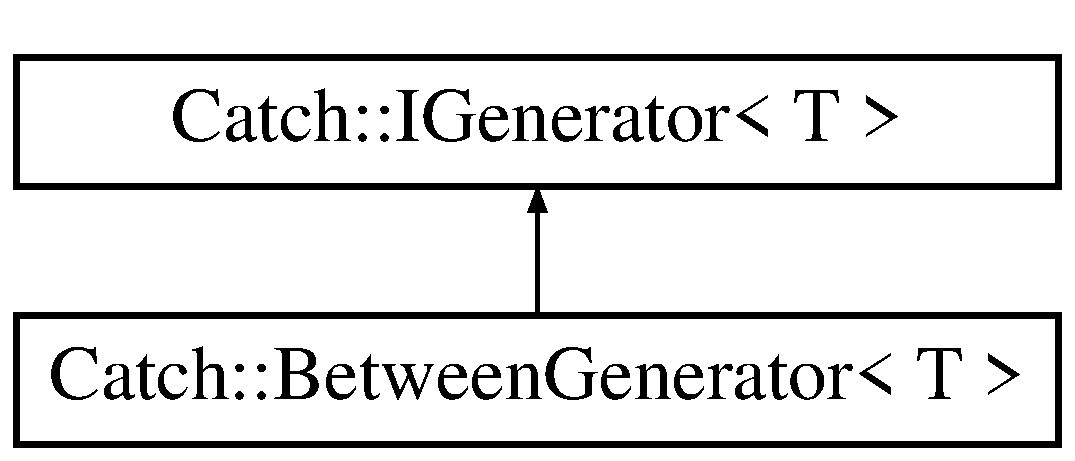
\includegraphics[height=2.000000cm]{class_catch_1_1_between_generator}
\end{center}
\end{figure}
\subsection*{Public Member Functions}
\begin{DoxyCompactItemize}
\item 
\mbox{\hyperlink{class_catch_1_1_between_generator_a835a057d691ae37caef660624099b51c}{Between\+Generator}} (T from, T to)
\item 
virtual T \mbox{\hyperlink{class_catch_1_1_between_generator_a913f74bb0c23b3bc0127abfffdabbd94}{get\+Value}} (std\+::size\+\_\+t index) const
\item 
virtual std\+::size\+\_\+t \mbox{\hyperlink{class_catch_1_1_between_generator_af65a1fe51f9b1106fc676e3dd189adb6}{size}} () const
\end{DoxyCompactItemize}


\subsection{Constructor \& Destructor Documentation}
\mbox{\Hypertarget{class_catch_1_1_between_generator_a835a057d691ae37caef660624099b51c}\label{class_catch_1_1_between_generator_a835a057d691ae37caef660624099b51c}} 
\index{Catch\+::\+Between\+Generator@{Catch\+::\+Between\+Generator}!Between\+Generator@{Between\+Generator}}
\index{Between\+Generator@{Between\+Generator}!Catch\+::\+Between\+Generator@{Catch\+::\+Between\+Generator}}
\subsubsection{\texorpdfstring{Between\+Generator()}{BetweenGenerator()}}
{\footnotesize\ttfamily template$<$typename T $>$ \\
\mbox{\hyperlink{class_catch_1_1_between_generator}{Catch\+::\+Between\+Generator}}$<$ T $>$\+::\mbox{\hyperlink{class_catch_1_1_between_generator}{Between\+Generator}} (\begin{DoxyParamCaption}\item[{T}]{from,  }\item[{T}]{to }\end{DoxyParamCaption})\hspace{0.3cm}{\ttfamily [inline]}}



\subsection{Member Function Documentation}
\mbox{\Hypertarget{class_catch_1_1_between_generator_a913f74bb0c23b3bc0127abfffdabbd94}\label{class_catch_1_1_between_generator_a913f74bb0c23b3bc0127abfffdabbd94}} 
\index{Catch\+::\+Between\+Generator@{Catch\+::\+Between\+Generator}!get\+Value@{get\+Value}}
\index{get\+Value@{get\+Value}!Catch\+::\+Between\+Generator@{Catch\+::\+Between\+Generator}}
\subsubsection{\texorpdfstring{get\+Value()}{getValue()}}
{\footnotesize\ttfamily template$<$typename T $>$ \\
virtual T \mbox{\hyperlink{class_catch_1_1_between_generator}{Catch\+::\+Between\+Generator}}$<$ T $>$\+::get\+Value (\begin{DoxyParamCaption}\item[{std\+::size\+\_\+t}]{index }\end{DoxyParamCaption}) const\hspace{0.3cm}{\ttfamily [inline]}, {\ttfamily [virtual]}}



Implements \mbox{\hyperlink{struct_catch_1_1_i_generator_ad69e937cb66dba3ed9429c42abf4fce3}{Catch\+::\+I\+Generator$<$ T $>$}}.

\mbox{\Hypertarget{class_catch_1_1_between_generator_af65a1fe51f9b1106fc676e3dd189adb6}\label{class_catch_1_1_between_generator_af65a1fe51f9b1106fc676e3dd189adb6}} 
\index{Catch\+::\+Between\+Generator@{Catch\+::\+Between\+Generator}!size@{size}}
\index{size@{size}!Catch\+::\+Between\+Generator@{Catch\+::\+Between\+Generator}}
\subsubsection{\texorpdfstring{size()}{size()}}
{\footnotesize\ttfamily template$<$typename T $>$ \\
virtual std\+::size\+\_\+t \mbox{\hyperlink{class_catch_1_1_between_generator}{Catch\+::\+Between\+Generator}}$<$ T $>$\+::size (\begin{DoxyParamCaption}{ }\end{DoxyParamCaption}) const\hspace{0.3cm}{\ttfamily [inline]}, {\ttfamily [virtual]}}



Implements \mbox{\hyperlink{struct_catch_1_1_i_generator_a2e317253b03e838b6065ce69719a198e}{Catch\+::\+I\+Generator$<$ T $>$}}.



The documentation for this class was generated from the following file\+:\begin{DoxyCompactItemize}
\item 
include/\mbox{\hyperlink{catch_8hpp}{catch.\+hpp}}\end{DoxyCompactItemize}

\hypertarget{class_catch_1_1_binary_expression}{}\section{Catch\+:\+:Binary\+Expression$<$ LhsT, Op, RhsT $>$ Class Template Reference}
\label{class_catch_1_1_binary_expression}\index{Catch\+::\+Binary\+Expression$<$ Lhs\+T, Op, Rhs\+T $>$@{Catch\+::\+Binary\+Expression$<$ Lhs\+T, Op, Rhs\+T $>$}}


{\ttfamily \#include $<$catch.\+hpp$>$}

Inheritance diagram for Catch\+:\+:Binary\+Expression$<$ LhsT, Op, RhsT $>$\+:\begin{figure}[H]
\begin{center}
\leavevmode
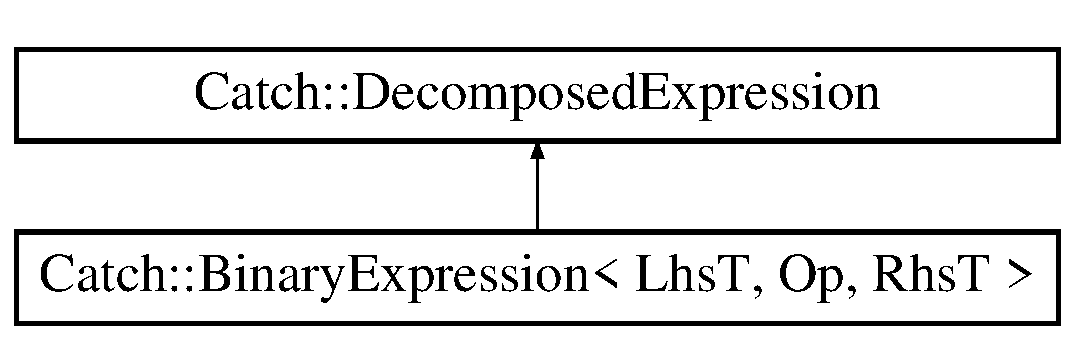
\includegraphics[height=2.000000cm]{class_catch_1_1_binary_expression}
\end{center}
\end{figure}
\subsection*{Public Member Functions}
\begin{DoxyCompactItemize}
\item 
\mbox{\hyperlink{class_catch_1_1_binary_expression_a0d81384761aba5f7a6d5f4fc7e7944f3}{Binary\+Expression}} (\mbox{\hyperlink{class_catch_1_1_result_builder}{Result\+Builder}} \&rb, LhsT lhs, RhsT rhs)
\item 
\mbox{\hyperlink{class_catch_1_1_binary_expression}{Binary\+Expression}} \& \mbox{\hyperlink{class_catch_1_1_binary_expression_a2147a858eb5866e5643d0ef321064aa1}{operator=}} (\mbox{\hyperlink{class_catch_1_1_binary_expression}{Binary\+Expression}} \&)
\item 
void \mbox{\hyperlink{class_catch_1_1_binary_expression_aa1dba7f316f70902859b8eab27692dfb}{end\+Expression}} () const
\item 
virtual bool \mbox{\hyperlink{class_catch_1_1_binary_expression_a4c617c0b6a73a9cafbbf900909c7c258}{is\+Binary\+Expression}} () const \mbox{\hyperlink{catch_8hpp_a8ecdce4d3f57835f707915ae831eb847}{C\+A\+T\+C\+H\+\_\+\+O\+V\+E\+R\+R\+I\+DE}}
\item 
virtual void \mbox{\hyperlink{class_catch_1_1_binary_expression_a6ed73ff9af9c229f9fa3d35d019f9e37}{reconstruct\+Expression}} (std\+::string \&dest) const \mbox{\hyperlink{catch_8hpp_a8ecdce4d3f57835f707915ae831eb847}{C\+A\+T\+C\+H\+\_\+\+O\+V\+E\+R\+R\+I\+DE}}
\end{DoxyCompactItemize}


\subsection{Constructor \& Destructor Documentation}
\mbox{\Hypertarget{class_catch_1_1_binary_expression_a0d81384761aba5f7a6d5f4fc7e7944f3}\label{class_catch_1_1_binary_expression_a0d81384761aba5f7a6d5f4fc7e7944f3}} 
\index{Catch\+::\+Binary\+Expression@{Catch\+::\+Binary\+Expression}!Binary\+Expression@{Binary\+Expression}}
\index{Binary\+Expression@{Binary\+Expression}!Catch\+::\+Binary\+Expression@{Catch\+::\+Binary\+Expression}}
\subsubsection{\texorpdfstring{Binary\+Expression()}{BinaryExpression()}}
{\footnotesize\ttfamily template$<$typename LhsT, Internal\+::\+Operator Op, typename RhsT$>$ \\
\mbox{\hyperlink{class_catch_1_1_binary_expression}{Catch\+::\+Binary\+Expression}}$<$ LhsT, Op, RhsT $>$\+::\mbox{\hyperlink{class_catch_1_1_binary_expression}{Binary\+Expression}} (\begin{DoxyParamCaption}\item[{\mbox{\hyperlink{class_catch_1_1_result_builder}{Result\+Builder}} \&}]{rb,  }\item[{LhsT}]{lhs,  }\item[{RhsT}]{rhs }\end{DoxyParamCaption})\hspace{0.3cm}{\ttfamily [inline]}}



\subsection{Member Function Documentation}
\mbox{\Hypertarget{class_catch_1_1_binary_expression_aa1dba7f316f70902859b8eab27692dfb}\label{class_catch_1_1_binary_expression_aa1dba7f316f70902859b8eab27692dfb}} 
\index{Catch\+::\+Binary\+Expression@{Catch\+::\+Binary\+Expression}!end\+Expression@{end\+Expression}}
\index{end\+Expression@{end\+Expression}!Catch\+::\+Binary\+Expression@{Catch\+::\+Binary\+Expression}}
\subsubsection{\texorpdfstring{end\+Expression()}{endExpression()}}
{\footnotesize\ttfamily template$<$typename LhsT, Internal\+::\+Operator Op, typename RhsT$>$ \\
void \mbox{\hyperlink{class_catch_1_1_binary_expression}{Catch\+::\+Binary\+Expression}}$<$ LhsT, Op, RhsT $>$\+::end\+Expression (\begin{DoxyParamCaption}{ }\end{DoxyParamCaption}) const\hspace{0.3cm}{\ttfamily [inline]}}

\mbox{\Hypertarget{class_catch_1_1_binary_expression_a4c617c0b6a73a9cafbbf900909c7c258}\label{class_catch_1_1_binary_expression_a4c617c0b6a73a9cafbbf900909c7c258}} 
\index{Catch\+::\+Binary\+Expression@{Catch\+::\+Binary\+Expression}!is\+Binary\+Expression@{is\+Binary\+Expression}}
\index{is\+Binary\+Expression@{is\+Binary\+Expression}!Catch\+::\+Binary\+Expression@{Catch\+::\+Binary\+Expression}}
\subsubsection{\texorpdfstring{is\+Binary\+Expression()}{isBinaryExpression()}}
{\footnotesize\ttfamily template$<$typename LhsT, Internal\+::\+Operator Op, typename RhsT$>$ \\
virtual bool \mbox{\hyperlink{class_catch_1_1_binary_expression}{Catch\+::\+Binary\+Expression}}$<$ LhsT, Op, RhsT $>$\+::is\+Binary\+Expression (\begin{DoxyParamCaption}{ }\end{DoxyParamCaption}) const\hspace{0.3cm}{\ttfamily [inline]}, {\ttfamily [virtual]}}



Reimplemented from \mbox{\hyperlink{struct_catch_1_1_decomposed_expression_a1c458ece47b71f093290dbdf9bb31fdb}{Catch\+::\+Decomposed\+Expression}}.

\mbox{\Hypertarget{class_catch_1_1_binary_expression_a2147a858eb5866e5643d0ef321064aa1}\label{class_catch_1_1_binary_expression_a2147a858eb5866e5643d0ef321064aa1}} 
\index{Catch\+::\+Binary\+Expression@{Catch\+::\+Binary\+Expression}!operator=@{operator=}}
\index{operator=@{operator=}!Catch\+::\+Binary\+Expression@{Catch\+::\+Binary\+Expression}}
\subsubsection{\texorpdfstring{operator=()}{operator=()}}
{\footnotesize\ttfamily template$<$typename LhsT, Internal\+::\+Operator Op, typename RhsT$>$ \\
\mbox{\hyperlink{class_catch_1_1_binary_expression}{Binary\+Expression}}\& \mbox{\hyperlink{class_catch_1_1_binary_expression}{Catch\+::\+Binary\+Expression}}$<$ LhsT, Op, RhsT $>$\+::operator= (\begin{DoxyParamCaption}\item[{\mbox{\hyperlink{class_catch_1_1_binary_expression}{Binary\+Expression}}$<$ LhsT, Op, RhsT $>$ \&}]{ }\end{DoxyParamCaption})}

\mbox{\Hypertarget{class_catch_1_1_binary_expression_a6ed73ff9af9c229f9fa3d35d019f9e37}\label{class_catch_1_1_binary_expression_a6ed73ff9af9c229f9fa3d35d019f9e37}} 
\index{Catch\+::\+Binary\+Expression@{Catch\+::\+Binary\+Expression}!reconstruct\+Expression@{reconstruct\+Expression}}
\index{reconstruct\+Expression@{reconstruct\+Expression}!Catch\+::\+Binary\+Expression@{Catch\+::\+Binary\+Expression}}
\subsubsection{\texorpdfstring{reconstruct\+Expression()}{reconstructExpression()}}
{\footnotesize\ttfamily template$<$typename LhsT, Internal\+::\+Operator Op, typename RhsT$>$ \\
virtual void \mbox{\hyperlink{class_catch_1_1_binary_expression}{Catch\+::\+Binary\+Expression}}$<$ LhsT, Op, RhsT $>$\+::reconstruct\+Expression (\begin{DoxyParamCaption}\item[{std\+::string \&}]{dest }\end{DoxyParamCaption}) const\hspace{0.3cm}{\ttfamily [inline]}, {\ttfamily [virtual]}}



Implements \mbox{\hyperlink{struct_catch_1_1_decomposed_expression_a9ce7f356dc96f11f80e40c82f5aa7e55}{Catch\+::\+Decomposed\+Expression}}.



The documentation for this class was generated from the following file\+:\begin{DoxyCompactItemize}
\item 
include/\mbox{\hyperlink{catch_8hpp}{catch.\+hpp}}\end{DoxyCompactItemize}

\hypertarget{struct_catch_1_1_detail_1_1_borg_type}{}\section{Catch\+:\+:Detail\+:\+:Borg\+Type Struct Reference}
\label{struct_catch_1_1_detail_1_1_borg_type}\index{Catch\+::\+Detail\+::\+Borg\+Type@{Catch\+::\+Detail\+::\+Borg\+Type}}


{\ttfamily \#include $<$catch.\+hpp$>$}

\subsection*{Public Member Functions}
\begin{DoxyCompactItemize}
\item 
{\footnotesize template$<$typename T $>$ }\\\mbox{\hyperlink{struct_catch_1_1_detail_1_1_borg_type_a780a9946ed0d654f0bfc043c8fc505d8}{Borg\+Type}} (T const \&)
\end{DoxyCompactItemize}


\subsection{Constructor \& Destructor Documentation}
\mbox{\Hypertarget{struct_catch_1_1_detail_1_1_borg_type_a780a9946ed0d654f0bfc043c8fc505d8}\label{struct_catch_1_1_detail_1_1_borg_type_a780a9946ed0d654f0bfc043c8fc505d8}} 
\index{Catch\+::\+Detail\+::\+Borg\+Type@{Catch\+::\+Detail\+::\+Borg\+Type}!Borg\+Type@{Borg\+Type}}
\index{Borg\+Type@{Borg\+Type}!Catch\+::\+Detail\+::\+Borg\+Type@{Catch\+::\+Detail\+::\+Borg\+Type}}
\subsubsection{\texorpdfstring{Borg\+Type()}{BorgType()}}
{\footnotesize\ttfamily template$<$typename T $>$ \\
Catch\+::\+Detail\+::\+Borg\+Type\+::\+Borg\+Type (\begin{DoxyParamCaption}\item[{T const \&}]{ }\end{DoxyParamCaption})}



The documentation for this struct was generated from the following file\+:\begin{DoxyCompactItemize}
\item 
include/\mbox{\hyperlink{catch_8hpp}{catch.\+hpp}}\end{DoxyCompactItemize}

\hypertarget{struct_catch_1_1_matchers_1_1_std_string_1_1_cased_string}{}\section{Catch\+:\+:Matchers\+:\+:Std\+String\+:\+:Cased\+String Struct Reference}
\label{struct_catch_1_1_matchers_1_1_std_string_1_1_cased_string}\index{Catch\+::\+Matchers\+::\+Std\+String\+::\+Cased\+String@{Catch\+::\+Matchers\+::\+Std\+String\+::\+Cased\+String}}


{\ttfamily \#include $<$catch.\+hpp$>$}

\subsection*{Public Member Functions}
\begin{DoxyCompactItemize}
\item 
\mbox{\hyperlink{struct_catch_1_1_matchers_1_1_std_string_1_1_cased_string_aa88bbc5acd2bff22351d8d4b1816b561}{Cased\+String}} (std\+::string const \&str, \mbox{\hyperlink{struct_catch_1_1_case_sensitive_aad49d3aee2d97066642fffa919685c6a}{Case\+Sensitive\+::\+Choice}} case\+Sensitivity)
\item 
std\+::string \mbox{\hyperlink{struct_catch_1_1_matchers_1_1_std_string_1_1_cased_string_a77639b1165c01f424ee0e96f53335010}{adjust\+String}} (std\+::string const \&str) const
\item 
std\+::string \mbox{\hyperlink{struct_catch_1_1_matchers_1_1_std_string_1_1_cased_string_a9759155344d696b2476d764a1d95fcc9}{case\+Sensitivity\+Suffix}} () const
\end{DoxyCompactItemize}
\subsection*{Public Attributes}
\begin{DoxyCompactItemize}
\item 
\mbox{\hyperlink{struct_catch_1_1_case_sensitive_aad49d3aee2d97066642fffa919685c6a}{Case\+Sensitive\+::\+Choice}} \mbox{\hyperlink{struct_catch_1_1_matchers_1_1_std_string_1_1_cased_string_ae1c2864c986941536a6e94cca0528f92}{m\+\_\+case\+Sensitivity}}
\item 
std\+::string \mbox{\hyperlink{struct_catch_1_1_matchers_1_1_std_string_1_1_cased_string_ad05dbc99aba3c3c386d6b856b213f911}{m\+\_\+str}}
\end{DoxyCompactItemize}


\subsection{Constructor \& Destructor Documentation}
\mbox{\Hypertarget{struct_catch_1_1_matchers_1_1_std_string_1_1_cased_string_aa88bbc5acd2bff22351d8d4b1816b561}\label{struct_catch_1_1_matchers_1_1_std_string_1_1_cased_string_aa88bbc5acd2bff22351d8d4b1816b561}} 
\index{Catch\+::\+Matchers\+::\+Std\+String\+::\+Cased\+String@{Catch\+::\+Matchers\+::\+Std\+String\+::\+Cased\+String}!Cased\+String@{Cased\+String}}
\index{Cased\+String@{Cased\+String}!Catch\+::\+Matchers\+::\+Std\+String\+::\+Cased\+String@{Catch\+::\+Matchers\+::\+Std\+String\+::\+Cased\+String}}
\subsubsection{\texorpdfstring{Cased\+String()}{CasedString()}}
{\footnotesize\ttfamily Catch\+::\+Matchers\+::\+Std\+String\+::\+Cased\+String\+::\+Cased\+String (\begin{DoxyParamCaption}\item[{std\+::string const \&}]{str,  }\item[{\mbox{\hyperlink{struct_catch_1_1_case_sensitive_aad49d3aee2d97066642fffa919685c6a}{Case\+Sensitive\+::\+Choice}}}]{case\+Sensitivity }\end{DoxyParamCaption})}



\subsection{Member Function Documentation}
\mbox{\Hypertarget{struct_catch_1_1_matchers_1_1_std_string_1_1_cased_string_a77639b1165c01f424ee0e96f53335010}\label{struct_catch_1_1_matchers_1_1_std_string_1_1_cased_string_a77639b1165c01f424ee0e96f53335010}} 
\index{Catch\+::\+Matchers\+::\+Std\+String\+::\+Cased\+String@{Catch\+::\+Matchers\+::\+Std\+String\+::\+Cased\+String}!adjust\+String@{adjust\+String}}
\index{adjust\+String@{adjust\+String}!Catch\+::\+Matchers\+::\+Std\+String\+::\+Cased\+String@{Catch\+::\+Matchers\+::\+Std\+String\+::\+Cased\+String}}
\subsubsection{\texorpdfstring{adjust\+String()}{adjustString()}}
{\footnotesize\ttfamily std\+::string Catch\+::\+Matchers\+::\+Std\+String\+::\+Cased\+String\+::adjust\+String (\begin{DoxyParamCaption}\item[{std\+::string const \&}]{str }\end{DoxyParamCaption}) const}

\mbox{\Hypertarget{struct_catch_1_1_matchers_1_1_std_string_1_1_cased_string_a9759155344d696b2476d764a1d95fcc9}\label{struct_catch_1_1_matchers_1_1_std_string_1_1_cased_string_a9759155344d696b2476d764a1d95fcc9}} 
\index{Catch\+::\+Matchers\+::\+Std\+String\+::\+Cased\+String@{Catch\+::\+Matchers\+::\+Std\+String\+::\+Cased\+String}!case\+Sensitivity\+Suffix@{case\+Sensitivity\+Suffix}}
\index{case\+Sensitivity\+Suffix@{case\+Sensitivity\+Suffix}!Catch\+::\+Matchers\+::\+Std\+String\+::\+Cased\+String@{Catch\+::\+Matchers\+::\+Std\+String\+::\+Cased\+String}}
\subsubsection{\texorpdfstring{case\+Sensitivity\+Suffix()}{caseSensitivitySuffix()}}
{\footnotesize\ttfamily std\+::string Catch\+::\+Matchers\+::\+Std\+String\+::\+Cased\+String\+::case\+Sensitivity\+Suffix (\begin{DoxyParamCaption}{ }\end{DoxyParamCaption}) const}



\subsection{Member Data Documentation}
\mbox{\Hypertarget{struct_catch_1_1_matchers_1_1_std_string_1_1_cased_string_ae1c2864c986941536a6e94cca0528f92}\label{struct_catch_1_1_matchers_1_1_std_string_1_1_cased_string_ae1c2864c986941536a6e94cca0528f92}} 
\index{Catch\+::\+Matchers\+::\+Std\+String\+::\+Cased\+String@{Catch\+::\+Matchers\+::\+Std\+String\+::\+Cased\+String}!m\+\_\+case\+Sensitivity@{m\+\_\+case\+Sensitivity}}
\index{m\+\_\+case\+Sensitivity@{m\+\_\+case\+Sensitivity}!Catch\+::\+Matchers\+::\+Std\+String\+::\+Cased\+String@{Catch\+::\+Matchers\+::\+Std\+String\+::\+Cased\+String}}
\subsubsection{\texorpdfstring{m\+\_\+case\+Sensitivity}{m\_caseSensitivity}}
{\footnotesize\ttfamily \mbox{\hyperlink{struct_catch_1_1_case_sensitive_aad49d3aee2d97066642fffa919685c6a}{Case\+Sensitive\+::\+Choice}} Catch\+::\+Matchers\+::\+Std\+String\+::\+Cased\+String\+::m\+\_\+case\+Sensitivity}

\mbox{\Hypertarget{struct_catch_1_1_matchers_1_1_std_string_1_1_cased_string_ad05dbc99aba3c3c386d6b856b213f911}\label{struct_catch_1_1_matchers_1_1_std_string_1_1_cased_string_ad05dbc99aba3c3c386d6b856b213f911}} 
\index{Catch\+::\+Matchers\+::\+Std\+String\+::\+Cased\+String@{Catch\+::\+Matchers\+::\+Std\+String\+::\+Cased\+String}!m\+\_\+str@{m\+\_\+str}}
\index{m\+\_\+str@{m\+\_\+str}!Catch\+::\+Matchers\+::\+Std\+String\+::\+Cased\+String@{Catch\+::\+Matchers\+::\+Std\+String\+::\+Cased\+String}}
\subsubsection{\texorpdfstring{m\+\_\+str}{m\_str}}
{\footnotesize\ttfamily std\+::string Catch\+::\+Matchers\+::\+Std\+String\+::\+Cased\+String\+::m\+\_\+str}



The documentation for this struct was generated from the following file\+:\begin{DoxyCompactItemize}
\item 
include/\mbox{\hyperlink{catch_8hpp}{catch.\+hpp}}\end{DoxyCompactItemize}

\hypertarget{struct_catch_1_1_case_sensitive}{}\section{Catch\+:\+:Case\+Sensitive Struct Reference}
\label{struct_catch_1_1_case_sensitive}\index{Catch\+::\+Case\+Sensitive@{Catch\+::\+Case\+Sensitive}}


{\ttfamily \#include $<$catch.\+hpp$>$}

\subsection*{Public Types}
\begin{DoxyCompactItemize}
\item 
enum \mbox{\hyperlink{struct_catch_1_1_case_sensitive_aad49d3aee2d97066642fffa919685c6a}{Choice}} \{ \mbox{\hyperlink{struct_catch_1_1_case_sensitive_aad49d3aee2d97066642fffa919685c6aa7c5550b69ec3c502e6f609b67f9613c6}{Yes}}, 
\mbox{\hyperlink{struct_catch_1_1_case_sensitive_aad49d3aee2d97066642fffa919685c6aa4ffff8d29b481f0116abc37228cd53f6}{No}}
 \}
\end{DoxyCompactItemize}


\subsection{Member Enumeration Documentation}
\mbox{\Hypertarget{struct_catch_1_1_case_sensitive_aad49d3aee2d97066642fffa919685c6a}\label{struct_catch_1_1_case_sensitive_aad49d3aee2d97066642fffa919685c6a}} 
\index{Catch\+::\+Case\+Sensitive@{Catch\+::\+Case\+Sensitive}!Choice@{Choice}}
\index{Choice@{Choice}!Catch\+::\+Case\+Sensitive@{Catch\+::\+Case\+Sensitive}}
\subsubsection{\texorpdfstring{Choice}{Choice}}
{\footnotesize\ttfamily enum \mbox{\hyperlink{struct_catch_1_1_case_sensitive_aad49d3aee2d97066642fffa919685c6a}{Catch\+::\+Case\+Sensitive\+::\+Choice}}}

\begin{DoxyEnumFields}{Enumerator}
\raisebox{\heightof{T}}[0pt][0pt]{\index{Yes@{Yes}!Catch\+::\+Case\+Sensitive@{Catch\+::\+Case\+Sensitive}}\index{Catch\+::\+Case\+Sensitive@{Catch\+::\+Case\+Sensitive}!Yes@{Yes}}}\mbox{\Hypertarget{struct_catch_1_1_case_sensitive_aad49d3aee2d97066642fffa919685c6aa7c5550b69ec3c502e6f609b67f9613c6}\label{struct_catch_1_1_case_sensitive_aad49d3aee2d97066642fffa919685c6aa7c5550b69ec3c502e6f609b67f9613c6}} 
Yes&\\
\hline

\raisebox{\heightof{T}}[0pt][0pt]{\index{No@{No}!Catch\+::\+Case\+Sensitive@{Catch\+::\+Case\+Sensitive}}\index{Catch\+::\+Case\+Sensitive@{Catch\+::\+Case\+Sensitive}!No@{No}}}\mbox{\Hypertarget{struct_catch_1_1_case_sensitive_aad49d3aee2d97066642fffa919685c6aa4ffff8d29b481f0116abc37228cd53f6}\label{struct_catch_1_1_case_sensitive_aad49d3aee2d97066642fffa919685c6aa4ffff8d29b481f0116abc37228cd53f6}} 
No&\\
\hline

\end{DoxyEnumFields}


The documentation for this struct was generated from the following file\+:\begin{DoxyCompactItemize}
\item 
include/\mbox{\hyperlink{catch_8hpp}{catch.\+hpp}}\end{DoxyCompactItemize}

\hypertarget{class_catch_1_1_composite_generator}{}\section{Catch\+:\+:Composite\+Generator$<$ T $>$ Class Template Reference}
\label{class_catch_1_1_composite_generator}\index{Catch\+::\+Composite\+Generator$<$ T $>$@{Catch\+::\+Composite\+Generator$<$ T $>$}}


{\ttfamily \#include $<$catch.\+hpp$>$}

\subsection*{Public Member Functions}
\begin{DoxyCompactItemize}
\item 
\mbox{\hyperlink{class_catch_1_1_composite_generator_a923398b140371d1783858766864a1af5}{Composite\+Generator}} ()
\item 
\mbox{\hyperlink{class_catch_1_1_composite_generator_a21a7070a00e4a6fe021294c356692692}{Composite\+Generator}} (\mbox{\hyperlink{class_catch_1_1_composite_generator}{Composite\+Generator}} \&other)
\item 
\mbox{\hyperlink{class_catch_1_1_composite_generator}{Composite\+Generator}} \& \mbox{\hyperlink{class_catch_1_1_composite_generator_ac3c57cf4ca5472f440bf71e2936bcd4a}{set\+File\+Info}} (const char $\ast$file\+Info)
\item 
\mbox{\hyperlink{class_catch_1_1_composite_generator_a5766205abd7004c508c20ddbb5e5555e}{$\sim$\+Composite\+Generator}} ()
\item 
\mbox{\hyperlink{class_catch_1_1_composite_generator_a83d6c941e2e735b9528e6e832f7b76e7}{operator T}} () const
\item 
void \mbox{\hyperlink{class_catch_1_1_composite_generator_af3774d42ad2d3453d089ca599efe0517}{add}} (const \mbox{\hyperlink{struct_catch_1_1_i_generator}{I\+Generator}}$<$ T $>$ $\ast$generator)
\item 
\mbox{\hyperlink{class_catch_1_1_composite_generator}{Composite\+Generator}} \& \mbox{\hyperlink{class_catch_1_1_composite_generator_a2e03f42df85cdd238aabd77a80b075d5}{then}} (\mbox{\hyperlink{class_catch_1_1_composite_generator}{Composite\+Generator}} \&other)
\item 
\mbox{\hyperlink{class_catch_1_1_composite_generator}{Composite\+Generator}} \& \mbox{\hyperlink{class_catch_1_1_composite_generator_aefdc11bcfccdf07d2db5f0da3ed8758c}{then}} (T value)
\end{DoxyCompactItemize}


\subsection{Constructor \& Destructor Documentation}
\mbox{\Hypertarget{class_catch_1_1_composite_generator_a923398b140371d1783858766864a1af5}\label{class_catch_1_1_composite_generator_a923398b140371d1783858766864a1af5}} 
\index{Catch\+::\+Composite\+Generator@{Catch\+::\+Composite\+Generator}!Composite\+Generator@{Composite\+Generator}}
\index{Composite\+Generator@{Composite\+Generator}!Catch\+::\+Composite\+Generator@{Catch\+::\+Composite\+Generator}}
\subsubsection{\texorpdfstring{Composite\+Generator()}{CompositeGenerator()}\hspace{0.1cm}{\footnotesize\ttfamily [1/2]}}
{\footnotesize\ttfamily template$<$typename T$>$ \\
\mbox{\hyperlink{class_catch_1_1_composite_generator}{Catch\+::\+Composite\+Generator}}$<$ T $>$\+::\mbox{\hyperlink{class_catch_1_1_composite_generator}{Composite\+Generator}} (\begin{DoxyParamCaption}{ }\end{DoxyParamCaption})\hspace{0.3cm}{\ttfamily [inline]}}

\mbox{\Hypertarget{class_catch_1_1_composite_generator_a21a7070a00e4a6fe021294c356692692}\label{class_catch_1_1_composite_generator_a21a7070a00e4a6fe021294c356692692}} 
\index{Catch\+::\+Composite\+Generator@{Catch\+::\+Composite\+Generator}!Composite\+Generator@{Composite\+Generator}}
\index{Composite\+Generator@{Composite\+Generator}!Catch\+::\+Composite\+Generator@{Catch\+::\+Composite\+Generator}}
\subsubsection{\texorpdfstring{Composite\+Generator()}{CompositeGenerator()}\hspace{0.1cm}{\footnotesize\ttfamily [2/2]}}
{\footnotesize\ttfamily template$<$typename T$>$ \\
\mbox{\hyperlink{class_catch_1_1_composite_generator}{Catch\+::\+Composite\+Generator}}$<$ T $>$\+::\mbox{\hyperlink{class_catch_1_1_composite_generator}{Composite\+Generator}} (\begin{DoxyParamCaption}\item[{\mbox{\hyperlink{class_catch_1_1_composite_generator}{Composite\+Generator}}$<$ T $>$ \&}]{other }\end{DoxyParamCaption})\hspace{0.3cm}{\ttfamily [inline]}}

\mbox{\Hypertarget{class_catch_1_1_composite_generator_a5766205abd7004c508c20ddbb5e5555e}\label{class_catch_1_1_composite_generator_a5766205abd7004c508c20ddbb5e5555e}} 
\index{Catch\+::\+Composite\+Generator@{Catch\+::\+Composite\+Generator}!````~Composite\+Generator@{$\sim$\+Composite\+Generator}}
\index{````~Composite\+Generator@{$\sim$\+Composite\+Generator}!Catch\+::\+Composite\+Generator@{Catch\+::\+Composite\+Generator}}
\subsubsection{\texorpdfstring{$\sim$\+Composite\+Generator()}{~CompositeGenerator()}}
{\footnotesize\ttfamily template$<$typename T$>$ \\
\mbox{\hyperlink{class_catch_1_1_composite_generator}{Catch\+::\+Composite\+Generator}}$<$ T $>$\+::$\sim$\mbox{\hyperlink{class_catch_1_1_composite_generator}{Composite\+Generator}} (\begin{DoxyParamCaption}{ }\end{DoxyParamCaption})\hspace{0.3cm}{\ttfamily [inline]}}



\subsection{Member Function Documentation}
\mbox{\Hypertarget{class_catch_1_1_composite_generator_af3774d42ad2d3453d089ca599efe0517}\label{class_catch_1_1_composite_generator_af3774d42ad2d3453d089ca599efe0517}} 
\index{Catch\+::\+Composite\+Generator@{Catch\+::\+Composite\+Generator}!add@{add}}
\index{add@{add}!Catch\+::\+Composite\+Generator@{Catch\+::\+Composite\+Generator}}
\subsubsection{\texorpdfstring{add()}{add()}}
{\footnotesize\ttfamily template$<$typename T$>$ \\
void \mbox{\hyperlink{class_catch_1_1_composite_generator}{Catch\+::\+Composite\+Generator}}$<$ T $>$\+::add (\begin{DoxyParamCaption}\item[{const \mbox{\hyperlink{struct_catch_1_1_i_generator}{I\+Generator}}$<$ T $>$ $\ast$}]{generator }\end{DoxyParamCaption})\hspace{0.3cm}{\ttfamily [inline]}}

\mbox{\Hypertarget{class_catch_1_1_composite_generator_a83d6c941e2e735b9528e6e832f7b76e7}\label{class_catch_1_1_composite_generator_a83d6c941e2e735b9528e6e832f7b76e7}} 
\index{Catch\+::\+Composite\+Generator@{Catch\+::\+Composite\+Generator}!operator T@{operator T}}
\index{operator T@{operator T}!Catch\+::\+Composite\+Generator@{Catch\+::\+Composite\+Generator}}
\subsubsection{\texorpdfstring{operator T()}{operator T()}}
{\footnotesize\ttfamily template$<$typename T$>$ \\
\mbox{\hyperlink{class_catch_1_1_composite_generator}{Catch\+::\+Composite\+Generator}}$<$ T $>$\+::operator T (\begin{DoxyParamCaption}{ }\end{DoxyParamCaption}) const\hspace{0.3cm}{\ttfamily [inline]}}

\mbox{\Hypertarget{class_catch_1_1_composite_generator_ac3c57cf4ca5472f440bf71e2936bcd4a}\label{class_catch_1_1_composite_generator_ac3c57cf4ca5472f440bf71e2936bcd4a}} 
\index{Catch\+::\+Composite\+Generator@{Catch\+::\+Composite\+Generator}!set\+File\+Info@{set\+File\+Info}}
\index{set\+File\+Info@{set\+File\+Info}!Catch\+::\+Composite\+Generator@{Catch\+::\+Composite\+Generator}}
\subsubsection{\texorpdfstring{set\+File\+Info()}{setFileInfo()}}
{\footnotesize\ttfamily template$<$typename T$>$ \\
\mbox{\hyperlink{class_catch_1_1_composite_generator}{Composite\+Generator}}\& \mbox{\hyperlink{class_catch_1_1_composite_generator}{Catch\+::\+Composite\+Generator}}$<$ T $>$\+::set\+File\+Info (\begin{DoxyParamCaption}\item[{const char $\ast$}]{file\+Info }\end{DoxyParamCaption})\hspace{0.3cm}{\ttfamily [inline]}}

\mbox{\Hypertarget{class_catch_1_1_composite_generator_a2e03f42df85cdd238aabd77a80b075d5}\label{class_catch_1_1_composite_generator_a2e03f42df85cdd238aabd77a80b075d5}} 
\index{Catch\+::\+Composite\+Generator@{Catch\+::\+Composite\+Generator}!then@{then}}
\index{then@{then}!Catch\+::\+Composite\+Generator@{Catch\+::\+Composite\+Generator}}
\subsubsection{\texorpdfstring{then()}{then()}\hspace{0.1cm}{\footnotesize\ttfamily [1/2]}}
{\footnotesize\ttfamily template$<$typename T$>$ \\
\mbox{\hyperlink{class_catch_1_1_composite_generator}{Composite\+Generator}}\& \mbox{\hyperlink{class_catch_1_1_composite_generator}{Catch\+::\+Composite\+Generator}}$<$ T $>$\+::then (\begin{DoxyParamCaption}\item[{\mbox{\hyperlink{class_catch_1_1_composite_generator}{Composite\+Generator}}$<$ T $>$ \&}]{other }\end{DoxyParamCaption})\hspace{0.3cm}{\ttfamily [inline]}}

\mbox{\Hypertarget{class_catch_1_1_composite_generator_aefdc11bcfccdf07d2db5f0da3ed8758c}\label{class_catch_1_1_composite_generator_aefdc11bcfccdf07d2db5f0da3ed8758c}} 
\index{Catch\+::\+Composite\+Generator@{Catch\+::\+Composite\+Generator}!then@{then}}
\index{then@{then}!Catch\+::\+Composite\+Generator@{Catch\+::\+Composite\+Generator}}
\subsubsection{\texorpdfstring{then()}{then()}\hspace{0.1cm}{\footnotesize\ttfamily [2/2]}}
{\footnotesize\ttfamily template$<$typename T$>$ \\
\mbox{\hyperlink{class_catch_1_1_composite_generator}{Composite\+Generator}}\& \mbox{\hyperlink{class_catch_1_1_composite_generator}{Catch\+::\+Composite\+Generator}}$<$ T $>$\+::then (\begin{DoxyParamCaption}\item[{T}]{value }\end{DoxyParamCaption})\hspace{0.3cm}{\ttfamily [inline]}}



The documentation for this class was generated from the following file\+:\begin{DoxyCompactItemize}
\item 
include/\mbox{\hyperlink{catch_8hpp}{catch.\+hpp}}\end{DoxyCompactItemize}

\hypertarget{struct_catch_1_1_matchers_1_1_vector_1_1_contains_element_matcher}{}\section{Catch\+:\+:Matchers\+:\+:Vector\+:\+:Contains\+Element\+Matcher$<$ T $>$ Struct Template Reference}
\label{struct_catch_1_1_matchers_1_1_vector_1_1_contains_element_matcher}\index{Catch\+::\+Matchers\+::\+Vector\+::\+Contains\+Element\+Matcher$<$ T $>$@{Catch\+::\+Matchers\+::\+Vector\+::\+Contains\+Element\+Matcher$<$ T $>$}}


{\ttfamily \#include $<$catch.\+hpp$>$}

Inheritance diagram for Catch\+:\+:Matchers\+:\+:Vector\+:\+:Contains\+Element\+Matcher$<$ T $>$\+:\begin{figure}[H]
\begin{center}
\leavevmode
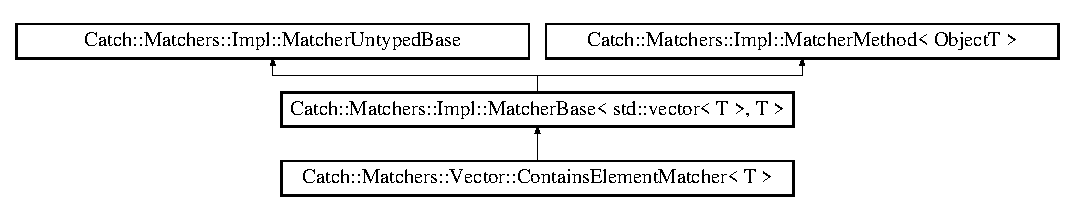
\includegraphics[height=2.400000cm]{struct_catch_1_1_matchers_1_1_vector_1_1_contains_element_matcher}
\end{center}
\end{figure}
\subsection*{Public Member Functions}
\begin{DoxyCompactItemize}
\item 
\mbox{\hyperlink{struct_catch_1_1_matchers_1_1_vector_1_1_contains_element_matcher_a6a05740b5d3f89fac8de84ac0cff7b93}{Contains\+Element\+Matcher}} (T const \&comparator)
\item 
bool \mbox{\hyperlink{struct_catch_1_1_matchers_1_1_vector_1_1_contains_element_matcher_a95fd99879bcfbe129898bef922c92c17}{match}} (std\+::vector$<$ T $>$ const \&v) const \mbox{\hyperlink{catch_8hpp_a8ecdce4d3f57835f707915ae831eb847}{C\+A\+T\+C\+H\+\_\+\+O\+V\+E\+R\+R\+I\+DE}}
\item 
virtual std\+::string \mbox{\hyperlink{struct_catch_1_1_matchers_1_1_vector_1_1_contains_element_matcher_a5a869772714dd045816707b74b217664}{describe}} () const \mbox{\hyperlink{catch_8hpp_a8ecdce4d3f57835f707915ae831eb847}{C\+A\+T\+C\+H\+\_\+\+O\+V\+E\+R\+R\+I\+DE}}
\end{DoxyCompactItemize}
\subsection*{Public Attributes}
\begin{DoxyCompactItemize}
\item 
T const  \& \mbox{\hyperlink{struct_catch_1_1_matchers_1_1_vector_1_1_contains_element_matcher_ab7eada6c4bbce1d21b44773262f9cb23}{m\+\_\+comparator}}
\end{DoxyCompactItemize}
\subsection*{Additional Inherited Members}


\subsection{Constructor \& Destructor Documentation}
\mbox{\Hypertarget{struct_catch_1_1_matchers_1_1_vector_1_1_contains_element_matcher_a6a05740b5d3f89fac8de84ac0cff7b93}\label{struct_catch_1_1_matchers_1_1_vector_1_1_contains_element_matcher_a6a05740b5d3f89fac8de84ac0cff7b93}} 
\index{Catch\+::\+Matchers\+::\+Vector\+::\+Contains\+Element\+Matcher@{Catch\+::\+Matchers\+::\+Vector\+::\+Contains\+Element\+Matcher}!Contains\+Element\+Matcher@{Contains\+Element\+Matcher}}
\index{Contains\+Element\+Matcher@{Contains\+Element\+Matcher}!Catch\+::\+Matchers\+::\+Vector\+::\+Contains\+Element\+Matcher@{Catch\+::\+Matchers\+::\+Vector\+::\+Contains\+Element\+Matcher}}
\subsubsection{\texorpdfstring{Contains\+Element\+Matcher()}{ContainsElementMatcher()}}
{\footnotesize\ttfamily template$<$typename T $>$ \\
\mbox{\hyperlink{struct_catch_1_1_matchers_1_1_vector_1_1_contains_element_matcher}{Catch\+::\+Matchers\+::\+Vector\+::\+Contains\+Element\+Matcher}}$<$ T $>$\+::\mbox{\hyperlink{struct_catch_1_1_matchers_1_1_vector_1_1_contains_element_matcher}{Contains\+Element\+Matcher}} (\begin{DoxyParamCaption}\item[{T const \&}]{comparator }\end{DoxyParamCaption})\hspace{0.3cm}{\ttfamily [inline]}}



\subsection{Member Function Documentation}
\mbox{\Hypertarget{struct_catch_1_1_matchers_1_1_vector_1_1_contains_element_matcher_a5a869772714dd045816707b74b217664}\label{struct_catch_1_1_matchers_1_1_vector_1_1_contains_element_matcher_a5a869772714dd045816707b74b217664}} 
\index{Catch\+::\+Matchers\+::\+Vector\+::\+Contains\+Element\+Matcher@{Catch\+::\+Matchers\+::\+Vector\+::\+Contains\+Element\+Matcher}!describe@{describe}}
\index{describe@{describe}!Catch\+::\+Matchers\+::\+Vector\+::\+Contains\+Element\+Matcher@{Catch\+::\+Matchers\+::\+Vector\+::\+Contains\+Element\+Matcher}}
\subsubsection{\texorpdfstring{describe()}{describe()}}
{\footnotesize\ttfamily template$<$typename T $>$ \\
virtual std\+::string \mbox{\hyperlink{struct_catch_1_1_matchers_1_1_vector_1_1_contains_element_matcher}{Catch\+::\+Matchers\+::\+Vector\+::\+Contains\+Element\+Matcher}}$<$ T $>$\+::describe (\begin{DoxyParamCaption}{ }\end{DoxyParamCaption}) const\hspace{0.3cm}{\ttfamily [inline]}, {\ttfamily [virtual]}}



Implements \mbox{\hyperlink{class_catch_1_1_matchers_1_1_impl_1_1_matcher_untyped_base_a91d3a907dbfcbb596077df24f6e11fe2}{Catch\+::\+Matchers\+::\+Impl\+::\+Matcher\+Untyped\+Base}}.

\mbox{\Hypertarget{struct_catch_1_1_matchers_1_1_vector_1_1_contains_element_matcher_a95fd99879bcfbe129898bef922c92c17}\label{struct_catch_1_1_matchers_1_1_vector_1_1_contains_element_matcher_a95fd99879bcfbe129898bef922c92c17}} 
\index{Catch\+::\+Matchers\+::\+Vector\+::\+Contains\+Element\+Matcher@{Catch\+::\+Matchers\+::\+Vector\+::\+Contains\+Element\+Matcher}!match@{match}}
\index{match@{match}!Catch\+::\+Matchers\+::\+Vector\+::\+Contains\+Element\+Matcher@{Catch\+::\+Matchers\+::\+Vector\+::\+Contains\+Element\+Matcher}}
\subsubsection{\texorpdfstring{match()}{match()}}
{\footnotesize\ttfamily template$<$typename T $>$ \\
bool \mbox{\hyperlink{struct_catch_1_1_matchers_1_1_vector_1_1_contains_element_matcher}{Catch\+::\+Matchers\+::\+Vector\+::\+Contains\+Element\+Matcher}}$<$ T $>$\+::match (\begin{DoxyParamCaption}\item[{std\+::vector$<$ T $>$ const \&}]{v }\end{DoxyParamCaption}) const\hspace{0.3cm}{\ttfamily [inline]}}



\subsection{Member Data Documentation}
\mbox{\Hypertarget{struct_catch_1_1_matchers_1_1_vector_1_1_contains_element_matcher_ab7eada6c4bbce1d21b44773262f9cb23}\label{struct_catch_1_1_matchers_1_1_vector_1_1_contains_element_matcher_ab7eada6c4bbce1d21b44773262f9cb23}} 
\index{Catch\+::\+Matchers\+::\+Vector\+::\+Contains\+Element\+Matcher@{Catch\+::\+Matchers\+::\+Vector\+::\+Contains\+Element\+Matcher}!m\+\_\+comparator@{m\+\_\+comparator}}
\index{m\+\_\+comparator@{m\+\_\+comparator}!Catch\+::\+Matchers\+::\+Vector\+::\+Contains\+Element\+Matcher@{Catch\+::\+Matchers\+::\+Vector\+::\+Contains\+Element\+Matcher}}
\subsubsection{\texorpdfstring{m\+\_\+comparator}{m\_comparator}}
{\footnotesize\ttfamily template$<$typename T $>$ \\
T const\& \mbox{\hyperlink{struct_catch_1_1_matchers_1_1_vector_1_1_contains_element_matcher}{Catch\+::\+Matchers\+::\+Vector\+::\+Contains\+Element\+Matcher}}$<$ T $>$\+::m\+\_\+comparator}



The documentation for this struct was generated from the following file\+:\begin{DoxyCompactItemize}
\item 
include/\mbox{\hyperlink{catch_8hpp}{catch.\+hpp}}\end{DoxyCompactItemize}

\hypertarget{struct_catch_1_1_matchers_1_1_std_string_1_1_contains_matcher}{}\section{Catch\+:\+:Matchers\+:\+:Std\+String\+:\+:Contains\+Matcher Struct Reference}
\label{struct_catch_1_1_matchers_1_1_std_string_1_1_contains_matcher}\index{Catch\+::\+Matchers\+::\+Std\+String\+::\+Contains\+Matcher@{Catch\+::\+Matchers\+::\+Std\+String\+::\+Contains\+Matcher}}


{\ttfamily \#include $<$catch.\+hpp$>$}

Inheritance diagram for Catch\+:\+:Matchers\+:\+:Std\+String\+:\+:Contains\+Matcher\+:\begin{figure}[H]
\begin{center}
\leavevmode
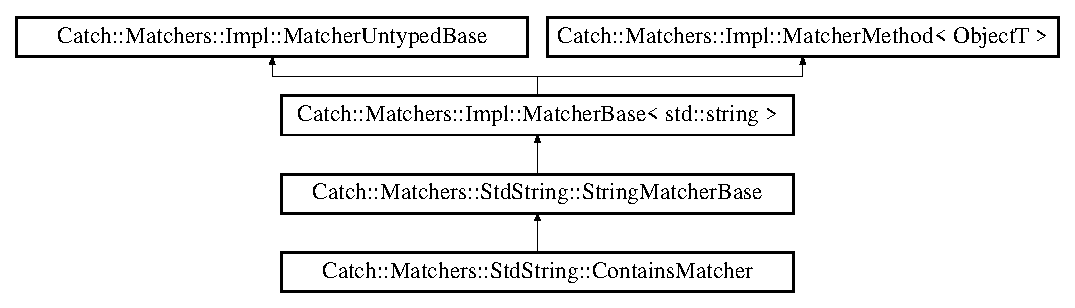
\includegraphics[height=3.696370cm]{struct_catch_1_1_matchers_1_1_std_string_1_1_contains_matcher}
\end{center}
\end{figure}
\subsection*{Public Member Functions}
\begin{DoxyCompactItemize}
\item 
\mbox{\hyperlink{struct_catch_1_1_matchers_1_1_std_string_1_1_contains_matcher_acc892883c8409e34b28c9b39d4ef1fe3}{Contains\+Matcher}} (\mbox{\hyperlink{struct_catch_1_1_matchers_1_1_std_string_1_1_cased_string}{Cased\+String}} const \&comparator)
\item 
virtual bool \mbox{\hyperlink{struct_catch_1_1_matchers_1_1_std_string_1_1_contains_matcher_ae4d567347fa563e365f1044f29ab1042}{match}} (std\+::string const \&source) const \mbox{\hyperlink{catch_8hpp_a8ecdce4d3f57835f707915ae831eb847}{C\+A\+T\+C\+H\+\_\+\+O\+V\+E\+R\+R\+I\+DE}}
\end{DoxyCompactItemize}
\subsection*{Additional Inherited Members}


\subsection{Constructor \& Destructor Documentation}
\mbox{\Hypertarget{struct_catch_1_1_matchers_1_1_std_string_1_1_contains_matcher_acc892883c8409e34b28c9b39d4ef1fe3}\label{struct_catch_1_1_matchers_1_1_std_string_1_1_contains_matcher_acc892883c8409e34b28c9b39d4ef1fe3}} 
\index{Catch\+::\+Matchers\+::\+Std\+String\+::\+Contains\+Matcher@{Catch\+::\+Matchers\+::\+Std\+String\+::\+Contains\+Matcher}!Contains\+Matcher@{Contains\+Matcher}}
\index{Contains\+Matcher@{Contains\+Matcher}!Catch\+::\+Matchers\+::\+Std\+String\+::\+Contains\+Matcher@{Catch\+::\+Matchers\+::\+Std\+String\+::\+Contains\+Matcher}}
\subsubsection{\texorpdfstring{Contains\+Matcher()}{ContainsMatcher()}}
{\footnotesize\ttfamily Catch\+::\+Matchers\+::\+Std\+String\+::\+Contains\+Matcher\+::\+Contains\+Matcher (\begin{DoxyParamCaption}\item[{\mbox{\hyperlink{struct_catch_1_1_matchers_1_1_std_string_1_1_cased_string}{Cased\+String}} const \&}]{comparator }\end{DoxyParamCaption})}



\subsection{Member Function Documentation}
\mbox{\Hypertarget{struct_catch_1_1_matchers_1_1_std_string_1_1_contains_matcher_ae4d567347fa563e365f1044f29ab1042}\label{struct_catch_1_1_matchers_1_1_std_string_1_1_contains_matcher_ae4d567347fa563e365f1044f29ab1042}} 
\index{Catch\+::\+Matchers\+::\+Std\+String\+::\+Contains\+Matcher@{Catch\+::\+Matchers\+::\+Std\+String\+::\+Contains\+Matcher}!match@{match}}
\index{match@{match}!Catch\+::\+Matchers\+::\+Std\+String\+::\+Contains\+Matcher@{Catch\+::\+Matchers\+::\+Std\+String\+::\+Contains\+Matcher}}
\subsubsection{\texorpdfstring{match()}{match()}}
{\footnotesize\ttfamily virtual bool Catch\+::\+Matchers\+::\+Std\+String\+::\+Contains\+Matcher\+::match (\begin{DoxyParamCaption}\item[{std\+::string const \&}]{source }\end{DoxyParamCaption}) const\hspace{0.3cm}{\ttfamily [virtual]}}



The documentation for this struct was generated from the following file\+:\begin{DoxyCompactItemize}
\item 
include/\mbox{\hyperlink{catch_8hpp}{catch.\+hpp}}\end{DoxyCompactItemize}

\hypertarget{struct_catch_1_1_matchers_1_1_vector_1_1_contains_matcher}{}\section{Catch\+:\+:Matchers\+:\+:Vector\+:\+:Contains\+Matcher$<$ T $>$ Struct Template Reference}
\label{struct_catch_1_1_matchers_1_1_vector_1_1_contains_matcher}\index{Catch\+::\+Matchers\+::\+Vector\+::\+Contains\+Matcher$<$ T $>$@{Catch\+::\+Matchers\+::\+Vector\+::\+Contains\+Matcher$<$ T $>$}}


{\ttfamily \#include $<$catch.\+hpp$>$}

Inheritance diagram for Catch\+:\+:Matchers\+:\+:Vector\+:\+:Contains\+Matcher$<$ T $>$\+:\begin{figure}[H]
\begin{center}
\leavevmode
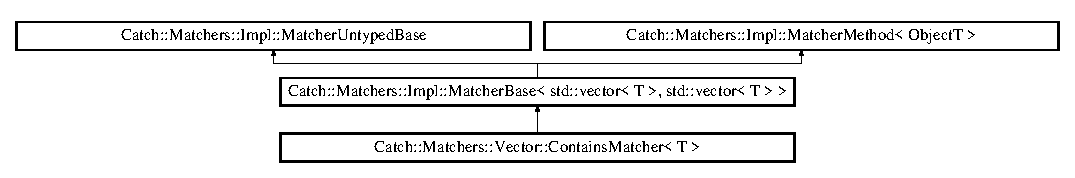
\includegraphics[height=1.944444cm]{struct_catch_1_1_matchers_1_1_vector_1_1_contains_matcher}
\end{center}
\end{figure}
\subsection*{Public Member Functions}
\begin{DoxyCompactItemize}
\item 
\mbox{\hyperlink{struct_catch_1_1_matchers_1_1_vector_1_1_contains_matcher_ad8e92c8399be6dce75bb5702cdfab700}{Contains\+Matcher}} (std\+::vector$<$ T $>$ const \&comparator)
\item 
bool \mbox{\hyperlink{struct_catch_1_1_matchers_1_1_vector_1_1_contains_matcher_aba81516816a6796124dd4fe4843e7284}{match}} (std\+::vector$<$ T $>$ const \&v) const \mbox{\hyperlink{catch_8hpp_a8ecdce4d3f57835f707915ae831eb847}{C\+A\+T\+C\+H\+\_\+\+O\+V\+E\+R\+R\+I\+DE}}
\item 
virtual std\+::string \mbox{\hyperlink{struct_catch_1_1_matchers_1_1_vector_1_1_contains_matcher_add1a31f049cec89f980424ecdb7027ac}{describe}} () const \mbox{\hyperlink{catch_8hpp_a8ecdce4d3f57835f707915ae831eb847}{C\+A\+T\+C\+H\+\_\+\+O\+V\+E\+R\+R\+I\+DE}}
\end{DoxyCompactItemize}
\subsection*{Public Attributes}
\begin{DoxyCompactItemize}
\item 
std\+::vector$<$ T $>$ const  \& \mbox{\hyperlink{struct_catch_1_1_matchers_1_1_vector_1_1_contains_matcher_a83d051166e4ed0d535219ad6ee99abb2}{m\+\_\+comparator}}
\end{DoxyCompactItemize}
\subsection*{Additional Inherited Members}


\subsection{Constructor \& Destructor Documentation}
\mbox{\Hypertarget{struct_catch_1_1_matchers_1_1_vector_1_1_contains_matcher_ad8e92c8399be6dce75bb5702cdfab700}\label{struct_catch_1_1_matchers_1_1_vector_1_1_contains_matcher_ad8e92c8399be6dce75bb5702cdfab700}} 
\index{Catch\+::\+Matchers\+::\+Vector\+::\+Contains\+Matcher@{Catch\+::\+Matchers\+::\+Vector\+::\+Contains\+Matcher}!Contains\+Matcher@{Contains\+Matcher}}
\index{Contains\+Matcher@{Contains\+Matcher}!Catch\+::\+Matchers\+::\+Vector\+::\+Contains\+Matcher@{Catch\+::\+Matchers\+::\+Vector\+::\+Contains\+Matcher}}
\subsubsection{\texorpdfstring{Contains\+Matcher()}{ContainsMatcher()}}
{\footnotesize\ttfamily template$<$typename T $>$ \\
\mbox{\hyperlink{struct_catch_1_1_matchers_1_1_vector_1_1_contains_matcher}{Catch\+::\+Matchers\+::\+Vector\+::\+Contains\+Matcher}}$<$ T $>$\+::\mbox{\hyperlink{struct_catch_1_1_matchers_1_1_vector_1_1_contains_matcher}{Contains\+Matcher}} (\begin{DoxyParamCaption}\item[{std\+::vector$<$ T $>$ const \&}]{comparator }\end{DoxyParamCaption})\hspace{0.3cm}{\ttfamily [inline]}}



\subsection{Member Function Documentation}
\mbox{\Hypertarget{struct_catch_1_1_matchers_1_1_vector_1_1_contains_matcher_add1a31f049cec89f980424ecdb7027ac}\label{struct_catch_1_1_matchers_1_1_vector_1_1_contains_matcher_add1a31f049cec89f980424ecdb7027ac}} 
\index{Catch\+::\+Matchers\+::\+Vector\+::\+Contains\+Matcher@{Catch\+::\+Matchers\+::\+Vector\+::\+Contains\+Matcher}!describe@{describe}}
\index{describe@{describe}!Catch\+::\+Matchers\+::\+Vector\+::\+Contains\+Matcher@{Catch\+::\+Matchers\+::\+Vector\+::\+Contains\+Matcher}}
\subsubsection{\texorpdfstring{describe()}{describe()}}
{\footnotesize\ttfamily template$<$typename T $>$ \\
virtual std\+::string \mbox{\hyperlink{struct_catch_1_1_matchers_1_1_vector_1_1_contains_matcher}{Catch\+::\+Matchers\+::\+Vector\+::\+Contains\+Matcher}}$<$ T $>$\+::describe (\begin{DoxyParamCaption}{ }\end{DoxyParamCaption}) const\hspace{0.3cm}{\ttfamily [inline]}, {\ttfamily [virtual]}}



Implements \mbox{\hyperlink{class_catch_1_1_matchers_1_1_impl_1_1_matcher_untyped_base_a91d3a907dbfcbb596077df24f6e11fe2}{Catch\+::\+Matchers\+::\+Impl\+::\+Matcher\+Untyped\+Base}}.

\mbox{\Hypertarget{struct_catch_1_1_matchers_1_1_vector_1_1_contains_matcher_aba81516816a6796124dd4fe4843e7284}\label{struct_catch_1_1_matchers_1_1_vector_1_1_contains_matcher_aba81516816a6796124dd4fe4843e7284}} 
\index{Catch\+::\+Matchers\+::\+Vector\+::\+Contains\+Matcher@{Catch\+::\+Matchers\+::\+Vector\+::\+Contains\+Matcher}!match@{match}}
\index{match@{match}!Catch\+::\+Matchers\+::\+Vector\+::\+Contains\+Matcher@{Catch\+::\+Matchers\+::\+Vector\+::\+Contains\+Matcher}}
\subsubsection{\texorpdfstring{match()}{match()}}
{\footnotesize\ttfamily template$<$typename T $>$ \\
bool \mbox{\hyperlink{struct_catch_1_1_matchers_1_1_vector_1_1_contains_matcher}{Catch\+::\+Matchers\+::\+Vector\+::\+Contains\+Matcher}}$<$ T $>$\+::match (\begin{DoxyParamCaption}\item[{std\+::vector$<$ T $>$ const \&}]{v }\end{DoxyParamCaption}) const\hspace{0.3cm}{\ttfamily [inline]}}



\subsection{Member Data Documentation}
\mbox{\Hypertarget{struct_catch_1_1_matchers_1_1_vector_1_1_contains_matcher_a83d051166e4ed0d535219ad6ee99abb2}\label{struct_catch_1_1_matchers_1_1_vector_1_1_contains_matcher_a83d051166e4ed0d535219ad6ee99abb2}} 
\index{Catch\+::\+Matchers\+::\+Vector\+::\+Contains\+Matcher@{Catch\+::\+Matchers\+::\+Vector\+::\+Contains\+Matcher}!m\+\_\+comparator@{m\+\_\+comparator}}
\index{m\+\_\+comparator@{m\+\_\+comparator}!Catch\+::\+Matchers\+::\+Vector\+::\+Contains\+Matcher@{Catch\+::\+Matchers\+::\+Vector\+::\+Contains\+Matcher}}
\subsubsection{\texorpdfstring{m\+\_\+comparator}{m\_comparator}}
{\footnotesize\ttfamily template$<$typename T $>$ \\
std\+::vector$<$T$>$ const\& \mbox{\hyperlink{struct_catch_1_1_matchers_1_1_vector_1_1_contains_matcher}{Catch\+::\+Matchers\+::\+Vector\+::\+Contains\+Matcher}}$<$ T $>$\+::m\+\_\+comparator}



The documentation for this struct was generated from the following file\+:\begin{DoxyCompactItemize}
\item 
include/\mbox{\hyperlink{catch_8hpp}{catch.\+hpp}}\end{DoxyCompactItemize}

\hypertarget{struct_catch_1_1_copyable_stream}{}\section{Catch\+:\+:Copyable\+Stream Struct Reference}
\label{struct_catch_1_1_copyable_stream}\index{Catch\+::\+Copyable\+Stream@{Catch\+::\+Copyable\+Stream}}


{\ttfamily \#include $<$catch.\+hpp$>$}

\subsection*{Public Member Functions}
\begin{DoxyCompactItemize}
\item 
\mbox{\hyperlink{struct_catch_1_1_copyable_stream_a5a61d0da675ae00cd46efaef4c445cdd}{Copyable\+Stream}} ()
\item 
\mbox{\hyperlink{struct_catch_1_1_copyable_stream_a0e72dc16240653f52c17106f4bf34da8}{Copyable\+Stream}} (\mbox{\hyperlink{struct_catch_1_1_copyable_stream}{Copyable\+Stream}} const \&other)
\item 
\mbox{\hyperlink{struct_catch_1_1_copyable_stream}{Copyable\+Stream}} \& \mbox{\hyperlink{struct_catch_1_1_copyable_stream_a1760fa29b38011c5845171260bec0966}{operator=}} (\mbox{\hyperlink{struct_catch_1_1_copyable_stream}{Copyable\+Stream}} const \&other)
\end{DoxyCompactItemize}
\subsection*{Public Attributes}
\begin{DoxyCompactItemize}
\item 
std\+::ostringstream \mbox{\hyperlink{struct_catch_1_1_copyable_stream_ae123fb4d673e7d7a13a3c5f6bc5d426c}{oss}}
\end{DoxyCompactItemize}


\subsection{Constructor \& Destructor Documentation}
\mbox{\Hypertarget{struct_catch_1_1_copyable_stream_a5a61d0da675ae00cd46efaef4c445cdd}\label{struct_catch_1_1_copyable_stream_a5a61d0da675ae00cd46efaef4c445cdd}} 
\index{Catch\+::\+Copyable\+Stream@{Catch\+::\+Copyable\+Stream}!Copyable\+Stream@{Copyable\+Stream}}
\index{Copyable\+Stream@{Copyable\+Stream}!Catch\+::\+Copyable\+Stream@{Catch\+::\+Copyable\+Stream}}
\subsubsection{\texorpdfstring{Copyable\+Stream()}{CopyableStream()}\hspace{0.1cm}{\footnotesize\ttfamily [1/2]}}
{\footnotesize\ttfamily Catch\+::\+Copyable\+Stream\+::\+Copyable\+Stream (\begin{DoxyParamCaption}{ }\end{DoxyParamCaption})\hspace{0.3cm}{\ttfamily [inline]}}

\mbox{\Hypertarget{struct_catch_1_1_copyable_stream_a0e72dc16240653f52c17106f4bf34da8}\label{struct_catch_1_1_copyable_stream_a0e72dc16240653f52c17106f4bf34da8}} 
\index{Catch\+::\+Copyable\+Stream@{Catch\+::\+Copyable\+Stream}!Copyable\+Stream@{Copyable\+Stream}}
\index{Copyable\+Stream@{Copyable\+Stream}!Catch\+::\+Copyable\+Stream@{Catch\+::\+Copyable\+Stream}}
\subsubsection{\texorpdfstring{Copyable\+Stream()}{CopyableStream()}\hspace{0.1cm}{\footnotesize\ttfamily [2/2]}}
{\footnotesize\ttfamily Catch\+::\+Copyable\+Stream\+::\+Copyable\+Stream (\begin{DoxyParamCaption}\item[{\mbox{\hyperlink{struct_catch_1_1_copyable_stream}{Copyable\+Stream}} const \&}]{other }\end{DoxyParamCaption})\hspace{0.3cm}{\ttfamily [inline]}}



\subsection{Member Function Documentation}
\mbox{\Hypertarget{struct_catch_1_1_copyable_stream_a1760fa29b38011c5845171260bec0966}\label{struct_catch_1_1_copyable_stream_a1760fa29b38011c5845171260bec0966}} 
\index{Catch\+::\+Copyable\+Stream@{Catch\+::\+Copyable\+Stream}!operator=@{operator=}}
\index{operator=@{operator=}!Catch\+::\+Copyable\+Stream@{Catch\+::\+Copyable\+Stream}}
\subsubsection{\texorpdfstring{operator=()}{operator=()}}
{\footnotesize\ttfamily \mbox{\hyperlink{struct_catch_1_1_copyable_stream}{Copyable\+Stream}}\& Catch\+::\+Copyable\+Stream\+::operator= (\begin{DoxyParamCaption}\item[{\mbox{\hyperlink{struct_catch_1_1_copyable_stream}{Copyable\+Stream}} const \&}]{other }\end{DoxyParamCaption})\hspace{0.3cm}{\ttfamily [inline]}}



\subsection{Member Data Documentation}
\mbox{\Hypertarget{struct_catch_1_1_copyable_stream_ae123fb4d673e7d7a13a3c5f6bc5d426c}\label{struct_catch_1_1_copyable_stream_ae123fb4d673e7d7a13a3c5f6bc5d426c}} 
\index{Catch\+::\+Copyable\+Stream@{Catch\+::\+Copyable\+Stream}!oss@{oss}}
\index{oss@{oss}!Catch\+::\+Copyable\+Stream@{Catch\+::\+Copyable\+Stream}}
\subsubsection{\texorpdfstring{oss}{oss}}
{\footnotesize\ttfamily std\+::ostringstream Catch\+::\+Copyable\+Stream\+::oss}



The documentation for this struct was generated from the following file\+:\begin{DoxyCompactItemize}
\item 
include/\mbox{\hyperlink{catch_8hpp}{catch.\+hpp}}\end{DoxyCompactItemize}

\hypertarget{struct_catch_1_1_counts}{}\section{Catch\+:\+:Counts Struct Reference}
\label{struct_catch_1_1_counts}\index{Catch\+::\+Counts@{Catch\+::\+Counts}}


{\ttfamily \#include $<$catch.\+hpp$>$}

\subsection*{Public Member Functions}
\begin{DoxyCompactItemize}
\item 
\mbox{\hyperlink{struct_catch_1_1_counts_aab9092ce70d4b0179cc743555d2fc39b}{Counts}} ()
\item 
\mbox{\hyperlink{struct_catch_1_1_counts}{Counts}} \mbox{\hyperlink{struct_catch_1_1_counts_aaa10666f559057e3e860d2a5a6fae4c4}{operator-\/}} (\mbox{\hyperlink{struct_catch_1_1_counts}{Counts}} const \&other) const
\item 
\mbox{\hyperlink{struct_catch_1_1_counts}{Counts}} \& \mbox{\hyperlink{struct_catch_1_1_counts_a322a89475cd2cc039140ef371e973677}{operator+=}} (\mbox{\hyperlink{struct_catch_1_1_counts}{Counts}} const \&other)
\item 
std\+::size\+\_\+t \mbox{\hyperlink{struct_catch_1_1_counts_a94f969c09cf52d1339c085c9603cd1d3}{total}} () const
\item 
bool \mbox{\hyperlink{struct_catch_1_1_counts_a84999490e0ecaa3de5e121bf48eda1b3}{all\+Passed}} () const
\item 
bool \mbox{\hyperlink{struct_catch_1_1_counts_a33bd996e016030155b99fe1c51c08991}{all\+Ok}} () const
\end{DoxyCompactItemize}
\subsection*{Public Attributes}
\begin{DoxyCompactItemize}
\item 
std\+::size\+\_\+t \mbox{\hyperlink{struct_catch_1_1_counts_ad28daaf3de28006400208b6dd0c631e6}{passed}}
\item 
std\+::size\+\_\+t \mbox{\hyperlink{struct_catch_1_1_counts_a19982a3817a3bc2c07f0290e71f497a3}{failed}}
\item 
std\+::size\+\_\+t \mbox{\hyperlink{struct_catch_1_1_counts_ac090973a2ff51394cd452718e75c073e}{failed\+But\+Ok}}
\end{DoxyCompactItemize}


\subsection{Constructor \& Destructor Documentation}
\mbox{\Hypertarget{struct_catch_1_1_counts_aab9092ce70d4b0179cc743555d2fc39b}\label{struct_catch_1_1_counts_aab9092ce70d4b0179cc743555d2fc39b}} 
\index{Catch\+::\+Counts@{Catch\+::\+Counts}!Counts@{Counts}}
\index{Counts@{Counts}!Catch\+::\+Counts@{Catch\+::\+Counts}}
\subsubsection{\texorpdfstring{Counts()}{Counts()}}
{\footnotesize\ttfamily Catch\+::\+Counts\+::\+Counts (\begin{DoxyParamCaption}{ }\end{DoxyParamCaption})\hspace{0.3cm}{\ttfamily [inline]}}



\subsection{Member Function Documentation}
\mbox{\Hypertarget{struct_catch_1_1_counts_a33bd996e016030155b99fe1c51c08991}\label{struct_catch_1_1_counts_a33bd996e016030155b99fe1c51c08991}} 
\index{Catch\+::\+Counts@{Catch\+::\+Counts}!all\+Ok@{all\+Ok}}
\index{all\+Ok@{all\+Ok}!Catch\+::\+Counts@{Catch\+::\+Counts}}
\subsubsection{\texorpdfstring{all\+Ok()}{allOk()}}
{\footnotesize\ttfamily bool Catch\+::\+Counts\+::all\+Ok (\begin{DoxyParamCaption}{ }\end{DoxyParamCaption}) const\hspace{0.3cm}{\ttfamily [inline]}}

\mbox{\Hypertarget{struct_catch_1_1_counts_a84999490e0ecaa3de5e121bf48eda1b3}\label{struct_catch_1_1_counts_a84999490e0ecaa3de5e121bf48eda1b3}} 
\index{Catch\+::\+Counts@{Catch\+::\+Counts}!all\+Passed@{all\+Passed}}
\index{all\+Passed@{all\+Passed}!Catch\+::\+Counts@{Catch\+::\+Counts}}
\subsubsection{\texorpdfstring{all\+Passed()}{allPassed()}}
{\footnotesize\ttfamily bool Catch\+::\+Counts\+::all\+Passed (\begin{DoxyParamCaption}{ }\end{DoxyParamCaption}) const\hspace{0.3cm}{\ttfamily [inline]}}

\mbox{\Hypertarget{struct_catch_1_1_counts_a322a89475cd2cc039140ef371e973677}\label{struct_catch_1_1_counts_a322a89475cd2cc039140ef371e973677}} 
\index{Catch\+::\+Counts@{Catch\+::\+Counts}!operator+=@{operator+=}}
\index{operator+=@{operator+=}!Catch\+::\+Counts@{Catch\+::\+Counts}}
\subsubsection{\texorpdfstring{operator+=()}{operator+=()}}
{\footnotesize\ttfamily \mbox{\hyperlink{struct_catch_1_1_counts}{Counts}}\& Catch\+::\+Counts\+::operator+= (\begin{DoxyParamCaption}\item[{\mbox{\hyperlink{struct_catch_1_1_counts}{Counts}} const \&}]{other }\end{DoxyParamCaption})\hspace{0.3cm}{\ttfamily [inline]}}

\mbox{\Hypertarget{struct_catch_1_1_counts_aaa10666f559057e3e860d2a5a6fae4c4}\label{struct_catch_1_1_counts_aaa10666f559057e3e860d2a5a6fae4c4}} 
\index{Catch\+::\+Counts@{Catch\+::\+Counts}!operator-\/@{operator-\/}}
\index{operator-\/@{operator-\/}!Catch\+::\+Counts@{Catch\+::\+Counts}}
\subsubsection{\texorpdfstring{operator-\/()}{operator-()}}
{\footnotesize\ttfamily \mbox{\hyperlink{struct_catch_1_1_counts}{Counts}} Catch\+::\+Counts\+::operator-\/ (\begin{DoxyParamCaption}\item[{\mbox{\hyperlink{struct_catch_1_1_counts}{Counts}} const \&}]{other }\end{DoxyParamCaption}) const\hspace{0.3cm}{\ttfamily [inline]}}

\mbox{\Hypertarget{struct_catch_1_1_counts_a94f969c09cf52d1339c085c9603cd1d3}\label{struct_catch_1_1_counts_a94f969c09cf52d1339c085c9603cd1d3}} 
\index{Catch\+::\+Counts@{Catch\+::\+Counts}!total@{total}}
\index{total@{total}!Catch\+::\+Counts@{Catch\+::\+Counts}}
\subsubsection{\texorpdfstring{total()}{total()}}
{\footnotesize\ttfamily std\+::size\+\_\+t Catch\+::\+Counts\+::total (\begin{DoxyParamCaption}{ }\end{DoxyParamCaption}) const\hspace{0.3cm}{\ttfamily [inline]}}



\subsection{Member Data Documentation}
\mbox{\Hypertarget{struct_catch_1_1_counts_a19982a3817a3bc2c07f0290e71f497a3}\label{struct_catch_1_1_counts_a19982a3817a3bc2c07f0290e71f497a3}} 
\index{Catch\+::\+Counts@{Catch\+::\+Counts}!failed@{failed}}
\index{failed@{failed}!Catch\+::\+Counts@{Catch\+::\+Counts}}
\subsubsection{\texorpdfstring{failed}{failed}}
{\footnotesize\ttfamily std\+::size\+\_\+t Catch\+::\+Counts\+::failed}

\mbox{\Hypertarget{struct_catch_1_1_counts_ac090973a2ff51394cd452718e75c073e}\label{struct_catch_1_1_counts_ac090973a2ff51394cd452718e75c073e}} 
\index{Catch\+::\+Counts@{Catch\+::\+Counts}!failed\+But\+Ok@{failed\+But\+Ok}}
\index{failed\+But\+Ok@{failed\+But\+Ok}!Catch\+::\+Counts@{Catch\+::\+Counts}}
\subsubsection{\texorpdfstring{failed\+But\+Ok}{failedButOk}}
{\footnotesize\ttfamily std\+::size\+\_\+t Catch\+::\+Counts\+::failed\+But\+Ok}

\mbox{\Hypertarget{struct_catch_1_1_counts_ad28daaf3de28006400208b6dd0c631e6}\label{struct_catch_1_1_counts_ad28daaf3de28006400208b6dd0c631e6}} 
\index{Catch\+::\+Counts@{Catch\+::\+Counts}!passed@{passed}}
\index{passed@{passed}!Catch\+::\+Counts@{Catch\+::\+Counts}}
\subsubsection{\texorpdfstring{passed}{passed}}
{\footnotesize\ttfamily std\+::size\+\_\+t Catch\+::\+Counts\+::passed}



The documentation for this struct was generated from the following file\+:\begin{DoxyCompactItemize}
\item 
include/\mbox{\hyperlink{catch_8hpp}{catch.\+hpp}}\end{DoxyCompactItemize}

\hypertarget{struct_catch_1_1_decomposed_expression}{}\section{Catch\+:\+:Decomposed\+Expression Struct Reference}
\label{struct_catch_1_1_decomposed_expression}\index{Catch\+::\+Decomposed\+Expression@{Catch\+::\+Decomposed\+Expression}}


{\ttfamily \#include $<$catch.\+hpp$>$}

Inheritance diagram for Catch\+:\+:Decomposed\+Expression\+:\begin{figure}[H]
\begin{center}
\leavevmode
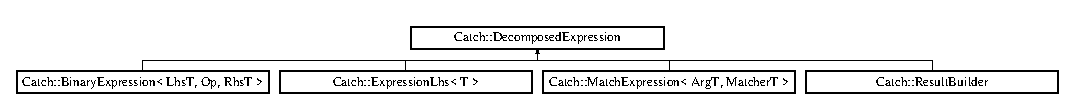
\includegraphics[height=1.029412cm]{struct_catch_1_1_decomposed_expression}
\end{center}
\end{figure}
\subsection*{Public Member Functions}
\begin{DoxyCompactItemize}
\item 
virtual \mbox{\hyperlink{struct_catch_1_1_decomposed_expression_aa627c69bd83582c33a4d4dcac403936c}{$\sim$\+Decomposed\+Expression}} ()
\item 
virtual bool \mbox{\hyperlink{struct_catch_1_1_decomposed_expression_a1c458ece47b71f093290dbdf9bb31fdb}{is\+Binary\+Expression}} () const
\item 
virtual void \mbox{\hyperlink{struct_catch_1_1_decomposed_expression_a9ce7f356dc96f11f80e40c82f5aa7e55}{reconstruct\+Expression}} (std\+::string \&dest) const =0
\item 
{\footnotesize template$<$typename T $>$ }\\S\+T\+A\+T\+I\+C\+\_\+\+A\+S\+S\+E\+R\+T\+\_\+\+Expression\+\_\+\+Too\+\_\+\+Complex\+\_\+\+Please\+\_\+\+Rewrite\+\_\+\+As\+\_\+\+Binary\+\_\+\+Comparison \& \mbox{\hyperlink{struct_catch_1_1_decomposed_expression_aa2ce96ce31fef4afb21861bc0276edb9}{operator+}} (T const \&)
\item 
{\footnotesize template$<$typename T $>$ }\\S\+T\+A\+T\+I\+C\+\_\+\+A\+S\+S\+E\+R\+T\+\_\+\+Expression\+\_\+\+Too\+\_\+\+Complex\+\_\+\+Please\+\_\+\+Rewrite\+\_\+\+As\+\_\+\+Binary\+\_\+\+Comparison \& \mbox{\hyperlink{struct_catch_1_1_decomposed_expression_aff39fb5d060abbd018c83b998d32c366}{operator-\/}} (T const \&)
\item 
{\footnotesize template$<$typename T $>$ }\\S\+T\+A\+T\+I\+C\+\_\+\+A\+S\+S\+E\+R\+T\+\_\+\+Expression\+\_\+\+Too\+\_\+\+Complex\+\_\+\+Please\+\_\+\+Rewrite\+\_\+\+As\+\_\+\+Binary\+\_\+\+Comparison \& \mbox{\hyperlink{struct_catch_1_1_decomposed_expression_afb5527e8e3cb8edca5113ec9801249d8}{operator$\ast$}} (T const \&)
\item 
{\footnotesize template$<$typename T $>$ }\\S\+T\+A\+T\+I\+C\+\_\+\+A\+S\+S\+E\+R\+T\+\_\+\+Expression\+\_\+\+Too\+\_\+\+Complex\+\_\+\+Please\+\_\+\+Rewrite\+\_\+\+As\+\_\+\+Binary\+\_\+\+Comparison \& \mbox{\hyperlink{struct_catch_1_1_decomposed_expression_a519d7e2363a92106e46371c9c04044a7}{operator/}} (T const \&)
\item 
{\footnotesize template$<$typename T $>$ }\\S\+T\+A\+T\+I\+C\+\_\+\+A\+S\+S\+E\+R\+T\+\_\+\+Expression\+\_\+\+Too\+\_\+\+Complex\+\_\+\+Please\+\_\+\+Rewrite\+\_\+\+As\+\_\+\+Binary\+\_\+\+Comparison \& \mbox{\hyperlink{struct_catch_1_1_decomposed_expression_a6584335aadaee847c9d06ca8f13a4477}{operator\%}} (T const \&)
\item 
{\footnotesize template$<$typename T $>$ }\\S\+T\+A\+T\+I\+C\+\_\+\+A\+S\+S\+E\+R\+T\+\_\+\+Expression\+\_\+\+Too\+\_\+\+Complex\+\_\+\+Please\+\_\+\+Rewrite\+\_\+\+As\+\_\+\+Binary\+\_\+\+Comparison \& \mbox{\hyperlink{struct_catch_1_1_decomposed_expression_a14d913535796145b39101a16c0c490da}{operator\&\&}} (T const \&)
\item 
{\footnotesize template$<$typename T $>$ }\\S\+T\+A\+T\+I\+C\+\_\+\+A\+S\+S\+E\+R\+T\+\_\+\+Expression\+\_\+\+Too\+\_\+\+Complex\+\_\+\+Please\+\_\+\+Rewrite\+\_\+\+As\+\_\+\+Binary\+\_\+\+Comparison \& \mbox{\hyperlink{struct_catch_1_1_decomposed_expression_ab4800d277290088fea9c594cfdd4f1c7}{operator$\vert$$\vert$}} (T const \&)
\end{DoxyCompactItemize}


\subsection{Constructor \& Destructor Documentation}
\mbox{\Hypertarget{struct_catch_1_1_decomposed_expression_aa627c69bd83582c33a4d4dcac403936c}\label{struct_catch_1_1_decomposed_expression_aa627c69bd83582c33a4d4dcac403936c}} 
\index{Catch\+::\+Decomposed\+Expression@{Catch\+::\+Decomposed\+Expression}!````~Decomposed\+Expression@{$\sim$\+Decomposed\+Expression}}
\index{````~Decomposed\+Expression@{$\sim$\+Decomposed\+Expression}!Catch\+::\+Decomposed\+Expression@{Catch\+::\+Decomposed\+Expression}}
\subsubsection{\texorpdfstring{$\sim$\+Decomposed\+Expression()}{~DecomposedExpression()}}
{\footnotesize\ttfamily virtual Catch\+::\+Decomposed\+Expression\+::$\sim$\+Decomposed\+Expression (\begin{DoxyParamCaption}{ }\end{DoxyParamCaption})\hspace{0.3cm}{\ttfamily [inline]}, {\ttfamily [virtual]}}



\subsection{Member Function Documentation}
\mbox{\Hypertarget{struct_catch_1_1_decomposed_expression_a1c458ece47b71f093290dbdf9bb31fdb}\label{struct_catch_1_1_decomposed_expression_a1c458ece47b71f093290dbdf9bb31fdb}} 
\index{Catch\+::\+Decomposed\+Expression@{Catch\+::\+Decomposed\+Expression}!is\+Binary\+Expression@{is\+Binary\+Expression}}
\index{is\+Binary\+Expression@{is\+Binary\+Expression}!Catch\+::\+Decomposed\+Expression@{Catch\+::\+Decomposed\+Expression}}
\subsubsection{\texorpdfstring{is\+Binary\+Expression()}{isBinaryExpression()}}
{\footnotesize\ttfamily virtual bool Catch\+::\+Decomposed\+Expression\+::is\+Binary\+Expression (\begin{DoxyParamCaption}{ }\end{DoxyParamCaption}) const\hspace{0.3cm}{\ttfamily [inline]}, {\ttfamily [virtual]}}



Reimplemented in \mbox{\hyperlink{class_catch_1_1_match_expression_ac4edf6e9a6e5762a487db1486d0d1f45}{Catch\+::\+Match\+Expression$<$ Arg\+T, Matcher\+T $>$}}, and \mbox{\hyperlink{class_catch_1_1_binary_expression_a4c617c0b6a73a9cafbbf900909c7c258}{Catch\+::\+Binary\+Expression$<$ Lhs\+T, Op, Rhs\+T $>$}}.

\mbox{\Hypertarget{struct_catch_1_1_decomposed_expression_a6584335aadaee847c9d06ca8f13a4477}\label{struct_catch_1_1_decomposed_expression_a6584335aadaee847c9d06ca8f13a4477}} 
\index{Catch\+::\+Decomposed\+Expression@{Catch\+::\+Decomposed\+Expression}!operator\%@{operator\%}}
\index{operator\%@{operator\%}!Catch\+::\+Decomposed\+Expression@{Catch\+::\+Decomposed\+Expression}}
\subsubsection{\texorpdfstring{operator\%()}{operator\%()}}
{\footnotesize\ttfamily template$<$typename T $>$ \\
S\+T\+A\+T\+I\+C\+\_\+\+A\+S\+S\+E\+R\+T\+\_\+\+Expression\+\_\+\+Too\+\_\+\+Complex\+\_\+\+Please\+\_\+\+Rewrite\+\_\+\+As\+\_\+\+Binary\+\_\+\+Comparison\& Catch\+::\+Decomposed\+Expression\+::operator\% (\begin{DoxyParamCaption}\item[{T const \&}]{ }\end{DoxyParamCaption})}

\mbox{\Hypertarget{struct_catch_1_1_decomposed_expression_a14d913535796145b39101a16c0c490da}\label{struct_catch_1_1_decomposed_expression_a14d913535796145b39101a16c0c490da}} 
\index{Catch\+::\+Decomposed\+Expression@{Catch\+::\+Decomposed\+Expression}!operator\&\&@{operator\&\&}}
\index{operator\&\&@{operator\&\&}!Catch\+::\+Decomposed\+Expression@{Catch\+::\+Decomposed\+Expression}}
\subsubsection{\texorpdfstring{operator\&\&()}{operator\&\&()}}
{\footnotesize\ttfamily template$<$typename T $>$ \\
S\+T\+A\+T\+I\+C\+\_\+\+A\+S\+S\+E\+R\+T\+\_\+\+Expression\+\_\+\+Too\+\_\+\+Complex\+\_\+\+Please\+\_\+\+Rewrite\+\_\+\+As\+\_\+\+Binary\+\_\+\+Comparison\& Catch\+::\+Decomposed\+Expression\+::operator \&\& (\begin{DoxyParamCaption}\item[{T const \&}]{ }\end{DoxyParamCaption})}

\mbox{\Hypertarget{struct_catch_1_1_decomposed_expression_afb5527e8e3cb8edca5113ec9801249d8}\label{struct_catch_1_1_decomposed_expression_afb5527e8e3cb8edca5113ec9801249d8}} 
\index{Catch\+::\+Decomposed\+Expression@{Catch\+::\+Decomposed\+Expression}!operator$\ast$@{operator$\ast$}}
\index{operator$\ast$@{operator$\ast$}!Catch\+::\+Decomposed\+Expression@{Catch\+::\+Decomposed\+Expression}}
\subsubsection{\texorpdfstring{operator$\ast$()}{operator*()}}
{\footnotesize\ttfamily template$<$typename T $>$ \\
S\+T\+A\+T\+I\+C\+\_\+\+A\+S\+S\+E\+R\+T\+\_\+\+Expression\+\_\+\+Too\+\_\+\+Complex\+\_\+\+Please\+\_\+\+Rewrite\+\_\+\+As\+\_\+\+Binary\+\_\+\+Comparison\& Catch\+::\+Decomposed\+Expression\+::operator$\ast$ (\begin{DoxyParamCaption}\item[{T const \&}]{ }\end{DoxyParamCaption})}

\mbox{\Hypertarget{struct_catch_1_1_decomposed_expression_aa2ce96ce31fef4afb21861bc0276edb9}\label{struct_catch_1_1_decomposed_expression_aa2ce96ce31fef4afb21861bc0276edb9}} 
\index{Catch\+::\+Decomposed\+Expression@{Catch\+::\+Decomposed\+Expression}!operator+@{operator+}}
\index{operator+@{operator+}!Catch\+::\+Decomposed\+Expression@{Catch\+::\+Decomposed\+Expression}}
\subsubsection{\texorpdfstring{operator+()}{operator+()}}
{\footnotesize\ttfamily template$<$typename T $>$ \\
S\+T\+A\+T\+I\+C\+\_\+\+A\+S\+S\+E\+R\+T\+\_\+\+Expression\+\_\+\+Too\+\_\+\+Complex\+\_\+\+Please\+\_\+\+Rewrite\+\_\+\+As\+\_\+\+Binary\+\_\+\+Comparison\& Catch\+::\+Decomposed\+Expression\+::operator+ (\begin{DoxyParamCaption}\item[{T const \&}]{ }\end{DoxyParamCaption})}

\mbox{\Hypertarget{struct_catch_1_1_decomposed_expression_aff39fb5d060abbd018c83b998d32c366}\label{struct_catch_1_1_decomposed_expression_aff39fb5d060abbd018c83b998d32c366}} 
\index{Catch\+::\+Decomposed\+Expression@{Catch\+::\+Decomposed\+Expression}!operator-\/@{operator-\/}}
\index{operator-\/@{operator-\/}!Catch\+::\+Decomposed\+Expression@{Catch\+::\+Decomposed\+Expression}}
\subsubsection{\texorpdfstring{operator-\/()}{operator-()}}
{\footnotesize\ttfamily template$<$typename T $>$ \\
S\+T\+A\+T\+I\+C\+\_\+\+A\+S\+S\+E\+R\+T\+\_\+\+Expression\+\_\+\+Too\+\_\+\+Complex\+\_\+\+Please\+\_\+\+Rewrite\+\_\+\+As\+\_\+\+Binary\+\_\+\+Comparison\& Catch\+::\+Decomposed\+Expression\+::operator-\/ (\begin{DoxyParamCaption}\item[{T const \&}]{ }\end{DoxyParamCaption})}

\mbox{\Hypertarget{struct_catch_1_1_decomposed_expression_a519d7e2363a92106e46371c9c04044a7}\label{struct_catch_1_1_decomposed_expression_a519d7e2363a92106e46371c9c04044a7}} 
\index{Catch\+::\+Decomposed\+Expression@{Catch\+::\+Decomposed\+Expression}!operator/@{operator/}}
\index{operator/@{operator/}!Catch\+::\+Decomposed\+Expression@{Catch\+::\+Decomposed\+Expression}}
\subsubsection{\texorpdfstring{operator/()}{operator/()}}
{\footnotesize\ttfamily template$<$typename T $>$ \\
S\+T\+A\+T\+I\+C\+\_\+\+A\+S\+S\+E\+R\+T\+\_\+\+Expression\+\_\+\+Too\+\_\+\+Complex\+\_\+\+Please\+\_\+\+Rewrite\+\_\+\+As\+\_\+\+Binary\+\_\+\+Comparison\& Catch\+::\+Decomposed\+Expression\+::operator/ (\begin{DoxyParamCaption}\item[{T const \&}]{ }\end{DoxyParamCaption})}

\mbox{\Hypertarget{struct_catch_1_1_decomposed_expression_ab4800d277290088fea9c594cfdd4f1c7}\label{struct_catch_1_1_decomposed_expression_ab4800d277290088fea9c594cfdd4f1c7}} 
\index{Catch\+::\+Decomposed\+Expression@{Catch\+::\+Decomposed\+Expression}!operator\texttt{"|}\texttt{"|}@{operator\texttt{"|}\texttt{"|}}}
\index{operator\texttt{"|}\texttt{"|}@{operator\texttt{"|}\texttt{"|}}!Catch\+::\+Decomposed\+Expression@{Catch\+::\+Decomposed\+Expression}}
\subsubsection{\texorpdfstring{operator\texttt{"|}\texttt{"|}()}{operator||()}}
{\footnotesize\ttfamily template$<$typename T $>$ \\
S\+T\+A\+T\+I\+C\+\_\+\+A\+S\+S\+E\+R\+T\+\_\+\+Expression\+\_\+\+Too\+\_\+\+Complex\+\_\+\+Please\+\_\+\+Rewrite\+\_\+\+As\+\_\+\+Binary\+\_\+\+Comparison\& Catch\+::\+Decomposed\+Expression\+::operator$\vert$$\vert$ (\begin{DoxyParamCaption}\item[{T const \&}]{ }\end{DoxyParamCaption})}

\mbox{\Hypertarget{struct_catch_1_1_decomposed_expression_a9ce7f356dc96f11f80e40c82f5aa7e55}\label{struct_catch_1_1_decomposed_expression_a9ce7f356dc96f11f80e40c82f5aa7e55}} 
\index{Catch\+::\+Decomposed\+Expression@{Catch\+::\+Decomposed\+Expression}!reconstruct\+Expression@{reconstruct\+Expression}}
\index{reconstruct\+Expression@{reconstruct\+Expression}!Catch\+::\+Decomposed\+Expression@{Catch\+::\+Decomposed\+Expression}}
\subsubsection{\texorpdfstring{reconstruct\+Expression()}{reconstructExpression()}}
{\footnotesize\ttfamily virtual void Catch\+::\+Decomposed\+Expression\+::reconstruct\+Expression (\begin{DoxyParamCaption}\item[{std\+::string \&}]{dest }\end{DoxyParamCaption}) const\hspace{0.3cm}{\ttfamily [pure virtual]}}



Implemented in \mbox{\hyperlink{class_catch_1_1_match_expression_a4410a93bc5b8241eb2502f400fce7ec4}{Catch\+::\+Match\+Expression$<$ Arg\+T, Matcher\+T $>$}}, \mbox{\hyperlink{class_catch_1_1_binary_expression_a6ed73ff9af9c229f9fa3d35d019f9e37}{Catch\+::\+Binary\+Expression$<$ Lhs\+T, Op, Rhs\+T $>$}}, \mbox{\hyperlink{class_catch_1_1_expression_lhs_a7684a053e8e88a4be475a536252630da}{Catch\+::\+Expression\+Lhs$<$ T $>$}}, and \mbox{\hyperlink{class_catch_1_1_result_builder_a7d94b15cf04301a8617e7b16158b5d82}{Catch\+::\+Result\+Builder}}.



The documentation for this struct was generated from the following file\+:\begin{DoxyCompactItemize}
\item 
include/\mbox{\hyperlink{catch_8hpp}{catch.\+hpp}}\end{DoxyCompactItemize}

\hypertarget{struct_catch_1_1_matchers_1_1_std_string_1_1_ends_with_matcher}{}\section{Catch\+:\+:Matchers\+:\+:Std\+String\+:\+:Ends\+With\+Matcher Struct Reference}
\label{struct_catch_1_1_matchers_1_1_std_string_1_1_ends_with_matcher}\index{Catch\+::\+Matchers\+::\+Std\+String\+::\+Ends\+With\+Matcher@{Catch\+::\+Matchers\+::\+Std\+String\+::\+Ends\+With\+Matcher}}


{\ttfamily \#include $<$catch.\+hpp$>$}

Inheritance diagram for Catch\+:\+:Matchers\+:\+:Std\+String\+:\+:Ends\+With\+Matcher\+:\begin{figure}[H]
\begin{center}
\leavevmode
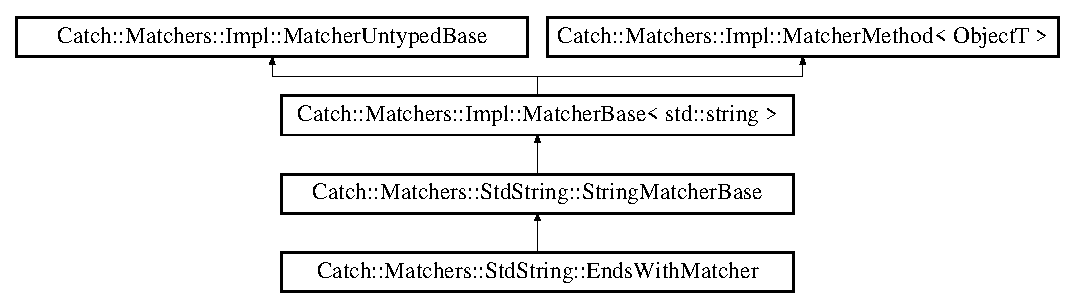
\includegraphics[height=3.696370cm]{struct_catch_1_1_matchers_1_1_std_string_1_1_ends_with_matcher}
\end{center}
\end{figure}
\subsection*{Public Member Functions}
\begin{DoxyCompactItemize}
\item 
\mbox{\hyperlink{struct_catch_1_1_matchers_1_1_std_string_1_1_ends_with_matcher_aa5ec700b4629562f74f362080accfd7b}{Ends\+With\+Matcher}} (\mbox{\hyperlink{struct_catch_1_1_matchers_1_1_std_string_1_1_cased_string}{Cased\+String}} const \&comparator)
\item 
virtual bool \mbox{\hyperlink{struct_catch_1_1_matchers_1_1_std_string_1_1_ends_with_matcher_a21c6dc68e30716d5c718f4f8c3186af1}{match}} (std\+::string const \&source) const \mbox{\hyperlink{catch_8hpp_a8ecdce4d3f57835f707915ae831eb847}{C\+A\+T\+C\+H\+\_\+\+O\+V\+E\+R\+R\+I\+DE}}
\end{DoxyCompactItemize}
\subsection*{Additional Inherited Members}


\subsection{Constructor \& Destructor Documentation}
\mbox{\Hypertarget{struct_catch_1_1_matchers_1_1_std_string_1_1_ends_with_matcher_aa5ec700b4629562f74f362080accfd7b}\label{struct_catch_1_1_matchers_1_1_std_string_1_1_ends_with_matcher_aa5ec700b4629562f74f362080accfd7b}} 
\index{Catch\+::\+Matchers\+::\+Std\+String\+::\+Ends\+With\+Matcher@{Catch\+::\+Matchers\+::\+Std\+String\+::\+Ends\+With\+Matcher}!Ends\+With\+Matcher@{Ends\+With\+Matcher}}
\index{Ends\+With\+Matcher@{Ends\+With\+Matcher}!Catch\+::\+Matchers\+::\+Std\+String\+::\+Ends\+With\+Matcher@{Catch\+::\+Matchers\+::\+Std\+String\+::\+Ends\+With\+Matcher}}
\subsubsection{\texorpdfstring{Ends\+With\+Matcher()}{EndsWithMatcher()}}
{\footnotesize\ttfamily Catch\+::\+Matchers\+::\+Std\+String\+::\+Ends\+With\+Matcher\+::\+Ends\+With\+Matcher (\begin{DoxyParamCaption}\item[{\mbox{\hyperlink{struct_catch_1_1_matchers_1_1_std_string_1_1_cased_string}{Cased\+String}} const \&}]{comparator }\end{DoxyParamCaption})}



\subsection{Member Function Documentation}
\mbox{\Hypertarget{struct_catch_1_1_matchers_1_1_std_string_1_1_ends_with_matcher_a21c6dc68e30716d5c718f4f8c3186af1}\label{struct_catch_1_1_matchers_1_1_std_string_1_1_ends_with_matcher_a21c6dc68e30716d5c718f4f8c3186af1}} 
\index{Catch\+::\+Matchers\+::\+Std\+String\+::\+Ends\+With\+Matcher@{Catch\+::\+Matchers\+::\+Std\+String\+::\+Ends\+With\+Matcher}!match@{match}}
\index{match@{match}!Catch\+::\+Matchers\+::\+Std\+String\+::\+Ends\+With\+Matcher@{Catch\+::\+Matchers\+::\+Std\+String\+::\+Ends\+With\+Matcher}}
\subsubsection{\texorpdfstring{match()}{match()}}
{\footnotesize\ttfamily virtual bool Catch\+::\+Matchers\+::\+Std\+String\+::\+Ends\+With\+Matcher\+::match (\begin{DoxyParamCaption}\item[{std\+::string const \&}]{source }\end{DoxyParamCaption}) const\hspace{0.3cm}{\ttfamily [virtual]}}



The documentation for this struct was generated from the following file\+:\begin{DoxyCompactItemize}
\item 
include/\mbox{\hyperlink{catch_8hpp}{catch.\+hpp}}\end{DoxyCompactItemize}

\hypertarget{struct_catch_1_1_matchers_1_1_std_string_1_1_equals_matcher}{}\section{Catch\+:\+:Matchers\+:\+:Std\+String\+:\+:Equals\+Matcher Struct Reference}
\label{struct_catch_1_1_matchers_1_1_std_string_1_1_equals_matcher}\index{Catch\+::\+Matchers\+::\+Std\+String\+::\+Equals\+Matcher@{Catch\+::\+Matchers\+::\+Std\+String\+::\+Equals\+Matcher}}


{\ttfamily \#include $<$catch.\+hpp$>$}

Inheritance diagram for Catch\+:\+:Matchers\+:\+:Std\+String\+:\+:Equals\+Matcher\+:\begin{figure}[H]
\begin{center}
\leavevmode
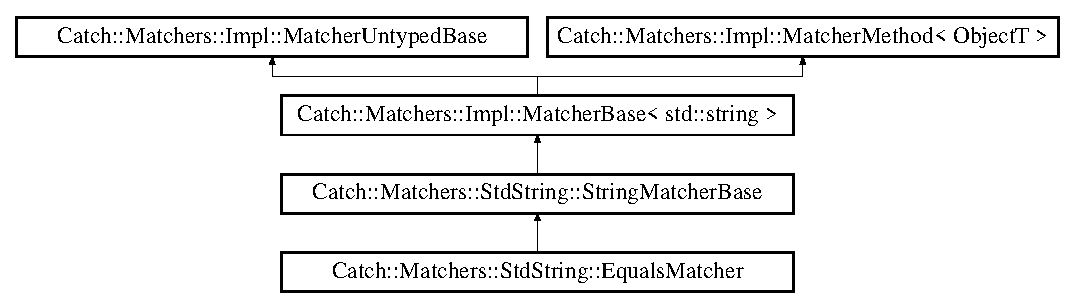
\includegraphics[height=3.696370cm]{struct_catch_1_1_matchers_1_1_std_string_1_1_equals_matcher}
\end{center}
\end{figure}
\subsection*{Public Member Functions}
\begin{DoxyCompactItemize}
\item 
\mbox{\hyperlink{struct_catch_1_1_matchers_1_1_std_string_1_1_equals_matcher_ab740f1fb2310e9fe3fed5134d4c7e4c8}{Equals\+Matcher}} (\mbox{\hyperlink{struct_catch_1_1_matchers_1_1_std_string_1_1_cased_string}{Cased\+String}} const \&comparator)
\item 
virtual bool \mbox{\hyperlink{struct_catch_1_1_matchers_1_1_std_string_1_1_equals_matcher_a2aeaac3c0efb8422643cd1b155256213}{match}} (std\+::string const \&source) const \mbox{\hyperlink{catch_8hpp_a8ecdce4d3f57835f707915ae831eb847}{C\+A\+T\+C\+H\+\_\+\+O\+V\+E\+R\+R\+I\+DE}}
\end{DoxyCompactItemize}
\subsection*{Additional Inherited Members}


\subsection{Constructor \& Destructor Documentation}
\mbox{\Hypertarget{struct_catch_1_1_matchers_1_1_std_string_1_1_equals_matcher_ab740f1fb2310e9fe3fed5134d4c7e4c8}\label{struct_catch_1_1_matchers_1_1_std_string_1_1_equals_matcher_ab740f1fb2310e9fe3fed5134d4c7e4c8}} 
\index{Catch\+::\+Matchers\+::\+Std\+String\+::\+Equals\+Matcher@{Catch\+::\+Matchers\+::\+Std\+String\+::\+Equals\+Matcher}!Equals\+Matcher@{Equals\+Matcher}}
\index{Equals\+Matcher@{Equals\+Matcher}!Catch\+::\+Matchers\+::\+Std\+String\+::\+Equals\+Matcher@{Catch\+::\+Matchers\+::\+Std\+String\+::\+Equals\+Matcher}}
\subsubsection{\texorpdfstring{Equals\+Matcher()}{EqualsMatcher()}}
{\footnotesize\ttfamily Catch\+::\+Matchers\+::\+Std\+String\+::\+Equals\+Matcher\+::\+Equals\+Matcher (\begin{DoxyParamCaption}\item[{\mbox{\hyperlink{struct_catch_1_1_matchers_1_1_std_string_1_1_cased_string}{Cased\+String}} const \&}]{comparator }\end{DoxyParamCaption})}



\subsection{Member Function Documentation}
\mbox{\Hypertarget{struct_catch_1_1_matchers_1_1_std_string_1_1_equals_matcher_a2aeaac3c0efb8422643cd1b155256213}\label{struct_catch_1_1_matchers_1_1_std_string_1_1_equals_matcher_a2aeaac3c0efb8422643cd1b155256213}} 
\index{Catch\+::\+Matchers\+::\+Std\+String\+::\+Equals\+Matcher@{Catch\+::\+Matchers\+::\+Std\+String\+::\+Equals\+Matcher}!match@{match}}
\index{match@{match}!Catch\+::\+Matchers\+::\+Std\+String\+::\+Equals\+Matcher@{Catch\+::\+Matchers\+::\+Std\+String\+::\+Equals\+Matcher}}
\subsubsection{\texorpdfstring{match()}{match()}}
{\footnotesize\ttfamily virtual bool Catch\+::\+Matchers\+::\+Std\+String\+::\+Equals\+Matcher\+::match (\begin{DoxyParamCaption}\item[{std\+::string const \&}]{source }\end{DoxyParamCaption}) const\hspace{0.3cm}{\ttfamily [virtual]}}



The documentation for this struct was generated from the following file\+:\begin{DoxyCompactItemize}
\item 
include/\mbox{\hyperlink{catch_8hpp}{catch.\+hpp}}\end{DoxyCompactItemize}

\hypertarget{struct_catch_1_1_matchers_1_1_vector_1_1_equals_matcher}{}\section{Catch\+:\+:Matchers\+:\+:Vector\+:\+:Equals\+Matcher$<$ T $>$ Struct Template Reference}
\label{struct_catch_1_1_matchers_1_1_vector_1_1_equals_matcher}\index{Catch\+::\+Matchers\+::\+Vector\+::\+Equals\+Matcher$<$ T $>$@{Catch\+::\+Matchers\+::\+Vector\+::\+Equals\+Matcher$<$ T $>$}}


{\ttfamily \#include $<$catch.\+hpp$>$}

Inheritance diagram for Catch\+:\+:Matchers\+:\+:Vector\+:\+:Equals\+Matcher$<$ T $>$\+:\begin{figure}[H]
\begin{center}
\leavevmode
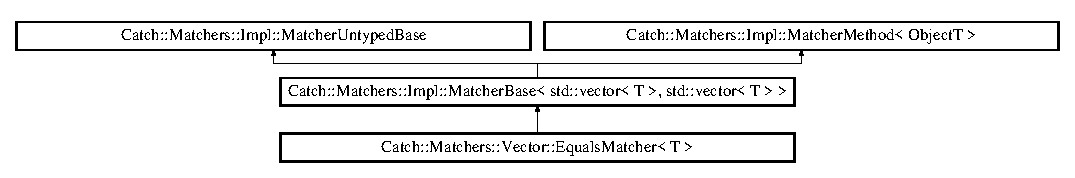
\includegraphics[height=1.944444cm]{struct_catch_1_1_matchers_1_1_vector_1_1_equals_matcher}
\end{center}
\end{figure}
\subsection*{Public Member Functions}
\begin{DoxyCompactItemize}
\item 
\mbox{\hyperlink{struct_catch_1_1_matchers_1_1_vector_1_1_equals_matcher_a3846c47780d1991dcfe87aefded98008}{Equals\+Matcher}} (std\+::vector$<$ T $>$ const \&comparator)
\item 
bool \mbox{\hyperlink{struct_catch_1_1_matchers_1_1_vector_1_1_equals_matcher_aca444c319d1b4c6f538faf9c4735da04}{match}} (std\+::vector$<$ T $>$ const \&v) const \mbox{\hyperlink{catch_8hpp_a8ecdce4d3f57835f707915ae831eb847}{C\+A\+T\+C\+H\+\_\+\+O\+V\+E\+R\+R\+I\+DE}}
\item 
virtual std\+::string \mbox{\hyperlink{struct_catch_1_1_matchers_1_1_vector_1_1_equals_matcher_aca79ade26f4a75b2a57005067e086e35}{describe}} () const \mbox{\hyperlink{catch_8hpp_a8ecdce4d3f57835f707915ae831eb847}{C\+A\+T\+C\+H\+\_\+\+O\+V\+E\+R\+R\+I\+DE}}
\end{DoxyCompactItemize}
\subsection*{Public Attributes}
\begin{DoxyCompactItemize}
\item 
std\+::vector$<$ T $>$ const  \& \mbox{\hyperlink{struct_catch_1_1_matchers_1_1_vector_1_1_equals_matcher_a56f7aa6f110a12b1b9aeb0cabbc9d755}{m\+\_\+comparator}}
\end{DoxyCompactItemize}
\subsection*{Additional Inherited Members}


\subsection{Constructor \& Destructor Documentation}
\mbox{\Hypertarget{struct_catch_1_1_matchers_1_1_vector_1_1_equals_matcher_a3846c47780d1991dcfe87aefded98008}\label{struct_catch_1_1_matchers_1_1_vector_1_1_equals_matcher_a3846c47780d1991dcfe87aefded98008}} 
\index{Catch\+::\+Matchers\+::\+Vector\+::\+Equals\+Matcher@{Catch\+::\+Matchers\+::\+Vector\+::\+Equals\+Matcher}!Equals\+Matcher@{Equals\+Matcher}}
\index{Equals\+Matcher@{Equals\+Matcher}!Catch\+::\+Matchers\+::\+Vector\+::\+Equals\+Matcher@{Catch\+::\+Matchers\+::\+Vector\+::\+Equals\+Matcher}}
\subsubsection{\texorpdfstring{Equals\+Matcher()}{EqualsMatcher()}}
{\footnotesize\ttfamily template$<$typename T $>$ \\
\mbox{\hyperlink{struct_catch_1_1_matchers_1_1_vector_1_1_equals_matcher}{Catch\+::\+Matchers\+::\+Vector\+::\+Equals\+Matcher}}$<$ T $>$\+::\mbox{\hyperlink{struct_catch_1_1_matchers_1_1_vector_1_1_equals_matcher}{Equals\+Matcher}} (\begin{DoxyParamCaption}\item[{std\+::vector$<$ T $>$ const \&}]{comparator }\end{DoxyParamCaption})\hspace{0.3cm}{\ttfamily [inline]}}



\subsection{Member Function Documentation}
\mbox{\Hypertarget{struct_catch_1_1_matchers_1_1_vector_1_1_equals_matcher_aca79ade26f4a75b2a57005067e086e35}\label{struct_catch_1_1_matchers_1_1_vector_1_1_equals_matcher_aca79ade26f4a75b2a57005067e086e35}} 
\index{Catch\+::\+Matchers\+::\+Vector\+::\+Equals\+Matcher@{Catch\+::\+Matchers\+::\+Vector\+::\+Equals\+Matcher}!describe@{describe}}
\index{describe@{describe}!Catch\+::\+Matchers\+::\+Vector\+::\+Equals\+Matcher@{Catch\+::\+Matchers\+::\+Vector\+::\+Equals\+Matcher}}
\subsubsection{\texorpdfstring{describe()}{describe()}}
{\footnotesize\ttfamily template$<$typename T $>$ \\
virtual std\+::string \mbox{\hyperlink{struct_catch_1_1_matchers_1_1_vector_1_1_equals_matcher}{Catch\+::\+Matchers\+::\+Vector\+::\+Equals\+Matcher}}$<$ T $>$\+::describe (\begin{DoxyParamCaption}{ }\end{DoxyParamCaption}) const\hspace{0.3cm}{\ttfamily [inline]}, {\ttfamily [virtual]}}



Implements \mbox{\hyperlink{class_catch_1_1_matchers_1_1_impl_1_1_matcher_untyped_base_a91d3a907dbfcbb596077df24f6e11fe2}{Catch\+::\+Matchers\+::\+Impl\+::\+Matcher\+Untyped\+Base}}.

\mbox{\Hypertarget{struct_catch_1_1_matchers_1_1_vector_1_1_equals_matcher_aca444c319d1b4c6f538faf9c4735da04}\label{struct_catch_1_1_matchers_1_1_vector_1_1_equals_matcher_aca444c319d1b4c6f538faf9c4735da04}} 
\index{Catch\+::\+Matchers\+::\+Vector\+::\+Equals\+Matcher@{Catch\+::\+Matchers\+::\+Vector\+::\+Equals\+Matcher}!match@{match}}
\index{match@{match}!Catch\+::\+Matchers\+::\+Vector\+::\+Equals\+Matcher@{Catch\+::\+Matchers\+::\+Vector\+::\+Equals\+Matcher}}
\subsubsection{\texorpdfstring{match()}{match()}}
{\footnotesize\ttfamily template$<$typename T $>$ \\
bool \mbox{\hyperlink{struct_catch_1_1_matchers_1_1_vector_1_1_equals_matcher}{Catch\+::\+Matchers\+::\+Vector\+::\+Equals\+Matcher}}$<$ T $>$\+::match (\begin{DoxyParamCaption}\item[{std\+::vector$<$ T $>$ const \&}]{v }\end{DoxyParamCaption}) const\hspace{0.3cm}{\ttfamily [inline]}}



\subsection{Member Data Documentation}
\mbox{\Hypertarget{struct_catch_1_1_matchers_1_1_vector_1_1_equals_matcher_a56f7aa6f110a12b1b9aeb0cabbc9d755}\label{struct_catch_1_1_matchers_1_1_vector_1_1_equals_matcher_a56f7aa6f110a12b1b9aeb0cabbc9d755}} 
\index{Catch\+::\+Matchers\+::\+Vector\+::\+Equals\+Matcher@{Catch\+::\+Matchers\+::\+Vector\+::\+Equals\+Matcher}!m\+\_\+comparator@{m\+\_\+comparator}}
\index{m\+\_\+comparator@{m\+\_\+comparator}!Catch\+::\+Matchers\+::\+Vector\+::\+Equals\+Matcher@{Catch\+::\+Matchers\+::\+Vector\+::\+Equals\+Matcher}}
\subsubsection{\texorpdfstring{m\+\_\+comparator}{m\_comparator}}
{\footnotesize\ttfamily template$<$typename T $>$ \\
std\+::vector$<$T$>$ const\& \mbox{\hyperlink{struct_catch_1_1_matchers_1_1_vector_1_1_equals_matcher}{Catch\+::\+Matchers\+::\+Vector\+::\+Equals\+Matcher}}$<$ T $>$\+::m\+\_\+comparator}



The documentation for this struct was generated from the following file\+:\begin{DoxyCompactItemize}
\item 
include/\mbox{\hyperlink{catch_8hpp}{catch.\+hpp}}\end{DoxyCompactItemize}

\hypertarget{class_catch_1_1_internal_1_1_evaluator}{}\section{Catch\+:\+:Internal\+:\+:Evaluator$<$ T1, T2, Op $>$ Class Template Reference}
\label{class_catch_1_1_internal_1_1_evaluator}\index{Catch\+::\+Internal\+::\+Evaluator$<$ T1, T2, Op $>$@{Catch\+::\+Internal\+::\+Evaluator$<$ T1, T2, Op $>$}}


{\ttfamily \#include $<$catch.\+hpp$>$}



The documentation for this class was generated from the following file\+:\begin{DoxyCompactItemize}
\item 
include/\mbox{\hyperlink{catch_8hpp}{catch.\+hpp}}\end{DoxyCompactItemize}

\hypertarget{struct_catch_1_1_internal_1_1_evaluator_3_01_t1_00_01_t2_00_01_is_equal_to_01_4}{}\section{Catch\+:\+:Internal\+:\+:Evaluator$<$ T1, T2, Is\+Equal\+To $>$ Struct Template Reference}
\label{struct_catch_1_1_internal_1_1_evaluator_3_01_t1_00_01_t2_00_01_is_equal_to_01_4}\index{Catch\+::\+Internal\+::\+Evaluator$<$ T1, T2, Is\+Equal\+To $>$@{Catch\+::\+Internal\+::\+Evaluator$<$ T1, T2, Is\+Equal\+To $>$}}


{\ttfamily \#include $<$catch.\+hpp$>$}

\subsection*{Static Public Member Functions}
\begin{DoxyCompactItemize}
\item 
static bool \mbox{\hyperlink{struct_catch_1_1_internal_1_1_evaluator_3_01_t1_00_01_t2_00_01_is_equal_to_01_4_a166b2b7849247397e63fb2940481b217}{evaluate}} (T1 const \&lhs, T2 const \&rhs)
\end{DoxyCompactItemize}


\subsection{Member Function Documentation}
\mbox{\Hypertarget{struct_catch_1_1_internal_1_1_evaluator_3_01_t1_00_01_t2_00_01_is_equal_to_01_4_a166b2b7849247397e63fb2940481b217}\label{struct_catch_1_1_internal_1_1_evaluator_3_01_t1_00_01_t2_00_01_is_equal_to_01_4_a166b2b7849247397e63fb2940481b217}} 
\index{Catch\+::\+Internal\+::\+Evaluator$<$ T1, T2, Is\+Equal\+To $>$@{Catch\+::\+Internal\+::\+Evaluator$<$ T1, T2, Is\+Equal\+To $>$}!evaluate@{evaluate}}
\index{evaluate@{evaluate}!Catch\+::\+Internal\+::\+Evaluator$<$ T1, T2, Is\+Equal\+To $>$@{Catch\+::\+Internal\+::\+Evaluator$<$ T1, T2, Is\+Equal\+To $>$}}
\subsubsection{\texorpdfstring{evaluate()}{evaluate()}}
{\footnotesize\ttfamily template$<$typename T1 , typename T2 $>$ \\
static bool \mbox{\hyperlink{class_catch_1_1_internal_1_1_evaluator}{Catch\+::\+Internal\+::\+Evaluator}}$<$ T1, T2, \mbox{\hyperlink{namespace_catch_1_1_internal_ae3f96598a7858155750bf38e7295d83ea30e0accba6ec8384f4383b04dd2a6a9e}{Is\+Equal\+To}} $>$\+::evaluate (\begin{DoxyParamCaption}\item[{T1 const \&}]{lhs,  }\item[{T2 const \&}]{rhs }\end{DoxyParamCaption})\hspace{0.3cm}{\ttfamily [inline]}, {\ttfamily [static]}}



The documentation for this struct was generated from the following file\+:\begin{DoxyCompactItemize}
\item 
include/\mbox{\hyperlink{catch_8hpp}{catch.\+hpp}}\end{DoxyCompactItemize}

\hypertarget{struct_catch_1_1_internal_1_1_evaluator_3_01_t1_00_01_t2_00_01_is_greater_than_01_4}{}\section{Catch\+:\+:Internal\+:\+:Evaluator$<$ T1, T2, Is\+Greater\+Than $>$ Struct Template Reference}
\label{struct_catch_1_1_internal_1_1_evaluator_3_01_t1_00_01_t2_00_01_is_greater_than_01_4}\index{Catch\+::\+Internal\+::\+Evaluator$<$ T1, T2, Is\+Greater\+Than $>$@{Catch\+::\+Internal\+::\+Evaluator$<$ T1, T2, Is\+Greater\+Than $>$}}


{\ttfamily \#include $<$catch.\+hpp$>$}

\subsection*{Static Public Member Functions}
\begin{DoxyCompactItemize}
\item 
static bool \mbox{\hyperlink{struct_catch_1_1_internal_1_1_evaluator_3_01_t1_00_01_t2_00_01_is_greater_than_01_4_a55745f74f09ac5c61bd3d592ca5560af}{evaluate}} (T1 const \&lhs, T2 const \&rhs)
\end{DoxyCompactItemize}


\subsection{Member Function Documentation}
\mbox{\Hypertarget{struct_catch_1_1_internal_1_1_evaluator_3_01_t1_00_01_t2_00_01_is_greater_than_01_4_a55745f74f09ac5c61bd3d592ca5560af}\label{struct_catch_1_1_internal_1_1_evaluator_3_01_t1_00_01_t2_00_01_is_greater_than_01_4_a55745f74f09ac5c61bd3d592ca5560af}} 
\index{Catch\+::\+Internal\+::\+Evaluator$<$ T1, T2, Is\+Greater\+Than $>$@{Catch\+::\+Internal\+::\+Evaluator$<$ T1, T2, Is\+Greater\+Than $>$}!evaluate@{evaluate}}
\index{evaluate@{evaluate}!Catch\+::\+Internal\+::\+Evaluator$<$ T1, T2, Is\+Greater\+Than $>$@{Catch\+::\+Internal\+::\+Evaluator$<$ T1, T2, Is\+Greater\+Than $>$}}
\subsubsection{\texorpdfstring{evaluate()}{evaluate()}}
{\footnotesize\ttfamily template$<$typename T1 , typename T2 $>$ \\
static bool \mbox{\hyperlink{class_catch_1_1_internal_1_1_evaluator}{Catch\+::\+Internal\+::\+Evaluator}}$<$ T1, T2, \mbox{\hyperlink{namespace_catch_1_1_internal_ae3f96598a7858155750bf38e7295d83eac0e8866139e99803d169595af70f6c22}{Is\+Greater\+Than}} $>$\+::evaluate (\begin{DoxyParamCaption}\item[{T1 const \&}]{lhs,  }\item[{T2 const \&}]{rhs }\end{DoxyParamCaption})\hspace{0.3cm}{\ttfamily [inline]}, {\ttfamily [static]}}



The documentation for this struct was generated from the following file\+:\begin{DoxyCompactItemize}
\item 
include/\mbox{\hyperlink{catch_8hpp}{catch.\+hpp}}\end{DoxyCompactItemize}

\hypertarget{struct_catch_1_1_internal_1_1_evaluator_3_01_t1_00_01_t2_00_01_is_greater_than_or_equal_to_01_4}{}\section{Catch\+:\+:Internal\+:\+:Evaluator$<$ T1, T2, Is\+Greater\+Than\+Or\+Equal\+To $>$ Struct Template Reference}
\label{struct_catch_1_1_internal_1_1_evaluator_3_01_t1_00_01_t2_00_01_is_greater_than_or_equal_to_01_4}\index{Catch\+::\+Internal\+::\+Evaluator$<$ T1, T2, Is\+Greater\+Than\+Or\+Equal\+To $>$@{Catch\+::\+Internal\+::\+Evaluator$<$ T1, T2, Is\+Greater\+Than\+Or\+Equal\+To $>$}}


{\ttfamily \#include $<$catch.\+hpp$>$}

\subsection*{Static Public Member Functions}
\begin{DoxyCompactItemize}
\item 
static bool \mbox{\hyperlink{struct_catch_1_1_internal_1_1_evaluator_3_01_t1_00_01_t2_00_01_is_greater_than_or_equal_to_01_4_a5ba107c6da4292b6492a0e5e906f9484}{evaluate}} (T1 const \&lhs, T2 const \&rhs)
\end{DoxyCompactItemize}


\subsection{Member Function Documentation}
\mbox{\Hypertarget{struct_catch_1_1_internal_1_1_evaluator_3_01_t1_00_01_t2_00_01_is_greater_than_or_equal_to_01_4_a5ba107c6da4292b6492a0e5e906f9484}\label{struct_catch_1_1_internal_1_1_evaluator_3_01_t1_00_01_t2_00_01_is_greater_than_or_equal_to_01_4_a5ba107c6da4292b6492a0e5e906f9484}} 
\index{Catch\+::\+Internal\+::\+Evaluator$<$ T1, T2, Is\+Greater\+Than\+Or\+Equal\+To $>$@{Catch\+::\+Internal\+::\+Evaluator$<$ T1, T2, Is\+Greater\+Than\+Or\+Equal\+To $>$}!evaluate@{evaluate}}
\index{evaluate@{evaluate}!Catch\+::\+Internal\+::\+Evaluator$<$ T1, T2, Is\+Greater\+Than\+Or\+Equal\+To $>$@{Catch\+::\+Internal\+::\+Evaluator$<$ T1, T2, Is\+Greater\+Than\+Or\+Equal\+To $>$}}
\subsubsection{\texorpdfstring{evaluate()}{evaluate()}}
{\footnotesize\ttfamily template$<$typename T1 , typename T2 $>$ \\
static bool \mbox{\hyperlink{class_catch_1_1_internal_1_1_evaluator}{Catch\+::\+Internal\+::\+Evaluator}}$<$ T1, T2, \mbox{\hyperlink{namespace_catch_1_1_internal_ae3f96598a7858155750bf38e7295d83ead2de7e9565e59e36c0987e402203ce1c}{Is\+Greater\+Than\+Or\+Equal\+To}} $>$\+::evaluate (\begin{DoxyParamCaption}\item[{T1 const \&}]{lhs,  }\item[{T2 const \&}]{rhs }\end{DoxyParamCaption})\hspace{0.3cm}{\ttfamily [inline]}, {\ttfamily [static]}}



The documentation for this struct was generated from the following file\+:\begin{DoxyCompactItemize}
\item 
include/\mbox{\hyperlink{catch_8hpp}{catch.\+hpp}}\end{DoxyCompactItemize}

\hypertarget{struct_catch_1_1_internal_1_1_evaluator_3_01_t1_00_01_t2_00_01_is_less_than_01_4}{}\section{Catch\+:\+:Internal\+:\+:Evaluator$<$ T1, T2, Is\+Less\+Than $>$ Struct Template Reference}
\label{struct_catch_1_1_internal_1_1_evaluator_3_01_t1_00_01_t2_00_01_is_less_than_01_4}\index{Catch\+::\+Internal\+::\+Evaluator$<$ T1, T2, Is\+Less\+Than $>$@{Catch\+::\+Internal\+::\+Evaluator$<$ T1, T2, Is\+Less\+Than $>$}}


{\ttfamily \#include $<$catch.\+hpp$>$}

\subsection*{Static Public Member Functions}
\begin{DoxyCompactItemize}
\item 
static bool \mbox{\hyperlink{struct_catch_1_1_internal_1_1_evaluator_3_01_t1_00_01_t2_00_01_is_less_than_01_4_a75b2bcf80ce6f90218c145e2c3293d75}{evaluate}} (T1 const \&lhs, T2 const \&rhs)
\end{DoxyCompactItemize}


\subsection{Member Function Documentation}
\mbox{\Hypertarget{struct_catch_1_1_internal_1_1_evaluator_3_01_t1_00_01_t2_00_01_is_less_than_01_4_a75b2bcf80ce6f90218c145e2c3293d75}\label{struct_catch_1_1_internal_1_1_evaluator_3_01_t1_00_01_t2_00_01_is_less_than_01_4_a75b2bcf80ce6f90218c145e2c3293d75}} 
\index{Catch\+::\+Internal\+::\+Evaluator$<$ T1, T2, Is\+Less\+Than $>$@{Catch\+::\+Internal\+::\+Evaluator$<$ T1, T2, Is\+Less\+Than $>$}!evaluate@{evaluate}}
\index{evaluate@{evaluate}!Catch\+::\+Internal\+::\+Evaluator$<$ T1, T2, Is\+Less\+Than $>$@{Catch\+::\+Internal\+::\+Evaluator$<$ T1, T2, Is\+Less\+Than $>$}}
\subsubsection{\texorpdfstring{evaluate()}{evaluate()}}
{\footnotesize\ttfamily template$<$typename T1 , typename T2 $>$ \\
static bool \mbox{\hyperlink{class_catch_1_1_internal_1_1_evaluator}{Catch\+::\+Internal\+::\+Evaluator}}$<$ T1, T2, \mbox{\hyperlink{namespace_catch_1_1_internal_ae3f96598a7858155750bf38e7295d83eabbbfc41706595e50acbefa8408004b93}{Is\+Less\+Than}} $>$\+::evaluate (\begin{DoxyParamCaption}\item[{T1 const \&}]{lhs,  }\item[{T2 const \&}]{rhs }\end{DoxyParamCaption})\hspace{0.3cm}{\ttfamily [inline]}, {\ttfamily [static]}}



The documentation for this struct was generated from the following file\+:\begin{DoxyCompactItemize}
\item 
include/\mbox{\hyperlink{catch_8hpp}{catch.\+hpp}}\end{DoxyCompactItemize}

\hypertarget{struct_catch_1_1_internal_1_1_evaluator_3_01_t1_00_01_t2_00_01_is_less_than_or_equal_to_01_4}{}\section{Catch\+:\+:Internal\+:\+:Evaluator$<$ T1, T2, Is\+Less\+Than\+Or\+Equal\+To $>$ Struct Template Reference}
\label{struct_catch_1_1_internal_1_1_evaluator_3_01_t1_00_01_t2_00_01_is_less_than_or_equal_to_01_4}\index{Catch\+::\+Internal\+::\+Evaluator$<$ T1, T2, Is\+Less\+Than\+Or\+Equal\+To $>$@{Catch\+::\+Internal\+::\+Evaluator$<$ T1, T2, Is\+Less\+Than\+Or\+Equal\+To $>$}}


{\ttfamily \#include $<$catch.\+hpp$>$}

\subsection*{Static Public Member Functions}
\begin{DoxyCompactItemize}
\item 
static bool \mbox{\hyperlink{struct_catch_1_1_internal_1_1_evaluator_3_01_t1_00_01_t2_00_01_is_less_than_or_equal_to_01_4_adf269a597e4d82d69f29bcb516297b9b}{evaluate}} (T1 const \&lhs, T2 const \&rhs)
\end{DoxyCompactItemize}


\subsection{Member Function Documentation}
\mbox{\Hypertarget{struct_catch_1_1_internal_1_1_evaluator_3_01_t1_00_01_t2_00_01_is_less_than_or_equal_to_01_4_adf269a597e4d82d69f29bcb516297b9b}\label{struct_catch_1_1_internal_1_1_evaluator_3_01_t1_00_01_t2_00_01_is_less_than_or_equal_to_01_4_adf269a597e4d82d69f29bcb516297b9b}} 
\index{Catch\+::\+Internal\+::\+Evaluator$<$ T1, T2, Is\+Less\+Than\+Or\+Equal\+To $>$@{Catch\+::\+Internal\+::\+Evaluator$<$ T1, T2, Is\+Less\+Than\+Or\+Equal\+To $>$}!evaluate@{evaluate}}
\index{evaluate@{evaluate}!Catch\+::\+Internal\+::\+Evaluator$<$ T1, T2, Is\+Less\+Than\+Or\+Equal\+To $>$@{Catch\+::\+Internal\+::\+Evaluator$<$ T1, T2, Is\+Less\+Than\+Or\+Equal\+To $>$}}
\subsubsection{\texorpdfstring{evaluate()}{evaluate()}}
{\footnotesize\ttfamily template$<$typename T1 , typename T2 $>$ \\
static bool \mbox{\hyperlink{class_catch_1_1_internal_1_1_evaluator}{Catch\+::\+Internal\+::\+Evaluator}}$<$ T1, T2, \mbox{\hyperlink{namespace_catch_1_1_internal_ae3f96598a7858155750bf38e7295d83ea0db29a4c3f1e81260036c5e27a8407fd}{Is\+Less\+Than\+Or\+Equal\+To}} $>$\+::evaluate (\begin{DoxyParamCaption}\item[{T1 const \&}]{lhs,  }\item[{T2 const \&}]{rhs }\end{DoxyParamCaption})\hspace{0.3cm}{\ttfamily [inline]}, {\ttfamily [static]}}



The documentation for this struct was generated from the following file\+:\begin{DoxyCompactItemize}
\item 
include/\mbox{\hyperlink{catch_8hpp}{catch.\+hpp}}\end{DoxyCompactItemize}

\hypertarget{struct_catch_1_1_internal_1_1_evaluator_3_01_t1_00_01_t2_00_01_is_not_equal_to_01_4}{}\section{Catch\+:\+:Internal\+:\+:Evaluator$<$ T1, T2, Is\+Not\+Equal\+To $>$ Struct Template Reference}
\label{struct_catch_1_1_internal_1_1_evaluator_3_01_t1_00_01_t2_00_01_is_not_equal_to_01_4}\index{Catch\+::\+Internal\+::\+Evaluator$<$ T1, T2, Is\+Not\+Equal\+To $>$@{Catch\+::\+Internal\+::\+Evaluator$<$ T1, T2, Is\+Not\+Equal\+To $>$}}


{\ttfamily \#include $<$catch.\+hpp$>$}

\subsection*{Static Public Member Functions}
\begin{DoxyCompactItemize}
\item 
static bool \mbox{\hyperlink{struct_catch_1_1_internal_1_1_evaluator_3_01_t1_00_01_t2_00_01_is_not_equal_to_01_4_a956a12d0f4a7dceb5a1ce914421ff945}{evaluate}} (T1 const \&lhs, T2 const \&rhs)
\end{DoxyCompactItemize}


\subsection{Member Function Documentation}
\mbox{\Hypertarget{struct_catch_1_1_internal_1_1_evaluator_3_01_t1_00_01_t2_00_01_is_not_equal_to_01_4_a956a12d0f4a7dceb5a1ce914421ff945}\label{struct_catch_1_1_internal_1_1_evaluator_3_01_t1_00_01_t2_00_01_is_not_equal_to_01_4_a956a12d0f4a7dceb5a1ce914421ff945}} 
\index{Catch\+::\+Internal\+::\+Evaluator$<$ T1, T2, Is\+Not\+Equal\+To $>$@{Catch\+::\+Internal\+::\+Evaluator$<$ T1, T2, Is\+Not\+Equal\+To $>$}!evaluate@{evaluate}}
\index{evaluate@{evaluate}!Catch\+::\+Internal\+::\+Evaluator$<$ T1, T2, Is\+Not\+Equal\+To $>$@{Catch\+::\+Internal\+::\+Evaluator$<$ T1, T2, Is\+Not\+Equal\+To $>$}}
\subsubsection{\texorpdfstring{evaluate()}{evaluate()}}
{\footnotesize\ttfamily template$<$typename T1 , typename T2 $>$ \\
static bool \mbox{\hyperlink{class_catch_1_1_internal_1_1_evaluator}{Catch\+::\+Internal\+::\+Evaluator}}$<$ T1, T2, \mbox{\hyperlink{namespace_catch_1_1_internal_ae3f96598a7858155750bf38e7295d83ea1e1699cf7d3dbee0908f1a123da2456d}{Is\+Not\+Equal\+To}} $>$\+::evaluate (\begin{DoxyParamCaption}\item[{T1 const \&}]{lhs,  }\item[{T2 const \&}]{rhs }\end{DoxyParamCaption})\hspace{0.3cm}{\ttfamily [inline]}, {\ttfamily [static]}}



The documentation for this struct was generated from the following file\+:\begin{DoxyCompactItemize}
\item 
include/\mbox{\hyperlink{catch_8hpp}{catch.\+hpp}}\end{DoxyCompactItemize}

\hypertarget{class_catch_1_1_exception_translator_registrar}{}\section{Catch\+:\+:Exception\+Translator\+Registrar Class Reference}
\label{class_catch_1_1_exception_translator_registrar}\index{Catch\+::\+Exception\+Translator\+Registrar@{Catch\+::\+Exception\+Translator\+Registrar}}


{\ttfamily \#include $<$catch.\+hpp$>$}

\subsection*{Public Member Functions}
\begin{DoxyCompactItemize}
\item 
{\footnotesize template$<$typename T $>$ }\\\mbox{\hyperlink{class_catch_1_1_exception_translator_registrar_aa73229de911f26b1df6c6c87c4d9e04e}{Exception\+Translator\+Registrar}} (std\+::string($\ast$translate\+Function)(T \&))
\end{DoxyCompactItemize}


\subsection{Constructor \& Destructor Documentation}
\mbox{\Hypertarget{class_catch_1_1_exception_translator_registrar_aa73229de911f26b1df6c6c87c4d9e04e}\label{class_catch_1_1_exception_translator_registrar_aa73229de911f26b1df6c6c87c4d9e04e}} 
\index{Catch\+::\+Exception\+Translator\+Registrar@{Catch\+::\+Exception\+Translator\+Registrar}!Exception\+Translator\+Registrar@{Exception\+Translator\+Registrar}}
\index{Exception\+Translator\+Registrar@{Exception\+Translator\+Registrar}!Catch\+::\+Exception\+Translator\+Registrar@{Catch\+::\+Exception\+Translator\+Registrar}}
\subsubsection{\texorpdfstring{Exception\+Translator\+Registrar()}{ExceptionTranslatorRegistrar()}}
{\footnotesize\ttfamily template$<$typename T $>$ \\
Catch\+::\+Exception\+Translator\+Registrar\+::\+Exception\+Translator\+Registrar (\begin{DoxyParamCaption}\item[{std\+::string($\ast$)(T \&)}]{translate\+Function }\end{DoxyParamCaption})\hspace{0.3cm}{\ttfamily [inline]}}



The documentation for this class was generated from the following file\+:\begin{DoxyCompactItemize}
\item 
include/\mbox{\hyperlink{catch_8hpp}{catch.\+hpp}}\end{DoxyCompactItemize}

\hypertarget{class_catch_1_1_expression_lhs}{}\section{Catch\+:\+:Expression\+Lhs$<$ T $>$ Class Template Reference}
\label{class_catch_1_1_expression_lhs}\index{Catch\+::\+Expression\+Lhs$<$ T $>$@{Catch\+::\+Expression\+Lhs$<$ T $>$}}


{\ttfamily \#include $<$catch.\+hpp$>$}

Inheritance diagram for Catch\+:\+:Expression\+Lhs$<$ T $>$\+:\begin{figure}[H]
\begin{center}
\leavevmode
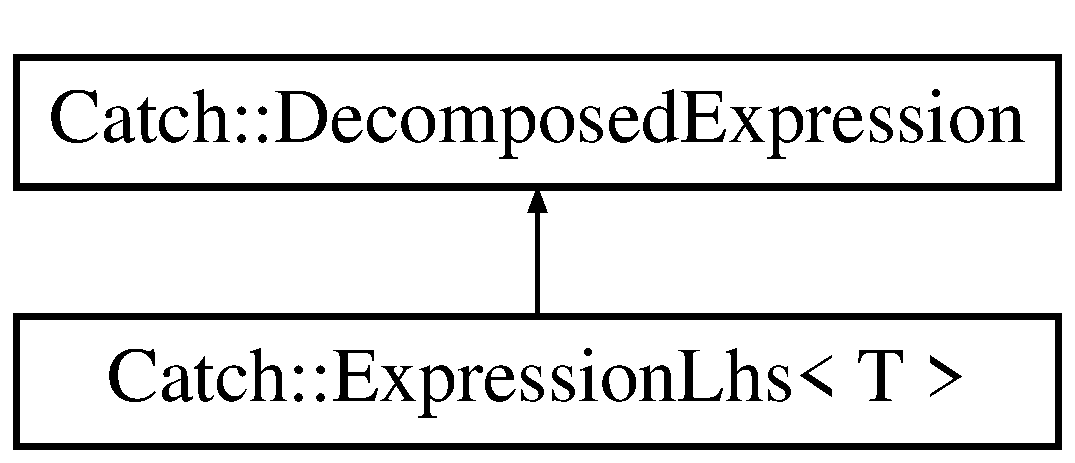
\includegraphics[height=2.000000cm]{class_catch_1_1_expression_lhs}
\end{center}
\end{figure}
\subsection*{Public Member Functions}
\begin{DoxyCompactItemize}
\item 
\mbox{\hyperlink{class_catch_1_1_expression_lhs_aa829588def6146a94fb75de9c4cc482a}{Expression\+Lhs}} (\mbox{\hyperlink{class_catch_1_1_result_builder}{Result\+Builder}} \&rb, T lhs)
\item 
\mbox{\hyperlink{class_catch_1_1_expression_lhs}{Expression\+Lhs}} \& \mbox{\hyperlink{class_catch_1_1_expression_lhs_a60d50fe8adcaabcb7c93747ddbae5993}{operator=}} (const \mbox{\hyperlink{class_catch_1_1_expression_lhs}{Expression\+Lhs}} \&)
\item 
{\footnotesize template$<$typename RhsT $>$ }\\\mbox{\hyperlink{class_catch_1_1_binary_expression}{Binary\+Expression}}$<$ T, \mbox{\hyperlink{namespace_catch_1_1_internal_ae3f96598a7858155750bf38e7295d83ea30e0accba6ec8384f4383b04dd2a6a9e}{Internal\+::\+Is\+Equal\+To}}, RhsT const  \& $>$ \mbox{\hyperlink{class_catch_1_1_expression_lhs_abebe4afc079c91ae548ab8fdba6c77f2}{operator==}} (RhsT const \&rhs)
\item 
{\footnotesize template$<$typename RhsT $>$ }\\\mbox{\hyperlink{class_catch_1_1_binary_expression}{Binary\+Expression}}$<$ T, \mbox{\hyperlink{namespace_catch_1_1_internal_ae3f96598a7858155750bf38e7295d83ea1e1699cf7d3dbee0908f1a123da2456d}{Internal\+::\+Is\+Not\+Equal\+To}}, RhsT const  \& $>$ \mbox{\hyperlink{class_catch_1_1_expression_lhs_a3bc08bb2b9c27678e2628faa73645144}{operator!=}} (RhsT const \&rhs)
\item 
{\footnotesize template$<$typename RhsT $>$ }\\\mbox{\hyperlink{class_catch_1_1_binary_expression}{Binary\+Expression}}$<$ T, \mbox{\hyperlink{namespace_catch_1_1_internal_ae3f96598a7858155750bf38e7295d83eabbbfc41706595e50acbefa8408004b93}{Internal\+::\+Is\+Less\+Than}}, RhsT const  \& $>$ \mbox{\hyperlink{class_catch_1_1_expression_lhs_a919c48e52ff1be5f7329920d4da8e92f}{operator$<$}} (RhsT const \&rhs)
\item 
{\footnotesize template$<$typename RhsT $>$ }\\\mbox{\hyperlink{class_catch_1_1_binary_expression}{Binary\+Expression}}$<$ T, \mbox{\hyperlink{namespace_catch_1_1_internal_ae3f96598a7858155750bf38e7295d83eac0e8866139e99803d169595af70f6c22}{Internal\+::\+Is\+Greater\+Than}}, RhsT const  \& $>$ \mbox{\hyperlink{class_catch_1_1_expression_lhs_a52981d92ec6aad872660ae7df1abb33a}{operator$>$}} (RhsT const \&rhs)
\item 
{\footnotesize template$<$typename RhsT $>$ }\\\mbox{\hyperlink{class_catch_1_1_binary_expression}{Binary\+Expression}}$<$ T, \mbox{\hyperlink{namespace_catch_1_1_internal_ae3f96598a7858155750bf38e7295d83ea0db29a4c3f1e81260036c5e27a8407fd}{Internal\+::\+Is\+Less\+Than\+Or\+Equal\+To}}, RhsT const  \& $>$ \mbox{\hyperlink{class_catch_1_1_expression_lhs_a1d10974a581c67cc400cd6cdd36b0000}{operator$<$=}} (RhsT const \&rhs)
\item 
{\footnotesize template$<$typename RhsT $>$ }\\\mbox{\hyperlink{class_catch_1_1_binary_expression}{Binary\+Expression}}$<$ T, \mbox{\hyperlink{namespace_catch_1_1_internal_ae3f96598a7858155750bf38e7295d83ead2de7e9565e59e36c0987e402203ce1c}{Internal\+::\+Is\+Greater\+Than\+Or\+Equal\+To}}, RhsT const  \& $>$ \mbox{\hyperlink{class_catch_1_1_expression_lhs_a3387a494cb6b699a6c0162c79f7f533c}{operator$>$=}} (RhsT const \&rhs)
\item 
\mbox{\hyperlink{class_catch_1_1_binary_expression}{Binary\+Expression}}$<$ T, \mbox{\hyperlink{namespace_catch_1_1_internal_ae3f96598a7858155750bf38e7295d83ea30e0accba6ec8384f4383b04dd2a6a9e}{Internal\+::\+Is\+Equal\+To}}, bool $>$ \mbox{\hyperlink{class_catch_1_1_expression_lhs_ab803185079504a65b0af95f7c9669351}{operator==}} (bool rhs)
\item 
\mbox{\hyperlink{class_catch_1_1_binary_expression}{Binary\+Expression}}$<$ T, \mbox{\hyperlink{namespace_catch_1_1_internal_ae3f96598a7858155750bf38e7295d83ea1e1699cf7d3dbee0908f1a123da2456d}{Internal\+::\+Is\+Not\+Equal\+To}}, bool $>$ \mbox{\hyperlink{class_catch_1_1_expression_lhs_a1f3ff934880623f12a4cbd9725397ccf}{operator!=}} (bool rhs)
\item 
void \mbox{\hyperlink{class_catch_1_1_expression_lhs_a13d2551a927790284fb5ddf1ee2c9079}{end\+Expression}} ()
\item 
virtual void \mbox{\hyperlink{class_catch_1_1_expression_lhs_a7684a053e8e88a4be475a536252630da}{reconstruct\+Expression}} (std\+::string \&dest) const \mbox{\hyperlink{catch_8hpp_a8ecdce4d3f57835f707915ae831eb847}{C\+A\+T\+C\+H\+\_\+\+O\+V\+E\+R\+R\+I\+DE}}
\end{DoxyCompactItemize}


\subsection{Constructor \& Destructor Documentation}
\mbox{\Hypertarget{class_catch_1_1_expression_lhs_aa829588def6146a94fb75de9c4cc482a}\label{class_catch_1_1_expression_lhs_aa829588def6146a94fb75de9c4cc482a}} 
\index{Catch\+::\+Expression\+Lhs@{Catch\+::\+Expression\+Lhs}!Expression\+Lhs@{Expression\+Lhs}}
\index{Expression\+Lhs@{Expression\+Lhs}!Catch\+::\+Expression\+Lhs@{Catch\+::\+Expression\+Lhs}}
\subsubsection{\texorpdfstring{Expression\+Lhs()}{ExpressionLhs()}}
{\footnotesize\ttfamily template$<$typename T$>$ \\
\mbox{\hyperlink{class_catch_1_1_expression_lhs}{Catch\+::\+Expression\+Lhs}}$<$ T $>$\+::\mbox{\hyperlink{class_catch_1_1_expression_lhs}{Expression\+Lhs}} (\begin{DoxyParamCaption}\item[{\mbox{\hyperlink{class_catch_1_1_result_builder}{Result\+Builder}} \&}]{rb,  }\item[{T}]{lhs }\end{DoxyParamCaption})\hspace{0.3cm}{\ttfamily [inline]}}



\subsection{Member Function Documentation}
\mbox{\Hypertarget{class_catch_1_1_expression_lhs_a13d2551a927790284fb5ddf1ee2c9079}\label{class_catch_1_1_expression_lhs_a13d2551a927790284fb5ddf1ee2c9079}} 
\index{Catch\+::\+Expression\+Lhs@{Catch\+::\+Expression\+Lhs}!end\+Expression@{end\+Expression}}
\index{end\+Expression@{end\+Expression}!Catch\+::\+Expression\+Lhs@{Catch\+::\+Expression\+Lhs}}
\subsubsection{\texorpdfstring{end\+Expression()}{endExpression()}}
{\footnotesize\ttfamily template$<$typename T$>$ \\
void \mbox{\hyperlink{class_catch_1_1_expression_lhs}{Catch\+::\+Expression\+Lhs}}$<$ T $>$\+::end\+Expression (\begin{DoxyParamCaption}{ }\end{DoxyParamCaption})\hspace{0.3cm}{\ttfamily [inline]}}

\mbox{\Hypertarget{class_catch_1_1_expression_lhs_a3bc08bb2b9c27678e2628faa73645144}\label{class_catch_1_1_expression_lhs_a3bc08bb2b9c27678e2628faa73645144}} 
\index{Catch\+::\+Expression\+Lhs@{Catch\+::\+Expression\+Lhs}!operator"!=@{operator"!=}}
\index{operator"!=@{operator"!=}!Catch\+::\+Expression\+Lhs@{Catch\+::\+Expression\+Lhs}}
\subsubsection{\texorpdfstring{operator"!=()}{operator!=()}\hspace{0.1cm}{\footnotesize\ttfamily [1/2]}}
{\footnotesize\ttfamily template$<$typename T$>$ \\
template$<$typename RhsT $>$ \\
\mbox{\hyperlink{class_catch_1_1_binary_expression}{Binary\+Expression}}$<$T, \mbox{\hyperlink{namespace_catch_1_1_internal_ae3f96598a7858155750bf38e7295d83ea1e1699cf7d3dbee0908f1a123da2456d}{Internal\+::\+Is\+Not\+Equal\+To}}, RhsT const\&$>$ \mbox{\hyperlink{class_catch_1_1_expression_lhs}{Catch\+::\+Expression\+Lhs}}$<$ T $>$\+::operator!= (\begin{DoxyParamCaption}\item[{RhsT const \&}]{rhs }\end{DoxyParamCaption})\hspace{0.3cm}{\ttfamily [inline]}}

\mbox{\Hypertarget{class_catch_1_1_expression_lhs_a1f3ff934880623f12a4cbd9725397ccf}\label{class_catch_1_1_expression_lhs_a1f3ff934880623f12a4cbd9725397ccf}} 
\index{Catch\+::\+Expression\+Lhs@{Catch\+::\+Expression\+Lhs}!operator"!=@{operator"!=}}
\index{operator"!=@{operator"!=}!Catch\+::\+Expression\+Lhs@{Catch\+::\+Expression\+Lhs}}
\subsubsection{\texorpdfstring{operator"!=()}{operator!=()}\hspace{0.1cm}{\footnotesize\ttfamily [2/2]}}
{\footnotesize\ttfamily template$<$typename T$>$ \\
\mbox{\hyperlink{class_catch_1_1_binary_expression}{Binary\+Expression}}$<$T, \mbox{\hyperlink{namespace_catch_1_1_internal_ae3f96598a7858155750bf38e7295d83ea1e1699cf7d3dbee0908f1a123da2456d}{Internal\+::\+Is\+Not\+Equal\+To}}, bool$>$ \mbox{\hyperlink{class_catch_1_1_expression_lhs}{Catch\+::\+Expression\+Lhs}}$<$ T $>$\+::operator!= (\begin{DoxyParamCaption}\item[{bool}]{rhs }\end{DoxyParamCaption})\hspace{0.3cm}{\ttfamily [inline]}}

\mbox{\Hypertarget{class_catch_1_1_expression_lhs_a919c48e52ff1be5f7329920d4da8e92f}\label{class_catch_1_1_expression_lhs_a919c48e52ff1be5f7329920d4da8e92f}} 
\index{Catch\+::\+Expression\+Lhs@{Catch\+::\+Expression\+Lhs}!operator$<$@{operator$<$}}
\index{operator$<$@{operator$<$}!Catch\+::\+Expression\+Lhs@{Catch\+::\+Expression\+Lhs}}
\subsubsection{\texorpdfstring{operator$<$()}{operator<()}}
{\footnotesize\ttfamily template$<$typename T$>$ \\
template$<$typename RhsT $>$ \\
\mbox{\hyperlink{class_catch_1_1_binary_expression}{Binary\+Expression}}$<$T, \mbox{\hyperlink{namespace_catch_1_1_internal_ae3f96598a7858155750bf38e7295d83eabbbfc41706595e50acbefa8408004b93}{Internal\+::\+Is\+Less\+Than}}, RhsT const\&$>$ \mbox{\hyperlink{class_catch_1_1_expression_lhs}{Catch\+::\+Expression\+Lhs}}$<$ T $>$\+::operator$<$ (\begin{DoxyParamCaption}\item[{RhsT const \&}]{rhs }\end{DoxyParamCaption})\hspace{0.3cm}{\ttfamily [inline]}}

\mbox{\Hypertarget{class_catch_1_1_expression_lhs_a1d10974a581c67cc400cd6cdd36b0000}\label{class_catch_1_1_expression_lhs_a1d10974a581c67cc400cd6cdd36b0000}} 
\index{Catch\+::\+Expression\+Lhs@{Catch\+::\+Expression\+Lhs}!operator$<$=@{operator$<$=}}
\index{operator$<$=@{operator$<$=}!Catch\+::\+Expression\+Lhs@{Catch\+::\+Expression\+Lhs}}
\subsubsection{\texorpdfstring{operator$<$=()}{operator<=()}}
{\footnotesize\ttfamily template$<$typename T$>$ \\
template$<$typename RhsT $>$ \\
\mbox{\hyperlink{class_catch_1_1_binary_expression}{Binary\+Expression}}$<$T, \mbox{\hyperlink{namespace_catch_1_1_internal_ae3f96598a7858155750bf38e7295d83ea0db29a4c3f1e81260036c5e27a8407fd}{Internal\+::\+Is\+Less\+Than\+Or\+Equal\+To}}, RhsT const\&$>$ \mbox{\hyperlink{class_catch_1_1_expression_lhs}{Catch\+::\+Expression\+Lhs}}$<$ T $>$\+::operator$<$= (\begin{DoxyParamCaption}\item[{RhsT const \&}]{rhs }\end{DoxyParamCaption})\hspace{0.3cm}{\ttfamily [inline]}}

\mbox{\Hypertarget{class_catch_1_1_expression_lhs_a60d50fe8adcaabcb7c93747ddbae5993}\label{class_catch_1_1_expression_lhs_a60d50fe8adcaabcb7c93747ddbae5993}} 
\index{Catch\+::\+Expression\+Lhs@{Catch\+::\+Expression\+Lhs}!operator=@{operator=}}
\index{operator=@{operator=}!Catch\+::\+Expression\+Lhs@{Catch\+::\+Expression\+Lhs}}
\subsubsection{\texorpdfstring{operator=()}{operator=()}}
{\footnotesize\ttfamily template$<$typename T$>$ \\
\mbox{\hyperlink{class_catch_1_1_expression_lhs}{Expression\+Lhs}}\& \mbox{\hyperlink{class_catch_1_1_expression_lhs}{Catch\+::\+Expression\+Lhs}}$<$ T $>$\+::operator= (\begin{DoxyParamCaption}\item[{const \mbox{\hyperlink{class_catch_1_1_expression_lhs}{Expression\+Lhs}}$<$ T $>$ \&}]{ }\end{DoxyParamCaption})}

\mbox{\Hypertarget{class_catch_1_1_expression_lhs_abebe4afc079c91ae548ab8fdba6c77f2}\label{class_catch_1_1_expression_lhs_abebe4afc079c91ae548ab8fdba6c77f2}} 
\index{Catch\+::\+Expression\+Lhs@{Catch\+::\+Expression\+Lhs}!operator==@{operator==}}
\index{operator==@{operator==}!Catch\+::\+Expression\+Lhs@{Catch\+::\+Expression\+Lhs}}
\subsubsection{\texorpdfstring{operator==()}{operator==()}\hspace{0.1cm}{\footnotesize\ttfamily [1/2]}}
{\footnotesize\ttfamily template$<$typename T$>$ \\
template$<$typename RhsT $>$ \\
\mbox{\hyperlink{class_catch_1_1_binary_expression}{Binary\+Expression}}$<$T, \mbox{\hyperlink{namespace_catch_1_1_internal_ae3f96598a7858155750bf38e7295d83ea30e0accba6ec8384f4383b04dd2a6a9e}{Internal\+::\+Is\+Equal\+To}}, RhsT const\&$>$ \mbox{\hyperlink{class_catch_1_1_expression_lhs}{Catch\+::\+Expression\+Lhs}}$<$ T $>$\+::operator== (\begin{DoxyParamCaption}\item[{RhsT const \&}]{rhs }\end{DoxyParamCaption})\hspace{0.3cm}{\ttfamily [inline]}}

\mbox{\Hypertarget{class_catch_1_1_expression_lhs_ab803185079504a65b0af95f7c9669351}\label{class_catch_1_1_expression_lhs_ab803185079504a65b0af95f7c9669351}} 
\index{Catch\+::\+Expression\+Lhs@{Catch\+::\+Expression\+Lhs}!operator==@{operator==}}
\index{operator==@{operator==}!Catch\+::\+Expression\+Lhs@{Catch\+::\+Expression\+Lhs}}
\subsubsection{\texorpdfstring{operator==()}{operator==()}\hspace{0.1cm}{\footnotesize\ttfamily [2/2]}}
{\footnotesize\ttfamily template$<$typename T$>$ \\
\mbox{\hyperlink{class_catch_1_1_binary_expression}{Binary\+Expression}}$<$T, \mbox{\hyperlink{namespace_catch_1_1_internal_ae3f96598a7858155750bf38e7295d83ea30e0accba6ec8384f4383b04dd2a6a9e}{Internal\+::\+Is\+Equal\+To}}, bool$>$ \mbox{\hyperlink{class_catch_1_1_expression_lhs}{Catch\+::\+Expression\+Lhs}}$<$ T $>$\+::operator== (\begin{DoxyParamCaption}\item[{bool}]{rhs }\end{DoxyParamCaption})\hspace{0.3cm}{\ttfamily [inline]}}

\mbox{\Hypertarget{class_catch_1_1_expression_lhs_a52981d92ec6aad872660ae7df1abb33a}\label{class_catch_1_1_expression_lhs_a52981d92ec6aad872660ae7df1abb33a}} 
\index{Catch\+::\+Expression\+Lhs@{Catch\+::\+Expression\+Lhs}!operator$>$@{operator$>$}}
\index{operator$>$@{operator$>$}!Catch\+::\+Expression\+Lhs@{Catch\+::\+Expression\+Lhs}}
\subsubsection{\texorpdfstring{operator$>$()}{operator>()}}
{\footnotesize\ttfamily template$<$typename T$>$ \\
template$<$typename RhsT $>$ \\
\mbox{\hyperlink{class_catch_1_1_binary_expression}{Binary\+Expression}}$<$T, \mbox{\hyperlink{namespace_catch_1_1_internal_ae3f96598a7858155750bf38e7295d83eac0e8866139e99803d169595af70f6c22}{Internal\+::\+Is\+Greater\+Than}}, RhsT const\&$>$ \mbox{\hyperlink{class_catch_1_1_expression_lhs}{Catch\+::\+Expression\+Lhs}}$<$ T $>$\+::operator$>$ (\begin{DoxyParamCaption}\item[{RhsT const \&}]{rhs }\end{DoxyParamCaption})\hspace{0.3cm}{\ttfamily [inline]}}

\mbox{\Hypertarget{class_catch_1_1_expression_lhs_a3387a494cb6b699a6c0162c79f7f533c}\label{class_catch_1_1_expression_lhs_a3387a494cb6b699a6c0162c79f7f533c}} 
\index{Catch\+::\+Expression\+Lhs@{Catch\+::\+Expression\+Lhs}!operator$>$=@{operator$>$=}}
\index{operator$>$=@{operator$>$=}!Catch\+::\+Expression\+Lhs@{Catch\+::\+Expression\+Lhs}}
\subsubsection{\texorpdfstring{operator$>$=()}{operator>=()}}
{\footnotesize\ttfamily template$<$typename T$>$ \\
template$<$typename RhsT $>$ \\
\mbox{\hyperlink{class_catch_1_1_binary_expression}{Binary\+Expression}}$<$T, \mbox{\hyperlink{namespace_catch_1_1_internal_ae3f96598a7858155750bf38e7295d83ead2de7e9565e59e36c0987e402203ce1c}{Internal\+::\+Is\+Greater\+Than\+Or\+Equal\+To}}, RhsT const\&$>$ \mbox{\hyperlink{class_catch_1_1_expression_lhs}{Catch\+::\+Expression\+Lhs}}$<$ T $>$\+::operator$>$= (\begin{DoxyParamCaption}\item[{RhsT const \&}]{rhs }\end{DoxyParamCaption})\hspace{0.3cm}{\ttfamily [inline]}}

\mbox{\Hypertarget{class_catch_1_1_expression_lhs_a7684a053e8e88a4be475a536252630da}\label{class_catch_1_1_expression_lhs_a7684a053e8e88a4be475a536252630da}} 
\index{Catch\+::\+Expression\+Lhs@{Catch\+::\+Expression\+Lhs}!reconstruct\+Expression@{reconstruct\+Expression}}
\index{reconstruct\+Expression@{reconstruct\+Expression}!Catch\+::\+Expression\+Lhs@{Catch\+::\+Expression\+Lhs}}
\subsubsection{\texorpdfstring{reconstruct\+Expression()}{reconstructExpression()}}
{\footnotesize\ttfamily template$<$typename T$>$ \\
virtual void \mbox{\hyperlink{class_catch_1_1_expression_lhs}{Catch\+::\+Expression\+Lhs}}$<$ T $>$\+::reconstruct\+Expression (\begin{DoxyParamCaption}\item[{std\+::string \&}]{dest }\end{DoxyParamCaption}) const\hspace{0.3cm}{\ttfamily [inline]}, {\ttfamily [virtual]}}



Implements \mbox{\hyperlink{struct_catch_1_1_decomposed_expression_a9ce7f356dc96f11f80e40c82f5aa7e55}{Catch\+::\+Decomposed\+Expression}}.



The documentation for this class was generated from the following file\+:\begin{DoxyCompactItemize}
\item 
include/\mbox{\hyperlink{catch_8hpp}{catch.\+hpp}}\end{DoxyCompactItemize}

\hypertarget{struct_catch_1_1_detail_1_1_false_type}{}\section{Catch\+:\+:Detail\+:\+:False\+Type Struct Reference}
\label{struct_catch_1_1_detail_1_1_false_type}\index{Catch\+::\+Detail\+::\+False\+Type@{Catch\+::\+Detail\+::\+False\+Type}}


{\ttfamily \#include $<$catch.\+hpp$>$}

\subsection*{Public Attributes}
\begin{DoxyCompactItemize}
\item 
char \mbox{\hyperlink{struct_catch_1_1_detail_1_1_false_type_abc1a730e197d6f7750ae8aaf47b63477}{sizer}} \mbox{[}2\mbox{]}
\end{DoxyCompactItemize}


\subsection{Member Data Documentation}
\mbox{\Hypertarget{struct_catch_1_1_detail_1_1_false_type_abc1a730e197d6f7750ae8aaf47b63477}\label{struct_catch_1_1_detail_1_1_false_type_abc1a730e197d6f7750ae8aaf47b63477}} 
\index{Catch\+::\+Detail\+::\+False\+Type@{Catch\+::\+Detail\+::\+False\+Type}!sizer@{sizer}}
\index{sizer@{sizer}!Catch\+::\+Detail\+::\+False\+Type@{Catch\+::\+Detail\+::\+False\+Type}}
\subsubsection{\texorpdfstring{sizer}{sizer}}
{\footnotesize\ttfamily char Catch\+::\+Detail\+::\+False\+Type\+::sizer\mbox{[}2\mbox{]}}



The documentation for this struct was generated from the following file\+:\begin{DoxyCompactItemize}
\item 
include/\mbox{\hyperlink{catch_8hpp}{catch.\+hpp}}\end{DoxyCompactItemize}

\hypertarget{struct_catch_1_1_i_context}{}\section{Catch\+:\+:I\+Context Struct Reference}
\label{struct_catch_1_1_i_context}\index{Catch\+::\+I\+Context@{Catch\+::\+I\+Context}}


{\ttfamily \#include $<$catch.\+hpp$>$}

Inheritance diagram for Catch\+:\+:I\+Context\+:\begin{figure}[H]
\begin{center}
\leavevmode
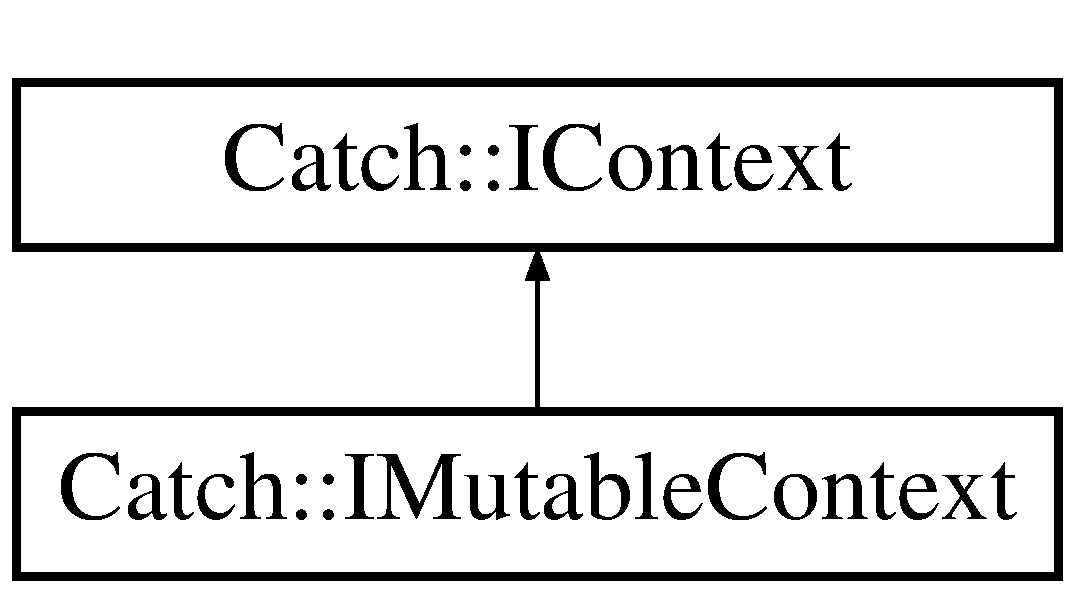
\includegraphics[height=2.000000cm]{struct_catch_1_1_i_context}
\end{center}
\end{figure}
\subsection*{Public Member Functions}
\begin{DoxyCompactItemize}
\item 
virtual \mbox{\hyperlink{struct_catch_1_1_i_context_aeb17355c1be6c2ced5407cad7202628d}{$\sim$\+I\+Context}} ()
\item 
virtual \mbox{\hyperlink{struct_catch_1_1_i_result_capture}{I\+Result\+Capture}} $\ast$ \mbox{\hyperlink{struct_catch_1_1_i_context_a684e4ae71d1fdf3060c352ecde1d122f}{get\+Result\+Capture}} ()=0
\item 
virtual \mbox{\hyperlink{struct_catch_1_1_i_runner}{I\+Runner}} $\ast$ \mbox{\hyperlink{struct_catch_1_1_i_context_af088415dde18d039ed5a2f95b02767c6}{get\+Runner}} ()=0
\item 
virtual size\+\_\+t \mbox{\hyperlink{struct_catch_1_1_i_context_a43e07088db43299ba129fbe6d3106e95}{get\+Generator\+Index}} (std\+::string const \&file\+Info, size\+\_\+t total\+Size)=0
\item 
virtual bool \mbox{\hyperlink{struct_catch_1_1_i_context_a806f7c4ed24d51adae90418e661b24b7}{advance\+Generators\+For\+Current\+Test}} ()=0
\item 
virtual \mbox{\hyperlink{class_catch_1_1_ptr}{Ptr}}$<$ I\+Config const  $>$ \mbox{\hyperlink{struct_catch_1_1_i_context_aee81c415899262e096ad8d6f686fa365}{get\+Config}} () const =0
\end{DoxyCompactItemize}


\subsection{Constructor \& Destructor Documentation}
\mbox{\Hypertarget{struct_catch_1_1_i_context_aeb17355c1be6c2ced5407cad7202628d}\label{struct_catch_1_1_i_context_aeb17355c1be6c2ced5407cad7202628d}} 
\index{Catch\+::\+I\+Context@{Catch\+::\+I\+Context}!````~I\+Context@{$\sim$\+I\+Context}}
\index{````~I\+Context@{$\sim$\+I\+Context}!Catch\+::\+I\+Context@{Catch\+::\+I\+Context}}
\subsubsection{\texorpdfstring{$\sim$\+I\+Context()}{~IContext()}}
{\footnotesize\ttfamily virtual Catch\+::\+I\+Context\+::$\sim$\+I\+Context (\begin{DoxyParamCaption}{ }\end{DoxyParamCaption})\hspace{0.3cm}{\ttfamily [virtual]}}



\subsection{Member Function Documentation}
\mbox{\Hypertarget{struct_catch_1_1_i_context_a806f7c4ed24d51adae90418e661b24b7}\label{struct_catch_1_1_i_context_a806f7c4ed24d51adae90418e661b24b7}} 
\index{Catch\+::\+I\+Context@{Catch\+::\+I\+Context}!advance\+Generators\+For\+Current\+Test@{advance\+Generators\+For\+Current\+Test}}
\index{advance\+Generators\+For\+Current\+Test@{advance\+Generators\+For\+Current\+Test}!Catch\+::\+I\+Context@{Catch\+::\+I\+Context}}
\subsubsection{\texorpdfstring{advance\+Generators\+For\+Current\+Test()}{advanceGeneratorsForCurrentTest()}}
{\footnotesize\ttfamily virtual bool Catch\+::\+I\+Context\+::advance\+Generators\+For\+Current\+Test (\begin{DoxyParamCaption}{ }\end{DoxyParamCaption})\hspace{0.3cm}{\ttfamily [pure virtual]}}

\mbox{\Hypertarget{struct_catch_1_1_i_context_aee81c415899262e096ad8d6f686fa365}\label{struct_catch_1_1_i_context_aee81c415899262e096ad8d6f686fa365}} 
\index{Catch\+::\+I\+Context@{Catch\+::\+I\+Context}!get\+Config@{get\+Config}}
\index{get\+Config@{get\+Config}!Catch\+::\+I\+Context@{Catch\+::\+I\+Context}}
\subsubsection{\texorpdfstring{get\+Config()}{getConfig()}}
{\footnotesize\ttfamily virtual \mbox{\hyperlink{class_catch_1_1_ptr}{Ptr}}$<$I\+Config const$>$ Catch\+::\+I\+Context\+::get\+Config (\begin{DoxyParamCaption}{ }\end{DoxyParamCaption}) const\hspace{0.3cm}{\ttfamily [pure virtual]}}

\mbox{\Hypertarget{struct_catch_1_1_i_context_a43e07088db43299ba129fbe6d3106e95}\label{struct_catch_1_1_i_context_a43e07088db43299ba129fbe6d3106e95}} 
\index{Catch\+::\+I\+Context@{Catch\+::\+I\+Context}!get\+Generator\+Index@{get\+Generator\+Index}}
\index{get\+Generator\+Index@{get\+Generator\+Index}!Catch\+::\+I\+Context@{Catch\+::\+I\+Context}}
\subsubsection{\texorpdfstring{get\+Generator\+Index()}{getGeneratorIndex()}}
{\footnotesize\ttfamily virtual size\+\_\+t Catch\+::\+I\+Context\+::get\+Generator\+Index (\begin{DoxyParamCaption}\item[{std\+::string const \&}]{file\+Info,  }\item[{size\+\_\+t}]{total\+Size }\end{DoxyParamCaption})\hspace{0.3cm}{\ttfamily [pure virtual]}}

\mbox{\Hypertarget{struct_catch_1_1_i_context_a684e4ae71d1fdf3060c352ecde1d122f}\label{struct_catch_1_1_i_context_a684e4ae71d1fdf3060c352ecde1d122f}} 
\index{Catch\+::\+I\+Context@{Catch\+::\+I\+Context}!get\+Result\+Capture@{get\+Result\+Capture}}
\index{get\+Result\+Capture@{get\+Result\+Capture}!Catch\+::\+I\+Context@{Catch\+::\+I\+Context}}
\subsubsection{\texorpdfstring{get\+Result\+Capture()}{getResultCapture()}}
{\footnotesize\ttfamily virtual \mbox{\hyperlink{struct_catch_1_1_i_result_capture}{I\+Result\+Capture}}$\ast$ Catch\+::\+I\+Context\+::get\+Result\+Capture (\begin{DoxyParamCaption}{ }\end{DoxyParamCaption})\hspace{0.3cm}{\ttfamily [pure virtual]}}

\mbox{\Hypertarget{struct_catch_1_1_i_context_af088415dde18d039ed5a2f95b02767c6}\label{struct_catch_1_1_i_context_af088415dde18d039ed5a2f95b02767c6}} 
\index{Catch\+::\+I\+Context@{Catch\+::\+I\+Context}!get\+Runner@{get\+Runner}}
\index{get\+Runner@{get\+Runner}!Catch\+::\+I\+Context@{Catch\+::\+I\+Context}}
\subsubsection{\texorpdfstring{get\+Runner()}{getRunner()}}
{\footnotesize\ttfamily virtual \mbox{\hyperlink{struct_catch_1_1_i_runner}{I\+Runner}}$\ast$ Catch\+::\+I\+Context\+::get\+Runner (\begin{DoxyParamCaption}{ }\end{DoxyParamCaption})\hspace{0.3cm}{\ttfamily [pure virtual]}}



The documentation for this struct was generated from the following file\+:\begin{DoxyCompactItemize}
\item 
include/\mbox{\hyperlink{catch_8hpp}{catch.\+hpp}}\end{DoxyCompactItemize}

\hypertarget{struct_catch_1_1_i_exception_translator}{}\section{Catch\+:\+:I\+Exception\+Translator Struct Reference}
\label{struct_catch_1_1_i_exception_translator}\index{Catch\+::\+I\+Exception\+Translator@{Catch\+::\+I\+Exception\+Translator}}


{\ttfamily \#include $<$catch.\+hpp$>$}

\subsection*{Public Member Functions}
\begin{DoxyCompactItemize}
\item 
virtual \mbox{\hyperlink{struct_catch_1_1_i_exception_translator_afa00bb6258c07591df472aadae05783f}{$\sim$\+I\+Exception\+Translator}} ()
\item 
virtual std\+::string \mbox{\hyperlink{struct_catch_1_1_i_exception_translator_a2a554b96ed5ed411e7c796b6b42837a5}{translate}} (Exception\+Translators\+::const\+\_\+iterator it, Exception\+Translators\+::const\+\_\+iterator it\+End) const =0
\end{DoxyCompactItemize}


\subsection{Constructor \& Destructor Documentation}
\mbox{\Hypertarget{struct_catch_1_1_i_exception_translator_afa00bb6258c07591df472aadae05783f}\label{struct_catch_1_1_i_exception_translator_afa00bb6258c07591df472aadae05783f}} 
\index{Catch\+::\+I\+Exception\+Translator@{Catch\+::\+I\+Exception\+Translator}!````~I\+Exception\+Translator@{$\sim$\+I\+Exception\+Translator}}
\index{````~I\+Exception\+Translator@{$\sim$\+I\+Exception\+Translator}!Catch\+::\+I\+Exception\+Translator@{Catch\+::\+I\+Exception\+Translator}}
\subsubsection{\texorpdfstring{$\sim$\+I\+Exception\+Translator()}{~IExceptionTranslator()}}
{\footnotesize\ttfamily virtual Catch\+::\+I\+Exception\+Translator\+::$\sim$\+I\+Exception\+Translator (\begin{DoxyParamCaption}{ }\end{DoxyParamCaption})\hspace{0.3cm}{\ttfamily [virtual]}}



\subsection{Member Function Documentation}
\mbox{\Hypertarget{struct_catch_1_1_i_exception_translator_a2a554b96ed5ed411e7c796b6b42837a5}\label{struct_catch_1_1_i_exception_translator_a2a554b96ed5ed411e7c796b6b42837a5}} 
\index{Catch\+::\+I\+Exception\+Translator@{Catch\+::\+I\+Exception\+Translator}!translate@{translate}}
\index{translate@{translate}!Catch\+::\+I\+Exception\+Translator@{Catch\+::\+I\+Exception\+Translator}}
\subsubsection{\texorpdfstring{translate()}{translate()}}
{\footnotesize\ttfamily virtual std\+::string Catch\+::\+I\+Exception\+Translator\+::translate (\begin{DoxyParamCaption}\item[{Exception\+Translators\+::const\+\_\+iterator}]{it,  }\item[{Exception\+Translators\+::const\+\_\+iterator}]{it\+End }\end{DoxyParamCaption}) const\hspace{0.3cm}{\ttfamily [pure virtual]}}



The documentation for this struct was generated from the following file\+:\begin{DoxyCompactItemize}
\item 
include/\mbox{\hyperlink{catch_8hpp}{catch.\+hpp}}\end{DoxyCompactItemize}

\hypertarget{struct_catch_1_1_i_exception_translator_registry}{}\section{Catch\+:\+:I\+Exception\+Translator\+Registry Struct Reference}
\label{struct_catch_1_1_i_exception_translator_registry}\index{Catch\+::\+I\+Exception\+Translator\+Registry@{Catch\+::\+I\+Exception\+Translator\+Registry}}


{\ttfamily \#include $<$catch.\+hpp$>$}

\subsection*{Public Member Functions}
\begin{DoxyCompactItemize}
\item 
virtual \mbox{\hyperlink{struct_catch_1_1_i_exception_translator_registry_acf7402e18789ea46d54ea8564ac358d3}{$\sim$\+I\+Exception\+Translator\+Registry}} ()
\item 
virtual std\+::string \mbox{\hyperlink{struct_catch_1_1_i_exception_translator_registry_af76ae8c331a17f2a94c9720bc0d686bb}{translate\+Active\+Exception}} () const =0
\end{DoxyCompactItemize}


\subsection{Constructor \& Destructor Documentation}
\mbox{\Hypertarget{struct_catch_1_1_i_exception_translator_registry_acf7402e18789ea46d54ea8564ac358d3}\label{struct_catch_1_1_i_exception_translator_registry_acf7402e18789ea46d54ea8564ac358d3}} 
\index{Catch\+::\+I\+Exception\+Translator\+Registry@{Catch\+::\+I\+Exception\+Translator\+Registry}!````~I\+Exception\+Translator\+Registry@{$\sim$\+I\+Exception\+Translator\+Registry}}
\index{````~I\+Exception\+Translator\+Registry@{$\sim$\+I\+Exception\+Translator\+Registry}!Catch\+::\+I\+Exception\+Translator\+Registry@{Catch\+::\+I\+Exception\+Translator\+Registry}}
\subsubsection{\texorpdfstring{$\sim$\+I\+Exception\+Translator\+Registry()}{~IExceptionTranslatorRegistry()}}
{\footnotesize\ttfamily virtual Catch\+::\+I\+Exception\+Translator\+Registry\+::$\sim$\+I\+Exception\+Translator\+Registry (\begin{DoxyParamCaption}{ }\end{DoxyParamCaption})\hspace{0.3cm}{\ttfamily [virtual]}}



\subsection{Member Function Documentation}
\mbox{\Hypertarget{struct_catch_1_1_i_exception_translator_registry_af76ae8c331a17f2a94c9720bc0d686bb}\label{struct_catch_1_1_i_exception_translator_registry_af76ae8c331a17f2a94c9720bc0d686bb}} 
\index{Catch\+::\+I\+Exception\+Translator\+Registry@{Catch\+::\+I\+Exception\+Translator\+Registry}!translate\+Active\+Exception@{translate\+Active\+Exception}}
\index{translate\+Active\+Exception@{translate\+Active\+Exception}!Catch\+::\+I\+Exception\+Translator\+Registry@{Catch\+::\+I\+Exception\+Translator\+Registry}}
\subsubsection{\texorpdfstring{translate\+Active\+Exception()}{translateActiveException()}}
{\footnotesize\ttfamily virtual std\+::string Catch\+::\+I\+Exception\+Translator\+Registry\+::translate\+Active\+Exception (\begin{DoxyParamCaption}{ }\end{DoxyParamCaption}) const\hspace{0.3cm}{\ttfamily [pure virtual]}}



The documentation for this struct was generated from the following file\+:\begin{DoxyCompactItemize}
\item 
include/\mbox{\hyperlink{catch_8hpp}{catch.\+hpp}}\end{DoxyCompactItemize}

\hypertarget{struct_catch_1_1_i_generator}{}\section{Catch\+:\+:I\+Generator$<$ T $>$ Struct Template Reference}
\label{struct_catch_1_1_i_generator}\index{Catch\+::\+I\+Generator$<$ T $>$@{Catch\+::\+I\+Generator$<$ T $>$}}


{\ttfamily \#include $<$catch.\+hpp$>$}

Inheritance diagram for Catch\+:\+:I\+Generator$<$ T $>$\+:\begin{figure}[H]
\begin{center}
\leavevmode
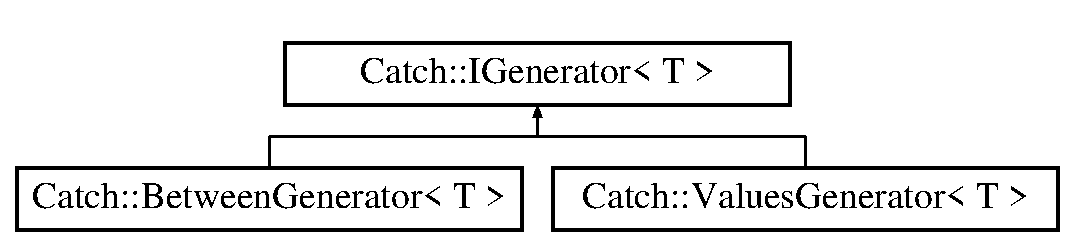
\includegraphics[height=2.000000cm]{struct_catch_1_1_i_generator}
\end{center}
\end{figure}
\subsection*{Public Member Functions}
\begin{DoxyCompactItemize}
\item 
virtual \mbox{\hyperlink{struct_catch_1_1_i_generator_a0622037f4617e09aa8c584b0144d4a1a}{$\sim$\+I\+Generator}} ()
\item 
virtual T \mbox{\hyperlink{struct_catch_1_1_i_generator_ad69e937cb66dba3ed9429c42abf4fce3}{get\+Value}} (std\+::size\+\_\+t index) const =0
\item 
virtual std\+::size\+\_\+t \mbox{\hyperlink{struct_catch_1_1_i_generator_a2e317253b03e838b6065ce69719a198e}{size}} () const =0
\end{DoxyCompactItemize}


\subsection{Constructor \& Destructor Documentation}
\mbox{\Hypertarget{struct_catch_1_1_i_generator_a0622037f4617e09aa8c584b0144d4a1a}\label{struct_catch_1_1_i_generator_a0622037f4617e09aa8c584b0144d4a1a}} 
\index{Catch\+::\+I\+Generator@{Catch\+::\+I\+Generator}!````~I\+Generator@{$\sim$\+I\+Generator}}
\index{````~I\+Generator@{$\sim$\+I\+Generator}!Catch\+::\+I\+Generator@{Catch\+::\+I\+Generator}}
\subsubsection{\texorpdfstring{$\sim$\+I\+Generator()}{~IGenerator()}}
{\footnotesize\ttfamily template$<$typename T$>$ \\
virtual \mbox{\hyperlink{struct_catch_1_1_i_generator}{Catch\+::\+I\+Generator}}$<$ T $>$\+::$\sim$\mbox{\hyperlink{struct_catch_1_1_i_generator}{I\+Generator}} (\begin{DoxyParamCaption}{ }\end{DoxyParamCaption})\hspace{0.3cm}{\ttfamily [inline]}, {\ttfamily [virtual]}}



\subsection{Member Function Documentation}
\mbox{\Hypertarget{struct_catch_1_1_i_generator_ad69e937cb66dba3ed9429c42abf4fce3}\label{struct_catch_1_1_i_generator_ad69e937cb66dba3ed9429c42abf4fce3}} 
\index{Catch\+::\+I\+Generator@{Catch\+::\+I\+Generator}!get\+Value@{get\+Value}}
\index{get\+Value@{get\+Value}!Catch\+::\+I\+Generator@{Catch\+::\+I\+Generator}}
\subsubsection{\texorpdfstring{get\+Value()}{getValue()}}
{\footnotesize\ttfamily template$<$typename T$>$ \\
virtual T \mbox{\hyperlink{struct_catch_1_1_i_generator}{Catch\+::\+I\+Generator}}$<$ T $>$\+::get\+Value (\begin{DoxyParamCaption}\item[{std\+::size\+\_\+t}]{index }\end{DoxyParamCaption}) const\hspace{0.3cm}{\ttfamily [pure virtual]}}



Implemented in \mbox{\hyperlink{class_catch_1_1_values_generator_a9674c8b70d562d2d68154de92dd1810a}{Catch\+::\+Values\+Generator$<$ T $>$}}, and \mbox{\hyperlink{class_catch_1_1_between_generator_a913f74bb0c23b3bc0127abfffdabbd94}{Catch\+::\+Between\+Generator$<$ T $>$}}.

\mbox{\Hypertarget{struct_catch_1_1_i_generator_a2e317253b03e838b6065ce69719a198e}\label{struct_catch_1_1_i_generator_a2e317253b03e838b6065ce69719a198e}} 
\index{Catch\+::\+I\+Generator@{Catch\+::\+I\+Generator}!size@{size}}
\index{size@{size}!Catch\+::\+I\+Generator@{Catch\+::\+I\+Generator}}
\subsubsection{\texorpdfstring{size()}{size()}}
{\footnotesize\ttfamily template$<$typename T$>$ \\
virtual std\+::size\+\_\+t \mbox{\hyperlink{struct_catch_1_1_i_generator}{Catch\+::\+I\+Generator}}$<$ T $>$\+::size (\begin{DoxyParamCaption}{ }\end{DoxyParamCaption}) const\hspace{0.3cm}{\ttfamily [pure virtual]}}



Implemented in \mbox{\hyperlink{class_catch_1_1_values_generator_a9aa5b140ee502975cf35115e534ab771}{Catch\+::\+Values\+Generator$<$ T $>$}}, and \mbox{\hyperlink{class_catch_1_1_between_generator_af65a1fe51f9b1106fc676e3dd189adb6}{Catch\+::\+Between\+Generator$<$ T $>$}}.



The documentation for this struct was generated from the following file\+:\begin{DoxyCompactItemize}
\item 
include/\mbox{\hyperlink{catch_8hpp}{catch.\+hpp}}\end{DoxyCompactItemize}

\hypertarget{struct_catch_1_1_i_generator_info}{}\section{Catch\+:\+:I\+Generator\+Info Struct Reference}
\label{struct_catch_1_1_i_generator_info}\index{Catch\+::\+I\+Generator\+Info@{Catch\+::\+I\+Generator\+Info}}


{\ttfamily \#include $<$catch.\+hpp$>$}

\subsection*{Public Member Functions}
\begin{DoxyCompactItemize}
\item 
virtual \mbox{\hyperlink{struct_catch_1_1_i_generator_info_a9266aa62993298510c2a8b5948abb8e6}{$\sim$\+I\+Generator\+Info}} ()
\item 
virtual bool \mbox{\hyperlink{struct_catch_1_1_i_generator_info_a2b86711ca7009903edfe27ed62b515ef}{move\+Next}} ()=0
\item 
virtual std\+::size\+\_\+t \mbox{\hyperlink{struct_catch_1_1_i_generator_info_a6a0dca712d31f6849fd9447b1344673a}{get\+Current\+Index}} () const =0
\end{DoxyCompactItemize}


\subsection{Constructor \& Destructor Documentation}
\mbox{\Hypertarget{struct_catch_1_1_i_generator_info_a9266aa62993298510c2a8b5948abb8e6}\label{struct_catch_1_1_i_generator_info_a9266aa62993298510c2a8b5948abb8e6}} 
\index{Catch\+::\+I\+Generator\+Info@{Catch\+::\+I\+Generator\+Info}!````~I\+Generator\+Info@{$\sim$\+I\+Generator\+Info}}
\index{````~I\+Generator\+Info@{$\sim$\+I\+Generator\+Info}!Catch\+::\+I\+Generator\+Info@{Catch\+::\+I\+Generator\+Info}}
\subsubsection{\texorpdfstring{$\sim$\+I\+Generator\+Info()}{~IGeneratorInfo()}}
{\footnotesize\ttfamily virtual Catch\+::\+I\+Generator\+Info\+::$\sim$\+I\+Generator\+Info (\begin{DoxyParamCaption}{ }\end{DoxyParamCaption})\hspace{0.3cm}{\ttfamily [virtual]}}



\subsection{Member Function Documentation}
\mbox{\Hypertarget{struct_catch_1_1_i_generator_info_a6a0dca712d31f6849fd9447b1344673a}\label{struct_catch_1_1_i_generator_info_a6a0dca712d31f6849fd9447b1344673a}} 
\index{Catch\+::\+I\+Generator\+Info@{Catch\+::\+I\+Generator\+Info}!get\+Current\+Index@{get\+Current\+Index}}
\index{get\+Current\+Index@{get\+Current\+Index}!Catch\+::\+I\+Generator\+Info@{Catch\+::\+I\+Generator\+Info}}
\subsubsection{\texorpdfstring{get\+Current\+Index()}{getCurrentIndex()}}
{\footnotesize\ttfamily virtual std\+::size\+\_\+t Catch\+::\+I\+Generator\+Info\+::get\+Current\+Index (\begin{DoxyParamCaption}{ }\end{DoxyParamCaption}) const\hspace{0.3cm}{\ttfamily [pure virtual]}}

\mbox{\Hypertarget{struct_catch_1_1_i_generator_info_a2b86711ca7009903edfe27ed62b515ef}\label{struct_catch_1_1_i_generator_info_a2b86711ca7009903edfe27ed62b515ef}} 
\index{Catch\+::\+I\+Generator\+Info@{Catch\+::\+I\+Generator\+Info}!move\+Next@{move\+Next}}
\index{move\+Next@{move\+Next}!Catch\+::\+I\+Generator\+Info@{Catch\+::\+I\+Generator\+Info}}
\subsubsection{\texorpdfstring{move\+Next()}{moveNext()}}
{\footnotesize\ttfamily virtual bool Catch\+::\+I\+Generator\+Info\+::move\+Next (\begin{DoxyParamCaption}{ }\end{DoxyParamCaption})\hspace{0.3cm}{\ttfamily [pure virtual]}}



The documentation for this struct was generated from the following file\+:\begin{DoxyCompactItemize}
\item 
include/\mbox{\hyperlink{catch_8hpp}{catch.\+hpp}}\end{DoxyCompactItemize}

\hypertarget{struct_catch_1_1_i_generators_for_test}{}\section{Catch\+:\+:I\+Generators\+For\+Test Struct Reference}
\label{struct_catch_1_1_i_generators_for_test}\index{Catch\+::\+I\+Generators\+For\+Test@{Catch\+::\+I\+Generators\+For\+Test}}


{\ttfamily \#include $<$catch.\+hpp$>$}

\subsection*{Public Member Functions}
\begin{DoxyCompactItemize}
\item 
virtual \mbox{\hyperlink{struct_catch_1_1_i_generators_for_test_a05725e76ee92e498f73479a61f3e3c7c}{$\sim$\+I\+Generators\+For\+Test}} ()
\item 
virtual \mbox{\hyperlink{struct_catch_1_1_i_generator_info}{I\+Generator\+Info}} \& \mbox{\hyperlink{struct_catch_1_1_i_generators_for_test_a180d84e858840188e4c3788e47eefdb0}{get\+Generator\+Info}} (std\+::string const \&file\+Info, std\+::size\+\_\+t size)=0
\item 
virtual bool \mbox{\hyperlink{struct_catch_1_1_i_generators_for_test_adab31832d529fc584fd63164e0a1c8ad}{move\+Next}} ()=0
\end{DoxyCompactItemize}


\subsection{Constructor \& Destructor Documentation}
\mbox{\Hypertarget{struct_catch_1_1_i_generators_for_test_a05725e76ee92e498f73479a61f3e3c7c}\label{struct_catch_1_1_i_generators_for_test_a05725e76ee92e498f73479a61f3e3c7c}} 
\index{Catch\+::\+I\+Generators\+For\+Test@{Catch\+::\+I\+Generators\+For\+Test}!````~I\+Generators\+For\+Test@{$\sim$\+I\+Generators\+For\+Test}}
\index{````~I\+Generators\+For\+Test@{$\sim$\+I\+Generators\+For\+Test}!Catch\+::\+I\+Generators\+For\+Test@{Catch\+::\+I\+Generators\+For\+Test}}
\subsubsection{\texorpdfstring{$\sim$\+I\+Generators\+For\+Test()}{~IGeneratorsForTest()}}
{\footnotesize\ttfamily virtual Catch\+::\+I\+Generators\+For\+Test\+::$\sim$\+I\+Generators\+For\+Test (\begin{DoxyParamCaption}{ }\end{DoxyParamCaption})\hspace{0.3cm}{\ttfamily [virtual]}}



\subsection{Member Function Documentation}
\mbox{\Hypertarget{struct_catch_1_1_i_generators_for_test_a180d84e858840188e4c3788e47eefdb0}\label{struct_catch_1_1_i_generators_for_test_a180d84e858840188e4c3788e47eefdb0}} 
\index{Catch\+::\+I\+Generators\+For\+Test@{Catch\+::\+I\+Generators\+For\+Test}!get\+Generator\+Info@{get\+Generator\+Info}}
\index{get\+Generator\+Info@{get\+Generator\+Info}!Catch\+::\+I\+Generators\+For\+Test@{Catch\+::\+I\+Generators\+For\+Test}}
\subsubsection{\texorpdfstring{get\+Generator\+Info()}{getGeneratorInfo()}}
{\footnotesize\ttfamily virtual \mbox{\hyperlink{struct_catch_1_1_i_generator_info}{I\+Generator\+Info}}\& Catch\+::\+I\+Generators\+For\+Test\+::get\+Generator\+Info (\begin{DoxyParamCaption}\item[{std\+::string const \&}]{file\+Info,  }\item[{std\+::size\+\_\+t}]{size }\end{DoxyParamCaption})\hspace{0.3cm}{\ttfamily [pure virtual]}}

\mbox{\Hypertarget{struct_catch_1_1_i_generators_for_test_adab31832d529fc584fd63164e0a1c8ad}\label{struct_catch_1_1_i_generators_for_test_adab31832d529fc584fd63164e0a1c8ad}} 
\index{Catch\+::\+I\+Generators\+For\+Test@{Catch\+::\+I\+Generators\+For\+Test}!move\+Next@{move\+Next}}
\index{move\+Next@{move\+Next}!Catch\+::\+I\+Generators\+For\+Test@{Catch\+::\+I\+Generators\+For\+Test}}
\subsubsection{\texorpdfstring{move\+Next()}{moveNext()}}
{\footnotesize\ttfamily virtual bool Catch\+::\+I\+Generators\+For\+Test\+::move\+Next (\begin{DoxyParamCaption}{ }\end{DoxyParamCaption})\hspace{0.3cm}{\ttfamily [pure virtual]}}



The documentation for this struct was generated from the following file\+:\begin{DoxyCompactItemize}
\item 
include/\mbox{\hyperlink{catch_8hpp}{catch.\+hpp}}\end{DoxyCompactItemize}

\hypertarget{struct_catch_1_1_i_mutable_context}{}\section{Catch\+:\+:I\+Mutable\+Context Struct Reference}
\label{struct_catch_1_1_i_mutable_context}\index{Catch\+::\+I\+Mutable\+Context@{Catch\+::\+I\+Mutable\+Context}}


{\ttfamily \#include $<$catch.\+hpp$>$}

Inheritance diagram for Catch\+:\+:I\+Mutable\+Context\+:\begin{figure}[H]
\begin{center}
\leavevmode
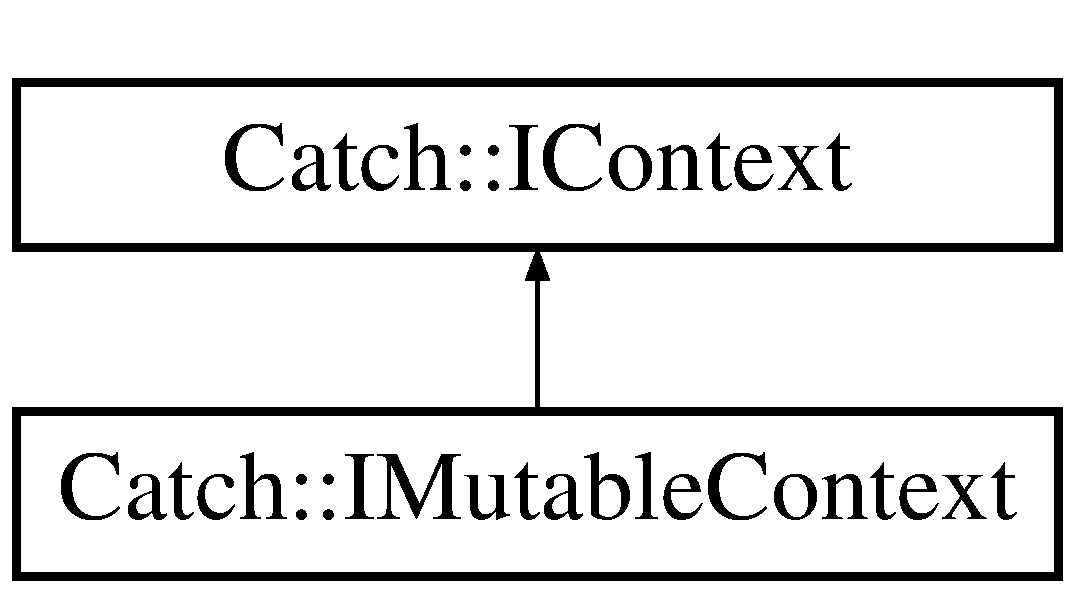
\includegraphics[height=2.000000cm]{struct_catch_1_1_i_mutable_context}
\end{center}
\end{figure}
\subsection*{Public Member Functions}
\begin{DoxyCompactItemize}
\item 
virtual \mbox{\hyperlink{struct_catch_1_1_i_mutable_context_a93f32b2ab6d0fb83637059240be799ab}{$\sim$\+I\+Mutable\+Context}} ()
\item 
virtual void \mbox{\hyperlink{struct_catch_1_1_i_mutable_context_a4a80afd0525b7def21bee8d9b48f2d39}{set\+Result\+Capture}} (\mbox{\hyperlink{struct_catch_1_1_i_result_capture}{I\+Result\+Capture}} $\ast$result\+Capture)=0
\item 
virtual void \mbox{\hyperlink{struct_catch_1_1_i_mutable_context_af2e53b1dea4527a2587cff266a730f6e}{set\+Runner}} (\mbox{\hyperlink{struct_catch_1_1_i_runner}{I\+Runner}} $\ast$runner)=0
\item 
virtual void \mbox{\hyperlink{struct_catch_1_1_i_mutable_context_a013e8f688a8ea7970262d07ead542a63}{set\+Config}} (\mbox{\hyperlink{class_catch_1_1_ptr}{Ptr}}$<$ I\+Config const $>$ const \&config)=0
\end{DoxyCompactItemize}


\subsection{Constructor \& Destructor Documentation}
\mbox{\Hypertarget{struct_catch_1_1_i_mutable_context_a93f32b2ab6d0fb83637059240be799ab}\label{struct_catch_1_1_i_mutable_context_a93f32b2ab6d0fb83637059240be799ab}} 
\index{Catch\+::\+I\+Mutable\+Context@{Catch\+::\+I\+Mutable\+Context}!````~I\+Mutable\+Context@{$\sim$\+I\+Mutable\+Context}}
\index{````~I\+Mutable\+Context@{$\sim$\+I\+Mutable\+Context}!Catch\+::\+I\+Mutable\+Context@{Catch\+::\+I\+Mutable\+Context}}
\subsubsection{\texorpdfstring{$\sim$\+I\+Mutable\+Context()}{~IMutableContext()}}
{\footnotesize\ttfamily virtual Catch\+::\+I\+Mutable\+Context\+::$\sim$\+I\+Mutable\+Context (\begin{DoxyParamCaption}{ }\end{DoxyParamCaption})\hspace{0.3cm}{\ttfamily [virtual]}}



\subsection{Member Function Documentation}
\mbox{\Hypertarget{struct_catch_1_1_i_mutable_context_a013e8f688a8ea7970262d07ead542a63}\label{struct_catch_1_1_i_mutable_context_a013e8f688a8ea7970262d07ead542a63}} 
\index{Catch\+::\+I\+Mutable\+Context@{Catch\+::\+I\+Mutable\+Context}!set\+Config@{set\+Config}}
\index{set\+Config@{set\+Config}!Catch\+::\+I\+Mutable\+Context@{Catch\+::\+I\+Mutable\+Context}}
\subsubsection{\texorpdfstring{set\+Config()}{setConfig()}}
{\footnotesize\ttfamily virtual void Catch\+::\+I\+Mutable\+Context\+::set\+Config (\begin{DoxyParamCaption}\item[{\mbox{\hyperlink{class_catch_1_1_ptr}{Ptr}}$<$ I\+Config const $>$ const \&}]{config }\end{DoxyParamCaption})\hspace{0.3cm}{\ttfamily [pure virtual]}}

\mbox{\Hypertarget{struct_catch_1_1_i_mutable_context_a4a80afd0525b7def21bee8d9b48f2d39}\label{struct_catch_1_1_i_mutable_context_a4a80afd0525b7def21bee8d9b48f2d39}} 
\index{Catch\+::\+I\+Mutable\+Context@{Catch\+::\+I\+Mutable\+Context}!set\+Result\+Capture@{set\+Result\+Capture}}
\index{set\+Result\+Capture@{set\+Result\+Capture}!Catch\+::\+I\+Mutable\+Context@{Catch\+::\+I\+Mutable\+Context}}
\subsubsection{\texorpdfstring{set\+Result\+Capture()}{setResultCapture()}}
{\footnotesize\ttfamily virtual void Catch\+::\+I\+Mutable\+Context\+::set\+Result\+Capture (\begin{DoxyParamCaption}\item[{\mbox{\hyperlink{struct_catch_1_1_i_result_capture}{I\+Result\+Capture}} $\ast$}]{result\+Capture }\end{DoxyParamCaption})\hspace{0.3cm}{\ttfamily [pure virtual]}}

\mbox{\Hypertarget{struct_catch_1_1_i_mutable_context_af2e53b1dea4527a2587cff266a730f6e}\label{struct_catch_1_1_i_mutable_context_af2e53b1dea4527a2587cff266a730f6e}} 
\index{Catch\+::\+I\+Mutable\+Context@{Catch\+::\+I\+Mutable\+Context}!set\+Runner@{set\+Runner}}
\index{set\+Runner@{set\+Runner}!Catch\+::\+I\+Mutable\+Context@{Catch\+::\+I\+Mutable\+Context}}
\subsubsection{\texorpdfstring{set\+Runner()}{setRunner()}}
{\footnotesize\ttfamily virtual void Catch\+::\+I\+Mutable\+Context\+::set\+Runner (\begin{DoxyParamCaption}\item[{\mbox{\hyperlink{struct_catch_1_1_i_runner}{I\+Runner}} $\ast$}]{runner }\end{DoxyParamCaption})\hspace{0.3cm}{\ttfamily [pure virtual]}}



The documentation for this struct was generated from the following file\+:\begin{DoxyCompactItemize}
\item 
include/\mbox{\hyperlink{catch_8hpp}{catch.\+hpp}}\end{DoxyCompactItemize}

\hypertarget{struct_catch_1_1_i_mutable_registry_hub}{}\section{Catch\+:\+:I\+Mutable\+Registry\+Hub Struct Reference}
\label{struct_catch_1_1_i_mutable_registry_hub}\index{Catch\+::\+I\+Mutable\+Registry\+Hub@{Catch\+::\+I\+Mutable\+Registry\+Hub}}


{\ttfamily \#include $<$catch.\+hpp$>$}

\subsection*{Public Member Functions}
\begin{DoxyCompactItemize}
\item 
virtual \mbox{\hyperlink{struct_catch_1_1_i_mutable_registry_hub_a759ca1e044e19f905fb4d306f1367193}{$\sim$\+I\+Mutable\+Registry\+Hub}} ()
\item 
virtual void \mbox{\hyperlink{struct_catch_1_1_i_mutable_registry_hub_aab72d0aa1fa14627f1a6a4c893ae0a12}{register\+Reporter}} (std\+::string const \&name, \mbox{\hyperlink{class_catch_1_1_ptr}{Ptr}}$<$ I\+Reporter\+Factory $>$ const \&factory)=0
\item 
virtual void \mbox{\hyperlink{struct_catch_1_1_i_mutable_registry_hub_ae06fcb90ba3f2b389d450cd81e229276}{register\+Listener}} (\mbox{\hyperlink{class_catch_1_1_ptr}{Ptr}}$<$ I\+Reporter\+Factory $>$ const \&factory)=0
\item 
virtual void \mbox{\hyperlink{struct_catch_1_1_i_mutable_registry_hub_a11b85c6744d88c9f83fe16ad4a8dd451}{register\+Test}} (\mbox{\hyperlink{class_catch_1_1_test_case}{Test\+Case}} const \&test\+Info)=0
\item 
virtual void \mbox{\hyperlink{struct_catch_1_1_i_mutable_registry_hub_ae6825365102693cf7707db022a2c2b49}{register\+Translator}} (const \mbox{\hyperlink{struct_catch_1_1_i_exception_translator}{I\+Exception\+Translator}} $\ast$translator)=0
\item 
virtual void \mbox{\hyperlink{struct_catch_1_1_i_mutable_registry_hub_abf2e386b6f94f615719ada711adbf822}{register\+Tag\+Alias}} (std\+::string const \&alias, std\+::string const \&tag, \mbox{\hyperlink{struct_catch_1_1_source_line_info}{Source\+Line\+Info}} const \&line\+Info)=0
\end{DoxyCompactItemize}


\subsection{Constructor \& Destructor Documentation}
\mbox{\Hypertarget{struct_catch_1_1_i_mutable_registry_hub_a759ca1e044e19f905fb4d306f1367193}\label{struct_catch_1_1_i_mutable_registry_hub_a759ca1e044e19f905fb4d306f1367193}} 
\index{Catch\+::\+I\+Mutable\+Registry\+Hub@{Catch\+::\+I\+Mutable\+Registry\+Hub}!````~I\+Mutable\+Registry\+Hub@{$\sim$\+I\+Mutable\+Registry\+Hub}}
\index{````~I\+Mutable\+Registry\+Hub@{$\sim$\+I\+Mutable\+Registry\+Hub}!Catch\+::\+I\+Mutable\+Registry\+Hub@{Catch\+::\+I\+Mutable\+Registry\+Hub}}
\subsubsection{\texorpdfstring{$\sim$\+I\+Mutable\+Registry\+Hub()}{~IMutableRegistryHub()}}
{\footnotesize\ttfamily virtual Catch\+::\+I\+Mutable\+Registry\+Hub\+::$\sim$\+I\+Mutable\+Registry\+Hub (\begin{DoxyParamCaption}{ }\end{DoxyParamCaption})\hspace{0.3cm}{\ttfamily [virtual]}}



\subsection{Member Function Documentation}
\mbox{\Hypertarget{struct_catch_1_1_i_mutable_registry_hub_ae06fcb90ba3f2b389d450cd81e229276}\label{struct_catch_1_1_i_mutable_registry_hub_ae06fcb90ba3f2b389d450cd81e229276}} 
\index{Catch\+::\+I\+Mutable\+Registry\+Hub@{Catch\+::\+I\+Mutable\+Registry\+Hub}!register\+Listener@{register\+Listener}}
\index{register\+Listener@{register\+Listener}!Catch\+::\+I\+Mutable\+Registry\+Hub@{Catch\+::\+I\+Mutable\+Registry\+Hub}}
\subsubsection{\texorpdfstring{register\+Listener()}{registerListener()}}
{\footnotesize\ttfamily virtual void Catch\+::\+I\+Mutable\+Registry\+Hub\+::register\+Listener (\begin{DoxyParamCaption}\item[{\mbox{\hyperlink{class_catch_1_1_ptr}{Ptr}}$<$ I\+Reporter\+Factory $>$ const \&}]{factory }\end{DoxyParamCaption})\hspace{0.3cm}{\ttfamily [pure virtual]}}

\mbox{\Hypertarget{struct_catch_1_1_i_mutable_registry_hub_aab72d0aa1fa14627f1a6a4c893ae0a12}\label{struct_catch_1_1_i_mutable_registry_hub_aab72d0aa1fa14627f1a6a4c893ae0a12}} 
\index{Catch\+::\+I\+Mutable\+Registry\+Hub@{Catch\+::\+I\+Mutable\+Registry\+Hub}!register\+Reporter@{register\+Reporter}}
\index{register\+Reporter@{register\+Reporter}!Catch\+::\+I\+Mutable\+Registry\+Hub@{Catch\+::\+I\+Mutable\+Registry\+Hub}}
\subsubsection{\texorpdfstring{register\+Reporter()}{registerReporter()}}
{\footnotesize\ttfamily virtual void Catch\+::\+I\+Mutable\+Registry\+Hub\+::register\+Reporter (\begin{DoxyParamCaption}\item[{std\+::string const \&}]{name,  }\item[{\mbox{\hyperlink{class_catch_1_1_ptr}{Ptr}}$<$ I\+Reporter\+Factory $>$ const \&}]{factory }\end{DoxyParamCaption})\hspace{0.3cm}{\ttfamily [pure virtual]}}

\mbox{\Hypertarget{struct_catch_1_1_i_mutable_registry_hub_abf2e386b6f94f615719ada711adbf822}\label{struct_catch_1_1_i_mutable_registry_hub_abf2e386b6f94f615719ada711adbf822}} 
\index{Catch\+::\+I\+Mutable\+Registry\+Hub@{Catch\+::\+I\+Mutable\+Registry\+Hub}!register\+Tag\+Alias@{register\+Tag\+Alias}}
\index{register\+Tag\+Alias@{register\+Tag\+Alias}!Catch\+::\+I\+Mutable\+Registry\+Hub@{Catch\+::\+I\+Mutable\+Registry\+Hub}}
\subsubsection{\texorpdfstring{register\+Tag\+Alias()}{registerTagAlias()}}
{\footnotesize\ttfamily virtual void Catch\+::\+I\+Mutable\+Registry\+Hub\+::register\+Tag\+Alias (\begin{DoxyParamCaption}\item[{std\+::string const \&}]{alias,  }\item[{std\+::string const \&}]{tag,  }\item[{\mbox{\hyperlink{struct_catch_1_1_source_line_info}{Source\+Line\+Info}} const \&}]{line\+Info }\end{DoxyParamCaption})\hspace{0.3cm}{\ttfamily [pure virtual]}}

\mbox{\Hypertarget{struct_catch_1_1_i_mutable_registry_hub_a11b85c6744d88c9f83fe16ad4a8dd451}\label{struct_catch_1_1_i_mutable_registry_hub_a11b85c6744d88c9f83fe16ad4a8dd451}} 
\index{Catch\+::\+I\+Mutable\+Registry\+Hub@{Catch\+::\+I\+Mutable\+Registry\+Hub}!register\+Test@{register\+Test}}
\index{register\+Test@{register\+Test}!Catch\+::\+I\+Mutable\+Registry\+Hub@{Catch\+::\+I\+Mutable\+Registry\+Hub}}
\subsubsection{\texorpdfstring{register\+Test()}{registerTest()}}
{\footnotesize\ttfamily virtual void Catch\+::\+I\+Mutable\+Registry\+Hub\+::register\+Test (\begin{DoxyParamCaption}\item[{\mbox{\hyperlink{class_catch_1_1_test_case}{Test\+Case}} const \&}]{test\+Info }\end{DoxyParamCaption})\hspace{0.3cm}{\ttfamily [pure virtual]}}

\mbox{\Hypertarget{struct_catch_1_1_i_mutable_registry_hub_ae6825365102693cf7707db022a2c2b49}\label{struct_catch_1_1_i_mutable_registry_hub_ae6825365102693cf7707db022a2c2b49}} 
\index{Catch\+::\+I\+Mutable\+Registry\+Hub@{Catch\+::\+I\+Mutable\+Registry\+Hub}!register\+Translator@{register\+Translator}}
\index{register\+Translator@{register\+Translator}!Catch\+::\+I\+Mutable\+Registry\+Hub@{Catch\+::\+I\+Mutable\+Registry\+Hub}}
\subsubsection{\texorpdfstring{register\+Translator()}{registerTranslator()}}
{\footnotesize\ttfamily virtual void Catch\+::\+I\+Mutable\+Registry\+Hub\+::register\+Translator (\begin{DoxyParamCaption}\item[{const \mbox{\hyperlink{struct_catch_1_1_i_exception_translator}{I\+Exception\+Translator}} $\ast$}]{translator }\end{DoxyParamCaption})\hspace{0.3cm}{\ttfamily [pure virtual]}}



The documentation for this struct was generated from the following file\+:\begin{DoxyCompactItemize}
\item 
include/\mbox{\hyperlink{catch_8hpp}{catch.\+hpp}}\end{DoxyCompactItemize}

\hypertarget{struct_catch_1_1_i_registry_hub}{}\section{Catch\+:\+:I\+Registry\+Hub Struct Reference}
\label{struct_catch_1_1_i_registry_hub}\index{Catch\+::\+I\+Registry\+Hub@{Catch\+::\+I\+Registry\+Hub}}


{\ttfamily \#include $<$catch.\+hpp$>$}

\subsection*{Public Member Functions}
\begin{DoxyCompactItemize}
\item 
virtual \mbox{\hyperlink{struct_catch_1_1_i_registry_hub_a050de0f27f96888c8b410992146c9a09}{$\sim$\+I\+Registry\+Hub}} ()
\item 
virtual I\+Reporter\+Registry const  \& \mbox{\hyperlink{struct_catch_1_1_i_registry_hub_a55534563f7ecf7e20ec1e37285ebe54d}{get\+Reporter\+Registry}} () const =0
\item 
virtual \mbox{\hyperlink{struct_catch_1_1_i_test_case_registry}{I\+Test\+Case\+Registry}} const  \& \mbox{\hyperlink{struct_catch_1_1_i_registry_hub_af4f6255f0c0f8f1f179fa9d7d4843076}{get\+Test\+Case\+Registry}} () const =0
\item 
virtual \mbox{\hyperlink{struct_catch_1_1_i_tag_alias_registry}{I\+Tag\+Alias\+Registry}} const  \& \mbox{\hyperlink{struct_catch_1_1_i_registry_hub_a3c511b1d33e5a6d95c333a0ff387df1a}{get\+Tag\+Alias\+Registry}} () const =0
\item 
virtual \mbox{\hyperlink{struct_catch_1_1_i_exception_translator_registry}{I\+Exception\+Translator\+Registry}} \& \mbox{\hyperlink{struct_catch_1_1_i_registry_hub_a3606988da110c016c5af3ae63454eb78}{get\+Exception\+Translator\+Registry}} ()=0
\end{DoxyCompactItemize}


\subsection{Constructor \& Destructor Documentation}
\mbox{\Hypertarget{struct_catch_1_1_i_registry_hub_a050de0f27f96888c8b410992146c9a09}\label{struct_catch_1_1_i_registry_hub_a050de0f27f96888c8b410992146c9a09}} 
\index{Catch\+::\+I\+Registry\+Hub@{Catch\+::\+I\+Registry\+Hub}!````~I\+Registry\+Hub@{$\sim$\+I\+Registry\+Hub}}
\index{````~I\+Registry\+Hub@{$\sim$\+I\+Registry\+Hub}!Catch\+::\+I\+Registry\+Hub@{Catch\+::\+I\+Registry\+Hub}}
\subsubsection{\texorpdfstring{$\sim$\+I\+Registry\+Hub()}{~IRegistryHub()}}
{\footnotesize\ttfamily virtual Catch\+::\+I\+Registry\+Hub\+::$\sim$\+I\+Registry\+Hub (\begin{DoxyParamCaption}{ }\end{DoxyParamCaption})\hspace{0.3cm}{\ttfamily [virtual]}}



\subsection{Member Function Documentation}
\mbox{\Hypertarget{struct_catch_1_1_i_registry_hub_a3606988da110c016c5af3ae63454eb78}\label{struct_catch_1_1_i_registry_hub_a3606988da110c016c5af3ae63454eb78}} 
\index{Catch\+::\+I\+Registry\+Hub@{Catch\+::\+I\+Registry\+Hub}!get\+Exception\+Translator\+Registry@{get\+Exception\+Translator\+Registry}}
\index{get\+Exception\+Translator\+Registry@{get\+Exception\+Translator\+Registry}!Catch\+::\+I\+Registry\+Hub@{Catch\+::\+I\+Registry\+Hub}}
\subsubsection{\texorpdfstring{get\+Exception\+Translator\+Registry()}{getExceptionTranslatorRegistry()}}
{\footnotesize\ttfamily virtual \mbox{\hyperlink{struct_catch_1_1_i_exception_translator_registry}{I\+Exception\+Translator\+Registry}}\& Catch\+::\+I\+Registry\+Hub\+::get\+Exception\+Translator\+Registry (\begin{DoxyParamCaption}{ }\end{DoxyParamCaption})\hspace{0.3cm}{\ttfamily [pure virtual]}}

\mbox{\Hypertarget{struct_catch_1_1_i_registry_hub_a55534563f7ecf7e20ec1e37285ebe54d}\label{struct_catch_1_1_i_registry_hub_a55534563f7ecf7e20ec1e37285ebe54d}} 
\index{Catch\+::\+I\+Registry\+Hub@{Catch\+::\+I\+Registry\+Hub}!get\+Reporter\+Registry@{get\+Reporter\+Registry}}
\index{get\+Reporter\+Registry@{get\+Reporter\+Registry}!Catch\+::\+I\+Registry\+Hub@{Catch\+::\+I\+Registry\+Hub}}
\subsubsection{\texorpdfstring{get\+Reporter\+Registry()}{getReporterRegistry()}}
{\footnotesize\ttfamily virtual I\+Reporter\+Registry const\& Catch\+::\+I\+Registry\+Hub\+::get\+Reporter\+Registry (\begin{DoxyParamCaption}{ }\end{DoxyParamCaption}) const\hspace{0.3cm}{\ttfamily [pure virtual]}}

\mbox{\Hypertarget{struct_catch_1_1_i_registry_hub_a3c511b1d33e5a6d95c333a0ff387df1a}\label{struct_catch_1_1_i_registry_hub_a3c511b1d33e5a6d95c333a0ff387df1a}} 
\index{Catch\+::\+I\+Registry\+Hub@{Catch\+::\+I\+Registry\+Hub}!get\+Tag\+Alias\+Registry@{get\+Tag\+Alias\+Registry}}
\index{get\+Tag\+Alias\+Registry@{get\+Tag\+Alias\+Registry}!Catch\+::\+I\+Registry\+Hub@{Catch\+::\+I\+Registry\+Hub}}
\subsubsection{\texorpdfstring{get\+Tag\+Alias\+Registry()}{getTagAliasRegistry()}}
{\footnotesize\ttfamily virtual \mbox{\hyperlink{struct_catch_1_1_i_tag_alias_registry}{I\+Tag\+Alias\+Registry}} const\& Catch\+::\+I\+Registry\+Hub\+::get\+Tag\+Alias\+Registry (\begin{DoxyParamCaption}{ }\end{DoxyParamCaption}) const\hspace{0.3cm}{\ttfamily [pure virtual]}}

\mbox{\Hypertarget{struct_catch_1_1_i_registry_hub_af4f6255f0c0f8f1f179fa9d7d4843076}\label{struct_catch_1_1_i_registry_hub_af4f6255f0c0f8f1f179fa9d7d4843076}} 
\index{Catch\+::\+I\+Registry\+Hub@{Catch\+::\+I\+Registry\+Hub}!get\+Test\+Case\+Registry@{get\+Test\+Case\+Registry}}
\index{get\+Test\+Case\+Registry@{get\+Test\+Case\+Registry}!Catch\+::\+I\+Registry\+Hub@{Catch\+::\+I\+Registry\+Hub}}
\subsubsection{\texorpdfstring{get\+Test\+Case\+Registry()}{getTestCaseRegistry()}}
{\footnotesize\ttfamily virtual \mbox{\hyperlink{struct_catch_1_1_i_test_case_registry}{I\+Test\+Case\+Registry}} const\& Catch\+::\+I\+Registry\+Hub\+::get\+Test\+Case\+Registry (\begin{DoxyParamCaption}{ }\end{DoxyParamCaption}) const\hspace{0.3cm}{\ttfamily [pure virtual]}}



The documentation for this struct was generated from the following file\+:\begin{DoxyCompactItemize}
\item 
include/\mbox{\hyperlink{catch_8hpp}{catch.\+hpp}}\end{DoxyCompactItemize}

\hypertarget{struct_catch_1_1_i_result_capture}{}\section{Catch\+:\+:I\+Result\+Capture Struct Reference}
\label{struct_catch_1_1_i_result_capture}\index{Catch\+::\+I\+Result\+Capture@{Catch\+::\+I\+Result\+Capture}}


{\ttfamily \#include $<$catch.\+hpp$>$}

\subsection*{Public Member Functions}
\begin{DoxyCompactItemize}
\item 
virtual \mbox{\hyperlink{struct_catch_1_1_i_result_capture_a3bd16719d6772b7470887fc36c6d0808}{$\sim$\+I\+Result\+Capture}} ()
\item 
virtual void \mbox{\hyperlink{struct_catch_1_1_i_result_capture_ae45e08bccc5fb434656d4f2e44742223}{assertion\+Ended}} (\mbox{\hyperlink{class_catch_1_1_assertion_result}{Assertion\+Result}} const \&result)=0
\item 
virtual bool \mbox{\hyperlink{struct_catch_1_1_i_result_capture_a5b76ed52badcb64cf374202e12b81a03}{section\+Started}} (\mbox{\hyperlink{struct_catch_1_1_section_info}{Section\+Info}} const \&section\+Info, \mbox{\hyperlink{struct_catch_1_1_counts}{Counts}} \&assertions)=0
\item 
virtual void \mbox{\hyperlink{struct_catch_1_1_i_result_capture_a4e152bc43dc0933684e31fa67a58195d}{section\+Ended}} (\mbox{\hyperlink{struct_catch_1_1_section_end_info}{Section\+End\+Info}} const \&end\+Info)=0
\item 
virtual void \mbox{\hyperlink{struct_catch_1_1_i_result_capture_afcc71eef8ca821ae132cced4a2be6988}{section\+Ended\+Early}} (\mbox{\hyperlink{struct_catch_1_1_section_end_info}{Section\+End\+Info}} const \&end\+Info)=0
\item 
virtual void \mbox{\hyperlink{struct_catch_1_1_i_result_capture_a91d154c1e087e383dcde5aad95cb6a05}{push\+Scoped\+Message}} (\mbox{\hyperlink{struct_catch_1_1_message_info}{Message\+Info}} const \&message)=0
\item 
virtual void \mbox{\hyperlink{struct_catch_1_1_i_result_capture_a42bcb13276706bf8c3ce081ce16d37fd}{pop\+Scoped\+Message}} (\mbox{\hyperlink{struct_catch_1_1_message_info}{Message\+Info}} const \&message)=0
\item 
virtual std\+::string \mbox{\hyperlink{struct_catch_1_1_i_result_capture_aea1617f4a84cc648246aa3ed6918b5bf}{get\+Current\+Test\+Name}} () const =0
\item 
virtual const \mbox{\hyperlink{class_catch_1_1_assertion_result}{Assertion\+Result}} $\ast$ \mbox{\hyperlink{struct_catch_1_1_i_result_capture_ab18872c89fab97405a56e9c6a4919736}{get\+Last\+Result}} () const =0
\item 
virtual void \mbox{\hyperlink{struct_catch_1_1_i_result_capture_ae63ecec95db4c236c63ecf616f483810}{exception\+Early\+Reported}} ()=0
\item 
virtual void \mbox{\hyperlink{struct_catch_1_1_i_result_capture_a7d995222301e6605f26549726b30c3ee}{handle\+Fatal\+Error\+Condition}} (std\+::string const \&message)=0
\end{DoxyCompactItemize}


\subsection{Constructor \& Destructor Documentation}
\mbox{\Hypertarget{struct_catch_1_1_i_result_capture_a3bd16719d6772b7470887fc36c6d0808}\label{struct_catch_1_1_i_result_capture_a3bd16719d6772b7470887fc36c6d0808}} 
\index{Catch\+::\+I\+Result\+Capture@{Catch\+::\+I\+Result\+Capture}!````~I\+Result\+Capture@{$\sim$\+I\+Result\+Capture}}
\index{````~I\+Result\+Capture@{$\sim$\+I\+Result\+Capture}!Catch\+::\+I\+Result\+Capture@{Catch\+::\+I\+Result\+Capture}}
\subsubsection{\texorpdfstring{$\sim$\+I\+Result\+Capture()}{~IResultCapture()}}
{\footnotesize\ttfamily virtual Catch\+::\+I\+Result\+Capture\+::$\sim$\+I\+Result\+Capture (\begin{DoxyParamCaption}{ }\end{DoxyParamCaption})\hspace{0.3cm}{\ttfamily [virtual]}}



\subsection{Member Function Documentation}
\mbox{\Hypertarget{struct_catch_1_1_i_result_capture_ae45e08bccc5fb434656d4f2e44742223}\label{struct_catch_1_1_i_result_capture_ae45e08bccc5fb434656d4f2e44742223}} 
\index{Catch\+::\+I\+Result\+Capture@{Catch\+::\+I\+Result\+Capture}!assertion\+Ended@{assertion\+Ended}}
\index{assertion\+Ended@{assertion\+Ended}!Catch\+::\+I\+Result\+Capture@{Catch\+::\+I\+Result\+Capture}}
\subsubsection{\texorpdfstring{assertion\+Ended()}{assertionEnded()}}
{\footnotesize\ttfamily virtual void Catch\+::\+I\+Result\+Capture\+::assertion\+Ended (\begin{DoxyParamCaption}\item[{\mbox{\hyperlink{class_catch_1_1_assertion_result}{Assertion\+Result}} const \&}]{result }\end{DoxyParamCaption})\hspace{0.3cm}{\ttfamily [pure virtual]}}

\mbox{\Hypertarget{struct_catch_1_1_i_result_capture_ae63ecec95db4c236c63ecf616f483810}\label{struct_catch_1_1_i_result_capture_ae63ecec95db4c236c63ecf616f483810}} 
\index{Catch\+::\+I\+Result\+Capture@{Catch\+::\+I\+Result\+Capture}!exception\+Early\+Reported@{exception\+Early\+Reported}}
\index{exception\+Early\+Reported@{exception\+Early\+Reported}!Catch\+::\+I\+Result\+Capture@{Catch\+::\+I\+Result\+Capture}}
\subsubsection{\texorpdfstring{exception\+Early\+Reported()}{exceptionEarlyReported()}}
{\footnotesize\ttfamily virtual void Catch\+::\+I\+Result\+Capture\+::exception\+Early\+Reported (\begin{DoxyParamCaption}{ }\end{DoxyParamCaption})\hspace{0.3cm}{\ttfamily [pure virtual]}}

\mbox{\Hypertarget{struct_catch_1_1_i_result_capture_aea1617f4a84cc648246aa3ed6918b5bf}\label{struct_catch_1_1_i_result_capture_aea1617f4a84cc648246aa3ed6918b5bf}} 
\index{Catch\+::\+I\+Result\+Capture@{Catch\+::\+I\+Result\+Capture}!get\+Current\+Test\+Name@{get\+Current\+Test\+Name}}
\index{get\+Current\+Test\+Name@{get\+Current\+Test\+Name}!Catch\+::\+I\+Result\+Capture@{Catch\+::\+I\+Result\+Capture}}
\subsubsection{\texorpdfstring{get\+Current\+Test\+Name()}{getCurrentTestName()}}
{\footnotesize\ttfamily virtual std\+::string Catch\+::\+I\+Result\+Capture\+::get\+Current\+Test\+Name (\begin{DoxyParamCaption}{ }\end{DoxyParamCaption}) const\hspace{0.3cm}{\ttfamily [pure virtual]}}

\mbox{\Hypertarget{struct_catch_1_1_i_result_capture_ab18872c89fab97405a56e9c6a4919736}\label{struct_catch_1_1_i_result_capture_ab18872c89fab97405a56e9c6a4919736}} 
\index{Catch\+::\+I\+Result\+Capture@{Catch\+::\+I\+Result\+Capture}!get\+Last\+Result@{get\+Last\+Result}}
\index{get\+Last\+Result@{get\+Last\+Result}!Catch\+::\+I\+Result\+Capture@{Catch\+::\+I\+Result\+Capture}}
\subsubsection{\texorpdfstring{get\+Last\+Result()}{getLastResult()}}
{\footnotesize\ttfamily virtual const \mbox{\hyperlink{class_catch_1_1_assertion_result}{Assertion\+Result}}$\ast$ Catch\+::\+I\+Result\+Capture\+::get\+Last\+Result (\begin{DoxyParamCaption}{ }\end{DoxyParamCaption}) const\hspace{0.3cm}{\ttfamily [pure virtual]}}

\mbox{\Hypertarget{struct_catch_1_1_i_result_capture_a7d995222301e6605f26549726b30c3ee}\label{struct_catch_1_1_i_result_capture_a7d995222301e6605f26549726b30c3ee}} 
\index{Catch\+::\+I\+Result\+Capture@{Catch\+::\+I\+Result\+Capture}!handle\+Fatal\+Error\+Condition@{handle\+Fatal\+Error\+Condition}}
\index{handle\+Fatal\+Error\+Condition@{handle\+Fatal\+Error\+Condition}!Catch\+::\+I\+Result\+Capture@{Catch\+::\+I\+Result\+Capture}}
\subsubsection{\texorpdfstring{handle\+Fatal\+Error\+Condition()}{handleFatalErrorCondition()}}
{\footnotesize\ttfamily virtual void Catch\+::\+I\+Result\+Capture\+::handle\+Fatal\+Error\+Condition (\begin{DoxyParamCaption}\item[{std\+::string const \&}]{message }\end{DoxyParamCaption})\hspace{0.3cm}{\ttfamily [pure virtual]}}

\mbox{\Hypertarget{struct_catch_1_1_i_result_capture_a42bcb13276706bf8c3ce081ce16d37fd}\label{struct_catch_1_1_i_result_capture_a42bcb13276706bf8c3ce081ce16d37fd}} 
\index{Catch\+::\+I\+Result\+Capture@{Catch\+::\+I\+Result\+Capture}!pop\+Scoped\+Message@{pop\+Scoped\+Message}}
\index{pop\+Scoped\+Message@{pop\+Scoped\+Message}!Catch\+::\+I\+Result\+Capture@{Catch\+::\+I\+Result\+Capture}}
\subsubsection{\texorpdfstring{pop\+Scoped\+Message()}{popScopedMessage()}}
{\footnotesize\ttfamily virtual void Catch\+::\+I\+Result\+Capture\+::pop\+Scoped\+Message (\begin{DoxyParamCaption}\item[{\mbox{\hyperlink{struct_catch_1_1_message_info}{Message\+Info}} const \&}]{message }\end{DoxyParamCaption})\hspace{0.3cm}{\ttfamily [pure virtual]}}

\mbox{\Hypertarget{struct_catch_1_1_i_result_capture_a91d154c1e087e383dcde5aad95cb6a05}\label{struct_catch_1_1_i_result_capture_a91d154c1e087e383dcde5aad95cb6a05}} 
\index{Catch\+::\+I\+Result\+Capture@{Catch\+::\+I\+Result\+Capture}!push\+Scoped\+Message@{push\+Scoped\+Message}}
\index{push\+Scoped\+Message@{push\+Scoped\+Message}!Catch\+::\+I\+Result\+Capture@{Catch\+::\+I\+Result\+Capture}}
\subsubsection{\texorpdfstring{push\+Scoped\+Message()}{pushScopedMessage()}}
{\footnotesize\ttfamily virtual void Catch\+::\+I\+Result\+Capture\+::push\+Scoped\+Message (\begin{DoxyParamCaption}\item[{\mbox{\hyperlink{struct_catch_1_1_message_info}{Message\+Info}} const \&}]{message }\end{DoxyParamCaption})\hspace{0.3cm}{\ttfamily [pure virtual]}}

\mbox{\Hypertarget{struct_catch_1_1_i_result_capture_a4e152bc43dc0933684e31fa67a58195d}\label{struct_catch_1_1_i_result_capture_a4e152bc43dc0933684e31fa67a58195d}} 
\index{Catch\+::\+I\+Result\+Capture@{Catch\+::\+I\+Result\+Capture}!section\+Ended@{section\+Ended}}
\index{section\+Ended@{section\+Ended}!Catch\+::\+I\+Result\+Capture@{Catch\+::\+I\+Result\+Capture}}
\subsubsection{\texorpdfstring{section\+Ended()}{sectionEnded()}}
{\footnotesize\ttfamily virtual void Catch\+::\+I\+Result\+Capture\+::section\+Ended (\begin{DoxyParamCaption}\item[{\mbox{\hyperlink{struct_catch_1_1_section_end_info}{Section\+End\+Info}} const \&}]{end\+Info }\end{DoxyParamCaption})\hspace{0.3cm}{\ttfamily [pure virtual]}}

\mbox{\Hypertarget{struct_catch_1_1_i_result_capture_afcc71eef8ca821ae132cced4a2be6988}\label{struct_catch_1_1_i_result_capture_afcc71eef8ca821ae132cced4a2be6988}} 
\index{Catch\+::\+I\+Result\+Capture@{Catch\+::\+I\+Result\+Capture}!section\+Ended\+Early@{section\+Ended\+Early}}
\index{section\+Ended\+Early@{section\+Ended\+Early}!Catch\+::\+I\+Result\+Capture@{Catch\+::\+I\+Result\+Capture}}
\subsubsection{\texorpdfstring{section\+Ended\+Early()}{sectionEndedEarly()}}
{\footnotesize\ttfamily virtual void Catch\+::\+I\+Result\+Capture\+::section\+Ended\+Early (\begin{DoxyParamCaption}\item[{\mbox{\hyperlink{struct_catch_1_1_section_end_info}{Section\+End\+Info}} const \&}]{end\+Info }\end{DoxyParamCaption})\hspace{0.3cm}{\ttfamily [pure virtual]}}

\mbox{\Hypertarget{struct_catch_1_1_i_result_capture_a5b76ed52badcb64cf374202e12b81a03}\label{struct_catch_1_1_i_result_capture_a5b76ed52badcb64cf374202e12b81a03}} 
\index{Catch\+::\+I\+Result\+Capture@{Catch\+::\+I\+Result\+Capture}!section\+Started@{section\+Started}}
\index{section\+Started@{section\+Started}!Catch\+::\+I\+Result\+Capture@{Catch\+::\+I\+Result\+Capture}}
\subsubsection{\texorpdfstring{section\+Started()}{sectionStarted()}}
{\footnotesize\ttfamily virtual bool Catch\+::\+I\+Result\+Capture\+::section\+Started (\begin{DoxyParamCaption}\item[{\mbox{\hyperlink{struct_catch_1_1_section_info}{Section\+Info}} const \&}]{section\+Info,  }\item[{\mbox{\hyperlink{struct_catch_1_1_counts}{Counts}} \&}]{assertions }\end{DoxyParamCaption})\hspace{0.3cm}{\ttfamily [pure virtual]}}



The documentation for this struct was generated from the following file\+:\begin{DoxyCompactItemize}
\item 
include/\mbox{\hyperlink{catch_8hpp}{catch.\+hpp}}\end{DoxyCompactItemize}

\hypertarget{struct_catch_1_1_i_runner}{}\section{Catch\+:\+:I\+Runner Struct Reference}
\label{struct_catch_1_1_i_runner}\index{Catch\+::\+I\+Runner@{Catch\+::\+I\+Runner}}


{\ttfamily \#include $<$catch.\+hpp$>$}

\subsection*{Public Member Functions}
\begin{DoxyCompactItemize}
\item 
virtual \mbox{\hyperlink{struct_catch_1_1_i_runner_a5f539a88a7772d68de8a2e4028774209}{$\sim$\+I\+Runner}} ()
\item 
virtual bool \mbox{\hyperlink{struct_catch_1_1_i_runner_a03713202dd2e041e30b8030088ab0116}{aborting}} () const =0
\end{DoxyCompactItemize}


\subsection{Constructor \& Destructor Documentation}
\mbox{\Hypertarget{struct_catch_1_1_i_runner_a5f539a88a7772d68de8a2e4028774209}\label{struct_catch_1_1_i_runner_a5f539a88a7772d68de8a2e4028774209}} 
\index{Catch\+::\+I\+Runner@{Catch\+::\+I\+Runner}!````~I\+Runner@{$\sim$\+I\+Runner}}
\index{````~I\+Runner@{$\sim$\+I\+Runner}!Catch\+::\+I\+Runner@{Catch\+::\+I\+Runner}}
\subsubsection{\texorpdfstring{$\sim$\+I\+Runner()}{~IRunner()}}
{\footnotesize\ttfamily virtual Catch\+::\+I\+Runner\+::$\sim$\+I\+Runner (\begin{DoxyParamCaption}{ }\end{DoxyParamCaption})\hspace{0.3cm}{\ttfamily [virtual]}}



\subsection{Member Function Documentation}
\mbox{\Hypertarget{struct_catch_1_1_i_runner_a03713202dd2e041e30b8030088ab0116}\label{struct_catch_1_1_i_runner_a03713202dd2e041e30b8030088ab0116}} 
\index{Catch\+::\+I\+Runner@{Catch\+::\+I\+Runner}!aborting@{aborting}}
\index{aborting@{aborting}!Catch\+::\+I\+Runner@{Catch\+::\+I\+Runner}}
\subsubsection{\texorpdfstring{aborting()}{aborting()}}
{\footnotesize\ttfamily virtual bool Catch\+::\+I\+Runner\+::aborting (\begin{DoxyParamCaption}{ }\end{DoxyParamCaption}) const\hspace{0.3cm}{\ttfamily [pure virtual]}}



The documentation for this struct was generated from the following file\+:\begin{DoxyCompactItemize}
\item 
include/\mbox{\hyperlink{catch_8hpp}{catch.\+hpp}}\end{DoxyCompactItemize}

\hypertarget{struct_catch_1_1_i_shared}{}\section{Catch\+:\+:I\+Shared Struct Reference}
\label{struct_catch_1_1_i_shared}\index{Catch\+::\+I\+Shared@{Catch\+::\+I\+Shared}}


{\ttfamily \#include $<$catch.\+hpp$>$}

Inheritance diagram for Catch\+:\+:I\+Shared\+:\begin{figure}[H]
\begin{center}
\leavevmode
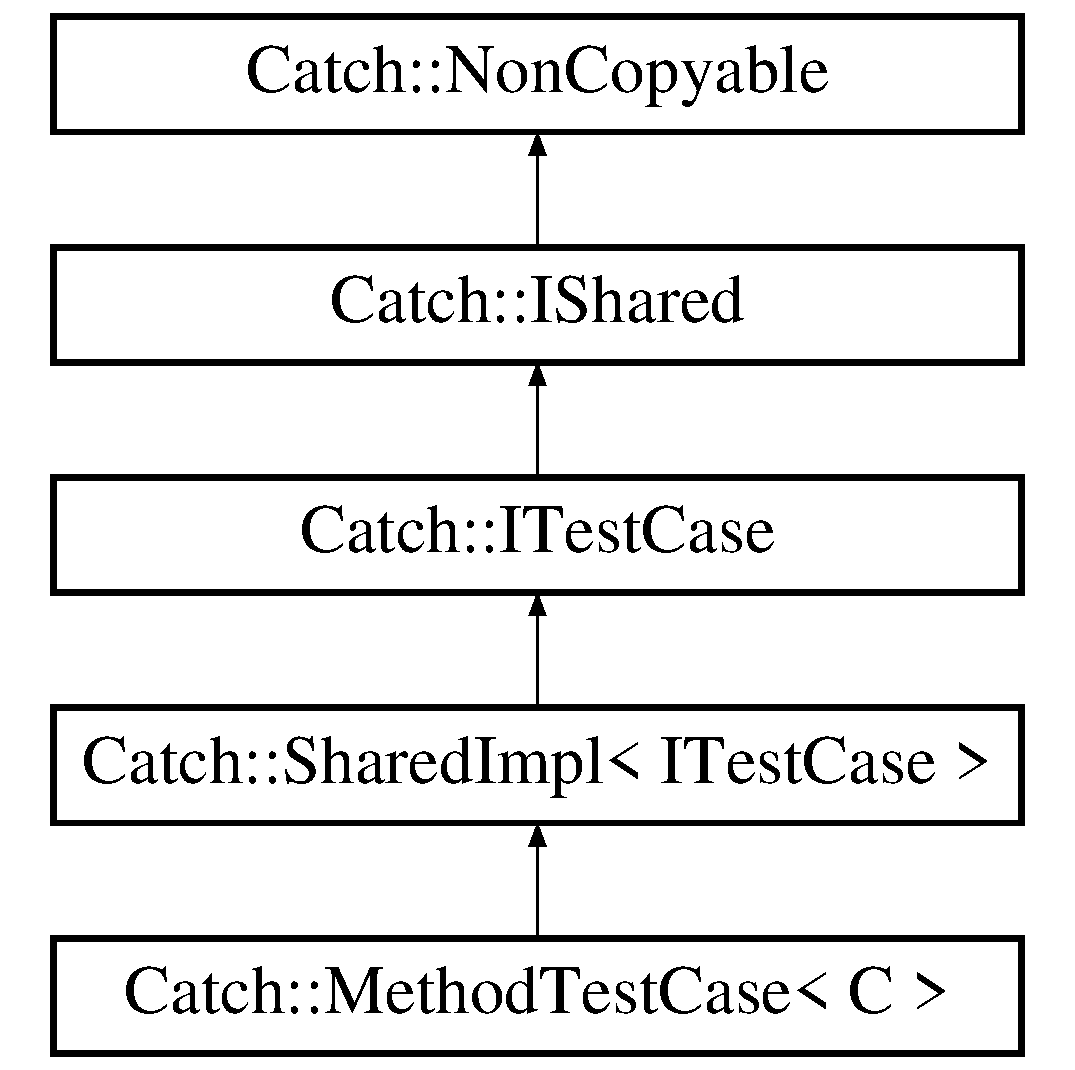
\includegraphics[height=5.000000cm]{struct_catch_1_1_i_shared}
\end{center}
\end{figure}
\subsection*{Public Member Functions}
\begin{DoxyCompactItemize}
\item 
virtual \mbox{\hyperlink{struct_catch_1_1_i_shared_a5e842e7540ae7ae0c62a2758123503f6}{$\sim$\+I\+Shared}} ()
\item 
virtual void \mbox{\hyperlink{struct_catch_1_1_i_shared_ae383df68557cdaf0910b411af04d9e33}{add\+Ref}} () const =0
\item 
virtual void \mbox{\hyperlink{struct_catch_1_1_i_shared_a002f52624728a763956fb6f230cb2f57}{release}} () const =0
\end{DoxyCompactItemize}
\subsection*{Additional Inherited Members}


\subsection{Constructor \& Destructor Documentation}
\mbox{\Hypertarget{struct_catch_1_1_i_shared_a5e842e7540ae7ae0c62a2758123503f6}\label{struct_catch_1_1_i_shared_a5e842e7540ae7ae0c62a2758123503f6}} 
\index{Catch\+::\+I\+Shared@{Catch\+::\+I\+Shared}!````~I\+Shared@{$\sim$\+I\+Shared}}
\index{````~I\+Shared@{$\sim$\+I\+Shared}!Catch\+::\+I\+Shared@{Catch\+::\+I\+Shared}}
\subsubsection{\texorpdfstring{$\sim$\+I\+Shared()}{~IShared()}}
{\footnotesize\ttfamily virtual Catch\+::\+I\+Shared\+::$\sim$\+I\+Shared (\begin{DoxyParamCaption}{ }\end{DoxyParamCaption})\hspace{0.3cm}{\ttfamily [virtual]}}



\subsection{Member Function Documentation}
\mbox{\Hypertarget{struct_catch_1_1_i_shared_ae383df68557cdaf0910b411af04d9e33}\label{struct_catch_1_1_i_shared_ae383df68557cdaf0910b411af04d9e33}} 
\index{Catch\+::\+I\+Shared@{Catch\+::\+I\+Shared}!add\+Ref@{add\+Ref}}
\index{add\+Ref@{add\+Ref}!Catch\+::\+I\+Shared@{Catch\+::\+I\+Shared}}
\subsubsection{\texorpdfstring{add\+Ref()}{addRef()}}
{\footnotesize\ttfamily virtual void Catch\+::\+I\+Shared\+::add\+Ref (\begin{DoxyParamCaption}{ }\end{DoxyParamCaption}) const\hspace{0.3cm}{\ttfamily [pure virtual]}}



Implemented in \mbox{\hyperlink{struct_catch_1_1_shared_impl_a5d1a4c96e8fc07c821890fd09749062e}{Catch\+::\+Shared\+Impl$<$ I\+Test\+Case $>$}}.

\mbox{\Hypertarget{struct_catch_1_1_i_shared_a002f52624728a763956fb6f230cb2f57}\label{struct_catch_1_1_i_shared_a002f52624728a763956fb6f230cb2f57}} 
\index{Catch\+::\+I\+Shared@{Catch\+::\+I\+Shared}!release@{release}}
\index{release@{release}!Catch\+::\+I\+Shared@{Catch\+::\+I\+Shared}}
\subsubsection{\texorpdfstring{release()}{release()}}
{\footnotesize\ttfamily virtual void Catch\+::\+I\+Shared\+::release (\begin{DoxyParamCaption}{ }\end{DoxyParamCaption}) const\hspace{0.3cm}{\ttfamily [pure virtual]}}



Implemented in \mbox{\hyperlink{struct_catch_1_1_shared_impl_ada8052c6f24fd73ec099333626f106fe}{Catch\+::\+Shared\+Impl$<$ I\+Test\+Case $>$}}.



The documentation for this struct was generated from the following file\+:\begin{DoxyCompactItemize}
\item 
include/\mbox{\hyperlink{catch_8hpp}{catch.\+hpp}}\end{DoxyCompactItemize}

\hypertarget{struct_catch_1_1_detail_1_1_is_stream_insertable}{}\section{Catch\+:\+:Detail\+:\+:Is\+Stream\+Insertable$<$ T $>$ Struct Template Reference}
\label{struct_catch_1_1_detail_1_1_is_stream_insertable}\index{Catch\+::\+Detail\+::\+Is\+Stream\+Insertable$<$ T $>$@{Catch\+::\+Detail\+::\+Is\+Stream\+Insertable$<$ T $>$}}


{\ttfamily \#include $<$catch.\+hpp$>$}

\subsection*{Public Types}
\begin{DoxyCompactItemize}
\item 
enum \{ \mbox{\hyperlink{struct_catch_1_1_detail_1_1_is_stream_insertable_a2e4508694da3bf368ff67733a7970edda765a324929702bfce2969fc19fc4f926}{value}} = sizeof( test\+Streamable(s $<$$<$ t) ) == sizeof( True\+Type )
 \}
\end{DoxyCompactItemize}
\subsection*{Static Public Attributes}
\begin{DoxyCompactItemize}
\item 
static std\+::ostream \& \mbox{\hyperlink{struct_catch_1_1_detail_1_1_is_stream_insertable_abe3d3c8e5d85665747faafffc9a96b00}{s}}
\item 
static T const  \& \mbox{\hyperlink{struct_catch_1_1_detail_1_1_is_stream_insertable_a7d2a3da978b6736667a7b2f6d51f507f}{t}}
\end{DoxyCompactItemize}


\subsection{Member Enumeration Documentation}
\mbox{\Hypertarget{struct_catch_1_1_detail_1_1_is_stream_insertable_a2e4508694da3bf368ff67733a7970edd}\label{struct_catch_1_1_detail_1_1_is_stream_insertable_a2e4508694da3bf368ff67733a7970edd}} 
\subsubsection{\texorpdfstring{anonymous enum}{anonymous enum}}
{\footnotesize\ttfamily template$<$typename T $>$ \\
anonymous enum}

\begin{DoxyEnumFields}{Enumerator}
\raisebox{\heightof{T}}[0pt][0pt]{\index{value@{value}!Catch\+::\+Detail\+::\+Is\+Stream\+Insertable@{Catch\+::\+Detail\+::\+Is\+Stream\+Insertable}}\index{Catch\+::\+Detail\+::\+Is\+Stream\+Insertable@{Catch\+::\+Detail\+::\+Is\+Stream\+Insertable}!value@{value}}}\mbox{\Hypertarget{struct_catch_1_1_detail_1_1_is_stream_insertable_a2e4508694da3bf368ff67733a7970edda765a324929702bfce2969fc19fc4f926}\label{struct_catch_1_1_detail_1_1_is_stream_insertable_a2e4508694da3bf368ff67733a7970edda765a324929702bfce2969fc19fc4f926}} 
value&\\
\hline

\end{DoxyEnumFields}


\subsection{Member Data Documentation}
\mbox{\Hypertarget{struct_catch_1_1_detail_1_1_is_stream_insertable_abe3d3c8e5d85665747faafffc9a96b00}\label{struct_catch_1_1_detail_1_1_is_stream_insertable_abe3d3c8e5d85665747faafffc9a96b00}} 
\index{Catch\+::\+Detail\+::\+Is\+Stream\+Insertable@{Catch\+::\+Detail\+::\+Is\+Stream\+Insertable}!s@{s}}
\index{s@{s}!Catch\+::\+Detail\+::\+Is\+Stream\+Insertable@{Catch\+::\+Detail\+::\+Is\+Stream\+Insertable}}
\subsubsection{\texorpdfstring{s}{s}}
{\footnotesize\ttfamily template$<$typename T $>$ \\
std\+::ostream\& \mbox{\hyperlink{struct_catch_1_1_detail_1_1_is_stream_insertable}{Catch\+::\+Detail\+::\+Is\+Stream\+Insertable}}$<$ T $>$\+::s\hspace{0.3cm}{\ttfamily [static]}}

\mbox{\Hypertarget{struct_catch_1_1_detail_1_1_is_stream_insertable_a7d2a3da978b6736667a7b2f6d51f507f}\label{struct_catch_1_1_detail_1_1_is_stream_insertable_a7d2a3da978b6736667a7b2f6d51f507f}} 
\index{Catch\+::\+Detail\+::\+Is\+Stream\+Insertable@{Catch\+::\+Detail\+::\+Is\+Stream\+Insertable}!t@{t}}
\index{t@{t}!Catch\+::\+Detail\+::\+Is\+Stream\+Insertable@{Catch\+::\+Detail\+::\+Is\+Stream\+Insertable}}
\subsubsection{\texorpdfstring{t}{t}}
{\footnotesize\ttfamily template$<$typename T $>$ \\
T const\& \mbox{\hyperlink{struct_catch_1_1_detail_1_1_is_stream_insertable}{Catch\+::\+Detail\+::\+Is\+Stream\+Insertable}}$<$ T $>$\+::t\hspace{0.3cm}{\ttfamily [static]}}



The documentation for this struct was generated from the following file\+:\begin{DoxyCompactItemize}
\item 
include/\mbox{\hyperlink{catch_8hpp}{catch.\+hpp}}\end{DoxyCompactItemize}

\hypertarget{struct_catch_1_1_i_tag_alias_registry}{}\section{Catch\+:\+:I\+Tag\+Alias\+Registry Struct Reference}
\label{struct_catch_1_1_i_tag_alias_registry}\index{Catch\+::\+I\+Tag\+Alias\+Registry@{Catch\+::\+I\+Tag\+Alias\+Registry}}


{\ttfamily \#include $<$catch.\+hpp$>$}

\subsection*{Public Member Functions}
\begin{DoxyCompactItemize}
\item 
virtual \mbox{\hyperlink{struct_catch_1_1_i_tag_alias_registry_a8967db4dd40b68e22697eff0f4928239}{$\sim$\+I\+Tag\+Alias\+Registry}} ()
\item 
virtual \mbox{\hyperlink{class_catch_1_1_option}{Option}}$<$ \mbox{\hyperlink{struct_catch_1_1_tag_alias}{Tag\+Alias}} $>$ \mbox{\hyperlink{struct_catch_1_1_i_tag_alias_registry_a7d2fba4d39cfcc62c2695fcde4f989c3}{find}} (std\+::string const \&alias) const =0
\item 
virtual std\+::string \mbox{\hyperlink{struct_catch_1_1_i_tag_alias_registry_ae729a7532faf7466db1a157ce0395170}{expand\+Aliases}} (std\+::string const \&unexpanded\+Test\+Spec) const =0
\end{DoxyCompactItemize}
\subsection*{Static Public Member Functions}
\begin{DoxyCompactItemize}
\item 
static \mbox{\hyperlink{struct_catch_1_1_i_tag_alias_registry}{I\+Tag\+Alias\+Registry}} const  \& \mbox{\hyperlink{struct_catch_1_1_i_tag_alias_registry_aa9d0f008f49473389c7abf6071f137a7}{get}} ()
\end{DoxyCompactItemize}


\subsection{Constructor \& Destructor Documentation}
\mbox{\Hypertarget{struct_catch_1_1_i_tag_alias_registry_a8967db4dd40b68e22697eff0f4928239}\label{struct_catch_1_1_i_tag_alias_registry_a8967db4dd40b68e22697eff0f4928239}} 
\index{Catch\+::\+I\+Tag\+Alias\+Registry@{Catch\+::\+I\+Tag\+Alias\+Registry}!````~I\+Tag\+Alias\+Registry@{$\sim$\+I\+Tag\+Alias\+Registry}}
\index{````~I\+Tag\+Alias\+Registry@{$\sim$\+I\+Tag\+Alias\+Registry}!Catch\+::\+I\+Tag\+Alias\+Registry@{Catch\+::\+I\+Tag\+Alias\+Registry}}
\subsubsection{\texorpdfstring{$\sim$\+I\+Tag\+Alias\+Registry()}{~ITagAliasRegistry()}}
{\footnotesize\ttfamily virtual Catch\+::\+I\+Tag\+Alias\+Registry\+::$\sim$\+I\+Tag\+Alias\+Registry (\begin{DoxyParamCaption}{ }\end{DoxyParamCaption})\hspace{0.3cm}{\ttfamily [virtual]}}



\subsection{Member Function Documentation}
\mbox{\Hypertarget{struct_catch_1_1_i_tag_alias_registry_ae729a7532faf7466db1a157ce0395170}\label{struct_catch_1_1_i_tag_alias_registry_ae729a7532faf7466db1a157ce0395170}} 
\index{Catch\+::\+I\+Tag\+Alias\+Registry@{Catch\+::\+I\+Tag\+Alias\+Registry}!expand\+Aliases@{expand\+Aliases}}
\index{expand\+Aliases@{expand\+Aliases}!Catch\+::\+I\+Tag\+Alias\+Registry@{Catch\+::\+I\+Tag\+Alias\+Registry}}
\subsubsection{\texorpdfstring{expand\+Aliases()}{expandAliases()}}
{\footnotesize\ttfamily virtual std\+::string Catch\+::\+I\+Tag\+Alias\+Registry\+::expand\+Aliases (\begin{DoxyParamCaption}\item[{std\+::string const \&}]{unexpanded\+Test\+Spec }\end{DoxyParamCaption}) const\hspace{0.3cm}{\ttfamily [pure virtual]}}

\mbox{\Hypertarget{struct_catch_1_1_i_tag_alias_registry_a7d2fba4d39cfcc62c2695fcde4f989c3}\label{struct_catch_1_1_i_tag_alias_registry_a7d2fba4d39cfcc62c2695fcde4f989c3}} 
\index{Catch\+::\+I\+Tag\+Alias\+Registry@{Catch\+::\+I\+Tag\+Alias\+Registry}!find@{find}}
\index{find@{find}!Catch\+::\+I\+Tag\+Alias\+Registry@{Catch\+::\+I\+Tag\+Alias\+Registry}}
\subsubsection{\texorpdfstring{find()}{find()}}
{\footnotesize\ttfamily virtual \mbox{\hyperlink{class_catch_1_1_option}{Option}}$<$\mbox{\hyperlink{struct_catch_1_1_tag_alias}{Tag\+Alias}}$>$ Catch\+::\+I\+Tag\+Alias\+Registry\+::find (\begin{DoxyParamCaption}\item[{std\+::string const \&}]{alias }\end{DoxyParamCaption}) const\hspace{0.3cm}{\ttfamily [pure virtual]}}

\mbox{\Hypertarget{struct_catch_1_1_i_tag_alias_registry_aa9d0f008f49473389c7abf6071f137a7}\label{struct_catch_1_1_i_tag_alias_registry_aa9d0f008f49473389c7abf6071f137a7}} 
\index{Catch\+::\+I\+Tag\+Alias\+Registry@{Catch\+::\+I\+Tag\+Alias\+Registry}!get@{get}}
\index{get@{get}!Catch\+::\+I\+Tag\+Alias\+Registry@{Catch\+::\+I\+Tag\+Alias\+Registry}}
\subsubsection{\texorpdfstring{get()}{get()}}
{\footnotesize\ttfamily static \mbox{\hyperlink{struct_catch_1_1_i_tag_alias_registry}{I\+Tag\+Alias\+Registry}} const\& Catch\+::\+I\+Tag\+Alias\+Registry\+::get (\begin{DoxyParamCaption}{ }\end{DoxyParamCaption})\hspace{0.3cm}{\ttfamily [static]}}



The documentation for this struct was generated from the following file\+:\begin{DoxyCompactItemize}
\item 
include/\mbox{\hyperlink{catch_8hpp}{catch.\+hpp}}\end{DoxyCompactItemize}

\hypertarget{struct_catch_1_1_i_test_case}{}\section{Catch\+:\+:I\+Test\+Case Struct Reference}
\label{struct_catch_1_1_i_test_case}\index{Catch\+::\+I\+Test\+Case@{Catch\+::\+I\+Test\+Case}}


{\ttfamily \#include $<$catch.\+hpp$>$}

Inheritance diagram for Catch\+:\+:I\+Test\+Case\+:\begin{figure}[H]
\begin{center}
\leavevmode
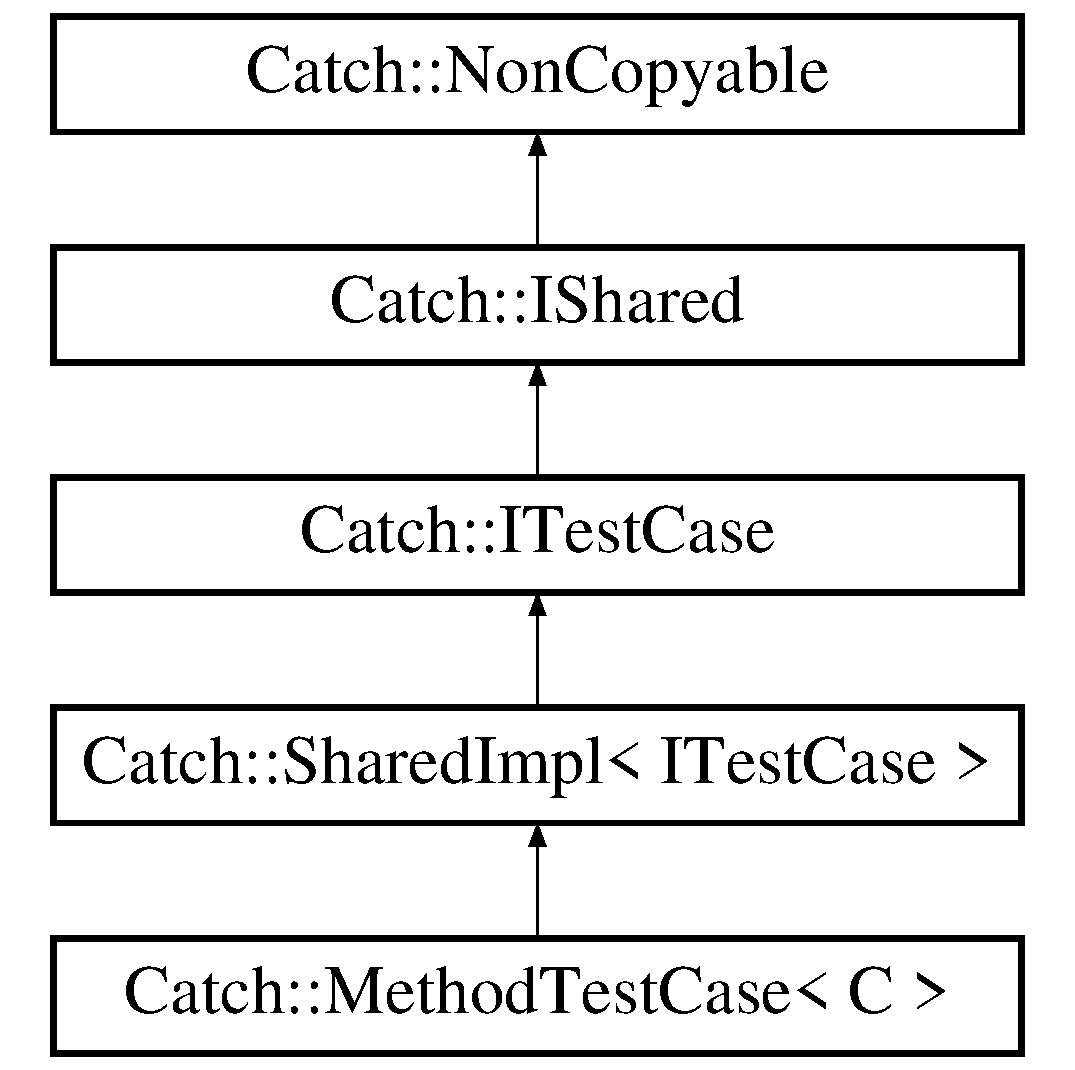
\includegraphics[height=5.000000cm]{struct_catch_1_1_i_test_case}
\end{center}
\end{figure}
\subsection*{Public Member Functions}
\begin{DoxyCompactItemize}
\item 
virtual void \mbox{\hyperlink{struct_catch_1_1_i_test_case_a678825e62e7c17297621cfeb65588c34}{invoke}} () const =0
\end{DoxyCompactItemize}
\subsection*{Protected Member Functions}
\begin{DoxyCompactItemize}
\item 
virtual \mbox{\hyperlink{struct_catch_1_1_i_test_case_add7b9bec455ac1b007c17df82144310e}{$\sim$\+I\+Test\+Case}} ()
\end{DoxyCompactItemize}


\subsection{Constructor \& Destructor Documentation}
\mbox{\Hypertarget{struct_catch_1_1_i_test_case_add7b9bec455ac1b007c17df82144310e}\label{struct_catch_1_1_i_test_case_add7b9bec455ac1b007c17df82144310e}} 
\index{Catch\+::\+I\+Test\+Case@{Catch\+::\+I\+Test\+Case}!````~I\+Test\+Case@{$\sim$\+I\+Test\+Case}}
\index{````~I\+Test\+Case@{$\sim$\+I\+Test\+Case}!Catch\+::\+I\+Test\+Case@{Catch\+::\+I\+Test\+Case}}
\subsubsection{\texorpdfstring{$\sim$\+I\+Test\+Case()}{~ITestCase()}}
{\footnotesize\ttfamily virtual Catch\+::\+I\+Test\+Case\+::$\sim$\+I\+Test\+Case (\begin{DoxyParamCaption}{ }\end{DoxyParamCaption})\hspace{0.3cm}{\ttfamily [protected]}, {\ttfamily [virtual]}}



\subsection{Member Function Documentation}
\mbox{\Hypertarget{struct_catch_1_1_i_test_case_a678825e62e7c17297621cfeb65588c34}\label{struct_catch_1_1_i_test_case_a678825e62e7c17297621cfeb65588c34}} 
\index{Catch\+::\+I\+Test\+Case@{Catch\+::\+I\+Test\+Case}!invoke@{invoke}}
\index{invoke@{invoke}!Catch\+::\+I\+Test\+Case@{Catch\+::\+I\+Test\+Case}}
\subsubsection{\texorpdfstring{invoke()}{invoke()}}
{\footnotesize\ttfamily virtual void Catch\+::\+I\+Test\+Case\+::invoke (\begin{DoxyParamCaption}{ }\end{DoxyParamCaption}) const\hspace{0.3cm}{\ttfamily [pure virtual]}}



Implemented in \mbox{\hyperlink{class_catch_1_1_method_test_case_a4e2263cfa0646f2980768328cb372793}{Catch\+::\+Method\+Test\+Case$<$ C $>$}}.



The documentation for this struct was generated from the following file\+:\begin{DoxyCompactItemize}
\item 
include/\mbox{\hyperlink{catch_8hpp}{catch.\+hpp}}\end{DoxyCompactItemize}

\hypertarget{struct_catch_1_1_i_test_case_registry}{}\section{Catch\+:\+:I\+Test\+Case\+Registry Struct Reference}
\label{struct_catch_1_1_i_test_case_registry}\index{Catch\+::\+I\+Test\+Case\+Registry@{Catch\+::\+I\+Test\+Case\+Registry}}


{\ttfamily \#include $<$catch.\+hpp$>$}

\subsection*{Public Member Functions}
\begin{DoxyCompactItemize}
\item 
virtual \mbox{\hyperlink{struct_catch_1_1_i_test_case_registry_ae14798f05ac8e2b18cff532849a4da81}{$\sim$\+I\+Test\+Case\+Registry}} ()
\item 
virtual std\+::vector$<$ \mbox{\hyperlink{class_catch_1_1_test_case}{Test\+Case}} $>$ const  \& \mbox{\hyperlink{struct_catch_1_1_i_test_case_registry_ad6e4d4a621655123f73ae98cfeda063d}{get\+All\+Tests}} () const =0
\item 
virtual std\+::vector$<$ \mbox{\hyperlink{class_catch_1_1_test_case}{Test\+Case}} $>$ const  \& \mbox{\hyperlink{struct_catch_1_1_i_test_case_registry_a33e46639d0319d35497c05bb5d02be5a}{get\+All\+Tests\+Sorted}} (I\+Config const \&config) const =0
\end{DoxyCompactItemize}


\subsection{Constructor \& Destructor Documentation}
\mbox{\Hypertarget{struct_catch_1_1_i_test_case_registry_ae14798f05ac8e2b18cff532849a4da81}\label{struct_catch_1_1_i_test_case_registry_ae14798f05ac8e2b18cff532849a4da81}} 
\index{Catch\+::\+I\+Test\+Case\+Registry@{Catch\+::\+I\+Test\+Case\+Registry}!````~I\+Test\+Case\+Registry@{$\sim$\+I\+Test\+Case\+Registry}}
\index{````~I\+Test\+Case\+Registry@{$\sim$\+I\+Test\+Case\+Registry}!Catch\+::\+I\+Test\+Case\+Registry@{Catch\+::\+I\+Test\+Case\+Registry}}
\subsubsection{\texorpdfstring{$\sim$\+I\+Test\+Case\+Registry()}{~ITestCaseRegistry()}}
{\footnotesize\ttfamily virtual Catch\+::\+I\+Test\+Case\+Registry\+::$\sim$\+I\+Test\+Case\+Registry (\begin{DoxyParamCaption}{ }\end{DoxyParamCaption})\hspace{0.3cm}{\ttfamily [virtual]}}



\subsection{Member Function Documentation}
\mbox{\Hypertarget{struct_catch_1_1_i_test_case_registry_ad6e4d4a621655123f73ae98cfeda063d}\label{struct_catch_1_1_i_test_case_registry_ad6e4d4a621655123f73ae98cfeda063d}} 
\index{Catch\+::\+I\+Test\+Case\+Registry@{Catch\+::\+I\+Test\+Case\+Registry}!get\+All\+Tests@{get\+All\+Tests}}
\index{get\+All\+Tests@{get\+All\+Tests}!Catch\+::\+I\+Test\+Case\+Registry@{Catch\+::\+I\+Test\+Case\+Registry}}
\subsubsection{\texorpdfstring{get\+All\+Tests()}{getAllTests()}}
{\footnotesize\ttfamily virtual std\+::vector$<$\mbox{\hyperlink{class_catch_1_1_test_case}{Test\+Case}}$>$ const\& Catch\+::\+I\+Test\+Case\+Registry\+::get\+All\+Tests (\begin{DoxyParamCaption}{ }\end{DoxyParamCaption}) const\hspace{0.3cm}{\ttfamily [pure virtual]}}

\mbox{\Hypertarget{struct_catch_1_1_i_test_case_registry_a33e46639d0319d35497c05bb5d02be5a}\label{struct_catch_1_1_i_test_case_registry_a33e46639d0319d35497c05bb5d02be5a}} 
\index{Catch\+::\+I\+Test\+Case\+Registry@{Catch\+::\+I\+Test\+Case\+Registry}!get\+All\+Tests\+Sorted@{get\+All\+Tests\+Sorted}}
\index{get\+All\+Tests\+Sorted@{get\+All\+Tests\+Sorted}!Catch\+::\+I\+Test\+Case\+Registry@{Catch\+::\+I\+Test\+Case\+Registry}}
\subsubsection{\texorpdfstring{get\+All\+Tests\+Sorted()}{getAllTestsSorted()}}
{\footnotesize\ttfamily virtual std\+::vector$<$\mbox{\hyperlink{class_catch_1_1_test_case}{Test\+Case}}$>$ const\& Catch\+::\+I\+Test\+Case\+Registry\+::get\+All\+Tests\+Sorted (\begin{DoxyParamCaption}\item[{I\+Config const \&}]{config }\end{DoxyParamCaption}) const\hspace{0.3cm}{\ttfamily [pure virtual]}}



The documentation for this struct was generated from the following file\+:\begin{DoxyCompactItemize}
\item 
include/\mbox{\hyperlink{catch_8hpp}{catch.\+hpp}}\end{DoxyCompactItemize}

\hypertarget{struct_catch_1_1_matchers_1_1_impl_1_1_match_all_of}{}\section{Catch\+:\+:Matchers\+:\+:Impl\+:\+:Match\+All\+Of$<$ ArgT $>$ Struct Template Reference}
\label{struct_catch_1_1_matchers_1_1_impl_1_1_match_all_of}\index{Catch\+::\+Matchers\+::\+Impl\+::\+Match\+All\+Of$<$ Arg\+T $>$@{Catch\+::\+Matchers\+::\+Impl\+::\+Match\+All\+Of$<$ Arg\+T $>$}}


{\ttfamily \#include $<$catch.\+hpp$>$}

Inheritance diagram for Catch\+:\+:Matchers\+:\+:Impl\+:\+:Match\+All\+Of$<$ ArgT $>$\+:\begin{figure}[H]
\begin{center}
\leavevmode
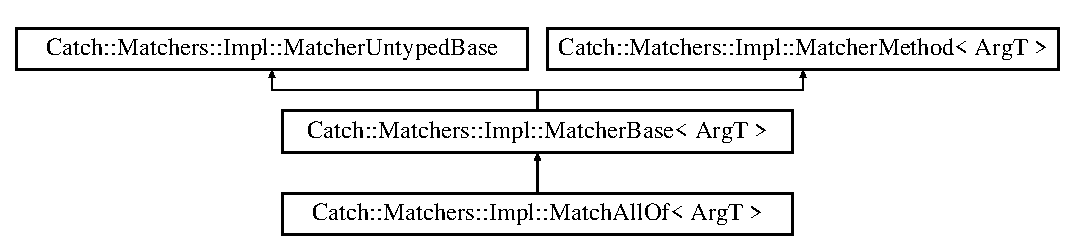
\includegraphics[height=2.926829cm]{struct_catch_1_1_matchers_1_1_impl_1_1_match_all_of}
\end{center}
\end{figure}
\subsection*{Public Member Functions}
\begin{DoxyCompactItemize}
\item 
virtual bool \mbox{\hyperlink{struct_catch_1_1_matchers_1_1_impl_1_1_match_all_of_a7bf0c2d8cedf67ecf9d0a527cb5a8263}{match}} (ArgT const \&arg) const \mbox{\hyperlink{catch_8hpp_a8ecdce4d3f57835f707915ae831eb847}{C\+A\+T\+C\+H\+\_\+\+O\+V\+E\+R\+R\+I\+DE}}
\item 
virtual std\+::string \mbox{\hyperlink{struct_catch_1_1_matchers_1_1_impl_1_1_match_all_of_aaefeba99a0b35425203468a65bff544b}{describe}} () const \mbox{\hyperlink{catch_8hpp_a8ecdce4d3f57835f707915ae831eb847}{C\+A\+T\+C\+H\+\_\+\+O\+V\+E\+R\+R\+I\+DE}}
\item 
\mbox{\hyperlink{struct_catch_1_1_matchers_1_1_impl_1_1_match_all_of}{Match\+All\+Of}}$<$ ArgT $>$ \& \mbox{\hyperlink{struct_catch_1_1_matchers_1_1_impl_1_1_match_all_of_a9d0e38b36474336498d627610db434f3}{operator\&\&}} (\mbox{\hyperlink{struct_catch_1_1_matchers_1_1_impl_1_1_matcher_base}{Matcher\+Base}}$<$ ArgT $>$ const \&other)
\end{DoxyCompactItemize}
\subsection*{Public Attributes}
\begin{DoxyCompactItemize}
\item 
std\+::vector$<$ \mbox{\hyperlink{struct_catch_1_1_matchers_1_1_impl_1_1_matcher_base}{Matcher\+Base}}$<$ ArgT $>$ const  $\ast$ $>$ \mbox{\hyperlink{struct_catch_1_1_matchers_1_1_impl_1_1_match_all_of_a98d6a2611f195a4a5c49f92fd877be9a}{m\+\_\+matchers}}
\end{DoxyCompactItemize}
\subsection*{Additional Inherited Members}


\subsection{Member Function Documentation}
\mbox{\Hypertarget{struct_catch_1_1_matchers_1_1_impl_1_1_match_all_of_aaefeba99a0b35425203468a65bff544b}\label{struct_catch_1_1_matchers_1_1_impl_1_1_match_all_of_aaefeba99a0b35425203468a65bff544b}} 
\index{Catch\+::\+Matchers\+::\+Impl\+::\+Match\+All\+Of@{Catch\+::\+Matchers\+::\+Impl\+::\+Match\+All\+Of}!describe@{describe}}
\index{describe@{describe}!Catch\+::\+Matchers\+::\+Impl\+::\+Match\+All\+Of@{Catch\+::\+Matchers\+::\+Impl\+::\+Match\+All\+Of}}
\subsubsection{\texorpdfstring{describe()}{describe()}}
{\footnotesize\ttfamily template$<$typename ArgT$>$ \\
virtual std\+::string \mbox{\hyperlink{struct_catch_1_1_matchers_1_1_impl_1_1_match_all_of}{Catch\+::\+Matchers\+::\+Impl\+::\+Match\+All\+Of}}$<$ ArgT $>$\+::describe (\begin{DoxyParamCaption}{ }\end{DoxyParamCaption}) const\hspace{0.3cm}{\ttfamily [inline]}, {\ttfamily [virtual]}}



Implements \mbox{\hyperlink{class_catch_1_1_matchers_1_1_impl_1_1_matcher_untyped_base_a91d3a907dbfcbb596077df24f6e11fe2}{Catch\+::\+Matchers\+::\+Impl\+::\+Matcher\+Untyped\+Base}}.

\mbox{\Hypertarget{struct_catch_1_1_matchers_1_1_impl_1_1_match_all_of_a7bf0c2d8cedf67ecf9d0a527cb5a8263}\label{struct_catch_1_1_matchers_1_1_impl_1_1_match_all_of_a7bf0c2d8cedf67ecf9d0a527cb5a8263}} 
\index{Catch\+::\+Matchers\+::\+Impl\+::\+Match\+All\+Of@{Catch\+::\+Matchers\+::\+Impl\+::\+Match\+All\+Of}!match@{match}}
\index{match@{match}!Catch\+::\+Matchers\+::\+Impl\+::\+Match\+All\+Of@{Catch\+::\+Matchers\+::\+Impl\+::\+Match\+All\+Of}}
\subsubsection{\texorpdfstring{match()}{match()}}
{\footnotesize\ttfamily template$<$typename ArgT$>$ \\
virtual bool \mbox{\hyperlink{struct_catch_1_1_matchers_1_1_impl_1_1_match_all_of}{Catch\+::\+Matchers\+::\+Impl\+::\+Match\+All\+Of}}$<$ ArgT $>$\+::match (\begin{DoxyParamCaption}\item[{ArgT const \&}]{arg }\end{DoxyParamCaption}) const\hspace{0.3cm}{\ttfamily [inline]}, {\ttfamily [virtual]}}



Implements \mbox{\hyperlink{struct_catch_1_1_matchers_1_1_impl_1_1_matcher_method_ae0920ff9e817acf08e1bb0cbcb044e30}{Catch\+::\+Matchers\+::\+Impl\+::\+Matcher\+Method$<$ Arg\+T $>$}}.

\mbox{\Hypertarget{struct_catch_1_1_matchers_1_1_impl_1_1_match_all_of_a9d0e38b36474336498d627610db434f3}\label{struct_catch_1_1_matchers_1_1_impl_1_1_match_all_of_a9d0e38b36474336498d627610db434f3}} 
\index{Catch\+::\+Matchers\+::\+Impl\+::\+Match\+All\+Of@{Catch\+::\+Matchers\+::\+Impl\+::\+Match\+All\+Of}!operator\&\&@{operator\&\&}}
\index{operator\&\&@{operator\&\&}!Catch\+::\+Matchers\+::\+Impl\+::\+Match\+All\+Of@{Catch\+::\+Matchers\+::\+Impl\+::\+Match\+All\+Of}}
\subsubsection{\texorpdfstring{operator\&\&()}{operator\&\&()}}
{\footnotesize\ttfamily template$<$typename ArgT$>$ \\
\mbox{\hyperlink{struct_catch_1_1_matchers_1_1_impl_1_1_match_all_of}{Match\+All\+Of}}$<$ArgT$>$\& \mbox{\hyperlink{struct_catch_1_1_matchers_1_1_impl_1_1_match_all_of}{Catch\+::\+Matchers\+::\+Impl\+::\+Match\+All\+Of}}$<$ ArgT $>$\+::operator \&\& (\begin{DoxyParamCaption}\item[{\mbox{\hyperlink{struct_catch_1_1_matchers_1_1_impl_1_1_matcher_base}{Matcher\+Base}}$<$ ArgT $>$ const \&}]{other }\end{DoxyParamCaption})\hspace{0.3cm}{\ttfamily [inline]}}



\subsection{Member Data Documentation}
\mbox{\Hypertarget{struct_catch_1_1_matchers_1_1_impl_1_1_match_all_of_a98d6a2611f195a4a5c49f92fd877be9a}\label{struct_catch_1_1_matchers_1_1_impl_1_1_match_all_of_a98d6a2611f195a4a5c49f92fd877be9a}} 
\index{Catch\+::\+Matchers\+::\+Impl\+::\+Match\+All\+Of@{Catch\+::\+Matchers\+::\+Impl\+::\+Match\+All\+Of}!m\+\_\+matchers@{m\+\_\+matchers}}
\index{m\+\_\+matchers@{m\+\_\+matchers}!Catch\+::\+Matchers\+::\+Impl\+::\+Match\+All\+Of@{Catch\+::\+Matchers\+::\+Impl\+::\+Match\+All\+Of}}
\subsubsection{\texorpdfstring{m\+\_\+matchers}{m\_matchers}}
{\footnotesize\ttfamily template$<$typename ArgT$>$ \\
std\+::vector$<$\mbox{\hyperlink{struct_catch_1_1_matchers_1_1_impl_1_1_matcher_base}{Matcher\+Base}}$<$ArgT$>$ const$\ast$$>$ \mbox{\hyperlink{struct_catch_1_1_matchers_1_1_impl_1_1_match_all_of}{Catch\+::\+Matchers\+::\+Impl\+::\+Match\+All\+Of}}$<$ ArgT $>$\+::m\+\_\+matchers}



The documentation for this struct was generated from the following file\+:\begin{DoxyCompactItemize}
\item 
include/\mbox{\hyperlink{catch_8hpp}{catch.\+hpp}}\end{DoxyCompactItemize}

\hypertarget{struct_catch_1_1_matchers_1_1_impl_1_1_match_any_of}{}\section{Catch\+:\+:Matchers\+:\+:Impl\+:\+:Match\+Any\+Of$<$ ArgT $>$ Struct Template Reference}
\label{struct_catch_1_1_matchers_1_1_impl_1_1_match_any_of}\index{Catch\+::\+Matchers\+::\+Impl\+::\+Match\+Any\+Of$<$ Arg\+T $>$@{Catch\+::\+Matchers\+::\+Impl\+::\+Match\+Any\+Of$<$ Arg\+T $>$}}


{\ttfamily \#include $<$catch.\+hpp$>$}

Inheritance diagram for Catch\+:\+:Matchers\+:\+:Impl\+:\+:Match\+Any\+Of$<$ ArgT $>$\+:\begin{figure}[H]
\begin{center}
\leavevmode
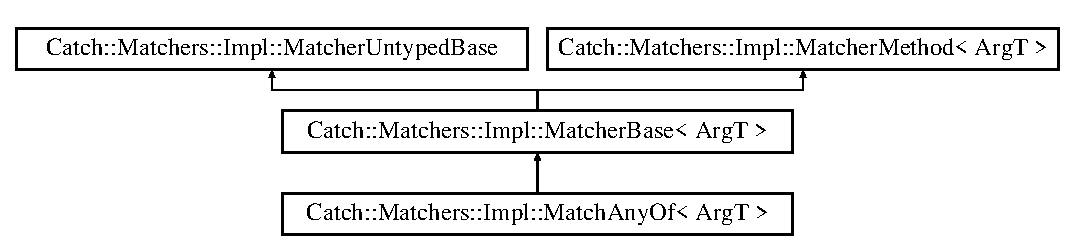
\includegraphics[height=2.926829cm]{struct_catch_1_1_matchers_1_1_impl_1_1_match_any_of}
\end{center}
\end{figure}
\subsection*{Public Member Functions}
\begin{DoxyCompactItemize}
\item 
virtual bool \mbox{\hyperlink{struct_catch_1_1_matchers_1_1_impl_1_1_match_any_of_a73be317ecf5919af855af96d68e714b9}{match}} (ArgT const \&arg) const \mbox{\hyperlink{catch_8hpp_a8ecdce4d3f57835f707915ae831eb847}{C\+A\+T\+C\+H\+\_\+\+O\+V\+E\+R\+R\+I\+DE}}
\item 
virtual std\+::string \mbox{\hyperlink{struct_catch_1_1_matchers_1_1_impl_1_1_match_any_of_a020f5d7889d8cd8be9ad309c690147b6}{describe}} () const \mbox{\hyperlink{catch_8hpp_a8ecdce4d3f57835f707915ae831eb847}{C\+A\+T\+C\+H\+\_\+\+O\+V\+E\+R\+R\+I\+DE}}
\item 
\mbox{\hyperlink{struct_catch_1_1_matchers_1_1_impl_1_1_match_any_of}{Match\+Any\+Of}}$<$ ArgT $>$ \& \mbox{\hyperlink{struct_catch_1_1_matchers_1_1_impl_1_1_match_any_of_a44d7582dbe09fc31b9a5ba8a6367b506}{operator$\vert$$\vert$}} (\mbox{\hyperlink{struct_catch_1_1_matchers_1_1_impl_1_1_matcher_base}{Matcher\+Base}}$<$ ArgT $>$ const \&other)
\end{DoxyCompactItemize}
\subsection*{Public Attributes}
\begin{DoxyCompactItemize}
\item 
std\+::vector$<$ \mbox{\hyperlink{struct_catch_1_1_matchers_1_1_impl_1_1_matcher_base}{Matcher\+Base}}$<$ ArgT $>$ const  $\ast$ $>$ \mbox{\hyperlink{struct_catch_1_1_matchers_1_1_impl_1_1_match_any_of_a1fb1119e6110dc15b8d5262ec0aeddd5}{m\+\_\+matchers}}
\end{DoxyCompactItemize}
\subsection*{Additional Inherited Members}


\subsection{Member Function Documentation}
\mbox{\Hypertarget{struct_catch_1_1_matchers_1_1_impl_1_1_match_any_of_a020f5d7889d8cd8be9ad309c690147b6}\label{struct_catch_1_1_matchers_1_1_impl_1_1_match_any_of_a020f5d7889d8cd8be9ad309c690147b6}} 
\index{Catch\+::\+Matchers\+::\+Impl\+::\+Match\+Any\+Of@{Catch\+::\+Matchers\+::\+Impl\+::\+Match\+Any\+Of}!describe@{describe}}
\index{describe@{describe}!Catch\+::\+Matchers\+::\+Impl\+::\+Match\+Any\+Of@{Catch\+::\+Matchers\+::\+Impl\+::\+Match\+Any\+Of}}
\subsubsection{\texorpdfstring{describe()}{describe()}}
{\footnotesize\ttfamily template$<$typename ArgT$>$ \\
virtual std\+::string \mbox{\hyperlink{struct_catch_1_1_matchers_1_1_impl_1_1_match_any_of}{Catch\+::\+Matchers\+::\+Impl\+::\+Match\+Any\+Of}}$<$ ArgT $>$\+::describe (\begin{DoxyParamCaption}{ }\end{DoxyParamCaption}) const\hspace{0.3cm}{\ttfamily [inline]}, {\ttfamily [virtual]}}



Implements \mbox{\hyperlink{class_catch_1_1_matchers_1_1_impl_1_1_matcher_untyped_base_a91d3a907dbfcbb596077df24f6e11fe2}{Catch\+::\+Matchers\+::\+Impl\+::\+Matcher\+Untyped\+Base}}.

\mbox{\Hypertarget{struct_catch_1_1_matchers_1_1_impl_1_1_match_any_of_a73be317ecf5919af855af96d68e714b9}\label{struct_catch_1_1_matchers_1_1_impl_1_1_match_any_of_a73be317ecf5919af855af96d68e714b9}} 
\index{Catch\+::\+Matchers\+::\+Impl\+::\+Match\+Any\+Of@{Catch\+::\+Matchers\+::\+Impl\+::\+Match\+Any\+Of}!match@{match}}
\index{match@{match}!Catch\+::\+Matchers\+::\+Impl\+::\+Match\+Any\+Of@{Catch\+::\+Matchers\+::\+Impl\+::\+Match\+Any\+Of}}
\subsubsection{\texorpdfstring{match()}{match()}}
{\footnotesize\ttfamily template$<$typename ArgT$>$ \\
virtual bool \mbox{\hyperlink{struct_catch_1_1_matchers_1_1_impl_1_1_match_any_of}{Catch\+::\+Matchers\+::\+Impl\+::\+Match\+Any\+Of}}$<$ ArgT $>$\+::match (\begin{DoxyParamCaption}\item[{ArgT const \&}]{arg }\end{DoxyParamCaption}) const\hspace{0.3cm}{\ttfamily [inline]}, {\ttfamily [virtual]}}



Implements \mbox{\hyperlink{struct_catch_1_1_matchers_1_1_impl_1_1_matcher_method_ae0920ff9e817acf08e1bb0cbcb044e30}{Catch\+::\+Matchers\+::\+Impl\+::\+Matcher\+Method$<$ Arg\+T $>$}}.

\mbox{\Hypertarget{struct_catch_1_1_matchers_1_1_impl_1_1_match_any_of_a44d7582dbe09fc31b9a5ba8a6367b506}\label{struct_catch_1_1_matchers_1_1_impl_1_1_match_any_of_a44d7582dbe09fc31b9a5ba8a6367b506}} 
\index{Catch\+::\+Matchers\+::\+Impl\+::\+Match\+Any\+Of@{Catch\+::\+Matchers\+::\+Impl\+::\+Match\+Any\+Of}!operator\texttt{"|}\texttt{"|}@{operator\texttt{"|}\texttt{"|}}}
\index{operator\texttt{"|}\texttt{"|}@{operator\texttt{"|}\texttt{"|}}!Catch\+::\+Matchers\+::\+Impl\+::\+Match\+Any\+Of@{Catch\+::\+Matchers\+::\+Impl\+::\+Match\+Any\+Of}}
\subsubsection{\texorpdfstring{operator\texttt{"|}\texttt{"|}()}{operator||()}}
{\footnotesize\ttfamily template$<$typename ArgT$>$ \\
\mbox{\hyperlink{struct_catch_1_1_matchers_1_1_impl_1_1_match_any_of}{Match\+Any\+Of}}$<$ArgT$>$\& \mbox{\hyperlink{struct_catch_1_1_matchers_1_1_impl_1_1_match_any_of}{Catch\+::\+Matchers\+::\+Impl\+::\+Match\+Any\+Of}}$<$ ArgT $>$\+::operator$\vert$$\vert$ (\begin{DoxyParamCaption}\item[{\mbox{\hyperlink{struct_catch_1_1_matchers_1_1_impl_1_1_matcher_base}{Matcher\+Base}}$<$ ArgT $>$ const \&}]{other }\end{DoxyParamCaption})\hspace{0.3cm}{\ttfamily [inline]}}



\subsection{Member Data Documentation}
\mbox{\Hypertarget{struct_catch_1_1_matchers_1_1_impl_1_1_match_any_of_a1fb1119e6110dc15b8d5262ec0aeddd5}\label{struct_catch_1_1_matchers_1_1_impl_1_1_match_any_of_a1fb1119e6110dc15b8d5262ec0aeddd5}} 
\index{Catch\+::\+Matchers\+::\+Impl\+::\+Match\+Any\+Of@{Catch\+::\+Matchers\+::\+Impl\+::\+Match\+Any\+Of}!m\+\_\+matchers@{m\+\_\+matchers}}
\index{m\+\_\+matchers@{m\+\_\+matchers}!Catch\+::\+Matchers\+::\+Impl\+::\+Match\+Any\+Of@{Catch\+::\+Matchers\+::\+Impl\+::\+Match\+Any\+Of}}
\subsubsection{\texorpdfstring{m\+\_\+matchers}{m\_matchers}}
{\footnotesize\ttfamily template$<$typename ArgT$>$ \\
std\+::vector$<$\mbox{\hyperlink{struct_catch_1_1_matchers_1_1_impl_1_1_matcher_base}{Matcher\+Base}}$<$ArgT$>$ const$\ast$$>$ \mbox{\hyperlink{struct_catch_1_1_matchers_1_1_impl_1_1_match_any_of}{Catch\+::\+Matchers\+::\+Impl\+::\+Match\+Any\+Of}}$<$ ArgT $>$\+::m\+\_\+matchers}



The documentation for this struct was generated from the following file\+:\begin{DoxyCompactItemize}
\item 
include/\mbox{\hyperlink{catch_8hpp}{catch.\+hpp}}\end{DoxyCompactItemize}

\hypertarget{struct_catch_1_1_matchers_1_1_impl_1_1_matcher_base}{}\section{Catch\+:\+:Matchers\+:\+:Impl\+:\+:Matcher\+Base$<$ ObjectT, ComparatorT $>$ Struct Template Reference}
\label{struct_catch_1_1_matchers_1_1_impl_1_1_matcher_base}\index{Catch\+::\+Matchers\+::\+Impl\+::\+Matcher\+Base$<$ Object\+T, Comparator\+T $>$@{Catch\+::\+Matchers\+::\+Impl\+::\+Matcher\+Base$<$ Object\+T, Comparator\+T $>$}}


{\ttfamily \#include $<$catch.\+hpp$>$}

Inheritance diagram for Catch\+:\+:Matchers\+:\+:Impl\+:\+:Matcher\+Base$<$ ObjectT, ComparatorT $>$\+:\begin{figure}[H]
\begin{center}
\leavevmode
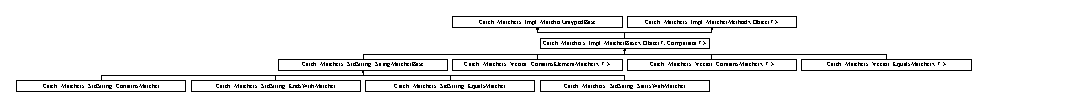
\includegraphics[height=1.006289cm]{struct_catch_1_1_matchers_1_1_impl_1_1_matcher_base}
\end{center}
\end{figure}
\subsection*{Public Member Functions}
\begin{DoxyCompactItemize}
\item 
\mbox{\hyperlink{struct_catch_1_1_matchers_1_1_impl_1_1_match_all_of}{Match\+All\+Of}}$<$ ComparatorT $>$ \mbox{\hyperlink{struct_catch_1_1_matchers_1_1_impl_1_1_matcher_base_a3deede6b29d20c15cb5efc79df40a520}{operator\&\&}} (\mbox{\hyperlink{struct_catch_1_1_matchers_1_1_impl_1_1_matcher_base}{Matcher\+Base}} const \&other) const
\item 
\mbox{\hyperlink{struct_catch_1_1_matchers_1_1_impl_1_1_match_any_of}{Match\+Any\+Of}}$<$ ComparatorT $>$ \mbox{\hyperlink{struct_catch_1_1_matchers_1_1_impl_1_1_matcher_base_ae0345ee76d109ac6d0241be261450ebc}{operator$\vert$$\vert$}} (\mbox{\hyperlink{struct_catch_1_1_matchers_1_1_impl_1_1_matcher_base}{Matcher\+Base}} const \&other) const
\item 
\mbox{\hyperlink{struct_catch_1_1_matchers_1_1_impl_1_1_match_not_of}{Match\+Not\+Of}}$<$ ComparatorT $>$ \mbox{\hyperlink{struct_catch_1_1_matchers_1_1_impl_1_1_matcher_base_a85174b5b27113f7bdc47c140c1c72602}{operator!}} () const
\end{DoxyCompactItemize}
\subsection*{Additional Inherited Members}


\subsection{Member Function Documentation}
\mbox{\Hypertarget{struct_catch_1_1_matchers_1_1_impl_1_1_matcher_base_a85174b5b27113f7bdc47c140c1c72602}\label{struct_catch_1_1_matchers_1_1_impl_1_1_matcher_base_a85174b5b27113f7bdc47c140c1c72602}} 
\index{Catch\+::\+Matchers\+::\+Impl\+::\+Matcher\+Base@{Catch\+::\+Matchers\+::\+Impl\+::\+Matcher\+Base}!operator"!@{operator"!}}
\index{operator"!@{operator"!}!Catch\+::\+Matchers\+::\+Impl\+::\+Matcher\+Base@{Catch\+::\+Matchers\+::\+Impl\+::\+Matcher\+Base}}
\subsubsection{\texorpdfstring{operator"!()}{operator!()}}
{\footnotesize\ttfamily template$<$typename ObjectT , typename ComparatorT $>$ \\
\mbox{\hyperlink{struct_catch_1_1_matchers_1_1_impl_1_1_match_not_of}{Match\+Not\+Of}}$<$ ComparatorT $>$ \mbox{\hyperlink{struct_catch_1_1_matchers_1_1_impl_1_1_matcher_base}{Catch\+::\+Matchers\+::\+Impl\+::\+Matcher\+Base}}$<$ ObjectT, ComparatorT $>$\+::operator! (\begin{DoxyParamCaption}{ }\end{DoxyParamCaption}) const}

\mbox{\Hypertarget{struct_catch_1_1_matchers_1_1_impl_1_1_matcher_base_a3deede6b29d20c15cb5efc79df40a520}\label{struct_catch_1_1_matchers_1_1_impl_1_1_matcher_base_a3deede6b29d20c15cb5efc79df40a520}} 
\index{Catch\+::\+Matchers\+::\+Impl\+::\+Matcher\+Base@{Catch\+::\+Matchers\+::\+Impl\+::\+Matcher\+Base}!operator\&\&@{operator\&\&}}
\index{operator\&\&@{operator\&\&}!Catch\+::\+Matchers\+::\+Impl\+::\+Matcher\+Base@{Catch\+::\+Matchers\+::\+Impl\+::\+Matcher\+Base}}
\subsubsection{\texorpdfstring{operator\&\&()}{operator\&\&()}}
{\footnotesize\ttfamily template$<$typename ObjectT, typename ComparatorT = ObjectT$>$ \\
\mbox{\hyperlink{struct_catch_1_1_matchers_1_1_impl_1_1_match_all_of}{Match\+All\+Of}}$<$ComparatorT$>$ \mbox{\hyperlink{struct_catch_1_1_matchers_1_1_impl_1_1_matcher_base}{Catch\+::\+Matchers\+::\+Impl\+::\+Matcher\+Base}}$<$ ObjectT, ComparatorT $>$\+::operator \&\& (\begin{DoxyParamCaption}\item[{\mbox{\hyperlink{struct_catch_1_1_matchers_1_1_impl_1_1_matcher_base}{Matcher\+Base}}$<$ ObjectT, ComparatorT $>$ const \&}]{other }\end{DoxyParamCaption}) const}

\mbox{\Hypertarget{struct_catch_1_1_matchers_1_1_impl_1_1_matcher_base_ae0345ee76d109ac6d0241be261450ebc}\label{struct_catch_1_1_matchers_1_1_impl_1_1_matcher_base_ae0345ee76d109ac6d0241be261450ebc}} 
\index{Catch\+::\+Matchers\+::\+Impl\+::\+Matcher\+Base@{Catch\+::\+Matchers\+::\+Impl\+::\+Matcher\+Base}!operator\texttt{"|}\texttt{"|}@{operator\texttt{"|}\texttt{"|}}}
\index{operator\texttt{"|}\texttt{"|}@{operator\texttt{"|}\texttt{"|}}!Catch\+::\+Matchers\+::\+Impl\+::\+Matcher\+Base@{Catch\+::\+Matchers\+::\+Impl\+::\+Matcher\+Base}}
\subsubsection{\texorpdfstring{operator\texttt{"|}\texttt{"|}()}{operator||()}}
{\footnotesize\ttfamily template$<$typename ObjectT , typename ComparatorT $>$ \\
\mbox{\hyperlink{struct_catch_1_1_matchers_1_1_impl_1_1_match_any_of}{Match\+Any\+Of}}$<$ ComparatorT $>$ \mbox{\hyperlink{struct_catch_1_1_matchers_1_1_impl_1_1_matcher_base}{Catch\+::\+Matchers\+::\+Impl\+::\+Matcher\+Base}}$<$ ObjectT, ComparatorT $>$\+::operator$\vert$$\vert$ (\begin{DoxyParamCaption}\item[{\mbox{\hyperlink{struct_catch_1_1_matchers_1_1_impl_1_1_matcher_base}{Matcher\+Base}}$<$ ObjectT, ComparatorT $>$ const \&}]{other }\end{DoxyParamCaption}) const}



The documentation for this struct was generated from the following file\+:\begin{DoxyCompactItemize}
\item 
include/\mbox{\hyperlink{catch_8hpp}{catch.\+hpp}}\end{DoxyCompactItemize}

\hypertarget{struct_catch_1_1_matchers_1_1_impl_1_1_matcher_method}{}\section{Catch\+:\+:Matchers\+:\+:Impl\+:\+:Matcher\+Method$<$ ObjectT $>$ Struct Template Reference}
\label{struct_catch_1_1_matchers_1_1_impl_1_1_matcher_method}\index{Catch\+::\+Matchers\+::\+Impl\+::\+Matcher\+Method$<$ Object\+T $>$@{Catch\+::\+Matchers\+::\+Impl\+::\+Matcher\+Method$<$ Object\+T $>$}}


{\ttfamily \#include $<$catch.\+hpp$>$}

Inheritance diagram for Catch\+:\+:Matchers\+:\+:Impl\+:\+:Matcher\+Method$<$ ObjectT $>$\+:\begin{figure}[H]
\begin{center}
\leavevmode
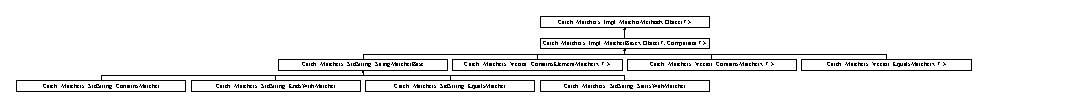
\includegraphics[height=1.006289cm]{struct_catch_1_1_matchers_1_1_impl_1_1_matcher_method}
\end{center}
\end{figure}
\subsection*{Public Member Functions}
\begin{DoxyCompactItemize}
\item 
virtual bool \mbox{\hyperlink{struct_catch_1_1_matchers_1_1_impl_1_1_matcher_method_ae0920ff9e817acf08e1bb0cbcb044e30}{match}} (ObjectT const \&arg) const =0
\end{DoxyCompactItemize}


\subsection{Member Function Documentation}
\mbox{\Hypertarget{struct_catch_1_1_matchers_1_1_impl_1_1_matcher_method_ae0920ff9e817acf08e1bb0cbcb044e30}\label{struct_catch_1_1_matchers_1_1_impl_1_1_matcher_method_ae0920ff9e817acf08e1bb0cbcb044e30}} 
\index{Catch\+::\+Matchers\+::\+Impl\+::\+Matcher\+Method@{Catch\+::\+Matchers\+::\+Impl\+::\+Matcher\+Method}!match@{match}}
\index{match@{match}!Catch\+::\+Matchers\+::\+Impl\+::\+Matcher\+Method@{Catch\+::\+Matchers\+::\+Impl\+::\+Matcher\+Method}}
\subsubsection{\texorpdfstring{match()}{match()}}
{\footnotesize\ttfamily template$<$typename ObjectT$>$ \\
virtual bool \mbox{\hyperlink{struct_catch_1_1_matchers_1_1_impl_1_1_matcher_method}{Catch\+::\+Matchers\+::\+Impl\+::\+Matcher\+Method}}$<$ ObjectT $>$\+::match (\begin{DoxyParamCaption}\item[{ObjectT const \&}]{arg }\end{DoxyParamCaption}) const\hspace{0.3cm}{\ttfamily [pure virtual]}}



Implemented in \mbox{\hyperlink{struct_catch_1_1_matchers_1_1_impl_1_1_match_not_of_a1b9ad6566e4ab0f292d2903f557307cc}{Catch\+::\+Matchers\+::\+Impl\+::\+Match\+Not\+Of$<$ Arg\+T $>$}}, \mbox{\hyperlink{struct_catch_1_1_matchers_1_1_impl_1_1_match_any_of_a73be317ecf5919af855af96d68e714b9}{Catch\+::\+Matchers\+::\+Impl\+::\+Match\+Any\+Of$<$ Arg\+T $>$}}, and \mbox{\hyperlink{struct_catch_1_1_matchers_1_1_impl_1_1_match_all_of_a7bf0c2d8cedf67ecf9d0a527cb5a8263}{Catch\+::\+Matchers\+::\+Impl\+::\+Match\+All\+Of$<$ Arg\+T $>$}}.



The documentation for this struct was generated from the following file\+:\begin{DoxyCompactItemize}
\item 
include/\mbox{\hyperlink{catch_8hpp}{catch.\+hpp}}\end{DoxyCompactItemize}

\hypertarget{struct_catch_1_1_matchers_1_1_impl_1_1_matcher_method_3_01_ptr_t_01_5_01_4}{}\section{Catch\+:\+:Matchers\+:\+:Impl\+:\+:Matcher\+Method$<$ PtrT $\ast$ $>$ Struct Template Reference}
\label{struct_catch_1_1_matchers_1_1_impl_1_1_matcher_method_3_01_ptr_t_01_5_01_4}\index{Catch\+::\+Matchers\+::\+Impl\+::\+Matcher\+Method$<$ Ptr\+T $\ast$ $>$@{Catch\+::\+Matchers\+::\+Impl\+::\+Matcher\+Method$<$ Ptr\+T $\ast$ $>$}}


{\ttfamily \#include $<$catch.\+hpp$>$}

\subsection*{Public Member Functions}
\begin{DoxyCompactItemize}
\item 
virtual bool \mbox{\hyperlink{struct_catch_1_1_matchers_1_1_impl_1_1_matcher_method_3_01_ptr_t_01_5_01_4_a5fdd64f9509724f32ffc73cb320181d1}{match}} (PtrT $\ast$arg) const =0
\end{DoxyCompactItemize}


\subsection{Member Function Documentation}
\mbox{\Hypertarget{struct_catch_1_1_matchers_1_1_impl_1_1_matcher_method_3_01_ptr_t_01_5_01_4_a5fdd64f9509724f32ffc73cb320181d1}\label{struct_catch_1_1_matchers_1_1_impl_1_1_matcher_method_3_01_ptr_t_01_5_01_4_a5fdd64f9509724f32ffc73cb320181d1}} 
\index{Catch\+::\+Matchers\+::\+Impl\+::\+Matcher\+Method$<$ Ptr\+T $\ast$ $>$@{Catch\+::\+Matchers\+::\+Impl\+::\+Matcher\+Method$<$ Ptr\+T $\ast$ $>$}!match@{match}}
\index{match@{match}!Catch\+::\+Matchers\+::\+Impl\+::\+Matcher\+Method$<$ Ptr\+T $\ast$ $>$@{Catch\+::\+Matchers\+::\+Impl\+::\+Matcher\+Method$<$ Ptr\+T $\ast$ $>$}}
\subsubsection{\texorpdfstring{match()}{match()}}
{\footnotesize\ttfamily template$<$typename PtrT $>$ \\
virtual bool \mbox{\hyperlink{struct_catch_1_1_matchers_1_1_impl_1_1_matcher_method}{Catch\+::\+Matchers\+::\+Impl\+::\+Matcher\+Method}}$<$ PtrT $\ast$ $>$\+::match (\begin{DoxyParamCaption}\item[{PtrT $\ast$}]{arg }\end{DoxyParamCaption}) const\hspace{0.3cm}{\ttfamily [pure virtual]}}



The documentation for this struct was generated from the following file\+:\begin{DoxyCompactItemize}
\item 
include/\mbox{\hyperlink{catch_8hpp}{catch.\+hpp}}\end{DoxyCompactItemize}

\hypertarget{class_catch_1_1_matchers_1_1_impl_1_1_matcher_untyped_base}{}\section{Catch\+:\+:Matchers\+:\+:Impl\+:\+:Matcher\+Untyped\+Base Class Reference}
\label{class_catch_1_1_matchers_1_1_impl_1_1_matcher_untyped_base}\index{Catch\+::\+Matchers\+::\+Impl\+::\+Matcher\+Untyped\+Base@{Catch\+::\+Matchers\+::\+Impl\+::\+Matcher\+Untyped\+Base}}


{\ttfamily \#include $<$catch.\+hpp$>$}

Inheritance diagram for Catch\+:\+:Matchers\+:\+:Impl\+:\+:Matcher\+Untyped\+Base\+:\begin{figure}[H]
\begin{center}
\leavevmode
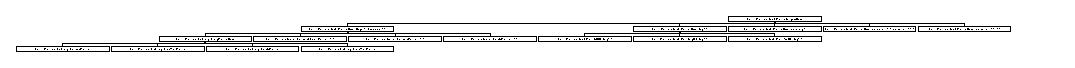
\includegraphics[height=0.471380cm]{class_catch_1_1_matchers_1_1_impl_1_1_matcher_untyped_base}
\end{center}
\end{figure}
\subsection*{Public Member Functions}
\begin{DoxyCompactItemize}
\item 
std\+::string \mbox{\hyperlink{class_catch_1_1_matchers_1_1_impl_1_1_matcher_untyped_base_a5982c7c80ca71dfe2298babadad7a453}{to\+String}} () const
\end{DoxyCompactItemize}
\subsection*{Protected Member Functions}
\begin{DoxyCompactItemize}
\item 
virtual \mbox{\hyperlink{class_catch_1_1_matchers_1_1_impl_1_1_matcher_untyped_base_a853be93ce33f71b5abede38081c79e9d}{$\sim$\+Matcher\+Untyped\+Base}} ()
\item 
virtual std\+::string \mbox{\hyperlink{class_catch_1_1_matchers_1_1_impl_1_1_matcher_untyped_base_a91d3a907dbfcbb596077df24f6e11fe2}{describe}} () const =0
\end{DoxyCompactItemize}
\subsection*{Protected Attributes}
\begin{DoxyCompactItemize}
\item 
std\+::string \mbox{\hyperlink{class_catch_1_1_matchers_1_1_impl_1_1_matcher_untyped_base_a951095c462657e7097a9a6dc4dde813f}{m\+\_\+cached\+To\+String}}
\end{DoxyCompactItemize}


\subsection{Constructor \& Destructor Documentation}
\mbox{\Hypertarget{class_catch_1_1_matchers_1_1_impl_1_1_matcher_untyped_base_a853be93ce33f71b5abede38081c79e9d}\label{class_catch_1_1_matchers_1_1_impl_1_1_matcher_untyped_base_a853be93ce33f71b5abede38081c79e9d}} 
\index{Catch\+::\+Matchers\+::\+Impl\+::\+Matcher\+Untyped\+Base@{Catch\+::\+Matchers\+::\+Impl\+::\+Matcher\+Untyped\+Base}!````~Matcher\+Untyped\+Base@{$\sim$\+Matcher\+Untyped\+Base}}
\index{````~Matcher\+Untyped\+Base@{$\sim$\+Matcher\+Untyped\+Base}!Catch\+::\+Matchers\+::\+Impl\+::\+Matcher\+Untyped\+Base@{Catch\+::\+Matchers\+::\+Impl\+::\+Matcher\+Untyped\+Base}}
\subsubsection{\texorpdfstring{$\sim$\+Matcher\+Untyped\+Base()}{~MatcherUntypedBase()}}
{\footnotesize\ttfamily virtual Catch\+::\+Matchers\+::\+Impl\+::\+Matcher\+Untyped\+Base\+::$\sim$\+Matcher\+Untyped\+Base (\begin{DoxyParamCaption}{ }\end{DoxyParamCaption})\hspace{0.3cm}{\ttfamily [protected]}, {\ttfamily [virtual]}}



\subsection{Member Function Documentation}
\mbox{\Hypertarget{class_catch_1_1_matchers_1_1_impl_1_1_matcher_untyped_base_a91d3a907dbfcbb596077df24f6e11fe2}\label{class_catch_1_1_matchers_1_1_impl_1_1_matcher_untyped_base_a91d3a907dbfcbb596077df24f6e11fe2}} 
\index{Catch\+::\+Matchers\+::\+Impl\+::\+Matcher\+Untyped\+Base@{Catch\+::\+Matchers\+::\+Impl\+::\+Matcher\+Untyped\+Base}!describe@{describe}}
\index{describe@{describe}!Catch\+::\+Matchers\+::\+Impl\+::\+Matcher\+Untyped\+Base@{Catch\+::\+Matchers\+::\+Impl\+::\+Matcher\+Untyped\+Base}}
\subsubsection{\texorpdfstring{describe()}{describe()}}
{\footnotesize\ttfamily virtual std\+::string Catch\+::\+Matchers\+::\+Impl\+::\+Matcher\+Untyped\+Base\+::describe (\begin{DoxyParamCaption}{ }\end{DoxyParamCaption}) const\hspace{0.3cm}{\ttfamily [protected]}, {\ttfamily [pure virtual]}}



Implemented in \mbox{\hyperlink{struct_catch_1_1_matchers_1_1_vector_1_1_equals_matcher_aca79ade26f4a75b2a57005067e086e35}{Catch\+::\+Matchers\+::\+Vector\+::\+Equals\+Matcher$<$ T $>$}}, \mbox{\hyperlink{struct_catch_1_1_matchers_1_1_vector_1_1_contains_matcher_add1a31f049cec89f980424ecdb7027ac}{Catch\+::\+Matchers\+::\+Vector\+::\+Contains\+Matcher$<$ T $>$}}, \mbox{\hyperlink{struct_catch_1_1_matchers_1_1_vector_1_1_contains_element_matcher_a5a869772714dd045816707b74b217664}{Catch\+::\+Matchers\+::\+Vector\+::\+Contains\+Element\+Matcher$<$ T $>$}}, \mbox{\hyperlink{struct_catch_1_1_matchers_1_1_std_string_1_1_string_matcher_base_a9d15cfb882efbea778b2ed29e7f48f37}{Catch\+::\+Matchers\+::\+Std\+String\+::\+String\+Matcher\+Base}}, \mbox{\hyperlink{struct_catch_1_1_matchers_1_1_impl_1_1_match_not_of_a62bdc7dcb9ff000438a4ed3d5483a248}{Catch\+::\+Matchers\+::\+Impl\+::\+Match\+Not\+Of$<$ Arg\+T $>$}}, \mbox{\hyperlink{struct_catch_1_1_matchers_1_1_impl_1_1_match_any_of_a020f5d7889d8cd8be9ad309c690147b6}{Catch\+::\+Matchers\+::\+Impl\+::\+Match\+Any\+Of$<$ Arg\+T $>$}}, and \mbox{\hyperlink{struct_catch_1_1_matchers_1_1_impl_1_1_match_all_of_aaefeba99a0b35425203468a65bff544b}{Catch\+::\+Matchers\+::\+Impl\+::\+Match\+All\+Of$<$ Arg\+T $>$}}.

\mbox{\Hypertarget{class_catch_1_1_matchers_1_1_impl_1_1_matcher_untyped_base_a5982c7c80ca71dfe2298babadad7a453}\label{class_catch_1_1_matchers_1_1_impl_1_1_matcher_untyped_base_a5982c7c80ca71dfe2298babadad7a453}} 
\index{Catch\+::\+Matchers\+::\+Impl\+::\+Matcher\+Untyped\+Base@{Catch\+::\+Matchers\+::\+Impl\+::\+Matcher\+Untyped\+Base}!to\+String@{to\+String}}
\index{to\+String@{to\+String}!Catch\+::\+Matchers\+::\+Impl\+::\+Matcher\+Untyped\+Base@{Catch\+::\+Matchers\+::\+Impl\+::\+Matcher\+Untyped\+Base}}
\subsubsection{\texorpdfstring{to\+String()}{toString()}}
{\footnotesize\ttfamily std\+::string Catch\+::\+Matchers\+::\+Impl\+::\+Matcher\+Untyped\+Base\+::to\+String (\begin{DoxyParamCaption}{ }\end{DoxyParamCaption}) const\hspace{0.3cm}{\ttfamily [inline]}}



\subsection{Member Data Documentation}
\mbox{\Hypertarget{class_catch_1_1_matchers_1_1_impl_1_1_matcher_untyped_base_a951095c462657e7097a9a6dc4dde813f}\label{class_catch_1_1_matchers_1_1_impl_1_1_matcher_untyped_base_a951095c462657e7097a9a6dc4dde813f}} 
\index{Catch\+::\+Matchers\+::\+Impl\+::\+Matcher\+Untyped\+Base@{Catch\+::\+Matchers\+::\+Impl\+::\+Matcher\+Untyped\+Base}!m\+\_\+cached\+To\+String@{m\+\_\+cached\+To\+String}}
\index{m\+\_\+cached\+To\+String@{m\+\_\+cached\+To\+String}!Catch\+::\+Matchers\+::\+Impl\+::\+Matcher\+Untyped\+Base@{Catch\+::\+Matchers\+::\+Impl\+::\+Matcher\+Untyped\+Base}}
\subsubsection{\texorpdfstring{m\+\_\+cached\+To\+String}{m\_cachedToString}}
{\footnotesize\ttfamily std\+::string Catch\+::\+Matchers\+::\+Impl\+::\+Matcher\+Untyped\+Base\+::m\+\_\+cached\+To\+String\hspace{0.3cm}{\ttfamily [mutable]}, {\ttfamily [protected]}}



The documentation for this class was generated from the following file\+:\begin{DoxyCompactItemize}
\item 
include/\mbox{\hyperlink{catch_8hpp}{catch.\+hpp}}\end{DoxyCompactItemize}

\hypertarget{class_catch_1_1_match_expression}{}\section{Catch\+:\+:Match\+Expression$<$ ArgT, MatcherT $>$ Class Template Reference}
\label{class_catch_1_1_match_expression}\index{Catch\+::\+Match\+Expression$<$ Arg\+T, Matcher\+T $>$@{Catch\+::\+Match\+Expression$<$ Arg\+T, Matcher\+T $>$}}


{\ttfamily \#include $<$catch.\+hpp$>$}

Inheritance diagram for Catch\+:\+:Match\+Expression$<$ ArgT, MatcherT $>$\+:\begin{figure}[H]
\begin{center}
\leavevmode
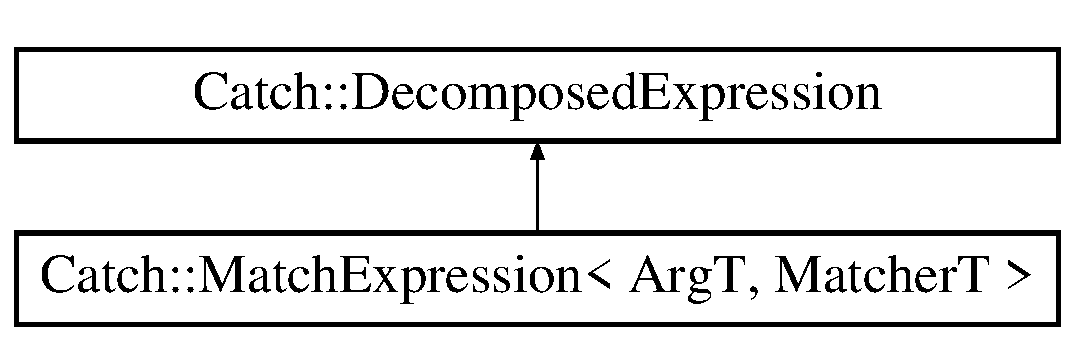
\includegraphics[height=2.000000cm]{class_catch_1_1_match_expression}
\end{center}
\end{figure}
\subsection*{Public Member Functions}
\begin{DoxyCompactItemize}
\item 
\mbox{\hyperlink{class_catch_1_1_match_expression_a506f25bad7970cb35f9dbe54763a8ca5}{Match\+Expression}} (ArgT arg, MatcherT matcher, char const $\ast$matcher\+String)
\item 
virtual bool \mbox{\hyperlink{class_catch_1_1_match_expression_ac4edf6e9a6e5762a487db1486d0d1f45}{is\+Binary\+Expression}} () const \mbox{\hyperlink{catch_8hpp_a8ecdce4d3f57835f707915ae831eb847}{C\+A\+T\+C\+H\+\_\+\+O\+V\+E\+R\+R\+I\+DE}}
\item 
virtual void \mbox{\hyperlink{class_catch_1_1_match_expression_a4410a93bc5b8241eb2502f400fce7ec4}{reconstruct\+Expression}} (std\+::string \&dest) const \mbox{\hyperlink{catch_8hpp_a8ecdce4d3f57835f707915ae831eb847}{C\+A\+T\+C\+H\+\_\+\+O\+V\+E\+R\+R\+I\+DE}}
\end{DoxyCompactItemize}


\subsection{Constructor \& Destructor Documentation}
\mbox{\Hypertarget{class_catch_1_1_match_expression_a506f25bad7970cb35f9dbe54763a8ca5}\label{class_catch_1_1_match_expression_a506f25bad7970cb35f9dbe54763a8ca5}} 
\index{Catch\+::\+Match\+Expression@{Catch\+::\+Match\+Expression}!Match\+Expression@{Match\+Expression}}
\index{Match\+Expression@{Match\+Expression}!Catch\+::\+Match\+Expression@{Catch\+::\+Match\+Expression}}
\subsubsection{\texorpdfstring{Match\+Expression()}{MatchExpression()}}
{\footnotesize\ttfamily template$<$typename ArgT , typename MatcherT $>$ \\
\mbox{\hyperlink{class_catch_1_1_match_expression}{Catch\+::\+Match\+Expression}}$<$ ArgT, MatcherT $>$\+::\mbox{\hyperlink{class_catch_1_1_match_expression}{Match\+Expression}} (\begin{DoxyParamCaption}\item[{ArgT}]{arg,  }\item[{MatcherT}]{matcher,  }\item[{char const $\ast$}]{matcher\+String }\end{DoxyParamCaption})\hspace{0.3cm}{\ttfamily [inline]}}



\subsection{Member Function Documentation}
\mbox{\Hypertarget{class_catch_1_1_match_expression_ac4edf6e9a6e5762a487db1486d0d1f45}\label{class_catch_1_1_match_expression_ac4edf6e9a6e5762a487db1486d0d1f45}} 
\index{Catch\+::\+Match\+Expression@{Catch\+::\+Match\+Expression}!is\+Binary\+Expression@{is\+Binary\+Expression}}
\index{is\+Binary\+Expression@{is\+Binary\+Expression}!Catch\+::\+Match\+Expression@{Catch\+::\+Match\+Expression}}
\subsubsection{\texorpdfstring{is\+Binary\+Expression()}{isBinaryExpression()}}
{\footnotesize\ttfamily template$<$typename ArgT , typename MatcherT $>$ \\
virtual bool \mbox{\hyperlink{class_catch_1_1_match_expression}{Catch\+::\+Match\+Expression}}$<$ ArgT, MatcherT $>$\+::is\+Binary\+Expression (\begin{DoxyParamCaption}{ }\end{DoxyParamCaption}) const\hspace{0.3cm}{\ttfamily [inline]}, {\ttfamily [virtual]}}



Reimplemented from \mbox{\hyperlink{struct_catch_1_1_decomposed_expression_a1c458ece47b71f093290dbdf9bb31fdb}{Catch\+::\+Decomposed\+Expression}}.

\mbox{\Hypertarget{class_catch_1_1_match_expression_a4410a93bc5b8241eb2502f400fce7ec4}\label{class_catch_1_1_match_expression_a4410a93bc5b8241eb2502f400fce7ec4}} 
\index{Catch\+::\+Match\+Expression@{Catch\+::\+Match\+Expression}!reconstruct\+Expression@{reconstruct\+Expression}}
\index{reconstruct\+Expression@{reconstruct\+Expression}!Catch\+::\+Match\+Expression@{Catch\+::\+Match\+Expression}}
\subsubsection{\texorpdfstring{reconstruct\+Expression()}{reconstructExpression()}}
{\footnotesize\ttfamily template$<$typename ArgT , typename MatcherT $>$ \\
virtual void \mbox{\hyperlink{class_catch_1_1_match_expression}{Catch\+::\+Match\+Expression}}$<$ ArgT, MatcherT $>$\+::reconstruct\+Expression (\begin{DoxyParamCaption}\item[{std\+::string \&}]{dest }\end{DoxyParamCaption}) const\hspace{0.3cm}{\ttfamily [inline]}, {\ttfamily [virtual]}}



Implements \mbox{\hyperlink{struct_catch_1_1_decomposed_expression_a9ce7f356dc96f11f80e40c82f5aa7e55}{Catch\+::\+Decomposed\+Expression}}.



The documentation for this class was generated from the following file\+:\begin{DoxyCompactItemize}
\item 
include/\mbox{\hyperlink{catch_8hpp}{catch.\+hpp}}\end{DoxyCompactItemize}

\hypertarget{struct_catch_1_1_matchers_1_1_impl_1_1_match_not_of}{}\section{Catch\+:\+:Matchers\+:\+:Impl\+:\+:Match\+Not\+Of$<$ ArgT $>$ Struct Template Reference}
\label{struct_catch_1_1_matchers_1_1_impl_1_1_match_not_of}\index{Catch\+::\+Matchers\+::\+Impl\+::\+Match\+Not\+Of$<$ Arg\+T $>$@{Catch\+::\+Matchers\+::\+Impl\+::\+Match\+Not\+Of$<$ Arg\+T $>$}}


{\ttfamily \#include $<$catch.\+hpp$>$}

Inheritance diagram for Catch\+:\+:Matchers\+:\+:Impl\+:\+:Match\+Not\+Of$<$ ArgT $>$\+:\begin{figure}[H]
\begin{center}
\leavevmode
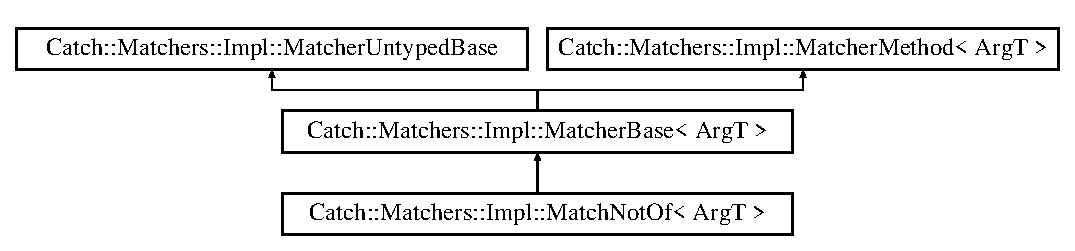
\includegraphics[height=2.926829cm]{struct_catch_1_1_matchers_1_1_impl_1_1_match_not_of}
\end{center}
\end{figure}
\subsection*{Public Member Functions}
\begin{DoxyCompactItemize}
\item 
\mbox{\hyperlink{struct_catch_1_1_matchers_1_1_impl_1_1_match_not_of_a47afdd9e4c3354cef85adc3186097ae4}{Match\+Not\+Of}} (\mbox{\hyperlink{struct_catch_1_1_matchers_1_1_impl_1_1_matcher_base}{Matcher\+Base}}$<$ ArgT $>$ const \&underlying\+Matcher)
\item 
virtual bool \mbox{\hyperlink{struct_catch_1_1_matchers_1_1_impl_1_1_match_not_of_a1b9ad6566e4ab0f292d2903f557307cc}{match}} (ArgT const \&arg) const \mbox{\hyperlink{catch_8hpp_a8ecdce4d3f57835f707915ae831eb847}{C\+A\+T\+C\+H\+\_\+\+O\+V\+E\+R\+R\+I\+DE}}
\item 
virtual std\+::string \mbox{\hyperlink{struct_catch_1_1_matchers_1_1_impl_1_1_match_not_of_a62bdc7dcb9ff000438a4ed3d5483a248}{describe}} () const \mbox{\hyperlink{catch_8hpp_a8ecdce4d3f57835f707915ae831eb847}{C\+A\+T\+C\+H\+\_\+\+O\+V\+E\+R\+R\+I\+DE}}
\end{DoxyCompactItemize}
\subsection*{Public Attributes}
\begin{DoxyCompactItemize}
\item 
\mbox{\hyperlink{struct_catch_1_1_matchers_1_1_impl_1_1_matcher_base}{Matcher\+Base}}$<$ ArgT $>$ const  \& \mbox{\hyperlink{struct_catch_1_1_matchers_1_1_impl_1_1_match_not_of_af7ac67f112b0e93796b048a47329aad4}{m\+\_\+underlying\+Matcher}}
\end{DoxyCompactItemize}
\subsection*{Additional Inherited Members}


\subsection{Constructor \& Destructor Documentation}
\mbox{\Hypertarget{struct_catch_1_1_matchers_1_1_impl_1_1_match_not_of_a47afdd9e4c3354cef85adc3186097ae4}\label{struct_catch_1_1_matchers_1_1_impl_1_1_match_not_of_a47afdd9e4c3354cef85adc3186097ae4}} 
\index{Catch\+::\+Matchers\+::\+Impl\+::\+Match\+Not\+Of@{Catch\+::\+Matchers\+::\+Impl\+::\+Match\+Not\+Of}!Match\+Not\+Of@{Match\+Not\+Of}}
\index{Match\+Not\+Of@{Match\+Not\+Of}!Catch\+::\+Matchers\+::\+Impl\+::\+Match\+Not\+Of@{Catch\+::\+Matchers\+::\+Impl\+::\+Match\+Not\+Of}}
\subsubsection{\texorpdfstring{Match\+Not\+Of()}{MatchNotOf()}}
{\footnotesize\ttfamily template$<$typename ArgT$>$ \\
\mbox{\hyperlink{struct_catch_1_1_matchers_1_1_impl_1_1_match_not_of}{Catch\+::\+Matchers\+::\+Impl\+::\+Match\+Not\+Of}}$<$ ArgT $>$\+::\mbox{\hyperlink{struct_catch_1_1_matchers_1_1_impl_1_1_match_not_of}{Match\+Not\+Of}} (\begin{DoxyParamCaption}\item[{\mbox{\hyperlink{struct_catch_1_1_matchers_1_1_impl_1_1_matcher_base}{Matcher\+Base}}$<$ ArgT $>$ const \&}]{underlying\+Matcher }\end{DoxyParamCaption})\hspace{0.3cm}{\ttfamily [inline]}}



\subsection{Member Function Documentation}
\mbox{\Hypertarget{struct_catch_1_1_matchers_1_1_impl_1_1_match_not_of_a62bdc7dcb9ff000438a4ed3d5483a248}\label{struct_catch_1_1_matchers_1_1_impl_1_1_match_not_of_a62bdc7dcb9ff000438a4ed3d5483a248}} 
\index{Catch\+::\+Matchers\+::\+Impl\+::\+Match\+Not\+Of@{Catch\+::\+Matchers\+::\+Impl\+::\+Match\+Not\+Of}!describe@{describe}}
\index{describe@{describe}!Catch\+::\+Matchers\+::\+Impl\+::\+Match\+Not\+Of@{Catch\+::\+Matchers\+::\+Impl\+::\+Match\+Not\+Of}}
\subsubsection{\texorpdfstring{describe()}{describe()}}
{\footnotesize\ttfamily template$<$typename ArgT$>$ \\
virtual std\+::string \mbox{\hyperlink{struct_catch_1_1_matchers_1_1_impl_1_1_match_not_of}{Catch\+::\+Matchers\+::\+Impl\+::\+Match\+Not\+Of}}$<$ ArgT $>$\+::describe (\begin{DoxyParamCaption}{ }\end{DoxyParamCaption}) const\hspace{0.3cm}{\ttfamily [inline]}, {\ttfamily [virtual]}}



Implements \mbox{\hyperlink{class_catch_1_1_matchers_1_1_impl_1_1_matcher_untyped_base_a91d3a907dbfcbb596077df24f6e11fe2}{Catch\+::\+Matchers\+::\+Impl\+::\+Matcher\+Untyped\+Base}}.

\mbox{\Hypertarget{struct_catch_1_1_matchers_1_1_impl_1_1_match_not_of_a1b9ad6566e4ab0f292d2903f557307cc}\label{struct_catch_1_1_matchers_1_1_impl_1_1_match_not_of_a1b9ad6566e4ab0f292d2903f557307cc}} 
\index{Catch\+::\+Matchers\+::\+Impl\+::\+Match\+Not\+Of@{Catch\+::\+Matchers\+::\+Impl\+::\+Match\+Not\+Of}!match@{match}}
\index{match@{match}!Catch\+::\+Matchers\+::\+Impl\+::\+Match\+Not\+Of@{Catch\+::\+Matchers\+::\+Impl\+::\+Match\+Not\+Of}}
\subsubsection{\texorpdfstring{match()}{match()}}
{\footnotesize\ttfamily template$<$typename ArgT$>$ \\
virtual bool \mbox{\hyperlink{struct_catch_1_1_matchers_1_1_impl_1_1_match_not_of}{Catch\+::\+Matchers\+::\+Impl\+::\+Match\+Not\+Of}}$<$ ArgT $>$\+::match (\begin{DoxyParamCaption}\item[{ArgT const \&}]{arg }\end{DoxyParamCaption}) const\hspace{0.3cm}{\ttfamily [inline]}, {\ttfamily [virtual]}}



Implements \mbox{\hyperlink{struct_catch_1_1_matchers_1_1_impl_1_1_matcher_method_ae0920ff9e817acf08e1bb0cbcb044e30}{Catch\+::\+Matchers\+::\+Impl\+::\+Matcher\+Method$<$ Arg\+T $>$}}.



\subsection{Member Data Documentation}
\mbox{\Hypertarget{struct_catch_1_1_matchers_1_1_impl_1_1_match_not_of_af7ac67f112b0e93796b048a47329aad4}\label{struct_catch_1_1_matchers_1_1_impl_1_1_match_not_of_af7ac67f112b0e93796b048a47329aad4}} 
\index{Catch\+::\+Matchers\+::\+Impl\+::\+Match\+Not\+Of@{Catch\+::\+Matchers\+::\+Impl\+::\+Match\+Not\+Of}!m\+\_\+underlying\+Matcher@{m\+\_\+underlying\+Matcher}}
\index{m\+\_\+underlying\+Matcher@{m\+\_\+underlying\+Matcher}!Catch\+::\+Matchers\+::\+Impl\+::\+Match\+Not\+Of@{Catch\+::\+Matchers\+::\+Impl\+::\+Match\+Not\+Of}}
\subsubsection{\texorpdfstring{m\+\_\+underlying\+Matcher}{m\_underlyingMatcher}}
{\footnotesize\ttfamily template$<$typename ArgT$>$ \\
\mbox{\hyperlink{struct_catch_1_1_matchers_1_1_impl_1_1_matcher_base}{Matcher\+Base}}$<$ArgT$>$ const\& \mbox{\hyperlink{struct_catch_1_1_matchers_1_1_impl_1_1_match_not_of}{Catch\+::\+Matchers\+::\+Impl\+::\+Match\+Not\+Of}}$<$ ArgT $>$\+::m\+\_\+underlying\+Matcher}



The documentation for this struct was generated from the following file\+:\begin{DoxyCompactItemize}
\item 
include/\mbox{\hyperlink{catch_8hpp}{catch.\+hpp}}\end{DoxyCompactItemize}

\hypertarget{struct_catch_1_1_message_builder}{}\section{Catch\+:\+:Message\+Builder Struct Reference}
\label{struct_catch_1_1_message_builder}\index{Catch\+::\+Message\+Builder@{Catch\+::\+Message\+Builder}}


{\ttfamily \#include $<$catch.\+hpp$>$}

\subsection*{Public Member Functions}
\begin{DoxyCompactItemize}
\item 
\mbox{\hyperlink{struct_catch_1_1_message_builder_ab0c6378e722680bf58852c6ee2b6e724}{Message\+Builder}} (std\+::string const \&macro\+Name, \mbox{\hyperlink{struct_catch_1_1_source_line_info}{Source\+Line\+Info}} const \&line\+Info, \mbox{\hyperlink{struct_catch_1_1_result_was_a624e1ee3661fcf6094ceef1f654601ef}{Result\+Was\+::\+Of\+Type}} type)
\item 
{\footnotesize template$<$typename T $>$ }\\\mbox{\hyperlink{struct_catch_1_1_message_builder}{Message\+Builder}} \& \mbox{\hyperlink{struct_catch_1_1_message_builder_a20fa48d069b20dddcc2d3df8abb123c1}{operator$<$$<$}} (T const \&value)
\end{DoxyCompactItemize}
\subsection*{Public Attributes}
\begin{DoxyCompactItemize}
\item 
\mbox{\hyperlink{struct_catch_1_1_message_info}{Message\+Info}} \mbox{\hyperlink{struct_catch_1_1_message_builder_a979f1c2b36d78f80ee275bfa5ba0209f}{m\+\_\+info}}
\item 
std\+::ostringstream \mbox{\hyperlink{struct_catch_1_1_message_builder_a6488ab0cc4ea52affc9c0612c7c5df6b}{m\+\_\+stream}}
\end{DoxyCompactItemize}


\subsection{Constructor \& Destructor Documentation}
\mbox{\Hypertarget{struct_catch_1_1_message_builder_ab0c6378e722680bf58852c6ee2b6e724}\label{struct_catch_1_1_message_builder_ab0c6378e722680bf58852c6ee2b6e724}} 
\index{Catch\+::\+Message\+Builder@{Catch\+::\+Message\+Builder}!Message\+Builder@{Message\+Builder}}
\index{Message\+Builder@{Message\+Builder}!Catch\+::\+Message\+Builder@{Catch\+::\+Message\+Builder}}
\subsubsection{\texorpdfstring{Message\+Builder()}{MessageBuilder()}}
{\footnotesize\ttfamily Catch\+::\+Message\+Builder\+::\+Message\+Builder (\begin{DoxyParamCaption}\item[{std\+::string const \&}]{macro\+Name,  }\item[{\mbox{\hyperlink{struct_catch_1_1_source_line_info}{Source\+Line\+Info}} const \&}]{line\+Info,  }\item[{\mbox{\hyperlink{struct_catch_1_1_result_was_a624e1ee3661fcf6094ceef1f654601ef}{Result\+Was\+::\+Of\+Type}}}]{type }\end{DoxyParamCaption})\hspace{0.3cm}{\ttfamily [inline]}}



\subsection{Member Function Documentation}
\mbox{\Hypertarget{struct_catch_1_1_message_builder_a20fa48d069b20dddcc2d3df8abb123c1}\label{struct_catch_1_1_message_builder_a20fa48d069b20dddcc2d3df8abb123c1}} 
\index{Catch\+::\+Message\+Builder@{Catch\+::\+Message\+Builder}!operator$<$$<$@{operator$<$$<$}}
\index{operator$<$$<$@{operator$<$$<$}!Catch\+::\+Message\+Builder@{Catch\+::\+Message\+Builder}}
\subsubsection{\texorpdfstring{operator$<$$<$()}{operator<<()}}
{\footnotesize\ttfamily template$<$typename T $>$ \\
\mbox{\hyperlink{struct_catch_1_1_message_builder}{Message\+Builder}}\& Catch\+::\+Message\+Builder\+::operator$<$$<$ (\begin{DoxyParamCaption}\item[{T const \&}]{value }\end{DoxyParamCaption})\hspace{0.3cm}{\ttfamily [inline]}}



\subsection{Member Data Documentation}
\mbox{\Hypertarget{struct_catch_1_1_message_builder_a979f1c2b36d78f80ee275bfa5ba0209f}\label{struct_catch_1_1_message_builder_a979f1c2b36d78f80ee275bfa5ba0209f}} 
\index{Catch\+::\+Message\+Builder@{Catch\+::\+Message\+Builder}!m\+\_\+info@{m\+\_\+info}}
\index{m\+\_\+info@{m\+\_\+info}!Catch\+::\+Message\+Builder@{Catch\+::\+Message\+Builder}}
\subsubsection{\texorpdfstring{m\+\_\+info}{m\_info}}
{\footnotesize\ttfamily \mbox{\hyperlink{struct_catch_1_1_message_info}{Message\+Info}} Catch\+::\+Message\+Builder\+::m\+\_\+info}

\mbox{\Hypertarget{struct_catch_1_1_message_builder_a6488ab0cc4ea52affc9c0612c7c5df6b}\label{struct_catch_1_1_message_builder_a6488ab0cc4ea52affc9c0612c7c5df6b}} 
\index{Catch\+::\+Message\+Builder@{Catch\+::\+Message\+Builder}!m\+\_\+stream@{m\+\_\+stream}}
\index{m\+\_\+stream@{m\+\_\+stream}!Catch\+::\+Message\+Builder@{Catch\+::\+Message\+Builder}}
\subsubsection{\texorpdfstring{m\+\_\+stream}{m\_stream}}
{\footnotesize\ttfamily std\+::ostringstream Catch\+::\+Message\+Builder\+::m\+\_\+stream}



The documentation for this struct was generated from the following file\+:\begin{DoxyCompactItemize}
\item 
include/\mbox{\hyperlink{catch_8hpp}{catch.\+hpp}}\end{DoxyCompactItemize}

\hypertarget{struct_catch_1_1_message_info}{}\section{Catch\+:\+:Message\+Info Struct Reference}
\label{struct_catch_1_1_message_info}\index{Catch\+::\+Message\+Info@{Catch\+::\+Message\+Info}}


{\ttfamily \#include $<$catch.\+hpp$>$}

\subsection*{Public Member Functions}
\begin{DoxyCompactItemize}
\item 
\mbox{\hyperlink{struct_catch_1_1_message_info_a2e336c33ebef7af3c1bbae6a56e14f8a}{Message\+Info}} (std\+::string const \&\+\_\+macro\+Name, \mbox{\hyperlink{struct_catch_1_1_source_line_info}{Source\+Line\+Info}} const \&\+\_\+line\+Info, \mbox{\hyperlink{struct_catch_1_1_result_was_a624e1ee3661fcf6094ceef1f654601ef}{Result\+Was\+::\+Of\+Type}} \+\_\+type)
\item 
bool \mbox{\hyperlink{struct_catch_1_1_message_info_af4b37f2172ba55395813b4bb6bbbde1a}{operator==}} (\mbox{\hyperlink{struct_catch_1_1_message_info}{Message\+Info}} const \&other) const
\item 
bool \mbox{\hyperlink{struct_catch_1_1_message_info_a8254cb8fca2da02a29a9843cdcb79df1}{operator$<$}} (\mbox{\hyperlink{struct_catch_1_1_message_info}{Message\+Info}} const \&other) const
\end{DoxyCompactItemize}
\subsection*{Public Attributes}
\begin{DoxyCompactItemize}
\item 
std\+::string \mbox{\hyperlink{struct_catch_1_1_message_info_a156ade4b3cc731f6ec7b542ae47ba8e3}{macro\+Name}}
\item 
\mbox{\hyperlink{struct_catch_1_1_source_line_info}{Source\+Line\+Info}} \mbox{\hyperlink{struct_catch_1_1_message_info_a985165328723e599696ebd8e43195cc5}{line\+Info}}
\item 
\mbox{\hyperlink{struct_catch_1_1_result_was_a624e1ee3661fcf6094ceef1f654601ef}{Result\+Was\+::\+Of\+Type}} \mbox{\hyperlink{struct_catch_1_1_message_info_ae928b9117465c696e45951d9d0284e78}{type}}
\item 
std\+::string \mbox{\hyperlink{struct_catch_1_1_message_info_ab6cd06e050bf426c6577502a5c50e256}{message}}
\item 
unsigned int \mbox{\hyperlink{struct_catch_1_1_message_info_a7f4f57ea21e50160adefce7b68a781d6}{sequence}}
\end{DoxyCompactItemize}


\subsection{Constructor \& Destructor Documentation}
\mbox{\Hypertarget{struct_catch_1_1_message_info_a2e336c33ebef7af3c1bbae6a56e14f8a}\label{struct_catch_1_1_message_info_a2e336c33ebef7af3c1bbae6a56e14f8a}} 
\index{Catch\+::\+Message\+Info@{Catch\+::\+Message\+Info}!Message\+Info@{Message\+Info}}
\index{Message\+Info@{Message\+Info}!Catch\+::\+Message\+Info@{Catch\+::\+Message\+Info}}
\subsubsection{\texorpdfstring{Message\+Info()}{MessageInfo()}}
{\footnotesize\ttfamily Catch\+::\+Message\+Info\+::\+Message\+Info (\begin{DoxyParamCaption}\item[{std\+::string const \&}]{\+\_\+macro\+Name,  }\item[{\mbox{\hyperlink{struct_catch_1_1_source_line_info}{Source\+Line\+Info}} const \&}]{\+\_\+line\+Info,  }\item[{\mbox{\hyperlink{struct_catch_1_1_result_was_a624e1ee3661fcf6094ceef1f654601ef}{Result\+Was\+::\+Of\+Type}}}]{\+\_\+type }\end{DoxyParamCaption})}



\subsection{Member Function Documentation}
\mbox{\Hypertarget{struct_catch_1_1_message_info_a8254cb8fca2da02a29a9843cdcb79df1}\label{struct_catch_1_1_message_info_a8254cb8fca2da02a29a9843cdcb79df1}} 
\index{Catch\+::\+Message\+Info@{Catch\+::\+Message\+Info}!operator$<$@{operator$<$}}
\index{operator$<$@{operator$<$}!Catch\+::\+Message\+Info@{Catch\+::\+Message\+Info}}
\subsubsection{\texorpdfstring{operator$<$()}{operator<()}}
{\footnotesize\ttfamily bool Catch\+::\+Message\+Info\+::operator$<$ (\begin{DoxyParamCaption}\item[{\mbox{\hyperlink{struct_catch_1_1_message_info}{Message\+Info}} const \&}]{other }\end{DoxyParamCaption}) const\hspace{0.3cm}{\ttfamily [inline]}}

\mbox{\Hypertarget{struct_catch_1_1_message_info_af4b37f2172ba55395813b4bb6bbbde1a}\label{struct_catch_1_1_message_info_af4b37f2172ba55395813b4bb6bbbde1a}} 
\index{Catch\+::\+Message\+Info@{Catch\+::\+Message\+Info}!operator==@{operator==}}
\index{operator==@{operator==}!Catch\+::\+Message\+Info@{Catch\+::\+Message\+Info}}
\subsubsection{\texorpdfstring{operator==()}{operator==()}}
{\footnotesize\ttfamily bool Catch\+::\+Message\+Info\+::operator== (\begin{DoxyParamCaption}\item[{\mbox{\hyperlink{struct_catch_1_1_message_info}{Message\+Info}} const \&}]{other }\end{DoxyParamCaption}) const\hspace{0.3cm}{\ttfamily [inline]}}



\subsection{Member Data Documentation}
\mbox{\Hypertarget{struct_catch_1_1_message_info_a985165328723e599696ebd8e43195cc5}\label{struct_catch_1_1_message_info_a985165328723e599696ebd8e43195cc5}} 
\index{Catch\+::\+Message\+Info@{Catch\+::\+Message\+Info}!line\+Info@{line\+Info}}
\index{line\+Info@{line\+Info}!Catch\+::\+Message\+Info@{Catch\+::\+Message\+Info}}
\subsubsection{\texorpdfstring{line\+Info}{lineInfo}}
{\footnotesize\ttfamily \mbox{\hyperlink{struct_catch_1_1_source_line_info}{Source\+Line\+Info}} Catch\+::\+Message\+Info\+::line\+Info}

\mbox{\Hypertarget{struct_catch_1_1_message_info_a156ade4b3cc731f6ec7b542ae47ba8e3}\label{struct_catch_1_1_message_info_a156ade4b3cc731f6ec7b542ae47ba8e3}} 
\index{Catch\+::\+Message\+Info@{Catch\+::\+Message\+Info}!macro\+Name@{macro\+Name}}
\index{macro\+Name@{macro\+Name}!Catch\+::\+Message\+Info@{Catch\+::\+Message\+Info}}
\subsubsection{\texorpdfstring{macro\+Name}{macroName}}
{\footnotesize\ttfamily std\+::string Catch\+::\+Message\+Info\+::macro\+Name}

\mbox{\Hypertarget{struct_catch_1_1_message_info_ab6cd06e050bf426c6577502a5c50e256}\label{struct_catch_1_1_message_info_ab6cd06e050bf426c6577502a5c50e256}} 
\index{Catch\+::\+Message\+Info@{Catch\+::\+Message\+Info}!message@{message}}
\index{message@{message}!Catch\+::\+Message\+Info@{Catch\+::\+Message\+Info}}
\subsubsection{\texorpdfstring{message}{message}}
{\footnotesize\ttfamily std\+::string Catch\+::\+Message\+Info\+::message}

\mbox{\Hypertarget{struct_catch_1_1_message_info_a7f4f57ea21e50160adefce7b68a781d6}\label{struct_catch_1_1_message_info_a7f4f57ea21e50160adefce7b68a781d6}} 
\index{Catch\+::\+Message\+Info@{Catch\+::\+Message\+Info}!sequence@{sequence}}
\index{sequence@{sequence}!Catch\+::\+Message\+Info@{Catch\+::\+Message\+Info}}
\subsubsection{\texorpdfstring{sequence}{sequence}}
{\footnotesize\ttfamily unsigned int Catch\+::\+Message\+Info\+::sequence}

\mbox{\Hypertarget{struct_catch_1_1_message_info_ae928b9117465c696e45951d9d0284e78}\label{struct_catch_1_1_message_info_ae928b9117465c696e45951d9d0284e78}} 
\index{Catch\+::\+Message\+Info@{Catch\+::\+Message\+Info}!type@{type}}
\index{type@{type}!Catch\+::\+Message\+Info@{Catch\+::\+Message\+Info}}
\subsubsection{\texorpdfstring{type}{type}}
{\footnotesize\ttfamily \mbox{\hyperlink{struct_catch_1_1_result_was_a624e1ee3661fcf6094ceef1f654601ef}{Result\+Was\+::\+Of\+Type}} Catch\+::\+Message\+Info\+::type}



The documentation for this struct was generated from the following file\+:\begin{DoxyCompactItemize}
\item 
include/\mbox{\hyperlink{catch_8hpp}{catch.\+hpp}}\end{DoxyCompactItemize}

\hypertarget{class_catch_1_1_method_test_case}{}\section{Catch\+:\+:Method\+Test\+Case$<$ C $>$ Class Template Reference}
\label{class_catch_1_1_method_test_case}\index{Catch\+::\+Method\+Test\+Case$<$ C $>$@{Catch\+::\+Method\+Test\+Case$<$ C $>$}}


{\ttfamily \#include $<$catch.\+hpp$>$}

Inheritance diagram for Catch\+:\+:Method\+Test\+Case$<$ C $>$\+:\begin{figure}[H]
\begin{center}
\leavevmode
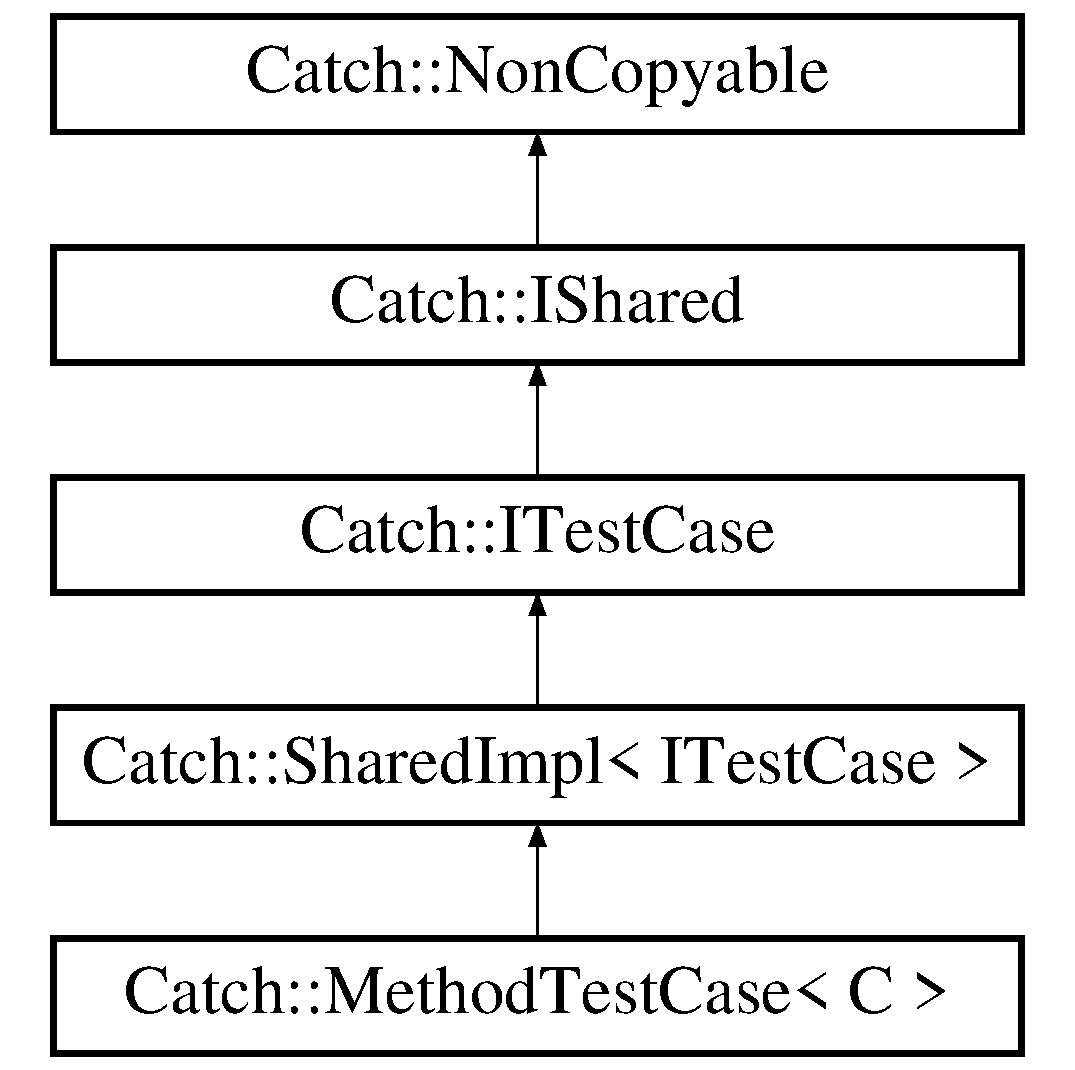
\includegraphics[height=5.000000cm]{class_catch_1_1_method_test_case}
\end{center}
\end{figure}
\subsection*{Public Member Functions}
\begin{DoxyCompactItemize}
\item 
\mbox{\hyperlink{class_catch_1_1_method_test_case_a7b043b85dae371358255dd9dc6582e7b}{Method\+Test\+Case}} (void(C\+::$\ast$method)())
\item 
virtual void \mbox{\hyperlink{class_catch_1_1_method_test_case_a4e2263cfa0646f2980768328cb372793}{invoke}} () const
\end{DoxyCompactItemize}
\subsection*{Additional Inherited Members}


\subsection{Constructor \& Destructor Documentation}
\mbox{\Hypertarget{class_catch_1_1_method_test_case_a7b043b85dae371358255dd9dc6582e7b}\label{class_catch_1_1_method_test_case_a7b043b85dae371358255dd9dc6582e7b}} 
\index{Catch\+::\+Method\+Test\+Case@{Catch\+::\+Method\+Test\+Case}!Method\+Test\+Case@{Method\+Test\+Case}}
\index{Method\+Test\+Case@{Method\+Test\+Case}!Catch\+::\+Method\+Test\+Case@{Catch\+::\+Method\+Test\+Case}}
\subsubsection{\texorpdfstring{Method\+Test\+Case()}{MethodTestCase()}}
{\footnotesize\ttfamily template$<$typename C $>$ \\
\mbox{\hyperlink{class_catch_1_1_method_test_case}{Catch\+::\+Method\+Test\+Case}}$<$ C $>$\+::\mbox{\hyperlink{class_catch_1_1_method_test_case}{Method\+Test\+Case}} (\begin{DoxyParamCaption}\item[{void(C\+::$\ast$)()}]{method }\end{DoxyParamCaption})\hspace{0.3cm}{\ttfamily [inline]}}



\subsection{Member Function Documentation}
\mbox{\Hypertarget{class_catch_1_1_method_test_case_a4e2263cfa0646f2980768328cb372793}\label{class_catch_1_1_method_test_case_a4e2263cfa0646f2980768328cb372793}} 
\index{Catch\+::\+Method\+Test\+Case@{Catch\+::\+Method\+Test\+Case}!invoke@{invoke}}
\index{invoke@{invoke}!Catch\+::\+Method\+Test\+Case@{Catch\+::\+Method\+Test\+Case}}
\subsubsection{\texorpdfstring{invoke()}{invoke()}}
{\footnotesize\ttfamily template$<$typename C $>$ \\
virtual void \mbox{\hyperlink{class_catch_1_1_method_test_case}{Catch\+::\+Method\+Test\+Case}}$<$ C $>$\+::invoke (\begin{DoxyParamCaption}{ }\end{DoxyParamCaption}) const\hspace{0.3cm}{\ttfamily [inline]}, {\ttfamily [virtual]}}



Implements \mbox{\hyperlink{struct_catch_1_1_i_test_case_a678825e62e7c17297621cfeb65588c34}{Catch\+::\+I\+Test\+Case}}.



The documentation for this class was generated from the following file\+:\begin{DoxyCompactItemize}
\item 
include/\mbox{\hyperlink{catch_8hpp}{catch.\+hpp}}\end{DoxyCompactItemize}

\hypertarget{struct_catch_1_1_name_and_desc}{}\section{Catch\+:\+:Name\+And\+Desc Struct Reference}
\label{struct_catch_1_1_name_and_desc}\index{Catch\+::\+Name\+And\+Desc@{Catch\+::\+Name\+And\+Desc}}


{\ttfamily \#include $<$catch.\+hpp$>$}

\subsection*{Public Member Functions}
\begin{DoxyCompactItemize}
\item 
\mbox{\hyperlink{struct_catch_1_1_name_and_desc_a189ceb9942fb5f6635140d6a09fc843a}{Name\+And\+Desc}} (const char $\ast$\+\_\+name=\char`\"{}\char`\"{}, const char $\ast$\+\_\+description=\char`\"{}\char`\"{})
\end{DoxyCompactItemize}
\subsection*{Public Attributes}
\begin{DoxyCompactItemize}
\item 
const char $\ast$ \mbox{\hyperlink{struct_catch_1_1_name_and_desc_a374b4ed8be3cf98be20ebde5273bde51}{name}}
\item 
const char $\ast$ \mbox{\hyperlink{struct_catch_1_1_name_and_desc_a3463a23ff65ce494fc380452b57b7970}{description}}
\end{DoxyCompactItemize}


\subsection{Constructor \& Destructor Documentation}
\mbox{\Hypertarget{struct_catch_1_1_name_and_desc_a189ceb9942fb5f6635140d6a09fc843a}\label{struct_catch_1_1_name_and_desc_a189ceb9942fb5f6635140d6a09fc843a}} 
\index{Catch\+::\+Name\+And\+Desc@{Catch\+::\+Name\+And\+Desc}!Name\+And\+Desc@{Name\+And\+Desc}}
\index{Name\+And\+Desc@{Name\+And\+Desc}!Catch\+::\+Name\+And\+Desc@{Catch\+::\+Name\+And\+Desc}}
\subsubsection{\texorpdfstring{Name\+And\+Desc()}{NameAndDesc()}}
{\footnotesize\ttfamily Catch\+::\+Name\+And\+Desc\+::\+Name\+And\+Desc (\begin{DoxyParamCaption}\item[{const char $\ast$}]{\+\_\+name = {\ttfamily \char`\"{}\char`\"{}},  }\item[{const char $\ast$}]{\+\_\+description = {\ttfamily \char`\"{}\char`\"{}} }\end{DoxyParamCaption})\hspace{0.3cm}{\ttfamily [inline]}}



\subsection{Member Data Documentation}
\mbox{\Hypertarget{struct_catch_1_1_name_and_desc_a3463a23ff65ce494fc380452b57b7970}\label{struct_catch_1_1_name_and_desc_a3463a23ff65ce494fc380452b57b7970}} 
\index{Catch\+::\+Name\+And\+Desc@{Catch\+::\+Name\+And\+Desc}!description@{description}}
\index{description@{description}!Catch\+::\+Name\+And\+Desc@{Catch\+::\+Name\+And\+Desc}}
\subsubsection{\texorpdfstring{description}{description}}
{\footnotesize\ttfamily const char$\ast$ Catch\+::\+Name\+And\+Desc\+::description}

\mbox{\Hypertarget{struct_catch_1_1_name_and_desc_a374b4ed8be3cf98be20ebde5273bde51}\label{struct_catch_1_1_name_and_desc_a374b4ed8be3cf98be20ebde5273bde51}} 
\index{Catch\+::\+Name\+And\+Desc@{Catch\+::\+Name\+And\+Desc}!name@{name}}
\index{name@{name}!Catch\+::\+Name\+And\+Desc@{Catch\+::\+Name\+And\+Desc}}
\subsubsection{\texorpdfstring{name}{name}}
{\footnotesize\ttfamily const char$\ast$ Catch\+::\+Name\+And\+Desc\+::name}



The documentation for this struct was generated from the following file\+:\begin{DoxyCompactItemize}
\item 
include/\mbox{\hyperlink{catch_8hpp}{catch.\+hpp}}\end{DoxyCompactItemize}

\hypertarget{struct_b_s_t_tree_1_1_node}{}\section{B\+S\+T\+Tree\+:\+:Node Struct Reference}
\label{struct_b_s_t_tree_1_1_node}\index{B\+S\+T\+Tree\+::\+Node@{B\+S\+T\+Tree\+::\+Node}}


{\ttfamily \#include $<$tree.\+h$>$}

\subsection*{Public Attributes}
\begin{DoxyCompactItemize}
\item 
int \mbox{\hyperlink{struct_b_s_t_tree_1_1_node_ae18550c6db3b439aa3590d1a8bdf8ee1}{data}}
\item 
\mbox{\hyperlink{struct_b_s_t_tree_1_1_node}{Node}} $\ast$ \mbox{\hyperlink{struct_b_s_t_tree_1_1_node_af485afd7e508566cfd64442ef0c034e0}{left}}
\item 
\mbox{\hyperlink{struct_b_s_t_tree_1_1_node}{Node}} $\ast$ \mbox{\hyperlink{struct_b_s_t_tree_1_1_node_a51a49dec2ada0ba140f9df5aa48119a8}{right}}
\end{DoxyCompactItemize}


\subsection{Member Data Documentation}
\mbox{\Hypertarget{struct_b_s_t_tree_1_1_node_ae18550c6db3b439aa3590d1a8bdf8ee1}\label{struct_b_s_t_tree_1_1_node_ae18550c6db3b439aa3590d1a8bdf8ee1}} 
\index{B\+S\+T\+Tree\+::\+Node@{B\+S\+T\+Tree\+::\+Node}!data@{data}}
\index{data@{data}!B\+S\+T\+Tree\+::\+Node@{B\+S\+T\+Tree\+::\+Node}}
\subsubsection{\texorpdfstring{data}{data}}
{\footnotesize\ttfamily int B\+S\+T\+Tree\+::\+Node\+::data}

\mbox{\Hypertarget{struct_b_s_t_tree_1_1_node_af485afd7e508566cfd64442ef0c034e0}\label{struct_b_s_t_tree_1_1_node_af485afd7e508566cfd64442ef0c034e0}} 
\index{B\+S\+T\+Tree\+::\+Node@{B\+S\+T\+Tree\+::\+Node}!left@{left}}
\index{left@{left}!B\+S\+T\+Tree\+::\+Node@{B\+S\+T\+Tree\+::\+Node}}
\subsubsection{\texorpdfstring{left}{left}}
{\footnotesize\ttfamily \mbox{\hyperlink{struct_b_s_t_tree_1_1_node}{Node}}$\ast$ B\+S\+T\+Tree\+::\+Node\+::left}

\mbox{\Hypertarget{struct_b_s_t_tree_1_1_node_a51a49dec2ada0ba140f9df5aa48119a8}\label{struct_b_s_t_tree_1_1_node_a51a49dec2ada0ba140f9df5aa48119a8}} 
\index{B\+S\+T\+Tree\+::\+Node@{B\+S\+T\+Tree\+::\+Node}!right@{right}}
\index{right@{right}!B\+S\+T\+Tree\+::\+Node@{B\+S\+T\+Tree\+::\+Node}}
\subsubsection{\texorpdfstring{right}{right}}
{\footnotesize\ttfamily \mbox{\hyperlink{struct_b_s_t_tree_1_1_node}{Node}}$\ast$ B\+S\+T\+Tree\+::\+Node\+::right}



The documentation for this struct was generated from the following file\+:\begin{DoxyCompactItemize}
\item 
include/\mbox{\hyperlink{tree_8h}{tree.\+h}}\end{DoxyCompactItemize}

\hypertarget{class_catch_1_1_non_copyable}{}\section{Catch\+:\+:Non\+Copyable Class Reference}
\label{class_catch_1_1_non_copyable}\index{Catch\+::\+Non\+Copyable@{Catch\+::\+Non\+Copyable}}


{\ttfamily \#include $<$catch.\+hpp$>$}

Inheritance diagram for Catch\+:\+:Non\+Copyable\+:\begin{figure}[H]
\begin{center}
\leavevmode
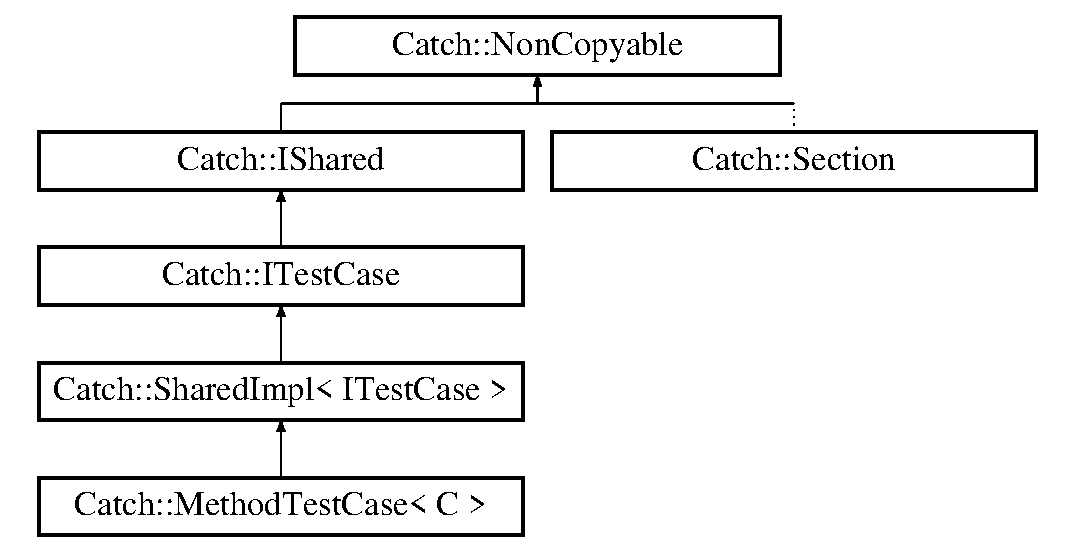
\includegraphics[height=5.000000cm]{class_catch_1_1_non_copyable}
\end{center}
\end{figure}
\subsection*{Protected Member Functions}
\begin{DoxyCompactItemize}
\item 
\mbox{\hyperlink{class_catch_1_1_non_copyable_a4b492dd5753f9952350fb64dc6cb9fe2}{Non\+Copyable}} ()
\item 
virtual \mbox{\hyperlink{class_catch_1_1_non_copyable_a81254677280fef337eb4a676e91e3293}{$\sim$\+Non\+Copyable}} ()
\end{DoxyCompactItemize}


\subsection{Constructor \& Destructor Documentation}
\mbox{\Hypertarget{class_catch_1_1_non_copyable_a4b492dd5753f9952350fb64dc6cb9fe2}\label{class_catch_1_1_non_copyable_a4b492dd5753f9952350fb64dc6cb9fe2}} 
\index{Catch\+::\+Non\+Copyable@{Catch\+::\+Non\+Copyable}!Non\+Copyable@{Non\+Copyable}}
\index{Non\+Copyable@{Non\+Copyable}!Catch\+::\+Non\+Copyable@{Catch\+::\+Non\+Copyable}}
\subsubsection{\texorpdfstring{Non\+Copyable()}{NonCopyable()}}
{\footnotesize\ttfamily Catch\+::\+Non\+Copyable\+::\+Non\+Copyable (\begin{DoxyParamCaption}{ }\end{DoxyParamCaption})\hspace{0.3cm}{\ttfamily [inline]}, {\ttfamily [protected]}}

\mbox{\Hypertarget{class_catch_1_1_non_copyable_a81254677280fef337eb4a676e91e3293}\label{class_catch_1_1_non_copyable_a81254677280fef337eb4a676e91e3293}} 
\index{Catch\+::\+Non\+Copyable@{Catch\+::\+Non\+Copyable}!````~Non\+Copyable@{$\sim$\+Non\+Copyable}}
\index{````~Non\+Copyable@{$\sim$\+Non\+Copyable}!Catch\+::\+Non\+Copyable@{Catch\+::\+Non\+Copyable}}
\subsubsection{\texorpdfstring{$\sim$\+Non\+Copyable()}{~NonCopyable()}}
{\footnotesize\ttfamily virtual Catch\+::\+Non\+Copyable\+::$\sim$\+Non\+Copyable (\begin{DoxyParamCaption}{ }\end{DoxyParamCaption})\hspace{0.3cm}{\ttfamily [protected]}, {\ttfamily [virtual]}}



The documentation for this class was generated from the following file\+:\begin{DoxyCompactItemize}
\item 
include/\mbox{\hyperlink{catch_8hpp}{catch.\+hpp}}\end{DoxyCompactItemize}

\hypertarget{class_catch_1_1_not_implemented_exception}{}\section{Catch\+:\+:Not\+Implemented\+Exception Class Reference}
\label{class_catch_1_1_not_implemented_exception}\index{Catch\+::\+Not\+Implemented\+Exception@{Catch\+::\+Not\+Implemented\+Exception}}


{\ttfamily \#include $<$catch.\+hpp$>$}

Inheritance diagram for Catch\+:\+:Not\+Implemented\+Exception\+:\begin{figure}[H]
\begin{center}
\leavevmode
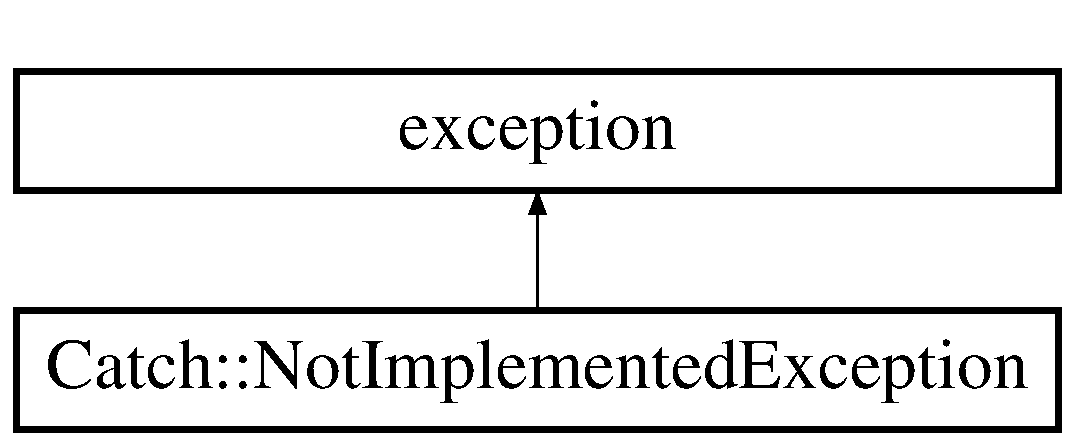
\includegraphics[height=2.000000cm]{class_catch_1_1_not_implemented_exception}
\end{center}
\end{figure}
\subsection*{Public Member Functions}
\begin{DoxyCompactItemize}
\item 
\mbox{\hyperlink{class_catch_1_1_not_implemented_exception_ab4f0a5c39d8ffb72c664e2c07e180634}{Not\+Implemented\+Exception}} (\mbox{\hyperlink{struct_catch_1_1_source_line_info}{Source\+Line\+Info}} const \&line\+Info)
\item 
\mbox{\hyperlink{class_catch_1_1_not_implemented_exception_a508a7a833455da2d3c10ea1a9d45e982}{Not\+Implemented\+Exception}} (\mbox{\hyperlink{class_catch_1_1_not_implemented_exception}{Not\+Implemented\+Exception}} const \&)
\item 
virtual \mbox{\hyperlink{class_catch_1_1_not_implemented_exception_a557e7312aaa32c37bded019f2b059bcb}{$\sim$\+Not\+Implemented\+Exception}} () \mbox{\hyperlink{catch_8hpp_a0408e94ca73880d41f38852b68eadb3c}{C\+A\+T\+C\+H\+\_\+\+N\+O\+E\+X\+C\+E\+PT}}
\item 
virtual const char $\ast$ \mbox{\hyperlink{class_catch_1_1_not_implemented_exception_ad4c13963f1a8feacda0cd331adda89e3}{what}} () const \mbox{\hyperlink{catch_8hpp_a0408e94ca73880d41f38852b68eadb3c}{C\+A\+T\+C\+H\+\_\+\+N\+O\+E\+X\+C\+E\+PT}}
\end{DoxyCompactItemize}


\subsection{Constructor \& Destructor Documentation}
\mbox{\Hypertarget{class_catch_1_1_not_implemented_exception_ab4f0a5c39d8ffb72c664e2c07e180634}\label{class_catch_1_1_not_implemented_exception_ab4f0a5c39d8ffb72c664e2c07e180634}} 
\index{Catch\+::\+Not\+Implemented\+Exception@{Catch\+::\+Not\+Implemented\+Exception}!Not\+Implemented\+Exception@{Not\+Implemented\+Exception}}
\index{Not\+Implemented\+Exception@{Not\+Implemented\+Exception}!Catch\+::\+Not\+Implemented\+Exception@{Catch\+::\+Not\+Implemented\+Exception}}
\subsubsection{\texorpdfstring{Not\+Implemented\+Exception()}{NotImplementedException()}\hspace{0.1cm}{\footnotesize\ttfamily [1/2]}}
{\footnotesize\ttfamily Catch\+::\+Not\+Implemented\+Exception\+::\+Not\+Implemented\+Exception (\begin{DoxyParamCaption}\item[{\mbox{\hyperlink{struct_catch_1_1_source_line_info}{Source\+Line\+Info}} const \&}]{line\+Info }\end{DoxyParamCaption})}

\mbox{\Hypertarget{class_catch_1_1_not_implemented_exception_a508a7a833455da2d3c10ea1a9d45e982}\label{class_catch_1_1_not_implemented_exception_a508a7a833455da2d3c10ea1a9d45e982}} 
\index{Catch\+::\+Not\+Implemented\+Exception@{Catch\+::\+Not\+Implemented\+Exception}!Not\+Implemented\+Exception@{Not\+Implemented\+Exception}}
\index{Not\+Implemented\+Exception@{Not\+Implemented\+Exception}!Catch\+::\+Not\+Implemented\+Exception@{Catch\+::\+Not\+Implemented\+Exception}}
\subsubsection{\texorpdfstring{Not\+Implemented\+Exception()}{NotImplementedException()}\hspace{0.1cm}{\footnotesize\ttfamily [2/2]}}
{\footnotesize\ttfamily Catch\+::\+Not\+Implemented\+Exception\+::\+Not\+Implemented\+Exception (\begin{DoxyParamCaption}\item[{\mbox{\hyperlink{class_catch_1_1_not_implemented_exception}{Not\+Implemented\+Exception}} const \&}]{ }\end{DoxyParamCaption})\hspace{0.3cm}{\ttfamily [inline]}}

\mbox{\Hypertarget{class_catch_1_1_not_implemented_exception_a557e7312aaa32c37bded019f2b059bcb}\label{class_catch_1_1_not_implemented_exception_a557e7312aaa32c37bded019f2b059bcb}} 
\index{Catch\+::\+Not\+Implemented\+Exception@{Catch\+::\+Not\+Implemented\+Exception}!````~Not\+Implemented\+Exception@{$\sim$\+Not\+Implemented\+Exception}}
\index{````~Not\+Implemented\+Exception@{$\sim$\+Not\+Implemented\+Exception}!Catch\+::\+Not\+Implemented\+Exception@{Catch\+::\+Not\+Implemented\+Exception}}
\subsubsection{\texorpdfstring{$\sim$\+Not\+Implemented\+Exception()}{~NotImplementedException()}}
{\footnotesize\ttfamily virtual Catch\+::\+Not\+Implemented\+Exception\+::$\sim$\+Not\+Implemented\+Exception (\begin{DoxyParamCaption}{ }\end{DoxyParamCaption})\hspace{0.3cm}{\ttfamily [inline]}, {\ttfamily [virtual]}}



\subsection{Member Function Documentation}
\mbox{\Hypertarget{class_catch_1_1_not_implemented_exception_ad4c13963f1a8feacda0cd331adda89e3}\label{class_catch_1_1_not_implemented_exception_ad4c13963f1a8feacda0cd331adda89e3}} 
\index{Catch\+::\+Not\+Implemented\+Exception@{Catch\+::\+Not\+Implemented\+Exception}!what@{what}}
\index{what@{what}!Catch\+::\+Not\+Implemented\+Exception@{Catch\+::\+Not\+Implemented\+Exception}}
\subsubsection{\texorpdfstring{what()}{what()}}
{\footnotesize\ttfamily virtual const char$\ast$ Catch\+::\+Not\+Implemented\+Exception\+::what (\begin{DoxyParamCaption}{ }\end{DoxyParamCaption}) const\hspace{0.3cm}{\ttfamily [virtual]}}



The documentation for this class was generated from the following file\+:\begin{DoxyCompactItemize}
\item 
include/\mbox{\hyperlink{catch_8hpp}{catch.\+hpp}}\end{DoxyCompactItemize}

\hypertarget{struct_catch_1_1_internal_1_1_operator_traits}{}\section{Catch\+:\+:Internal\+:\+:Operator\+Traits$<$ Op $>$ Struct Template Reference}
\label{struct_catch_1_1_internal_1_1_operator_traits}\index{Catch\+::\+Internal\+::\+Operator\+Traits$<$ Op $>$@{Catch\+::\+Internal\+::\+Operator\+Traits$<$ Op $>$}}


{\ttfamily \#include $<$catch.\+hpp$>$}

\subsection*{Static Public Member Functions}
\begin{DoxyCompactItemize}
\item 
static const char $\ast$ \mbox{\hyperlink{struct_catch_1_1_internal_1_1_operator_traits_ac6d08082ea33348d42bc4ccbd6d07671}{get\+Name}} ()
\end{DoxyCompactItemize}


\subsection{Member Function Documentation}
\mbox{\Hypertarget{struct_catch_1_1_internal_1_1_operator_traits_ac6d08082ea33348d42bc4ccbd6d07671}\label{struct_catch_1_1_internal_1_1_operator_traits_ac6d08082ea33348d42bc4ccbd6d07671}} 
\index{Catch\+::\+Internal\+::\+Operator\+Traits@{Catch\+::\+Internal\+::\+Operator\+Traits}!get\+Name@{get\+Name}}
\index{get\+Name@{get\+Name}!Catch\+::\+Internal\+::\+Operator\+Traits@{Catch\+::\+Internal\+::\+Operator\+Traits}}
\subsubsection{\texorpdfstring{get\+Name()}{getName()}}
{\footnotesize\ttfamily template$<$Operator Op$>$ \\
static const char$\ast$ \mbox{\hyperlink{struct_catch_1_1_internal_1_1_operator_traits}{Catch\+::\+Internal\+::\+Operator\+Traits}}$<$ Op $>$\+::get\+Name (\begin{DoxyParamCaption}{ }\end{DoxyParamCaption})\hspace{0.3cm}{\ttfamily [inline]}, {\ttfamily [static]}}



The documentation for this struct was generated from the following file\+:\begin{DoxyCompactItemize}
\item 
include/\mbox{\hyperlink{catch_8hpp}{catch.\+hpp}}\end{DoxyCompactItemize}

\hypertarget{struct_catch_1_1_internal_1_1_operator_traits_3_01_is_equal_to_01_4}{}\section{Catch\+:\+:Internal\+:\+:Operator\+Traits$<$ Is\+Equal\+To $>$ Struct Template Reference}
\label{struct_catch_1_1_internal_1_1_operator_traits_3_01_is_equal_to_01_4}\index{Catch\+::\+Internal\+::\+Operator\+Traits$<$ Is\+Equal\+To $>$@{Catch\+::\+Internal\+::\+Operator\+Traits$<$ Is\+Equal\+To $>$}}


{\ttfamily \#include $<$catch.\+hpp$>$}

\subsection*{Static Public Member Functions}
\begin{DoxyCompactItemize}
\item 
static const char $\ast$ \mbox{\hyperlink{struct_catch_1_1_internal_1_1_operator_traits_3_01_is_equal_to_01_4_addf03ac66f0ed83abcc037a7a327d4f1}{get\+Name}} ()
\end{DoxyCompactItemize}


\subsection{Member Function Documentation}
\mbox{\Hypertarget{struct_catch_1_1_internal_1_1_operator_traits_3_01_is_equal_to_01_4_addf03ac66f0ed83abcc037a7a327d4f1}\label{struct_catch_1_1_internal_1_1_operator_traits_3_01_is_equal_to_01_4_addf03ac66f0ed83abcc037a7a327d4f1}} 
\index{Catch\+::\+Internal\+::\+Operator\+Traits$<$ Is\+Equal\+To $>$@{Catch\+::\+Internal\+::\+Operator\+Traits$<$ Is\+Equal\+To $>$}!get\+Name@{get\+Name}}
\index{get\+Name@{get\+Name}!Catch\+::\+Internal\+::\+Operator\+Traits$<$ Is\+Equal\+To $>$@{Catch\+::\+Internal\+::\+Operator\+Traits$<$ Is\+Equal\+To $>$}}
\subsubsection{\texorpdfstring{get\+Name()}{getName()}}
{\footnotesize\ttfamily static const char$\ast$ \mbox{\hyperlink{struct_catch_1_1_internal_1_1_operator_traits}{Catch\+::\+Internal\+::\+Operator\+Traits}}$<$ \mbox{\hyperlink{namespace_catch_1_1_internal_ae3f96598a7858155750bf38e7295d83ea30e0accba6ec8384f4383b04dd2a6a9e}{Is\+Equal\+To}} $>$\+::get\+Name (\begin{DoxyParamCaption}{ }\end{DoxyParamCaption})\hspace{0.3cm}{\ttfamily [inline]}, {\ttfamily [static]}}



The documentation for this struct was generated from the following file\+:\begin{DoxyCompactItemize}
\item 
include/\mbox{\hyperlink{catch_8hpp}{catch.\+hpp}}\end{DoxyCompactItemize}

\hypertarget{struct_catch_1_1_internal_1_1_operator_traits_3_01_is_greater_than_01_4}{}\section{Catch\+:\+:Internal\+:\+:Operator\+Traits$<$ Is\+Greater\+Than $>$ Struct Template Reference}
\label{struct_catch_1_1_internal_1_1_operator_traits_3_01_is_greater_than_01_4}\index{Catch\+::\+Internal\+::\+Operator\+Traits$<$ Is\+Greater\+Than $>$@{Catch\+::\+Internal\+::\+Operator\+Traits$<$ Is\+Greater\+Than $>$}}


{\ttfamily \#include $<$catch.\+hpp$>$}

\subsection*{Static Public Member Functions}
\begin{DoxyCompactItemize}
\item 
static const char $\ast$ \mbox{\hyperlink{struct_catch_1_1_internal_1_1_operator_traits_3_01_is_greater_than_01_4_ab917bfb9ccbe461dc684ee5a34d67d27}{get\+Name}} ()
\end{DoxyCompactItemize}


\subsection{Member Function Documentation}
\mbox{\Hypertarget{struct_catch_1_1_internal_1_1_operator_traits_3_01_is_greater_than_01_4_ab917bfb9ccbe461dc684ee5a34d67d27}\label{struct_catch_1_1_internal_1_1_operator_traits_3_01_is_greater_than_01_4_ab917bfb9ccbe461dc684ee5a34d67d27}} 
\index{Catch\+::\+Internal\+::\+Operator\+Traits$<$ Is\+Greater\+Than $>$@{Catch\+::\+Internal\+::\+Operator\+Traits$<$ Is\+Greater\+Than $>$}!get\+Name@{get\+Name}}
\index{get\+Name@{get\+Name}!Catch\+::\+Internal\+::\+Operator\+Traits$<$ Is\+Greater\+Than $>$@{Catch\+::\+Internal\+::\+Operator\+Traits$<$ Is\+Greater\+Than $>$}}
\subsubsection{\texorpdfstring{get\+Name()}{getName()}}
{\footnotesize\ttfamily static const char$\ast$ \mbox{\hyperlink{struct_catch_1_1_internal_1_1_operator_traits}{Catch\+::\+Internal\+::\+Operator\+Traits}}$<$ \mbox{\hyperlink{namespace_catch_1_1_internal_ae3f96598a7858155750bf38e7295d83eac0e8866139e99803d169595af70f6c22}{Is\+Greater\+Than}} $>$\+::get\+Name (\begin{DoxyParamCaption}{ }\end{DoxyParamCaption})\hspace{0.3cm}{\ttfamily [inline]}, {\ttfamily [static]}}



The documentation for this struct was generated from the following file\+:\begin{DoxyCompactItemize}
\item 
include/\mbox{\hyperlink{catch_8hpp}{catch.\+hpp}}\end{DoxyCompactItemize}

\hypertarget{struct_catch_1_1_internal_1_1_operator_traits_3_01_is_greater_than_or_equal_to_01_4}{}\section{Catch\+:\+:Internal\+:\+:Operator\+Traits$<$ Is\+Greater\+Than\+Or\+Equal\+To $>$ Struct Template Reference}
\label{struct_catch_1_1_internal_1_1_operator_traits_3_01_is_greater_than_or_equal_to_01_4}\index{Catch\+::\+Internal\+::\+Operator\+Traits$<$ Is\+Greater\+Than\+Or\+Equal\+To $>$@{Catch\+::\+Internal\+::\+Operator\+Traits$<$ Is\+Greater\+Than\+Or\+Equal\+To $>$}}


{\ttfamily \#include $<$catch.\+hpp$>$}

\subsection*{Static Public Member Functions}
\begin{DoxyCompactItemize}
\item 
static const char $\ast$ \mbox{\hyperlink{struct_catch_1_1_internal_1_1_operator_traits_3_01_is_greater_than_or_equal_to_01_4_a76b6f6b0dbaf7d19ebb1b4b4891e719e}{get\+Name}} ()
\end{DoxyCompactItemize}


\subsection{Member Function Documentation}
\mbox{\Hypertarget{struct_catch_1_1_internal_1_1_operator_traits_3_01_is_greater_than_or_equal_to_01_4_a76b6f6b0dbaf7d19ebb1b4b4891e719e}\label{struct_catch_1_1_internal_1_1_operator_traits_3_01_is_greater_than_or_equal_to_01_4_a76b6f6b0dbaf7d19ebb1b4b4891e719e}} 
\index{Catch\+::\+Internal\+::\+Operator\+Traits$<$ Is\+Greater\+Than\+Or\+Equal\+To $>$@{Catch\+::\+Internal\+::\+Operator\+Traits$<$ Is\+Greater\+Than\+Or\+Equal\+To $>$}!get\+Name@{get\+Name}}
\index{get\+Name@{get\+Name}!Catch\+::\+Internal\+::\+Operator\+Traits$<$ Is\+Greater\+Than\+Or\+Equal\+To $>$@{Catch\+::\+Internal\+::\+Operator\+Traits$<$ Is\+Greater\+Than\+Or\+Equal\+To $>$}}
\subsubsection{\texorpdfstring{get\+Name()}{getName()}}
{\footnotesize\ttfamily static const char$\ast$ \mbox{\hyperlink{struct_catch_1_1_internal_1_1_operator_traits}{Catch\+::\+Internal\+::\+Operator\+Traits}}$<$ \mbox{\hyperlink{namespace_catch_1_1_internal_ae3f96598a7858155750bf38e7295d83ead2de7e9565e59e36c0987e402203ce1c}{Is\+Greater\+Than\+Or\+Equal\+To}} $>$\+::get\+Name (\begin{DoxyParamCaption}{ }\end{DoxyParamCaption})\hspace{0.3cm}{\ttfamily [inline]}, {\ttfamily [static]}}



The documentation for this struct was generated from the following file\+:\begin{DoxyCompactItemize}
\item 
include/\mbox{\hyperlink{catch_8hpp}{catch.\+hpp}}\end{DoxyCompactItemize}

\hypertarget{struct_catch_1_1_internal_1_1_operator_traits_3_01_is_less_than_01_4}{}\section{Catch\+:\+:Internal\+:\+:Operator\+Traits$<$ Is\+Less\+Than $>$ Struct Template Reference}
\label{struct_catch_1_1_internal_1_1_operator_traits_3_01_is_less_than_01_4}\index{Catch\+::\+Internal\+::\+Operator\+Traits$<$ Is\+Less\+Than $>$@{Catch\+::\+Internal\+::\+Operator\+Traits$<$ Is\+Less\+Than $>$}}


{\ttfamily \#include $<$catch.\+hpp$>$}

\subsection*{Static Public Member Functions}
\begin{DoxyCompactItemize}
\item 
static const char $\ast$ \mbox{\hyperlink{struct_catch_1_1_internal_1_1_operator_traits_3_01_is_less_than_01_4_aa3b536ddbd2e34b1253931ff00c32712}{get\+Name}} ()
\end{DoxyCompactItemize}


\subsection{Member Function Documentation}
\mbox{\Hypertarget{struct_catch_1_1_internal_1_1_operator_traits_3_01_is_less_than_01_4_aa3b536ddbd2e34b1253931ff00c32712}\label{struct_catch_1_1_internal_1_1_operator_traits_3_01_is_less_than_01_4_aa3b536ddbd2e34b1253931ff00c32712}} 
\index{Catch\+::\+Internal\+::\+Operator\+Traits$<$ Is\+Less\+Than $>$@{Catch\+::\+Internal\+::\+Operator\+Traits$<$ Is\+Less\+Than $>$}!get\+Name@{get\+Name}}
\index{get\+Name@{get\+Name}!Catch\+::\+Internal\+::\+Operator\+Traits$<$ Is\+Less\+Than $>$@{Catch\+::\+Internal\+::\+Operator\+Traits$<$ Is\+Less\+Than $>$}}
\subsubsection{\texorpdfstring{get\+Name()}{getName()}}
{\footnotesize\ttfamily static const char$\ast$ \mbox{\hyperlink{struct_catch_1_1_internal_1_1_operator_traits}{Catch\+::\+Internal\+::\+Operator\+Traits}}$<$ \mbox{\hyperlink{namespace_catch_1_1_internal_ae3f96598a7858155750bf38e7295d83eabbbfc41706595e50acbefa8408004b93}{Is\+Less\+Than}} $>$\+::get\+Name (\begin{DoxyParamCaption}{ }\end{DoxyParamCaption})\hspace{0.3cm}{\ttfamily [inline]}, {\ttfamily [static]}}



The documentation for this struct was generated from the following file\+:\begin{DoxyCompactItemize}
\item 
include/\mbox{\hyperlink{catch_8hpp}{catch.\+hpp}}\end{DoxyCompactItemize}

\hypertarget{struct_catch_1_1_internal_1_1_operator_traits_3_01_is_less_than_or_equal_to_01_4}{}\section{Catch\+:\+:Internal\+:\+:Operator\+Traits$<$ Is\+Less\+Than\+Or\+Equal\+To $>$ Struct Template Reference}
\label{struct_catch_1_1_internal_1_1_operator_traits_3_01_is_less_than_or_equal_to_01_4}\index{Catch\+::\+Internal\+::\+Operator\+Traits$<$ Is\+Less\+Than\+Or\+Equal\+To $>$@{Catch\+::\+Internal\+::\+Operator\+Traits$<$ Is\+Less\+Than\+Or\+Equal\+To $>$}}


{\ttfamily \#include $<$catch.\+hpp$>$}

\subsection*{Static Public Member Functions}
\begin{DoxyCompactItemize}
\item 
static const char $\ast$ \mbox{\hyperlink{struct_catch_1_1_internal_1_1_operator_traits_3_01_is_less_than_or_equal_to_01_4_ae8578813bc847838f10448c1541a9d7b}{get\+Name}} ()
\end{DoxyCompactItemize}


\subsection{Member Function Documentation}
\mbox{\Hypertarget{struct_catch_1_1_internal_1_1_operator_traits_3_01_is_less_than_or_equal_to_01_4_ae8578813bc847838f10448c1541a9d7b}\label{struct_catch_1_1_internal_1_1_operator_traits_3_01_is_less_than_or_equal_to_01_4_ae8578813bc847838f10448c1541a9d7b}} 
\index{Catch\+::\+Internal\+::\+Operator\+Traits$<$ Is\+Less\+Than\+Or\+Equal\+To $>$@{Catch\+::\+Internal\+::\+Operator\+Traits$<$ Is\+Less\+Than\+Or\+Equal\+To $>$}!get\+Name@{get\+Name}}
\index{get\+Name@{get\+Name}!Catch\+::\+Internal\+::\+Operator\+Traits$<$ Is\+Less\+Than\+Or\+Equal\+To $>$@{Catch\+::\+Internal\+::\+Operator\+Traits$<$ Is\+Less\+Than\+Or\+Equal\+To $>$}}
\subsubsection{\texorpdfstring{get\+Name()}{getName()}}
{\footnotesize\ttfamily static const char$\ast$ \mbox{\hyperlink{struct_catch_1_1_internal_1_1_operator_traits}{Catch\+::\+Internal\+::\+Operator\+Traits}}$<$ \mbox{\hyperlink{namespace_catch_1_1_internal_ae3f96598a7858155750bf38e7295d83ea0db29a4c3f1e81260036c5e27a8407fd}{Is\+Less\+Than\+Or\+Equal\+To}} $>$\+::get\+Name (\begin{DoxyParamCaption}{ }\end{DoxyParamCaption})\hspace{0.3cm}{\ttfamily [inline]}, {\ttfamily [static]}}



The documentation for this struct was generated from the following file\+:\begin{DoxyCompactItemize}
\item 
include/\mbox{\hyperlink{catch_8hpp}{catch.\+hpp}}\end{DoxyCompactItemize}

\hypertarget{struct_catch_1_1_internal_1_1_operator_traits_3_01_is_not_equal_to_01_4}{}\section{Catch\+:\+:Internal\+:\+:Operator\+Traits$<$ Is\+Not\+Equal\+To $>$ Struct Template Reference}
\label{struct_catch_1_1_internal_1_1_operator_traits_3_01_is_not_equal_to_01_4}\index{Catch\+::\+Internal\+::\+Operator\+Traits$<$ Is\+Not\+Equal\+To $>$@{Catch\+::\+Internal\+::\+Operator\+Traits$<$ Is\+Not\+Equal\+To $>$}}


{\ttfamily \#include $<$catch.\+hpp$>$}

\subsection*{Static Public Member Functions}
\begin{DoxyCompactItemize}
\item 
static const char $\ast$ \mbox{\hyperlink{struct_catch_1_1_internal_1_1_operator_traits_3_01_is_not_equal_to_01_4_a54a795b8bf7c80a9fdbc7b81f39133b4}{get\+Name}} ()
\end{DoxyCompactItemize}


\subsection{Member Function Documentation}
\mbox{\Hypertarget{struct_catch_1_1_internal_1_1_operator_traits_3_01_is_not_equal_to_01_4_a54a795b8bf7c80a9fdbc7b81f39133b4}\label{struct_catch_1_1_internal_1_1_operator_traits_3_01_is_not_equal_to_01_4_a54a795b8bf7c80a9fdbc7b81f39133b4}} 
\index{Catch\+::\+Internal\+::\+Operator\+Traits$<$ Is\+Not\+Equal\+To $>$@{Catch\+::\+Internal\+::\+Operator\+Traits$<$ Is\+Not\+Equal\+To $>$}!get\+Name@{get\+Name}}
\index{get\+Name@{get\+Name}!Catch\+::\+Internal\+::\+Operator\+Traits$<$ Is\+Not\+Equal\+To $>$@{Catch\+::\+Internal\+::\+Operator\+Traits$<$ Is\+Not\+Equal\+To $>$}}
\subsubsection{\texorpdfstring{get\+Name()}{getName()}}
{\footnotesize\ttfamily static const char$\ast$ \mbox{\hyperlink{struct_catch_1_1_internal_1_1_operator_traits}{Catch\+::\+Internal\+::\+Operator\+Traits}}$<$ \mbox{\hyperlink{namespace_catch_1_1_internal_ae3f96598a7858155750bf38e7295d83ea1e1699cf7d3dbee0908f1a123da2456d}{Is\+Not\+Equal\+To}} $>$\+::get\+Name (\begin{DoxyParamCaption}{ }\end{DoxyParamCaption})\hspace{0.3cm}{\ttfamily [inline]}, {\ttfamily [static]}}



The documentation for this struct was generated from the following file\+:\begin{DoxyCompactItemize}
\item 
include/\mbox{\hyperlink{catch_8hpp}{catch.\+hpp}}\end{DoxyCompactItemize}

\hypertarget{class_catch_1_1_option}{}\section{Catch\+:\+:Option$<$ T $>$ Class Template Reference}
\label{class_catch_1_1_option}\index{Catch\+::\+Option$<$ T $>$@{Catch\+::\+Option$<$ T $>$}}


{\ttfamily \#include $<$catch.\+hpp$>$}

\subsection*{Public Member Functions}
\begin{DoxyCompactItemize}
\item 
\mbox{\hyperlink{class_catch_1_1_option_a8efb01b593d798decc80cbbdf311f2a3}{Option}} ()
\item 
\mbox{\hyperlink{class_catch_1_1_option_a5aeb9c22d48a6882bdf5fb4730b06c86}{Option}} (T const \&\+\_\+value)
\item 
\mbox{\hyperlink{class_catch_1_1_option_af02f2e4559f06384baec0def8c68c5fd}{Option}} (\mbox{\hyperlink{class_catch_1_1_option}{Option}} const \&\+\_\+other)
\item 
\mbox{\hyperlink{class_catch_1_1_option_a37fe90bb47bb909f150a5ad6be25581a}{$\sim$\+Option}} ()
\item 
\mbox{\hyperlink{class_catch_1_1_option}{Option}} \& \mbox{\hyperlink{class_catch_1_1_option_a78c65b15dd6b2fbd04c5012c43017c8f}{operator=}} (\mbox{\hyperlink{class_catch_1_1_option}{Option}} const \&\+\_\+other)
\item 
\mbox{\hyperlink{class_catch_1_1_option}{Option}} \& \mbox{\hyperlink{class_catch_1_1_option_a2be7e343ab22d6061726d32ab4622653}{operator=}} (T const \&\+\_\+value)
\item 
void \mbox{\hyperlink{class_catch_1_1_option_a37b4e0e5d4d56296adacd267a616f4e0}{reset}} ()
\item 
T \& \mbox{\hyperlink{class_catch_1_1_option_afd989852fa453731c3190dac63caccb0}{operator$\ast$}} ()
\item 
T const  \& \mbox{\hyperlink{class_catch_1_1_option_a734fc9c2eb1a1f7f8e8f6a4eb12160f0}{operator$\ast$}} () const
\item 
T $\ast$ \mbox{\hyperlink{class_catch_1_1_option_acad340798a16c8f700f8763119e90f31}{operator-\/$>$}} ()
\item 
const T $\ast$ \mbox{\hyperlink{class_catch_1_1_option_ae8343cbc36dbb95b2dce333d2a6fdc28}{operator-\/$>$}} () const
\item 
T \mbox{\hyperlink{class_catch_1_1_option_a8d9ae2e30b0eb76fe134a6fbc8423124}{value\+Or}} (T const \&default\+Value) const
\item 
bool \mbox{\hyperlink{class_catch_1_1_option_a97c95829afbe92f2bcc5fd75b32c0825}{some}} () const
\item 
bool \mbox{\hyperlink{class_catch_1_1_option_a821753afdc3fac947a13a01fbe0d248e}{none}} () const
\item 
bool \mbox{\hyperlink{class_catch_1_1_option_a96dccb86bdf45ee0c08e122b6133bef3}{operator!}} () const
\item 
\mbox{\hyperlink{class_catch_1_1_option_a8ed8de7b072f893c85df14913dbbe197}{operator Safe\+Bool\+::type}} () const
\end{DoxyCompactItemize}


\subsection{Constructor \& Destructor Documentation}
\mbox{\Hypertarget{class_catch_1_1_option_a8efb01b593d798decc80cbbdf311f2a3}\label{class_catch_1_1_option_a8efb01b593d798decc80cbbdf311f2a3}} 
\index{Catch\+::\+Option@{Catch\+::\+Option}!Option@{Option}}
\index{Option@{Option}!Catch\+::\+Option@{Catch\+::\+Option}}
\subsubsection{\texorpdfstring{Option()}{Option()}\hspace{0.1cm}{\footnotesize\ttfamily [1/3]}}
{\footnotesize\ttfamily template$<$typename T $>$ \\
\mbox{\hyperlink{class_catch_1_1_option}{Catch\+::\+Option}}$<$ T $>$\+::\mbox{\hyperlink{class_catch_1_1_option}{Option}} (\begin{DoxyParamCaption}{ }\end{DoxyParamCaption})\hspace{0.3cm}{\ttfamily [inline]}}

\mbox{\Hypertarget{class_catch_1_1_option_a5aeb9c22d48a6882bdf5fb4730b06c86}\label{class_catch_1_1_option_a5aeb9c22d48a6882bdf5fb4730b06c86}} 
\index{Catch\+::\+Option@{Catch\+::\+Option}!Option@{Option}}
\index{Option@{Option}!Catch\+::\+Option@{Catch\+::\+Option}}
\subsubsection{\texorpdfstring{Option()}{Option()}\hspace{0.1cm}{\footnotesize\ttfamily [2/3]}}
{\footnotesize\ttfamily template$<$typename T $>$ \\
\mbox{\hyperlink{class_catch_1_1_option}{Catch\+::\+Option}}$<$ T $>$\+::\mbox{\hyperlink{class_catch_1_1_option}{Option}} (\begin{DoxyParamCaption}\item[{T const \&}]{\+\_\+value }\end{DoxyParamCaption})\hspace{0.3cm}{\ttfamily [inline]}}

\mbox{\Hypertarget{class_catch_1_1_option_af02f2e4559f06384baec0def8c68c5fd}\label{class_catch_1_1_option_af02f2e4559f06384baec0def8c68c5fd}} 
\index{Catch\+::\+Option@{Catch\+::\+Option}!Option@{Option}}
\index{Option@{Option}!Catch\+::\+Option@{Catch\+::\+Option}}
\subsubsection{\texorpdfstring{Option()}{Option()}\hspace{0.1cm}{\footnotesize\ttfamily [3/3]}}
{\footnotesize\ttfamily template$<$typename T $>$ \\
\mbox{\hyperlink{class_catch_1_1_option}{Catch\+::\+Option}}$<$ T $>$\+::\mbox{\hyperlink{class_catch_1_1_option}{Option}} (\begin{DoxyParamCaption}\item[{\mbox{\hyperlink{class_catch_1_1_option}{Option}}$<$ T $>$ const \&}]{\+\_\+other }\end{DoxyParamCaption})\hspace{0.3cm}{\ttfamily [inline]}}

\mbox{\Hypertarget{class_catch_1_1_option_a37fe90bb47bb909f150a5ad6be25581a}\label{class_catch_1_1_option_a37fe90bb47bb909f150a5ad6be25581a}} 
\index{Catch\+::\+Option@{Catch\+::\+Option}!````~Option@{$\sim$\+Option}}
\index{````~Option@{$\sim$\+Option}!Catch\+::\+Option@{Catch\+::\+Option}}
\subsubsection{\texorpdfstring{$\sim$\+Option()}{~Option()}}
{\footnotesize\ttfamily template$<$typename T $>$ \\
\mbox{\hyperlink{class_catch_1_1_option}{Catch\+::\+Option}}$<$ T $>$\+::$\sim$\mbox{\hyperlink{class_catch_1_1_option}{Option}} (\begin{DoxyParamCaption}{ }\end{DoxyParamCaption})\hspace{0.3cm}{\ttfamily [inline]}}



\subsection{Member Function Documentation}
\mbox{\Hypertarget{class_catch_1_1_option_a821753afdc3fac947a13a01fbe0d248e}\label{class_catch_1_1_option_a821753afdc3fac947a13a01fbe0d248e}} 
\index{Catch\+::\+Option@{Catch\+::\+Option}!none@{none}}
\index{none@{none}!Catch\+::\+Option@{Catch\+::\+Option}}
\subsubsection{\texorpdfstring{none()}{none()}}
{\footnotesize\ttfamily template$<$typename T $>$ \\
bool \mbox{\hyperlink{class_catch_1_1_option}{Catch\+::\+Option}}$<$ T $>$\+::none (\begin{DoxyParamCaption}{ }\end{DoxyParamCaption}) const\hspace{0.3cm}{\ttfamily [inline]}}

\mbox{\Hypertarget{class_catch_1_1_option_a8ed8de7b072f893c85df14913dbbe197}\label{class_catch_1_1_option_a8ed8de7b072f893c85df14913dbbe197}} 
\index{Catch\+::\+Option@{Catch\+::\+Option}!operator Safe\+Bool\+::type@{operator Safe\+Bool\+::type}}
\index{operator Safe\+Bool\+::type@{operator Safe\+Bool\+::type}!Catch\+::\+Option@{Catch\+::\+Option}}
\subsubsection{\texorpdfstring{operator Safe\+Bool\+::type()}{operator SafeBool::type()}}
{\footnotesize\ttfamily template$<$typename T $>$ \\
\mbox{\hyperlink{class_catch_1_1_option}{Catch\+::\+Option}}$<$ T $>$\+::operator \mbox{\hyperlink{class_catch_1_1_safe_bool_a39eef9baed296299d625a54d54a2a958}{Safe\+Bool\+::type}} (\begin{DoxyParamCaption}{ }\end{DoxyParamCaption}) const\hspace{0.3cm}{\ttfamily [inline]}}

\mbox{\Hypertarget{class_catch_1_1_option_a96dccb86bdf45ee0c08e122b6133bef3}\label{class_catch_1_1_option_a96dccb86bdf45ee0c08e122b6133bef3}} 
\index{Catch\+::\+Option@{Catch\+::\+Option}!operator"!@{operator"!}}
\index{operator"!@{operator"!}!Catch\+::\+Option@{Catch\+::\+Option}}
\subsubsection{\texorpdfstring{operator"!()}{operator!()}}
{\footnotesize\ttfamily template$<$typename T $>$ \\
bool \mbox{\hyperlink{class_catch_1_1_option}{Catch\+::\+Option}}$<$ T $>$\+::operator! (\begin{DoxyParamCaption}{ }\end{DoxyParamCaption}) const\hspace{0.3cm}{\ttfamily [inline]}}

\mbox{\Hypertarget{class_catch_1_1_option_afd989852fa453731c3190dac63caccb0}\label{class_catch_1_1_option_afd989852fa453731c3190dac63caccb0}} 
\index{Catch\+::\+Option@{Catch\+::\+Option}!operator$\ast$@{operator$\ast$}}
\index{operator$\ast$@{operator$\ast$}!Catch\+::\+Option@{Catch\+::\+Option}}
\subsubsection{\texorpdfstring{operator$\ast$()}{operator*()}\hspace{0.1cm}{\footnotesize\ttfamily [1/2]}}
{\footnotesize\ttfamily template$<$typename T $>$ \\
T\& \mbox{\hyperlink{class_catch_1_1_option}{Catch\+::\+Option}}$<$ T $>$\+::operator$\ast$ (\begin{DoxyParamCaption}{ }\end{DoxyParamCaption})\hspace{0.3cm}{\ttfamily [inline]}}

\mbox{\Hypertarget{class_catch_1_1_option_a734fc9c2eb1a1f7f8e8f6a4eb12160f0}\label{class_catch_1_1_option_a734fc9c2eb1a1f7f8e8f6a4eb12160f0}} 
\index{Catch\+::\+Option@{Catch\+::\+Option}!operator$\ast$@{operator$\ast$}}
\index{operator$\ast$@{operator$\ast$}!Catch\+::\+Option@{Catch\+::\+Option}}
\subsubsection{\texorpdfstring{operator$\ast$()}{operator*()}\hspace{0.1cm}{\footnotesize\ttfamily [2/2]}}
{\footnotesize\ttfamily template$<$typename T $>$ \\
T const\& \mbox{\hyperlink{class_catch_1_1_option}{Catch\+::\+Option}}$<$ T $>$\+::operator$\ast$ (\begin{DoxyParamCaption}{ }\end{DoxyParamCaption}) const\hspace{0.3cm}{\ttfamily [inline]}}

\mbox{\Hypertarget{class_catch_1_1_option_acad340798a16c8f700f8763119e90f31}\label{class_catch_1_1_option_acad340798a16c8f700f8763119e90f31}} 
\index{Catch\+::\+Option@{Catch\+::\+Option}!operator-\/$>$@{operator-\/$>$}}
\index{operator-\/$>$@{operator-\/$>$}!Catch\+::\+Option@{Catch\+::\+Option}}
\subsubsection{\texorpdfstring{operator-\/$>$()}{operator->()}\hspace{0.1cm}{\footnotesize\ttfamily [1/2]}}
{\footnotesize\ttfamily template$<$typename T $>$ \\
T$\ast$ \mbox{\hyperlink{class_catch_1_1_option}{Catch\+::\+Option}}$<$ T $>$\+::operator-\/$>$ (\begin{DoxyParamCaption}{ }\end{DoxyParamCaption})\hspace{0.3cm}{\ttfamily [inline]}}

\mbox{\Hypertarget{class_catch_1_1_option_ae8343cbc36dbb95b2dce333d2a6fdc28}\label{class_catch_1_1_option_ae8343cbc36dbb95b2dce333d2a6fdc28}} 
\index{Catch\+::\+Option@{Catch\+::\+Option}!operator-\/$>$@{operator-\/$>$}}
\index{operator-\/$>$@{operator-\/$>$}!Catch\+::\+Option@{Catch\+::\+Option}}
\subsubsection{\texorpdfstring{operator-\/$>$()}{operator->()}\hspace{0.1cm}{\footnotesize\ttfamily [2/2]}}
{\footnotesize\ttfamily template$<$typename T $>$ \\
const T$\ast$ \mbox{\hyperlink{class_catch_1_1_option}{Catch\+::\+Option}}$<$ T $>$\+::operator-\/$>$ (\begin{DoxyParamCaption}{ }\end{DoxyParamCaption}) const\hspace{0.3cm}{\ttfamily [inline]}}

\mbox{\Hypertarget{class_catch_1_1_option_a78c65b15dd6b2fbd04c5012c43017c8f}\label{class_catch_1_1_option_a78c65b15dd6b2fbd04c5012c43017c8f}} 
\index{Catch\+::\+Option@{Catch\+::\+Option}!operator=@{operator=}}
\index{operator=@{operator=}!Catch\+::\+Option@{Catch\+::\+Option}}
\subsubsection{\texorpdfstring{operator=()}{operator=()}\hspace{0.1cm}{\footnotesize\ttfamily [1/2]}}
{\footnotesize\ttfamily template$<$typename T $>$ \\
\mbox{\hyperlink{class_catch_1_1_option}{Option}}\& \mbox{\hyperlink{class_catch_1_1_option}{Catch\+::\+Option}}$<$ T $>$\+::operator= (\begin{DoxyParamCaption}\item[{\mbox{\hyperlink{class_catch_1_1_option}{Option}}$<$ T $>$ const \&}]{\+\_\+other }\end{DoxyParamCaption})\hspace{0.3cm}{\ttfamily [inline]}}

\mbox{\Hypertarget{class_catch_1_1_option_a2be7e343ab22d6061726d32ab4622653}\label{class_catch_1_1_option_a2be7e343ab22d6061726d32ab4622653}} 
\index{Catch\+::\+Option@{Catch\+::\+Option}!operator=@{operator=}}
\index{operator=@{operator=}!Catch\+::\+Option@{Catch\+::\+Option}}
\subsubsection{\texorpdfstring{operator=()}{operator=()}\hspace{0.1cm}{\footnotesize\ttfamily [2/2]}}
{\footnotesize\ttfamily template$<$typename T $>$ \\
\mbox{\hyperlink{class_catch_1_1_option}{Option}}\& \mbox{\hyperlink{class_catch_1_1_option}{Catch\+::\+Option}}$<$ T $>$\+::operator= (\begin{DoxyParamCaption}\item[{T const \&}]{\+\_\+value }\end{DoxyParamCaption})\hspace{0.3cm}{\ttfamily [inline]}}

\mbox{\Hypertarget{class_catch_1_1_option_a37b4e0e5d4d56296adacd267a616f4e0}\label{class_catch_1_1_option_a37b4e0e5d4d56296adacd267a616f4e0}} 
\index{Catch\+::\+Option@{Catch\+::\+Option}!reset@{reset}}
\index{reset@{reset}!Catch\+::\+Option@{Catch\+::\+Option}}
\subsubsection{\texorpdfstring{reset()}{reset()}}
{\footnotesize\ttfamily template$<$typename T $>$ \\
void \mbox{\hyperlink{class_catch_1_1_option}{Catch\+::\+Option}}$<$ T $>$\+::reset (\begin{DoxyParamCaption}{ }\end{DoxyParamCaption})\hspace{0.3cm}{\ttfamily [inline]}}

\mbox{\Hypertarget{class_catch_1_1_option_a97c95829afbe92f2bcc5fd75b32c0825}\label{class_catch_1_1_option_a97c95829afbe92f2bcc5fd75b32c0825}} 
\index{Catch\+::\+Option@{Catch\+::\+Option}!some@{some}}
\index{some@{some}!Catch\+::\+Option@{Catch\+::\+Option}}
\subsubsection{\texorpdfstring{some()}{some()}}
{\footnotesize\ttfamily template$<$typename T $>$ \\
bool \mbox{\hyperlink{class_catch_1_1_option}{Catch\+::\+Option}}$<$ T $>$\+::some (\begin{DoxyParamCaption}{ }\end{DoxyParamCaption}) const\hspace{0.3cm}{\ttfamily [inline]}}

\mbox{\Hypertarget{class_catch_1_1_option_a8d9ae2e30b0eb76fe134a6fbc8423124}\label{class_catch_1_1_option_a8d9ae2e30b0eb76fe134a6fbc8423124}} 
\index{Catch\+::\+Option@{Catch\+::\+Option}!value\+Or@{value\+Or}}
\index{value\+Or@{value\+Or}!Catch\+::\+Option@{Catch\+::\+Option}}
\subsubsection{\texorpdfstring{value\+Or()}{valueOr()}}
{\footnotesize\ttfamily template$<$typename T $>$ \\
T \mbox{\hyperlink{class_catch_1_1_option}{Catch\+::\+Option}}$<$ T $>$\+::value\+Or (\begin{DoxyParamCaption}\item[{T const \&}]{default\+Value }\end{DoxyParamCaption}) const\hspace{0.3cm}{\ttfamily [inline]}}



\subsection{Member Data Documentation}
\mbox{\Hypertarget{class_catch_1_1_option_a48ef08179923d6f943abe614999e6073}\label{class_catch_1_1_option_a48ef08179923d6f943abe614999e6073}} 
\index{Catch\+::\+Option@{Catch\+::\+Option}!dummy1@{dummy1}}
\index{dummy1@{dummy1}!Catch\+::\+Option@{Catch\+::\+Option}}
\subsubsection{\texorpdfstring{dummy1}{dummy1}}
{\footnotesize\ttfamily template$<$typename T $>$ \\
long double \mbox{\hyperlink{class_catch_1_1_option}{Catch\+::\+Option}}$<$ T $>$\+::dummy1}

\mbox{\Hypertarget{class_catch_1_1_option_afa73c2396b7732932a148b3c889b81d1}\label{class_catch_1_1_option_afa73c2396b7732932a148b3c889b81d1}} 
\index{Catch\+::\+Option@{Catch\+::\+Option}!dummy2@{dummy2}}
\index{dummy2@{dummy2}!Catch\+::\+Option@{Catch\+::\+Option}}
\subsubsection{\texorpdfstring{dummy2}{dummy2}}
{\footnotesize\ttfamily template$<$typename T $>$ \\
void($\ast$ \mbox{\hyperlink{class_catch_1_1_option}{Catch\+::\+Option}}$<$ T $>$\+::dummy2) ()}

\mbox{\Hypertarget{class_catch_1_1_option_a5540a84662093591be496c3a57e9da3f}\label{class_catch_1_1_option_a5540a84662093591be496c3a57e9da3f}} 
\index{Catch\+::\+Option@{Catch\+::\+Option}!dummy3@{dummy3}}
\index{dummy3@{dummy3}!Catch\+::\+Option@{Catch\+::\+Option}}
\subsubsection{\texorpdfstring{dummy3}{dummy3}}
{\footnotesize\ttfamily template$<$typename T $>$ \\
long double \mbox{\hyperlink{class_catch_1_1_option}{Catch\+::\+Option}}$<$ T $>$\+::dummy3}

\mbox{\Hypertarget{class_catch_1_1_option_acdebca1b18bb8542c3f676b8dd805f23}\label{class_catch_1_1_option_acdebca1b18bb8542c3f676b8dd805f23}} 
\index{Catch\+::\+Option@{Catch\+::\+Option}!storage@{storage}}
\index{storage@{storage}!Catch\+::\+Option@{Catch\+::\+Option}}
\subsubsection{\texorpdfstring{storage}{storage}}
{\footnotesize\ttfamily template$<$typename T $>$ \\
char \mbox{\hyperlink{class_catch_1_1_option}{Catch\+::\+Option}}$<$ T $>$\+::storage\mbox{[}sizeof(T)\mbox{]}}



The documentation for this class was generated from the following file\+:\begin{DoxyCompactItemize}
\item 
include/\mbox{\hyperlink{catch_8hpp}{catch.\+hpp}}\end{DoxyCompactItemize}

\hypertarget{struct_catch_1_1pluralise}{}\section{Catch\+:\+:pluralise Struct Reference}
\label{struct_catch_1_1pluralise}\index{Catch\+::pluralise@{Catch\+::pluralise}}


{\ttfamily \#include $<$catch.\+hpp$>$}

\subsection*{Public Member Functions}
\begin{DoxyCompactItemize}
\item 
\mbox{\hyperlink{struct_catch_1_1pluralise_a5c55e22de2416cfe416edf715c6b9234}{pluralise}} (std\+::size\+\_\+t count, std\+::string const \&label)
\end{DoxyCompactItemize}
\subsection*{Public Attributes}
\begin{DoxyCompactItemize}
\item 
std\+::size\+\_\+t \mbox{\hyperlink{struct_catch_1_1pluralise_a4dce2fa13ec6f00fac09b2418265441e}{m\+\_\+count}}
\item 
std\+::string \mbox{\hyperlink{struct_catch_1_1pluralise_a8849cbdd3f11ebe7747597c8644e8793}{m\+\_\+label}}
\end{DoxyCompactItemize}
\subsection*{Friends}
\begin{DoxyCompactItemize}
\item 
std\+::ostream \& \mbox{\hyperlink{struct_catch_1_1pluralise_aa7dac6b165514c1f85e0695d678fdef5}{operator$<$$<$}} (std\+::ostream \&os, \mbox{\hyperlink{struct_catch_1_1pluralise}{pluralise}} const \&pluraliser)
\end{DoxyCompactItemize}


\subsection{Constructor \& Destructor Documentation}
\mbox{\Hypertarget{struct_catch_1_1pluralise_a5c55e22de2416cfe416edf715c6b9234}\label{struct_catch_1_1pluralise_a5c55e22de2416cfe416edf715c6b9234}} 
\index{Catch\+::pluralise@{Catch\+::pluralise}!pluralise@{pluralise}}
\index{pluralise@{pluralise}!Catch\+::pluralise@{Catch\+::pluralise}}
\subsubsection{\texorpdfstring{pluralise()}{pluralise()}}
{\footnotesize\ttfamily Catch\+::pluralise\+::pluralise (\begin{DoxyParamCaption}\item[{std\+::size\+\_\+t}]{count,  }\item[{std\+::string const \&}]{label }\end{DoxyParamCaption})}



\subsection{Friends And Related Function Documentation}
\mbox{\Hypertarget{struct_catch_1_1pluralise_aa7dac6b165514c1f85e0695d678fdef5}\label{struct_catch_1_1pluralise_aa7dac6b165514c1f85e0695d678fdef5}} 
\index{Catch\+::pluralise@{Catch\+::pluralise}!operator$<$$<$@{operator$<$$<$}}
\index{operator$<$$<$@{operator$<$$<$}!Catch\+::pluralise@{Catch\+::pluralise}}
\subsubsection{\texorpdfstring{operator$<$$<$}{operator<<}}
{\footnotesize\ttfamily std\+::ostream\& operator$<$$<$ (\begin{DoxyParamCaption}\item[{std\+::ostream \&}]{os,  }\item[{\mbox{\hyperlink{struct_catch_1_1pluralise}{pluralise}} const \&}]{pluraliser }\end{DoxyParamCaption})\hspace{0.3cm}{\ttfamily [friend]}}



\subsection{Member Data Documentation}
\mbox{\Hypertarget{struct_catch_1_1pluralise_a4dce2fa13ec6f00fac09b2418265441e}\label{struct_catch_1_1pluralise_a4dce2fa13ec6f00fac09b2418265441e}} 
\index{Catch\+::pluralise@{Catch\+::pluralise}!m\+\_\+count@{m\+\_\+count}}
\index{m\+\_\+count@{m\+\_\+count}!Catch\+::pluralise@{Catch\+::pluralise}}
\subsubsection{\texorpdfstring{m\+\_\+count}{m\_count}}
{\footnotesize\ttfamily std\+::size\+\_\+t Catch\+::pluralise\+::m\+\_\+count}

\mbox{\Hypertarget{struct_catch_1_1pluralise_a8849cbdd3f11ebe7747597c8644e8793}\label{struct_catch_1_1pluralise_a8849cbdd3f11ebe7747597c8644e8793}} 
\index{Catch\+::pluralise@{Catch\+::pluralise}!m\+\_\+label@{m\+\_\+label}}
\index{m\+\_\+label@{m\+\_\+label}!Catch\+::pluralise@{Catch\+::pluralise}}
\subsubsection{\texorpdfstring{m\+\_\+label}{m\_label}}
{\footnotesize\ttfamily std\+::string Catch\+::pluralise\+::m\+\_\+label}



The documentation for this struct was generated from the following file\+:\begin{DoxyCompactItemize}
\item 
include/\mbox{\hyperlink{catch_8hpp}{catch.\+hpp}}\end{DoxyCompactItemize}

\hypertarget{class_catch_1_1_ptr}{}\section{Catch\+:\+:Ptr$<$ T $>$ Class Template Reference}
\label{class_catch_1_1_ptr}\index{Catch\+::\+Ptr$<$ T $>$@{Catch\+::\+Ptr$<$ T $>$}}


{\ttfamily \#include $<$catch.\+hpp$>$}

\subsection*{Public Member Functions}
\begin{DoxyCompactItemize}
\item 
\mbox{\hyperlink{class_catch_1_1_ptr_a6108f0195595ee9d7a411daea810beaf}{Ptr}} ()
\item 
\mbox{\hyperlink{class_catch_1_1_ptr_aacec063a79cd142e39040a31c6b3c40b}{Ptr}} (T $\ast$p)
\item 
\mbox{\hyperlink{class_catch_1_1_ptr_ac629dd8ebe5763a37bb89e6c1d6a1771}{Ptr}} (\mbox{\hyperlink{class_catch_1_1_ptr}{Ptr}} const \&other)
\item 
\mbox{\hyperlink{class_catch_1_1_ptr_ac96d3bb33adcfb983207385cfba5fe8a}{$\sim$\+Ptr}} ()
\item 
void \mbox{\hyperlink{class_catch_1_1_ptr_af8d0fa7a2cd20842830b354ac31dfe5c}{reset}} ()
\item 
\mbox{\hyperlink{class_catch_1_1_ptr}{Ptr}} \& \mbox{\hyperlink{class_catch_1_1_ptr_a9b08c868b447d679ed201921f5c94683}{operator=}} (T $\ast$p)
\item 
\mbox{\hyperlink{class_catch_1_1_ptr}{Ptr}} \& \mbox{\hyperlink{class_catch_1_1_ptr_af42074444c1bc6a70ebdc406a8617708}{operator=}} (\mbox{\hyperlink{class_catch_1_1_ptr}{Ptr}} const \&other)
\item 
void \mbox{\hyperlink{class_catch_1_1_ptr_a172bf8b4e71e26a5a4d92f5b02158b50}{swap}} (\mbox{\hyperlink{class_catch_1_1_ptr}{Ptr}} \&other)
\item 
T $\ast$ \mbox{\hyperlink{class_catch_1_1_ptr_a2158bb2a1a21b001a2e72d4591d3e31e}{get}} () const
\item 
T \& \mbox{\hyperlink{class_catch_1_1_ptr_a8d73989b1c77a1cab6152766feaa837f}{operator$\ast$}} () const
\item 
T $\ast$ \mbox{\hyperlink{class_catch_1_1_ptr_acc0996cbd99f360069260a898b3f4fda}{operator-\/$>$}} () const
\item 
bool \mbox{\hyperlink{class_catch_1_1_ptr_a85c4fe6cebf2a69d0416020b65714360}{operator!}} () const
\item 
\mbox{\hyperlink{class_catch_1_1_ptr_a102838cb25643586679e12efca26a3af}{operator Safe\+Bool\+::type}} () const
\end{DoxyCompactItemize}


\subsection{Constructor \& Destructor Documentation}
\mbox{\Hypertarget{class_catch_1_1_ptr_a6108f0195595ee9d7a411daea810beaf}\label{class_catch_1_1_ptr_a6108f0195595ee9d7a411daea810beaf}} 
\index{Catch\+::\+Ptr@{Catch\+::\+Ptr}!Ptr@{Ptr}}
\index{Ptr@{Ptr}!Catch\+::\+Ptr@{Catch\+::\+Ptr}}
\subsubsection{\texorpdfstring{Ptr()}{Ptr()}\hspace{0.1cm}{\footnotesize\ttfamily [1/3]}}
{\footnotesize\ttfamily template$<$typename T$>$ \\
\mbox{\hyperlink{class_catch_1_1_ptr}{Catch\+::\+Ptr}}$<$ T $>$\+::\mbox{\hyperlink{class_catch_1_1_ptr}{Ptr}} (\begin{DoxyParamCaption}{ }\end{DoxyParamCaption})\hspace{0.3cm}{\ttfamily [inline]}}

\mbox{\Hypertarget{class_catch_1_1_ptr_aacec063a79cd142e39040a31c6b3c40b}\label{class_catch_1_1_ptr_aacec063a79cd142e39040a31c6b3c40b}} 
\index{Catch\+::\+Ptr@{Catch\+::\+Ptr}!Ptr@{Ptr}}
\index{Ptr@{Ptr}!Catch\+::\+Ptr@{Catch\+::\+Ptr}}
\subsubsection{\texorpdfstring{Ptr()}{Ptr()}\hspace{0.1cm}{\footnotesize\ttfamily [2/3]}}
{\footnotesize\ttfamily template$<$typename T$>$ \\
\mbox{\hyperlink{class_catch_1_1_ptr}{Catch\+::\+Ptr}}$<$ T $>$\+::\mbox{\hyperlink{class_catch_1_1_ptr}{Ptr}} (\begin{DoxyParamCaption}\item[{T $\ast$}]{p }\end{DoxyParamCaption})\hspace{0.3cm}{\ttfamily [inline]}}

\mbox{\Hypertarget{class_catch_1_1_ptr_ac629dd8ebe5763a37bb89e6c1d6a1771}\label{class_catch_1_1_ptr_ac629dd8ebe5763a37bb89e6c1d6a1771}} 
\index{Catch\+::\+Ptr@{Catch\+::\+Ptr}!Ptr@{Ptr}}
\index{Ptr@{Ptr}!Catch\+::\+Ptr@{Catch\+::\+Ptr}}
\subsubsection{\texorpdfstring{Ptr()}{Ptr()}\hspace{0.1cm}{\footnotesize\ttfamily [3/3]}}
{\footnotesize\ttfamily template$<$typename T$>$ \\
\mbox{\hyperlink{class_catch_1_1_ptr}{Catch\+::\+Ptr}}$<$ T $>$\+::\mbox{\hyperlink{class_catch_1_1_ptr}{Ptr}} (\begin{DoxyParamCaption}\item[{\mbox{\hyperlink{class_catch_1_1_ptr}{Ptr}}$<$ T $>$ const \&}]{other }\end{DoxyParamCaption})\hspace{0.3cm}{\ttfamily [inline]}}

\mbox{\Hypertarget{class_catch_1_1_ptr_ac96d3bb33adcfb983207385cfba5fe8a}\label{class_catch_1_1_ptr_ac96d3bb33adcfb983207385cfba5fe8a}} 
\index{Catch\+::\+Ptr@{Catch\+::\+Ptr}!````~Ptr@{$\sim$\+Ptr}}
\index{````~Ptr@{$\sim$\+Ptr}!Catch\+::\+Ptr@{Catch\+::\+Ptr}}
\subsubsection{\texorpdfstring{$\sim$\+Ptr()}{~Ptr()}}
{\footnotesize\ttfamily template$<$typename T$>$ \\
\mbox{\hyperlink{class_catch_1_1_ptr}{Catch\+::\+Ptr}}$<$ T $>$\+::$\sim$\mbox{\hyperlink{class_catch_1_1_ptr}{Ptr}} (\begin{DoxyParamCaption}{ }\end{DoxyParamCaption})\hspace{0.3cm}{\ttfamily [inline]}}



\subsection{Member Function Documentation}
\mbox{\Hypertarget{class_catch_1_1_ptr_a2158bb2a1a21b001a2e72d4591d3e31e}\label{class_catch_1_1_ptr_a2158bb2a1a21b001a2e72d4591d3e31e}} 
\index{Catch\+::\+Ptr@{Catch\+::\+Ptr}!get@{get}}
\index{get@{get}!Catch\+::\+Ptr@{Catch\+::\+Ptr}}
\subsubsection{\texorpdfstring{get()}{get()}}
{\footnotesize\ttfamily template$<$typename T$>$ \\
T$\ast$ \mbox{\hyperlink{class_catch_1_1_ptr}{Catch\+::\+Ptr}}$<$ T $>$\+::get (\begin{DoxyParamCaption}{ }\end{DoxyParamCaption}) const\hspace{0.3cm}{\ttfamily [inline]}}

\mbox{\Hypertarget{class_catch_1_1_ptr_a102838cb25643586679e12efca26a3af}\label{class_catch_1_1_ptr_a102838cb25643586679e12efca26a3af}} 
\index{Catch\+::\+Ptr@{Catch\+::\+Ptr}!operator Safe\+Bool\+::type@{operator Safe\+Bool\+::type}}
\index{operator Safe\+Bool\+::type@{operator Safe\+Bool\+::type}!Catch\+::\+Ptr@{Catch\+::\+Ptr}}
\subsubsection{\texorpdfstring{operator Safe\+Bool\+::type()}{operator SafeBool::type()}}
{\footnotesize\ttfamily template$<$typename T$>$ \\
\mbox{\hyperlink{class_catch_1_1_ptr}{Catch\+::\+Ptr}}$<$ T $>$\+::operator \mbox{\hyperlink{class_catch_1_1_safe_bool_a39eef9baed296299d625a54d54a2a958}{Safe\+Bool\+::type}} (\begin{DoxyParamCaption}{ }\end{DoxyParamCaption}) const\hspace{0.3cm}{\ttfamily [inline]}}

\mbox{\Hypertarget{class_catch_1_1_ptr_a85c4fe6cebf2a69d0416020b65714360}\label{class_catch_1_1_ptr_a85c4fe6cebf2a69d0416020b65714360}} 
\index{Catch\+::\+Ptr@{Catch\+::\+Ptr}!operator"!@{operator"!}}
\index{operator"!@{operator"!}!Catch\+::\+Ptr@{Catch\+::\+Ptr}}
\subsubsection{\texorpdfstring{operator"!()}{operator!()}}
{\footnotesize\ttfamily template$<$typename T$>$ \\
bool \mbox{\hyperlink{class_catch_1_1_ptr}{Catch\+::\+Ptr}}$<$ T $>$\+::operator! (\begin{DoxyParamCaption}{ }\end{DoxyParamCaption}) const\hspace{0.3cm}{\ttfamily [inline]}}

\mbox{\Hypertarget{class_catch_1_1_ptr_a8d73989b1c77a1cab6152766feaa837f}\label{class_catch_1_1_ptr_a8d73989b1c77a1cab6152766feaa837f}} 
\index{Catch\+::\+Ptr@{Catch\+::\+Ptr}!operator$\ast$@{operator$\ast$}}
\index{operator$\ast$@{operator$\ast$}!Catch\+::\+Ptr@{Catch\+::\+Ptr}}
\subsubsection{\texorpdfstring{operator$\ast$()}{operator*()}}
{\footnotesize\ttfamily template$<$typename T$>$ \\
T\& \mbox{\hyperlink{class_catch_1_1_ptr}{Catch\+::\+Ptr}}$<$ T $>$\+::operator$\ast$ (\begin{DoxyParamCaption}{ }\end{DoxyParamCaption}) const\hspace{0.3cm}{\ttfamily [inline]}}

\mbox{\Hypertarget{class_catch_1_1_ptr_acc0996cbd99f360069260a898b3f4fda}\label{class_catch_1_1_ptr_acc0996cbd99f360069260a898b3f4fda}} 
\index{Catch\+::\+Ptr@{Catch\+::\+Ptr}!operator-\/$>$@{operator-\/$>$}}
\index{operator-\/$>$@{operator-\/$>$}!Catch\+::\+Ptr@{Catch\+::\+Ptr}}
\subsubsection{\texorpdfstring{operator-\/$>$()}{operator->()}}
{\footnotesize\ttfamily template$<$typename T$>$ \\
T$\ast$ \mbox{\hyperlink{class_catch_1_1_ptr}{Catch\+::\+Ptr}}$<$ T $>$\+::operator-\/$>$ (\begin{DoxyParamCaption}{ }\end{DoxyParamCaption}) const\hspace{0.3cm}{\ttfamily [inline]}}

\mbox{\Hypertarget{class_catch_1_1_ptr_a9b08c868b447d679ed201921f5c94683}\label{class_catch_1_1_ptr_a9b08c868b447d679ed201921f5c94683}} 
\index{Catch\+::\+Ptr@{Catch\+::\+Ptr}!operator=@{operator=}}
\index{operator=@{operator=}!Catch\+::\+Ptr@{Catch\+::\+Ptr}}
\subsubsection{\texorpdfstring{operator=()}{operator=()}\hspace{0.1cm}{\footnotesize\ttfamily [1/2]}}
{\footnotesize\ttfamily template$<$typename T$>$ \\
\mbox{\hyperlink{class_catch_1_1_ptr}{Ptr}}\& \mbox{\hyperlink{class_catch_1_1_ptr}{Catch\+::\+Ptr}}$<$ T $>$\+::operator= (\begin{DoxyParamCaption}\item[{T $\ast$}]{p }\end{DoxyParamCaption})\hspace{0.3cm}{\ttfamily [inline]}}

\mbox{\Hypertarget{class_catch_1_1_ptr_af42074444c1bc6a70ebdc406a8617708}\label{class_catch_1_1_ptr_af42074444c1bc6a70ebdc406a8617708}} 
\index{Catch\+::\+Ptr@{Catch\+::\+Ptr}!operator=@{operator=}}
\index{operator=@{operator=}!Catch\+::\+Ptr@{Catch\+::\+Ptr}}
\subsubsection{\texorpdfstring{operator=()}{operator=()}\hspace{0.1cm}{\footnotesize\ttfamily [2/2]}}
{\footnotesize\ttfamily template$<$typename T$>$ \\
\mbox{\hyperlink{class_catch_1_1_ptr}{Ptr}}\& \mbox{\hyperlink{class_catch_1_1_ptr}{Catch\+::\+Ptr}}$<$ T $>$\+::operator= (\begin{DoxyParamCaption}\item[{\mbox{\hyperlink{class_catch_1_1_ptr}{Ptr}}$<$ T $>$ const \&}]{other }\end{DoxyParamCaption})\hspace{0.3cm}{\ttfamily [inline]}}

\mbox{\Hypertarget{class_catch_1_1_ptr_af8d0fa7a2cd20842830b354ac31dfe5c}\label{class_catch_1_1_ptr_af8d0fa7a2cd20842830b354ac31dfe5c}} 
\index{Catch\+::\+Ptr@{Catch\+::\+Ptr}!reset@{reset}}
\index{reset@{reset}!Catch\+::\+Ptr@{Catch\+::\+Ptr}}
\subsubsection{\texorpdfstring{reset()}{reset()}}
{\footnotesize\ttfamily template$<$typename T$>$ \\
void \mbox{\hyperlink{class_catch_1_1_ptr}{Catch\+::\+Ptr}}$<$ T $>$\+::reset (\begin{DoxyParamCaption}{ }\end{DoxyParamCaption})\hspace{0.3cm}{\ttfamily [inline]}}

\mbox{\Hypertarget{class_catch_1_1_ptr_a172bf8b4e71e26a5a4d92f5b02158b50}\label{class_catch_1_1_ptr_a172bf8b4e71e26a5a4d92f5b02158b50}} 
\index{Catch\+::\+Ptr@{Catch\+::\+Ptr}!swap@{swap}}
\index{swap@{swap}!Catch\+::\+Ptr@{Catch\+::\+Ptr}}
\subsubsection{\texorpdfstring{swap()}{swap()}}
{\footnotesize\ttfamily template$<$typename T$>$ \\
void \mbox{\hyperlink{class_catch_1_1_ptr}{Catch\+::\+Ptr}}$<$ T $>$\+::swap (\begin{DoxyParamCaption}\item[{\mbox{\hyperlink{class_catch_1_1_ptr}{Ptr}}$<$ T $>$ \&}]{other }\end{DoxyParamCaption})\hspace{0.3cm}{\ttfamily [inline]}}



The documentation for this class was generated from the following file\+:\begin{DoxyCompactItemize}
\item 
include/\mbox{\hyperlink{catch_8hpp}{catch.\+hpp}}\end{DoxyCompactItemize}

\hypertarget{struct_catch_1_1_registrar_for_tag_aliases}{}\section{Catch\+:\+:Registrar\+For\+Tag\+Aliases Struct Reference}
\label{struct_catch_1_1_registrar_for_tag_aliases}\index{Catch\+::\+Registrar\+For\+Tag\+Aliases@{Catch\+::\+Registrar\+For\+Tag\+Aliases}}


{\ttfamily \#include $<$catch.\+hpp$>$}

\subsection*{Public Member Functions}
\begin{DoxyCompactItemize}
\item 
\mbox{\hyperlink{struct_catch_1_1_registrar_for_tag_aliases_ae4e45830e4763bcd65d55d8db9167b69}{Registrar\+For\+Tag\+Aliases}} (char const $\ast$alias, char const $\ast$tag, \mbox{\hyperlink{struct_catch_1_1_source_line_info}{Source\+Line\+Info}} const \&line\+Info)
\end{DoxyCompactItemize}


\subsection{Constructor \& Destructor Documentation}
\mbox{\Hypertarget{struct_catch_1_1_registrar_for_tag_aliases_ae4e45830e4763bcd65d55d8db9167b69}\label{struct_catch_1_1_registrar_for_tag_aliases_ae4e45830e4763bcd65d55d8db9167b69}} 
\index{Catch\+::\+Registrar\+For\+Tag\+Aliases@{Catch\+::\+Registrar\+For\+Tag\+Aliases}!Registrar\+For\+Tag\+Aliases@{Registrar\+For\+Tag\+Aliases}}
\index{Registrar\+For\+Tag\+Aliases@{Registrar\+For\+Tag\+Aliases}!Catch\+::\+Registrar\+For\+Tag\+Aliases@{Catch\+::\+Registrar\+For\+Tag\+Aliases}}
\subsubsection{\texorpdfstring{Registrar\+For\+Tag\+Aliases()}{RegistrarForTagAliases()}}
{\footnotesize\ttfamily Catch\+::\+Registrar\+For\+Tag\+Aliases\+::\+Registrar\+For\+Tag\+Aliases (\begin{DoxyParamCaption}\item[{char const $\ast$}]{alias,  }\item[{char const $\ast$}]{tag,  }\item[{\mbox{\hyperlink{struct_catch_1_1_source_line_info}{Source\+Line\+Info}} const \&}]{line\+Info }\end{DoxyParamCaption})}



The documentation for this struct was generated from the following file\+:\begin{DoxyCompactItemize}
\item 
include/\mbox{\hyperlink{catch_8hpp}{catch.\+hpp}}\end{DoxyCompactItemize}

\hypertarget{class_catch_1_1_result_builder}{}\section{Catch\+:\+:Result\+Builder Class Reference}
\label{class_catch_1_1_result_builder}\index{Catch\+::\+Result\+Builder@{Catch\+::\+Result\+Builder}}


{\ttfamily \#include $<$catch.\+hpp$>$}

Inheritance diagram for Catch\+:\+:Result\+Builder\+:\begin{figure}[H]
\begin{center}
\leavevmode
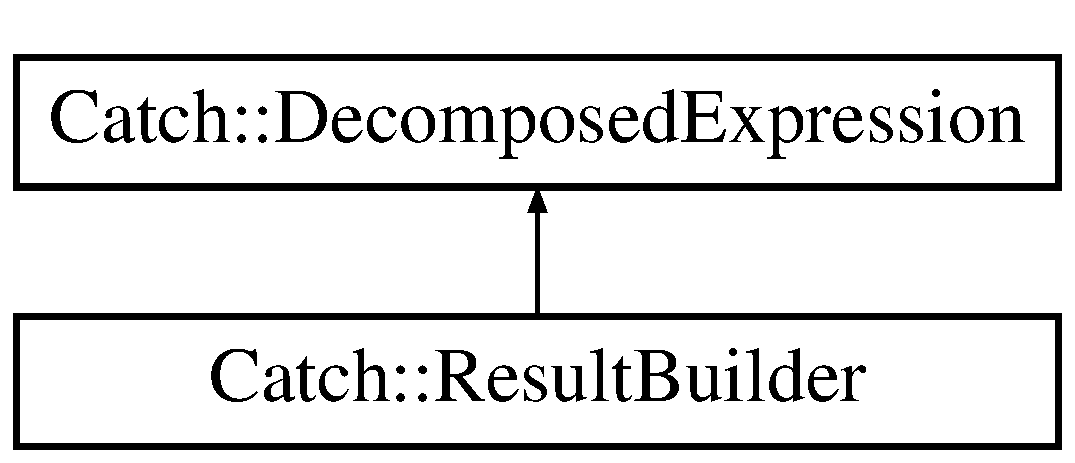
\includegraphics[height=2.000000cm]{class_catch_1_1_result_builder}
\end{center}
\end{figure}
\subsection*{Public Member Functions}
\begin{DoxyCompactItemize}
\item 
\mbox{\hyperlink{class_catch_1_1_result_builder_a8579c3056f64f9324cf1181532828376}{Result\+Builder}} (char const $\ast$macro\+Name, \mbox{\hyperlink{struct_catch_1_1_source_line_info}{Source\+Line\+Info}} const \&line\+Info, char const $\ast$captured\+Expression, \mbox{\hyperlink{struct_catch_1_1_result_disposition_a3396cad6e2259af326b3aae93e23e9d8}{Result\+Disposition\+::\+Flags}} result\+Disposition, char const $\ast$second\+Arg=\char`\"{}\char`\"{})
\item 
\mbox{\hyperlink{class_catch_1_1_result_builder_a687d1e9521d97f93c883ab070cc94c64}{$\sim$\+Result\+Builder}} ()
\item 
{\footnotesize template$<$typename T $>$ }\\\mbox{\hyperlink{class_catch_1_1_expression_lhs}{Expression\+Lhs}}$<$ T const  \& $>$ \mbox{\hyperlink{class_catch_1_1_result_builder_ad76939f5a52fcb534f97b49a0b7bc560}{operator$<$=}} (T const \&operand)
\item 
\mbox{\hyperlink{class_catch_1_1_expression_lhs}{Expression\+Lhs}}$<$ bool $>$ \mbox{\hyperlink{class_catch_1_1_result_builder_a3b87b20bcd1ef9e630880e59eeefba2a}{operator$<$=}} (bool value)
\item 
{\footnotesize template$<$typename T $>$ }\\\mbox{\hyperlink{class_catch_1_1_result_builder}{Result\+Builder}} \& \mbox{\hyperlink{class_catch_1_1_result_builder_a5aa79ce6160ab8cd800eb65bbd7a28a4}{operator$<$$<$}} (T const \&value)
\item 
\mbox{\hyperlink{class_catch_1_1_result_builder}{Result\+Builder}} \& \mbox{\hyperlink{class_catch_1_1_result_builder_af896e372db9d7fc90ddeceff3ad110d0}{set\+Result\+Type}} (\mbox{\hyperlink{struct_catch_1_1_result_was_a624e1ee3661fcf6094ceef1f654601ef}{Result\+Was\+::\+Of\+Type}} result)
\item 
\mbox{\hyperlink{class_catch_1_1_result_builder}{Result\+Builder}} \& \mbox{\hyperlink{class_catch_1_1_result_builder_ae504348b073d0360bfd5fc33347ec689}{set\+Result\+Type}} (bool result)
\item 
void \mbox{\hyperlink{class_catch_1_1_result_builder_a864e03b7300271de7cc44b9864463c5a}{end\+Expression}} (\mbox{\hyperlink{struct_catch_1_1_decomposed_expression}{Decomposed\+Expression}} const \&expr)
\item 
virtual void \mbox{\hyperlink{class_catch_1_1_result_builder_a7d94b15cf04301a8617e7b16158b5d82}{reconstruct\+Expression}} (std\+::string \&dest) const \mbox{\hyperlink{catch_8hpp_a8ecdce4d3f57835f707915ae831eb847}{C\+A\+T\+C\+H\+\_\+\+O\+V\+E\+R\+R\+I\+DE}}
\item 
\mbox{\hyperlink{class_catch_1_1_assertion_result}{Assertion\+Result}} \mbox{\hyperlink{class_catch_1_1_result_builder_a4fc96e7bb8b5f7119a8e79692ec97808}{build}} () const
\item 
\mbox{\hyperlink{class_catch_1_1_assertion_result}{Assertion\+Result}} \mbox{\hyperlink{class_catch_1_1_result_builder_a475d19a04c5d10a5a87cbb85447b59da}{build}} (\mbox{\hyperlink{struct_catch_1_1_decomposed_expression}{Decomposed\+Expression}} const \&expr) const
\item 
void \mbox{\hyperlink{class_catch_1_1_result_builder_a5bbd2f14a678f3e8d0f791ac6d233d65}{use\+Active\+Exception}} (\mbox{\hyperlink{struct_catch_1_1_result_disposition_a3396cad6e2259af326b3aae93e23e9d8}{Result\+Disposition\+::\+Flags}} result\+Disposition=\mbox{\hyperlink{struct_catch_1_1_result_disposition_a3396cad6e2259af326b3aae93e23e9d8af3bd52347ed6f8796e8ce2f77bb39ea5}{Result\+Disposition\+::\+Normal}})
\item 
void \mbox{\hyperlink{class_catch_1_1_result_builder_a10e467f7b7a4976e5d148b4d5066e8fd}{capture\+Result}} (\mbox{\hyperlink{struct_catch_1_1_result_was_a624e1ee3661fcf6094ceef1f654601ef}{Result\+Was\+::\+Of\+Type}} result\+Type)
\item 
void \mbox{\hyperlink{class_catch_1_1_result_builder_af2ae2343965802eeeb0abbd4ea9d2d36}{capture\+Expression}} ()
\item 
void \mbox{\hyperlink{class_catch_1_1_result_builder_a9ac96f6220c8dd8e4feee725c6228d77}{capture\+Expected\+Exception}} (std\+::string const \&expected\+Message)
\item 
void \mbox{\hyperlink{class_catch_1_1_result_builder_a2d6a194258f07f212fef098c0201038a}{capture\+Expected\+Exception}} (\mbox{\hyperlink{struct_catch_1_1_matchers_1_1_impl_1_1_matcher_base}{Matchers\+::\+Impl\+::\+Matcher\+Base}}$<$ std\+::string $>$ const \&matcher)
\item 
void \mbox{\hyperlink{class_catch_1_1_result_builder_ad8bb17e4ac590b75bf8630d8f3502f4e}{handle\+Result}} (\mbox{\hyperlink{class_catch_1_1_assertion_result}{Assertion\+Result}} const \&result)
\item 
void \mbox{\hyperlink{class_catch_1_1_result_builder_a3085cdc46533d45bed6f652a2ac295c0}{react}} ()
\item 
bool \mbox{\hyperlink{class_catch_1_1_result_builder_a6f2b0dbcc6cc5e0a500ac45f2534e3e7}{should\+Debug\+Break}} () const
\item 
bool \mbox{\hyperlink{class_catch_1_1_result_builder_a0428fd78ab9e8e6f1aca6855f20fc715}{allow\+Throws}} () const
\item 
{\footnotesize template$<$typename ArgT , typename MatcherT $>$ }\\void \mbox{\hyperlink{class_catch_1_1_result_builder_a27425538bec8fee7ac69403c5df6078c}{capture\+Match}} (ArgT const \&arg, MatcherT const \&matcher, char const $\ast$matcher\+String)
\item 
void \mbox{\hyperlink{class_catch_1_1_result_builder_a87929808b4ec9b6cb5838edc1f27df17}{set\+Exception\+Guard}} ()
\item 
void \mbox{\hyperlink{class_catch_1_1_result_builder_a0990e93c1e13f96ffe02fa0f45e8f155}{unset\+Exception\+Guard}} ()
\end{DoxyCompactItemize}


\subsection{Constructor \& Destructor Documentation}
\mbox{\Hypertarget{class_catch_1_1_result_builder_a8579c3056f64f9324cf1181532828376}\label{class_catch_1_1_result_builder_a8579c3056f64f9324cf1181532828376}} 
\index{Catch\+::\+Result\+Builder@{Catch\+::\+Result\+Builder}!Result\+Builder@{Result\+Builder}}
\index{Result\+Builder@{Result\+Builder}!Catch\+::\+Result\+Builder@{Catch\+::\+Result\+Builder}}
\subsubsection{\texorpdfstring{Result\+Builder()}{ResultBuilder()}}
{\footnotesize\ttfamily Catch\+::\+Result\+Builder\+::\+Result\+Builder (\begin{DoxyParamCaption}\item[{char const $\ast$}]{macro\+Name,  }\item[{\mbox{\hyperlink{struct_catch_1_1_source_line_info}{Source\+Line\+Info}} const \&}]{line\+Info,  }\item[{char const $\ast$}]{captured\+Expression,  }\item[{\mbox{\hyperlink{struct_catch_1_1_result_disposition_a3396cad6e2259af326b3aae93e23e9d8}{Result\+Disposition\+::\+Flags}}}]{result\+Disposition,  }\item[{char const $\ast$}]{second\+Arg = {\ttfamily \char`\"{}\char`\"{}} }\end{DoxyParamCaption})}

\mbox{\Hypertarget{class_catch_1_1_result_builder_a687d1e9521d97f93c883ab070cc94c64}\label{class_catch_1_1_result_builder_a687d1e9521d97f93c883ab070cc94c64}} 
\index{Catch\+::\+Result\+Builder@{Catch\+::\+Result\+Builder}!````~Result\+Builder@{$\sim$\+Result\+Builder}}
\index{````~Result\+Builder@{$\sim$\+Result\+Builder}!Catch\+::\+Result\+Builder@{Catch\+::\+Result\+Builder}}
\subsubsection{\texorpdfstring{$\sim$\+Result\+Builder()}{~ResultBuilder()}}
{\footnotesize\ttfamily Catch\+::\+Result\+Builder\+::$\sim$\+Result\+Builder (\begin{DoxyParamCaption}{ }\end{DoxyParamCaption})}



\subsection{Member Function Documentation}
\mbox{\Hypertarget{class_catch_1_1_result_builder_a0428fd78ab9e8e6f1aca6855f20fc715}\label{class_catch_1_1_result_builder_a0428fd78ab9e8e6f1aca6855f20fc715}} 
\index{Catch\+::\+Result\+Builder@{Catch\+::\+Result\+Builder}!allow\+Throws@{allow\+Throws}}
\index{allow\+Throws@{allow\+Throws}!Catch\+::\+Result\+Builder@{Catch\+::\+Result\+Builder}}
\subsubsection{\texorpdfstring{allow\+Throws()}{allowThrows()}}
{\footnotesize\ttfamily bool Catch\+::\+Result\+Builder\+::allow\+Throws (\begin{DoxyParamCaption}{ }\end{DoxyParamCaption}) const}

\mbox{\Hypertarget{class_catch_1_1_result_builder_a4fc96e7bb8b5f7119a8e79692ec97808}\label{class_catch_1_1_result_builder_a4fc96e7bb8b5f7119a8e79692ec97808}} 
\index{Catch\+::\+Result\+Builder@{Catch\+::\+Result\+Builder}!build@{build}}
\index{build@{build}!Catch\+::\+Result\+Builder@{Catch\+::\+Result\+Builder}}
\subsubsection{\texorpdfstring{build()}{build()}\hspace{0.1cm}{\footnotesize\ttfamily [1/2]}}
{\footnotesize\ttfamily \mbox{\hyperlink{class_catch_1_1_assertion_result}{Assertion\+Result}} Catch\+::\+Result\+Builder\+::build (\begin{DoxyParamCaption}{ }\end{DoxyParamCaption}) const}

\mbox{\Hypertarget{class_catch_1_1_result_builder_a475d19a04c5d10a5a87cbb85447b59da}\label{class_catch_1_1_result_builder_a475d19a04c5d10a5a87cbb85447b59da}} 
\index{Catch\+::\+Result\+Builder@{Catch\+::\+Result\+Builder}!build@{build}}
\index{build@{build}!Catch\+::\+Result\+Builder@{Catch\+::\+Result\+Builder}}
\subsubsection{\texorpdfstring{build()}{build()}\hspace{0.1cm}{\footnotesize\ttfamily [2/2]}}
{\footnotesize\ttfamily \mbox{\hyperlink{class_catch_1_1_assertion_result}{Assertion\+Result}} Catch\+::\+Result\+Builder\+::build (\begin{DoxyParamCaption}\item[{\mbox{\hyperlink{struct_catch_1_1_decomposed_expression}{Decomposed\+Expression}} const \&}]{expr }\end{DoxyParamCaption}) const}

\mbox{\Hypertarget{class_catch_1_1_result_builder_a9ac96f6220c8dd8e4feee725c6228d77}\label{class_catch_1_1_result_builder_a9ac96f6220c8dd8e4feee725c6228d77}} 
\index{Catch\+::\+Result\+Builder@{Catch\+::\+Result\+Builder}!capture\+Expected\+Exception@{capture\+Expected\+Exception}}
\index{capture\+Expected\+Exception@{capture\+Expected\+Exception}!Catch\+::\+Result\+Builder@{Catch\+::\+Result\+Builder}}
\subsubsection{\texorpdfstring{capture\+Expected\+Exception()}{captureExpectedException()}\hspace{0.1cm}{\footnotesize\ttfamily [1/2]}}
{\footnotesize\ttfamily void Catch\+::\+Result\+Builder\+::capture\+Expected\+Exception (\begin{DoxyParamCaption}\item[{std\+::string const \&}]{expected\+Message }\end{DoxyParamCaption})}

\mbox{\Hypertarget{class_catch_1_1_result_builder_a2d6a194258f07f212fef098c0201038a}\label{class_catch_1_1_result_builder_a2d6a194258f07f212fef098c0201038a}} 
\index{Catch\+::\+Result\+Builder@{Catch\+::\+Result\+Builder}!capture\+Expected\+Exception@{capture\+Expected\+Exception}}
\index{capture\+Expected\+Exception@{capture\+Expected\+Exception}!Catch\+::\+Result\+Builder@{Catch\+::\+Result\+Builder}}
\subsubsection{\texorpdfstring{capture\+Expected\+Exception()}{captureExpectedException()}\hspace{0.1cm}{\footnotesize\ttfamily [2/2]}}
{\footnotesize\ttfamily void Catch\+::\+Result\+Builder\+::capture\+Expected\+Exception (\begin{DoxyParamCaption}\item[{\mbox{\hyperlink{struct_catch_1_1_matchers_1_1_impl_1_1_matcher_base}{Matchers\+::\+Impl\+::\+Matcher\+Base}}$<$ std\+::string $>$ const \&}]{matcher }\end{DoxyParamCaption})}

\mbox{\Hypertarget{class_catch_1_1_result_builder_af2ae2343965802eeeb0abbd4ea9d2d36}\label{class_catch_1_1_result_builder_af2ae2343965802eeeb0abbd4ea9d2d36}} 
\index{Catch\+::\+Result\+Builder@{Catch\+::\+Result\+Builder}!capture\+Expression@{capture\+Expression}}
\index{capture\+Expression@{capture\+Expression}!Catch\+::\+Result\+Builder@{Catch\+::\+Result\+Builder}}
\subsubsection{\texorpdfstring{capture\+Expression()}{captureExpression()}}
{\footnotesize\ttfamily void Catch\+::\+Result\+Builder\+::capture\+Expression (\begin{DoxyParamCaption}{ }\end{DoxyParamCaption})}

\mbox{\Hypertarget{class_catch_1_1_result_builder_a27425538bec8fee7ac69403c5df6078c}\label{class_catch_1_1_result_builder_a27425538bec8fee7ac69403c5df6078c}} 
\index{Catch\+::\+Result\+Builder@{Catch\+::\+Result\+Builder}!capture\+Match@{capture\+Match}}
\index{capture\+Match@{capture\+Match}!Catch\+::\+Result\+Builder@{Catch\+::\+Result\+Builder}}
\subsubsection{\texorpdfstring{capture\+Match()}{captureMatch()}}
{\footnotesize\ttfamily template$<$typename ArgT , typename MatcherT $>$ \\
void Catch\+::\+Result\+Builder\+::capture\+Match (\begin{DoxyParamCaption}\item[{ArgT const \&}]{arg,  }\item[{MatcherT const \&}]{matcher,  }\item[{char const $\ast$}]{matcher\+String }\end{DoxyParamCaption})\hspace{0.3cm}{\ttfamily [inline]}}

\mbox{\Hypertarget{class_catch_1_1_result_builder_a10e467f7b7a4976e5d148b4d5066e8fd}\label{class_catch_1_1_result_builder_a10e467f7b7a4976e5d148b4d5066e8fd}} 
\index{Catch\+::\+Result\+Builder@{Catch\+::\+Result\+Builder}!capture\+Result@{capture\+Result}}
\index{capture\+Result@{capture\+Result}!Catch\+::\+Result\+Builder@{Catch\+::\+Result\+Builder}}
\subsubsection{\texorpdfstring{capture\+Result()}{captureResult()}}
{\footnotesize\ttfamily void Catch\+::\+Result\+Builder\+::capture\+Result (\begin{DoxyParamCaption}\item[{\mbox{\hyperlink{struct_catch_1_1_result_was_a624e1ee3661fcf6094ceef1f654601ef}{Result\+Was\+::\+Of\+Type}}}]{result\+Type }\end{DoxyParamCaption})}

\mbox{\Hypertarget{class_catch_1_1_result_builder_a864e03b7300271de7cc44b9864463c5a}\label{class_catch_1_1_result_builder_a864e03b7300271de7cc44b9864463c5a}} 
\index{Catch\+::\+Result\+Builder@{Catch\+::\+Result\+Builder}!end\+Expression@{end\+Expression}}
\index{end\+Expression@{end\+Expression}!Catch\+::\+Result\+Builder@{Catch\+::\+Result\+Builder}}
\subsubsection{\texorpdfstring{end\+Expression()}{endExpression()}}
{\footnotesize\ttfamily void Catch\+::\+Result\+Builder\+::end\+Expression (\begin{DoxyParamCaption}\item[{\mbox{\hyperlink{struct_catch_1_1_decomposed_expression}{Decomposed\+Expression}} const \&}]{expr }\end{DoxyParamCaption})}

\mbox{\Hypertarget{class_catch_1_1_result_builder_ad8bb17e4ac590b75bf8630d8f3502f4e}\label{class_catch_1_1_result_builder_ad8bb17e4ac590b75bf8630d8f3502f4e}} 
\index{Catch\+::\+Result\+Builder@{Catch\+::\+Result\+Builder}!handle\+Result@{handle\+Result}}
\index{handle\+Result@{handle\+Result}!Catch\+::\+Result\+Builder@{Catch\+::\+Result\+Builder}}
\subsubsection{\texorpdfstring{handle\+Result()}{handleResult()}}
{\footnotesize\ttfamily void Catch\+::\+Result\+Builder\+::handle\+Result (\begin{DoxyParamCaption}\item[{\mbox{\hyperlink{class_catch_1_1_assertion_result}{Assertion\+Result}} const \&}]{result }\end{DoxyParamCaption})}

\mbox{\Hypertarget{class_catch_1_1_result_builder_a5aa79ce6160ab8cd800eb65bbd7a28a4}\label{class_catch_1_1_result_builder_a5aa79ce6160ab8cd800eb65bbd7a28a4}} 
\index{Catch\+::\+Result\+Builder@{Catch\+::\+Result\+Builder}!operator$<$$<$@{operator$<$$<$}}
\index{operator$<$$<$@{operator$<$$<$}!Catch\+::\+Result\+Builder@{Catch\+::\+Result\+Builder}}
\subsubsection{\texorpdfstring{operator$<$$<$()}{operator<<()}}
{\footnotesize\ttfamily template$<$typename T $>$ \\
\mbox{\hyperlink{class_catch_1_1_result_builder}{Result\+Builder}}\& Catch\+::\+Result\+Builder\+::operator$<$$<$ (\begin{DoxyParamCaption}\item[{T const \&}]{value }\end{DoxyParamCaption})\hspace{0.3cm}{\ttfamily [inline]}}

\mbox{\Hypertarget{class_catch_1_1_result_builder_a3b87b20bcd1ef9e630880e59eeefba2a}\label{class_catch_1_1_result_builder_a3b87b20bcd1ef9e630880e59eeefba2a}} 
\index{Catch\+::\+Result\+Builder@{Catch\+::\+Result\+Builder}!operator$<$=@{operator$<$=}}
\index{operator$<$=@{operator$<$=}!Catch\+::\+Result\+Builder@{Catch\+::\+Result\+Builder}}
\subsubsection{\texorpdfstring{operator$<$=()}{operator<=()}\hspace{0.1cm}{\footnotesize\ttfamily [1/2]}}
{\footnotesize\ttfamily \mbox{\hyperlink{class_catch_1_1_expression_lhs}{Expression\+Lhs}}$<$ bool $>$ Catch\+::\+Result\+Builder\+::operator$<$= (\begin{DoxyParamCaption}\item[{bool}]{value }\end{DoxyParamCaption})\hspace{0.3cm}{\ttfamily [inline]}}

\mbox{\Hypertarget{class_catch_1_1_result_builder_ad76939f5a52fcb534f97b49a0b7bc560}\label{class_catch_1_1_result_builder_ad76939f5a52fcb534f97b49a0b7bc560}} 
\index{Catch\+::\+Result\+Builder@{Catch\+::\+Result\+Builder}!operator$<$=@{operator$<$=}}
\index{operator$<$=@{operator$<$=}!Catch\+::\+Result\+Builder@{Catch\+::\+Result\+Builder}}
\subsubsection{\texorpdfstring{operator$<$=()}{operator<=()}\hspace{0.1cm}{\footnotesize\ttfamily [2/2]}}
{\footnotesize\ttfamily template$<$typename T $>$ \\
\mbox{\hyperlink{class_catch_1_1_expression_lhs}{Expression\+Lhs}}$<$ T const  \& $>$ Catch\+::\+Result\+Builder\+::operator$<$= (\begin{DoxyParamCaption}\item[{T const \&}]{operand }\end{DoxyParamCaption})\hspace{0.3cm}{\ttfamily [inline]}}

\mbox{\Hypertarget{class_catch_1_1_result_builder_a3085cdc46533d45bed6f652a2ac295c0}\label{class_catch_1_1_result_builder_a3085cdc46533d45bed6f652a2ac295c0}} 
\index{Catch\+::\+Result\+Builder@{Catch\+::\+Result\+Builder}!react@{react}}
\index{react@{react}!Catch\+::\+Result\+Builder@{Catch\+::\+Result\+Builder}}
\subsubsection{\texorpdfstring{react()}{react()}}
{\footnotesize\ttfamily void Catch\+::\+Result\+Builder\+::react (\begin{DoxyParamCaption}{ }\end{DoxyParamCaption})}

\mbox{\Hypertarget{class_catch_1_1_result_builder_a7d94b15cf04301a8617e7b16158b5d82}\label{class_catch_1_1_result_builder_a7d94b15cf04301a8617e7b16158b5d82}} 
\index{Catch\+::\+Result\+Builder@{Catch\+::\+Result\+Builder}!reconstruct\+Expression@{reconstruct\+Expression}}
\index{reconstruct\+Expression@{reconstruct\+Expression}!Catch\+::\+Result\+Builder@{Catch\+::\+Result\+Builder}}
\subsubsection{\texorpdfstring{reconstruct\+Expression()}{reconstructExpression()}}
{\footnotesize\ttfamily virtual void Catch\+::\+Result\+Builder\+::reconstruct\+Expression (\begin{DoxyParamCaption}\item[{std\+::string \&}]{dest }\end{DoxyParamCaption}) const\hspace{0.3cm}{\ttfamily [virtual]}}



Implements \mbox{\hyperlink{struct_catch_1_1_decomposed_expression_a9ce7f356dc96f11f80e40c82f5aa7e55}{Catch\+::\+Decomposed\+Expression}}.

\mbox{\Hypertarget{class_catch_1_1_result_builder_a87929808b4ec9b6cb5838edc1f27df17}\label{class_catch_1_1_result_builder_a87929808b4ec9b6cb5838edc1f27df17}} 
\index{Catch\+::\+Result\+Builder@{Catch\+::\+Result\+Builder}!set\+Exception\+Guard@{set\+Exception\+Guard}}
\index{set\+Exception\+Guard@{set\+Exception\+Guard}!Catch\+::\+Result\+Builder@{Catch\+::\+Result\+Builder}}
\subsubsection{\texorpdfstring{set\+Exception\+Guard()}{setExceptionGuard()}}
{\footnotesize\ttfamily void Catch\+::\+Result\+Builder\+::set\+Exception\+Guard (\begin{DoxyParamCaption}{ }\end{DoxyParamCaption})}

\mbox{\Hypertarget{class_catch_1_1_result_builder_af896e372db9d7fc90ddeceff3ad110d0}\label{class_catch_1_1_result_builder_af896e372db9d7fc90ddeceff3ad110d0}} 
\index{Catch\+::\+Result\+Builder@{Catch\+::\+Result\+Builder}!set\+Result\+Type@{set\+Result\+Type}}
\index{set\+Result\+Type@{set\+Result\+Type}!Catch\+::\+Result\+Builder@{Catch\+::\+Result\+Builder}}
\subsubsection{\texorpdfstring{set\+Result\+Type()}{setResultType()}\hspace{0.1cm}{\footnotesize\ttfamily [1/2]}}
{\footnotesize\ttfamily \mbox{\hyperlink{class_catch_1_1_result_builder}{Result\+Builder}}\& Catch\+::\+Result\+Builder\+::set\+Result\+Type (\begin{DoxyParamCaption}\item[{\mbox{\hyperlink{struct_catch_1_1_result_was_a624e1ee3661fcf6094ceef1f654601ef}{Result\+Was\+::\+Of\+Type}}}]{result }\end{DoxyParamCaption})}

\mbox{\Hypertarget{class_catch_1_1_result_builder_ae504348b073d0360bfd5fc33347ec689}\label{class_catch_1_1_result_builder_ae504348b073d0360bfd5fc33347ec689}} 
\index{Catch\+::\+Result\+Builder@{Catch\+::\+Result\+Builder}!set\+Result\+Type@{set\+Result\+Type}}
\index{set\+Result\+Type@{set\+Result\+Type}!Catch\+::\+Result\+Builder@{Catch\+::\+Result\+Builder}}
\subsubsection{\texorpdfstring{set\+Result\+Type()}{setResultType()}\hspace{0.1cm}{\footnotesize\ttfamily [2/2]}}
{\footnotesize\ttfamily \mbox{\hyperlink{class_catch_1_1_result_builder}{Result\+Builder}}\& Catch\+::\+Result\+Builder\+::set\+Result\+Type (\begin{DoxyParamCaption}\item[{bool}]{result }\end{DoxyParamCaption})}

\mbox{\Hypertarget{class_catch_1_1_result_builder_a6f2b0dbcc6cc5e0a500ac45f2534e3e7}\label{class_catch_1_1_result_builder_a6f2b0dbcc6cc5e0a500ac45f2534e3e7}} 
\index{Catch\+::\+Result\+Builder@{Catch\+::\+Result\+Builder}!should\+Debug\+Break@{should\+Debug\+Break}}
\index{should\+Debug\+Break@{should\+Debug\+Break}!Catch\+::\+Result\+Builder@{Catch\+::\+Result\+Builder}}
\subsubsection{\texorpdfstring{should\+Debug\+Break()}{shouldDebugBreak()}}
{\footnotesize\ttfamily bool Catch\+::\+Result\+Builder\+::should\+Debug\+Break (\begin{DoxyParamCaption}{ }\end{DoxyParamCaption}) const}

\mbox{\Hypertarget{class_catch_1_1_result_builder_a0990e93c1e13f96ffe02fa0f45e8f155}\label{class_catch_1_1_result_builder_a0990e93c1e13f96ffe02fa0f45e8f155}} 
\index{Catch\+::\+Result\+Builder@{Catch\+::\+Result\+Builder}!unset\+Exception\+Guard@{unset\+Exception\+Guard}}
\index{unset\+Exception\+Guard@{unset\+Exception\+Guard}!Catch\+::\+Result\+Builder@{Catch\+::\+Result\+Builder}}
\subsubsection{\texorpdfstring{unset\+Exception\+Guard()}{unsetExceptionGuard()}}
{\footnotesize\ttfamily void Catch\+::\+Result\+Builder\+::unset\+Exception\+Guard (\begin{DoxyParamCaption}{ }\end{DoxyParamCaption})}

\mbox{\Hypertarget{class_catch_1_1_result_builder_a5bbd2f14a678f3e8d0f791ac6d233d65}\label{class_catch_1_1_result_builder_a5bbd2f14a678f3e8d0f791ac6d233d65}} 
\index{Catch\+::\+Result\+Builder@{Catch\+::\+Result\+Builder}!use\+Active\+Exception@{use\+Active\+Exception}}
\index{use\+Active\+Exception@{use\+Active\+Exception}!Catch\+::\+Result\+Builder@{Catch\+::\+Result\+Builder}}
\subsubsection{\texorpdfstring{use\+Active\+Exception()}{useActiveException()}}
{\footnotesize\ttfamily void Catch\+::\+Result\+Builder\+::use\+Active\+Exception (\begin{DoxyParamCaption}\item[{\mbox{\hyperlink{struct_catch_1_1_result_disposition_a3396cad6e2259af326b3aae93e23e9d8}{Result\+Disposition\+::\+Flags}}}]{result\+Disposition = {\ttfamily \mbox{\hyperlink{struct_catch_1_1_result_disposition_a3396cad6e2259af326b3aae93e23e9d8af3bd52347ed6f8796e8ce2f77bb39ea5}{Result\+Disposition\+::\+Normal}}} }\end{DoxyParamCaption})}



The documentation for this class was generated from the following file\+:\begin{DoxyCompactItemize}
\item 
include/\mbox{\hyperlink{catch_8hpp}{catch.\+hpp}}\end{DoxyCompactItemize}

\hypertarget{struct_catch_1_1_result_disposition}{}\section{Catch\+:\+:Result\+Disposition Struct Reference}
\label{struct_catch_1_1_result_disposition}\index{Catch\+::\+Result\+Disposition@{Catch\+::\+Result\+Disposition}}


{\ttfamily \#include $<$catch.\+hpp$>$}

\subsection*{Public Types}
\begin{DoxyCompactItemize}
\item 
enum \mbox{\hyperlink{struct_catch_1_1_result_disposition_a3396cad6e2259af326b3aae93e23e9d8}{Flags}} \{ \mbox{\hyperlink{struct_catch_1_1_result_disposition_a3396cad6e2259af326b3aae93e23e9d8af3bd52347ed6f8796e8ce2f77bb39ea5}{Normal}} = 0x01, 
\mbox{\hyperlink{struct_catch_1_1_result_disposition_a3396cad6e2259af326b3aae93e23e9d8aa18c94bd60c5614e17a84c2ced3bbfd5}{Continue\+On\+Failure}} = 0x02, 
\mbox{\hyperlink{struct_catch_1_1_result_disposition_a3396cad6e2259af326b3aae93e23e9d8a9980604245f19884691f941dec03eeb8}{False\+Test}} = 0x04, 
\mbox{\hyperlink{struct_catch_1_1_result_disposition_a3396cad6e2259af326b3aae93e23e9d8a1a88eb6004bddee4ccae4b421991bf54}{Suppress\+Fail}} = 0x08
 \}
\end{DoxyCompactItemize}


\subsection{Member Enumeration Documentation}
\mbox{\Hypertarget{struct_catch_1_1_result_disposition_a3396cad6e2259af326b3aae93e23e9d8}\label{struct_catch_1_1_result_disposition_a3396cad6e2259af326b3aae93e23e9d8}} 
\index{Catch\+::\+Result\+Disposition@{Catch\+::\+Result\+Disposition}!Flags@{Flags}}
\index{Flags@{Flags}!Catch\+::\+Result\+Disposition@{Catch\+::\+Result\+Disposition}}
\subsubsection{\texorpdfstring{Flags}{Flags}}
{\footnotesize\ttfamily enum \mbox{\hyperlink{struct_catch_1_1_result_disposition_a3396cad6e2259af326b3aae93e23e9d8}{Catch\+::\+Result\+Disposition\+::\+Flags}}}

\begin{DoxyEnumFields}{Enumerator}
\raisebox{\heightof{T}}[0pt][0pt]{\index{Normal@{Normal}!Catch\+::\+Result\+Disposition@{Catch\+::\+Result\+Disposition}}\index{Catch\+::\+Result\+Disposition@{Catch\+::\+Result\+Disposition}!Normal@{Normal}}}\mbox{\Hypertarget{struct_catch_1_1_result_disposition_a3396cad6e2259af326b3aae93e23e9d8af3bd52347ed6f8796e8ce2f77bb39ea5}\label{struct_catch_1_1_result_disposition_a3396cad6e2259af326b3aae93e23e9d8af3bd52347ed6f8796e8ce2f77bb39ea5}} 
Normal&\\
\hline

\raisebox{\heightof{T}}[0pt][0pt]{\index{Continue\+On\+Failure@{Continue\+On\+Failure}!Catch\+::\+Result\+Disposition@{Catch\+::\+Result\+Disposition}}\index{Catch\+::\+Result\+Disposition@{Catch\+::\+Result\+Disposition}!Continue\+On\+Failure@{Continue\+On\+Failure}}}\mbox{\Hypertarget{struct_catch_1_1_result_disposition_a3396cad6e2259af326b3aae93e23e9d8aa18c94bd60c5614e17a84c2ced3bbfd5}\label{struct_catch_1_1_result_disposition_a3396cad6e2259af326b3aae93e23e9d8aa18c94bd60c5614e17a84c2ced3bbfd5}} 
Continue\+On\+Failure&\\
\hline

\raisebox{\heightof{T}}[0pt][0pt]{\index{False\+Test@{False\+Test}!Catch\+::\+Result\+Disposition@{Catch\+::\+Result\+Disposition}}\index{Catch\+::\+Result\+Disposition@{Catch\+::\+Result\+Disposition}!False\+Test@{False\+Test}}}\mbox{\Hypertarget{struct_catch_1_1_result_disposition_a3396cad6e2259af326b3aae93e23e9d8a9980604245f19884691f941dec03eeb8}\label{struct_catch_1_1_result_disposition_a3396cad6e2259af326b3aae93e23e9d8a9980604245f19884691f941dec03eeb8}} 
False\+Test&\\
\hline

\raisebox{\heightof{T}}[0pt][0pt]{\index{Suppress\+Fail@{Suppress\+Fail}!Catch\+::\+Result\+Disposition@{Catch\+::\+Result\+Disposition}}\index{Catch\+::\+Result\+Disposition@{Catch\+::\+Result\+Disposition}!Suppress\+Fail@{Suppress\+Fail}}}\mbox{\Hypertarget{struct_catch_1_1_result_disposition_a3396cad6e2259af326b3aae93e23e9d8a1a88eb6004bddee4ccae4b421991bf54}\label{struct_catch_1_1_result_disposition_a3396cad6e2259af326b3aae93e23e9d8a1a88eb6004bddee4ccae4b421991bf54}} 
Suppress\+Fail&\\
\hline

\end{DoxyEnumFields}


The documentation for this struct was generated from the following file\+:\begin{DoxyCompactItemize}
\item 
include/\mbox{\hyperlink{catch_8hpp}{catch.\+hpp}}\end{DoxyCompactItemize}

\hypertarget{struct_catch_1_1_result_was}{}\section{Catch\+:\+:Result\+Was Struct Reference}
\label{struct_catch_1_1_result_was}\index{Catch\+::\+Result\+Was@{Catch\+::\+Result\+Was}}


{\ttfamily \#include $<$catch.\+hpp$>$}

\subsection*{Public Types}
\begin{DoxyCompactItemize}
\item 
enum \mbox{\hyperlink{struct_catch_1_1_result_was_a624e1ee3661fcf6094ceef1f654601ef}{Of\+Type}} \{ \newline
\mbox{\hyperlink{struct_catch_1_1_result_was_a624e1ee3661fcf6094ceef1f654601efa65721dda02fe5efb522e7449e496608a}{Unknown}} = -\/1, 
\mbox{\hyperlink{struct_catch_1_1_result_was_a624e1ee3661fcf6094ceef1f654601efae7cbe89bb9ec7ece9b44d48b63d01b63}{Ok}} = 0, 
\mbox{\hyperlink{struct_catch_1_1_result_was_a624e1ee3661fcf6094ceef1f654601efa30222063929ca1b6318faa78e8242f1c}{Info}} = 1, 
\mbox{\hyperlink{struct_catch_1_1_result_was_a624e1ee3661fcf6094ceef1f654601efa67e9d36ba0f04a60a19896834d840c21}{Warning}} = 2, 
\newline
\mbox{\hyperlink{struct_catch_1_1_result_was_a624e1ee3661fcf6094ceef1f654601efa1818f1b198f10b5734c405142b22025c}{Failure\+Bit}} = 0x10, 
\mbox{\hyperlink{struct_catch_1_1_result_was_a624e1ee3661fcf6094ceef1f654601efa5e7126b8458dc1376ac870a719f7873f}{Expression\+Failed}} = Failure\+Bit $\vert$ 1, 
\mbox{\hyperlink{struct_catch_1_1_result_was_a624e1ee3661fcf6094ceef1f654601efacecfc052e2499499b13304249303cc36}{Explicit\+Failure}} = Failure\+Bit $\vert$ 2, 
\mbox{\hyperlink{struct_catch_1_1_result_was_a624e1ee3661fcf6094ceef1f654601efaa9107b7836cc7590ca668002f76d27c7}{Exception}} = 0x100 $\vert$ Failure\+Bit, 
\newline
\mbox{\hyperlink{struct_catch_1_1_result_was_a624e1ee3661fcf6094ceef1f654601efa3bb56296483947280cf7fa1ad074ab45}{Threw\+Exception}} = Exception $\vert$ 1, 
\mbox{\hyperlink{struct_catch_1_1_result_was_a624e1ee3661fcf6094ceef1f654601efa8b6d3d5bc78d4e7a95543b6ecfbdb57d}{Didnt\+Throw\+Exception}} = Exception $\vert$ 2, 
\mbox{\hyperlink{struct_catch_1_1_result_was_a624e1ee3661fcf6094ceef1f654601efa87fa1f2a2a63290b61948002e2935377}{Fatal\+Error\+Condition}} = 0x200 $\vert$ Failure\+Bit
 \}
\end{DoxyCompactItemize}


\subsection{Member Enumeration Documentation}
\mbox{\Hypertarget{struct_catch_1_1_result_was_a624e1ee3661fcf6094ceef1f654601ef}\label{struct_catch_1_1_result_was_a624e1ee3661fcf6094ceef1f654601ef}} 
\index{Catch\+::\+Result\+Was@{Catch\+::\+Result\+Was}!Of\+Type@{Of\+Type}}
\index{Of\+Type@{Of\+Type}!Catch\+::\+Result\+Was@{Catch\+::\+Result\+Was}}
\subsubsection{\texorpdfstring{Of\+Type}{OfType}}
{\footnotesize\ttfamily enum \mbox{\hyperlink{struct_catch_1_1_result_was_a624e1ee3661fcf6094ceef1f654601ef}{Catch\+::\+Result\+Was\+::\+Of\+Type}}}

\begin{DoxyEnumFields}{Enumerator}
\raisebox{\heightof{T}}[0pt][0pt]{\index{Unknown@{Unknown}!Catch\+::\+Result\+Was@{Catch\+::\+Result\+Was}}\index{Catch\+::\+Result\+Was@{Catch\+::\+Result\+Was}!Unknown@{Unknown}}}\mbox{\Hypertarget{struct_catch_1_1_result_was_a624e1ee3661fcf6094ceef1f654601efa65721dda02fe5efb522e7449e496608a}\label{struct_catch_1_1_result_was_a624e1ee3661fcf6094ceef1f654601efa65721dda02fe5efb522e7449e496608a}} 
Unknown&\\
\hline

\raisebox{\heightof{T}}[0pt][0pt]{\index{Ok@{Ok}!Catch\+::\+Result\+Was@{Catch\+::\+Result\+Was}}\index{Catch\+::\+Result\+Was@{Catch\+::\+Result\+Was}!Ok@{Ok}}}\mbox{\Hypertarget{struct_catch_1_1_result_was_a624e1ee3661fcf6094ceef1f654601efae7cbe89bb9ec7ece9b44d48b63d01b63}\label{struct_catch_1_1_result_was_a624e1ee3661fcf6094ceef1f654601efae7cbe89bb9ec7ece9b44d48b63d01b63}} 
Ok&\\
\hline

\raisebox{\heightof{T}}[0pt][0pt]{\index{Info@{Info}!Catch\+::\+Result\+Was@{Catch\+::\+Result\+Was}}\index{Catch\+::\+Result\+Was@{Catch\+::\+Result\+Was}!Info@{Info}}}\mbox{\Hypertarget{struct_catch_1_1_result_was_a624e1ee3661fcf6094ceef1f654601efa30222063929ca1b6318faa78e8242f1c}\label{struct_catch_1_1_result_was_a624e1ee3661fcf6094ceef1f654601efa30222063929ca1b6318faa78e8242f1c}} 
Info&\\
\hline

\raisebox{\heightof{T}}[0pt][0pt]{\index{Warning@{Warning}!Catch\+::\+Result\+Was@{Catch\+::\+Result\+Was}}\index{Catch\+::\+Result\+Was@{Catch\+::\+Result\+Was}!Warning@{Warning}}}\mbox{\Hypertarget{struct_catch_1_1_result_was_a624e1ee3661fcf6094ceef1f654601efa67e9d36ba0f04a60a19896834d840c21}\label{struct_catch_1_1_result_was_a624e1ee3661fcf6094ceef1f654601efa67e9d36ba0f04a60a19896834d840c21}} 
Warning&\\
\hline

\raisebox{\heightof{T}}[0pt][0pt]{\index{Failure\+Bit@{Failure\+Bit}!Catch\+::\+Result\+Was@{Catch\+::\+Result\+Was}}\index{Catch\+::\+Result\+Was@{Catch\+::\+Result\+Was}!Failure\+Bit@{Failure\+Bit}}}\mbox{\Hypertarget{struct_catch_1_1_result_was_a624e1ee3661fcf6094ceef1f654601efa1818f1b198f10b5734c405142b22025c}\label{struct_catch_1_1_result_was_a624e1ee3661fcf6094ceef1f654601efa1818f1b198f10b5734c405142b22025c}} 
Failure\+Bit&\\
\hline

\raisebox{\heightof{T}}[0pt][0pt]{\index{Expression\+Failed@{Expression\+Failed}!Catch\+::\+Result\+Was@{Catch\+::\+Result\+Was}}\index{Catch\+::\+Result\+Was@{Catch\+::\+Result\+Was}!Expression\+Failed@{Expression\+Failed}}}\mbox{\Hypertarget{struct_catch_1_1_result_was_a624e1ee3661fcf6094ceef1f654601efa5e7126b8458dc1376ac870a719f7873f}\label{struct_catch_1_1_result_was_a624e1ee3661fcf6094ceef1f654601efa5e7126b8458dc1376ac870a719f7873f}} 
Expression\+Failed&\\
\hline

\raisebox{\heightof{T}}[0pt][0pt]{\index{Explicit\+Failure@{Explicit\+Failure}!Catch\+::\+Result\+Was@{Catch\+::\+Result\+Was}}\index{Catch\+::\+Result\+Was@{Catch\+::\+Result\+Was}!Explicit\+Failure@{Explicit\+Failure}}}\mbox{\Hypertarget{struct_catch_1_1_result_was_a624e1ee3661fcf6094ceef1f654601efacecfc052e2499499b13304249303cc36}\label{struct_catch_1_1_result_was_a624e1ee3661fcf6094ceef1f654601efacecfc052e2499499b13304249303cc36}} 
Explicit\+Failure&\\
\hline

\raisebox{\heightof{T}}[0pt][0pt]{\index{Exception@{Exception}!Catch\+::\+Result\+Was@{Catch\+::\+Result\+Was}}\index{Catch\+::\+Result\+Was@{Catch\+::\+Result\+Was}!Exception@{Exception}}}\mbox{\Hypertarget{struct_catch_1_1_result_was_a624e1ee3661fcf6094ceef1f654601efaa9107b7836cc7590ca668002f76d27c7}\label{struct_catch_1_1_result_was_a624e1ee3661fcf6094ceef1f654601efaa9107b7836cc7590ca668002f76d27c7}} 
Exception&\\
\hline

\raisebox{\heightof{T}}[0pt][0pt]{\index{Threw\+Exception@{Threw\+Exception}!Catch\+::\+Result\+Was@{Catch\+::\+Result\+Was}}\index{Catch\+::\+Result\+Was@{Catch\+::\+Result\+Was}!Threw\+Exception@{Threw\+Exception}}}\mbox{\Hypertarget{struct_catch_1_1_result_was_a624e1ee3661fcf6094ceef1f654601efa3bb56296483947280cf7fa1ad074ab45}\label{struct_catch_1_1_result_was_a624e1ee3661fcf6094ceef1f654601efa3bb56296483947280cf7fa1ad074ab45}} 
Threw\+Exception&\\
\hline

\raisebox{\heightof{T}}[0pt][0pt]{\index{Didnt\+Throw\+Exception@{Didnt\+Throw\+Exception}!Catch\+::\+Result\+Was@{Catch\+::\+Result\+Was}}\index{Catch\+::\+Result\+Was@{Catch\+::\+Result\+Was}!Didnt\+Throw\+Exception@{Didnt\+Throw\+Exception}}}\mbox{\Hypertarget{struct_catch_1_1_result_was_a624e1ee3661fcf6094ceef1f654601efa8b6d3d5bc78d4e7a95543b6ecfbdb57d}\label{struct_catch_1_1_result_was_a624e1ee3661fcf6094ceef1f654601efa8b6d3d5bc78d4e7a95543b6ecfbdb57d}} 
Didnt\+Throw\+Exception&\\
\hline

\raisebox{\heightof{T}}[0pt][0pt]{\index{Fatal\+Error\+Condition@{Fatal\+Error\+Condition}!Catch\+::\+Result\+Was@{Catch\+::\+Result\+Was}}\index{Catch\+::\+Result\+Was@{Catch\+::\+Result\+Was}!Fatal\+Error\+Condition@{Fatal\+Error\+Condition}}}\mbox{\Hypertarget{struct_catch_1_1_result_was_a624e1ee3661fcf6094ceef1f654601efa87fa1f2a2a63290b61948002e2935377}\label{struct_catch_1_1_result_was_a624e1ee3661fcf6094ceef1f654601efa87fa1f2a2a63290b61948002e2935377}} 
Fatal\+Error\+Condition&\\
\hline

\end{DoxyEnumFields}


The documentation for this struct was generated from the following file\+:\begin{DoxyCompactItemize}
\item 
include/\mbox{\hyperlink{catch_8hpp}{catch.\+hpp}}\end{DoxyCompactItemize}

\hypertarget{class_catch_1_1_safe_bool}{}\section{Catch\+:\+:Safe\+Bool Class Reference}
\label{class_catch_1_1_safe_bool}\index{Catch\+::\+Safe\+Bool@{Catch\+::\+Safe\+Bool}}


{\ttfamily \#include $<$catch.\+hpp$>$}

\subsection*{Public Types}
\begin{DoxyCompactItemize}
\item 
typedef void(Safe\+Bool\+::$\ast$ \mbox{\hyperlink{class_catch_1_1_safe_bool_a39eef9baed296299d625a54d54a2a958}{type}}) () const
\end{DoxyCompactItemize}
\subsection*{Static Public Member Functions}
\begin{DoxyCompactItemize}
\item 
static \mbox{\hyperlink{class_catch_1_1_safe_bool_a39eef9baed296299d625a54d54a2a958}{type}} \mbox{\hyperlink{class_catch_1_1_safe_bool_af0ea63d9820f8bf7a8b76377913c4e77}{make\+Safe}} (bool value)
\end{DoxyCompactItemize}


\subsection{Member Typedef Documentation}
\mbox{\Hypertarget{class_catch_1_1_safe_bool_a39eef9baed296299d625a54d54a2a958}\label{class_catch_1_1_safe_bool_a39eef9baed296299d625a54d54a2a958}} 
\index{Catch\+::\+Safe\+Bool@{Catch\+::\+Safe\+Bool}!type@{type}}
\index{type@{type}!Catch\+::\+Safe\+Bool@{Catch\+::\+Safe\+Bool}}
\subsubsection{\texorpdfstring{type}{type}}
{\footnotesize\ttfamily typedef void(Safe\+Bool\+::$\ast$ Catch\+::\+Safe\+Bool\+::type) () const}



\subsection{Member Function Documentation}
\mbox{\Hypertarget{class_catch_1_1_safe_bool_af0ea63d9820f8bf7a8b76377913c4e77}\label{class_catch_1_1_safe_bool_af0ea63d9820f8bf7a8b76377913c4e77}} 
\index{Catch\+::\+Safe\+Bool@{Catch\+::\+Safe\+Bool}!make\+Safe@{make\+Safe}}
\index{make\+Safe@{make\+Safe}!Catch\+::\+Safe\+Bool@{Catch\+::\+Safe\+Bool}}
\subsubsection{\texorpdfstring{make\+Safe()}{makeSafe()}}
{\footnotesize\ttfamily static \mbox{\hyperlink{class_catch_1_1_safe_bool_a39eef9baed296299d625a54d54a2a958}{type}} Catch\+::\+Safe\+Bool\+::make\+Safe (\begin{DoxyParamCaption}\item[{bool}]{value }\end{DoxyParamCaption})\hspace{0.3cm}{\ttfamily [inline]}, {\ttfamily [static]}}



The documentation for this class was generated from the following file\+:\begin{DoxyCompactItemize}
\item 
include/\mbox{\hyperlink{catch_8hpp}{catch.\+hpp}}\end{DoxyCompactItemize}

\hypertarget{class_catch_1_1_scoped_message}{}\section{Catch\+:\+:Scoped\+Message Class Reference}
\label{class_catch_1_1_scoped_message}\index{Catch\+::\+Scoped\+Message@{Catch\+::\+Scoped\+Message}}


{\ttfamily \#include $<$catch.\+hpp$>$}

\subsection*{Public Member Functions}
\begin{DoxyCompactItemize}
\item 
\mbox{\hyperlink{class_catch_1_1_scoped_message_a5cc59f0f2ebe840e6607f83004d49a17}{Scoped\+Message}} (\mbox{\hyperlink{struct_catch_1_1_message_builder}{Message\+Builder}} const \&builder)
\item 
\mbox{\hyperlink{class_catch_1_1_scoped_message_ae03a17fd47220d563d4abc73e7518e29}{Scoped\+Message}} (\mbox{\hyperlink{class_catch_1_1_scoped_message}{Scoped\+Message}} const \&other)
\item 
\mbox{\hyperlink{class_catch_1_1_scoped_message_a43190843f9eeb84a0b42b0bc95fdf93a}{$\sim$\+Scoped\+Message}} ()
\end{DoxyCompactItemize}
\subsection*{Public Attributes}
\begin{DoxyCompactItemize}
\item 
\mbox{\hyperlink{struct_catch_1_1_message_info}{Message\+Info}} \mbox{\hyperlink{class_catch_1_1_scoped_message_ae6e1476f389cc6e1586f033b3747b27b}{m\+\_\+info}}
\end{DoxyCompactItemize}


\subsection{Constructor \& Destructor Documentation}
\mbox{\Hypertarget{class_catch_1_1_scoped_message_a5cc59f0f2ebe840e6607f83004d49a17}\label{class_catch_1_1_scoped_message_a5cc59f0f2ebe840e6607f83004d49a17}} 
\index{Catch\+::\+Scoped\+Message@{Catch\+::\+Scoped\+Message}!Scoped\+Message@{Scoped\+Message}}
\index{Scoped\+Message@{Scoped\+Message}!Catch\+::\+Scoped\+Message@{Catch\+::\+Scoped\+Message}}
\subsubsection{\texorpdfstring{Scoped\+Message()}{ScopedMessage()}\hspace{0.1cm}{\footnotesize\ttfamily [1/2]}}
{\footnotesize\ttfamily Catch\+::\+Scoped\+Message\+::\+Scoped\+Message (\begin{DoxyParamCaption}\item[{\mbox{\hyperlink{struct_catch_1_1_message_builder}{Message\+Builder}} const \&}]{builder }\end{DoxyParamCaption})}

\mbox{\Hypertarget{class_catch_1_1_scoped_message_ae03a17fd47220d563d4abc73e7518e29}\label{class_catch_1_1_scoped_message_ae03a17fd47220d563d4abc73e7518e29}} 
\index{Catch\+::\+Scoped\+Message@{Catch\+::\+Scoped\+Message}!Scoped\+Message@{Scoped\+Message}}
\index{Scoped\+Message@{Scoped\+Message}!Catch\+::\+Scoped\+Message@{Catch\+::\+Scoped\+Message}}
\subsubsection{\texorpdfstring{Scoped\+Message()}{ScopedMessage()}\hspace{0.1cm}{\footnotesize\ttfamily [2/2]}}
{\footnotesize\ttfamily Catch\+::\+Scoped\+Message\+::\+Scoped\+Message (\begin{DoxyParamCaption}\item[{\mbox{\hyperlink{class_catch_1_1_scoped_message}{Scoped\+Message}} const \&}]{other }\end{DoxyParamCaption})}

\mbox{\Hypertarget{class_catch_1_1_scoped_message_a43190843f9eeb84a0b42b0bc95fdf93a}\label{class_catch_1_1_scoped_message_a43190843f9eeb84a0b42b0bc95fdf93a}} 
\index{Catch\+::\+Scoped\+Message@{Catch\+::\+Scoped\+Message}!````~Scoped\+Message@{$\sim$\+Scoped\+Message}}
\index{````~Scoped\+Message@{$\sim$\+Scoped\+Message}!Catch\+::\+Scoped\+Message@{Catch\+::\+Scoped\+Message}}
\subsubsection{\texorpdfstring{$\sim$\+Scoped\+Message()}{~ScopedMessage()}}
{\footnotesize\ttfamily Catch\+::\+Scoped\+Message\+::$\sim$\+Scoped\+Message (\begin{DoxyParamCaption}{ }\end{DoxyParamCaption})}



\subsection{Member Data Documentation}
\mbox{\Hypertarget{class_catch_1_1_scoped_message_ae6e1476f389cc6e1586f033b3747b27b}\label{class_catch_1_1_scoped_message_ae6e1476f389cc6e1586f033b3747b27b}} 
\index{Catch\+::\+Scoped\+Message@{Catch\+::\+Scoped\+Message}!m\+\_\+info@{m\+\_\+info}}
\index{m\+\_\+info@{m\+\_\+info}!Catch\+::\+Scoped\+Message@{Catch\+::\+Scoped\+Message}}
\subsubsection{\texorpdfstring{m\+\_\+info}{m\_info}}
{\footnotesize\ttfamily \mbox{\hyperlink{struct_catch_1_1_message_info}{Message\+Info}} Catch\+::\+Scoped\+Message\+::m\+\_\+info}



The documentation for this class was generated from the following file\+:\begin{DoxyCompactItemize}
\item 
include/\mbox{\hyperlink{catch_8hpp}{catch.\+hpp}}\end{DoxyCompactItemize}

\hypertarget{class_catch_1_1_section}{}\section{Catch\+:\+:Section Class Reference}
\label{class_catch_1_1_section}\index{Catch\+::\+Section@{Catch\+::\+Section}}


{\ttfamily \#include $<$catch.\+hpp$>$}

Inheritance diagram for Catch\+:\+:Section\+:\begin{figure}[H]
\begin{center}
\leavevmode
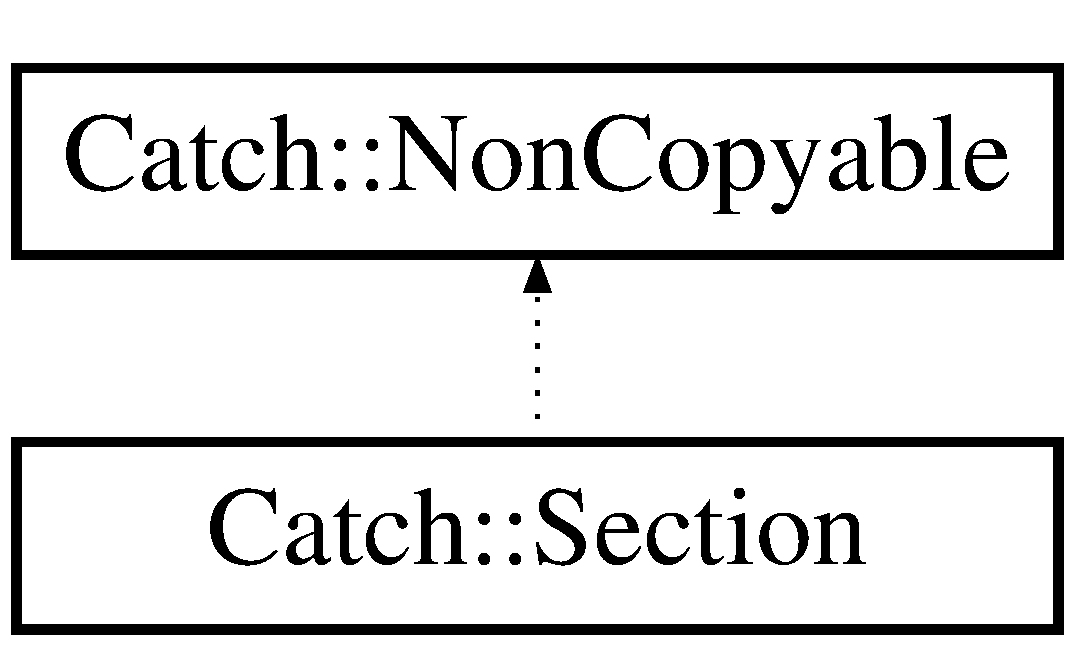
\includegraphics[height=2.000000cm]{class_catch_1_1_section}
\end{center}
\end{figure}
\subsection*{Public Member Functions}
\begin{DoxyCompactItemize}
\item 
\mbox{\hyperlink{class_catch_1_1_section_a68fd4e51e8981aaa7ddb00d8a6abd099}{Section}} (\mbox{\hyperlink{struct_catch_1_1_section_info}{Section\+Info}} const \&info)
\item 
\mbox{\hyperlink{class_catch_1_1_section_aa1422edd68a77aa578b5cc6b8b69f86f}{$\sim$\+Section}} ()
\item 
\mbox{\hyperlink{class_catch_1_1_section_a0632b804dcea1417a2970620a9742eb3}{operator bool}} () const
\end{DoxyCompactItemize}


\subsection{Constructor \& Destructor Documentation}
\mbox{\Hypertarget{class_catch_1_1_section_a68fd4e51e8981aaa7ddb00d8a6abd099}\label{class_catch_1_1_section_a68fd4e51e8981aaa7ddb00d8a6abd099}} 
\index{Catch\+::\+Section@{Catch\+::\+Section}!Section@{Section}}
\index{Section@{Section}!Catch\+::\+Section@{Catch\+::\+Section}}
\subsubsection{\texorpdfstring{Section()}{Section()}}
{\footnotesize\ttfamily Catch\+::\+Section\+::\+Section (\begin{DoxyParamCaption}\item[{\mbox{\hyperlink{struct_catch_1_1_section_info}{Section\+Info}} const \&}]{info }\end{DoxyParamCaption})}

\mbox{\Hypertarget{class_catch_1_1_section_aa1422edd68a77aa578b5cc6b8b69f86f}\label{class_catch_1_1_section_aa1422edd68a77aa578b5cc6b8b69f86f}} 
\index{Catch\+::\+Section@{Catch\+::\+Section}!````~Section@{$\sim$\+Section}}
\index{````~Section@{$\sim$\+Section}!Catch\+::\+Section@{Catch\+::\+Section}}
\subsubsection{\texorpdfstring{$\sim$\+Section()}{~Section()}}
{\footnotesize\ttfamily Catch\+::\+Section\+::$\sim$\+Section (\begin{DoxyParamCaption}{ }\end{DoxyParamCaption})}



\subsection{Member Function Documentation}
\mbox{\Hypertarget{class_catch_1_1_section_a0632b804dcea1417a2970620a9742eb3}\label{class_catch_1_1_section_a0632b804dcea1417a2970620a9742eb3}} 
\index{Catch\+::\+Section@{Catch\+::\+Section}!operator bool@{operator bool}}
\index{operator bool@{operator bool}!Catch\+::\+Section@{Catch\+::\+Section}}
\subsubsection{\texorpdfstring{operator bool()}{operator bool()}}
{\footnotesize\ttfamily Catch\+::\+Section\+::operator bool (\begin{DoxyParamCaption}{ }\end{DoxyParamCaption}) const}



The documentation for this class was generated from the following file\+:\begin{DoxyCompactItemize}
\item 
include/\mbox{\hyperlink{catch_8hpp}{catch.\+hpp}}\end{DoxyCompactItemize}

\hypertarget{struct_catch_1_1_section_end_info}{}\section{Catch\+:\+:Section\+End\+Info Struct Reference}
\label{struct_catch_1_1_section_end_info}\index{Catch\+::\+Section\+End\+Info@{Catch\+::\+Section\+End\+Info}}


{\ttfamily \#include $<$catch.\+hpp$>$}

\subsection*{Public Member Functions}
\begin{DoxyCompactItemize}
\item 
\mbox{\hyperlink{struct_catch_1_1_section_end_info_abc9381c7c22b6907317ec985ccaa6713}{Section\+End\+Info}} (\mbox{\hyperlink{struct_catch_1_1_section_info}{Section\+Info}} const \&\+\_\+section\+Info, \mbox{\hyperlink{struct_catch_1_1_counts}{Counts}} const \&\+\_\+prev\+Assertions, double \+\_\+duration\+In\+Seconds)
\end{DoxyCompactItemize}
\subsection*{Public Attributes}
\begin{DoxyCompactItemize}
\item 
\mbox{\hyperlink{struct_catch_1_1_section_info}{Section\+Info}} \mbox{\hyperlink{struct_catch_1_1_section_end_info_a2d44793392cb83735d086d726822abe9}{section\+Info}}
\item 
\mbox{\hyperlink{struct_catch_1_1_counts}{Counts}} \mbox{\hyperlink{struct_catch_1_1_section_end_info_ae70b154cbc05b5dd2901d97f89303d8c}{prev\+Assertions}}
\item 
double \mbox{\hyperlink{struct_catch_1_1_section_end_info_a7c262f2dab9cff166b8eca620c47eea5}{duration\+In\+Seconds}}
\end{DoxyCompactItemize}


\subsection{Constructor \& Destructor Documentation}
\mbox{\Hypertarget{struct_catch_1_1_section_end_info_abc9381c7c22b6907317ec985ccaa6713}\label{struct_catch_1_1_section_end_info_abc9381c7c22b6907317ec985ccaa6713}} 
\index{Catch\+::\+Section\+End\+Info@{Catch\+::\+Section\+End\+Info}!Section\+End\+Info@{Section\+End\+Info}}
\index{Section\+End\+Info@{Section\+End\+Info}!Catch\+::\+Section\+End\+Info@{Catch\+::\+Section\+End\+Info}}
\subsubsection{\texorpdfstring{Section\+End\+Info()}{SectionEndInfo()}}
{\footnotesize\ttfamily Catch\+::\+Section\+End\+Info\+::\+Section\+End\+Info (\begin{DoxyParamCaption}\item[{\mbox{\hyperlink{struct_catch_1_1_section_info}{Section\+Info}} const \&}]{\+\_\+section\+Info,  }\item[{\mbox{\hyperlink{struct_catch_1_1_counts}{Counts}} const \&}]{\+\_\+prev\+Assertions,  }\item[{double}]{\+\_\+duration\+In\+Seconds }\end{DoxyParamCaption})\hspace{0.3cm}{\ttfamily [inline]}}



\subsection{Member Data Documentation}
\mbox{\Hypertarget{struct_catch_1_1_section_end_info_a7c262f2dab9cff166b8eca620c47eea5}\label{struct_catch_1_1_section_end_info_a7c262f2dab9cff166b8eca620c47eea5}} 
\index{Catch\+::\+Section\+End\+Info@{Catch\+::\+Section\+End\+Info}!duration\+In\+Seconds@{duration\+In\+Seconds}}
\index{duration\+In\+Seconds@{duration\+In\+Seconds}!Catch\+::\+Section\+End\+Info@{Catch\+::\+Section\+End\+Info}}
\subsubsection{\texorpdfstring{duration\+In\+Seconds}{durationInSeconds}}
{\footnotesize\ttfamily double Catch\+::\+Section\+End\+Info\+::duration\+In\+Seconds}

\mbox{\Hypertarget{struct_catch_1_1_section_end_info_ae70b154cbc05b5dd2901d97f89303d8c}\label{struct_catch_1_1_section_end_info_ae70b154cbc05b5dd2901d97f89303d8c}} 
\index{Catch\+::\+Section\+End\+Info@{Catch\+::\+Section\+End\+Info}!prev\+Assertions@{prev\+Assertions}}
\index{prev\+Assertions@{prev\+Assertions}!Catch\+::\+Section\+End\+Info@{Catch\+::\+Section\+End\+Info}}
\subsubsection{\texorpdfstring{prev\+Assertions}{prevAssertions}}
{\footnotesize\ttfamily \mbox{\hyperlink{struct_catch_1_1_counts}{Counts}} Catch\+::\+Section\+End\+Info\+::prev\+Assertions}

\mbox{\Hypertarget{struct_catch_1_1_section_end_info_a2d44793392cb83735d086d726822abe9}\label{struct_catch_1_1_section_end_info_a2d44793392cb83735d086d726822abe9}} 
\index{Catch\+::\+Section\+End\+Info@{Catch\+::\+Section\+End\+Info}!section\+Info@{section\+Info}}
\index{section\+Info@{section\+Info}!Catch\+::\+Section\+End\+Info@{Catch\+::\+Section\+End\+Info}}
\subsubsection{\texorpdfstring{section\+Info}{sectionInfo}}
{\footnotesize\ttfamily \mbox{\hyperlink{struct_catch_1_1_section_info}{Section\+Info}} Catch\+::\+Section\+End\+Info\+::section\+Info}



The documentation for this struct was generated from the following file\+:\begin{DoxyCompactItemize}
\item 
include/\mbox{\hyperlink{catch_8hpp}{catch.\+hpp}}\end{DoxyCompactItemize}

\hypertarget{struct_catch_1_1_section_info}{}\section{Catch\+:\+:Section\+Info Struct Reference}
\label{struct_catch_1_1_section_info}\index{Catch\+::\+Section\+Info@{Catch\+::\+Section\+Info}}


{\ttfamily \#include $<$catch.\+hpp$>$}

\subsection*{Public Member Functions}
\begin{DoxyCompactItemize}
\item 
\mbox{\hyperlink{struct_catch_1_1_section_info_a27aff3aaf8b6611f3651b17111a272c6}{Section\+Info}} (\mbox{\hyperlink{struct_catch_1_1_source_line_info}{Source\+Line\+Info}} const \&\+\_\+line\+Info, std\+::string const \&\+\_\+name, std\+::string const \&\+\_\+description=std\+::string())
\end{DoxyCompactItemize}
\subsection*{Public Attributes}
\begin{DoxyCompactItemize}
\item 
std\+::string \mbox{\hyperlink{struct_catch_1_1_section_info_a704c8fc662d309137e0d4f199cb7df58}{name}}
\item 
std\+::string \mbox{\hyperlink{struct_catch_1_1_section_info_a0052060219a6de74bb7ade34d4163a4e}{description}}
\item 
\mbox{\hyperlink{struct_catch_1_1_source_line_info}{Source\+Line\+Info}} \mbox{\hyperlink{struct_catch_1_1_section_info_adbc83b8a3507c4acc8ee249e93465711}{line\+Info}}
\end{DoxyCompactItemize}


\subsection{Constructor \& Destructor Documentation}
\mbox{\Hypertarget{struct_catch_1_1_section_info_a27aff3aaf8b6611f3651b17111a272c6}\label{struct_catch_1_1_section_info_a27aff3aaf8b6611f3651b17111a272c6}} 
\index{Catch\+::\+Section\+Info@{Catch\+::\+Section\+Info}!Section\+Info@{Section\+Info}}
\index{Section\+Info@{Section\+Info}!Catch\+::\+Section\+Info@{Catch\+::\+Section\+Info}}
\subsubsection{\texorpdfstring{Section\+Info()}{SectionInfo()}}
{\footnotesize\ttfamily Catch\+::\+Section\+Info\+::\+Section\+Info (\begin{DoxyParamCaption}\item[{\mbox{\hyperlink{struct_catch_1_1_source_line_info}{Source\+Line\+Info}} const \&}]{\+\_\+line\+Info,  }\item[{std\+::string const \&}]{\+\_\+name,  }\item[{std\+::string const \&}]{\+\_\+description = {\ttfamily std\+:\+:string()} }\end{DoxyParamCaption})}



\subsection{Member Data Documentation}
\mbox{\Hypertarget{struct_catch_1_1_section_info_a0052060219a6de74bb7ade34d4163a4e}\label{struct_catch_1_1_section_info_a0052060219a6de74bb7ade34d4163a4e}} 
\index{Catch\+::\+Section\+Info@{Catch\+::\+Section\+Info}!description@{description}}
\index{description@{description}!Catch\+::\+Section\+Info@{Catch\+::\+Section\+Info}}
\subsubsection{\texorpdfstring{description}{description}}
{\footnotesize\ttfamily std\+::string Catch\+::\+Section\+Info\+::description}

\mbox{\Hypertarget{struct_catch_1_1_section_info_adbc83b8a3507c4acc8ee249e93465711}\label{struct_catch_1_1_section_info_adbc83b8a3507c4acc8ee249e93465711}} 
\index{Catch\+::\+Section\+Info@{Catch\+::\+Section\+Info}!line\+Info@{line\+Info}}
\index{line\+Info@{line\+Info}!Catch\+::\+Section\+Info@{Catch\+::\+Section\+Info}}
\subsubsection{\texorpdfstring{line\+Info}{lineInfo}}
{\footnotesize\ttfamily \mbox{\hyperlink{struct_catch_1_1_source_line_info}{Source\+Line\+Info}} Catch\+::\+Section\+Info\+::line\+Info}

\mbox{\Hypertarget{struct_catch_1_1_section_info_a704c8fc662d309137e0d4f199cb7df58}\label{struct_catch_1_1_section_info_a704c8fc662d309137e0d4f199cb7df58}} 
\index{Catch\+::\+Section\+Info@{Catch\+::\+Section\+Info}!name@{name}}
\index{name@{name}!Catch\+::\+Section\+Info@{Catch\+::\+Section\+Info}}
\subsubsection{\texorpdfstring{name}{name}}
{\footnotesize\ttfamily std\+::string Catch\+::\+Section\+Info\+::name}



The documentation for this struct was generated from the following file\+:\begin{DoxyCompactItemize}
\item 
include/\mbox{\hyperlink{catch_8hpp}{catch.\+hpp}}\end{DoxyCompactItemize}

\hypertarget{struct_catch_1_1_shared_impl}{}\section{Catch\+:\+:Shared\+Impl$<$ T $>$ Struct Template Reference}
\label{struct_catch_1_1_shared_impl}\index{Catch\+::\+Shared\+Impl$<$ T $>$@{Catch\+::\+Shared\+Impl$<$ T $>$}}


{\ttfamily \#include $<$catch.\+hpp$>$}

Inheritance diagram for Catch\+:\+:Shared\+Impl$<$ T $>$\+:\begin{figure}[H]
\begin{center}
\leavevmode
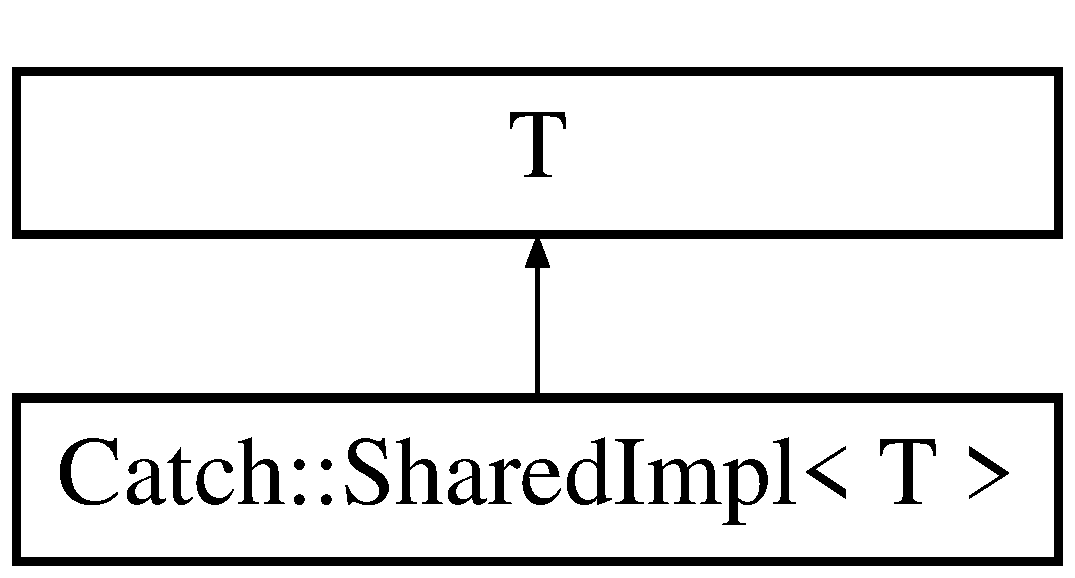
\includegraphics[height=2.000000cm]{struct_catch_1_1_shared_impl}
\end{center}
\end{figure}
\subsection*{Public Member Functions}
\begin{DoxyCompactItemize}
\item 
\mbox{\hyperlink{struct_catch_1_1_shared_impl_a0629856ee353298b61ad52cf60e716fb}{Shared\+Impl}} ()
\item 
virtual void \mbox{\hyperlink{struct_catch_1_1_shared_impl_a5d1a4c96e8fc07c821890fd09749062e}{add\+Ref}} () const
\item 
virtual void \mbox{\hyperlink{struct_catch_1_1_shared_impl_ada8052c6f24fd73ec099333626f106fe}{release}} () const
\end{DoxyCompactItemize}
\subsection*{Public Attributes}
\begin{DoxyCompactItemize}
\item 
unsigned int \mbox{\hyperlink{struct_catch_1_1_shared_impl_a7e71ef1985b85aa41a1632f932a96bcb}{m\+\_\+rc}}
\end{DoxyCompactItemize}


\subsection{Constructor \& Destructor Documentation}
\mbox{\Hypertarget{struct_catch_1_1_shared_impl_a0629856ee353298b61ad52cf60e716fb}\label{struct_catch_1_1_shared_impl_a0629856ee353298b61ad52cf60e716fb}} 
\index{Catch\+::\+Shared\+Impl@{Catch\+::\+Shared\+Impl}!Shared\+Impl@{Shared\+Impl}}
\index{Shared\+Impl@{Shared\+Impl}!Catch\+::\+Shared\+Impl@{Catch\+::\+Shared\+Impl}}
\subsubsection{\texorpdfstring{Shared\+Impl()}{SharedImpl()}}
{\footnotesize\ttfamily template$<$typename T = I\+Shared$>$ \\
\mbox{\hyperlink{struct_catch_1_1_shared_impl}{Catch\+::\+Shared\+Impl}}$<$ T $>$\+::\mbox{\hyperlink{struct_catch_1_1_shared_impl}{Shared\+Impl}} (\begin{DoxyParamCaption}{ }\end{DoxyParamCaption})\hspace{0.3cm}{\ttfamily [inline]}}



\subsection{Member Function Documentation}
\mbox{\Hypertarget{struct_catch_1_1_shared_impl_a5d1a4c96e8fc07c821890fd09749062e}\label{struct_catch_1_1_shared_impl_a5d1a4c96e8fc07c821890fd09749062e}} 
\index{Catch\+::\+Shared\+Impl@{Catch\+::\+Shared\+Impl}!add\+Ref@{add\+Ref}}
\index{add\+Ref@{add\+Ref}!Catch\+::\+Shared\+Impl@{Catch\+::\+Shared\+Impl}}
\subsubsection{\texorpdfstring{add\+Ref()}{addRef()}}
{\footnotesize\ttfamily template$<$typename T = I\+Shared$>$ \\
virtual void \mbox{\hyperlink{struct_catch_1_1_shared_impl}{Catch\+::\+Shared\+Impl}}$<$ T $>$\+::add\+Ref (\begin{DoxyParamCaption}{ }\end{DoxyParamCaption}) const\hspace{0.3cm}{\ttfamily [inline]}, {\ttfamily [virtual]}}

\mbox{\Hypertarget{struct_catch_1_1_shared_impl_ada8052c6f24fd73ec099333626f106fe}\label{struct_catch_1_1_shared_impl_ada8052c6f24fd73ec099333626f106fe}} 
\index{Catch\+::\+Shared\+Impl@{Catch\+::\+Shared\+Impl}!release@{release}}
\index{release@{release}!Catch\+::\+Shared\+Impl@{Catch\+::\+Shared\+Impl}}
\subsubsection{\texorpdfstring{release()}{release()}}
{\footnotesize\ttfamily template$<$typename T = I\+Shared$>$ \\
virtual void \mbox{\hyperlink{struct_catch_1_1_shared_impl}{Catch\+::\+Shared\+Impl}}$<$ T $>$\+::release (\begin{DoxyParamCaption}{ }\end{DoxyParamCaption}) const\hspace{0.3cm}{\ttfamily [inline]}, {\ttfamily [virtual]}}



\subsection{Member Data Documentation}
\mbox{\Hypertarget{struct_catch_1_1_shared_impl_a7e71ef1985b85aa41a1632f932a96bcb}\label{struct_catch_1_1_shared_impl_a7e71ef1985b85aa41a1632f932a96bcb}} 
\index{Catch\+::\+Shared\+Impl@{Catch\+::\+Shared\+Impl}!m\+\_\+rc@{m\+\_\+rc}}
\index{m\+\_\+rc@{m\+\_\+rc}!Catch\+::\+Shared\+Impl@{Catch\+::\+Shared\+Impl}}
\subsubsection{\texorpdfstring{m\+\_\+rc}{m\_rc}}
{\footnotesize\ttfamily template$<$typename T = I\+Shared$>$ \\
unsigned int \mbox{\hyperlink{struct_catch_1_1_shared_impl}{Catch\+::\+Shared\+Impl}}$<$ T $>$\+::m\+\_\+rc\hspace{0.3cm}{\ttfamily [mutable]}}



The documentation for this struct was generated from the following file\+:\begin{DoxyCompactItemize}
\item 
include/\mbox{\hyperlink{catch_8hpp}{catch.\+hpp}}\end{DoxyCompactItemize}

\hypertarget{struct_catch_1_1_source_line_info}{}\section{Catch\+:\+:Source\+Line\+Info Struct Reference}
\label{struct_catch_1_1_source_line_info}\index{Catch\+::\+Source\+Line\+Info@{Catch\+::\+Source\+Line\+Info}}


{\ttfamily \#include $<$catch.\+hpp$>$}

\subsection*{Public Member Functions}
\begin{DoxyCompactItemize}
\item 
\mbox{\hyperlink{struct_catch_1_1_source_line_info_a9d44b2e1133794eee0bd5716424c83d6}{Source\+Line\+Info}} ()
\item 
\mbox{\hyperlink{struct_catch_1_1_source_line_info_a6218cb890337d37f708ea94063958940}{Source\+Line\+Info}} (char const $\ast$\+\_\+file, std\+::size\+\_\+t \+\_\+line)
\item 
bool \mbox{\hyperlink{struct_catch_1_1_source_line_info_a05ab6444e9de7e9c3e76d8aa00093c3a}{empty}} () const
\item 
bool \mbox{\hyperlink{struct_catch_1_1_source_line_info_a688e761986879266658f000f14ab8a42}{operator==}} (\mbox{\hyperlink{struct_catch_1_1_source_line_info}{Source\+Line\+Info}} const \&other) const
\item 
bool \mbox{\hyperlink{struct_catch_1_1_source_line_info_a8b99a0d7b1553d8c2298c694db924be3}{operator$<$}} (\mbox{\hyperlink{struct_catch_1_1_source_line_info}{Source\+Line\+Info}} const \&other) const
\end{DoxyCompactItemize}
\subsection*{Public Attributes}
\begin{DoxyCompactItemize}
\item 
char const  $\ast$ \mbox{\hyperlink{struct_catch_1_1_source_line_info_ad65537703e9f08c1fa7777fbc3f0c617}{file}}
\item 
std\+::size\+\_\+t \mbox{\hyperlink{struct_catch_1_1_source_line_info_a841e5d696c7b9cde24e45e61dd979c77}{line}}
\end{DoxyCompactItemize}


\subsection{Constructor \& Destructor Documentation}
\mbox{\Hypertarget{struct_catch_1_1_source_line_info_a9d44b2e1133794eee0bd5716424c83d6}\label{struct_catch_1_1_source_line_info_a9d44b2e1133794eee0bd5716424c83d6}} 
\index{Catch\+::\+Source\+Line\+Info@{Catch\+::\+Source\+Line\+Info}!Source\+Line\+Info@{Source\+Line\+Info}}
\index{Source\+Line\+Info@{Source\+Line\+Info}!Catch\+::\+Source\+Line\+Info@{Catch\+::\+Source\+Line\+Info}}
\subsubsection{\texorpdfstring{Source\+Line\+Info()}{SourceLineInfo()}\hspace{0.1cm}{\footnotesize\ttfamily [1/2]}}
{\footnotesize\ttfamily Catch\+::\+Source\+Line\+Info\+::\+Source\+Line\+Info (\begin{DoxyParamCaption}{ }\end{DoxyParamCaption})}

\mbox{\Hypertarget{struct_catch_1_1_source_line_info_a6218cb890337d37f708ea94063958940}\label{struct_catch_1_1_source_line_info_a6218cb890337d37f708ea94063958940}} 
\index{Catch\+::\+Source\+Line\+Info@{Catch\+::\+Source\+Line\+Info}!Source\+Line\+Info@{Source\+Line\+Info}}
\index{Source\+Line\+Info@{Source\+Line\+Info}!Catch\+::\+Source\+Line\+Info@{Catch\+::\+Source\+Line\+Info}}
\subsubsection{\texorpdfstring{Source\+Line\+Info()}{SourceLineInfo()}\hspace{0.1cm}{\footnotesize\ttfamily [2/2]}}
{\footnotesize\ttfamily Catch\+::\+Source\+Line\+Info\+::\+Source\+Line\+Info (\begin{DoxyParamCaption}\item[{char const $\ast$}]{\+\_\+file,  }\item[{std\+::size\+\_\+t}]{\+\_\+line }\end{DoxyParamCaption})}



\subsection{Member Function Documentation}
\mbox{\Hypertarget{struct_catch_1_1_source_line_info_a05ab6444e9de7e9c3e76d8aa00093c3a}\label{struct_catch_1_1_source_line_info_a05ab6444e9de7e9c3e76d8aa00093c3a}} 
\index{Catch\+::\+Source\+Line\+Info@{Catch\+::\+Source\+Line\+Info}!empty@{empty}}
\index{empty@{empty}!Catch\+::\+Source\+Line\+Info@{Catch\+::\+Source\+Line\+Info}}
\subsubsection{\texorpdfstring{empty()}{empty()}}
{\footnotesize\ttfamily bool Catch\+::\+Source\+Line\+Info\+::empty (\begin{DoxyParamCaption}{ }\end{DoxyParamCaption}) const}

\mbox{\Hypertarget{struct_catch_1_1_source_line_info_a8b99a0d7b1553d8c2298c694db924be3}\label{struct_catch_1_1_source_line_info_a8b99a0d7b1553d8c2298c694db924be3}} 
\index{Catch\+::\+Source\+Line\+Info@{Catch\+::\+Source\+Line\+Info}!operator$<$@{operator$<$}}
\index{operator$<$@{operator$<$}!Catch\+::\+Source\+Line\+Info@{Catch\+::\+Source\+Line\+Info}}
\subsubsection{\texorpdfstring{operator$<$()}{operator<()}}
{\footnotesize\ttfamily bool Catch\+::\+Source\+Line\+Info\+::operator$<$ (\begin{DoxyParamCaption}\item[{\mbox{\hyperlink{struct_catch_1_1_source_line_info}{Source\+Line\+Info}} const \&}]{other }\end{DoxyParamCaption}) const}

\mbox{\Hypertarget{struct_catch_1_1_source_line_info_a688e761986879266658f000f14ab8a42}\label{struct_catch_1_1_source_line_info_a688e761986879266658f000f14ab8a42}} 
\index{Catch\+::\+Source\+Line\+Info@{Catch\+::\+Source\+Line\+Info}!operator==@{operator==}}
\index{operator==@{operator==}!Catch\+::\+Source\+Line\+Info@{Catch\+::\+Source\+Line\+Info}}
\subsubsection{\texorpdfstring{operator==()}{operator==()}}
{\footnotesize\ttfamily bool Catch\+::\+Source\+Line\+Info\+::operator== (\begin{DoxyParamCaption}\item[{\mbox{\hyperlink{struct_catch_1_1_source_line_info}{Source\+Line\+Info}} const \&}]{other }\end{DoxyParamCaption}) const}



\subsection{Member Data Documentation}
\mbox{\Hypertarget{struct_catch_1_1_source_line_info_ad65537703e9f08c1fa7777fbc3f0c617}\label{struct_catch_1_1_source_line_info_ad65537703e9f08c1fa7777fbc3f0c617}} 
\index{Catch\+::\+Source\+Line\+Info@{Catch\+::\+Source\+Line\+Info}!file@{file}}
\index{file@{file}!Catch\+::\+Source\+Line\+Info@{Catch\+::\+Source\+Line\+Info}}
\subsubsection{\texorpdfstring{file}{file}}
{\footnotesize\ttfamily char const$\ast$ Catch\+::\+Source\+Line\+Info\+::file}

\mbox{\Hypertarget{struct_catch_1_1_source_line_info_a841e5d696c7b9cde24e45e61dd979c77}\label{struct_catch_1_1_source_line_info_a841e5d696c7b9cde24e45e61dd979c77}} 
\index{Catch\+::\+Source\+Line\+Info@{Catch\+::\+Source\+Line\+Info}!line@{line}}
\index{line@{line}!Catch\+::\+Source\+Line\+Info@{Catch\+::\+Source\+Line\+Info}}
\subsubsection{\texorpdfstring{line}{line}}
{\footnotesize\ttfamily std\+::size\+\_\+t Catch\+::\+Source\+Line\+Info\+::line}



The documentation for this struct was generated from the following file\+:\begin{DoxyCompactItemize}
\item 
include/\mbox{\hyperlink{catch_8hpp}{catch.\+hpp}}\end{DoxyCompactItemize}

\hypertarget{struct_catch_1_1_matchers_1_1_std_string_1_1_starts_with_matcher}{}\section{Catch\+:\+:Matchers\+:\+:Std\+String\+:\+:Starts\+With\+Matcher Struct Reference}
\label{struct_catch_1_1_matchers_1_1_std_string_1_1_starts_with_matcher}\index{Catch\+::\+Matchers\+::\+Std\+String\+::\+Starts\+With\+Matcher@{Catch\+::\+Matchers\+::\+Std\+String\+::\+Starts\+With\+Matcher}}


{\ttfamily \#include $<$catch.\+hpp$>$}

Inheritance diagram for Catch\+:\+:Matchers\+:\+:Std\+String\+:\+:Starts\+With\+Matcher\+:\begin{figure}[H]
\begin{center}
\leavevmode
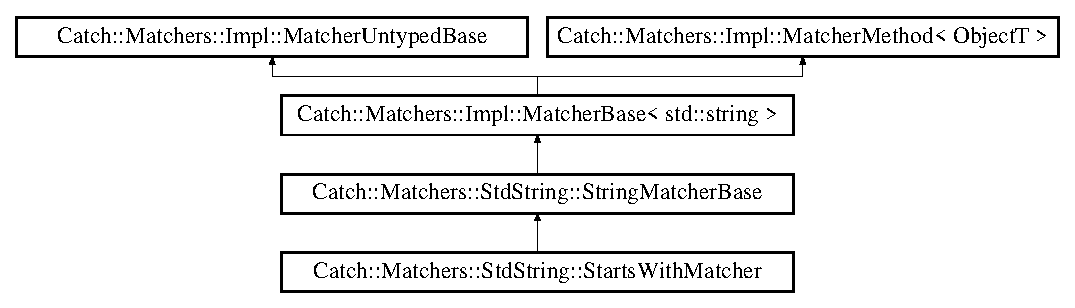
\includegraphics[height=3.696370cm]{struct_catch_1_1_matchers_1_1_std_string_1_1_starts_with_matcher}
\end{center}
\end{figure}
\subsection*{Public Member Functions}
\begin{DoxyCompactItemize}
\item 
\mbox{\hyperlink{struct_catch_1_1_matchers_1_1_std_string_1_1_starts_with_matcher_a7b86f258bdbd131a6e7bcd94a8977325}{Starts\+With\+Matcher}} (\mbox{\hyperlink{struct_catch_1_1_matchers_1_1_std_string_1_1_cased_string}{Cased\+String}} const \&comparator)
\item 
virtual bool \mbox{\hyperlink{struct_catch_1_1_matchers_1_1_std_string_1_1_starts_with_matcher_a0d37b1ddba7f1031e360ccd475f05d0d}{match}} (std\+::string const \&source) const \mbox{\hyperlink{catch_8hpp_a8ecdce4d3f57835f707915ae831eb847}{C\+A\+T\+C\+H\+\_\+\+O\+V\+E\+R\+R\+I\+DE}}
\end{DoxyCompactItemize}
\subsection*{Additional Inherited Members}


\subsection{Constructor \& Destructor Documentation}
\mbox{\Hypertarget{struct_catch_1_1_matchers_1_1_std_string_1_1_starts_with_matcher_a7b86f258bdbd131a6e7bcd94a8977325}\label{struct_catch_1_1_matchers_1_1_std_string_1_1_starts_with_matcher_a7b86f258bdbd131a6e7bcd94a8977325}} 
\index{Catch\+::\+Matchers\+::\+Std\+String\+::\+Starts\+With\+Matcher@{Catch\+::\+Matchers\+::\+Std\+String\+::\+Starts\+With\+Matcher}!Starts\+With\+Matcher@{Starts\+With\+Matcher}}
\index{Starts\+With\+Matcher@{Starts\+With\+Matcher}!Catch\+::\+Matchers\+::\+Std\+String\+::\+Starts\+With\+Matcher@{Catch\+::\+Matchers\+::\+Std\+String\+::\+Starts\+With\+Matcher}}
\subsubsection{\texorpdfstring{Starts\+With\+Matcher()}{StartsWithMatcher()}}
{\footnotesize\ttfamily Catch\+::\+Matchers\+::\+Std\+String\+::\+Starts\+With\+Matcher\+::\+Starts\+With\+Matcher (\begin{DoxyParamCaption}\item[{\mbox{\hyperlink{struct_catch_1_1_matchers_1_1_std_string_1_1_cased_string}{Cased\+String}} const \&}]{comparator }\end{DoxyParamCaption})}



\subsection{Member Function Documentation}
\mbox{\Hypertarget{struct_catch_1_1_matchers_1_1_std_string_1_1_starts_with_matcher_a0d37b1ddba7f1031e360ccd475f05d0d}\label{struct_catch_1_1_matchers_1_1_std_string_1_1_starts_with_matcher_a0d37b1ddba7f1031e360ccd475f05d0d}} 
\index{Catch\+::\+Matchers\+::\+Std\+String\+::\+Starts\+With\+Matcher@{Catch\+::\+Matchers\+::\+Std\+String\+::\+Starts\+With\+Matcher}!match@{match}}
\index{match@{match}!Catch\+::\+Matchers\+::\+Std\+String\+::\+Starts\+With\+Matcher@{Catch\+::\+Matchers\+::\+Std\+String\+::\+Starts\+With\+Matcher}}
\subsubsection{\texorpdfstring{match()}{match()}}
{\footnotesize\ttfamily virtual bool Catch\+::\+Matchers\+::\+Std\+String\+::\+Starts\+With\+Matcher\+::match (\begin{DoxyParamCaption}\item[{std\+::string const \&}]{source }\end{DoxyParamCaption}) const\hspace{0.3cm}{\ttfamily [virtual]}}



The documentation for this struct was generated from the following file\+:\begin{DoxyCompactItemize}
\item 
include/\mbox{\hyperlink{catch_8hpp}{catch.\+hpp}}\end{DoxyCompactItemize}

\hypertarget{struct_catch_1_1_stream_end_stop}{}\section{Catch\+:\+:Stream\+End\+Stop Struct Reference}
\label{struct_catch_1_1_stream_end_stop}\index{Catch\+::\+Stream\+End\+Stop@{Catch\+::\+Stream\+End\+Stop}}


{\ttfamily \#include $<$catch.\+hpp$>$}

\subsection*{Public Member Functions}
\begin{DoxyCompactItemize}
\item 
std\+::string \mbox{\hyperlink{struct_catch_1_1_stream_end_stop_a3025092e06c224e0845f2caa07b26d0e}{operator+}} ()
\end{DoxyCompactItemize}


\subsection{Member Function Documentation}
\mbox{\Hypertarget{struct_catch_1_1_stream_end_stop_a3025092e06c224e0845f2caa07b26d0e}\label{struct_catch_1_1_stream_end_stop_a3025092e06c224e0845f2caa07b26d0e}} 
\index{Catch\+::\+Stream\+End\+Stop@{Catch\+::\+Stream\+End\+Stop}!operator+@{operator+}}
\index{operator+@{operator+}!Catch\+::\+Stream\+End\+Stop@{Catch\+::\+Stream\+End\+Stop}}
\subsubsection{\texorpdfstring{operator+()}{operator+()}}
{\footnotesize\ttfamily std\+::string Catch\+::\+Stream\+End\+Stop\+::operator+ (\begin{DoxyParamCaption}{ }\end{DoxyParamCaption})\hspace{0.3cm}{\ttfamily [inline]}}



The documentation for this struct was generated from the following file\+:\begin{DoxyCompactItemize}
\item 
include/\mbox{\hyperlink{catch_8hpp}{catch.\+hpp}}\end{DoxyCompactItemize}

\hypertarget{struct_catch_1_1_string_maker}{}\section{Catch\+:\+:String\+Maker$<$ T $>$ Struct Template Reference}
\label{struct_catch_1_1_string_maker}\index{Catch\+::\+String\+Maker$<$ T $>$@{Catch\+::\+String\+Maker$<$ T $>$}}


{\ttfamily \#include $<$catch.\+hpp$>$}

Inheritance diagram for Catch\+:\+:String\+Maker$<$ T $>$\+:\begin{figure}[H]
\begin{center}
\leavevmode
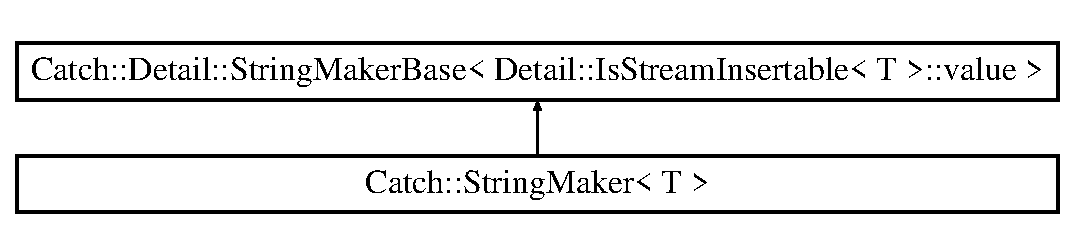
\includegraphics[height=2.000000cm]{struct_catch_1_1_string_maker}
\end{center}
\end{figure}
\subsection*{Additional Inherited Members}


The documentation for this struct was generated from the following file\+:\begin{DoxyCompactItemize}
\item 
include/\mbox{\hyperlink{catch_8hpp}{catch.\+hpp}}\end{DoxyCompactItemize}

\hypertarget{struct_catch_1_1_string_maker_3_01_r_01_c_1_1_5_01_4}{}\section{Catch\+:\+:String\+Maker$<$ R C\+:\+:$\ast$ $>$ Struct Template Reference}
\label{struct_catch_1_1_string_maker_3_01_r_01_c_1_1_5_01_4}\index{Catch\+::\+String\+Maker$<$ R C\+::$\ast$ $>$@{Catch\+::\+String\+Maker$<$ R C\+::$\ast$ $>$}}


{\ttfamily \#include $<$catch.\+hpp$>$}

\subsection*{Static Public Member Functions}
\begin{DoxyCompactItemize}
\item 
static std\+::string \mbox{\hyperlink{struct_catch_1_1_string_maker_3_01_r_01_c_1_1_5_01_4_af69c15e0b406e945777137fe4a333731}{convert}} (R C\+::$\ast$p)
\end{DoxyCompactItemize}


\subsection{Member Function Documentation}
\mbox{\Hypertarget{struct_catch_1_1_string_maker_3_01_r_01_c_1_1_5_01_4_af69c15e0b406e945777137fe4a333731}\label{struct_catch_1_1_string_maker_3_01_r_01_c_1_1_5_01_4_af69c15e0b406e945777137fe4a333731}} 
\index{Catch\+::\+String\+Maker$<$ R C\+::$\ast$ $>$@{Catch\+::\+String\+Maker$<$ R C\+::$\ast$ $>$}!convert@{convert}}
\index{convert@{convert}!Catch\+::\+String\+Maker$<$ R C\+::$\ast$ $>$@{Catch\+::\+String\+Maker$<$ R C\+::$\ast$ $>$}}
\subsubsection{\texorpdfstring{convert()}{convert()}}
{\footnotesize\ttfamily template$<$typename R , typename C $>$ \\
static std\+::string \mbox{\hyperlink{struct_catch_1_1_string_maker}{Catch\+::\+String\+Maker}}$<$ R C\+::$\ast$ $>$\+::convert (\begin{DoxyParamCaption}\item[{R C\+::$\ast$}]{p }\end{DoxyParamCaption})\hspace{0.3cm}{\ttfamily [inline]}, {\ttfamily [static]}}



The documentation for this struct was generated from the following file\+:\begin{DoxyCompactItemize}
\item 
include/\mbox{\hyperlink{catch_8hpp}{catch.\+hpp}}\end{DoxyCompactItemize}

\hypertarget{struct_catch_1_1_string_maker_3_01_t_01_5_01_4}{}\section{Catch\+:\+:String\+Maker$<$ T $\ast$ $>$ Struct Template Reference}
\label{struct_catch_1_1_string_maker_3_01_t_01_5_01_4}\index{Catch\+::\+String\+Maker$<$ T $\ast$ $>$@{Catch\+::\+String\+Maker$<$ T $\ast$ $>$}}


{\ttfamily \#include $<$catch.\+hpp$>$}

\subsection*{Static Public Member Functions}
\begin{DoxyCompactItemize}
\item 
{\footnotesize template$<$typename U $>$ }\\static std\+::string \mbox{\hyperlink{struct_catch_1_1_string_maker_3_01_t_01_5_01_4_a2adbc75c99d71b8323f4052bcb0815c9}{convert}} (U $\ast$p)
\end{DoxyCompactItemize}


\subsection{Member Function Documentation}
\mbox{\Hypertarget{struct_catch_1_1_string_maker_3_01_t_01_5_01_4_a2adbc75c99d71b8323f4052bcb0815c9}\label{struct_catch_1_1_string_maker_3_01_t_01_5_01_4_a2adbc75c99d71b8323f4052bcb0815c9}} 
\index{Catch\+::\+String\+Maker$<$ T $\ast$ $>$@{Catch\+::\+String\+Maker$<$ T $\ast$ $>$}!convert@{convert}}
\index{convert@{convert}!Catch\+::\+String\+Maker$<$ T $\ast$ $>$@{Catch\+::\+String\+Maker$<$ T $\ast$ $>$}}
\subsubsection{\texorpdfstring{convert()}{convert()}}
{\footnotesize\ttfamily template$<$typename T $>$ \\
template$<$typename U $>$ \\
static std\+::string \mbox{\hyperlink{struct_catch_1_1_string_maker}{Catch\+::\+String\+Maker}}$<$ T $\ast$ $>$\+::convert (\begin{DoxyParamCaption}\item[{U $\ast$}]{p }\end{DoxyParamCaption})\hspace{0.3cm}{\ttfamily [inline]}, {\ttfamily [static]}}



The documentation for this struct was generated from the following file\+:\begin{DoxyCompactItemize}
\item 
include/\mbox{\hyperlink{catch_8hpp}{catch.\+hpp}}\end{DoxyCompactItemize}

\hypertarget{struct_catch_1_1_detail_1_1_string_maker_base}{}\section{Catch\+:\+:Detail\+:\+:String\+Maker\+Base$<$ C $>$ Struct Template Reference}
\label{struct_catch_1_1_detail_1_1_string_maker_base}\index{Catch\+::\+Detail\+::\+String\+Maker\+Base$<$ C $>$@{Catch\+::\+Detail\+::\+String\+Maker\+Base$<$ C $>$}}


{\ttfamily \#include $<$catch.\+hpp$>$}

\subsection*{Static Public Member Functions}
\begin{DoxyCompactItemize}
\item 
{\footnotesize template$<$typename T $>$ }\\static std\+::string \mbox{\hyperlink{struct_catch_1_1_detail_1_1_string_maker_base_a8eb9f635dc413a5758e22614bafaf1a3}{convert}} (T const \&)
\end{DoxyCompactItemize}


\subsection{Member Function Documentation}
\mbox{\Hypertarget{struct_catch_1_1_detail_1_1_string_maker_base_a8eb9f635dc413a5758e22614bafaf1a3}\label{struct_catch_1_1_detail_1_1_string_maker_base_a8eb9f635dc413a5758e22614bafaf1a3}} 
\index{Catch\+::\+Detail\+::\+String\+Maker\+Base@{Catch\+::\+Detail\+::\+String\+Maker\+Base}!convert@{convert}}
\index{convert@{convert}!Catch\+::\+Detail\+::\+String\+Maker\+Base@{Catch\+::\+Detail\+::\+String\+Maker\+Base}}
\subsubsection{\texorpdfstring{convert()}{convert()}}
{\footnotesize\ttfamily template$<$bool C$>$ \\
template$<$typename T $>$ \\
static std\+::string \mbox{\hyperlink{struct_catch_1_1_detail_1_1_string_maker_base}{Catch\+::\+Detail\+::\+String\+Maker\+Base}}$<$ C $>$\+::convert (\begin{DoxyParamCaption}\item[{T const \&}]{ }\end{DoxyParamCaption})\hspace{0.3cm}{\ttfamily [inline]}, {\ttfamily [static]}}



The documentation for this struct was generated from the following file\+:\begin{DoxyCompactItemize}
\item 
include/\mbox{\hyperlink{catch_8hpp}{catch.\+hpp}}\end{DoxyCompactItemize}

\hypertarget{struct_catch_1_1_detail_1_1_string_maker_base_3_01true_01_4}{}\section{Catch\+:\+:Detail\+:\+:String\+Maker\+Base$<$ true $>$ Struct Template Reference}
\label{struct_catch_1_1_detail_1_1_string_maker_base_3_01true_01_4}\index{Catch\+::\+Detail\+::\+String\+Maker\+Base$<$ true $>$@{Catch\+::\+Detail\+::\+String\+Maker\+Base$<$ true $>$}}


{\ttfamily \#include $<$catch.\+hpp$>$}

\subsection*{Static Public Member Functions}
\begin{DoxyCompactItemize}
\item 
{\footnotesize template$<$typename T $>$ }\\static std\+::string \mbox{\hyperlink{struct_catch_1_1_detail_1_1_string_maker_base_3_01true_01_4_af9b5fdf7fddd8c5c873caa819e5f00f6}{convert}} (T const \&\+\_\+value)
\end{DoxyCompactItemize}


\subsection{Member Function Documentation}
\mbox{\Hypertarget{struct_catch_1_1_detail_1_1_string_maker_base_3_01true_01_4_af9b5fdf7fddd8c5c873caa819e5f00f6}\label{struct_catch_1_1_detail_1_1_string_maker_base_3_01true_01_4_af9b5fdf7fddd8c5c873caa819e5f00f6}} 
\index{Catch\+::\+Detail\+::\+String\+Maker\+Base$<$ true $>$@{Catch\+::\+Detail\+::\+String\+Maker\+Base$<$ true $>$}!convert@{convert}}
\index{convert@{convert}!Catch\+::\+Detail\+::\+String\+Maker\+Base$<$ true $>$@{Catch\+::\+Detail\+::\+String\+Maker\+Base$<$ true $>$}}
\subsubsection{\texorpdfstring{convert()}{convert()}}
{\footnotesize\ttfamily template$<$typename T $>$ \\
static std\+::string \mbox{\hyperlink{struct_catch_1_1_detail_1_1_string_maker_base}{Catch\+::\+Detail\+::\+String\+Maker\+Base}}$<$ true $>$\+::convert (\begin{DoxyParamCaption}\item[{T const \&}]{\+\_\+value }\end{DoxyParamCaption})\hspace{0.3cm}{\ttfamily [inline]}, {\ttfamily [static]}}



The documentation for this struct was generated from the following file\+:\begin{DoxyCompactItemize}
\item 
include/\mbox{\hyperlink{catch_8hpp}{catch.\+hpp}}\end{DoxyCompactItemize}

\hypertarget{struct_catch_1_1_matchers_1_1_std_string_1_1_string_matcher_base}{}\section{Catch\+:\+:Matchers\+:\+:Std\+String\+:\+:String\+Matcher\+Base Struct Reference}
\label{struct_catch_1_1_matchers_1_1_std_string_1_1_string_matcher_base}\index{Catch\+::\+Matchers\+::\+Std\+String\+::\+String\+Matcher\+Base@{Catch\+::\+Matchers\+::\+Std\+String\+::\+String\+Matcher\+Base}}


{\ttfamily \#include $<$catch.\+hpp$>$}

Inheritance diagram for Catch\+:\+:Matchers\+:\+:Std\+String\+:\+:String\+Matcher\+Base\+:\begin{figure}[H]
\begin{center}
\leavevmode
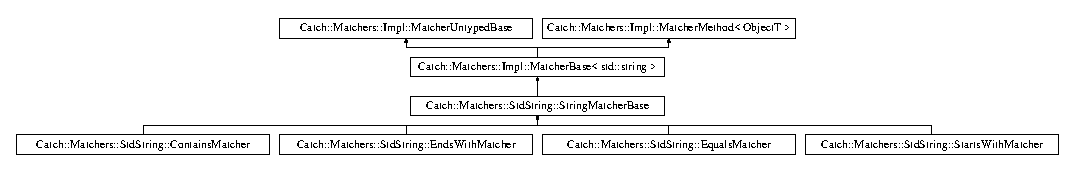
\includegraphics[height=1.848185cm]{struct_catch_1_1_matchers_1_1_std_string_1_1_string_matcher_base}
\end{center}
\end{figure}
\subsection*{Public Member Functions}
\begin{DoxyCompactItemize}
\item 
\mbox{\hyperlink{struct_catch_1_1_matchers_1_1_std_string_1_1_string_matcher_base_a3a9b66bae298ae27058478529b4bb39d}{String\+Matcher\+Base}} (std\+::string const \&operation, \mbox{\hyperlink{struct_catch_1_1_matchers_1_1_std_string_1_1_cased_string}{Cased\+String}} const \&comparator)
\item 
virtual std\+::string \mbox{\hyperlink{struct_catch_1_1_matchers_1_1_std_string_1_1_string_matcher_base_a9d15cfb882efbea778b2ed29e7f48f37}{describe}} () const \mbox{\hyperlink{catch_8hpp_a8ecdce4d3f57835f707915ae831eb847}{C\+A\+T\+C\+H\+\_\+\+O\+V\+E\+R\+R\+I\+DE}}
\end{DoxyCompactItemize}
\subsection*{Public Attributes}
\begin{DoxyCompactItemize}
\item 
\mbox{\hyperlink{struct_catch_1_1_matchers_1_1_std_string_1_1_cased_string}{Cased\+String}} \mbox{\hyperlink{struct_catch_1_1_matchers_1_1_std_string_1_1_string_matcher_base_a17c9f0fe40587070ffe998c193742831}{m\+\_\+comparator}}
\item 
std\+::string \mbox{\hyperlink{struct_catch_1_1_matchers_1_1_std_string_1_1_string_matcher_base_a7a25c4b7d863e9a1c406d81efd0f83ca}{m\+\_\+operation}}
\end{DoxyCompactItemize}
\subsection*{Additional Inherited Members}


\subsection{Constructor \& Destructor Documentation}
\mbox{\Hypertarget{struct_catch_1_1_matchers_1_1_std_string_1_1_string_matcher_base_a3a9b66bae298ae27058478529b4bb39d}\label{struct_catch_1_1_matchers_1_1_std_string_1_1_string_matcher_base_a3a9b66bae298ae27058478529b4bb39d}} 
\index{Catch\+::\+Matchers\+::\+Std\+String\+::\+String\+Matcher\+Base@{Catch\+::\+Matchers\+::\+Std\+String\+::\+String\+Matcher\+Base}!String\+Matcher\+Base@{String\+Matcher\+Base}}
\index{String\+Matcher\+Base@{String\+Matcher\+Base}!Catch\+::\+Matchers\+::\+Std\+String\+::\+String\+Matcher\+Base@{Catch\+::\+Matchers\+::\+Std\+String\+::\+String\+Matcher\+Base}}
\subsubsection{\texorpdfstring{String\+Matcher\+Base()}{StringMatcherBase()}}
{\footnotesize\ttfamily Catch\+::\+Matchers\+::\+Std\+String\+::\+String\+Matcher\+Base\+::\+String\+Matcher\+Base (\begin{DoxyParamCaption}\item[{std\+::string const \&}]{operation,  }\item[{\mbox{\hyperlink{struct_catch_1_1_matchers_1_1_std_string_1_1_cased_string}{Cased\+String}} const \&}]{comparator }\end{DoxyParamCaption})}



\subsection{Member Function Documentation}
\mbox{\Hypertarget{struct_catch_1_1_matchers_1_1_std_string_1_1_string_matcher_base_a9d15cfb882efbea778b2ed29e7f48f37}\label{struct_catch_1_1_matchers_1_1_std_string_1_1_string_matcher_base_a9d15cfb882efbea778b2ed29e7f48f37}} 
\index{Catch\+::\+Matchers\+::\+Std\+String\+::\+String\+Matcher\+Base@{Catch\+::\+Matchers\+::\+Std\+String\+::\+String\+Matcher\+Base}!describe@{describe}}
\index{describe@{describe}!Catch\+::\+Matchers\+::\+Std\+String\+::\+String\+Matcher\+Base@{Catch\+::\+Matchers\+::\+Std\+String\+::\+String\+Matcher\+Base}}
\subsubsection{\texorpdfstring{describe()}{describe()}}
{\footnotesize\ttfamily virtual std\+::string Catch\+::\+Matchers\+::\+Std\+String\+::\+String\+Matcher\+Base\+::describe (\begin{DoxyParamCaption}{ }\end{DoxyParamCaption}) const\hspace{0.3cm}{\ttfamily [virtual]}}



Implements \mbox{\hyperlink{class_catch_1_1_matchers_1_1_impl_1_1_matcher_untyped_base_a91d3a907dbfcbb596077df24f6e11fe2}{Catch\+::\+Matchers\+::\+Impl\+::\+Matcher\+Untyped\+Base}}.



\subsection{Member Data Documentation}
\mbox{\Hypertarget{struct_catch_1_1_matchers_1_1_std_string_1_1_string_matcher_base_a17c9f0fe40587070ffe998c193742831}\label{struct_catch_1_1_matchers_1_1_std_string_1_1_string_matcher_base_a17c9f0fe40587070ffe998c193742831}} 
\index{Catch\+::\+Matchers\+::\+Std\+String\+::\+String\+Matcher\+Base@{Catch\+::\+Matchers\+::\+Std\+String\+::\+String\+Matcher\+Base}!m\+\_\+comparator@{m\+\_\+comparator}}
\index{m\+\_\+comparator@{m\+\_\+comparator}!Catch\+::\+Matchers\+::\+Std\+String\+::\+String\+Matcher\+Base@{Catch\+::\+Matchers\+::\+Std\+String\+::\+String\+Matcher\+Base}}
\subsubsection{\texorpdfstring{m\+\_\+comparator}{m\_comparator}}
{\footnotesize\ttfamily \mbox{\hyperlink{struct_catch_1_1_matchers_1_1_std_string_1_1_cased_string}{Cased\+String}} Catch\+::\+Matchers\+::\+Std\+String\+::\+String\+Matcher\+Base\+::m\+\_\+comparator}

\mbox{\Hypertarget{struct_catch_1_1_matchers_1_1_std_string_1_1_string_matcher_base_a7a25c4b7d863e9a1c406d81efd0f83ca}\label{struct_catch_1_1_matchers_1_1_std_string_1_1_string_matcher_base_a7a25c4b7d863e9a1c406d81efd0f83ca}} 
\index{Catch\+::\+Matchers\+::\+Std\+String\+::\+String\+Matcher\+Base@{Catch\+::\+Matchers\+::\+Std\+String\+::\+String\+Matcher\+Base}!m\+\_\+operation@{m\+\_\+operation}}
\index{m\+\_\+operation@{m\+\_\+operation}!Catch\+::\+Matchers\+::\+Std\+String\+::\+String\+Matcher\+Base@{Catch\+::\+Matchers\+::\+Std\+String\+::\+String\+Matcher\+Base}}
\subsubsection{\texorpdfstring{m\+\_\+operation}{m\_operation}}
{\footnotesize\ttfamily std\+::string Catch\+::\+Matchers\+::\+Std\+String\+::\+String\+Matcher\+Base\+::m\+\_\+operation}



The documentation for this struct was generated from the following file\+:\begin{DoxyCompactItemize}
\item 
include/\mbox{\hyperlink{catch_8hpp}{catch.\+hpp}}\end{DoxyCompactItemize}

\hypertarget{struct_catch_1_1_tag_alias}{}\section{Catch\+:\+:Tag\+Alias Struct Reference}
\label{struct_catch_1_1_tag_alias}\index{Catch\+::\+Tag\+Alias@{Catch\+::\+Tag\+Alias}}


{\ttfamily \#include $<$catch.\+hpp$>$}

\subsection*{Public Member Functions}
\begin{DoxyCompactItemize}
\item 
\mbox{\hyperlink{struct_catch_1_1_tag_alias_ae5a030edfbc8e37f28310d4ca599396c}{Tag\+Alias}} (std\+::string const \&\+\_\+tag, \mbox{\hyperlink{struct_catch_1_1_source_line_info}{Source\+Line\+Info}} \+\_\+line\+Info)
\end{DoxyCompactItemize}
\subsection*{Public Attributes}
\begin{DoxyCompactItemize}
\item 
std\+::string \mbox{\hyperlink{struct_catch_1_1_tag_alias_a950183883ab17c90d0fab16b966b6e2d}{tag}}
\item 
\mbox{\hyperlink{struct_catch_1_1_source_line_info}{Source\+Line\+Info}} \mbox{\hyperlink{struct_catch_1_1_tag_alias_a2f51fe0b3c052561275d26b6eb88f702}{line\+Info}}
\end{DoxyCompactItemize}


\subsection{Constructor \& Destructor Documentation}
\mbox{\Hypertarget{struct_catch_1_1_tag_alias_ae5a030edfbc8e37f28310d4ca599396c}\label{struct_catch_1_1_tag_alias_ae5a030edfbc8e37f28310d4ca599396c}} 
\index{Catch\+::\+Tag\+Alias@{Catch\+::\+Tag\+Alias}!Tag\+Alias@{Tag\+Alias}}
\index{Tag\+Alias@{Tag\+Alias}!Catch\+::\+Tag\+Alias@{Catch\+::\+Tag\+Alias}}
\subsubsection{\texorpdfstring{Tag\+Alias()}{TagAlias()}}
{\footnotesize\ttfamily Catch\+::\+Tag\+Alias\+::\+Tag\+Alias (\begin{DoxyParamCaption}\item[{std\+::string const \&}]{\+\_\+tag,  }\item[{\mbox{\hyperlink{struct_catch_1_1_source_line_info}{Source\+Line\+Info}}}]{\+\_\+line\+Info }\end{DoxyParamCaption})\hspace{0.3cm}{\ttfamily [inline]}}



\subsection{Member Data Documentation}
\mbox{\Hypertarget{struct_catch_1_1_tag_alias_a2f51fe0b3c052561275d26b6eb88f702}\label{struct_catch_1_1_tag_alias_a2f51fe0b3c052561275d26b6eb88f702}} 
\index{Catch\+::\+Tag\+Alias@{Catch\+::\+Tag\+Alias}!line\+Info@{line\+Info}}
\index{line\+Info@{line\+Info}!Catch\+::\+Tag\+Alias@{Catch\+::\+Tag\+Alias}}
\subsubsection{\texorpdfstring{line\+Info}{lineInfo}}
{\footnotesize\ttfamily \mbox{\hyperlink{struct_catch_1_1_source_line_info}{Source\+Line\+Info}} Catch\+::\+Tag\+Alias\+::line\+Info}

\mbox{\Hypertarget{struct_catch_1_1_tag_alias_a950183883ab17c90d0fab16b966b6e2d}\label{struct_catch_1_1_tag_alias_a950183883ab17c90d0fab16b966b6e2d}} 
\index{Catch\+::\+Tag\+Alias@{Catch\+::\+Tag\+Alias}!tag@{tag}}
\index{tag@{tag}!Catch\+::\+Tag\+Alias@{Catch\+::\+Tag\+Alias}}
\subsubsection{\texorpdfstring{tag}{tag}}
{\footnotesize\ttfamily std\+::string Catch\+::\+Tag\+Alias\+::tag}



The documentation for this struct was generated from the following file\+:\begin{DoxyCompactItemize}
\item 
include/\mbox{\hyperlink{catch_8hpp}{catch.\+hpp}}\end{DoxyCompactItemize}

\hypertarget{class_catch_1_1_test_case}{}\section{Catch\+:\+:Test\+Case Class Reference}
\label{class_catch_1_1_test_case}\index{Catch\+::\+Test\+Case@{Catch\+::\+Test\+Case}}


{\ttfamily \#include $<$catch.\+hpp$>$}

Inheritance diagram for Catch\+:\+:Test\+Case\+:\begin{figure}[H]
\begin{center}
\leavevmode
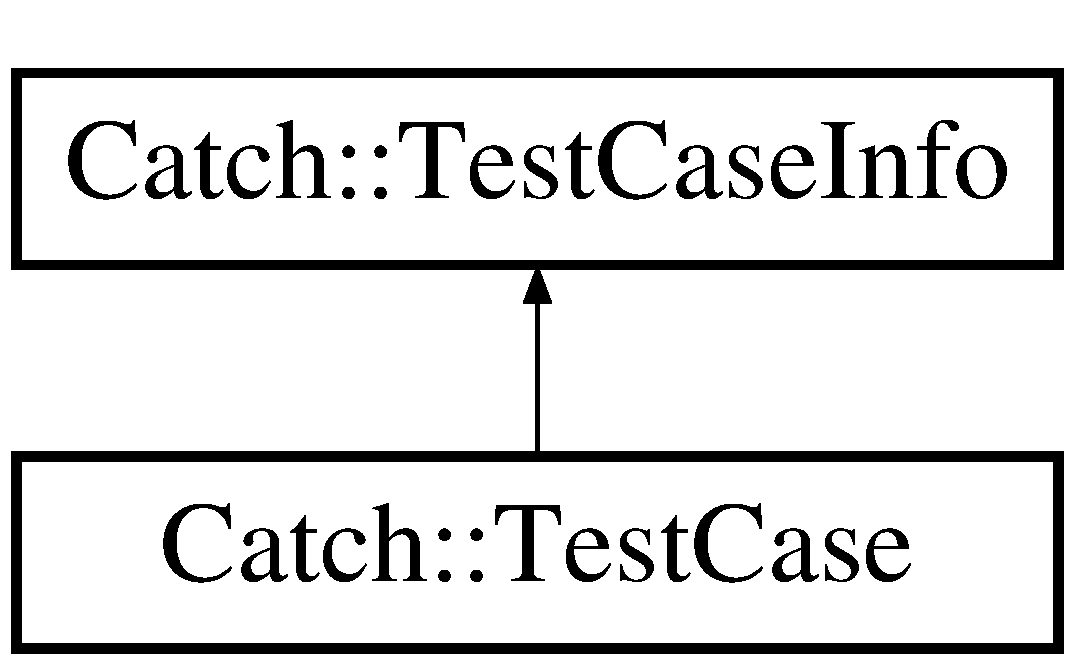
\includegraphics[height=2.000000cm]{class_catch_1_1_test_case}
\end{center}
\end{figure}
\subsection*{Public Member Functions}
\begin{DoxyCompactItemize}
\item 
\mbox{\hyperlink{class_catch_1_1_test_case_a03a5b913484681bd6d398dc5e9c2a907}{Test\+Case}} (\mbox{\hyperlink{struct_catch_1_1_i_test_case}{I\+Test\+Case}} $\ast$test\+Case, \mbox{\hyperlink{struct_catch_1_1_test_case_info}{Test\+Case\+Info}} const \&info)
\item 
\mbox{\hyperlink{class_catch_1_1_test_case_ac0011d3789edc3e44edb41f13c4775a0}{Test\+Case}} (\mbox{\hyperlink{class_catch_1_1_test_case}{Test\+Case}} const \&other)
\item 
\mbox{\hyperlink{class_catch_1_1_test_case}{Test\+Case}} \mbox{\hyperlink{class_catch_1_1_test_case_a0812e8a216d09b087d5874687009f0d6}{with\+Name}} (std\+::string const \&\+\_\+new\+Name) const
\item 
void \mbox{\hyperlink{class_catch_1_1_test_case_a26f346c8446dded0562fe3818ae71651}{invoke}} () const
\item 
\mbox{\hyperlink{struct_catch_1_1_test_case_info}{Test\+Case\+Info}} const  \& \mbox{\hyperlink{class_catch_1_1_test_case_a1ea0d79f49156cebea076fe1ba50d2b6}{get\+Test\+Case\+Info}} () const
\item 
void \mbox{\hyperlink{class_catch_1_1_test_case_aee38f908faf10b905b209ca388275413}{swap}} (\mbox{\hyperlink{class_catch_1_1_test_case}{Test\+Case}} \&other)
\item 
bool \mbox{\hyperlink{class_catch_1_1_test_case_a5456d03a90f75292835c158f3a3374a1}{operator==}} (\mbox{\hyperlink{class_catch_1_1_test_case}{Test\+Case}} const \&other) const
\item 
bool \mbox{\hyperlink{class_catch_1_1_test_case_a030e4b9282e9b32e08c8bd5e5cd6fa98}{operator$<$}} (\mbox{\hyperlink{class_catch_1_1_test_case}{Test\+Case}} const \&other) const
\item 
\mbox{\hyperlink{class_catch_1_1_test_case}{Test\+Case}} \& \mbox{\hyperlink{class_catch_1_1_test_case_a8022e3f74232f7887d2d2cbbc8876502}{operator=}} (\mbox{\hyperlink{class_catch_1_1_test_case}{Test\+Case}} const \&other)
\end{DoxyCompactItemize}
\subsection*{Additional Inherited Members}


\subsection{Constructor \& Destructor Documentation}
\mbox{\Hypertarget{class_catch_1_1_test_case_a03a5b913484681bd6d398dc5e9c2a907}\label{class_catch_1_1_test_case_a03a5b913484681bd6d398dc5e9c2a907}} 
\index{Catch\+::\+Test\+Case@{Catch\+::\+Test\+Case}!Test\+Case@{Test\+Case}}
\index{Test\+Case@{Test\+Case}!Catch\+::\+Test\+Case@{Catch\+::\+Test\+Case}}
\subsubsection{\texorpdfstring{Test\+Case()}{TestCase()}\hspace{0.1cm}{\footnotesize\ttfamily [1/2]}}
{\footnotesize\ttfamily Catch\+::\+Test\+Case\+::\+Test\+Case (\begin{DoxyParamCaption}\item[{\mbox{\hyperlink{struct_catch_1_1_i_test_case}{I\+Test\+Case}} $\ast$}]{test\+Case,  }\item[{\mbox{\hyperlink{struct_catch_1_1_test_case_info}{Test\+Case\+Info}} const \&}]{info }\end{DoxyParamCaption})}

\mbox{\Hypertarget{class_catch_1_1_test_case_ac0011d3789edc3e44edb41f13c4775a0}\label{class_catch_1_1_test_case_ac0011d3789edc3e44edb41f13c4775a0}} 
\index{Catch\+::\+Test\+Case@{Catch\+::\+Test\+Case}!Test\+Case@{Test\+Case}}
\index{Test\+Case@{Test\+Case}!Catch\+::\+Test\+Case@{Catch\+::\+Test\+Case}}
\subsubsection{\texorpdfstring{Test\+Case()}{TestCase()}\hspace{0.1cm}{\footnotesize\ttfamily [2/2]}}
{\footnotesize\ttfamily Catch\+::\+Test\+Case\+::\+Test\+Case (\begin{DoxyParamCaption}\item[{\mbox{\hyperlink{class_catch_1_1_test_case}{Test\+Case}} const \&}]{other }\end{DoxyParamCaption})}



\subsection{Member Function Documentation}
\mbox{\Hypertarget{class_catch_1_1_test_case_a1ea0d79f49156cebea076fe1ba50d2b6}\label{class_catch_1_1_test_case_a1ea0d79f49156cebea076fe1ba50d2b6}} 
\index{Catch\+::\+Test\+Case@{Catch\+::\+Test\+Case}!get\+Test\+Case\+Info@{get\+Test\+Case\+Info}}
\index{get\+Test\+Case\+Info@{get\+Test\+Case\+Info}!Catch\+::\+Test\+Case@{Catch\+::\+Test\+Case}}
\subsubsection{\texorpdfstring{get\+Test\+Case\+Info()}{getTestCaseInfo()}}
{\footnotesize\ttfamily \mbox{\hyperlink{struct_catch_1_1_test_case_info}{Test\+Case\+Info}} const\& Catch\+::\+Test\+Case\+::get\+Test\+Case\+Info (\begin{DoxyParamCaption}{ }\end{DoxyParamCaption}) const}

\mbox{\Hypertarget{class_catch_1_1_test_case_a26f346c8446dded0562fe3818ae71651}\label{class_catch_1_1_test_case_a26f346c8446dded0562fe3818ae71651}} 
\index{Catch\+::\+Test\+Case@{Catch\+::\+Test\+Case}!invoke@{invoke}}
\index{invoke@{invoke}!Catch\+::\+Test\+Case@{Catch\+::\+Test\+Case}}
\subsubsection{\texorpdfstring{invoke()}{invoke()}}
{\footnotesize\ttfamily void Catch\+::\+Test\+Case\+::invoke (\begin{DoxyParamCaption}{ }\end{DoxyParamCaption}) const}

\mbox{\Hypertarget{class_catch_1_1_test_case_a030e4b9282e9b32e08c8bd5e5cd6fa98}\label{class_catch_1_1_test_case_a030e4b9282e9b32e08c8bd5e5cd6fa98}} 
\index{Catch\+::\+Test\+Case@{Catch\+::\+Test\+Case}!operator$<$@{operator$<$}}
\index{operator$<$@{operator$<$}!Catch\+::\+Test\+Case@{Catch\+::\+Test\+Case}}
\subsubsection{\texorpdfstring{operator$<$()}{operator<()}}
{\footnotesize\ttfamily bool Catch\+::\+Test\+Case\+::operator$<$ (\begin{DoxyParamCaption}\item[{\mbox{\hyperlink{class_catch_1_1_test_case}{Test\+Case}} const \&}]{other }\end{DoxyParamCaption}) const}

\mbox{\Hypertarget{class_catch_1_1_test_case_a8022e3f74232f7887d2d2cbbc8876502}\label{class_catch_1_1_test_case_a8022e3f74232f7887d2d2cbbc8876502}} 
\index{Catch\+::\+Test\+Case@{Catch\+::\+Test\+Case}!operator=@{operator=}}
\index{operator=@{operator=}!Catch\+::\+Test\+Case@{Catch\+::\+Test\+Case}}
\subsubsection{\texorpdfstring{operator=()}{operator=()}}
{\footnotesize\ttfamily \mbox{\hyperlink{class_catch_1_1_test_case}{Test\+Case}}\& Catch\+::\+Test\+Case\+::operator= (\begin{DoxyParamCaption}\item[{\mbox{\hyperlink{class_catch_1_1_test_case}{Test\+Case}} const \&}]{other }\end{DoxyParamCaption})}

\mbox{\Hypertarget{class_catch_1_1_test_case_a5456d03a90f75292835c158f3a3374a1}\label{class_catch_1_1_test_case_a5456d03a90f75292835c158f3a3374a1}} 
\index{Catch\+::\+Test\+Case@{Catch\+::\+Test\+Case}!operator==@{operator==}}
\index{operator==@{operator==}!Catch\+::\+Test\+Case@{Catch\+::\+Test\+Case}}
\subsubsection{\texorpdfstring{operator==()}{operator==()}}
{\footnotesize\ttfamily bool Catch\+::\+Test\+Case\+::operator== (\begin{DoxyParamCaption}\item[{\mbox{\hyperlink{class_catch_1_1_test_case}{Test\+Case}} const \&}]{other }\end{DoxyParamCaption}) const}

\mbox{\Hypertarget{class_catch_1_1_test_case_aee38f908faf10b905b209ca388275413}\label{class_catch_1_1_test_case_aee38f908faf10b905b209ca388275413}} 
\index{Catch\+::\+Test\+Case@{Catch\+::\+Test\+Case}!swap@{swap}}
\index{swap@{swap}!Catch\+::\+Test\+Case@{Catch\+::\+Test\+Case}}
\subsubsection{\texorpdfstring{swap()}{swap()}}
{\footnotesize\ttfamily void Catch\+::\+Test\+Case\+::swap (\begin{DoxyParamCaption}\item[{\mbox{\hyperlink{class_catch_1_1_test_case}{Test\+Case}} \&}]{other }\end{DoxyParamCaption})}

\mbox{\Hypertarget{class_catch_1_1_test_case_a0812e8a216d09b087d5874687009f0d6}\label{class_catch_1_1_test_case_a0812e8a216d09b087d5874687009f0d6}} 
\index{Catch\+::\+Test\+Case@{Catch\+::\+Test\+Case}!with\+Name@{with\+Name}}
\index{with\+Name@{with\+Name}!Catch\+::\+Test\+Case@{Catch\+::\+Test\+Case}}
\subsubsection{\texorpdfstring{with\+Name()}{withName()}}
{\footnotesize\ttfamily \mbox{\hyperlink{class_catch_1_1_test_case}{Test\+Case}} Catch\+::\+Test\+Case\+::with\+Name (\begin{DoxyParamCaption}\item[{std\+::string const \&}]{\+\_\+new\+Name }\end{DoxyParamCaption}) const}



The documentation for this class was generated from the following file\+:\begin{DoxyCompactItemize}
\item 
include/\mbox{\hyperlink{catch_8hpp}{catch.\+hpp}}\end{DoxyCompactItemize}

\hypertarget{struct_catch_1_1_test_case_info}{}\section{Catch\+:\+:Test\+Case\+Info Struct Reference}
\label{struct_catch_1_1_test_case_info}\index{Catch\+::\+Test\+Case\+Info@{Catch\+::\+Test\+Case\+Info}}


{\ttfamily \#include $<$catch.\+hpp$>$}

Inheritance diagram for Catch\+:\+:Test\+Case\+Info\+:\begin{figure}[H]
\begin{center}
\leavevmode
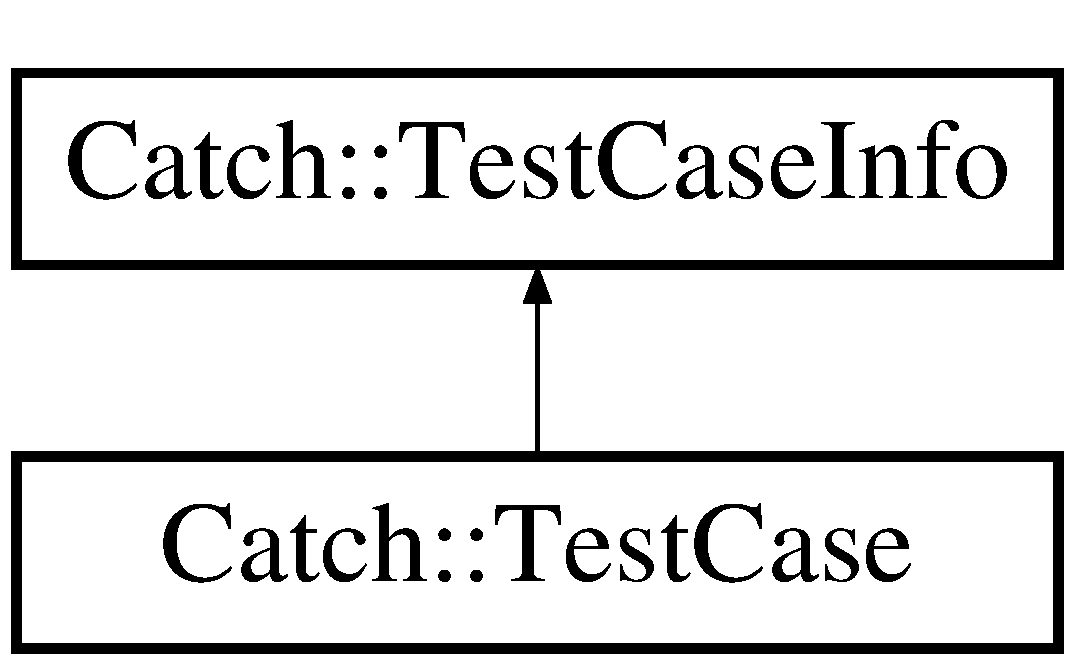
\includegraphics[height=2.000000cm]{struct_catch_1_1_test_case_info}
\end{center}
\end{figure}
\subsection*{Public Types}
\begin{DoxyCompactItemize}
\item 
enum \mbox{\hyperlink{struct_catch_1_1_test_case_info_a39b232f74b4a7a6f2183b96759027eac}{Special\+Properties}} \{ \newline
\mbox{\hyperlink{struct_catch_1_1_test_case_info_a39b232f74b4a7a6f2183b96759027eacaf94e9de5f8ec1e53b1aa761ec564b31a}{None}} = 0, 
\mbox{\hyperlink{struct_catch_1_1_test_case_info_a39b232f74b4a7a6f2183b96759027eacaeda53906c14c3973e0980900c132b8f7}{Is\+Hidden}} = 1 $<$$<$ 1, 
\mbox{\hyperlink{struct_catch_1_1_test_case_info_a39b232f74b4a7a6f2183b96759027eacaf9002285bccfc343935958f3953f4c01}{Should\+Fail}} = 1 $<$$<$ 2, 
\mbox{\hyperlink{struct_catch_1_1_test_case_info_a39b232f74b4a7a6f2183b96759027eacadf1873d3271121cb9f52d7df45b416ca}{May\+Fail}} = 1 $<$$<$ 3, 
\newline
\mbox{\hyperlink{struct_catch_1_1_test_case_info_a39b232f74b4a7a6f2183b96759027eaca4704adf89ed7f7ad653d08f99813a974}{Throws}} = 1 $<$$<$ 4, 
\mbox{\hyperlink{struct_catch_1_1_test_case_info_a39b232f74b4a7a6f2183b96759027eaca06472887b53fda9eb8015d74e7fd2cf1}{Non\+Portable}} = 1 $<$$<$ 5
 \}
\end{DoxyCompactItemize}
\subsection*{Public Member Functions}
\begin{DoxyCompactItemize}
\item 
\mbox{\hyperlink{struct_catch_1_1_test_case_info_a35ec65315e0d1f178491b5a59f3f3123}{Test\+Case\+Info}} (std\+::string const \&\+\_\+name, std\+::string const \&\+\_\+class\+Name, std\+::string const \&\+\_\+description, std\+::set$<$ std\+::string $>$ const \&\+\_\+tags, \mbox{\hyperlink{struct_catch_1_1_source_line_info}{Source\+Line\+Info}} const \&\+\_\+line\+Info)
\item 
\mbox{\hyperlink{struct_catch_1_1_test_case_info_ac338adb4e38f4bf3977fb45b2b1fe447}{Test\+Case\+Info}} (\mbox{\hyperlink{struct_catch_1_1_test_case_info}{Test\+Case\+Info}} const \&other)
\item 
bool \mbox{\hyperlink{struct_catch_1_1_test_case_info_a934b1a0952700743e99d62ec1731a2e2}{is\+Hidden}} () const
\item 
bool \mbox{\hyperlink{struct_catch_1_1_test_case_info_afc70d4379a2070cc22b693ffe3932c1a}{throws}} () const
\item 
bool \mbox{\hyperlink{struct_catch_1_1_test_case_info_a5f37291295e3a6de2dd85324c941edaf}{ok\+To\+Fail}} () const
\item 
bool \mbox{\hyperlink{struct_catch_1_1_test_case_info_abe33d81233230cdae8afa714688e905b}{expected\+To\+Fail}} () const
\end{DoxyCompactItemize}
\subsection*{Public Attributes}
\begin{DoxyCompactItemize}
\item 
std\+::string \mbox{\hyperlink{struct_catch_1_1_test_case_info_a463794e2f5cfead307c93efd134ade36}{name}}
\item 
std\+::string \mbox{\hyperlink{struct_catch_1_1_test_case_info_a1a5e0825132a38d091defdebbf2f8ce9}{class\+Name}}
\item 
std\+::string \mbox{\hyperlink{struct_catch_1_1_test_case_info_a37fe2db9425bc45f6a33893eac31198e}{description}}
\item 
std\+::set$<$ std\+::string $>$ \mbox{\hyperlink{struct_catch_1_1_test_case_info_a045f62e7719a8760a5b456f7fd2dc97c}{tags}}
\item 
std\+::set$<$ std\+::string $>$ \mbox{\hyperlink{struct_catch_1_1_test_case_info_a0ed3864a313e8ddc3ae38431be5be9ae}{lcase\+Tags}}
\item 
std\+::string \mbox{\hyperlink{struct_catch_1_1_test_case_info_ac65c2d36fd36f71e9bf782b2ea245c64}{tags\+As\+String}}
\item 
\mbox{\hyperlink{struct_catch_1_1_source_line_info}{Source\+Line\+Info}} \mbox{\hyperlink{struct_catch_1_1_test_case_info_aa9407b7f442655b51a2aad24b3fa2fd3}{line\+Info}}
\item 
\mbox{\hyperlink{struct_catch_1_1_test_case_info_a39b232f74b4a7a6f2183b96759027eac}{Special\+Properties}} \mbox{\hyperlink{struct_catch_1_1_test_case_info_afc1e84bd7a2e180895a06d9131302af0}{properties}}
\end{DoxyCompactItemize}
\subsection*{Friends}
\begin{DoxyCompactItemize}
\item 
void \mbox{\hyperlink{struct_catch_1_1_test_case_info_addc10c770e56f49da5baa0c76cf25bd5}{set\+Tags}} (\mbox{\hyperlink{struct_catch_1_1_test_case_info}{Test\+Case\+Info}} \&test\+Case\+Info, std\+::set$<$ std\+::string $>$ const \&\mbox{\hyperlink{struct_catch_1_1_test_case_info_a045f62e7719a8760a5b456f7fd2dc97c}{tags}})
\end{DoxyCompactItemize}


\subsection{Member Enumeration Documentation}
\mbox{\Hypertarget{struct_catch_1_1_test_case_info_a39b232f74b4a7a6f2183b96759027eac}\label{struct_catch_1_1_test_case_info_a39b232f74b4a7a6f2183b96759027eac}} 
\index{Catch\+::\+Test\+Case\+Info@{Catch\+::\+Test\+Case\+Info}!Special\+Properties@{Special\+Properties}}
\index{Special\+Properties@{Special\+Properties}!Catch\+::\+Test\+Case\+Info@{Catch\+::\+Test\+Case\+Info}}
\subsubsection{\texorpdfstring{Special\+Properties}{SpecialProperties}}
{\footnotesize\ttfamily enum \mbox{\hyperlink{struct_catch_1_1_test_case_info_a39b232f74b4a7a6f2183b96759027eac}{Catch\+::\+Test\+Case\+Info\+::\+Special\+Properties}}}

\begin{DoxyEnumFields}{Enumerator}
\raisebox{\heightof{T}}[0pt][0pt]{\index{None@{None}!Catch\+::\+Test\+Case\+Info@{Catch\+::\+Test\+Case\+Info}}\index{Catch\+::\+Test\+Case\+Info@{Catch\+::\+Test\+Case\+Info}!None@{None}}}\mbox{\Hypertarget{struct_catch_1_1_test_case_info_a39b232f74b4a7a6f2183b96759027eacaf94e9de5f8ec1e53b1aa761ec564b31a}\label{struct_catch_1_1_test_case_info_a39b232f74b4a7a6f2183b96759027eacaf94e9de5f8ec1e53b1aa761ec564b31a}} 
None&\\
\hline

\raisebox{\heightof{T}}[0pt][0pt]{\index{Is\+Hidden@{Is\+Hidden}!Catch\+::\+Test\+Case\+Info@{Catch\+::\+Test\+Case\+Info}}\index{Catch\+::\+Test\+Case\+Info@{Catch\+::\+Test\+Case\+Info}!Is\+Hidden@{Is\+Hidden}}}\mbox{\Hypertarget{struct_catch_1_1_test_case_info_a39b232f74b4a7a6f2183b96759027eacaeda53906c14c3973e0980900c132b8f7}\label{struct_catch_1_1_test_case_info_a39b232f74b4a7a6f2183b96759027eacaeda53906c14c3973e0980900c132b8f7}} 
Is\+Hidden&\\
\hline

\raisebox{\heightof{T}}[0pt][0pt]{\index{Should\+Fail@{Should\+Fail}!Catch\+::\+Test\+Case\+Info@{Catch\+::\+Test\+Case\+Info}}\index{Catch\+::\+Test\+Case\+Info@{Catch\+::\+Test\+Case\+Info}!Should\+Fail@{Should\+Fail}}}\mbox{\Hypertarget{struct_catch_1_1_test_case_info_a39b232f74b4a7a6f2183b96759027eacaf9002285bccfc343935958f3953f4c01}\label{struct_catch_1_1_test_case_info_a39b232f74b4a7a6f2183b96759027eacaf9002285bccfc343935958f3953f4c01}} 
Should\+Fail&\\
\hline

\raisebox{\heightof{T}}[0pt][0pt]{\index{May\+Fail@{May\+Fail}!Catch\+::\+Test\+Case\+Info@{Catch\+::\+Test\+Case\+Info}}\index{Catch\+::\+Test\+Case\+Info@{Catch\+::\+Test\+Case\+Info}!May\+Fail@{May\+Fail}}}\mbox{\Hypertarget{struct_catch_1_1_test_case_info_a39b232f74b4a7a6f2183b96759027eacadf1873d3271121cb9f52d7df45b416ca}\label{struct_catch_1_1_test_case_info_a39b232f74b4a7a6f2183b96759027eacadf1873d3271121cb9f52d7df45b416ca}} 
May\+Fail&\\
\hline

\raisebox{\heightof{T}}[0pt][0pt]{\index{Throws@{Throws}!Catch\+::\+Test\+Case\+Info@{Catch\+::\+Test\+Case\+Info}}\index{Catch\+::\+Test\+Case\+Info@{Catch\+::\+Test\+Case\+Info}!Throws@{Throws}}}\mbox{\Hypertarget{struct_catch_1_1_test_case_info_a39b232f74b4a7a6f2183b96759027eaca4704adf89ed7f7ad653d08f99813a974}\label{struct_catch_1_1_test_case_info_a39b232f74b4a7a6f2183b96759027eaca4704adf89ed7f7ad653d08f99813a974}} 
Throws&\\
\hline

\raisebox{\heightof{T}}[0pt][0pt]{\index{Non\+Portable@{Non\+Portable}!Catch\+::\+Test\+Case\+Info@{Catch\+::\+Test\+Case\+Info}}\index{Catch\+::\+Test\+Case\+Info@{Catch\+::\+Test\+Case\+Info}!Non\+Portable@{Non\+Portable}}}\mbox{\Hypertarget{struct_catch_1_1_test_case_info_a39b232f74b4a7a6f2183b96759027eaca06472887b53fda9eb8015d74e7fd2cf1}\label{struct_catch_1_1_test_case_info_a39b232f74b4a7a6f2183b96759027eaca06472887b53fda9eb8015d74e7fd2cf1}} 
Non\+Portable&\\
\hline

\end{DoxyEnumFields}


\subsection{Constructor \& Destructor Documentation}
\mbox{\Hypertarget{struct_catch_1_1_test_case_info_a35ec65315e0d1f178491b5a59f3f3123}\label{struct_catch_1_1_test_case_info_a35ec65315e0d1f178491b5a59f3f3123}} 
\index{Catch\+::\+Test\+Case\+Info@{Catch\+::\+Test\+Case\+Info}!Test\+Case\+Info@{Test\+Case\+Info}}
\index{Test\+Case\+Info@{Test\+Case\+Info}!Catch\+::\+Test\+Case\+Info@{Catch\+::\+Test\+Case\+Info}}
\subsubsection{\texorpdfstring{Test\+Case\+Info()}{TestCaseInfo()}\hspace{0.1cm}{\footnotesize\ttfamily [1/2]}}
{\footnotesize\ttfamily Catch\+::\+Test\+Case\+Info\+::\+Test\+Case\+Info (\begin{DoxyParamCaption}\item[{std\+::string const \&}]{\+\_\+name,  }\item[{std\+::string const \&}]{\+\_\+class\+Name,  }\item[{std\+::string const \&}]{\+\_\+description,  }\item[{std\+::set$<$ std\+::string $>$ const \&}]{\+\_\+tags,  }\item[{\mbox{\hyperlink{struct_catch_1_1_source_line_info}{Source\+Line\+Info}} const \&}]{\+\_\+line\+Info }\end{DoxyParamCaption})}

\mbox{\Hypertarget{struct_catch_1_1_test_case_info_ac338adb4e38f4bf3977fb45b2b1fe447}\label{struct_catch_1_1_test_case_info_ac338adb4e38f4bf3977fb45b2b1fe447}} 
\index{Catch\+::\+Test\+Case\+Info@{Catch\+::\+Test\+Case\+Info}!Test\+Case\+Info@{Test\+Case\+Info}}
\index{Test\+Case\+Info@{Test\+Case\+Info}!Catch\+::\+Test\+Case\+Info@{Catch\+::\+Test\+Case\+Info}}
\subsubsection{\texorpdfstring{Test\+Case\+Info()}{TestCaseInfo()}\hspace{0.1cm}{\footnotesize\ttfamily [2/2]}}
{\footnotesize\ttfamily Catch\+::\+Test\+Case\+Info\+::\+Test\+Case\+Info (\begin{DoxyParamCaption}\item[{\mbox{\hyperlink{struct_catch_1_1_test_case_info}{Test\+Case\+Info}} const \&}]{other }\end{DoxyParamCaption})}



\subsection{Member Function Documentation}
\mbox{\Hypertarget{struct_catch_1_1_test_case_info_abe33d81233230cdae8afa714688e905b}\label{struct_catch_1_1_test_case_info_abe33d81233230cdae8afa714688e905b}} 
\index{Catch\+::\+Test\+Case\+Info@{Catch\+::\+Test\+Case\+Info}!expected\+To\+Fail@{expected\+To\+Fail}}
\index{expected\+To\+Fail@{expected\+To\+Fail}!Catch\+::\+Test\+Case\+Info@{Catch\+::\+Test\+Case\+Info}}
\subsubsection{\texorpdfstring{expected\+To\+Fail()}{expectedToFail()}}
{\footnotesize\ttfamily bool Catch\+::\+Test\+Case\+Info\+::expected\+To\+Fail (\begin{DoxyParamCaption}{ }\end{DoxyParamCaption}) const}

\mbox{\Hypertarget{struct_catch_1_1_test_case_info_a934b1a0952700743e99d62ec1731a2e2}\label{struct_catch_1_1_test_case_info_a934b1a0952700743e99d62ec1731a2e2}} 
\index{Catch\+::\+Test\+Case\+Info@{Catch\+::\+Test\+Case\+Info}!is\+Hidden@{is\+Hidden}}
\index{is\+Hidden@{is\+Hidden}!Catch\+::\+Test\+Case\+Info@{Catch\+::\+Test\+Case\+Info}}
\subsubsection{\texorpdfstring{is\+Hidden()}{isHidden()}}
{\footnotesize\ttfamily bool Catch\+::\+Test\+Case\+Info\+::is\+Hidden (\begin{DoxyParamCaption}{ }\end{DoxyParamCaption}) const}

\mbox{\Hypertarget{struct_catch_1_1_test_case_info_a5f37291295e3a6de2dd85324c941edaf}\label{struct_catch_1_1_test_case_info_a5f37291295e3a6de2dd85324c941edaf}} 
\index{Catch\+::\+Test\+Case\+Info@{Catch\+::\+Test\+Case\+Info}!ok\+To\+Fail@{ok\+To\+Fail}}
\index{ok\+To\+Fail@{ok\+To\+Fail}!Catch\+::\+Test\+Case\+Info@{Catch\+::\+Test\+Case\+Info}}
\subsubsection{\texorpdfstring{ok\+To\+Fail()}{okToFail()}}
{\footnotesize\ttfamily bool Catch\+::\+Test\+Case\+Info\+::ok\+To\+Fail (\begin{DoxyParamCaption}{ }\end{DoxyParamCaption}) const}

\mbox{\Hypertarget{struct_catch_1_1_test_case_info_afc70d4379a2070cc22b693ffe3932c1a}\label{struct_catch_1_1_test_case_info_afc70d4379a2070cc22b693ffe3932c1a}} 
\index{Catch\+::\+Test\+Case\+Info@{Catch\+::\+Test\+Case\+Info}!throws@{throws}}
\index{throws@{throws}!Catch\+::\+Test\+Case\+Info@{Catch\+::\+Test\+Case\+Info}}
\subsubsection{\texorpdfstring{throws()}{throws()}}
{\footnotesize\ttfamily bool Catch\+::\+Test\+Case\+Info\+::throws (\begin{DoxyParamCaption}{ }\end{DoxyParamCaption}) const}



\subsection{Friends And Related Function Documentation}
\mbox{\Hypertarget{struct_catch_1_1_test_case_info_addc10c770e56f49da5baa0c76cf25bd5}\label{struct_catch_1_1_test_case_info_addc10c770e56f49da5baa0c76cf25bd5}} 
\index{Catch\+::\+Test\+Case\+Info@{Catch\+::\+Test\+Case\+Info}!set\+Tags@{set\+Tags}}
\index{set\+Tags@{set\+Tags}!Catch\+::\+Test\+Case\+Info@{Catch\+::\+Test\+Case\+Info}}
\subsubsection{\texorpdfstring{set\+Tags}{setTags}}
{\footnotesize\ttfamily void set\+Tags (\begin{DoxyParamCaption}\item[{\mbox{\hyperlink{struct_catch_1_1_test_case_info}{Test\+Case\+Info}} \&}]{test\+Case\+Info,  }\item[{std\+::set$<$ std\+::string $>$ const \&}]{tags }\end{DoxyParamCaption})\hspace{0.3cm}{\ttfamily [friend]}}



\subsection{Member Data Documentation}
\mbox{\Hypertarget{struct_catch_1_1_test_case_info_a1a5e0825132a38d091defdebbf2f8ce9}\label{struct_catch_1_1_test_case_info_a1a5e0825132a38d091defdebbf2f8ce9}} 
\index{Catch\+::\+Test\+Case\+Info@{Catch\+::\+Test\+Case\+Info}!class\+Name@{class\+Name}}
\index{class\+Name@{class\+Name}!Catch\+::\+Test\+Case\+Info@{Catch\+::\+Test\+Case\+Info}}
\subsubsection{\texorpdfstring{class\+Name}{className}}
{\footnotesize\ttfamily std\+::string Catch\+::\+Test\+Case\+Info\+::class\+Name}

\mbox{\Hypertarget{struct_catch_1_1_test_case_info_a37fe2db9425bc45f6a33893eac31198e}\label{struct_catch_1_1_test_case_info_a37fe2db9425bc45f6a33893eac31198e}} 
\index{Catch\+::\+Test\+Case\+Info@{Catch\+::\+Test\+Case\+Info}!description@{description}}
\index{description@{description}!Catch\+::\+Test\+Case\+Info@{Catch\+::\+Test\+Case\+Info}}
\subsubsection{\texorpdfstring{description}{description}}
{\footnotesize\ttfamily std\+::string Catch\+::\+Test\+Case\+Info\+::description}

\mbox{\Hypertarget{struct_catch_1_1_test_case_info_a0ed3864a313e8ddc3ae38431be5be9ae}\label{struct_catch_1_1_test_case_info_a0ed3864a313e8ddc3ae38431be5be9ae}} 
\index{Catch\+::\+Test\+Case\+Info@{Catch\+::\+Test\+Case\+Info}!lcase\+Tags@{lcase\+Tags}}
\index{lcase\+Tags@{lcase\+Tags}!Catch\+::\+Test\+Case\+Info@{Catch\+::\+Test\+Case\+Info}}
\subsubsection{\texorpdfstring{lcase\+Tags}{lcaseTags}}
{\footnotesize\ttfamily std\+::set$<$std\+::string$>$ Catch\+::\+Test\+Case\+Info\+::lcase\+Tags}

\mbox{\Hypertarget{struct_catch_1_1_test_case_info_aa9407b7f442655b51a2aad24b3fa2fd3}\label{struct_catch_1_1_test_case_info_aa9407b7f442655b51a2aad24b3fa2fd3}} 
\index{Catch\+::\+Test\+Case\+Info@{Catch\+::\+Test\+Case\+Info}!line\+Info@{line\+Info}}
\index{line\+Info@{line\+Info}!Catch\+::\+Test\+Case\+Info@{Catch\+::\+Test\+Case\+Info}}
\subsubsection{\texorpdfstring{line\+Info}{lineInfo}}
{\footnotesize\ttfamily \mbox{\hyperlink{struct_catch_1_1_source_line_info}{Source\+Line\+Info}} Catch\+::\+Test\+Case\+Info\+::line\+Info}

\mbox{\Hypertarget{struct_catch_1_1_test_case_info_a463794e2f5cfead307c93efd134ade36}\label{struct_catch_1_1_test_case_info_a463794e2f5cfead307c93efd134ade36}} 
\index{Catch\+::\+Test\+Case\+Info@{Catch\+::\+Test\+Case\+Info}!name@{name}}
\index{name@{name}!Catch\+::\+Test\+Case\+Info@{Catch\+::\+Test\+Case\+Info}}
\subsubsection{\texorpdfstring{name}{name}}
{\footnotesize\ttfamily std\+::string Catch\+::\+Test\+Case\+Info\+::name}

\mbox{\Hypertarget{struct_catch_1_1_test_case_info_afc1e84bd7a2e180895a06d9131302af0}\label{struct_catch_1_1_test_case_info_afc1e84bd7a2e180895a06d9131302af0}} 
\index{Catch\+::\+Test\+Case\+Info@{Catch\+::\+Test\+Case\+Info}!properties@{properties}}
\index{properties@{properties}!Catch\+::\+Test\+Case\+Info@{Catch\+::\+Test\+Case\+Info}}
\subsubsection{\texorpdfstring{properties}{properties}}
{\footnotesize\ttfamily \mbox{\hyperlink{struct_catch_1_1_test_case_info_a39b232f74b4a7a6f2183b96759027eac}{Special\+Properties}} Catch\+::\+Test\+Case\+Info\+::properties}

\mbox{\Hypertarget{struct_catch_1_1_test_case_info_a045f62e7719a8760a5b456f7fd2dc97c}\label{struct_catch_1_1_test_case_info_a045f62e7719a8760a5b456f7fd2dc97c}} 
\index{Catch\+::\+Test\+Case\+Info@{Catch\+::\+Test\+Case\+Info}!tags@{tags}}
\index{tags@{tags}!Catch\+::\+Test\+Case\+Info@{Catch\+::\+Test\+Case\+Info}}
\subsubsection{\texorpdfstring{tags}{tags}}
{\footnotesize\ttfamily std\+::set$<$std\+::string$>$ Catch\+::\+Test\+Case\+Info\+::tags}

\mbox{\Hypertarget{struct_catch_1_1_test_case_info_ac65c2d36fd36f71e9bf782b2ea245c64}\label{struct_catch_1_1_test_case_info_ac65c2d36fd36f71e9bf782b2ea245c64}} 
\index{Catch\+::\+Test\+Case\+Info@{Catch\+::\+Test\+Case\+Info}!tags\+As\+String@{tags\+As\+String}}
\index{tags\+As\+String@{tags\+As\+String}!Catch\+::\+Test\+Case\+Info@{Catch\+::\+Test\+Case\+Info}}
\subsubsection{\texorpdfstring{tags\+As\+String}{tagsAsString}}
{\footnotesize\ttfamily std\+::string Catch\+::\+Test\+Case\+Info\+::tags\+As\+String}



The documentation for this struct was generated from the following file\+:\begin{DoxyCompactItemize}
\item 
include/\mbox{\hyperlink{catch_8hpp}{catch.\+hpp}}\end{DoxyCompactItemize}

\hypertarget{struct_catch_1_1_test_failure_exception}{}\section{Catch\+:\+:Test\+Failure\+Exception Struct Reference}
\label{struct_catch_1_1_test_failure_exception}\index{Catch\+::\+Test\+Failure\+Exception@{Catch\+::\+Test\+Failure\+Exception}}


{\ttfamily \#include $<$catch.\+hpp$>$}



The documentation for this struct was generated from the following file\+:\begin{DoxyCompactItemize}
\item 
include/\mbox{\hyperlink{catch_8hpp}{catch.\+hpp}}\end{DoxyCompactItemize}

\hypertarget{class_catch_1_1_timer}{}\section{Catch\+:\+:Timer Class Reference}
\label{class_catch_1_1_timer}\index{Catch\+::\+Timer@{Catch\+::\+Timer}}


{\ttfamily \#include $<$catch.\+hpp$>$}

\subsection*{Public Member Functions}
\begin{DoxyCompactItemize}
\item 
\mbox{\hyperlink{class_catch_1_1_timer_af09b7cd7a40af71f4704262afb31558a}{Timer}} ()
\item 
void \mbox{\hyperlink{class_catch_1_1_timer_a0a56e879e43f36c102bf9ea8b5fc8b72}{start}} ()
\item 
unsigned int \mbox{\hyperlink{class_catch_1_1_timer_af592ca4a9d340b9855732e4af777eaf0}{get\+Elapsed\+Microseconds}} () const
\item 
unsigned int \mbox{\hyperlink{class_catch_1_1_timer_a2081b2d36950ab6912e7c4958afe0099}{get\+Elapsed\+Milliseconds}} () const
\item 
double \mbox{\hyperlink{class_catch_1_1_timer_ae1615c8a9aa44b7a96cfe8a35d34e5de}{get\+Elapsed\+Seconds}} () const
\end{DoxyCompactItemize}


\subsection{Constructor \& Destructor Documentation}
\mbox{\Hypertarget{class_catch_1_1_timer_af09b7cd7a40af71f4704262afb31558a}\label{class_catch_1_1_timer_af09b7cd7a40af71f4704262afb31558a}} 
\index{Catch\+::\+Timer@{Catch\+::\+Timer}!Timer@{Timer}}
\index{Timer@{Timer}!Catch\+::\+Timer@{Catch\+::\+Timer}}
\subsubsection{\texorpdfstring{Timer()}{Timer()}}
{\footnotesize\ttfamily Catch\+::\+Timer\+::\+Timer (\begin{DoxyParamCaption}{ }\end{DoxyParamCaption})\hspace{0.3cm}{\ttfamily [inline]}}



\subsection{Member Function Documentation}
\mbox{\Hypertarget{class_catch_1_1_timer_af592ca4a9d340b9855732e4af777eaf0}\label{class_catch_1_1_timer_af592ca4a9d340b9855732e4af777eaf0}} 
\index{Catch\+::\+Timer@{Catch\+::\+Timer}!get\+Elapsed\+Microseconds@{get\+Elapsed\+Microseconds}}
\index{get\+Elapsed\+Microseconds@{get\+Elapsed\+Microseconds}!Catch\+::\+Timer@{Catch\+::\+Timer}}
\subsubsection{\texorpdfstring{get\+Elapsed\+Microseconds()}{getElapsedMicroseconds()}}
{\footnotesize\ttfamily unsigned int Catch\+::\+Timer\+::get\+Elapsed\+Microseconds (\begin{DoxyParamCaption}{ }\end{DoxyParamCaption}) const}

\mbox{\Hypertarget{class_catch_1_1_timer_a2081b2d36950ab6912e7c4958afe0099}\label{class_catch_1_1_timer_a2081b2d36950ab6912e7c4958afe0099}} 
\index{Catch\+::\+Timer@{Catch\+::\+Timer}!get\+Elapsed\+Milliseconds@{get\+Elapsed\+Milliseconds}}
\index{get\+Elapsed\+Milliseconds@{get\+Elapsed\+Milliseconds}!Catch\+::\+Timer@{Catch\+::\+Timer}}
\subsubsection{\texorpdfstring{get\+Elapsed\+Milliseconds()}{getElapsedMilliseconds()}}
{\footnotesize\ttfamily unsigned int Catch\+::\+Timer\+::get\+Elapsed\+Milliseconds (\begin{DoxyParamCaption}{ }\end{DoxyParamCaption}) const}

\mbox{\Hypertarget{class_catch_1_1_timer_ae1615c8a9aa44b7a96cfe8a35d34e5de}\label{class_catch_1_1_timer_ae1615c8a9aa44b7a96cfe8a35d34e5de}} 
\index{Catch\+::\+Timer@{Catch\+::\+Timer}!get\+Elapsed\+Seconds@{get\+Elapsed\+Seconds}}
\index{get\+Elapsed\+Seconds@{get\+Elapsed\+Seconds}!Catch\+::\+Timer@{Catch\+::\+Timer}}
\subsubsection{\texorpdfstring{get\+Elapsed\+Seconds()}{getElapsedSeconds()}}
{\footnotesize\ttfamily double Catch\+::\+Timer\+::get\+Elapsed\+Seconds (\begin{DoxyParamCaption}{ }\end{DoxyParamCaption}) const}

\mbox{\Hypertarget{class_catch_1_1_timer_a0a56e879e43f36c102bf9ea8b5fc8b72}\label{class_catch_1_1_timer_a0a56e879e43f36c102bf9ea8b5fc8b72}} 
\index{Catch\+::\+Timer@{Catch\+::\+Timer}!start@{start}}
\index{start@{start}!Catch\+::\+Timer@{Catch\+::\+Timer}}
\subsubsection{\texorpdfstring{start()}{start()}}
{\footnotesize\ttfamily void Catch\+::\+Timer\+::start (\begin{DoxyParamCaption}{ }\end{DoxyParamCaption})}



The documentation for this class was generated from the following file\+:\begin{DoxyCompactItemize}
\item 
include/\mbox{\hyperlink{catch_8hpp}{catch.\+hpp}}\end{DoxyCompactItemize}

\hypertarget{struct_catch_1_1_totals}{}\section{Catch\+:\+:Totals Struct Reference}
\label{struct_catch_1_1_totals}\index{Catch\+::\+Totals@{Catch\+::\+Totals}}


{\ttfamily \#include $<$catch.\+hpp$>$}

\subsection*{Public Member Functions}
\begin{DoxyCompactItemize}
\item 
\mbox{\hyperlink{struct_catch_1_1_totals}{Totals}} \mbox{\hyperlink{struct_catch_1_1_totals_a9279ed39139cb7e7b291918a6d08290e}{operator-\/}} (\mbox{\hyperlink{struct_catch_1_1_totals}{Totals}} const \&other) const
\item 
\mbox{\hyperlink{struct_catch_1_1_totals}{Totals}} \mbox{\hyperlink{struct_catch_1_1_totals_a1a94a654f5f3786b75695e081fc9bca2}{delta}} (\mbox{\hyperlink{struct_catch_1_1_totals}{Totals}} const \&prev\+Totals) const
\item 
\mbox{\hyperlink{struct_catch_1_1_totals}{Totals}} \& \mbox{\hyperlink{struct_catch_1_1_totals_a574015076e54cc405c70b053e3356e43}{operator+=}} (\mbox{\hyperlink{struct_catch_1_1_totals}{Totals}} const \&other)
\end{DoxyCompactItemize}
\subsection*{Public Attributes}
\begin{DoxyCompactItemize}
\item 
\mbox{\hyperlink{struct_catch_1_1_counts}{Counts}} \mbox{\hyperlink{struct_catch_1_1_totals_a885ded66df752147b30c3d45aa602ec9}{assertions}}
\item 
\mbox{\hyperlink{struct_catch_1_1_counts}{Counts}} \mbox{\hyperlink{struct_catch_1_1_totals_adb195fe477aedee2ecea88c888f16506}{test\+Cases}}
\end{DoxyCompactItemize}


\subsection{Member Function Documentation}
\mbox{\Hypertarget{struct_catch_1_1_totals_a1a94a654f5f3786b75695e081fc9bca2}\label{struct_catch_1_1_totals_a1a94a654f5f3786b75695e081fc9bca2}} 
\index{Catch\+::\+Totals@{Catch\+::\+Totals}!delta@{delta}}
\index{delta@{delta}!Catch\+::\+Totals@{Catch\+::\+Totals}}
\subsubsection{\texorpdfstring{delta()}{delta()}}
{\footnotesize\ttfamily \mbox{\hyperlink{struct_catch_1_1_totals}{Totals}} Catch\+::\+Totals\+::delta (\begin{DoxyParamCaption}\item[{\mbox{\hyperlink{struct_catch_1_1_totals}{Totals}} const \&}]{prev\+Totals }\end{DoxyParamCaption}) const\hspace{0.3cm}{\ttfamily [inline]}}

\mbox{\Hypertarget{struct_catch_1_1_totals_a574015076e54cc405c70b053e3356e43}\label{struct_catch_1_1_totals_a574015076e54cc405c70b053e3356e43}} 
\index{Catch\+::\+Totals@{Catch\+::\+Totals}!operator+=@{operator+=}}
\index{operator+=@{operator+=}!Catch\+::\+Totals@{Catch\+::\+Totals}}
\subsubsection{\texorpdfstring{operator+=()}{operator+=()}}
{\footnotesize\ttfamily \mbox{\hyperlink{struct_catch_1_1_totals}{Totals}}\& Catch\+::\+Totals\+::operator+= (\begin{DoxyParamCaption}\item[{\mbox{\hyperlink{struct_catch_1_1_totals}{Totals}} const \&}]{other }\end{DoxyParamCaption})\hspace{0.3cm}{\ttfamily [inline]}}

\mbox{\Hypertarget{struct_catch_1_1_totals_a9279ed39139cb7e7b291918a6d08290e}\label{struct_catch_1_1_totals_a9279ed39139cb7e7b291918a6d08290e}} 
\index{Catch\+::\+Totals@{Catch\+::\+Totals}!operator-\/@{operator-\/}}
\index{operator-\/@{operator-\/}!Catch\+::\+Totals@{Catch\+::\+Totals}}
\subsubsection{\texorpdfstring{operator-\/()}{operator-()}}
{\footnotesize\ttfamily \mbox{\hyperlink{struct_catch_1_1_totals}{Totals}} Catch\+::\+Totals\+::operator-\/ (\begin{DoxyParamCaption}\item[{\mbox{\hyperlink{struct_catch_1_1_totals}{Totals}} const \&}]{other }\end{DoxyParamCaption}) const\hspace{0.3cm}{\ttfamily [inline]}}



\subsection{Member Data Documentation}
\mbox{\Hypertarget{struct_catch_1_1_totals_a885ded66df752147b30c3d45aa602ec9}\label{struct_catch_1_1_totals_a885ded66df752147b30c3d45aa602ec9}} 
\index{Catch\+::\+Totals@{Catch\+::\+Totals}!assertions@{assertions}}
\index{assertions@{assertions}!Catch\+::\+Totals@{Catch\+::\+Totals}}
\subsubsection{\texorpdfstring{assertions}{assertions}}
{\footnotesize\ttfamily \mbox{\hyperlink{struct_catch_1_1_counts}{Counts}} Catch\+::\+Totals\+::assertions}

\mbox{\Hypertarget{struct_catch_1_1_totals_adb195fe477aedee2ecea88c888f16506}\label{struct_catch_1_1_totals_adb195fe477aedee2ecea88c888f16506}} 
\index{Catch\+::\+Totals@{Catch\+::\+Totals}!test\+Cases@{test\+Cases}}
\index{test\+Cases@{test\+Cases}!Catch\+::\+Totals@{Catch\+::\+Totals}}
\subsubsection{\texorpdfstring{test\+Cases}{testCases}}
{\footnotesize\ttfamily \mbox{\hyperlink{struct_catch_1_1_counts}{Counts}} Catch\+::\+Totals\+::test\+Cases}



The documentation for this struct was generated from the following file\+:\begin{DoxyCompactItemize}
\item 
include/\mbox{\hyperlink{catch_8hpp}{catch.\+hpp}}\end{DoxyCompactItemize}

\hypertarget{class_b_s_t_tree_1_1_tree}{}\section{B\+S\+T\+Tree\+:\+:Tree Class Reference}
\label{class_b_s_t_tree_1_1_tree}\index{B\+S\+T\+Tree\+::\+Tree@{B\+S\+T\+Tree\+::\+Tree}}


{\ttfamily \#include $<$tree.\+h$>$}

\subsection*{Public Member Functions}
\begin{DoxyCompactItemize}
\item 
\mbox{\hyperlink{class_b_s_t_tree_1_1_tree_ab341ae8f5ea3eec3dd7eb2acb0126e8b}{Tree}} ()
\item 
\mbox{\hyperlink{class_b_s_t_tree_1_1_tree_a425b43fb9301c18ac7241e173b05f7e0}{Tree}} (std\+::initializer\+\_\+list$<$ int $>$ list)
\item 
\mbox{\hyperlink{class_b_s_t_tree_1_1_tree_aa16db87e1a4e57addbbd8513f20150a5}{Tree}} (const \mbox{\hyperlink{class_b_s_t_tree_1_1_tree}{Tree}} \&tree)
\item 
\mbox{\hyperlink{class_b_s_t_tree_1_1_tree_a1177427abc9e4e1c77358c30b5eaeda2}{Tree}} (\mbox{\hyperlink{class_b_s_t_tree_1_1_tree}{Tree}} \&\&tree)
\item 
void \mbox{\hyperlink{class_b_s_t_tree_1_1_tree_a4f6816912547a485ab853eb125e261a2}{insert}} (int value)
\item 
void \mbox{\hyperlink{class_b_s_t_tree_1_1_tree_aaa4094ca75c834acc9dbd1201791450e}{print\+\_\+tree}} (int indent)
\item 
void \mbox{\hyperlink{class_b_s_t_tree_1_1_tree_a122d418f295da0b66ae050174e74a828}{show\+\_\+nodes}} (\mbox{\hyperlink{namespace_b_s_t_tree_a711723b85e5af09e10bfcc3a3b501fe2}{B\+S\+T\+Tree\+::traversal\+\_\+order}} order)
\item 
void \mbox{\hyperlink{class_b_s_t_tree_1_1_tree_ae1b302d3de2ca202f7b89bd46d4a7eca}{delete\+\_\+node}} (int value)
\item 
bool \mbox{\hyperlink{class_b_s_t_tree_1_1_tree_ac78c4c85e486aade23d8ac740a711537}{check\+\_\+existing}} (int key)
\item 
auto \mbox{\hyperlink{class_b_s_t_tree_1_1_tree_a4310f8ce5de32401811946bb20b5e634}{operator=}} (const \mbox{\hyperlink{class_b_s_t_tree_1_1_tree}{Tree}} \&tree) -\/$>$ \mbox{\hyperlink{class_b_s_t_tree_1_1_tree}{Tree}} \&
\item 
auto \mbox{\hyperlink{class_b_s_t_tree_1_1_tree_aa71187977d9e86293e250214bb53f423}{operator=}} (\mbox{\hyperlink{class_b_s_t_tree_1_1_tree}{Tree}} \&\&) -\/$>$ \mbox{\hyperlink{class_b_s_t_tree_1_1_tree}{Tree}} \&
\item 
\mbox{\hyperlink{class_b_s_t_tree_1_1_tree_a9342fe23d2476501afc8574ba822d0dd}{$\sim$\+Tree}} ()
\end{DoxyCompactItemize}
\subsection*{Friends}
\begin{DoxyCompactItemize}
\item 
auto \mbox{\hyperlink{class_b_s_t_tree_1_1_tree_a4df8fc028c7dd645f2d9507fcc0fa407}{operator$<$$<$}} (std\+::ostream \&stream, const \mbox{\hyperlink{class_b_s_t_tree_1_1_tree}{Tree}} \&tree) -\/$>$ std\+::ostream \&
\end{DoxyCompactItemize}


\subsection{Constructor \& Destructor Documentation}
\mbox{\Hypertarget{class_b_s_t_tree_1_1_tree_ab341ae8f5ea3eec3dd7eb2acb0126e8b}\label{class_b_s_t_tree_1_1_tree_ab341ae8f5ea3eec3dd7eb2acb0126e8b}} 
\index{B\+S\+T\+Tree\+::\+Tree@{B\+S\+T\+Tree\+::\+Tree}!Tree@{Tree}}
\index{Tree@{Tree}!B\+S\+T\+Tree\+::\+Tree@{B\+S\+T\+Tree\+::\+Tree}}
\subsubsection{\texorpdfstring{Tree()}{Tree()}\hspace{0.1cm}{\footnotesize\ttfamily [1/4]}}
{\footnotesize\ttfamily B\+S\+T\+Tree\+::\+Tree\+::\+Tree (\begin{DoxyParamCaption}{ }\end{DoxyParamCaption})}

стандартный конструктор \mbox{\Hypertarget{class_b_s_t_tree_1_1_tree_a425b43fb9301c18ac7241e173b05f7e0}\label{class_b_s_t_tree_1_1_tree_a425b43fb9301c18ac7241e173b05f7e0}} 
\index{B\+S\+T\+Tree\+::\+Tree@{B\+S\+T\+Tree\+::\+Tree}!Tree@{Tree}}
\index{Tree@{Tree}!B\+S\+T\+Tree\+::\+Tree@{B\+S\+T\+Tree\+::\+Tree}}
\subsubsection{\texorpdfstring{Tree()}{Tree()}\hspace{0.1cm}{\footnotesize\ttfamily [2/4]}}
{\footnotesize\ttfamily B\+S\+T\+Tree\+::\+Tree\+::\+Tree (\begin{DoxyParamCaption}\item[{std\+::initializer\+\_\+list$<$ int $>$}]{list }\end{DoxyParamCaption})}

конструктор из листа \mbox{\Hypertarget{class_b_s_t_tree_1_1_tree_aa16db87e1a4e57addbbd8513f20150a5}\label{class_b_s_t_tree_1_1_tree_aa16db87e1a4e57addbbd8513f20150a5}} 
\index{B\+S\+T\+Tree\+::\+Tree@{B\+S\+T\+Tree\+::\+Tree}!Tree@{Tree}}
\index{Tree@{Tree}!B\+S\+T\+Tree\+::\+Tree@{B\+S\+T\+Tree\+::\+Tree}}
\subsubsection{\texorpdfstring{Tree()}{Tree()}\hspace{0.1cm}{\footnotesize\ttfamily [3/4]}}
{\footnotesize\ttfamily B\+S\+T\+Tree\+::\+Tree\+::\+Tree (\begin{DoxyParamCaption}\item[{const \mbox{\hyperlink{class_b_s_t_tree_1_1_tree}{Tree}} \&}]{tree }\end{DoxyParamCaption})}

конструктор копирования \mbox{\Hypertarget{class_b_s_t_tree_1_1_tree_a1177427abc9e4e1c77358c30b5eaeda2}\label{class_b_s_t_tree_1_1_tree_a1177427abc9e4e1c77358c30b5eaeda2}} 
\index{B\+S\+T\+Tree\+::\+Tree@{B\+S\+T\+Tree\+::\+Tree}!Tree@{Tree}}
\index{Tree@{Tree}!B\+S\+T\+Tree\+::\+Tree@{B\+S\+T\+Tree\+::\+Tree}}
\subsubsection{\texorpdfstring{Tree()}{Tree()}\hspace{0.1cm}{\footnotesize\ttfamily [4/4]}}
{\footnotesize\ttfamily B\+S\+T\+Tree\+::\+Tree\+::\+Tree (\begin{DoxyParamCaption}\item[{\mbox{\hyperlink{class_b_s_t_tree_1_1_tree}{Tree}} \&\&}]{tree }\end{DoxyParamCaption})}

конструктор переноса \mbox{\Hypertarget{class_b_s_t_tree_1_1_tree_a9342fe23d2476501afc8574ba822d0dd}\label{class_b_s_t_tree_1_1_tree_a9342fe23d2476501afc8574ba822d0dd}} 
\index{B\+S\+T\+Tree\+::\+Tree@{B\+S\+T\+Tree\+::\+Tree}!````~Tree@{$\sim$\+Tree}}
\index{````~Tree@{$\sim$\+Tree}!B\+S\+T\+Tree\+::\+Tree@{B\+S\+T\+Tree\+::\+Tree}}
\subsubsection{\texorpdfstring{$\sim$\+Tree()}{~Tree()}}
{\footnotesize\ttfamily B\+S\+T\+Tree\+::\+Tree\+::$\sim$\+Tree (\begin{DoxyParamCaption}{ }\end{DoxyParamCaption})}



\subsection{Member Function Documentation}
\mbox{\Hypertarget{class_b_s_t_tree_1_1_tree_ac78c4c85e486aade23d8ac740a711537}\label{class_b_s_t_tree_1_1_tree_ac78c4c85e486aade23d8ac740a711537}} 
\index{B\+S\+T\+Tree\+::\+Tree@{B\+S\+T\+Tree\+::\+Tree}!check\+\_\+existing@{check\+\_\+existing}}
\index{check\+\_\+existing@{check\+\_\+existing}!B\+S\+T\+Tree\+::\+Tree@{B\+S\+T\+Tree\+::\+Tree}}
\subsubsection{\texorpdfstring{check\+\_\+existing()}{check\_existing()}}
{\footnotesize\ttfamily bool B\+S\+T\+Tree\+::\+Tree\+::check\+\_\+existing (\begin{DoxyParamCaption}\item[{int}]{key }\end{DoxyParamCaption})}

\mbox{\Hypertarget{class_b_s_t_tree_1_1_tree_ae1b302d3de2ca202f7b89bd46d4a7eca}\label{class_b_s_t_tree_1_1_tree_ae1b302d3de2ca202f7b89bd46d4a7eca}} 
\index{B\+S\+T\+Tree\+::\+Tree@{B\+S\+T\+Tree\+::\+Tree}!delete\+\_\+node@{delete\+\_\+node}}
\index{delete\+\_\+node@{delete\+\_\+node}!B\+S\+T\+Tree\+::\+Tree@{B\+S\+T\+Tree\+::\+Tree}}
\subsubsection{\texorpdfstring{delete\+\_\+node()}{delete\_node()}}
{\footnotesize\ttfamily void B\+S\+T\+Tree\+::\+Tree\+::delete\+\_\+node (\begin{DoxyParamCaption}\item[{int}]{value }\end{DoxyParamCaption})}

\mbox{\Hypertarget{class_b_s_t_tree_1_1_tree_a4f6816912547a485ab853eb125e261a2}\label{class_b_s_t_tree_1_1_tree_a4f6816912547a485ab853eb125e261a2}} 
\index{B\+S\+T\+Tree\+::\+Tree@{B\+S\+T\+Tree\+::\+Tree}!insert@{insert}}
\index{insert@{insert}!B\+S\+T\+Tree\+::\+Tree@{B\+S\+T\+Tree\+::\+Tree}}
\subsubsection{\texorpdfstring{insert()}{insert()}}
{\footnotesize\ttfamily void B\+S\+T\+Tree\+::\+Tree\+::insert (\begin{DoxyParamCaption}\item[{int}]{value }\end{DoxyParamCaption})}

вставка узла в дерево \mbox{\Hypertarget{class_b_s_t_tree_1_1_tree_a4310f8ce5de32401811946bb20b5e634}\label{class_b_s_t_tree_1_1_tree_a4310f8ce5de32401811946bb20b5e634}} 
\index{B\+S\+T\+Tree\+::\+Tree@{B\+S\+T\+Tree\+::\+Tree}!operator=@{operator=}}
\index{operator=@{operator=}!B\+S\+T\+Tree\+::\+Tree@{B\+S\+T\+Tree\+::\+Tree}}
\subsubsection{\texorpdfstring{operator=()}{operator=()}\hspace{0.1cm}{\footnotesize\ttfamily [1/2]}}
{\footnotesize\ttfamily auto B\+S\+T\+Tree\+::\+Tree\+::operator= (\begin{DoxyParamCaption}\item[{const \mbox{\hyperlink{class_b_s_t_tree_1_1_tree}{Tree}} \&}]{tree }\end{DoxyParamCaption}) -\/$>$  \mbox{\hyperlink{class_b_s_t_tree_1_1_tree}{Tree}} \&}

\mbox{\Hypertarget{class_b_s_t_tree_1_1_tree_aa71187977d9e86293e250214bb53f423}\label{class_b_s_t_tree_1_1_tree_aa71187977d9e86293e250214bb53f423}} 
\index{B\+S\+T\+Tree\+::\+Tree@{B\+S\+T\+Tree\+::\+Tree}!operator=@{operator=}}
\index{operator=@{operator=}!B\+S\+T\+Tree\+::\+Tree@{B\+S\+T\+Tree\+::\+Tree}}
\subsubsection{\texorpdfstring{operator=()}{operator=()}\hspace{0.1cm}{\footnotesize\ttfamily [2/2]}}
{\footnotesize\ttfamily auto B\+S\+T\+Tree\+::\+Tree\+::operator= (\begin{DoxyParamCaption}\item[{\mbox{\hyperlink{class_b_s_t_tree_1_1_tree}{Tree}} \&\&}]{ }\end{DoxyParamCaption}) -\/$>$  \mbox{\hyperlink{class_b_s_t_tree_1_1_tree}{Tree}} \&}

\mbox{\Hypertarget{class_b_s_t_tree_1_1_tree_aaa4094ca75c834acc9dbd1201791450e}\label{class_b_s_t_tree_1_1_tree_aaa4094ca75c834acc9dbd1201791450e}} 
\index{B\+S\+T\+Tree\+::\+Tree@{B\+S\+T\+Tree\+::\+Tree}!print\+\_\+tree@{print\+\_\+tree}}
\index{print\+\_\+tree@{print\+\_\+tree}!B\+S\+T\+Tree\+::\+Tree@{B\+S\+T\+Tree\+::\+Tree}}
\subsubsection{\texorpdfstring{print\+\_\+tree()}{print\_tree()}}
{\footnotesize\ttfamily void B\+S\+T\+Tree\+::\+Tree\+::print\+\_\+tree (\begin{DoxyParamCaption}\item[{int}]{indent }\end{DoxyParamCaption})}

вывод дерева в консоль \mbox{\Hypertarget{class_b_s_t_tree_1_1_tree_a122d418f295da0b66ae050174e74a828}\label{class_b_s_t_tree_1_1_tree_a122d418f295da0b66ae050174e74a828}} 
\index{B\+S\+T\+Tree\+::\+Tree@{B\+S\+T\+Tree\+::\+Tree}!show\+\_\+nodes@{show\+\_\+nodes}}
\index{show\+\_\+nodes@{show\+\_\+nodes}!B\+S\+T\+Tree\+::\+Tree@{B\+S\+T\+Tree\+::\+Tree}}
\subsubsection{\texorpdfstring{show\+\_\+nodes()}{show\_nodes()}}
{\footnotesize\ttfamily void B\+S\+T\+Tree\+::\+Tree\+::show\+\_\+nodes (\begin{DoxyParamCaption}\item[{\mbox{\hyperlink{namespace_b_s_t_tree_a711723b85e5af09e10bfcc3a3b501fe2}{B\+S\+T\+Tree\+::traversal\+\_\+order}}}]{order }\end{DoxyParamCaption})}



\subsection{Friends And Related Function Documentation}
\mbox{\Hypertarget{class_b_s_t_tree_1_1_tree_a4df8fc028c7dd645f2d9507fcc0fa407}\label{class_b_s_t_tree_1_1_tree_a4df8fc028c7dd645f2d9507fcc0fa407}} 
\index{B\+S\+T\+Tree\+::\+Tree@{B\+S\+T\+Tree\+::\+Tree}!operator$<$$<$@{operator$<$$<$}}
\index{operator$<$$<$@{operator$<$$<$}!B\+S\+T\+Tree\+::\+Tree@{B\+S\+T\+Tree\+::\+Tree}}
\subsubsection{\texorpdfstring{operator$<$$<$}{operator<<}}
{\footnotesize\ttfamily auto operator$<$$<$ (\begin{DoxyParamCaption}\item[{std\+::ostream \&}]{stream,  }\item[{const \mbox{\hyperlink{class_b_s_t_tree_1_1_tree}{Tree}} \&}]{tree }\end{DoxyParamCaption}) -\/$>$  std\+::ostream \&\hspace{0.3cm}{\ttfamily [friend]}}



The documentation for this class was generated from the following file\+:\begin{DoxyCompactItemize}
\item 
include/\mbox{\hyperlink{tree_8h}{tree.\+h}}\end{DoxyCompactItemize}

\hypertarget{struct_catch_1_1_detail_1_1_true_type}{}\section{Catch\+:\+:Detail\+:\+:True\+Type Struct Reference}
\label{struct_catch_1_1_detail_1_1_true_type}\index{Catch\+::\+Detail\+::\+True\+Type@{Catch\+::\+Detail\+::\+True\+Type}}


{\ttfamily \#include $<$catch.\+hpp$>$}

\subsection*{Public Attributes}
\begin{DoxyCompactItemize}
\item 
char \mbox{\hyperlink{struct_catch_1_1_detail_1_1_true_type_a3aaaeb75909e668b293c8a81f5fb6419}{sizer}} \mbox{[}1\mbox{]}
\end{DoxyCompactItemize}


\subsection{Member Data Documentation}
\mbox{\Hypertarget{struct_catch_1_1_detail_1_1_true_type_a3aaaeb75909e668b293c8a81f5fb6419}\label{struct_catch_1_1_detail_1_1_true_type_a3aaaeb75909e668b293c8a81f5fb6419}} 
\index{Catch\+::\+Detail\+::\+True\+Type@{Catch\+::\+Detail\+::\+True\+Type}!sizer@{sizer}}
\index{sizer@{sizer}!Catch\+::\+Detail\+::\+True\+Type@{Catch\+::\+Detail\+::\+True\+Type}}
\subsubsection{\texorpdfstring{sizer}{sizer}}
{\footnotesize\ttfamily char Catch\+::\+Detail\+::\+True\+Type\+::sizer\mbox{[}1\mbox{]}}



The documentation for this struct was generated from the following file\+:\begin{DoxyCompactItemize}
\item 
include/\mbox{\hyperlink{catch_8hpp}{catch.\+hpp}}\end{DoxyCompactItemize}

\hypertarget{class_b_s_t_tree_1_1_t_u_i}{}\section{B\+S\+T\+Tree\+:\+:T\+UI Class Reference}
\label{class_b_s_t_tree_1_1_t_u_i}\index{B\+S\+T\+Tree\+::\+T\+UI@{B\+S\+T\+Tree\+::\+T\+UI}}


{\ttfamily \#include $<$tui.\+h$>$}

\subsection*{Public Member Functions}
\begin{DoxyCompactItemize}
\item 
void \mbox{\hyperlink{class_b_s_t_tree_1_1_t_u_i_afe4974e135f19675c0d7a399569d0260}{work}} (\mbox{\hyperlink{class_b_s_t_tree_1_1_tree}{B\+S\+T\+Tree\+::\+Tree}} \&tree)
\item 
void \mbox{\hyperlink{class_b_s_t_tree_1_1_t_u_i_a36a4e9973e0f541ee62c60f6adfa1e4b}{print\+\_\+menu}} ()
\item 
void \mbox{\hyperlink{class_b_s_t_tree_1_1_t_u_i_a75de3c6d3f470061d6e18b85fd11c664}{choose\+\_\+show\+\_\+order}} (\mbox{\hyperlink{class_b_s_t_tree_1_1_tree}{B\+S\+T\+Tree\+::\+Tree}} \&tree)
\item 
int \mbox{\hyperlink{class_b_s_t_tree_1_1_t_u_i_a055abf843e4d04bf44dea3238be2541f}{approve\+\_\+choice}} ()
\item 
std\+::string \mbox{\hyperlink{class_b_s_t_tree_1_1_t_u_i_a3527b06df46672627360a856068cc208}{user\+\_\+input}} ()
\item 
bool \mbox{\hyperlink{class_b_s_t_tree_1_1_t_u_i_a94ba27753d99a4e2e419777bca7a92d7}{check\+\_\+file\+\_\+exist}} (std\+::string \&path)
\item 
void \mbox{\hyperlink{class_b_s_t_tree_1_1_t_u_i_a8fd19902f1902a50ffd94493f4f3b538}{work\+\_\+with\+\_\+file}} (\mbox{\hyperlink{class_b_s_t_tree_1_1_tree}{B\+S\+T\+Tree\+::\+Tree}} \&tree, int working\+\_\+mode, bool need\+\_\+path)
\end{DoxyCompactItemize}


\subsection{Member Function Documentation}
\mbox{\Hypertarget{class_b_s_t_tree_1_1_t_u_i_a055abf843e4d04bf44dea3238be2541f}\label{class_b_s_t_tree_1_1_t_u_i_a055abf843e4d04bf44dea3238be2541f}} 
\index{B\+S\+T\+Tree\+::\+T\+UI@{B\+S\+T\+Tree\+::\+T\+UI}!approve\+\_\+choice@{approve\+\_\+choice}}
\index{approve\+\_\+choice@{approve\+\_\+choice}!B\+S\+T\+Tree\+::\+T\+UI@{B\+S\+T\+Tree\+::\+T\+UI}}
\subsubsection{\texorpdfstring{approve\+\_\+choice()}{approve\_choice()}}
{\footnotesize\ttfamily int B\+S\+T\+Tree\+::\+T\+U\+I\+::approve\+\_\+choice (\begin{DoxyParamCaption}{ }\end{DoxyParamCaption})}

\mbox{\Hypertarget{class_b_s_t_tree_1_1_t_u_i_a94ba27753d99a4e2e419777bca7a92d7}\label{class_b_s_t_tree_1_1_t_u_i_a94ba27753d99a4e2e419777bca7a92d7}} 
\index{B\+S\+T\+Tree\+::\+T\+UI@{B\+S\+T\+Tree\+::\+T\+UI}!check\+\_\+file\+\_\+exist@{check\+\_\+file\+\_\+exist}}
\index{check\+\_\+file\+\_\+exist@{check\+\_\+file\+\_\+exist}!B\+S\+T\+Tree\+::\+T\+UI@{B\+S\+T\+Tree\+::\+T\+UI}}
\subsubsection{\texorpdfstring{check\+\_\+file\+\_\+exist()}{check\_file\_exist()}}
{\footnotesize\ttfamily bool B\+S\+T\+Tree\+::\+T\+U\+I\+::check\+\_\+file\+\_\+exist (\begin{DoxyParamCaption}\item[{std\+::string \&}]{path }\end{DoxyParamCaption})}

\mbox{\Hypertarget{class_b_s_t_tree_1_1_t_u_i_a75de3c6d3f470061d6e18b85fd11c664}\label{class_b_s_t_tree_1_1_t_u_i_a75de3c6d3f470061d6e18b85fd11c664}} 
\index{B\+S\+T\+Tree\+::\+T\+UI@{B\+S\+T\+Tree\+::\+T\+UI}!choose\+\_\+show\+\_\+order@{choose\+\_\+show\+\_\+order}}
\index{choose\+\_\+show\+\_\+order@{choose\+\_\+show\+\_\+order}!B\+S\+T\+Tree\+::\+T\+UI@{B\+S\+T\+Tree\+::\+T\+UI}}
\subsubsection{\texorpdfstring{choose\+\_\+show\+\_\+order()}{choose\_show\_order()}}
{\footnotesize\ttfamily void B\+S\+T\+Tree\+::\+T\+U\+I\+::choose\+\_\+show\+\_\+order (\begin{DoxyParamCaption}\item[{\mbox{\hyperlink{class_b_s_t_tree_1_1_tree}{B\+S\+T\+Tree\+::\+Tree}} \&}]{tree }\end{DoxyParamCaption})}

\mbox{\Hypertarget{class_b_s_t_tree_1_1_t_u_i_a36a4e9973e0f541ee62c60f6adfa1e4b}\label{class_b_s_t_tree_1_1_t_u_i_a36a4e9973e0f541ee62c60f6adfa1e4b}} 
\index{B\+S\+T\+Tree\+::\+T\+UI@{B\+S\+T\+Tree\+::\+T\+UI}!print\+\_\+menu@{print\+\_\+menu}}
\index{print\+\_\+menu@{print\+\_\+menu}!B\+S\+T\+Tree\+::\+T\+UI@{B\+S\+T\+Tree\+::\+T\+UI}}
\subsubsection{\texorpdfstring{print\+\_\+menu()}{print\_menu()}}
{\footnotesize\ttfamily void B\+S\+T\+Tree\+::\+T\+U\+I\+::print\+\_\+menu (\begin{DoxyParamCaption}{ }\end{DoxyParamCaption})}

\mbox{\Hypertarget{class_b_s_t_tree_1_1_t_u_i_a3527b06df46672627360a856068cc208}\label{class_b_s_t_tree_1_1_t_u_i_a3527b06df46672627360a856068cc208}} 
\index{B\+S\+T\+Tree\+::\+T\+UI@{B\+S\+T\+Tree\+::\+T\+UI}!user\+\_\+input@{user\+\_\+input}}
\index{user\+\_\+input@{user\+\_\+input}!B\+S\+T\+Tree\+::\+T\+UI@{B\+S\+T\+Tree\+::\+T\+UI}}
\subsubsection{\texorpdfstring{user\+\_\+input()}{user\_input()}}
{\footnotesize\ttfamily std\+::string B\+S\+T\+Tree\+::\+T\+U\+I\+::user\+\_\+input (\begin{DoxyParamCaption}{ }\end{DoxyParamCaption})}

\mbox{\Hypertarget{class_b_s_t_tree_1_1_t_u_i_afe4974e135f19675c0d7a399569d0260}\label{class_b_s_t_tree_1_1_t_u_i_afe4974e135f19675c0d7a399569d0260}} 
\index{B\+S\+T\+Tree\+::\+T\+UI@{B\+S\+T\+Tree\+::\+T\+UI}!work@{work}}
\index{work@{work}!B\+S\+T\+Tree\+::\+T\+UI@{B\+S\+T\+Tree\+::\+T\+UI}}
\subsubsection{\texorpdfstring{work()}{work()}}
{\footnotesize\ttfamily void B\+S\+T\+Tree\+::\+T\+U\+I\+::work (\begin{DoxyParamCaption}\item[{\mbox{\hyperlink{class_b_s_t_tree_1_1_tree}{B\+S\+T\+Tree\+::\+Tree}} \&}]{tree }\end{DoxyParamCaption})}

\mbox{\Hypertarget{class_b_s_t_tree_1_1_t_u_i_a8fd19902f1902a50ffd94493f4f3b538}\label{class_b_s_t_tree_1_1_t_u_i_a8fd19902f1902a50ffd94493f4f3b538}} 
\index{B\+S\+T\+Tree\+::\+T\+UI@{B\+S\+T\+Tree\+::\+T\+UI}!work\+\_\+with\+\_\+file@{work\+\_\+with\+\_\+file}}
\index{work\+\_\+with\+\_\+file@{work\+\_\+with\+\_\+file}!B\+S\+T\+Tree\+::\+T\+UI@{B\+S\+T\+Tree\+::\+T\+UI}}
\subsubsection{\texorpdfstring{work\+\_\+with\+\_\+file()}{work\_with\_file()}}
{\footnotesize\ttfamily void B\+S\+T\+Tree\+::\+T\+U\+I\+::work\+\_\+with\+\_\+file (\begin{DoxyParamCaption}\item[{\mbox{\hyperlink{class_b_s_t_tree_1_1_tree}{B\+S\+T\+Tree\+::\+Tree}} \&}]{tree,  }\item[{int}]{working\+\_\+mode,  }\item[{bool}]{need\+\_\+path }\end{DoxyParamCaption})}



The documentation for this class was generated from the following file\+:\begin{DoxyCompactItemize}
\item 
include/\mbox{\hyperlink{tui_8h}{tui.\+h}}\end{DoxyCompactItemize}

\hypertarget{class_catch_1_1_values_generator}{}\section{Catch\+:\+:Values\+Generator$<$ T $>$ Class Template Reference}
\label{class_catch_1_1_values_generator}\index{Catch\+::\+Values\+Generator$<$ T $>$@{Catch\+::\+Values\+Generator$<$ T $>$}}


{\ttfamily \#include $<$catch.\+hpp$>$}

Inheritance diagram for Catch\+:\+:Values\+Generator$<$ T $>$\+:\begin{figure}[H]
\begin{center}
\leavevmode
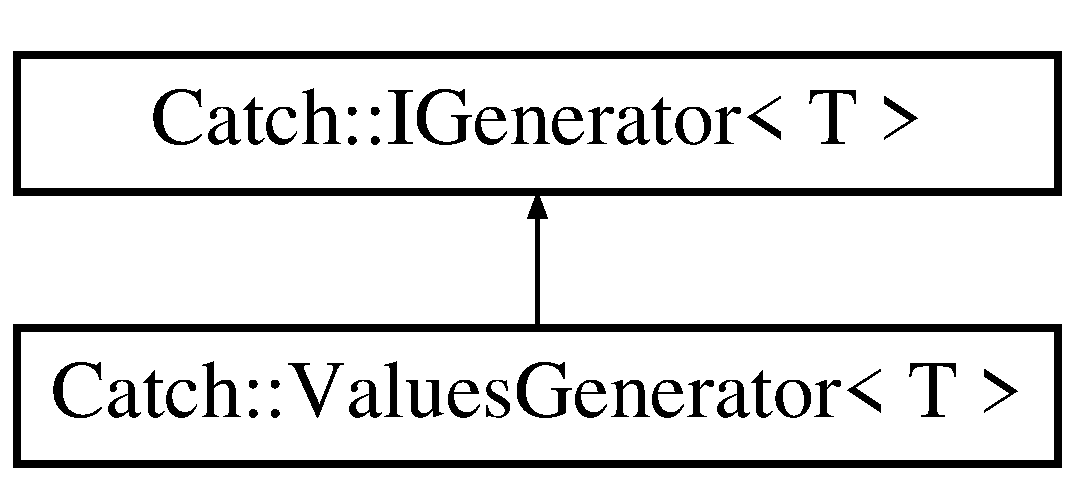
\includegraphics[height=2.000000cm]{class_catch_1_1_values_generator}
\end{center}
\end{figure}
\subsection*{Public Member Functions}
\begin{DoxyCompactItemize}
\item 
\mbox{\hyperlink{class_catch_1_1_values_generator_a36cd3d75afb1f5502400c3ad7cae7a5e}{Values\+Generator}} ()
\item 
void \mbox{\hyperlink{class_catch_1_1_values_generator_a8412c8ce5d9d4fc6ff06d5246d56d538}{add}} (T value)
\item 
virtual T \mbox{\hyperlink{class_catch_1_1_values_generator_a9674c8b70d562d2d68154de92dd1810a}{get\+Value}} (std\+::size\+\_\+t index) const
\item 
virtual std\+::size\+\_\+t \mbox{\hyperlink{class_catch_1_1_values_generator_a9aa5b140ee502975cf35115e534ab771}{size}} () const
\end{DoxyCompactItemize}


\subsection{Constructor \& Destructor Documentation}
\mbox{\Hypertarget{class_catch_1_1_values_generator_a36cd3d75afb1f5502400c3ad7cae7a5e}\label{class_catch_1_1_values_generator_a36cd3d75afb1f5502400c3ad7cae7a5e}} 
\index{Catch\+::\+Values\+Generator@{Catch\+::\+Values\+Generator}!Values\+Generator@{Values\+Generator}}
\index{Values\+Generator@{Values\+Generator}!Catch\+::\+Values\+Generator@{Catch\+::\+Values\+Generator}}
\subsubsection{\texorpdfstring{Values\+Generator()}{ValuesGenerator()}}
{\footnotesize\ttfamily template$<$typename T$>$ \\
\mbox{\hyperlink{class_catch_1_1_values_generator}{Catch\+::\+Values\+Generator}}$<$ T $>$\+::\mbox{\hyperlink{class_catch_1_1_values_generator}{Values\+Generator}} (\begin{DoxyParamCaption}{ }\end{DoxyParamCaption})\hspace{0.3cm}{\ttfamily [inline]}}



\subsection{Member Function Documentation}
\mbox{\Hypertarget{class_catch_1_1_values_generator_a8412c8ce5d9d4fc6ff06d5246d56d538}\label{class_catch_1_1_values_generator_a8412c8ce5d9d4fc6ff06d5246d56d538}} 
\index{Catch\+::\+Values\+Generator@{Catch\+::\+Values\+Generator}!add@{add}}
\index{add@{add}!Catch\+::\+Values\+Generator@{Catch\+::\+Values\+Generator}}
\subsubsection{\texorpdfstring{add()}{add()}}
{\footnotesize\ttfamily template$<$typename T$>$ \\
void \mbox{\hyperlink{class_catch_1_1_values_generator}{Catch\+::\+Values\+Generator}}$<$ T $>$\+::add (\begin{DoxyParamCaption}\item[{T}]{value }\end{DoxyParamCaption})\hspace{0.3cm}{\ttfamily [inline]}}

\mbox{\Hypertarget{class_catch_1_1_values_generator_a9674c8b70d562d2d68154de92dd1810a}\label{class_catch_1_1_values_generator_a9674c8b70d562d2d68154de92dd1810a}} 
\index{Catch\+::\+Values\+Generator@{Catch\+::\+Values\+Generator}!get\+Value@{get\+Value}}
\index{get\+Value@{get\+Value}!Catch\+::\+Values\+Generator@{Catch\+::\+Values\+Generator}}
\subsubsection{\texorpdfstring{get\+Value()}{getValue()}}
{\footnotesize\ttfamily template$<$typename T$>$ \\
virtual T \mbox{\hyperlink{class_catch_1_1_values_generator}{Catch\+::\+Values\+Generator}}$<$ T $>$\+::get\+Value (\begin{DoxyParamCaption}\item[{std\+::size\+\_\+t}]{index }\end{DoxyParamCaption}) const\hspace{0.3cm}{\ttfamily [inline]}, {\ttfamily [virtual]}}



Implements \mbox{\hyperlink{struct_catch_1_1_i_generator_ad69e937cb66dba3ed9429c42abf4fce3}{Catch\+::\+I\+Generator$<$ T $>$}}.

\mbox{\Hypertarget{class_catch_1_1_values_generator_a9aa5b140ee502975cf35115e534ab771}\label{class_catch_1_1_values_generator_a9aa5b140ee502975cf35115e534ab771}} 
\index{Catch\+::\+Values\+Generator@{Catch\+::\+Values\+Generator}!size@{size}}
\index{size@{size}!Catch\+::\+Values\+Generator@{Catch\+::\+Values\+Generator}}
\subsubsection{\texorpdfstring{size()}{size()}}
{\footnotesize\ttfamily template$<$typename T$>$ \\
virtual std\+::size\+\_\+t \mbox{\hyperlink{class_catch_1_1_values_generator}{Catch\+::\+Values\+Generator}}$<$ T $>$\+::size (\begin{DoxyParamCaption}{ }\end{DoxyParamCaption}) const\hspace{0.3cm}{\ttfamily [inline]}, {\ttfamily [virtual]}}



Implements \mbox{\hyperlink{struct_catch_1_1_i_generator_a2e317253b03e838b6065ce69719a198e}{Catch\+::\+I\+Generator$<$ T $>$}}.



The documentation for this class was generated from the following file\+:\begin{DoxyCompactItemize}
\item 
include/\mbox{\hyperlink{catch_8hpp}{catch.\+hpp}}\end{DoxyCompactItemize}

\chapter{File Documentation}
\hypertarget{catch_8hpp}{}\section{include/catch.hpp File Reference}
\label{catch_8hpp}\index{include/catch.\+hpp@{include/catch.\+hpp}}
{\ttfamily \#include $<$sstream$>$}\newline
{\ttfamily \#include $<$algorithm$>$}\newline
{\ttfamily \#include $<$string$>$}\newline
{\ttfamily \#include $<$vector$>$}\newline
{\ttfamily \#include $<$cstddef$>$}\newline
{\ttfamily \#include $<$iomanip$>$}\newline
{\ttfamily \#include $<$limits$>$}\newline
{\ttfamily \#include $<$stdint.\+h$>$}\newline
{\ttfamily \#include $<$stdlib.\+h$>$}\newline
{\ttfamily \#include $<$cmath$>$}\newline
{\ttfamily \#include $<$set$>$}\newline
\subsection*{Classes}
\begin{DoxyCompactItemize}
\item 
struct \mbox{\hyperlink{struct_catch_1_1_case_sensitive}{Catch\+::\+Case\+Sensitive}}
\item 
class \mbox{\hyperlink{class_catch_1_1_non_copyable}{Catch\+::\+Non\+Copyable}}
\item 
class \mbox{\hyperlink{class_catch_1_1_safe_bool}{Catch\+::\+Safe\+Bool}}
\item 
struct \mbox{\hyperlink{struct_catch_1_1pluralise}{Catch\+::pluralise}}
\item 
struct \mbox{\hyperlink{struct_catch_1_1_source_line_info}{Catch\+::\+Source\+Line\+Info}}
\item 
struct \mbox{\hyperlink{struct_catch_1_1_stream_end_stop}{Catch\+::\+Stream\+End\+Stop}}
\item 
class \mbox{\hyperlink{class_catch_1_1_not_implemented_exception}{Catch\+::\+Not\+Implemented\+Exception}}
\item 
struct \mbox{\hyperlink{struct_catch_1_1_i_generator_info}{Catch\+::\+I\+Generator\+Info}}
\item 
struct \mbox{\hyperlink{struct_catch_1_1_i_generators_for_test}{Catch\+::\+I\+Generators\+For\+Test}}
\item 
class \mbox{\hyperlink{class_catch_1_1_ptr}{Catch\+::\+Ptr$<$ T $>$}}
\item 
struct \mbox{\hyperlink{struct_catch_1_1_i_shared}{Catch\+::\+I\+Shared}}
\item 
struct \mbox{\hyperlink{struct_catch_1_1_shared_impl}{Catch\+::\+Shared\+Impl$<$ T $>$}}
\item 
struct \mbox{\hyperlink{struct_catch_1_1_i_context}{Catch\+::\+I\+Context}}
\item 
struct \mbox{\hyperlink{struct_catch_1_1_i_mutable_context}{Catch\+::\+I\+Mutable\+Context}}
\item 
struct \mbox{\hyperlink{struct_catch_1_1_i_test_case}{Catch\+::\+I\+Test\+Case}}
\item 
struct \mbox{\hyperlink{struct_catch_1_1_i_test_case_registry}{Catch\+::\+I\+Test\+Case\+Registry}}
\item 
class \mbox{\hyperlink{class_catch_1_1_method_test_case}{Catch\+::\+Method\+Test\+Case$<$ C $>$}}
\item 
struct \mbox{\hyperlink{struct_catch_1_1_name_and_desc}{Catch\+::\+Name\+And\+Desc}}
\item 
struct \mbox{\hyperlink{struct_catch_1_1_auto_reg}{Catch\+::\+Auto\+Reg}}
\item 
struct \mbox{\hyperlink{struct_catch_1_1_result_was}{Catch\+::\+Result\+Was}}
\item 
struct \mbox{\hyperlink{struct_catch_1_1_result_disposition}{Catch\+::\+Result\+Disposition}}
\item 
struct \mbox{\hyperlink{struct_catch_1_1_decomposed_expression}{Catch\+::\+Decomposed\+Expression}}
\item 
struct \mbox{\hyperlink{struct_catch_1_1_assertion_info}{Catch\+::\+Assertion\+Info}}
\item 
struct \mbox{\hyperlink{struct_catch_1_1_assertion_result_data}{Catch\+::\+Assertion\+Result\+Data}}
\item 
class \mbox{\hyperlink{class_catch_1_1_assertion_result}{Catch\+::\+Assertion\+Result}}
\item 
struct \mbox{\hyperlink{struct_catch_1_1_matchers_1_1_impl_1_1_match_all_of}{Catch\+::\+Matchers\+::\+Impl\+::\+Match\+All\+Of$<$ Arg\+T $>$}}
\item 
struct \mbox{\hyperlink{struct_catch_1_1_matchers_1_1_impl_1_1_match_any_of}{Catch\+::\+Matchers\+::\+Impl\+::\+Match\+Any\+Of$<$ Arg\+T $>$}}
\item 
struct \mbox{\hyperlink{struct_catch_1_1_matchers_1_1_impl_1_1_match_not_of}{Catch\+::\+Matchers\+::\+Impl\+::\+Match\+Not\+Of$<$ Arg\+T $>$}}
\item 
class \mbox{\hyperlink{class_catch_1_1_matchers_1_1_impl_1_1_matcher_untyped_base}{Catch\+::\+Matchers\+::\+Impl\+::\+Matcher\+Untyped\+Base}}
\item 
struct \mbox{\hyperlink{struct_catch_1_1_matchers_1_1_impl_1_1_matcher_method}{Catch\+::\+Matchers\+::\+Impl\+::\+Matcher\+Method$<$ Object\+T $>$}}
\item 
struct \mbox{\hyperlink{struct_catch_1_1_matchers_1_1_impl_1_1_matcher_method_3_01_ptr_t_01_5_01_4}{Catch\+::\+Matchers\+::\+Impl\+::\+Matcher\+Method$<$ Ptr\+T $\ast$ $>$}}
\item 
struct \mbox{\hyperlink{struct_catch_1_1_matchers_1_1_impl_1_1_matcher_base}{Catch\+::\+Matchers\+::\+Impl\+::\+Matcher\+Base$<$ Object\+T, Comparator\+T $>$}}
\item 
struct \mbox{\hyperlink{struct_catch_1_1_matchers_1_1_impl_1_1_match_all_of}{Catch\+::\+Matchers\+::\+Impl\+::\+Match\+All\+Of$<$ Arg\+T $>$}}
\item 
struct \mbox{\hyperlink{struct_catch_1_1_matchers_1_1_impl_1_1_match_any_of}{Catch\+::\+Matchers\+::\+Impl\+::\+Match\+Any\+Of$<$ Arg\+T $>$}}
\item 
struct \mbox{\hyperlink{struct_catch_1_1_matchers_1_1_impl_1_1_match_not_of}{Catch\+::\+Matchers\+::\+Impl\+::\+Match\+Not\+Of$<$ Arg\+T $>$}}
\item 
struct \mbox{\hyperlink{struct_catch_1_1_test_failure_exception}{Catch\+::\+Test\+Failure\+Exception}}
\item 
class \mbox{\hyperlink{class_catch_1_1_expression_lhs}{Catch\+::\+Expression\+Lhs$<$ T $>$}}
\item 
struct \mbox{\hyperlink{struct_catch_1_1_copyable_stream}{Catch\+::\+Copyable\+Stream}}
\item 
class \mbox{\hyperlink{class_catch_1_1_result_builder}{Catch\+::\+Result\+Builder}}
\item 
struct \mbox{\hyperlink{struct_catch_1_1_internal_1_1_operator_traits}{Catch\+::\+Internal\+::\+Operator\+Traits$<$ Op $>$}}
\item 
struct \mbox{\hyperlink{struct_catch_1_1_internal_1_1_operator_traits_3_01_is_equal_to_01_4}{Catch\+::\+Internal\+::\+Operator\+Traits$<$ Is\+Equal\+To $>$}}
\item 
struct \mbox{\hyperlink{struct_catch_1_1_internal_1_1_operator_traits_3_01_is_not_equal_to_01_4}{Catch\+::\+Internal\+::\+Operator\+Traits$<$ Is\+Not\+Equal\+To $>$}}
\item 
struct \mbox{\hyperlink{struct_catch_1_1_internal_1_1_operator_traits_3_01_is_less_than_01_4}{Catch\+::\+Internal\+::\+Operator\+Traits$<$ Is\+Less\+Than $>$}}
\item 
struct \mbox{\hyperlink{struct_catch_1_1_internal_1_1_operator_traits_3_01_is_greater_than_01_4}{Catch\+::\+Internal\+::\+Operator\+Traits$<$ Is\+Greater\+Than $>$}}
\item 
struct \mbox{\hyperlink{struct_catch_1_1_internal_1_1_operator_traits_3_01_is_less_than_or_equal_to_01_4}{Catch\+::\+Internal\+::\+Operator\+Traits$<$ Is\+Less\+Than\+Or\+Equal\+To $>$}}
\item 
struct \mbox{\hyperlink{struct_catch_1_1_internal_1_1_operator_traits_3_01_is_greater_than_or_equal_to_01_4}{Catch\+::\+Internal\+::\+Operator\+Traits$<$ Is\+Greater\+Than\+Or\+Equal\+To $>$}}
\item 
class \mbox{\hyperlink{class_catch_1_1_internal_1_1_evaluator}{Catch\+::\+Internal\+::\+Evaluator$<$ T1, T2, Op $>$}}
\item 
struct \mbox{\hyperlink{struct_catch_1_1_internal_1_1_evaluator_3_01_t1_00_01_t2_00_01_is_equal_to_01_4}{Catch\+::\+Internal\+::\+Evaluator$<$ T1, T2, Is\+Equal\+To $>$}}
\item 
struct \mbox{\hyperlink{struct_catch_1_1_internal_1_1_evaluator_3_01_t1_00_01_t2_00_01_is_not_equal_to_01_4}{Catch\+::\+Internal\+::\+Evaluator$<$ T1, T2, Is\+Not\+Equal\+To $>$}}
\item 
struct \mbox{\hyperlink{struct_catch_1_1_internal_1_1_evaluator_3_01_t1_00_01_t2_00_01_is_less_than_01_4}{Catch\+::\+Internal\+::\+Evaluator$<$ T1, T2, Is\+Less\+Than $>$}}
\item 
struct \mbox{\hyperlink{struct_catch_1_1_internal_1_1_evaluator_3_01_t1_00_01_t2_00_01_is_greater_than_01_4}{Catch\+::\+Internal\+::\+Evaluator$<$ T1, T2, Is\+Greater\+Than $>$}}
\item 
struct \mbox{\hyperlink{struct_catch_1_1_internal_1_1_evaluator_3_01_t1_00_01_t2_00_01_is_greater_than_or_equal_to_01_4}{Catch\+::\+Internal\+::\+Evaluator$<$ T1, T2, Is\+Greater\+Than\+Or\+Equal\+To $>$}}
\item 
struct \mbox{\hyperlink{struct_catch_1_1_internal_1_1_evaluator_3_01_t1_00_01_t2_00_01_is_less_than_or_equal_to_01_4}{Catch\+::\+Internal\+::\+Evaluator$<$ T1, T2, Is\+Less\+Than\+Or\+Equal\+To $>$}}
\item 
struct \mbox{\hyperlink{struct_catch_1_1_detail_1_1_borg_type}{Catch\+::\+Detail\+::\+Borg\+Type}}
\item 
struct \mbox{\hyperlink{struct_catch_1_1_detail_1_1_true_type}{Catch\+::\+Detail\+::\+True\+Type}}
\item 
struct \mbox{\hyperlink{struct_catch_1_1_detail_1_1_false_type}{Catch\+::\+Detail\+::\+False\+Type}}
\item 
struct \mbox{\hyperlink{struct_catch_1_1_detail_1_1_is_stream_insertable}{Catch\+::\+Detail\+::\+Is\+Stream\+Insertable$<$ T $>$}}
\item 
struct \mbox{\hyperlink{struct_catch_1_1_detail_1_1_string_maker_base}{Catch\+::\+Detail\+::\+String\+Maker\+Base$<$ C $>$}}
\item 
struct \mbox{\hyperlink{struct_catch_1_1_detail_1_1_string_maker_base_3_01true_01_4}{Catch\+::\+Detail\+::\+String\+Maker\+Base$<$ true $>$}}
\item 
struct \mbox{\hyperlink{struct_catch_1_1_string_maker}{Catch\+::\+String\+Maker$<$ T $>$}}
\item 
struct \mbox{\hyperlink{struct_catch_1_1_string_maker_3_01_t_01_5_01_4}{Catch\+::\+String\+Maker$<$ T $\ast$ $>$}}
\item 
struct \mbox{\hyperlink{struct_catch_1_1_string_maker_3_01_r_01_c_1_1_5_01_4}{Catch\+::\+String\+Maker$<$ R C\+::$\ast$ $>$}}
\item 
class \mbox{\hyperlink{class_catch_1_1_binary_expression}{Catch\+::\+Binary\+Expression$<$ Lhs\+T, Op, Rhs\+T $>$}}
\item 
class \mbox{\hyperlink{class_catch_1_1_match_expression}{Catch\+::\+Match\+Expression$<$ Arg\+T, Matcher\+T $>$}}
\item 
class \mbox{\hyperlink{class_catch_1_1_expression_lhs}{Catch\+::\+Expression\+Lhs$<$ T $>$}}
\item 
class \mbox{\hyperlink{class_catch_1_1_binary_expression}{Catch\+::\+Binary\+Expression$<$ Lhs\+T, Op, Rhs\+T $>$}}
\item 
class \mbox{\hyperlink{class_catch_1_1_match_expression}{Catch\+::\+Match\+Expression$<$ Arg\+T, Matcher\+T $>$}}
\item 
struct \mbox{\hyperlink{struct_catch_1_1_message_info}{Catch\+::\+Message\+Info}}
\item 
struct \mbox{\hyperlink{struct_catch_1_1_message_builder}{Catch\+::\+Message\+Builder}}
\item 
class \mbox{\hyperlink{class_catch_1_1_scoped_message}{Catch\+::\+Scoped\+Message}}
\item 
struct \mbox{\hyperlink{struct_catch_1_1_i_result_capture}{Catch\+::\+I\+Result\+Capture}}
\item 
struct \mbox{\hyperlink{struct_catch_1_1_i_runner}{Catch\+::\+I\+Runner}}
\item 
struct \mbox{\hyperlink{struct_catch_1_1_counts}{Catch\+::\+Counts}}
\item 
struct \mbox{\hyperlink{struct_catch_1_1_totals}{Catch\+::\+Totals}}
\item 
struct \mbox{\hyperlink{struct_catch_1_1_section_info}{Catch\+::\+Section\+Info}}
\item 
struct \mbox{\hyperlink{struct_catch_1_1_section_end_info}{Catch\+::\+Section\+End\+Info}}
\item 
class \mbox{\hyperlink{class_catch_1_1_timer}{Catch\+::\+Timer}}
\item 
class \mbox{\hyperlink{class_catch_1_1_section}{Catch\+::\+Section}}
\item 
struct \mbox{\hyperlink{struct_catch_1_1_i_generator}{Catch\+::\+I\+Generator$<$ T $>$}}
\item 
class \mbox{\hyperlink{class_catch_1_1_between_generator}{Catch\+::\+Between\+Generator$<$ T $>$}}
\item 
class \mbox{\hyperlink{class_catch_1_1_values_generator}{Catch\+::\+Values\+Generator$<$ T $>$}}
\item 
class \mbox{\hyperlink{class_catch_1_1_composite_generator}{Catch\+::\+Composite\+Generator$<$ T $>$}}
\item 
struct \mbox{\hyperlink{struct_catch_1_1_i_registry_hub}{Catch\+::\+I\+Registry\+Hub}}
\item 
struct \mbox{\hyperlink{struct_catch_1_1_i_mutable_registry_hub}{Catch\+::\+I\+Mutable\+Registry\+Hub}}
\item 
struct \mbox{\hyperlink{struct_catch_1_1_i_exception_translator}{Catch\+::\+I\+Exception\+Translator}}
\item 
struct \mbox{\hyperlink{struct_catch_1_1_i_exception_translator_registry}{Catch\+::\+I\+Exception\+Translator\+Registry}}
\item 
class \mbox{\hyperlink{class_catch_1_1_exception_translator_registrar}{Catch\+::\+Exception\+Translator\+Registrar}}
\item 
class \mbox{\hyperlink{class_catch_1_1_detail_1_1_approx}{Catch\+::\+Detail\+::\+Approx}}
\item 
struct \mbox{\hyperlink{struct_catch_1_1_matchers_1_1_std_string_1_1_cased_string}{Catch\+::\+Matchers\+::\+Std\+String\+::\+Cased\+String}}
\item 
struct \mbox{\hyperlink{struct_catch_1_1_matchers_1_1_std_string_1_1_string_matcher_base}{Catch\+::\+Matchers\+::\+Std\+String\+::\+String\+Matcher\+Base}}
\item 
struct \mbox{\hyperlink{struct_catch_1_1_matchers_1_1_std_string_1_1_equals_matcher}{Catch\+::\+Matchers\+::\+Std\+String\+::\+Equals\+Matcher}}
\item 
struct \mbox{\hyperlink{struct_catch_1_1_matchers_1_1_std_string_1_1_contains_matcher}{Catch\+::\+Matchers\+::\+Std\+String\+::\+Contains\+Matcher}}
\item 
struct \mbox{\hyperlink{struct_catch_1_1_matchers_1_1_std_string_1_1_starts_with_matcher}{Catch\+::\+Matchers\+::\+Std\+String\+::\+Starts\+With\+Matcher}}
\item 
struct \mbox{\hyperlink{struct_catch_1_1_matchers_1_1_std_string_1_1_ends_with_matcher}{Catch\+::\+Matchers\+::\+Std\+String\+::\+Ends\+With\+Matcher}}
\item 
struct \mbox{\hyperlink{struct_catch_1_1_matchers_1_1_vector_1_1_contains_element_matcher}{Catch\+::\+Matchers\+::\+Vector\+::\+Contains\+Element\+Matcher$<$ T $>$}}
\item 
struct \mbox{\hyperlink{struct_catch_1_1_matchers_1_1_vector_1_1_contains_matcher}{Catch\+::\+Matchers\+::\+Vector\+::\+Contains\+Matcher$<$ T $>$}}
\item 
struct \mbox{\hyperlink{struct_catch_1_1_matchers_1_1_vector_1_1_equals_matcher}{Catch\+::\+Matchers\+::\+Vector\+::\+Equals\+Matcher$<$ T $>$}}
\item 
struct \mbox{\hyperlink{struct_catch_1_1_tag_alias}{Catch\+::\+Tag\+Alias}}
\item 
struct \mbox{\hyperlink{struct_catch_1_1_registrar_for_tag_aliases}{Catch\+::\+Registrar\+For\+Tag\+Aliases}}
\item 
class \mbox{\hyperlink{class_catch_1_1_option}{Catch\+::\+Option$<$ T $>$}}
\item 
struct \mbox{\hyperlink{struct_catch_1_1_i_tag_alias_registry}{Catch\+::\+I\+Tag\+Alias\+Registry}}
\item 
struct \mbox{\hyperlink{struct_catch_1_1_test_case_info}{Catch\+::\+Test\+Case\+Info}}
\item 
class \mbox{\hyperlink{class_catch_1_1_test_case}{Catch\+::\+Test\+Case}}
\end{DoxyCompactItemize}
\subsection*{Namespaces}
\begin{DoxyCompactItemize}
\item 
 \mbox{\hyperlink{namespace_catch}{Catch}}
\item 
 \mbox{\hyperlink{namespace_catch_1_1_matchers}{Catch\+::\+Matchers}}
\item 
 \mbox{\hyperlink{namespace_catch_1_1_matchers_1_1_impl}{Catch\+::\+Matchers\+::\+Impl}}
\item 
 \mbox{\hyperlink{namespace_catch_1_1_internal}{Catch\+::\+Internal}}
\item 
 \mbox{\hyperlink{namespace_catch_1_1_detail}{Catch\+::\+Detail}}
\item 
 \mbox{\hyperlink{namespace_catch_1_1_generators}{Catch\+::\+Generators}}
\item 
 \mbox{\hyperlink{namespace_catch_1_1_matchers_1_1_std_string}{Catch\+::\+Matchers\+::\+Std\+String}}
\item 
 \mbox{\hyperlink{namespace_catch_1_1_matchers_1_1_vector}{Catch\+::\+Matchers\+::\+Vector}}
\end{DoxyCompactItemize}
\subsection*{Macros}
\begin{DoxyCompactItemize}
\item 
\#define \mbox{\hyperlink{catch_8hpp_a24243dc93e4f452db07fb6514bb9e749}{T\+W\+O\+B\+L\+U\+E\+C\+U\+B\+E\+S\+\_\+\+C\+A\+T\+C\+H\+\_\+\+H\+P\+P\+\_\+\+I\+N\+C\+L\+U\+D\+ED}}
\item 
\#define \mbox{\hyperlink{catch_8hpp_a62f025f954221470c23a77e90ffacd56}{T\+W\+O\+B\+L\+U\+E\+C\+U\+B\+E\+S\+\_\+\+C\+A\+T\+C\+H\+\_\+\+N\+O\+T\+I\+M\+P\+L\+E\+M\+E\+N\+T\+E\+D\+\_\+\+E\+X\+C\+E\+P\+T\+I\+O\+N\+\_\+\+H\+\_\+\+I\+N\+C\+L\+U\+D\+ED}}
\item 
\#define \mbox{\hyperlink{catch_8hpp_a27b42830f93b62d65bd7c15fb3acd0d0}{T\+W\+O\+B\+L\+U\+E\+C\+U\+B\+E\+S\+\_\+\+C\+A\+T\+C\+H\+\_\+\+C\+O\+M\+M\+O\+N\+\_\+\+H\+\_\+\+I\+N\+C\+L\+U\+D\+ED}}
\item 
\#define \mbox{\hyperlink{catch_8hpp_ae20e90c8b19224675d022f94b534ef6b}{T\+W\+O\+B\+L\+U\+E\+C\+U\+B\+E\+S\+\_\+\+C\+A\+T\+C\+H\+\_\+\+C\+O\+M\+P\+I\+L\+E\+R\+\_\+\+C\+A\+P\+A\+B\+I\+L\+I\+T\+I\+E\+S\+\_\+\+H\+P\+P\+\_\+\+I\+N\+C\+L\+U\+D\+ED}}
\item 
\#define \mbox{\hyperlink{catch_8hpp_ac5eee4f90512985d2043f971c6f08707}{C\+A\+T\+C\+H\+\_\+\+C\+O\+N\+F\+I\+G\+\_\+\+P\+O\+S\+I\+X\+\_\+\+S\+I\+G\+N\+A\+LS}}
\item 
\#define \mbox{\hyperlink{catch_8hpp_a89c1608a68775aca1bb7c265f7ba923a}{C\+A\+T\+C\+H\+\_\+\+I\+N\+T\+E\+R\+N\+A\+L\+\_\+\+S\+U\+P\+P\+R\+E\+S\+S\+\_\+\+P\+A\+R\+E\+N\+T\+H\+E\+S\+E\+S\+\_\+\+W\+A\+R\+N\+I\+N\+GS}}
\item 
\#define \mbox{\hyperlink{catch_8hpp_aec1f55c22f26366aaad1467206352792}{C\+A\+T\+C\+H\+\_\+\+I\+N\+T\+E\+R\+N\+A\+L\+\_\+\+U\+N\+S\+U\+P\+P\+R\+E\+S\+S\+\_\+\+P\+A\+R\+E\+N\+T\+H\+E\+S\+E\+S\+\_\+\+W\+A\+R\+N\+I\+N\+GS}}
\item 
\#define \mbox{\hyperlink{catch_8hpp_a4b2e2bb73fa06786f087c10d070e8411}{C\+A\+T\+C\+H\+\_\+\+I\+N\+T\+E\+R\+N\+A\+L\+\_\+\+S\+U\+P\+P\+R\+E\+S\+S\+\_\+\+E\+T\+D\+\_\+\+W\+A\+R\+N\+I\+N\+GS}}
\item 
\#define \mbox{\hyperlink{catch_8hpp_af29a2e0d5c057486545c35f955546291}{C\+A\+T\+C\+H\+\_\+\+I\+N\+T\+E\+R\+N\+A\+L\+\_\+\+U\+N\+S\+U\+P\+P\+R\+E\+S\+S\+\_\+\+E\+T\+D\+\_\+\+W\+A\+R\+N\+I\+N\+GS}}
\item 
\#define \mbox{\hyperlink{catch_8hpp_a0408e94ca73880d41f38852b68eadb3c}{C\+A\+T\+C\+H\+\_\+\+N\+O\+E\+X\+C\+E\+PT}}~throw()
\item 
\#define \mbox{\hyperlink{catch_8hpp_a61ef049189c00120bf4d1641477e509c}{C\+A\+T\+C\+H\+\_\+\+N\+O\+E\+X\+C\+E\+P\+T\+\_\+\+IS}}(x)
\item 
\#define \mbox{\hyperlink{catch_8hpp_a408e2cfae3f9ae3790da2d647a859a88}{C\+A\+T\+C\+H\+\_\+\+N\+U\+LL}}~N\+U\+LL
\item 
\#define \mbox{\hyperlink{catch_8hpp_a8ecdce4d3f57835f707915ae831eb847}{C\+A\+T\+C\+H\+\_\+\+O\+V\+E\+R\+R\+I\+DE}}
\item 
\#define \mbox{\hyperlink{catch_8hpp_afebdae626caac99de5b11b63fbd41d90}{C\+A\+T\+C\+H\+\_\+\+A\+U\+T\+O\+\_\+\+P\+TR}}(T)~std\+::auto\+\_\+ptr$<$T$>$
\item 
\#define \mbox{\hyperlink{catch_8hpp_a7c21e89d8b7727757ce9ca2b848f1cda}{I\+N\+T\+E\+R\+N\+A\+L\+\_\+\+C\+A\+T\+C\+H\+\_\+\+U\+N\+I\+Q\+U\+E\+\_\+\+N\+A\+M\+E\+\_\+\+L\+I\+N\+E2}}(name,  line)~name\#\#line
\item 
\#define \mbox{\hyperlink{catch_8hpp_a1b51a086ea21a750bd306ac0ed4d2a95}{I\+N\+T\+E\+R\+N\+A\+L\+\_\+\+C\+A\+T\+C\+H\+\_\+\+U\+N\+I\+Q\+U\+E\+\_\+\+N\+A\+M\+E\+\_\+\+L\+I\+NE}}(name,  line)~\mbox{\hyperlink{catch_8hpp_a7c21e89d8b7727757ce9ca2b848f1cda}{I\+N\+T\+E\+R\+N\+A\+L\+\_\+\+C\+A\+T\+C\+H\+\_\+\+U\+N\+I\+Q\+U\+E\+\_\+\+N\+A\+M\+E\+\_\+\+L\+I\+N\+E2}}( name, line )
\item 
\#define \mbox{\hyperlink{catch_8hpp_afe320ceec108fc8c160f9ac3938f1bc8}{I\+N\+T\+E\+R\+N\+A\+L\+\_\+\+C\+A\+T\+C\+H\+\_\+\+U\+N\+I\+Q\+U\+E\+\_\+\+N\+A\+ME}}(name)~\mbox{\hyperlink{catch_8hpp_a1b51a086ea21a750bd306ac0ed4d2a95}{I\+N\+T\+E\+R\+N\+A\+L\+\_\+\+C\+A\+T\+C\+H\+\_\+\+U\+N\+I\+Q\+U\+E\+\_\+\+N\+A\+M\+E\+\_\+\+L\+I\+NE}}( name, \+\_\+\+\_\+\+L\+I\+N\+E\+\_\+\+\_\+ )
\item 
\#define \mbox{\hyperlink{catch_8hpp_af5d658c0f6223019fd91fda2dc8bff78}{I\+N\+T\+E\+R\+N\+A\+L\+\_\+\+C\+A\+T\+C\+H\+\_\+\+S\+T\+R\+I\+N\+G\+I\+F\+Y2}}(expr)~\#expr
\item 
\#define \mbox{\hyperlink{catch_8hpp_ae5403b344db1b68faf372ad1dbcb5791}{I\+N\+T\+E\+R\+N\+A\+L\+\_\+\+C\+A\+T\+C\+H\+\_\+\+S\+T\+R\+I\+N\+G\+I\+FY}}(expr)~\mbox{\hyperlink{catch_8hpp_af5d658c0f6223019fd91fda2dc8bff78}{I\+N\+T\+E\+R\+N\+A\+L\+\_\+\+C\+A\+T\+C\+H\+\_\+\+S\+T\+R\+I\+N\+G\+I\+F\+Y2}}( expr )
\item 
\#define \mbox{\hyperlink{catch_8hpp_abc0b2405454c51748a31e0393d9ad5d1}{C\+A\+T\+C\+H\+\_\+\+I\+N\+T\+E\+R\+N\+A\+L\+\_\+\+L\+I\+N\+E\+I\+N\+FO}}~\+::\mbox{\hyperlink{struct_catch_1_1_source_line_info}{Catch\+::\+Source\+Line\+Info}}( \+\_\+\+\_\+\+F\+I\+L\+E\+\_\+\+\_\+, static\+\_\+cast$<$std\+::size\+\_\+t$>$( \+\_\+\+\_\+\+L\+I\+N\+E\+\_\+\+\_\+ ) )
\item 
\#define \mbox{\hyperlink{catch_8hpp_a05b6c8a530fa2e5b397add8966522777}{C\+A\+T\+C\+H\+\_\+\+I\+N\+T\+E\+R\+N\+A\+L\+\_\+\+E\+R\+R\+OR}}(msg)~\+::\mbox{\hyperlink{namespace_catch_a702b612f683d154c466ea8297ed4a20d}{Catch\+::throw\+Logic\+Error}}( msg, \mbox{\hyperlink{catch_8hpp_abc0b2405454c51748a31e0393d9ad5d1}{C\+A\+T\+C\+H\+\_\+\+I\+N\+T\+E\+R\+N\+A\+L\+\_\+\+L\+I\+N\+E\+I\+N\+FO}} );
\item 
\#define \mbox{\hyperlink{catch_8hpp_ae717ef7d955c82073b1aae5a1d2de0ae}{C\+A\+T\+C\+H\+\_\+\+N\+O\+T\+\_\+\+I\+M\+P\+L\+E\+M\+E\+N\+T\+ED}}~throw \mbox{\hyperlink{class_catch_1_1_not_implemented_exception}{Catch\+::\+Not\+Implemented\+Exception}}( \mbox{\hyperlink{catch_8hpp_abc0b2405454c51748a31e0393d9ad5d1}{C\+A\+T\+C\+H\+\_\+\+I\+N\+T\+E\+R\+N\+A\+L\+\_\+\+L\+I\+N\+E\+I\+N\+FO}} )
\item 
\#define \mbox{\hyperlink{catch_8hpp_a07a1c68dee179942c1aede4f9b304543}{T\+W\+O\+B\+L\+U\+E\+C\+U\+B\+E\+S\+\_\+\+C\+A\+T\+C\+H\+\_\+\+C\+O\+N\+T\+E\+X\+T\+\_\+\+H\+\_\+\+I\+N\+C\+L\+U\+D\+ED}}
\item 
\#define \mbox{\hyperlink{catch_8hpp_a70327cb83c2141b3b54e9549418021ad}{T\+W\+O\+B\+L\+U\+E\+C\+U\+B\+E\+S\+\_\+\+C\+A\+T\+C\+H\+\_\+\+I\+N\+T\+E\+R\+F\+A\+C\+E\+S\+\_\+\+G\+E\+N\+E\+R\+A\+T\+O\+R\+S\+\_\+\+H\+\_\+\+I\+N\+C\+L\+U\+D\+ED}}
\item 
\#define \mbox{\hyperlink{catch_8hpp_af6024c3338ada36de16549522ec8f4dd}{T\+W\+O\+B\+L\+U\+E\+C\+U\+B\+E\+S\+\_\+\+C\+A\+T\+C\+H\+\_\+\+P\+T\+R\+\_\+\+H\+P\+P\+\_\+\+I\+N\+C\+L\+U\+D\+ED}}
\item 
\#define \mbox{\hyperlink{catch_8hpp_a202df3911846a6f2281d940b29b84824}{T\+W\+O\+B\+L\+U\+E\+C\+U\+B\+E\+S\+\_\+\+C\+A\+T\+C\+H\+\_\+\+T\+E\+S\+T\+\_\+\+R\+E\+G\+I\+S\+T\+R\+Y\+\_\+\+H\+P\+P\+\_\+\+I\+N\+C\+L\+U\+D\+ED}}
\item 
\#define \mbox{\hyperlink{catch_8hpp_a57d04225b51dece606932db63aebeb5f}{T\+W\+O\+B\+L\+U\+E\+C\+U\+B\+E\+S\+\_\+\+C\+A\+T\+C\+H\+\_\+\+I\+N\+T\+E\+R\+F\+A\+C\+E\+S\+\_\+\+T\+E\+S\+T\+C\+A\+S\+E\+\_\+\+H\+\_\+\+I\+N\+C\+L\+U\+D\+ED}}
\item 
\#define \mbox{\hyperlink{catch_8hpp_ab4059fa3e4a47e9475c1056e6808d144}{I\+N\+T\+E\+R\+N\+A\+L\+\_\+\+C\+A\+T\+C\+H\+\_\+\+T\+E\+S\+T\+C\+A\+S\+E2}}(Test\+Name,  Name,  Desc)
\item 
\#define \mbox{\hyperlink{catch_8hpp_a1cb98d355207a372c71f19ea989eb0cc}{I\+N\+T\+E\+R\+N\+A\+L\+\_\+\+C\+A\+T\+C\+H\+\_\+\+T\+E\+S\+T\+C\+A\+SE}}(Name,  Desc)~\mbox{\hyperlink{catch_8hpp_ab4059fa3e4a47e9475c1056e6808d144}{I\+N\+T\+E\+R\+N\+A\+L\+\_\+\+C\+A\+T\+C\+H\+\_\+\+T\+E\+S\+T\+C\+A\+S\+E2}}( \mbox{\hyperlink{catch_8hpp_afe320ceec108fc8c160f9ac3938f1bc8}{I\+N\+T\+E\+R\+N\+A\+L\+\_\+\+C\+A\+T\+C\+H\+\_\+\+U\+N\+I\+Q\+U\+E\+\_\+\+N\+A\+ME}}( \+\_\+\+\_\+\+\_\+\+\_\+\+C\+\_\+\+A\+\_\+\+T\+\_\+\+C\+\_\+\+H\+\_\+\+\_\+\+\_\+\+\_\+\+T\+\_\+\+E\+\_\+\+S\+\_\+\+T\+\_\+\+\_\+\+\_\+\+\_\+ ), Name, Desc )
\item 
\#define \mbox{\hyperlink{catch_8hpp_a668f4d27507d64accd74ca9fb5c66176}{I\+N\+T\+E\+R\+N\+A\+L\+\_\+\+C\+A\+T\+C\+H\+\_\+\+M\+E\+T\+H\+O\+D\+\_\+\+A\+S\+\_\+\+T\+E\+S\+T\+\_\+\+C\+A\+SE}}(Qualified\+Method,  Name,  Desc)
\item 
\#define \mbox{\hyperlink{catch_8hpp_a72097450f11ad05c90a0e1a77ef96e05}{I\+N\+T\+E\+R\+N\+A\+L\+\_\+\+C\+A\+T\+C\+H\+\_\+\+T\+E\+S\+T\+\_\+\+C\+A\+S\+E\+\_\+\+M\+E\+T\+H\+O\+D2}}(Test\+Case\+Name,  Class\+Name,  Test\+Name,  Desc)
\item 
\#define \mbox{\hyperlink{catch_8hpp_a46bb9f683226dfa2c857dd62af7aa106}{I\+N\+T\+E\+R\+N\+A\+L\+\_\+\+C\+A\+T\+C\+H\+\_\+\+T\+E\+S\+T\+\_\+\+C\+A\+S\+E\+\_\+\+M\+E\+T\+H\+OD}}(Class\+Name,  Test\+Name,  Desc)~\mbox{\hyperlink{catch_8hpp_a72097450f11ad05c90a0e1a77ef96e05}{I\+N\+T\+E\+R\+N\+A\+L\+\_\+\+C\+A\+T\+C\+H\+\_\+\+T\+E\+S\+T\+\_\+\+C\+A\+S\+E\+\_\+\+M\+E\+T\+H\+O\+D2}}( \mbox{\hyperlink{catch_8hpp_afe320ceec108fc8c160f9ac3938f1bc8}{I\+N\+T\+E\+R\+N\+A\+L\+\_\+\+C\+A\+T\+C\+H\+\_\+\+U\+N\+I\+Q\+U\+E\+\_\+\+N\+A\+ME}}( \+\_\+\+\_\+\+\_\+\+\_\+\+C\+\_\+\+A\+\_\+\+T\+\_\+\+C\+\_\+\+H\+\_\+\+\_\+\+\_\+\+\_\+\+T\+\_\+\+E\+\_\+\+S\+\_\+\+T\+\_\+\+\_\+\+\_\+\+\_\+ ), Class\+Name, Test\+Name, Desc )
\item 
\#define \mbox{\hyperlink{catch_8hpp_a2c89fdef42502a2b2e34b58cea9f68ff}{I\+N\+T\+E\+R\+N\+A\+L\+\_\+\+C\+A\+T\+C\+H\+\_\+\+R\+E\+G\+I\+S\+T\+E\+R\+\_\+\+T\+E\+S\+T\+C\+A\+SE}}(Function,  Name,  Desc)
\item 
\#define \mbox{\hyperlink{catch_8hpp_af06e9a04b0106596b7645d81e1aba5c0}{T\+W\+O\+B\+L\+U\+E\+C\+U\+B\+E\+S\+\_\+\+C\+A\+T\+C\+H\+\_\+\+C\+A\+P\+T\+U\+R\+E\+\_\+\+H\+P\+P\+\_\+\+I\+N\+C\+L\+U\+D\+ED}}
\item 
\#define \mbox{\hyperlink{catch_8hpp_a41060a914a029983a3a9db8d50724329}{T\+W\+O\+B\+L\+U\+E\+C\+U\+B\+E\+S\+\_\+\+C\+A\+T\+C\+H\+\_\+\+R\+E\+S\+U\+L\+T\+\_\+\+B\+U\+I\+L\+D\+E\+R\+\_\+\+H\+\_\+\+I\+N\+C\+L\+U\+D\+ED}}
\item 
\#define \mbox{\hyperlink{catch_8hpp_aac869d5d0c85bfa60806c9c82dde6288}{T\+W\+O\+B\+L\+U\+E\+C\+U\+B\+E\+S\+\_\+\+C\+A\+T\+C\+H\+\_\+\+R\+E\+S\+U\+L\+T\+\_\+\+T\+Y\+P\+E\+\_\+\+H\+\_\+\+I\+N\+C\+L\+U\+D\+ED}}
\item 
\#define \mbox{\hyperlink{catch_8hpp_aa5118eb771d1cdf1a14bce53296675dc}{T\+W\+O\+B\+L\+U\+E\+C\+U\+B\+E\+S\+\_\+\+C\+A\+T\+C\+H\+\_\+\+A\+S\+S\+E\+R\+T\+I\+O\+N\+R\+E\+S\+U\+L\+T\+\_\+\+H\+\_\+\+I\+N\+C\+L\+U\+D\+ED}}
\item 
\#define \mbox{\hyperlink{catch_8hpp_a9345188bea461b3084194d7ec2824101}{T\+W\+O\+B\+L\+U\+E\+C\+U\+B\+E\+S\+\_\+\+C\+A\+T\+C\+H\+\_\+\+M\+A\+T\+C\+H\+E\+R\+S\+\_\+\+H\+P\+P\+\_\+\+I\+N\+C\+L\+U\+D\+ED}}
\item 
\#define \mbox{\hyperlink{catch_8hpp_adadd64d692f8420a4e553145d3d401db}{T\+W\+O\+B\+L\+U\+E\+C\+U\+B\+E\+S\+\_\+\+C\+A\+T\+C\+H\+\_\+\+E\+X\+P\+R\+E\+S\+S\+I\+O\+N\+\_\+\+L\+H\+S\+\_\+\+H\+P\+P\+\_\+\+I\+N\+C\+L\+U\+D\+ED}}
\item 
\#define \mbox{\hyperlink{catch_8hpp_a5182533b90ae6028b4003ee34ea3c317}{T\+W\+O\+B\+L\+U\+E\+C\+U\+B\+E\+S\+\_\+\+C\+A\+T\+C\+H\+\_\+\+E\+V\+A\+L\+U\+A\+T\+E\+\_\+\+H\+P\+P\+\_\+\+I\+N\+C\+L\+U\+D\+ED}}
\item 
\#define \mbox{\hyperlink{catch_8hpp_ac25416dc686629ad60493262cc42c451}{T\+W\+O\+B\+L\+U\+E\+C\+U\+B\+E\+S\+\_\+\+C\+A\+T\+C\+H\+\_\+\+T\+O\+S\+T\+R\+I\+N\+G\+\_\+\+H\+\_\+\+I\+N\+C\+L\+U\+D\+ED}}
\item 
\#define \mbox{\hyperlink{catch_8hpp_a0e15a2d360f827455b6ef757290ada34}{T\+W\+O\+B\+L\+U\+E\+C\+U\+B\+E\+S\+\_\+\+C\+A\+T\+C\+H\+\_\+\+M\+E\+S\+S\+A\+G\+E\+\_\+\+H\+\_\+\+I\+N\+C\+L\+U\+D\+ED}}
\item 
\#define \mbox{\hyperlink{catch_8hpp_a465bc09c8d9805aad7642381df6cae5f}{T\+W\+O\+B\+L\+U\+E\+C\+U\+B\+E\+S\+\_\+\+C\+A\+T\+C\+H\+\_\+\+I\+N\+T\+E\+R\+F\+A\+C\+E\+S\+\_\+\+C\+A\+P\+T\+U\+R\+E\+\_\+\+H\+\_\+\+I\+N\+C\+L\+U\+D\+ED}}
\item 
\#define \mbox{\hyperlink{catch_8hpp_ad762c0f54e0f59a5d1e1326ca378a0ff}{T\+W\+O\+B\+L\+U\+E\+C\+U\+B\+E\+S\+\_\+\+C\+A\+T\+C\+H\+\_\+\+D\+E\+B\+U\+G\+G\+E\+R\+\_\+\+H\+\_\+\+I\+N\+C\+L\+U\+D\+ED}}
\item 
\#define \mbox{\hyperlink{catch_8hpp_aaf8c6350ab325682f46e786bfef3b622}{T\+W\+O\+B\+L\+U\+E\+C\+U\+B\+E\+S\+\_\+\+C\+A\+T\+C\+H\+\_\+\+P\+L\+A\+T\+F\+O\+R\+M\+\_\+\+H\+\_\+\+I\+N\+C\+L\+U\+D\+ED}}
\item 
\#define \mbox{\hyperlink{catch_8hpp_a89636e916d8b61c85c63ea5a75b1e6fd}{C\+A\+T\+C\+H\+\_\+\+B\+R\+E\+A\+K\+\_\+\+I\+N\+T\+O\+\_\+\+D\+E\+B\+U\+G\+G\+ER}}()~\mbox{\hyperlink{namespace_catch_a129be2186a2f6546206ec52c4bf2156f}{Catch\+::always\+True}}();
\item 
\#define \mbox{\hyperlink{catch_8hpp_a8a69d5371df35756eb6ad9b47bcf3e94}{T\+W\+O\+B\+L\+U\+E\+C\+U\+B\+E\+S\+\_\+\+C\+A\+T\+C\+H\+\_\+\+I\+N\+T\+E\+R\+F\+A\+C\+E\+S\+\_\+\+R\+U\+N\+N\+E\+R\+\_\+\+H\+\_\+\+I\+N\+C\+L\+U\+D\+ED}}
\item 
\#define \mbox{\hyperlink{catch_8hpp_a345ec5265fc806d64c3dda4c184e8071}{I\+N\+T\+E\+R\+N\+A\+L\+\_\+\+C\+A\+T\+C\+H\+\_\+\+R\+E\+A\+CT}}(result\+Builder)
\item 
\#define \mbox{\hyperlink{catch_8hpp_af495a26dd8d5e33d7027909ff69949c6}{I\+N\+T\+E\+R\+N\+A\+L\+\_\+\+C\+A\+T\+C\+H\+\_\+\+T\+E\+ST}}(macro\+Name,  result\+Disposition,  expr)
\item 
\#define \mbox{\hyperlink{catch_8hpp_acf169e6200063d3df0cec666a4ee6a56}{I\+N\+T\+E\+R\+N\+A\+L\+\_\+\+C\+A\+T\+C\+H\+\_\+\+IF}}(macro\+Name,  result\+Disposition,  expr)
\item 
\#define \mbox{\hyperlink{catch_8hpp_a25746c20481740e9e3b5f24dddef98ec}{I\+N\+T\+E\+R\+N\+A\+L\+\_\+\+C\+A\+T\+C\+H\+\_\+\+E\+L\+SE}}(macro\+Name,  result\+Disposition,  expr)
\item 
\#define \mbox{\hyperlink{catch_8hpp_a37f7f24cf007d4054f8455951f7d6132}{I\+N\+T\+E\+R\+N\+A\+L\+\_\+\+C\+A\+T\+C\+H\+\_\+\+N\+O\+\_\+\+T\+H\+R\+OW}}(macro\+Name,  result\+Disposition,  expr)
\item 
\#define \mbox{\hyperlink{catch_8hpp_aa3bf107b026a23c19a0fd44442790114}{I\+N\+T\+E\+R\+N\+A\+L\+\_\+\+C\+A\+T\+C\+H\+\_\+\+T\+H\+R\+O\+WS}}(macro\+Name,  result\+Disposition,  matcher,  expr)
\item 
\#define \mbox{\hyperlink{catch_8hpp_a5e87b48ab40b7b128ae8428c14c25a91}{I\+N\+T\+E\+R\+N\+A\+L\+\_\+\+C\+A\+T\+C\+H\+\_\+\+T\+H\+R\+O\+W\+S\+\_\+\+AS}}(macro\+Name,  exception\+Type,  result\+Disposition,  expr)
\item 
\#define \mbox{\hyperlink{catch_8hpp_aee1ba712b8d150dd3ad51899e24d52e8}{I\+N\+T\+E\+R\+N\+A\+L\+\_\+\+C\+A\+T\+C\+H\+\_\+\+M\+SG}}(message\+Type,  result\+Disposition,  macro\+Name,  log)
\item 
\#define \mbox{\hyperlink{catch_8hpp_ab0eb5cfab90a80f3113f0ecb65c62a1c}{I\+N\+T\+E\+R\+N\+A\+L\+\_\+\+C\+A\+T\+C\+H\+\_\+\+I\+N\+FO}}(macro\+Name,  log)~\mbox{\hyperlink{class_catch_1_1_scoped_message}{Catch\+::\+Scoped\+Message}} \mbox{\hyperlink{catch_8hpp_afe320ceec108fc8c160f9ac3938f1bc8}{I\+N\+T\+E\+R\+N\+A\+L\+\_\+\+C\+A\+T\+C\+H\+\_\+\+U\+N\+I\+Q\+U\+E\+\_\+\+N\+A\+ME}}( scoped\+Message ) = \mbox{\hyperlink{struct_catch_1_1_message_builder}{Catch\+::\+Message\+Builder}}( macro\+Name, \mbox{\hyperlink{catch_8hpp_abc0b2405454c51748a31e0393d9ad5d1}{C\+A\+T\+C\+H\+\_\+\+I\+N\+T\+E\+R\+N\+A\+L\+\_\+\+L\+I\+N\+E\+I\+N\+FO}}, \mbox{\hyperlink{struct_catch_1_1_result_was_a624e1ee3661fcf6094ceef1f654601efa30222063929ca1b6318faa78e8242f1c}{Catch\+::\+Result\+Was\+::\+Info}} ) $<$$<$ log;
\item 
\#define \mbox{\hyperlink{catch_8hpp_a877690adc04f1fbfe944df6bebe6f8b5}{I\+N\+T\+E\+R\+N\+A\+L\+\_\+\+C\+H\+E\+C\+K\+\_\+\+T\+H\+AT}}(macro\+Name,  matcher,  result\+Disposition,  arg)
\item 
\#define \mbox{\hyperlink{catch_8hpp_a8d1f899b4d3552159fecfb94489a987c}{T\+W\+O\+B\+L\+U\+E\+C\+U\+B\+E\+S\+\_\+\+C\+A\+T\+C\+H\+\_\+\+S\+E\+C\+T\+I\+O\+N\+\_\+\+H\+\_\+\+I\+N\+C\+L\+U\+D\+ED}}
\item 
\#define \mbox{\hyperlink{catch_8hpp_a81c64c1b655f2696bb14eca5538fac46}{T\+W\+O\+B\+L\+U\+E\+C\+U\+B\+E\+S\+\_\+\+C\+A\+T\+C\+H\+\_\+\+S\+E\+C\+T\+I\+O\+N\+\_\+\+I\+N\+F\+O\+\_\+\+H\+\_\+\+I\+N\+C\+L\+U\+D\+ED}}
\item 
\#define \mbox{\hyperlink{catch_8hpp_a8acf596db7161876a50fa22d20195502}{T\+W\+O\+B\+L\+U\+E\+C\+U\+B\+E\+S\+\_\+\+C\+A\+T\+C\+H\+\_\+\+T\+O\+T\+A\+L\+S\+\_\+\+H\+P\+P\+\_\+\+I\+N\+C\+L\+U\+D\+ED}}
\item 
\#define \mbox{\hyperlink{catch_8hpp_a407db4a5c791398e2c3bf6b2aa709117}{T\+W\+O\+B\+L\+U\+E\+C\+U\+B\+E\+S\+\_\+\+C\+A\+T\+C\+H\+\_\+\+T\+I\+M\+E\+R\+\_\+\+H\+\_\+\+I\+N\+C\+L\+U\+D\+ED}}
\item 
\#define \mbox{\hyperlink{catch_8hpp_a24b4f679939a83cbda4a5c92557d77fa}{I\+N\+T\+E\+R\+N\+A\+L\+\_\+\+C\+A\+T\+C\+H\+\_\+\+S\+E\+C\+T\+I\+ON}}(name,  desc)~if( \mbox{\hyperlink{class_catch_1_1_section}{Catch\+::\+Section}} const\& \mbox{\hyperlink{catch_8hpp_afe320ceec108fc8c160f9ac3938f1bc8}{I\+N\+T\+E\+R\+N\+A\+L\+\_\+\+C\+A\+T\+C\+H\+\_\+\+U\+N\+I\+Q\+U\+E\+\_\+\+N\+A\+ME}}( catch\+\_\+internal\+\_\+\+Section ) = \mbox{\hyperlink{struct_catch_1_1_section_info}{Catch\+::\+Section\+Info}}( \mbox{\hyperlink{catch_8hpp_abc0b2405454c51748a31e0393d9ad5d1}{C\+A\+T\+C\+H\+\_\+\+I\+N\+T\+E\+R\+N\+A\+L\+\_\+\+L\+I\+N\+E\+I\+N\+FO}}, name, desc ) )
\item 
\#define \mbox{\hyperlink{catch_8hpp_a871c039e801b57ac15d606dc25c3519d}{T\+W\+O\+B\+L\+U\+E\+C\+U\+B\+E\+S\+\_\+\+C\+A\+T\+C\+H\+\_\+\+G\+E\+N\+E\+R\+A\+T\+O\+R\+S\+\_\+\+H\+P\+P\+\_\+\+I\+N\+C\+L\+U\+D\+ED}}
\item 
\#define \mbox{\hyperlink{catch_8hpp_a0c14d11e8296418378f06dfff9233aaf}{I\+N\+T\+E\+R\+N\+A\+L\+\_\+\+C\+A\+T\+C\+H\+\_\+\+L\+I\+N\+E\+S\+T\+R2}}(line)~\#line
\item 
\#define \mbox{\hyperlink{catch_8hpp_a0ff459dc5f7a595c42c49bb2cf973eff}{I\+N\+T\+E\+R\+N\+A\+L\+\_\+\+C\+A\+T\+C\+H\+\_\+\+L\+I\+N\+E\+S\+TR}}(line)~\mbox{\hyperlink{catch_8hpp_a0c14d11e8296418378f06dfff9233aaf}{I\+N\+T\+E\+R\+N\+A\+L\+\_\+\+C\+A\+T\+C\+H\+\_\+\+L\+I\+N\+E\+S\+T\+R2}}( line )
\item 
\#define \mbox{\hyperlink{catch_8hpp_af900fcf078aaaf0fc27acc951e12dd6c}{I\+N\+T\+E\+R\+N\+A\+L\+\_\+\+C\+A\+T\+C\+H\+\_\+\+G\+E\+N\+E\+R\+A\+TE}}(expr)~expr.\+set\+File\+Info( \+\_\+\+\_\+\+F\+I\+L\+E\+\_\+\+\_\+ \char`\"{}(\char`\"{} \mbox{\hyperlink{catch_8hpp_a0ff459dc5f7a595c42c49bb2cf973eff}{I\+N\+T\+E\+R\+N\+A\+L\+\_\+\+C\+A\+T\+C\+H\+\_\+\+L\+I\+N\+E\+S\+TR}}( \+\_\+\+\_\+\+L\+I\+N\+E\+\_\+\+\_\+ ) \char`\"{})\char`\"{} )
\item 
\#define \mbox{\hyperlink{catch_8hpp_a9f31ada8e1aac0a38d7a7e2cfb6968b5}{T\+W\+O\+B\+L\+U\+E\+C\+U\+B\+E\+S\+\_\+\+C\+A\+T\+C\+H\+\_\+\+I\+N\+T\+E\+R\+F\+A\+C\+E\+S\+\_\+\+E\+X\+C\+E\+P\+T\+I\+O\+N\+\_\+\+H\+\_\+\+I\+N\+C\+L\+U\+D\+ED}}
\item 
\#define \mbox{\hyperlink{catch_8hpp_a57cf77eef2160d800daa6c6a77ee3b51}{T\+W\+O\+B\+L\+U\+E\+C\+U\+B\+E\+S\+\_\+\+C\+A\+T\+C\+H\+\_\+\+I\+N\+T\+E\+R\+F\+A\+C\+E\+S\+\_\+\+R\+E\+G\+I\+S\+T\+R\+Y\+\_\+\+H\+U\+B\+\_\+\+H\+\_\+\+I\+N\+C\+L\+U\+D\+ED}}
\item 
\#define \mbox{\hyperlink{catch_8hpp_ab5314f401394dc4f7d1ac8b59370af09}{I\+N\+T\+E\+R\+N\+A\+L\+\_\+\+C\+A\+T\+C\+H\+\_\+\+T\+R\+A\+N\+S\+L\+A\+T\+E\+\_\+\+E\+X\+C\+E\+P\+T\+I\+O\+N2}}(translator\+Name,  signature)
\item 
\#define \mbox{\hyperlink{catch_8hpp_a109d814750b0a695e2b66e9c53e748c0}{I\+N\+T\+E\+R\+N\+A\+L\+\_\+\+C\+A\+T\+C\+H\+\_\+\+T\+R\+A\+N\+S\+L\+A\+T\+E\+\_\+\+E\+X\+C\+E\+P\+T\+I\+ON}}(signature)~\mbox{\hyperlink{catch_8hpp_ab5314f401394dc4f7d1ac8b59370af09}{I\+N\+T\+E\+R\+N\+A\+L\+\_\+\+C\+A\+T\+C\+H\+\_\+\+T\+R\+A\+N\+S\+L\+A\+T\+E\+\_\+\+E\+X\+C\+E\+P\+T\+I\+O\+N2}}( \mbox{\hyperlink{catch_8hpp_afe320ceec108fc8c160f9ac3938f1bc8}{I\+N\+T\+E\+R\+N\+A\+L\+\_\+\+C\+A\+T\+C\+H\+\_\+\+U\+N\+I\+Q\+U\+E\+\_\+\+N\+A\+ME}}( catch\+\_\+internal\+\_\+\+Exception\+Translator ), signature )
\item 
\#define \mbox{\hyperlink{catch_8hpp_ac4e861fe31efada5e2470f4aba857224}{T\+W\+O\+B\+L\+U\+E\+C\+U\+B\+E\+S\+\_\+\+C\+A\+T\+C\+H\+\_\+\+A\+P\+P\+R\+O\+X\+\_\+\+H\+P\+P\+\_\+\+I\+N\+C\+L\+U\+D\+ED}}
\item 
\#define \mbox{\hyperlink{catch_8hpp_aa5e68f3c2f19820d3df628e8983fbaa6}{T\+W\+O\+B\+L\+U\+E\+C\+U\+B\+E\+S\+\_\+\+C\+A\+T\+C\+H\+\_\+\+M\+A\+T\+C\+H\+E\+R\+S\+\_\+\+S\+T\+R\+I\+N\+G\+\_\+\+H\+\_\+\+I\+N\+C\+L\+U\+D\+ED}}
\item 
\#define \mbox{\hyperlink{catch_8hpp_a5fe63e4a1aeb4acfdc894a9c6c6302f1}{T\+W\+O\+B\+L\+U\+E\+C\+U\+B\+E\+S\+\_\+\+C\+A\+T\+C\+H\+\_\+\+M\+A\+T\+C\+H\+E\+R\+S\+\_\+\+V\+E\+C\+T\+O\+R\+\_\+\+H\+\_\+\+I\+N\+C\+L\+U\+D\+ED}}
\item 
\#define \mbox{\hyperlink{catch_8hpp_a81d9db69cb4be6ddd3888ad919273a47}{T\+W\+O\+B\+L\+U\+E\+C\+U\+B\+E\+S\+\_\+\+C\+A\+T\+C\+H\+\_\+\+I\+N\+T\+E\+R\+F\+A\+C\+E\+S\+\_\+\+T\+A\+G\+\_\+\+A\+L\+I\+A\+S\+\_\+\+R\+E\+G\+I\+S\+T\+R\+Y\+\_\+\+H\+\_\+\+I\+N\+C\+L\+U\+D\+ED}}
\item 
\#define \mbox{\hyperlink{catch_8hpp_a015a212804c0b8a41c767acf24284ba3}{T\+W\+O\+B\+L\+U\+E\+C\+U\+B\+E\+S\+\_\+\+C\+A\+T\+C\+H\+\_\+\+T\+A\+G\+\_\+\+A\+L\+I\+A\+S\+\_\+\+H\+\_\+\+I\+N\+C\+L\+U\+D\+ED}}
\item 
\#define \mbox{\hyperlink{catch_8hpp_af7f9d4a12274e1ccf4b1021e5d35e0c5}{C\+A\+T\+C\+H\+\_\+\+R\+E\+G\+I\+S\+T\+E\+R\+\_\+\+T\+A\+G\+\_\+\+A\+L\+I\+AS}}(alias,  spec)~namespace\{ \mbox{\hyperlink{struct_catch_1_1_registrar_for_tag_aliases}{Catch\+::\+Registrar\+For\+Tag\+Aliases}} \mbox{\hyperlink{catch_8hpp_afe320ceec108fc8c160f9ac3938f1bc8}{I\+N\+T\+E\+R\+N\+A\+L\+\_\+\+C\+A\+T\+C\+H\+\_\+\+U\+N\+I\+Q\+U\+E\+\_\+\+N\+A\+ME}}( Auto\+Register\+Tag\+Alias )( alias, spec, \mbox{\hyperlink{catch_8hpp_abc0b2405454c51748a31e0393d9ad5d1}{C\+A\+T\+C\+H\+\_\+\+I\+N\+T\+E\+R\+N\+A\+L\+\_\+\+L\+I\+N\+E\+I\+N\+FO}} ); \}
\item 
\#define \mbox{\hyperlink{catch_8hpp_a898dc40c2fe76409f8b4ccd1d4fb4a9a}{T\+W\+O\+B\+L\+U\+E\+C\+U\+B\+E\+S\+\_\+\+C\+A\+T\+C\+H\+\_\+\+O\+P\+T\+I\+O\+N\+\_\+\+H\+P\+P\+\_\+\+I\+N\+C\+L\+U\+D\+ED}}
\item 
\#define \mbox{\hyperlink{catch_8hpp_ac7156c930a04d3362065f3e3e7365de0}{T\+W\+O\+B\+L\+U\+E\+C\+U\+B\+E\+S\+\_\+\+C\+A\+T\+C\+H\+\_\+\+T\+E\+S\+T\+\_\+\+C\+A\+S\+E\+\_\+\+I\+N\+F\+O\+\_\+\+H\+\_\+\+I\+N\+C\+L\+U\+D\+ED}}
\item 
\#define \mbox{\hyperlink{catch_8hpp_ad9f2db71e103991db7d6f001a955285f}{R\+E\+Q\+U\+I\+RE}}(expr)~\mbox{\hyperlink{catch_8hpp_af495a26dd8d5e33d7027909ff69949c6}{I\+N\+T\+E\+R\+N\+A\+L\+\_\+\+C\+A\+T\+C\+H\+\_\+\+T\+E\+ST}}( \char`\"{}R\+E\+Q\+U\+I\+RE\char`\"{}, Catch\+::\+Result\+Disposition\+::\+Normal, expr  )
\item 
\#define \mbox{\hyperlink{catch_8hpp_a8b0e7081fa7227e55b6a195a940cb8c1}{R\+E\+Q\+U\+I\+R\+E\+\_\+\+F\+A\+L\+SE}}(expr)~\mbox{\hyperlink{catch_8hpp_af495a26dd8d5e33d7027909ff69949c6}{I\+N\+T\+E\+R\+N\+A\+L\+\_\+\+C\+A\+T\+C\+H\+\_\+\+T\+E\+ST}}( \char`\"{}R\+E\+Q\+U\+I\+R\+E\+\_\+\+F\+A\+L\+SE\char`\"{}, Catch\+::\+Result\+Disposition\+::\+Normal $\vert$ \mbox{\hyperlink{struct_catch_1_1_result_disposition_a3396cad6e2259af326b3aae93e23e9d8a9980604245f19884691f941dec03eeb8}{Catch\+::\+Result\+Disposition\+::\+False\+Test}}, expr )
\item 
\#define \mbox{\hyperlink{catch_8hpp_a7d8d2d630f08ecda4a8ddf20d011814f}{R\+E\+Q\+U\+I\+R\+E\+\_\+\+T\+H\+R\+O\+WS}}(expr)~\mbox{\hyperlink{catch_8hpp_aa3bf107b026a23c19a0fd44442790114}{I\+N\+T\+E\+R\+N\+A\+L\+\_\+\+C\+A\+T\+C\+H\+\_\+\+T\+H\+R\+O\+WS}}( \char`\"{}R\+E\+Q\+U\+I\+R\+E\+\_\+\+T\+H\+R\+O\+WS\char`\"{}, Catch\+::\+Result\+Disposition\+::\+Normal, \char`\"{}\char`\"{}, expr )
\item 
\#define \mbox{\hyperlink{catch_8hpp_ae24a059e3c28ff3eea69be48282f5f81}{R\+E\+Q\+U\+I\+R\+E\+\_\+\+T\+H\+R\+O\+W\+S\+\_\+\+AS}}(expr,  exception\+Type)~\mbox{\hyperlink{catch_8hpp_a5e87b48ab40b7b128ae8428c14c25a91}{I\+N\+T\+E\+R\+N\+A\+L\+\_\+\+C\+A\+T\+C\+H\+\_\+\+T\+H\+R\+O\+W\+S\+\_\+\+AS}}( \char`\"{}R\+E\+Q\+U\+I\+R\+E\+\_\+\+T\+H\+R\+O\+W\+S\+\_\+\+AS\char`\"{}, exception\+Type, \mbox{\hyperlink{struct_catch_1_1_result_disposition_a3396cad6e2259af326b3aae93e23e9d8af3bd52347ed6f8796e8ce2f77bb39ea5}{Catch\+::\+Result\+Disposition\+::\+Normal}}, expr )
\item 
\#define \mbox{\hyperlink{catch_8hpp_aa39a017db507132071d2819f087b2f28}{R\+E\+Q\+U\+I\+R\+E\+\_\+\+T\+H\+R\+O\+W\+S\+\_\+\+W\+I\+TH}}(expr,  matcher)~\mbox{\hyperlink{catch_8hpp_aa3bf107b026a23c19a0fd44442790114}{I\+N\+T\+E\+R\+N\+A\+L\+\_\+\+C\+A\+T\+C\+H\+\_\+\+T\+H\+R\+O\+WS}}( \char`\"{}R\+E\+Q\+U\+I\+R\+E\+\_\+\+T\+H\+R\+O\+W\+S\+\_\+\+W\+I\+TH\char`\"{}, Catch\+::\+Result\+Disposition\+::\+Normal, matcher, expr )
\item 
\#define \mbox{\hyperlink{catch_8hpp_aaf314e5b53e024051ea5d0a9eb6d75a9}{R\+E\+Q\+U\+I\+R\+E\+\_\+\+N\+O\+T\+H\+R\+OW}}(expr)~\mbox{\hyperlink{catch_8hpp_a37f7f24cf007d4054f8455951f7d6132}{I\+N\+T\+E\+R\+N\+A\+L\+\_\+\+C\+A\+T\+C\+H\+\_\+\+N\+O\+\_\+\+T\+H\+R\+OW}}( \char`\"{}R\+E\+Q\+U\+I\+R\+E\+\_\+\+N\+O\+T\+H\+R\+OW\char`\"{}, Catch\+::\+Result\+Disposition\+::\+Normal, expr )
\item 
\#define \mbox{\hyperlink{catch_8hpp_a4d20f8c0701894cac4dab32c899d9789}{C\+H\+E\+CK}}(expr)~\mbox{\hyperlink{catch_8hpp_af495a26dd8d5e33d7027909ff69949c6}{I\+N\+T\+E\+R\+N\+A\+L\+\_\+\+C\+A\+T\+C\+H\+\_\+\+T\+E\+ST}}( \char`\"{}C\+H\+E\+CK\char`\"{}, Catch\+::\+Result\+Disposition\+::\+Continue\+On\+Failure, expr )
\item 
\#define \mbox{\hyperlink{catch_8hpp_a8e6db07fea42f6472f431a940ff462bf}{C\+H\+E\+C\+K\+\_\+\+F\+A\+L\+SE}}(expr)~\mbox{\hyperlink{catch_8hpp_af495a26dd8d5e33d7027909ff69949c6}{I\+N\+T\+E\+R\+N\+A\+L\+\_\+\+C\+A\+T\+C\+H\+\_\+\+T\+E\+ST}}( \char`\"{}C\+H\+E\+C\+K\+\_\+\+F\+A\+L\+SE\char`\"{}, Catch\+::\+Result\+Disposition\+::\+Continue\+On\+Failure $\vert$ \mbox{\hyperlink{struct_catch_1_1_result_disposition_a3396cad6e2259af326b3aae93e23e9d8a9980604245f19884691f941dec03eeb8}{Catch\+::\+Result\+Disposition\+::\+False\+Test}}, expr )
\item 
\#define \mbox{\hyperlink{catch_8hpp_acf5256555bbf08fa5105f50242111dbb}{C\+H\+E\+C\+K\+E\+D\+\_\+\+IF}}(expr)~\mbox{\hyperlink{catch_8hpp_acf169e6200063d3df0cec666a4ee6a56}{I\+N\+T\+E\+R\+N\+A\+L\+\_\+\+C\+A\+T\+C\+H\+\_\+\+IF}}( \char`\"{}C\+H\+E\+C\+K\+E\+D\+\_\+\+IF\char`\"{}, Catch\+::\+Result\+Disposition\+::\+Continue\+On\+Failure, expr )
\item 
\#define \mbox{\hyperlink{catch_8hpp_adabf2ab3d775d62ecc87ac74c235d303}{C\+H\+E\+C\+K\+E\+D\+\_\+\+E\+L\+SE}}(expr)~\mbox{\hyperlink{catch_8hpp_a25746c20481740e9e3b5f24dddef98ec}{I\+N\+T\+E\+R\+N\+A\+L\+\_\+\+C\+A\+T\+C\+H\+\_\+\+E\+L\+SE}}( \char`\"{}C\+H\+E\+C\+K\+E\+D\+\_\+\+E\+L\+SE\char`\"{}, Catch\+::\+Result\+Disposition\+::\+Continue\+On\+Failure, expr )
\item 
\#define \mbox{\hyperlink{catch_8hpp_a50639cc19bf82ae5ce1c8d08d628784c}{C\+H\+E\+C\+K\+\_\+\+N\+O\+F\+A\+IL}}(expr)~\mbox{\hyperlink{catch_8hpp_af495a26dd8d5e33d7027909ff69949c6}{I\+N\+T\+E\+R\+N\+A\+L\+\_\+\+C\+A\+T\+C\+H\+\_\+\+T\+E\+ST}}( \char`\"{}C\+H\+E\+C\+K\+\_\+\+N\+O\+F\+A\+IL\char`\"{}, Catch\+::\+Result\+Disposition\+::\+Continue\+On\+Failure $\vert$ \mbox{\hyperlink{struct_catch_1_1_result_disposition_a3396cad6e2259af326b3aae93e23e9d8a1a88eb6004bddee4ccae4b421991bf54}{Catch\+::\+Result\+Disposition\+::\+Suppress\+Fail}}, expr )
\item 
\#define \mbox{\hyperlink{catch_8hpp_ab35bfeeeae3c3cb223f550f1d6e9a396}{C\+H\+E\+C\+K\+\_\+\+T\+H\+R\+O\+WS}}(expr)~\mbox{\hyperlink{catch_8hpp_aa3bf107b026a23c19a0fd44442790114}{I\+N\+T\+E\+R\+N\+A\+L\+\_\+\+C\+A\+T\+C\+H\+\_\+\+T\+H\+R\+O\+WS}}( \char`\"{}C\+H\+E\+C\+K\+\_\+\+T\+H\+R\+O\+WS\char`\"{}, Catch\+::\+Result\+Disposition\+::\+Continue\+On\+Failure, \char`\"{}\char`\"{}, expr )
\item 
\#define \mbox{\hyperlink{catch_8hpp_a1fb6439098d2a12bb69188034e03baf2}{C\+H\+E\+C\+K\+\_\+\+T\+H\+R\+O\+W\+S\+\_\+\+AS}}(expr,  exception\+Type)~\mbox{\hyperlink{catch_8hpp_a5e87b48ab40b7b128ae8428c14c25a91}{I\+N\+T\+E\+R\+N\+A\+L\+\_\+\+C\+A\+T\+C\+H\+\_\+\+T\+H\+R\+O\+W\+S\+\_\+\+AS}}( \char`\"{}C\+H\+E\+C\+K\+\_\+\+T\+H\+R\+O\+W\+S\+\_\+\+AS\char`\"{}, exception\+Type, \mbox{\hyperlink{struct_catch_1_1_result_disposition_a3396cad6e2259af326b3aae93e23e9d8aa18c94bd60c5614e17a84c2ced3bbfd5}{Catch\+::\+Result\+Disposition\+::\+Continue\+On\+Failure}}, expr )
\item 
\#define \mbox{\hyperlink{catch_8hpp_a4903733490f526b58053836575e99066}{C\+H\+E\+C\+K\+\_\+\+T\+H\+R\+O\+W\+S\+\_\+\+W\+I\+TH}}(expr,  matcher)~\mbox{\hyperlink{catch_8hpp_aa3bf107b026a23c19a0fd44442790114}{I\+N\+T\+E\+R\+N\+A\+L\+\_\+\+C\+A\+T\+C\+H\+\_\+\+T\+H\+R\+O\+WS}}( \char`\"{}C\+H\+E\+C\+K\+\_\+\+T\+H\+R\+O\+W\+S\+\_\+\+W\+I\+TH\char`\"{}, Catch\+::\+Result\+Disposition\+::\+Continue\+On\+Failure, matcher, expr )
\item 
\#define \mbox{\hyperlink{catch_8hpp_a6c1cf3811206fc694cbba31364b61d87}{C\+H\+E\+C\+K\+\_\+\+N\+O\+T\+H\+R\+OW}}(expr)~\mbox{\hyperlink{catch_8hpp_a37f7f24cf007d4054f8455951f7d6132}{I\+N\+T\+E\+R\+N\+A\+L\+\_\+\+C\+A\+T\+C\+H\+\_\+\+N\+O\+\_\+\+T\+H\+R\+OW}}( \char`\"{}C\+H\+E\+C\+K\+\_\+\+N\+O\+T\+H\+R\+OW\char`\"{}, Catch\+::\+Result\+Disposition\+::\+Continue\+On\+Failure, expr )
\item 
\#define \mbox{\hyperlink{catch_8hpp_a5b8c33c63e0804d4458e2c761370b75d}{C\+H\+E\+C\+K\+\_\+\+T\+H\+AT}}(arg,  matcher)~\mbox{\hyperlink{catch_8hpp_a877690adc04f1fbfe944df6bebe6f8b5}{I\+N\+T\+E\+R\+N\+A\+L\+\_\+\+C\+H\+E\+C\+K\+\_\+\+T\+H\+AT}}( \char`\"{}C\+H\+E\+C\+K\+\_\+\+T\+H\+AT\char`\"{}, matcher, \mbox{\hyperlink{struct_catch_1_1_result_disposition_a3396cad6e2259af326b3aae93e23e9d8aa18c94bd60c5614e17a84c2ced3bbfd5}{Catch\+::\+Result\+Disposition\+::\+Continue\+On\+Failure}}, arg )
\item 
\#define \mbox{\hyperlink{catch_8hpp_ac1354db6f3e9c1e0a8eda0eea7ff1f0a}{R\+E\+Q\+U\+I\+R\+E\+\_\+\+T\+H\+AT}}(arg,  matcher)~\mbox{\hyperlink{catch_8hpp_a877690adc04f1fbfe944df6bebe6f8b5}{I\+N\+T\+E\+R\+N\+A\+L\+\_\+\+C\+H\+E\+C\+K\+\_\+\+T\+H\+AT}}( \char`\"{}R\+E\+Q\+U\+I\+R\+E\+\_\+\+T\+H\+AT\char`\"{}, matcher, \mbox{\hyperlink{struct_catch_1_1_result_disposition_a3396cad6e2259af326b3aae93e23e9d8af3bd52347ed6f8796e8ce2f77bb39ea5}{Catch\+::\+Result\+Disposition\+::\+Normal}}, arg )
\item 
\#define \mbox{\hyperlink{catch_8hpp_a3ae64706314066fdc8b6c8029a915aa7}{I\+N\+FO}}(msg)~\mbox{\hyperlink{catch_8hpp_ab0eb5cfab90a80f3113f0ecb65c62a1c}{I\+N\+T\+E\+R\+N\+A\+L\+\_\+\+C\+A\+T\+C\+H\+\_\+\+I\+N\+FO}}( \char`\"{}I\+N\+FO\char`\"{}, msg )
\item 
\#define \mbox{\hyperlink{catch_8hpp_a108d6c5c51dd46e82a62b262394f0242}{W\+A\+RN}}(msg)~\mbox{\hyperlink{catch_8hpp_aee1ba712b8d150dd3ad51899e24d52e8}{I\+N\+T\+E\+R\+N\+A\+L\+\_\+\+C\+A\+T\+C\+H\+\_\+\+M\+SG}}( \char`\"{}W\+A\+RN\char`\"{}, Catch\+::\+Result\+Was\+::\+Warning, \mbox{\hyperlink{struct_catch_1_1_result_disposition_a3396cad6e2259af326b3aae93e23e9d8aa18c94bd60c5614e17a84c2ced3bbfd5}{Catch\+::\+Result\+Disposition\+::\+Continue\+On\+Failure}}, msg )
\item 
\#define \mbox{\hyperlink{catch_8hpp_a35fb0dbec68e4116010eb55d4e1aed42}{S\+C\+O\+P\+E\+D\+\_\+\+I\+N\+FO}}(msg)~\mbox{\hyperlink{catch_8hpp_ab0eb5cfab90a80f3113f0ecb65c62a1c}{I\+N\+T\+E\+R\+N\+A\+L\+\_\+\+C\+A\+T\+C\+H\+\_\+\+I\+N\+FO}}( \char`\"{}I\+N\+FO\char`\"{}, msg )
\item 
\#define \mbox{\hyperlink{catch_8hpp_a88df55a964a20b22fec4d74235ed7651}{C\+A\+P\+T\+U\+RE}}(msg)~\mbox{\hyperlink{catch_8hpp_ab0eb5cfab90a80f3113f0ecb65c62a1c}{I\+N\+T\+E\+R\+N\+A\+L\+\_\+\+C\+A\+T\+C\+H\+\_\+\+I\+N\+FO}}( \char`\"{}C\+A\+P\+T\+U\+RE\char`\"{}, \#msg \char`\"{} \+:= \char`\"{} $<$$<$ \mbox{\hyperlink{namespace_catch_adbd1730f961da94d9ed284f70fd7a28b}{Catch\+::to\+String}}(msg) )
\item 
\#define \mbox{\hyperlink{catch_8hpp_ac0f6898b30b544cafa4f575aa5df2499}{S\+C\+O\+P\+E\+D\+\_\+\+C\+A\+P\+T\+U\+RE}}(msg)~\mbox{\hyperlink{catch_8hpp_ab0eb5cfab90a80f3113f0ecb65c62a1c}{I\+N\+T\+E\+R\+N\+A\+L\+\_\+\+C\+A\+T\+C\+H\+\_\+\+I\+N\+FO}}( \char`\"{}C\+A\+P\+T\+U\+RE\char`\"{}, \#msg \char`\"{} \+:= \char`\"{} $<$$<$ \mbox{\hyperlink{namespace_catch_adbd1730f961da94d9ed284f70fd7a28b}{Catch\+::to\+String}}(msg) )
\item 
\#define \mbox{\hyperlink{catch_8hpp_a4306f112aa064372e584f2af283f24e9}{T\+E\+S\+T\+\_\+\+C\+A\+SE}}(name,  description)~\mbox{\hyperlink{catch_8hpp_a1cb98d355207a372c71f19ea989eb0cc}{I\+N\+T\+E\+R\+N\+A\+L\+\_\+\+C\+A\+T\+C\+H\+\_\+\+T\+E\+S\+T\+C\+A\+SE}}( name, description )
\item 
\#define \mbox{\hyperlink{catch_8hpp_a883fb6fc28b7dbda0fcefb2dd626546f}{T\+E\+S\+T\+\_\+\+C\+A\+S\+E\+\_\+\+M\+E\+T\+H\+OD}}(class\+Name,  name,  description)~\mbox{\hyperlink{catch_8hpp_a46bb9f683226dfa2c857dd62af7aa106}{I\+N\+T\+E\+R\+N\+A\+L\+\_\+\+C\+A\+T\+C\+H\+\_\+\+T\+E\+S\+T\+\_\+\+C\+A\+S\+E\+\_\+\+M\+E\+T\+H\+OD}}( class\+Name, name, description )
\item 
\#define \mbox{\hyperlink{catch_8hpp_a7cbb972e639dfcccaa0f479715b35be2}{M\+E\+T\+H\+O\+D\+\_\+\+A\+S\+\_\+\+T\+E\+S\+T\+\_\+\+C\+A\+SE}}(method,  name,  description)~\mbox{\hyperlink{catch_8hpp_a668f4d27507d64accd74ca9fb5c66176}{I\+N\+T\+E\+R\+N\+A\+L\+\_\+\+C\+A\+T\+C\+H\+\_\+\+M\+E\+T\+H\+O\+D\+\_\+\+A\+S\+\_\+\+T\+E\+S\+T\+\_\+\+C\+A\+SE}}( method, name, description )
\item 
\#define \mbox{\hyperlink{catch_8hpp_a30de3a77269e67331e01e44f2047a3b7}{R\+E\+G\+I\+S\+T\+E\+R\+\_\+\+T\+E\+S\+T\+\_\+\+C\+A\+SE}}(method,  name,  description)~\mbox{\hyperlink{catch_8hpp_a2c89fdef42502a2b2e34b58cea9f68ff}{I\+N\+T\+E\+R\+N\+A\+L\+\_\+\+C\+A\+T\+C\+H\+\_\+\+R\+E\+G\+I\+S\+T\+E\+R\+\_\+\+T\+E\+S\+T\+C\+A\+SE}}( method, name, description )
\item 
\#define \mbox{\hyperlink{catch_8hpp_afcb669b40babf8726c969fce8d2cd94b}{S\+E\+C\+T\+I\+ON}}(name,  description)~\mbox{\hyperlink{catch_8hpp_a24b4f679939a83cbda4a5c92557d77fa}{I\+N\+T\+E\+R\+N\+A\+L\+\_\+\+C\+A\+T\+C\+H\+\_\+\+S\+E\+C\+T\+I\+ON}}( name, description )
\item 
\#define \mbox{\hyperlink{catch_8hpp_a292ad803e75cf5ca00676b8595513ace}{F\+A\+IL}}(msg)~\mbox{\hyperlink{catch_8hpp_aee1ba712b8d150dd3ad51899e24d52e8}{I\+N\+T\+E\+R\+N\+A\+L\+\_\+\+C\+A\+T\+C\+H\+\_\+\+M\+SG}}( \char`\"{}F\+A\+IL\char`\"{}, Catch\+::\+Result\+Was\+::\+Explicit\+Failure, \mbox{\hyperlink{struct_catch_1_1_result_disposition_a3396cad6e2259af326b3aae93e23e9d8af3bd52347ed6f8796e8ce2f77bb39ea5}{Catch\+::\+Result\+Disposition\+::\+Normal}}, msg )
\item 
\#define \mbox{\hyperlink{catch_8hpp_a65436c6b2a78e5a775090dd005c93a78}{F\+A\+I\+L\+\_\+\+C\+H\+E\+CK}}(msg)~\mbox{\hyperlink{catch_8hpp_aee1ba712b8d150dd3ad51899e24d52e8}{I\+N\+T\+E\+R\+N\+A\+L\+\_\+\+C\+A\+T\+C\+H\+\_\+\+M\+SG}}( \char`\"{}F\+A\+I\+L\+\_\+\+C\+H\+E\+CK\char`\"{}, Catch\+::\+Result\+Was\+::\+Explicit\+Failure, \mbox{\hyperlink{struct_catch_1_1_result_disposition_a3396cad6e2259af326b3aae93e23e9d8aa18c94bd60c5614e17a84c2ced3bbfd5}{Catch\+::\+Result\+Disposition\+::\+Continue\+On\+Failure}}, msg )
\item 
\#define \mbox{\hyperlink{catch_8hpp_a3d0d5d38dd75c7ffebcc8c6e1e03d2ce}{S\+U\+C\+C\+E\+ED}}(msg)~\mbox{\hyperlink{catch_8hpp_aee1ba712b8d150dd3ad51899e24d52e8}{I\+N\+T\+E\+R\+N\+A\+L\+\_\+\+C\+A\+T\+C\+H\+\_\+\+M\+SG}}( \char`\"{}S\+U\+C\+C\+E\+ED\char`\"{}, Catch\+::\+Result\+Was\+::\+Ok, \mbox{\hyperlink{struct_catch_1_1_result_disposition_a3396cad6e2259af326b3aae93e23e9d8aa18c94bd60c5614e17a84c2ced3bbfd5}{Catch\+::\+Result\+Disposition\+::\+Continue\+On\+Failure}}, msg )
\item 
\#define \mbox{\hyperlink{catch_8hpp_ab41cb63be394c30d48fa579bf8352f18}{A\+N\+O\+N\+\_\+\+T\+E\+S\+T\+\_\+\+C\+A\+SE}}()~\mbox{\hyperlink{catch_8hpp_a1cb98d355207a372c71f19ea989eb0cc}{I\+N\+T\+E\+R\+N\+A\+L\+\_\+\+C\+A\+T\+C\+H\+\_\+\+T\+E\+S\+T\+C\+A\+SE}}( \char`\"{}\char`\"{}, \char`\"{}\char`\"{} )
\item 
\#define \mbox{\hyperlink{catch_8hpp_acadc9d11edc5137e12476268d11cbb23}{R\+E\+G\+I\+S\+T\+E\+R\+\_\+\+R\+E\+P\+O\+R\+T\+ER}}(name,  reporter\+Type)~I\+N\+T\+E\+R\+N\+A\+L\+\_\+\+C\+A\+T\+C\+H\+\_\+\+R\+E\+G\+I\+S\+T\+E\+R\+\_\+\+R\+E\+P\+O\+R\+T\+ER( name, reporter\+Type )
\item 
\#define \mbox{\hyperlink{catch_8hpp_a1adc4854d9c6a32af14aa1ddee5b87ef}{R\+E\+G\+I\+S\+T\+E\+R\+\_\+\+L\+E\+G\+A\+C\+Y\+\_\+\+R\+E\+P\+O\+R\+T\+ER}}(name,  reporter\+Type)~I\+N\+T\+E\+R\+N\+A\+L\+\_\+\+C\+A\+T\+C\+H\+\_\+\+R\+E\+G\+I\+S\+T\+E\+R\+\_\+\+L\+E\+G\+A\+C\+Y\+\_\+\+R\+E\+P\+O\+R\+T\+ER( name, reporter\+Type )
\item 
\#define \mbox{\hyperlink{catch_8hpp_af66c8a03872c4e1a9f412475f83adbe8}{G\+E\+N\+E\+R\+A\+TE}}(expr)~\mbox{\hyperlink{catch_8hpp_af900fcf078aaaf0fc27acc951e12dd6c}{I\+N\+T\+E\+R\+N\+A\+L\+\_\+\+C\+A\+T\+C\+H\+\_\+\+G\+E\+N\+E\+R\+A\+TE}}( expr )
\item 
\#define \mbox{\hyperlink{catch_8hpp_a094602ff56422c96e501eaaef1ef8c12}{C\+A\+T\+C\+H\+\_\+\+T\+R\+A\+N\+S\+L\+A\+T\+E\+\_\+\+E\+X\+C\+E\+P\+T\+I\+ON}}(signature)~\mbox{\hyperlink{catch_8hpp_a109d814750b0a695e2b66e9c53e748c0}{I\+N\+T\+E\+R\+N\+A\+L\+\_\+\+C\+A\+T\+C\+H\+\_\+\+T\+R\+A\+N\+S\+L\+A\+T\+E\+\_\+\+E\+X\+C\+E\+P\+T\+I\+ON}}( signature )
\item 
\#define \mbox{\hyperlink{catch_8hpp_a9f0ab245cdba000deb91cdfb16808059}{S\+C\+E\+N\+A\+R\+IO}}(name,  tags)~\mbox{\hyperlink{catch_8hpp_a4306f112aa064372e584f2af283f24e9}{T\+E\+S\+T\+\_\+\+C\+A\+SE}}( \char`\"{}Scenario\+: \char`\"{} name, tags )
\item 
\#define \mbox{\hyperlink{catch_8hpp_af3463f70ca99312394bb2850802e7fb3}{S\+C\+E\+N\+A\+R\+I\+O\+\_\+\+M\+E\+T\+H\+OD}}(class\+Name,  name,  tags)~\mbox{\hyperlink{catch_8hpp_a46bb9f683226dfa2c857dd62af7aa106}{I\+N\+T\+E\+R\+N\+A\+L\+\_\+\+C\+A\+T\+C\+H\+\_\+\+T\+E\+S\+T\+\_\+\+C\+A\+S\+E\+\_\+\+M\+E\+T\+H\+OD}}( class\+Name, \char`\"{}Scenario\+: \char`\"{} name, tags )
\item 
\#define \mbox{\hyperlink{catch_8hpp_a2b70c603786d759242856d883dbe93bd}{G\+I\+V\+EN}}(desc)~\mbox{\hyperlink{catch_8hpp_afcb669b40babf8726c969fce8d2cd94b}{S\+E\+C\+T\+I\+ON}}( std\+::string(\char`\"{}   Given\+: \char`\"{}) + desc, \char`\"{}\char`\"{} )
\item 
\#define \mbox{\hyperlink{catch_8hpp_ab09e9b8186233f676ce6a23aebe89d6e}{W\+H\+EN}}(desc)~\mbox{\hyperlink{catch_8hpp_afcb669b40babf8726c969fce8d2cd94b}{S\+E\+C\+T\+I\+ON}}( std\+::string(\char`\"{}    When\+: \char`\"{}) + desc, \char`\"{}\char`\"{} )
\item 
\#define \mbox{\hyperlink{catch_8hpp_a054a37584492a5dfbdb5ee0f2fc10b7a}{A\+N\+D\+\_\+\+W\+H\+EN}}(desc)~\mbox{\hyperlink{catch_8hpp_afcb669b40babf8726c969fce8d2cd94b}{S\+E\+C\+T\+I\+ON}}( std\+::string(\char`\"{}And when\+: \char`\"{}) + desc, \char`\"{}\char`\"{} )
\item 
\#define \mbox{\hyperlink{catch_8hpp_a27987092139727fd7a471b5f74dc62de}{T\+H\+EN}}(desc)~\mbox{\hyperlink{catch_8hpp_afcb669b40babf8726c969fce8d2cd94b}{S\+E\+C\+T\+I\+ON}}( std\+::string(\char`\"{}    Then\+: \char`\"{}) + desc, \char`\"{}\char`\"{} )
\item 
\#define \mbox{\hyperlink{catch_8hpp_aafdc2a6cfbcecedec25e64bcbd6c09c6}{A\+N\+D\+\_\+\+T\+H\+EN}}(desc)~\mbox{\hyperlink{catch_8hpp_afcb669b40babf8726c969fce8d2cd94b}{S\+E\+C\+T\+I\+ON}}( std\+::string(\char`\"{}     And\+: \char`\"{}) + desc, \char`\"{}\char`\"{} )
\end{DoxyCompactItemize}
\subsection*{Typedefs}
\begin{DoxyCompactItemize}
\item 
typedef void($\ast$ \mbox{\hyperlink{namespace_catch_a26414f52d0835939fae52aadd27e6257}{Catch\+::\+Test\+Function}}) ()
\item 
typedef uint64\+\_\+t \mbox{\hyperlink{namespace_catch_a47aaf167582b2a30e5acd3bd874deb05}{Catch\+::\+U\+Int64}}
\item 
typedef std\+::string($\ast$ \mbox{\hyperlink{namespace_catch_a14edb319150d3e108bbdef994f9eec2a}{Catch\+::exception\+Translate\+Function}}) ()
\item 
typedef std\+::vector$<$ const I\+Exception\+Translator $\ast$ $>$ \mbox{\hyperlink{namespace_catch_ae0442a3627f91437716106138b5f540b}{Catch\+::\+Exception\+Translators}}
\end{DoxyCompactItemize}
\subsection*{Enumerations}
\begin{DoxyCompactItemize}
\item 
enum \mbox{\hyperlink{namespace_catch_1_1_internal_ae3f96598a7858155750bf38e7295d83e}{Catch\+::\+Internal\+::\+Operator}} \{ \newline
\mbox{\hyperlink{namespace_catch_1_1_internal_ae3f96598a7858155750bf38e7295d83ea30e0accba6ec8384f4383b04dd2a6a9e}{Catch\+::\+Internal\+::\+Is\+Equal\+To}}, 
\mbox{\hyperlink{namespace_catch_1_1_internal_ae3f96598a7858155750bf38e7295d83ea1e1699cf7d3dbee0908f1a123da2456d}{Catch\+::\+Internal\+::\+Is\+Not\+Equal\+To}}, 
\mbox{\hyperlink{namespace_catch_1_1_internal_ae3f96598a7858155750bf38e7295d83eabbbfc41706595e50acbefa8408004b93}{Catch\+::\+Internal\+::\+Is\+Less\+Than}}, 
\mbox{\hyperlink{namespace_catch_1_1_internal_ae3f96598a7858155750bf38e7295d83eac0e8866139e99803d169595af70f6c22}{Catch\+::\+Internal\+::\+Is\+Greater\+Than}}, 
\newline
\mbox{\hyperlink{namespace_catch_1_1_internal_ae3f96598a7858155750bf38e7295d83ea0db29a4c3f1e81260036c5e27a8407fd}{Catch\+::\+Internal\+::\+Is\+Less\+Than\+Or\+Equal\+To}}, 
\mbox{\hyperlink{namespace_catch_1_1_internal_ae3f96598a7858155750bf38e7295d83ead2de7e9565e59e36c0987e402203ce1c}{Catch\+::\+Internal\+::\+Is\+Greater\+Than\+Or\+Equal\+To}}
 \}
\end{DoxyCompactItemize}
\subsection*{Functions}
\begin{DoxyCompactItemize}
\item 
{\footnotesize template$<$typename ContainerT $>$ }\\void \mbox{\hyperlink{namespace_catch_aadf9786550a462740ec355f8219863a9}{Catch\+::delete\+All}} (ContainerT \&container)
\item 
{\footnotesize template$<$typename Associative\+ContainerT $>$ }\\void \mbox{\hyperlink{namespace_catch_af2fcec1d4bd984fe19ff8b9a432c36a8}{Catch\+::delete\+All\+Values}} (Associative\+ContainerT \&container)
\item 
bool \mbox{\hyperlink{namespace_catch_a695f62327be0676e046291eeaae15110}{Catch\+::starts\+With}} (std\+::string const \&s, std\+::string const \&prefix)
\item 
bool \mbox{\hyperlink{namespace_catch_acad23751846ac23d0f379e34f5adebb1}{Catch\+::starts\+With}} (std\+::string const \&s, char prefix)
\item 
bool \mbox{\hyperlink{namespace_catch_ada025504f627feaf9ac68ca391515dff}{Catch\+::ends\+With}} (std\+::string const \&s, std\+::string const \&suffix)
\item 
bool \mbox{\hyperlink{namespace_catch_afd801a3e33fd7a8b91ded0d02747a93f}{Catch\+::ends\+With}} (std\+::string const \&s, char suffix)
\item 
bool \mbox{\hyperlink{namespace_catch_aa52974b0e426e7e2fbd725a900e9c36e}{Catch\+::contains}} (std\+::string const \&s, std\+::string const \&infix)
\item 
void \mbox{\hyperlink{namespace_catch_a0760dbe87d090a55a35414db57d272c4}{Catch\+::to\+Lower\+In\+Place}} (std\+::string \&s)
\item 
std\+::string \mbox{\hyperlink{namespace_catch_ac036a17412d318598ffda8e1fe7a1177}{Catch\+::to\+Lower}} (std\+::string const \&s)
\item 
std\+::string \mbox{\hyperlink{namespace_catch_a084108b47f37d8bfd5db51c50c7451b3}{Catch\+::trim}} (std\+::string const \&str)
\item 
bool \mbox{\hyperlink{namespace_catch_afe4e6770da547e43e9e4eeaa05f946ea}{Catch\+::replace\+In\+Place}} (std\+::string \&str, std\+::string const \&replace\+This, std\+::string const \&with\+This)
\item 
std\+::ostream \& \mbox{\hyperlink{namespace_catch_a6ec18b5054d7fdfdde861c580b082995}{Catch\+::operator$<$$<$}} (std\+::ostream \&os, Source\+Line\+Info const \&info)
\item 
bool \mbox{\hyperlink{namespace_catch_ae3bc6c6677e64e6eaa720dc3add31852}{Catch\+::is\+True}} (bool value)
\item 
bool \mbox{\hyperlink{namespace_catch_a129be2186a2f6546206ec52c4bf2156f}{Catch\+::always\+True}} ()
\item 
bool \mbox{\hyperlink{namespace_catch_ad425271249dd02956a9709e78b8b2783}{Catch\+::always\+False}} ()
\item 
void \mbox{\hyperlink{namespace_catch_a702b612f683d154c466ea8297ed4a20d}{Catch\+::throw\+Logic\+Error}} (std\+::string const \&message, Source\+Line\+Info const \&location\+Info)
\item 
void \mbox{\hyperlink{namespace_catch_a161400810eb0995394d6d8d3cae821ad}{Catch\+::seed\+Rng}} (I\+Config const \&config)
\item 
unsigned int \mbox{\hyperlink{namespace_catch_acf5ea05e942d2d7fe79111e12754ed76}{Catch\+::rng\+Seed}} ()
\item 
{\footnotesize template$<$typename T $>$ }\\T const  \& \mbox{\hyperlink{namespace_catch_a5e95b3c47a7618db3649dc39b0bb9004}{Catch\+::operator+}} (T const \&value, Stream\+End\+Stop)
\item 
I\+Generators\+For\+Test $\ast$ \mbox{\hyperlink{namespace_catch_a3d93b31e88fd01ee9e0d20757ff64eab}{Catch\+::create\+Generators\+For\+Test}} ()
\item 
I\+Context \& \mbox{\hyperlink{namespace_catch_ad517cca9b21deb79101e90e5508dd161}{Catch\+::get\+Current\+Context}} ()
\item 
I\+Mutable\+Context \& \mbox{\hyperlink{namespace_catch_af7bb0c32ab2453d2f53e92a96d15360e}{Catch\+::get\+Current\+Mutable\+Context}} ()
\item 
void \mbox{\hyperlink{namespace_catch_ae50508f10ffc4ed873a31a4db4caea16}{Catch\+::clean\+Up\+Context}} ()
\item 
Stream \mbox{\hyperlink{namespace_catch_ad7591011c5d99d59504ecd3384001c3e}{Catch\+::create\+Stream}} (std\+::string const \&stream\+Name)
\item 
bool \mbox{\hyperlink{namespace_catch_aadef80fbc6bc84589777a462770cef49}{Catch\+::match\+Test}} (Test\+Case const \&test\+Case, Test\+Spec const \&test\+Spec, I\+Config const \&config)
\item 
std\+::vector$<$ Test\+Case $>$ \mbox{\hyperlink{namespace_catch_ab5da9aa67c42a3f626aea07d0b556829}{Catch\+::filter\+Tests}} (std\+::vector$<$ Test\+Case $>$ const \&test\+Cases, Test\+Spec const \&test\+Spec, I\+Config const \&config)
\item 
std\+::vector$<$ Test\+Case $>$ const  \& \mbox{\hyperlink{namespace_catch_a1c9b1a23bc947ea70ddaabf067276cf2}{Catch\+::get\+All\+Test\+Cases\+Sorted}} (I\+Config const \&config)
\item 
void \mbox{\hyperlink{namespace_catch_a9a59d681cc327a33c280796561dfe258}{Catch\+::register\+Test\+Case}} (I\+Test\+Case $\ast$test\+Case, char const $\ast$class\+Name, Name\+And\+Desc const \&name\+And\+Desc, Source\+Line\+Info const \&line\+Info)
\item 
void \mbox{\hyperlink{namespace_catch_a220159aeff47f9c5231e893f2abbc643}{Catch\+::register\+Test\+Case\+Function}} (Test\+Function function, Source\+Line\+Info const \&line\+Info, Name\+And\+Desc const \&name\+And\+Desc)
\item 
bool \mbox{\hyperlink{namespace_catch_a5205869c81c06d3460759cb86676ae68}{Catch\+::is\+Ok}} (Result\+Was\+::\+Of\+Type result\+Type)
\item 
bool \mbox{\hyperlink{namespace_catch_a54b01af61673a3e1f21f31713639b180}{Catch\+::is\+Just\+Info}} (int flags)
\item 
Result\+Disposition\+::\+Flags \mbox{\hyperlink{namespace_catch_ab32a083e442cc09f736327d2e2865999}{Catch\+::operator$\vert$}} (Result\+Disposition\+::\+Flags lhs, Result\+Disposition\+::\+Flags rhs)
\item 
bool \mbox{\hyperlink{namespace_catch_a7f7480b15d74965459c844f0d393ed87}{Catch\+::should\+Continue\+On\+Failure}} (int flags)
\item 
bool \mbox{\hyperlink{namespace_catch_a93ef4e3e307a2021ca0d41b32c0e54b0}{Catch\+::is\+False\+Test}} (int flags)
\item 
bool \mbox{\hyperlink{namespace_catch_ab91eb13081203d634fe48d3d2ab386d7}{Catch\+::should\+Suppress\+Failure}} (int flags)
\item 
{\footnotesize template$<$typename T $>$ }\\Impl\+::\+Match\+Not\+Of$<$ T $>$ \mbox{\hyperlink{namespace_catch_1_1_matchers_acd3369efa3f62ffa1269df4b8ddf8134}{Catch\+::\+Matchers\+::\+Not}} (Impl\+::\+Matcher\+Base$<$ T $>$ const \&underlying\+Matcher)
\item 
{\footnotesize template$<$typename T $>$ }\\Impl\+::\+Match\+All\+Of$<$ T $>$ \mbox{\hyperlink{namespace_catch_1_1_matchers_ac690851ef8a0a27206cd9cb10e3c2b18}{Catch\+::\+Matchers\+::\+All\+Of}} (Impl\+::\+Matcher\+Base$<$ T $>$ const \&m1, Impl\+::\+Matcher\+Base$<$ T $>$ const \&m2)
\item 
{\footnotesize template$<$typename T $>$ }\\Impl\+::\+Match\+All\+Of$<$ T $>$ \mbox{\hyperlink{namespace_catch_1_1_matchers_a9cf3bef1efd3453f2528bb16d1ec5048}{Catch\+::\+Matchers\+::\+All\+Of}} (Impl\+::\+Matcher\+Base$<$ T $>$ const \&m1, Impl\+::\+Matcher\+Base$<$ T $>$ const \&m2, Impl\+::\+Matcher\+Base$<$ T $>$ const \&m3)
\item 
{\footnotesize template$<$typename T $>$ }\\Impl\+::\+Match\+Any\+Of$<$ T $>$ \mbox{\hyperlink{namespace_catch_1_1_matchers_a07f8680aede448d54661b9ebc111ecad}{Catch\+::\+Matchers\+::\+Any\+Of}} (Impl\+::\+Matcher\+Base$<$ T $>$ const \&m1, Impl\+::\+Matcher\+Base$<$ T $>$ const \&m2)
\item 
{\footnotesize template$<$typename T $>$ }\\Impl\+::\+Match\+Any\+Of$<$ T $>$ \mbox{\hyperlink{namespace_catch_1_1_matchers_a37055a4e76b2aa356b17a508a806a445}{Catch\+::\+Matchers\+::\+Any\+Of}} (Impl\+::\+Matcher\+Base$<$ T $>$ const \&m1, Impl\+::\+Matcher\+Base$<$ T $>$ const \&m2, Impl\+::\+Matcher\+Base$<$ T $>$ const \&m3)
\item 
{\footnotesize template$<$typename T $>$ }\\T \& \mbox{\hyperlink{namespace_catch_1_1_internal_adde98c1a650e94615e2b37ab0b3734e2}{Catch\+::\+Internal\+::op\+Cast}} (T const \&t)
\item 
{\footnotesize template$<$Operator Op, typename T1 , typename T2 $>$ }\\bool \mbox{\hyperlink{namespace_catch_1_1_internal_a3849d993997f2b708281ff02e77dfecf}{Catch\+::\+Internal\+::apply\+Evaluator}} (T1 const \&lhs, T2 const \&rhs)
\item 
{\footnotesize template$<$Operator Op, typename T1 , typename T2 $>$ }\\bool \mbox{\hyperlink{namespace_catch_1_1_internal_a64ae04769c4583b9d4027c792b496c7d}{Catch\+::\+Internal\+::compare}} (T1 const \&lhs, T2 const \&rhs)
\item 
{\footnotesize template$<$Operator Op$>$ }\\bool \mbox{\hyperlink{namespace_catch_1_1_internal_a171aec1826898b877980a2b15fe5f735}{Catch\+::\+Internal\+::compare}} (unsigned int lhs, int rhs)
\item 
{\footnotesize template$<$Operator Op$>$ }\\bool \mbox{\hyperlink{namespace_catch_1_1_internal_aa2698c33ec87b16aff5c844165483a7a}{Catch\+::\+Internal\+::compare}} (unsigned long lhs, int rhs)
\item 
{\footnotesize template$<$Operator Op$>$ }\\bool \mbox{\hyperlink{namespace_catch_1_1_internal_ad68724393ee3d7629001a2997f6134cc}{Catch\+::\+Internal\+::compare}} (unsigned char lhs, int rhs)
\item 
{\footnotesize template$<$Operator Op$>$ }\\bool \mbox{\hyperlink{namespace_catch_1_1_internal_ac2af7b6757f9bb3539bb78acff5c4649}{Catch\+::\+Internal\+::compare}} (unsigned int lhs, long rhs)
\item 
{\footnotesize template$<$Operator Op$>$ }\\bool \mbox{\hyperlink{namespace_catch_1_1_internal_ace20062a489a8a7049fe224d62e644a7}{Catch\+::\+Internal\+::compare}} (unsigned long lhs, long rhs)
\item 
{\footnotesize template$<$Operator Op$>$ }\\bool \mbox{\hyperlink{namespace_catch_1_1_internal_a640e0cce9260a912842bee58db501dc5}{Catch\+::\+Internal\+::compare}} (unsigned char lhs, long rhs)
\item 
{\footnotesize template$<$Operator Op$>$ }\\bool \mbox{\hyperlink{namespace_catch_1_1_internal_a17c92ed4b6d88a9f8bbcbc52544fe40f}{Catch\+::\+Internal\+::compare}} (int lhs, unsigned int rhs)
\item 
{\footnotesize template$<$Operator Op$>$ }\\bool \mbox{\hyperlink{namespace_catch_1_1_internal_aac7a6452ed0d324031ceb7b4f3a3b61c}{Catch\+::\+Internal\+::compare}} (int lhs, unsigned long rhs)
\item 
{\footnotesize template$<$Operator Op$>$ }\\bool \mbox{\hyperlink{namespace_catch_1_1_internal_a7e82d987f62b9822107027c72a55fa6b}{Catch\+::\+Internal\+::compare}} (int lhs, unsigned char rhs)
\item 
{\footnotesize template$<$Operator Op$>$ }\\bool \mbox{\hyperlink{namespace_catch_1_1_internal_a0b4783ede1901e5c1baf8ff909bcce8d}{Catch\+::\+Internal\+::compare}} (long lhs, unsigned int rhs)
\item 
{\footnotesize template$<$Operator Op$>$ }\\bool \mbox{\hyperlink{namespace_catch_1_1_internal_ae9aec44a08d9cbb0d3dd46d438b50d2c}{Catch\+::\+Internal\+::compare}} (long lhs, unsigned long rhs)
\item 
{\footnotesize template$<$Operator Op$>$ }\\bool \mbox{\hyperlink{namespace_catch_1_1_internal_a79664b5f5f497fba57bd156e098de1f2}{Catch\+::\+Internal\+::compare}} (long lhs, unsigned char rhs)
\item 
{\footnotesize template$<$Operator Op, typename T $>$ }\\bool \mbox{\hyperlink{namespace_catch_1_1_internal_a829570ad9e724c687aa42190a696032b}{Catch\+::\+Internal\+::compare}} (long lhs, T $\ast$rhs)
\item 
{\footnotesize template$<$Operator Op, typename T $>$ }\\bool \mbox{\hyperlink{namespace_catch_1_1_internal_a3f89c65fdb06aa7b648c5acf0ca107a9}{Catch\+::\+Internal\+::compare}} (T $\ast$lhs, long rhs)
\item 
{\footnotesize template$<$Operator Op, typename T $>$ }\\bool \mbox{\hyperlink{namespace_catch_1_1_internal_a4f30c29e4adb62c7e209e5b988e59397}{Catch\+::\+Internal\+::compare}} (int lhs, T $\ast$rhs)
\item 
{\footnotesize template$<$Operator Op, typename T $>$ }\\bool \mbox{\hyperlink{namespace_catch_1_1_internal_a95361ddae55c9a390e6510bdadccb1fc}{Catch\+::\+Internal\+::compare}} (T $\ast$lhs, int rhs)
\item 
{\footnotesize template$<$typename T $>$ }\\std\+::string \mbox{\hyperlink{namespace_catch_adbd1730f961da94d9ed284f70fd7a28b}{Catch\+::to\+String}} (T const  \&value)
\begin{DoxyCompactList}\small\item\em converts any type to a string \end{DoxyCompactList}\item 
std\+::string \mbox{\hyperlink{namespace_catch_ad6e969257437cf007b8b5017b22e570c}{Catch\+::to\+String}} (std\+::string const \&value)
\item 
std\+::string \mbox{\hyperlink{namespace_catch_af9fc40701e3a7d0790866e7cf8c0279f}{Catch\+::to\+String}} (std\+::wstring const \&value)
\item 
std\+::string \mbox{\hyperlink{namespace_catch_ace2e2fe33b196bc8278f605dcb72e38d}{Catch\+::to\+String}} (const char $\ast$const value)
\item 
std\+::string \mbox{\hyperlink{namespace_catch_ae6c2bc95517444d8df8199bd3f61609b}{Catch\+::to\+String}} (char $\ast$const value)
\item 
std\+::string \mbox{\hyperlink{namespace_catch_afa173b4639c682c9d8c20fae0939693c}{Catch\+::to\+String}} (const wchar\+\_\+t $\ast$const value)
\item 
std\+::string \mbox{\hyperlink{namespace_catch_aa39121565abe9f30fce5d48e4e094768}{Catch\+::to\+String}} (wchar\+\_\+t $\ast$const value)
\item 
std\+::string \mbox{\hyperlink{namespace_catch_acee54d0580385e4347bc42a7d22bc893}{Catch\+::to\+String}} (int value)
\item 
std\+::string \mbox{\hyperlink{namespace_catch_aba1d78bce62f8c73cbfc2a14225356ea}{Catch\+::to\+String}} (unsigned long value)
\item 
std\+::string \mbox{\hyperlink{namespace_catch_a6fd78030f740c1c3bdc60efdfd5fc85d}{Catch\+::to\+String}} (unsigned int value)
\item 
std\+::string \mbox{\hyperlink{namespace_catch_a3eb4356d09b7ef3286f6c1c1efe8cabf}{Catch\+::to\+String}} (const double value)
\item 
std\+::string \mbox{\hyperlink{namespace_catch_a80b6411e2cba89e58aa8feb960d045d5}{Catch\+::to\+String}} (const float value)
\item 
std\+::string \mbox{\hyperlink{namespace_catch_a5d3bdb2ec0e6f415e2a1a0e4914d7d3a}{Catch\+::to\+String}} (bool value)
\item 
std\+::string \mbox{\hyperlink{namespace_catch_a25a0a78cbb62ea08b5d49e443051c387}{Catch\+::to\+String}} (char value)
\item 
std\+::string \mbox{\hyperlink{namespace_catch_a0a5d9d0965d0d2a0663773732283713e}{Catch\+::to\+String}} (signed char value)
\item 
std\+::string \mbox{\hyperlink{namespace_catch_a5d83eaeb68579a556c86cc05f7a7765f}{Catch\+::to\+String}} (unsigned char value)
\item 
True\+Type \& \mbox{\hyperlink{namespace_catch_1_1_detail_aff0ca0f561ad8053654ab27d54486197}{Catch\+::\+Detail\+::test\+Streamable}} (std\+::ostream \&)
\item 
False\+Type \mbox{\hyperlink{namespace_catch_1_1_detail_aac81f01b0d687f75b8f24a925591b7ac}{Catch\+::\+Detail\+::test\+Streamable}} (False\+Type)
\item 
False\+Type \mbox{\hyperlink{namespace_catch_1_1_detail_ae9a44d574c4fbd18fabaaee05a433d88}{Catch\+::\+Detail\+::operator$<$$<$}} (std\+::ostream const \&, Borg\+Type const \&)
\item 
std\+::string \mbox{\hyperlink{namespace_catch_1_1_detail_ac5d6c510e565ee5bddcc2236194ce29e}{Catch\+::\+Detail\+::raw\+Memory\+To\+String}} (const void $\ast$object, std\+::size\+\_\+t size)
\item 
{\footnotesize template$<$typename T $>$ }\\std\+::string \mbox{\hyperlink{namespace_catch_1_1_detail_a371620ed524abfcae5c3772bf49b563a}{Catch\+::\+Detail\+::raw\+Memory\+To\+String}} (const T \&object)
\item 
{\footnotesize template$<$typename Input\+Iterator $>$ }\\std\+::string \mbox{\hyperlink{namespace_catch_1_1_detail_a6650a1dff325bf29962ff15ae73fd972}{Catch\+::\+Detail\+::range\+To\+String}} (Input\+Iterator first, Input\+Iterator last)
\item 
{\footnotesize template$<$typename T , typename Allocator $>$ }\\std\+::string \mbox{\hyperlink{namespace_catch_a2899237fef39daaae9a22e7846c0a9bf}{Catch\+::to\+String}} (std\+::vector$<$ T, Allocator $>$ const \&v)
\item 
{\footnotesize template$<$typename T $>$ }\\std\+::string \mbox{\hyperlink{namespace_catch_1_1_detail_aef46b4178e08758524d25d1d969a503c}{Catch\+::\+Detail\+::make\+String}} (T const \&value)
\item 
I\+Result\+Capture \& \mbox{\hyperlink{namespace_catch_aff60c1de6ac6cea30175d70e33d83c8e}{Catch\+::get\+Result\+Capture}} ()
\item 
bool \mbox{\hyperlink{namespace_catch_ab079497368fb1df25af39ad494d2a241}{Catch\+::is\+Debugger\+Active}} ()
\item 
void \mbox{\hyperlink{namespace_catch_aa5dcf4750ce9a854f4b74d3c952d13cc}{Catch\+::write\+To\+Debug\+Console}} (std\+::string const \&text)
\item 
{\footnotesize template$<$typename T $>$ }\\Composite\+Generator$<$ T $>$ \mbox{\hyperlink{namespace_catch_1_1_generators_a030abfa7ee3c58d909cf6a6aa0405265}{Catch\+::\+Generators\+::between}} (T from, T to)
\item 
{\footnotesize template$<$typename T $>$ }\\Composite\+Generator$<$ T $>$ \mbox{\hyperlink{namespace_catch_1_1_generators_a7a2c5bebb3c06c5b0ca05a80289b9eb1}{Catch\+::\+Generators\+::values}} (T val1, T val2)
\item 
{\footnotesize template$<$typename T $>$ }\\Composite\+Generator$<$ T $>$ \mbox{\hyperlink{namespace_catch_1_1_generators_a496c4a826107e47203b6c609cfd8c2c5}{Catch\+::\+Generators\+::values}} (T val1, T val2, T val3)
\item 
{\footnotesize template$<$typename T $>$ }\\Composite\+Generator$<$ T $>$ \mbox{\hyperlink{namespace_catch_1_1_generators_afb1dcf02bfc8cdf990f27fdc7d7e4a4e}{Catch\+::\+Generators\+::values}} (T val1, T val2, T val3, T val4)
\item 
I\+Registry\+Hub \& \mbox{\hyperlink{namespace_catch_ac24b072979540bfd922e7d46e899f46f}{Catch\+::get\+Registry\+Hub}} ()
\item 
I\+Mutable\+Registry\+Hub \& \mbox{\hyperlink{namespace_catch_ac9ddcc6d66079add9cb2a3140b8ae51e}{Catch\+::get\+Mutable\+Registry\+Hub}} ()
\item 
void \mbox{\hyperlink{namespace_catch_a0f78e9afdebc6d4512d18e76fbf54b8c}{Catch\+::clean\+Up}} ()
\item 
std\+::string \mbox{\hyperlink{namespace_catch_adafff91485eeeeb9e9333f317cc0e3b1}{Catch\+::translate\+Active\+Exception}} ()
\item 
{\footnotesize template$<$$>$ }\\std\+::string \mbox{\hyperlink{namespace_catch_ac501c2b6bfe82978d699ddda37c53d13}{Catch\+::to\+String$<$ Detail\+::\+Approx $>$}} (Detail\+::\+Approx const \&value)
\item 
Std\+String\+::\+Equals\+Matcher \mbox{\hyperlink{namespace_catch_1_1_matchers_af8af7dfc338335ed4c788cb1b37fc59f}{Catch\+::\+Matchers\+::\+Equals}} (std\+::string const \&str, Case\+Sensitive\+::\+Choice case\+Sensitivity=Case\+Sensitive\+::\+Yes)
\item 
Std\+String\+::\+Contains\+Matcher \mbox{\hyperlink{namespace_catch_1_1_matchers_a1f6c2accdc6cd75a84d7112dcad647b4}{Catch\+::\+Matchers\+::\+Contains}} (std\+::string const \&str, Case\+Sensitive\+::\+Choice case\+Sensitivity=Case\+Sensitive\+::\+Yes)
\item 
Std\+String\+::\+Ends\+With\+Matcher \mbox{\hyperlink{namespace_catch_1_1_matchers_ae5a45efb4538c57c43e04f3f9043ad6e}{Catch\+::\+Matchers\+::\+Ends\+With}} (std\+::string const \&str, Case\+Sensitive\+::\+Choice case\+Sensitivity=Case\+Sensitive\+::\+Yes)
\item 
Std\+String\+::\+Starts\+With\+Matcher \mbox{\hyperlink{namespace_catch_1_1_matchers_a97c9ee09a70378ca7e8c6f9f01b0d6d1}{Catch\+::\+Matchers\+::\+Starts\+With}} (std\+::string const \&str, Case\+Sensitive\+::\+Choice case\+Sensitivity=Case\+Sensitive\+::\+Yes)
\item 
{\footnotesize template$<$typename T $>$ }\\Vector\+::\+Contains\+Matcher$<$ T $>$ \mbox{\hyperlink{namespace_catch_1_1_matchers_a4b3621740dc515216ad31ab827d4092c}{Catch\+::\+Matchers\+::\+Contains}} (std\+::vector$<$ T $>$ const \&comparator)
\item 
{\footnotesize template$<$typename T $>$ }\\Vector\+::\+Contains\+Element\+Matcher$<$ T $>$ \mbox{\hyperlink{namespace_catch_1_1_matchers_ae8db5846328116fb36386893deaec944}{Catch\+::\+Matchers\+::\+Vector\+Contains}} (T const \&comparator)
\item 
{\footnotesize template$<$typename T $>$ }\\Vector\+::\+Equals\+Matcher$<$ T $>$ \mbox{\hyperlink{namespace_catch_1_1_matchers_a332a401fb0da33c988e9cfa400ecce1b}{Catch\+::\+Matchers\+::\+Equals}} (std\+::vector$<$ T $>$ const \&comparator)
\item 
Test\+Case \mbox{\hyperlink{namespace_catch_a2a784590bb5068810d3f6013fed1f1d3}{Catch\+::make\+Test\+Case}} (I\+Test\+Case $\ast$test\+Case, std\+::string const \&class\+Name, std\+::string const \&name, std\+::string const \&description, Source\+Line\+Info const \&line\+Info)
\end{DoxyCompactItemize}
\subsection*{Variables}
\begin{DoxyCompactItemize}
\item 
const std\+::string \mbox{\hyperlink{namespace_catch_1_1_detail_a466775f4eec29ffef29ab334cd885136}{Catch\+::\+Detail\+::unprintable\+String}}
\end{DoxyCompactItemize}


\subsection{Macro Definition Documentation}
\mbox{\Hypertarget{catch_8hpp_aafdc2a6cfbcecedec25e64bcbd6c09c6}\label{catch_8hpp_aafdc2a6cfbcecedec25e64bcbd6c09c6}} 
\index{catch.\+hpp@{catch.\+hpp}!A\+N\+D\+\_\+\+T\+H\+EN@{A\+N\+D\+\_\+\+T\+H\+EN}}
\index{A\+N\+D\+\_\+\+T\+H\+EN@{A\+N\+D\+\_\+\+T\+H\+EN}!catch.\+hpp@{catch.\+hpp}}
\subsubsection{\texorpdfstring{A\+N\+D\+\_\+\+T\+H\+EN}{AND\_THEN}}
{\footnotesize\ttfamily \#define A\+N\+D\+\_\+\+T\+H\+EN(\begin{DoxyParamCaption}\item[{}]{desc }\end{DoxyParamCaption})~\mbox{\hyperlink{catch_8hpp_afcb669b40babf8726c969fce8d2cd94b}{S\+E\+C\+T\+I\+ON}}( std\+::string(\char`\"{}     And\+: \char`\"{}) + desc, \char`\"{}\char`\"{} )}

\mbox{\Hypertarget{catch_8hpp_a054a37584492a5dfbdb5ee0f2fc10b7a}\label{catch_8hpp_a054a37584492a5dfbdb5ee0f2fc10b7a}} 
\index{catch.\+hpp@{catch.\+hpp}!A\+N\+D\+\_\+\+W\+H\+EN@{A\+N\+D\+\_\+\+W\+H\+EN}}
\index{A\+N\+D\+\_\+\+W\+H\+EN@{A\+N\+D\+\_\+\+W\+H\+EN}!catch.\+hpp@{catch.\+hpp}}
\subsubsection{\texorpdfstring{A\+N\+D\+\_\+\+W\+H\+EN}{AND\_WHEN}}
{\footnotesize\ttfamily \#define A\+N\+D\+\_\+\+W\+H\+EN(\begin{DoxyParamCaption}\item[{}]{desc }\end{DoxyParamCaption})~\mbox{\hyperlink{catch_8hpp_afcb669b40babf8726c969fce8d2cd94b}{S\+E\+C\+T\+I\+ON}}( std\+::string(\char`\"{}And when\+: \char`\"{}) + desc, \char`\"{}\char`\"{} )}

\mbox{\Hypertarget{catch_8hpp_ab41cb63be394c30d48fa579bf8352f18}\label{catch_8hpp_ab41cb63be394c30d48fa579bf8352f18}} 
\index{catch.\+hpp@{catch.\+hpp}!A\+N\+O\+N\+\_\+\+T\+E\+S\+T\+\_\+\+C\+A\+SE@{A\+N\+O\+N\+\_\+\+T\+E\+S\+T\+\_\+\+C\+A\+SE}}
\index{A\+N\+O\+N\+\_\+\+T\+E\+S\+T\+\_\+\+C\+A\+SE@{A\+N\+O\+N\+\_\+\+T\+E\+S\+T\+\_\+\+C\+A\+SE}!catch.\+hpp@{catch.\+hpp}}
\subsubsection{\texorpdfstring{A\+N\+O\+N\+\_\+\+T\+E\+S\+T\+\_\+\+C\+A\+SE}{ANON\_TEST\_CASE}}
{\footnotesize\ttfamily \#define A\+N\+O\+N\+\_\+\+T\+E\+S\+T\+\_\+\+C\+A\+SE(\begin{DoxyParamCaption}{ }\end{DoxyParamCaption})~\mbox{\hyperlink{catch_8hpp_a1cb98d355207a372c71f19ea989eb0cc}{I\+N\+T\+E\+R\+N\+A\+L\+\_\+\+C\+A\+T\+C\+H\+\_\+\+T\+E\+S\+T\+C\+A\+SE}}( \char`\"{}\char`\"{}, \char`\"{}\char`\"{} )}

\mbox{\Hypertarget{catch_8hpp_a88df55a964a20b22fec4d74235ed7651}\label{catch_8hpp_a88df55a964a20b22fec4d74235ed7651}} 
\index{catch.\+hpp@{catch.\+hpp}!C\+A\+P\+T\+U\+RE@{C\+A\+P\+T\+U\+RE}}
\index{C\+A\+P\+T\+U\+RE@{C\+A\+P\+T\+U\+RE}!catch.\+hpp@{catch.\+hpp}}
\subsubsection{\texorpdfstring{C\+A\+P\+T\+U\+RE}{CAPTURE}}
{\footnotesize\ttfamily \#define C\+A\+P\+T\+U\+RE(\begin{DoxyParamCaption}\item[{}]{msg }\end{DoxyParamCaption})~\mbox{\hyperlink{catch_8hpp_ab0eb5cfab90a80f3113f0ecb65c62a1c}{I\+N\+T\+E\+R\+N\+A\+L\+\_\+\+C\+A\+T\+C\+H\+\_\+\+I\+N\+FO}}( \char`\"{}C\+A\+P\+T\+U\+RE\char`\"{}, \#msg \char`\"{} \+:= \char`\"{} $<$$<$ \mbox{\hyperlink{namespace_catch_adbd1730f961da94d9ed284f70fd7a28b}{Catch\+::to\+String}}(msg) )}

\mbox{\Hypertarget{catch_8hpp_afebdae626caac99de5b11b63fbd41d90}\label{catch_8hpp_afebdae626caac99de5b11b63fbd41d90}} 
\index{catch.\+hpp@{catch.\+hpp}!C\+A\+T\+C\+H\+\_\+\+A\+U\+T\+O\+\_\+\+P\+TR@{C\+A\+T\+C\+H\+\_\+\+A\+U\+T\+O\+\_\+\+P\+TR}}
\index{C\+A\+T\+C\+H\+\_\+\+A\+U\+T\+O\+\_\+\+P\+TR@{C\+A\+T\+C\+H\+\_\+\+A\+U\+T\+O\+\_\+\+P\+TR}!catch.\+hpp@{catch.\+hpp}}
\subsubsection{\texorpdfstring{C\+A\+T\+C\+H\+\_\+\+A\+U\+T\+O\+\_\+\+P\+TR}{CATCH\_AUTO\_PTR}}
{\footnotesize\ttfamily \#define C\+A\+T\+C\+H\+\_\+\+A\+U\+T\+O\+\_\+\+P\+TR(\begin{DoxyParamCaption}\item[{}]{T }\end{DoxyParamCaption})~std\+::auto\+\_\+ptr$<$T$>$}

\mbox{\Hypertarget{catch_8hpp_a89636e916d8b61c85c63ea5a75b1e6fd}\label{catch_8hpp_a89636e916d8b61c85c63ea5a75b1e6fd}} 
\index{catch.\+hpp@{catch.\+hpp}!C\+A\+T\+C\+H\+\_\+\+B\+R\+E\+A\+K\+\_\+\+I\+N\+T\+O\+\_\+\+D\+E\+B\+U\+G\+G\+ER@{C\+A\+T\+C\+H\+\_\+\+B\+R\+E\+A\+K\+\_\+\+I\+N\+T\+O\+\_\+\+D\+E\+B\+U\+G\+G\+ER}}
\index{C\+A\+T\+C\+H\+\_\+\+B\+R\+E\+A\+K\+\_\+\+I\+N\+T\+O\+\_\+\+D\+E\+B\+U\+G\+G\+ER@{C\+A\+T\+C\+H\+\_\+\+B\+R\+E\+A\+K\+\_\+\+I\+N\+T\+O\+\_\+\+D\+E\+B\+U\+G\+G\+ER}!catch.\+hpp@{catch.\+hpp}}
\subsubsection{\texorpdfstring{C\+A\+T\+C\+H\+\_\+\+B\+R\+E\+A\+K\+\_\+\+I\+N\+T\+O\+\_\+\+D\+E\+B\+U\+G\+G\+ER}{CATCH\_BREAK\_INTO\_DEBUGGER}}
{\footnotesize\ttfamily \#define C\+A\+T\+C\+H\+\_\+\+B\+R\+E\+A\+K\+\_\+\+I\+N\+T\+O\+\_\+\+D\+E\+B\+U\+G\+G\+ER(\begin{DoxyParamCaption}{ }\end{DoxyParamCaption})~\mbox{\hyperlink{namespace_catch_a129be2186a2f6546206ec52c4bf2156f}{Catch\+::always\+True}}();}

\mbox{\Hypertarget{catch_8hpp_ac5eee4f90512985d2043f971c6f08707}\label{catch_8hpp_ac5eee4f90512985d2043f971c6f08707}} 
\index{catch.\+hpp@{catch.\+hpp}!C\+A\+T\+C\+H\+\_\+\+C\+O\+N\+F\+I\+G\+\_\+\+P\+O\+S\+I\+X\+\_\+\+S\+I\+G\+N\+A\+LS@{C\+A\+T\+C\+H\+\_\+\+C\+O\+N\+F\+I\+G\+\_\+\+P\+O\+S\+I\+X\+\_\+\+S\+I\+G\+N\+A\+LS}}
\index{C\+A\+T\+C\+H\+\_\+\+C\+O\+N\+F\+I\+G\+\_\+\+P\+O\+S\+I\+X\+\_\+\+S\+I\+G\+N\+A\+LS@{C\+A\+T\+C\+H\+\_\+\+C\+O\+N\+F\+I\+G\+\_\+\+P\+O\+S\+I\+X\+\_\+\+S\+I\+G\+N\+A\+LS}!catch.\+hpp@{catch.\+hpp}}
\subsubsection{\texorpdfstring{C\+A\+T\+C\+H\+\_\+\+C\+O\+N\+F\+I\+G\+\_\+\+P\+O\+S\+I\+X\+\_\+\+S\+I\+G\+N\+A\+LS}{CATCH\_CONFIG\_POSIX\_SIGNALS}}
{\footnotesize\ttfamily \#define C\+A\+T\+C\+H\+\_\+\+C\+O\+N\+F\+I\+G\+\_\+\+P\+O\+S\+I\+X\+\_\+\+S\+I\+G\+N\+A\+LS}

\mbox{\Hypertarget{catch_8hpp_a05b6c8a530fa2e5b397add8966522777}\label{catch_8hpp_a05b6c8a530fa2e5b397add8966522777}} 
\index{catch.\+hpp@{catch.\+hpp}!C\+A\+T\+C\+H\+\_\+\+I\+N\+T\+E\+R\+N\+A\+L\+\_\+\+E\+R\+R\+OR@{C\+A\+T\+C\+H\+\_\+\+I\+N\+T\+E\+R\+N\+A\+L\+\_\+\+E\+R\+R\+OR}}
\index{C\+A\+T\+C\+H\+\_\+\+I\+N\+T\+E\+R\+N\+A\+L\+\_\+\+E\+R\+R\+OR@{C\+A\+T\+C\+H\+\_\+\+I\+N\+T\+E\+R\+N\+A\+L\+\_\+\+E\+R\+R\+OR}!catch.\+hpp@{catch.\+hpp}}
\subsubsection{\texorpdfstring{C\+A\+T\+C\+H\+\_\+\+I\+N\+T\+E\+R\+N\+A\+L\+\_\+\+E\+R\+R\+OR}{CATCH\_INTERNAL\_ERROR}}
{\footnotesize\ttfamily \#define C\+A\+T\+C\+H\+\_\+\+I\+N\+T\+E\+R\+N\+A\+L\+\_\+\+E\+R\+R\+OR(\begin{DoxyParamCaption}\item[{}]{msg }\end{DoxyParamCaption})~\+::\mbox{\hyperlink{namespace_catch_a702b612f683d154c466ea8297ed4a20d}{Catch\+::throw\+Logic\+Error}}( msg, \mbox{\hyperlink{catch_8hpp_abc0b2405454c51748a31e0393d9ad5d1}{C\+A\+T\+C\+H\+\_\+\+I\+N\+T\+E\+R\+N\+A\+L\+\_\+\+L\+I\+N\+E\+I\+N\+FO}} );}

\mbox{\Hypertarget{catch_8hpp_abc0b2405454c51748a31e0393d9ad5d1}\label{catch_8hpp_abc0b2405454c51748a31e0393d9ad5d1}} 
\index{catch.\+hpp@{catch.\+hpp}!C\+A\+T\+C\+H\+\_\+\+I\+N\+T\+E\+R\+N\+A\+L\+\_\+\+L\+I\+N\+E\+I\+N\+FO@{C\+A\+T\+C\+H\+\_\+\+I\+N\+T\+E\+R\+N\+A\+L\+\_\+\+L\+I\+N\+E\+I\+N\+FO}}
\index{C\+A\+T\+C\+H\+\_\+\+I\+N\+T\+E\+R\+N\+A\+L\+\_\+\+L\+I\+N\+E\+I\+N\+FO@{C\+A\+T\+C\+H\+\_\+\+I\+N\+T\+E\+R\+N\+A\+L\+\_\+\+L\+I\+N\+E\+I\+N\+FO}!catch.\+hpp@{catch.\+hpp}}
\subsubsection{\texorpdfstring{C\+A\+T\+C\+H\+\_\+\+I\+N\+T\+E\+R\+N\+A\+L\+\_\+\+L\+I\+N\+E\+I\+N\+FO}{CATCH\_INTERNAL\_LINEINFO}}
{\footnotesize\ttfamily \#define C\+A\+T\+C\+H\+\_\+\+I\+N\+T\+E\+R\+N\+A\+L\+\_\+\+L\+I\+N\+E\+I\+N\+FO~\+::\mbox{\hyperlink{struct_catch_1_1_source_line_info}{Catch\+::\+Source\+Line\+Info}}( \+\_\+\+\_\+\+F\+I\+L\+E\+\_\+\+\_\+, static\+\_\+cast$<$std\+::size\+\_\+t$>$( \+\_\+\+\_\+\+L\+I\+N\+E\+\_\+\+\_\+ ) )}

\mbox{\Hypertarget{catch_8hpp_a4b2e2bb73fa06786f087c10d070e8411}\label{catch_8hpp_a4b2e2bb73fa06786f087c10d070e8411}} 
\index{catch.\+hpp@{catch.\+hpp}!C\+A\+T\+C\+H\+\_\+\+I\+N\+T\+E\+R\+N\+A\+L\+\_\+\+S\+U\+P\+P\+R\+E\+S\+S\+\_\+\+E\+T\+D\+\_\+\+W\+A\+R\+N\+I\+N\+GS@{C\+A\+T\+C\+H\+\_\+\+I\+N\+T\+E\+R\+N\+A\+L\+\_\+\+S\+U\+P\+P\+R\+E\+S\+S\+\_\+\+E\+T\+D\+\_\+\+W\+A\+R\+N\+I\+N\+GS}}
\index{C\+A\+T\+C\+H\+\_\+\+I\+N\+T\+E\+R\+N\+A\+L\+\_\+\+S\+U\+P\+P\+R\+E\+S\+S\+\_\+\+E\+T\+D\+\_\+\+W\+A\+R\+N\+I\+N\+GS@{C\+A\+T\+C\+H\+\_\+\+I\+N\+T\+E\+R\+N\+A\+L\+\_\+\+S\+U\+P\+P\+R\+E\+S\+S\+\_\+\+E\+T\+D\+\_\+\+W\+A\+R\+N\+I\+N\+GS}!catch.\+hpp@{catch.\+hpp}}
\subsubsection{\texorpdfstring{C\+A\+T\+C\+H\+\_\+\+I\+N\+T\+E\+R\+N\+A\+L\+\_\+\+S\+U\+P\+P\+R\+E\+S\+S\+\_\+\+E\+T\+D\+\_\+\+W\+A\+R\+N\+I\+N\+GS}{CATCH\_INTERNAL\_SUPPRESS\_ETD\_WARNINGS}}
{\footnotesize\ttfamily \#define C\+A\+T\+C\+H\+\_\+\+I\+N\+T\+E\+R\+N\+A\+L\+\_\+\+S\+U\+P\+P\+R\+E\+S\+S\+\_\+\+E\+T\+D\+\_\+\+W\+A\+R\+N\+I\+N\+GS}

\mbox{\Hypertarget{catch_8hpp_a89c1608a68775aca1bb7c265f7ba923a}\label{catch_8hpp_a89c1608a68775aca1bb7c265f7ba923a}} 
\index{catch.\+hpp@{catch.\+hpp}!C\+A\+T\+C\+H\+\_\+\+I\+N\+T\+E\+R\+N\+A\+L\+\_\+\+S\+U\+P\+P\+R\+E\+S\+S\+\_\+\+P\+A\+R\+E\+N\+T\+H\+E\+S\+E\+S\+\_\+\+W\+A\+R\+N\+I\+N\+GS@{C\+A\+T\+C\+H\+\_\+\+I\+N\+T\+E\+R\+N\+A\+L\+\_\+\+S\+U\+P\+P\+R\+E\+S\+S\+\_\+\+P\+A\+R\+E\+N\+T\+H\+E\+S\+E\+S\+\_\+\+W\+A\+R\+N\+I\+N\+GS}}
\index{C\+A\+T\+C\+H\+\_\+\+I\+N\+T\+E\+R\+N\+A\+L\+\_\+\+S\+U\+P\+P\+R\+E\+S\+S\+\_\+\+P\+A\+R\+E\+N\+T\+H\+E\+S\+E\+S\+\_\+\+W\+A\+R\+N\+I\+N\+GS@{C\+A\+T\+C\+H\+\_\+\+I\+N\+T\+E\+R\+N\+A\+L\+\_\+\+S\+U\+P\+P\+R\+E\+S\+S\+\_\+\+P\+A\+R\+E\+N\+T\+H\+E\+S\+E\+S\+\_\+\+W\+A\+R\+N\+I\+N\+GS}!catch.\+hpp@{catch.\+hpp}}
\subsubsection{\texorpdfstring{C\+A\+T\+C\+H\+\_\+\+I\+N\+T\+E\+R\+N\+A\+L\+\_\+\+S\+U\+P\+P\+R\+E\+S\+S\+\_\+\+P\+A\+R\+E\+N\+T\+H\+E\+S\+E\+S\+\_\+\+W\+A\+R\+N\+I\+N\+GS}{CATCH\_INTERNAL\_SUPPRESS\_PARENTHESES\_WARNINGS}}
{\footnotesize\ttfamily \#define C\+A\+T\+C\+H\+\_\+\+I\+N\+T\+E\+R\+N\+A\+L\+\_\+\+S\+U\+P\+P\+R\+E\+S\+S\+\_\+\+P\+A\+R\+E\+N\+T\+H\+E\+S\+E\+S\+\_\+\+W\+A\+R\+N\+I\+N\+GS}

\mbox{\Hypertarget{catch_8hpp_af29a2e0d5c057486545c35f955546291}\label{catch_8hpp_af29a2e0d5c057486545c35f955546291}} 
\index{catch.\+hpp@{catch.\+hpp}!C\+A\+T\+C\+H\+\_\+\+I\+N\+T\+E\+R\+N\+A\+L\+\_\+\+U\+N\+S\+U\+P\+P\+R\+E\+S\+S\+\_\+\+E\+T\+D\+\_\+\+W\+A\+R\+N\+I\+N\+GS@{C\+A\+T\+C\+H\+\_\+\+I\+N\+T\+E\+R\+N\+A\+L\+\_\+\+U\+N\+S\+U\+P\+P\+R\+E\+S\+S\+\_\+\+E\+T\+D\+\_\+\+W\+A\+R\+N\+I\+N\+GS}}
\index{C\+A\+T\+C\+H\+\_\+\+I\+N\+T\+E\+R\+N\+A\+L\+\_\+\+U\+N\+S\+U\+P\+P\+R\+E\+S\+S\+\_\+\+E\+T\+D\+\_\+\+W\+A\+R\+N\+I\+N\+GS@{C\+A\+T\+C\+H\+\_\+\+I\+N\+T\+E\+R\+N\+A\+L\+\_\+\+U\+N\+S\+U\+P\+P\+R\+E\+S\+S\+\_\+\+E\+T\+D\+\_\+\+W\+A\+R\+N\+I\+N\+GS}!catch.\+hpp@{catch.\+hpp}}
\subsubsection{\texorpdfstring{C\+A\+T\+C\+H\+\_\+\+I\+N\+T\+E\+R\+N\+A\+L\+\_\+\+U\+N\+S\+U\+P\+P\+R\+E\+S\+S\+\_\+\+E\+T\+D\+\_\+\+W\+A\+R\+N\+I\+N\+GS}{CATCH\_INTERNAL\_UNSUPPRESS\_ETD\_WARNINGS}}
{\footnotesize\ttfamily \#define C\+A\+T\+C\+H\+\_\+\+I\+N\+T\+E\+R\+N\+A\+L\+\_\+\+U\+N\+S\+U\+P\+P\+R\+E\+S\+S\+\_\+\+E\+T\+D\+\_\+\+W\+A\+R\+N\+I\+N\+GS}

\mbox{\Hypertarget{catch_8hpp_aec1f55c22f26366aaad1467206352792}\label{catch_8hpp_aec1f55c22f26366aaad1467206352792}} 
\index{catch.\+hpp@{catch.\+hpp}!C\+A\+T\+C\+H\+\_\+\+I\+N\+T\+E\+R\+N\+A\+L\+\_\+\+U\+N\+S\+U\+P\+P\+R\+E\+S\+S\+\_\+\+P\+A\+R\+E\+N\+T\+H\+E\+S\+E\+S\+\_\+\+W\+A\+R\+N\+I\+N\+GS@{C\+A\+T\+C\+H\+\_\+\+I\+N\+T\+E\+R\+N\+A\+L\+\_\+\+U\+N\+S\+U\+P\+P\+R\+E\+S\+S\+\_\+\+P\+A\+R\+E\+N\+T\+H\+E\+S\+E\+S\+\_\+\+W\+A\+R\+N\+I\+N\+GS}}
\index{C\+A\+T\+C\+H\+\_\+\+I\+N\+T\+E\+R\+N\+A\+L\+\_\+\+U\+N\+S\+U\+P\+P\+R\+E\+S\+S\+\_\+\+P\+A\+R\+E\+N\+T\+H\+E\+S\+E\+S\+\_\+\+W\+A\+R\+N\+I\+N\+GS@{C\+A\+T\+C\+H\+\_\+\+I\+N\+T\+E\+R\+N\+A\+L\+\_\+\+U\+N\+S\+U\+P\+P\+R\+E\+S\+S\+\_\+\+P\+A\+R\+E\+N\+T\+H\+E\+S\+E\+S\+\_\+\+W\+A\+R\+N\+I\+N\+GS}!catch.\+hpp@{catch.\+hpp}}
\subsubsection{\texorpdfstring{C\+A\+T\+C\+H\+\_\+\+I\+N\+T\+E\+R\+N\+A\+L\+\_\+\+U\+N\+S\+U\+P\+P\+R\+E\+S\+S\+\_\+\+P\+A\+R\+E\+N\+T\+H\+E\+S\+E\+S\+\_\+\+W\+A\+R\+N\+I\+N\+GS}{CATCH\_INTERNAL\_UNSUPPRESS\_PARENTHESES\_WARNINGS}}
{\footnotesize\ttfamily \#define C\+A\+T\+C\+H\+\_\+\+I\+N\+T\+E\+R\+N\+A\+L\+\_\+\+U\+N\+S\+U\+P\+P\+R\+E\+S\+S\+\_\+\+P\+A\+R\+E\+N\+T\+H\+E\+S\+E\+S\+\_\+\+W\+A\+R\+N\+I\+N\+GS}

\mbox{\Hypertarget{catch_8hpp_a0408e94ca73880d41f38852b68eadb3c}\label{catch_8hpp_a0408e94ca73880d41f38852b68eadb3c}} 
\index{catch.\+hpp@{catch.\+hpp}!C\+A\+T\+C\+H\+\_\+\+N\+O\+E\+X\+C\+E\+PT@{C\+A\+T\+C\+H\+\_\+\+N\+O\+E\+X\+C\+E\+PT}}
\index{C\+A\+T\+C\+H\+\_\+\+N\+O\+E\+X\+C\+E\+PT@{C\+A\+T\+C\+H\+\_\+\+N\+O\+E\+X\+C\+E\+PT}!catch.\+hpp@{catch.\+hpp}}
\subsubsection{\texorpdfstring{C\+A\+T\+C\+H\+\_\+\+N\+O\+E\+X\+C\+E\+PT}{CATCH\_NOEXCEPT}}
{\footnotesize\ttfamily \#define C\+A\+T\+C\+H\+\_\+\+N\+O\+E\+X\+C\+E\+PT~throw()}

\mbox{\Hypertarget{catch_8hpp_a61ef049189c00120bf4d1641477e509c}\label{catch_8hpp_a61ef049189c00120bf4d1641477e509c}} 
\index{catch.\+hpp@{catch.\+hpp}!C\+A\+T\+C\+H\+\_\+\+N\+O\+E\+X\+C\+E\+P\+T\+\_\+\+IS@{C\+A\+T\+C\+H\+\_\+\+N\+O\+E\+X\+C\+E\+P\+T\+\_\+\+IS}}
\index{C\+A\+T\+C\+H\+\_\+\+N\+O\+E\+X\+C\+E\+P\+T\+\_\+\+IS@{C\+A\+T\+C\+H\+\_\+\+N\+O\+E\+X\+C\+E\+P\+T\+\_\+\+IS}!catch.\+hpp@{catch.\+hpp}}
\subsubsection{\texorpdfstring{C\+A\+T\+C\+H\+\_\+\+N\+O\+E\+X\+C\+E\+P\+T\+\_\+\+IS}{CATCH\_NOEXCEPT\_IS}}
{\footnotesize\ttfamily \#define C\+A\+T\+C\+H\+\_\+\+N\+O\+E\+X\+C\+E\+P\+T\+\_\+\+IS(\begin{DoxyParamCaption}\item[{}]{x }\end{DoxyParamCaption})}

\mbox{\Hypertarget{catch_8hpp_ae717ef7d955c82073b1aae5a1d2de0ae}\label{catch_8hpp_ae717ef7d955c82073b1aae5a1d2de0ae}} 
\index{catch.\+hpp@{catch.\+hpp}!C\+A\+T\+C\+H\+\_\+\+N\+O\+T\+\_\+\+I\+M\+P\+L\+E\+M\+E\+N\+T\+ED@{C\+A\+T\+C\+H\+\_\+\+N\+O\+T\+\_\+\+I\+M\+P\+L\+E\+M\+E\+N\+T\+ED}}
\index{C\+A\+T\+C\+H\+\_\+\+N\+O\+T\+\_\+\+I\+M\+P\+L\+E\+M\+E\+N\+T\+ED@{C\+A\+T\+C\+H\+\_\+\+N\+O\+T\+\_\+\+I\+M\+P\+L\+E\+M\+E\+N\+T\+ED}!catch.\+hpp@{catch.\+hpp}}
\subsubsection{\texorpdfstring{C\+A\+T\+C\+H\+\_\+\+N\+O\+T\+\_\+\+I\+M\+P\+L\+E\+M\+E\+N\+T\+ED}{CATCH\_NOT\_IMPLEMENTED}}
{\footnotesize\ttfamily \#define C\+A\+T\+C\+H\+\_\+\+N\+O\+T\+\_\+\+I\+M\+P\+L\+E\+M\+E\+N\+T\+ED~throw \mbox{\hyperlink{class_catch_1_1_not_implemented_exception}{Catch\+::\+Not\+Implemented\+Exception}}( \mbox{\hyperlink{catch_8hpp_abc0b2405454c51748a31e0393d9ad5d1}{C\+A\+T\+C\+H\+\_\+\+I\+N\+T\+E\+R\+N\+A\+L\+\_\+\+L\+I\+N\+E\+I\+N\+FO}} )}

\mbox{\Hypertarget{catch_8hpp_a408e2cfae3f9ae3790da2d647a859a88}\label{catch_8hpp_a408e2cfae3f9ae3790da2d647a859a88}} 
\index{catch.\+hpp@{catch.\+hpp}!C\+A\+T\+C\+H\+\_\+\+N\+U\+LL@{C\+A\+T\+C\+H\+\_\+\+N\+U\+LL}}
\index{C\+A\+T\+C\+H\+\_\+\+N\+U\+LL@{C\+A\+T\+C\+H\+\_\+\+N\+U\+LL}!catch.\+hpp@{catch.\+hpp}}
\subsubsection{\texorpdfstring{C\+A\+T\+C\+H\+\_\+\+N\+U\+LL}{CATCH\_NULL}}
{\footnotesize\ttfamily \#define C\+A\+T\+C\+H\+\_\+\+N\+U\+LL~N\+U\+LL}

\mbox{\Hypertarget{catch_8hpp_a8ecdce4d3f57835f707915ae831eb847}\label{catch_8hpp_a8ecdce4d3f57835f707915ae831eb847}} 
\index{catch.\+hpp@{catch.\+hpp}!C\+A\+T\+C\+H\+\_\+\+O\+V\+E\+R\+R\+I\+DE@{C\+A\+T\+C\+H\+\_\+\+O\+V\+E\+R\+R\+I\+DE}}
\index{C\+A\+T\+C\+H\+\_\+\+O\+V\+E\+R\+R\+I\+DE@{C\+A\+T\+C\+H\+\_\+\+O\+V\+E\+R\+R\+I\+DE}!catch.\+hpp@{catch.\+hpp}}
\subsubsection{\texorpdfstring{C\+A\+T\+C\+H\+\_\+\+O\+V\+E\+R\+R\+I\+DE}{CATCH\_OVERRIDE}}
{\footnotesize\ttfamily \#define C\+A\+T\+C\+H\+\_\+\+O\+V\+E\+R\+R\+I\+DE}

\mbox{\Hypertarget{catch_8hpp_af7f9d4a12274e1ccf4b1021e5d35e0c5}\label{catch_8hpp_af7f9d4a12274e1ccf4b1021e5d35e0c5}} 
\index{catch.\+hpp@{catch.\+hpp}!C\+A\+T\+C\+H\+\_\+\+R\+E\+G\+I\+S\+T\+E\+R\+\_\+\+T\+A\+G\+\_\+\+A\+L\+I\+AS@{C\+A\+T\+C\+H\+\_\+\+R\+E\+G\+I\+S\+T\+E\+R\+\_\+\+T\+A\+G\+\_\+\+A\+L\+I\+AS}}
\index{C\+A\+T\+C\+H\+\_\+\+R\+E\+G\+I\+S\+T\+E\+R\+\_\+\+T\+A\+G\+\_\+\+A\+L\+I\+AS@{C\+A\+T\+C\+H\+\_\+\+R\+E\+G\+I\+S\+T\+E\+R\+\_\+\+T\+A\+G\+\_\+\+A\+L\+I\+AS}!catch.\+hpp@{catch.\+hpp}}
\subsubsection{\texorpdfstring{C\+A\+T\+C\+H\+\_\+\+R\+E\+G\+I\+S\+T\+E\+R\+\_\+\+T\+A\+G\+\_\+\+A\+L\+I\+AS}{CATCH\_REGISTER\_TAG\_ALIAS}}
{\footnotesize\ttfamily \#define C\+A\+T\+C\+H\+\_\+\+R\+E\+G\+I\+S\+T\+E\+R\+\_\+\+T\+A\+G\+\_\+\+A\+L\+I\+AS(\begin{DoxyParamCaption}\item[{}]{alias,  }\item[{}]{spec }\end{DoxyParamCaption})~namespace\{ \mbox{\hyperlink{struct_catch_1_1_registrar_for_tag_aliases}{Catch\+::\+Registrar\+For\+Tag\+Aliases}} \mbox{\hyperlink{catch_8hpp_afe320ceec108fc8c160f9ac3938f1bc8}{I\+N\+T\+E\+R\+N\+A\+L\+\_\+\+C\+A\+T\+C\+H\+\_\+\+U\+N\+I\+Q\+U\+E\+\_\+\+N\+A\+ME}}( Auto\+Register\+Tag\+Alias )( alias, spec, \mbox{\hyperlink{catch_8hpp_abc0b2405454c51748a31e0393d9ad5d1}{C\+A\+T\+C\+H\+\_\+\+I\+N\+T\+E\+R\+N\+A\+L\+\_\+\+L\+I\+N\+E\+I\+N\+FO}} ); \}}

\mbox{\Hypertarget{catch_8hpp_a094602ff56422c96e501eaaef1ef8c12}\label{catch_8hpp_a094602ff56422c96e501eaaef1ef8c12}} 
\index{catch.\+hpp@{catch.\+hpp}!C\+A\+T\+C\+H\+\_\+\+T\+R\+A\+N\+S\+L\+A\+T\+E\+\_\+\+E\+X\+C\+E\+P\+T\+I\+ON@{C\+A\+T\+C\+H\+\_\+\+T\+R\+A\+N\+S\+L\+A\+T\+E\+\_\+\+E\+X\+C\+E\+P\+T\+I\+ON}}
\index{C\+A\+T\+C\+H\+\_\+\+T\+R\+A\+N\+S\+L\+A\+T\+E\+\_\+\+E\+X\+C\+E\+P\+T\+I\+ON@{C\+A\+T\+C\+H\+\_\+\+T\+R\+A\+N\+S\+L\+A\+T\+E\+\_\+\+E\+X\+C\+E\+P\+T\+I\+ON}!catch.\+hpp@{catch.\+hpp}}
\subsubsection{\texorpdfstring{C\+A\+T\+C\+H\+\_\+\+T\+R\+A\+N\+S\+L\+A\+T\+E\+\_\+\+E\+X\+C\+E\+P\+T\+I\+ON}{CATCH\_TRANSLATE\_EXCEPTION}}
{\footnotesize\ttfamily \#define C\+A\+T\+C\+H\+\_\+\+T\+R\+A\+N\+S\+L\+A\+T\+E\+\_\+\+E\+X\+C\+E\+P\+T\+I\+ON(\begin{DoxyParamCaption}\item[{}]{signature }\end{DoxyParamCaption})~\mbox{\hyperlink{catch_8hpp_a109d814750b0a695e2b66e9c53e748c0}{I\+N\+T\+E\+R\+N\+A\+L\+\_\+\+C\+A\+T\+C\+H\+\_\+\+T\+R\+A\+N\+S\+L\+A\+T\+E\+\_\+\+E\+X\+C\+E\+P\+T\+I\+ON}}( signature )}

\mbox{\Hypertarget{catch_8hpp_a4d20f8c0701894cac4dab32c899d9789}\label{catch_8hpp_a4d20f8c0701894cac4dab32c899d9789}} 
\index{catch.\+hpp@{catch.\+hpp}!C\+H\+E\+CK@{C\+H\+E\+CK}}
\index{C\+H\+E\+CK@{C\+H\+E\+CK}!catch.\+hpp@{catch.\+hpp}}
\subsubsection{\texorpdfstring{C\+H\+E\+CK}{CHECK}}
{\footnotesize\ttfamily \#define C\+H\+E\+CK(\begin{DoxyParamCaption}\item[{}]{expr }\end{DoxyParamCaption})~\mbox{\hyperlink{catch_8hpp_af495a26dd8d5e33d7027909ff69949c6}{I\+N\+T\+E\+R\+N\+A\+L\+\_\+\+C\+A\+T\+C\+H\+\_\+\+T\+E\+ST}}( \char`\"{}C\+H\+E\+CK\char`\"{}, Catch\+::\+Result\+Disposition\+::\+Continue\+On\+Failure, expr )}

\mbox{\Hypertarget{catch_8hpp_a8e6db07fea42f6472f431a940ff462bf}\label{catch_8hpp_a8e6db07fea42f6472f431a940ff462bf}} 
\index{catch.\+hpp@{catch.\+hpp}!C\+H\+E\+C\+K\+\_\+\+F\+A\+L\+SE@{C\+H\+E\+C\+K\+\_\+\+F\+A\+L\+SE}}
\index{C\+H\+E\+C\+K\+\_\+\+F\+A\+L\+SE@{C\+H\+E\+C\+K\+\_\+\+F\+A\+L\+SE}!catch.\+hpp@{catch.\+hpp}}
\subsubsection{\texorpdfstring{C\+H\+E\+C\+K\+\_\+\+F\+A\+L\+SE}{CHECK\_FALSE}}
{\footnotesize\ttfamily \#define C\+H\+E\+C\+K\+\_\+\+F\+A\+L\+SE(\begin{DoxyParamCaption}\item[{}]{expr }\end{DoxyParamCaption})~\mbox{\hyperlink{catch_8hpp_af495a26dd8d5e33d7027909ff69949c6}{I\+N\+T\+E\+R\+N\+A\+L\+\_\+\+C\+A\+T\+C\+H\+\_\+\+T\+E\+ST}}( \char`\"{}C\+H\+E\+C\+K\+\_\+\+F\+A\+L\+SE\char`\"{}, Catch\+::\+Result\+Disposition\+::\+Continue\+On\+Failure $\vert$ \mbox{\hyperlink{struct_catch_1_1_result_disposition_a3396cad6e2259af326b3aae93e23e9d8a9980604245f19884691f941dec03eeb8}{Catch\+::\+Result\+Disposition\+::\+False\+Test}}, expr )}

\mbox{\Hypertarget{catch_8hpp_a50639cc19bf82ae5ce1c8d08d628784c}\label{catch_8hpp_a50639cc19bf82ae5ce1c8d08d628784c}} 
\index{catch.\+hpp@{catch.\+hpp}!C\+H\+E\+C\+K\+\_\+\+N\+O\+F\+A\+IL@{C\+H\+E\+C\+K\+\_\+\+N\+O\+F\+A\+IL}}
\index{C\+H\+E\+C\+K\+\_\+\+N\+O\+F\+A\+IL@{C\+H\+E\+C\+K\+\_\+\+N\+O\+F\+A\+IL}!catch.\+hpp@{catch.\+hpp}}
\subsubsection{\texorpdfstring{C\+H\+E\+C\+K\+\_\+\+N\+O\+F\+A\+IL}{CHECK\_NOFAIL}}
{\footnotesize\ttfamily \#define C\+H\+E\+C\+K\+\_\+\+N\+O\+F\+A\+IL(\begin{DoxyParamCaption}\item[{}]{expr }\end{DoxyParamCaption})~\mbox{\hyperlink{catch_8hpp_af495a26dd8d5e33d7027909ff69949c6}{I\+N\+T\+E\+R\+N\+A\+L\+\_\+\+C\+A\+T\+C\+H\+\_\+\+T\+E\+ST}}( \char`\"{}C\+H\+E\+C\+K\+\_\+\+N\+O\+F\+A\+IL\char`\"{}, Catch\+::\+Result\+Disposition\+::\+Continue\+On\+Failure $\vert$ \mbox{\hyperlink{struct_catch_1_1_result_disposition_a3396cad6e2259af326b3aae93e23e9d8a1a88eb6004bddee4ccae4b421991bf54}{Catch\+::\+Result\+Disposition\+::\+Suppress\+Fail}}, expr )}

\mbox{\Hypertarget{catch_8hpp_a6c1cf3811206fc694cbba31364b61d87}\label{catch_8hpp_a6c1cf3811206fc694cbba31364b61d87}} 
\index{catch.\+hpp@{catch.\+hpp}!C\+H\+E\+C\+K\+\_\+\+N\+O\+T\+H\+R\+OW@{C\+H\+E\+C\+K\+\_\+\+N\+O\+T\+H\+R\+OW}}
\index{C\+H\+E\+C\+K\+\_\+\+N\+O\+T\+H\+R\+OW@{C\+H\+E\+C\+K\+\_\+\+N\+O\+T\+H\+R\+OW}!catch.\+hpp@{catch.\+hpp}}
\subsubsection{\texorpdfstring{C\+H\+E\+C\+K\+\_\+\+N\+O\+T\+H\+R\+OW}{CHECK\_NOTHROW}}
{\footnotesize\ttfamily \#define C\+H\+E\+C\+K\+\_\+\+N\+O\+T\+H\+R\+OW(\begin{DoxyParamCaption}\item[{}]{expr }\end{DoxyParamCaption})~\mbox{\hyperlink{catch_8hpp_a37f7f24cf007d4054f8455951f7d6132}{I\+N\+T\+E\+R\+N\+A\+L\+\_\+\+C\+A\+T\+C\+H\+\_\+\+N\+O\+\_\+\+T\+H\+R\+OW}}( \char`\"{}C\+H\+E\+C\+K\+\_\+\+N\+O\+T\+H\+R\+OW\char`\"{}, Catch\+::\+Result\+Disposition\+::\+Continue\+On\+Failure, expr )}

\mbox{\Hypertarget{catch_8hpp_a5b8c33c63e0804d4458e2c761370b75d}\label{catch_8hpp_a5b8c33c63e0804d4458e2c761370b75d}} 
\index{catch.\+hpp@{catch.\+hpp}!C\+H\+E\+C\+K\+\_\+\+T\+H\+AT@{C\+H\+E\+C\+K\+\_\+\+T\+H\+AT}}
\index{C\+H\+E\+C\+K\+\_\+\+T\+H\+AT@{C\+H\+E\+C\+K\+\_\+\+T\+H\+AT}!catch.\+hpp@{catch.\+hpp}}
\subsubsection{\texorpdfstring{C\+H\+E\+C\+K\+\_\+\+T\+H\+AT}{CHECK\_THAT}}
{\footnotesize\ttfamily \#define C\+H\+E\+C\+K\+\_\+\+T\+H\+AT(\begin{DoxyParamCaption}\item[{}]{arg,  }\item[{}]{matcher }\end{DoxyParamCaption})~\mbox{\hyperlink{catch_8hpp_a877690adc04f1fbfe944df6bebe6f8b5}{I\+N\+T\+E\+R\+N\+A\+L\+\_\+\+C\+H\+E\+C\+K\+\_\+\+T\+H\+AT}}( \char`\"{}C\+H\+E\+C\+K\+\_\+\+T\+H\+AT\char`\"{}, matcher, \mbox{\hyperlink{struct_catch_1_1_result_disposition_a3396cad6e2259af326b3aae93e23e9d8aa18c94bd60c5614e17a84c2ced3bbfd5}{Catch\+::\+Result\+Disposition\+::\+Continue\+On\+Failure}}, arg )}

\mbox{\Hypertarget{catch_8hpp_ab35bfeeeae3c3cb223f550f1d6e9a396}\label{catch_8hpp_ab35bfeeeae3c3cb223f550f1d6e9a396}} 
\index{catch.\+hpp@{catch.\+hpp}!C\+H\+E\+C\+K\+\_\+\+T\+H\+R\+O\+WS@{C\+H\+E\+C\+K\+\_\+\+T\+H\+R\+O\+WS}}
\index{C\+H\+E\+C\+K\+\_\+\+T\+H\+R\+O\+WS@{C\+H\+E\+C\+K\+\_\+\+T\+H\+R\+O\+WS}!catch.\+hpp@{catch.\+hpp}}
\subsubsection{\texorpdfstring{C\+H\+E\+C\+K\+\_\+\+T\+H\+R\+O\+WS}{CHECK\_THROWS}}
{\footnotesize\ttfamily \#define C\+H\+E\+C\+K\+\_\+\+T\+H\+R\+O\+WS(\begin{DoxyParamCaption}\item[{}]{expr }\end{DoxyParamCaption})~\mbox{\hyperlink{catch_8hpp_aa3bf107b026a23c19a0fd44442790114}{I\+N\+T\+E\+R\+N\+A\+L\+\_\+\+C\+A\+T\+C\+H\+\_\+\+T\+H\+R\+O\+WS}}( \char`\"{}C\+H\+E\+C\+K\+\_\+\+T\+H\+R\+O\+WS\char`\"{}, Catch\+::\+Result\+Disposition\+::\+Continue\+On\+Failure, \char`\"{}\char`\"{}, expr )}

\mbox{\Hypertarget{catch_8hpp_a1fb6439098d2a12bb69188034e03baf2}\label{catch_8hpp_a1fb6439098d2a12bb69188034e03baf2}} 
\index{catch.\+hpp@{catch.\+hpp}!C\+H\+E\+C\+K\+\_\+\+T\+H\+R\+O\+W\+S\+\_\+\+AS@{C\+H\+E\+C\+K\+\_\+\+T\+H\+R\+O\+W\+S\+\_\+\+AS}}
\index{C\+H\+E\+C\+K\+\_\+\+T\+H\+R\+O\+W\+S\+\_\+\+AS@{C\+H\+E\+C\+K\+\_\+\+T\+H\+R\+O\+W\+S\+\_\+\+AS}!catch.\+hpp@{catch.\+hpp}}
\subsubsection{\texorpdfstring{C\+H\+E\+C\+K\+\_\+\+T\+H\+R\+O\+W\+S\+\_\+\+AS}{CHECK\_THROWS\_AS}}
{\footnotesize\ttfamily \#define C\+H\+E\+C\+K\+\_\+\+T\+H\+R\+O\+W\+S\+\_\+\+AS(\begin{DoxyParamCaption}\item[{}]{expr,  }\item[{}]{exception\+Type }\end{DoxyParamCaption})~\mbox{\hyperlink{catch_8hpp_a5e87b48ab40b7b128ae8428c14c25a91}{I\+N\+T\+E\+R\+N\+A\+L\+\_\+\+C\+A\+T\+C\+H\+\_\+\+T\+H\+R\+O\+W\+S\+\_\+\+AS}}( \char`\"{}C\+H\+E\+C\+K\+\_\+\+T\+H\+R\+O\+W\+S\+\_\+\+AS\char`\"{}, exception\+Type, \mbox{\hyperlink{struct_catch_1_1_result_disposition_a3396cad6e2259af326b3aae93e23e9d8aa18c94bd60c5614e17a84c2ced3bbfd5}{Catch\+::\+Result\+Disposition\+::\+Continue\+On\+Failure}}, expr )}

\mbox{\Hypertarget{catch_8hpp_a4903733490f526b58053836575e99066}\label{catch_8hpp_a4903733490f526b58053836575e99066}} 
\index{catch.\+hpp@{catch.\+hpp}!C\+H\+E\+C\+K\+\_\+\+T\+H\+R\+O\+W\+S\+\_\+\+W\+I\+TH@{C\+H\+E\+C\+K\+\_\+\+T\+H\+R\+O\+W\+S\+\_\+\+W\+I\+TH}}
\index{C\+H\+E\+C\+K\+\_\+\+T\+H\+R\+O\+W\+S\+\_\+\+W\+I\+TH@{C\+H\+E\+C\+K\+\_\+\+T\+H\+R\+O\+W\+S\+\_\+\+W\+I\+TH}!catch.\+hpp@{catch.\+hpp}}
\subsubsection{\texorpdfstring{C\+H\+E\+C\+K\+\_\+\+T\+H\+R\+O\+W\+S\+\_\+\+W\+I\+TH}{CHECK\_THROWS\_WITH}}
{\footnotesize\ttfamily \#define C\+H\+E\+C\+K\+\_\+\+T\+H\+R\+O\+W\+S\+\_\+\+W\+I\+TH(\begin{DoxyParamCaption}\item[{}]{expr,  }\item[{}]{matcher }\end{DoxyParamCaption})~\mbox{\hyperlink{catch_8hpp_aa3bf107b026a23c19a0fd44442790114}{I\+N\+T\+E\+R\+N\+A\+L\+\_\+\+C\+A\+T\+C\+H\+\_\+\+T\+H\+R\+O\+WS}}( \char`\"{}C\+H\+E\+C\+K\+\_\+\+T\+H\+R\+O\+W\+S\+\_\+\+W\+I\+TH\char`\"{}, Catch\+::\+Result\+Disposition\+::\+Continue\+On\+Failure, matcher, expr )}

\mbox{\Hypertarget{catch_8hpp_adabf2ab3d775d62ecc87ac74c235d303}\label{catch_8hpp_adabf2ab3d775d62ecc87ac74c235d303}} 
\index{catch.\+hpp@{catch.\+hpp}!C\+H\+E\+C\+K\+E\+D\+\_\+\+E\+L\+SE@{C\+H\+E\+C\+K\+E\+D\+\_\+\+E\+L\+SE}}
\index{C\+H\+E\+C\+K\+E\+D\+\_\+\+E\+L\+SE@{C\+H\+E\+C\+K\+E\+D\+\_\+\+E\+L\+SE}!catch.\+hpp@{catch.\+hpp}}
\subsubsection{\texorpdfstring{C\+H\+E\+C\+K\+E\+D\+\_\+\+E\+L\+SE}{CHECKED\_ELSE}}
{\footnotesize\ttfamily \#define C\+H\+E\+C\+K\+E\+D\+\_\+\+E\+L\+SE(\begin{DoxyParamCaption}\item[{}]{expr }\end{DoxyParamCaption})~\mbox{\hyperlink{catch_8hpp_a25746c20481740e9e3b5f24dddef98ec}{I\+N\+T\+E\+R\+N\+A\+L\+\_\+\+C\+A\+T\+C\+H\+\_\+\+E\+L\+SE}}( \char`\"{}C\+H\+E\+C\+K\+E\+D\+\_\+\+E\+L\+SE\char`\"{}, Catch\+::\+Result\+Disposition\+::\+Continue\+On\+Failure, expr )}

\mbox{\Hypertarget{catch_8hpp_acf5256555bbf08fa5105f50242111dbb}\label{catch_8hpp_acf5256555bbf08fa5105f50242111dbb}} 
\index{catch.\+hpp@{catch.\+hpp}!C\+H\+E\+C\+K\+E\+D\+\_\+\+IF@{C\+H\+E\+C\+K\+E\+D\+\_\+\+IF}}
\index{C\+H\+E\+C\+K\+E\+D\+\_\+\+IF@{C\+H\+E\+C\+K\+E\+D\+\_\+\+IF}!catch.\+hpp@{catch.\+hpp}}
\subsubsection{\texorpdfstring{C\+H\+E\+C\+K\+E\+D\+\_\+\+IF}{CHECKED\_IF}}
{\footnotesize\ttfamily \#define C\+H\+E\+C\+K\+E\+D\+\_\+\+IF(\begin{DoxyParamCaption}\item[{}]{expr }\end{DoxyParamCaption})~\mbox{\hyperlink{catch_8hpp_acf169e6200063d3df0cec666a4ee6a56}{I\+N\+T\+E\+R\+N\+A\+L\+\_\+\+C\+A\+T\+C\+H\+\_\+\+IF}}( \char`\"{}C\+H\+E\+C\+K\+E\+D\+\_\+\+IF\char`\"{}, Catch\+::\+Result\+Disposition\+::\+Continue\+On\+Failure, expr )}

\mbox{\Hypertarget{catch_8hpp_a292ad803e75cf5ca00676b8595513ace}\label{catch_8hpp_a292ad803e75cf5ca00676b8595513ace}} 
\index{catch.\+hpp@{catch.\+hpp}!F\+A\+IL@{F\+A\+IL}}
\index{F\+A\+IL@{F\+A\+IL}!catch.\+hpp@{catch.\+hpp}}
\subsubsection{\texorpdfstring{F\+A\+IL}{FAIL}}
{\footnotesize\ttfamily \#define F\+A\+IL(\begin{DoxyParamCaption}\item[{}]{msg }\end{DoxyParamCaption})~\mbox{\hyperlink{catch_8hpp_aee1ba712b8d150dd3ad51899e24d52e8}{I\+N\+T\+E\+R\+N\+A\+L\+\_\+\+C\+A\+T\+C\+H\+\_\+\+M\+SG}}( \char`\"{}F\+A\+IL\char`\"{}, Catch\+::\+Result\+Was\+::\+Explicit\+Failure, \mbox{\hyperlink{struct_catch_1_1_result_disposition_a3396cad6e2259af326b3aae93e23e9d8af3bd52347ed6f8796e8ce2f77bb39ea5}{Catch\+::\+Result\+Disposition\+::\+Normal}}, msg )}

\mbox{\Hypertarget{catch_8hpp_a65436c6b2a78e5a775090dd005c93a78}\label{catch_8hpp_a65436c6b2a78e5a775090dd005c93a78}} 
\index{catch.\+hpp@{catch.\+hpp}!F\+A\+I\+L\+\_\+\+C\+H\+E\+CK@{F\+A\+I\+L\+\_\+\+C\+H\+E\+CK}}
\index{F\+A\+I\+L\+\_\+\+C\+H\+E\+CK@{F\+A\+I\+L\+\_\+\+C\+H\+E\+CK}!catch.\+hpp@{catch.\+hpp}}
\subsubsection{\texorpdfstring{F\+A\+I\+L\+\_\+\+C\+H\+E\+CK}{FAIL\_CHECK}}
{\footnotesize\ttfamily \#define F\+A\+I\+L\+\_\+\+C\+H\+E\+CK(\begin{DoxyParamCaption}\item[{}]{msg }\end{DoxyParamCaption})~\mbox{\hyperlink{catch_8hpp_aee1ba712b8d150dd3ad51899e24d52e8}{I\+N\+T\+E\+R\+N\+A\+L\+\_\+\+C\+A\+T\+C\+H\+\_\+\+M\+SG}}( \char`\"{}F\+A\+I\+L\+\_\+\+C\+H\+E\+CK\char`\"{}, Catch\+::\+Result\+Was\+::\+Explicit\+Failure, \mbox{\hyperlink{struct_catch_1_1_result_disposition_a3396cad6e2259af326b3aae93e23e9d8aa18c94bd60c5614e17a84c2ced3bbfd5}{Catch\+::\+Result\+Disposition\+::\+Continue\+On\+Failure}}, msg )}

\mbox{\Hypertarget{catch_8hpp_af66c8a03872c4e1a9f412475f83adbe8}\label{catch_8hpp_af66c8a03872c4e1a9f412475f83adbe8}} 
\index{catch.\+hpp@{catch.\+hpp}!G\+E\+N\+E\+R\+A\+TE@{G\+E\+N\+E\+R\+A\+TE}}
\index{G\+E\+N\+E\+R\+A\+TE@{G\+E\+N\+E\+R\+A\+TE}!catch.\+hpp@{catch.\+hpp}}
\subsubsection{\texorpdfstring{G\+E\+N\+E\+R\+A\+TE}{GENERATE}}
{\footnotesize\ttfamily \#define G\+E\+N\+E\+R\+A\+TE(\begin{DoxyParamCaption}\item[{}]{expr }\end{DoxyParamCaption})~\mbox{\hyperlink{catch_8hpp_af900fcf078aaaf0fc27acc951e12dd6c}{I\+N\+T\+E\+R\+N\+A\+L\+\_\+\+C\+A\+T\+C\+H\+\_\+\+G\+E\+N\+E\+R\+A\+TE}}( expr )}

\mbox{\Hypertarget{catch_8hpp_a2b70c603786d759242856d883dbe93bd}\label{catch_8hpp_a2b70c603786d759242856d883dbe93bd}} 
\index{catch.\+hpp@{catch.\+hpp}!G\+I\+V\+EN@{G\+I\+V\+EN}}
\index{G\+I\+V\+EN@{G\+I\+V\+EN}!catch.\+hpp@{catch.\+hpp}}
\subsubsection{\texorpdfstring{G\+I\+V\+EN}{GIVEN}}
{\footnotesize\ttfamily \#define G\+I\+V\+EN(\begin{DoxyParamCaption}\item[{}]{desc }\end{DoxyParamCaption})~\mbox{\hyperlink{catch_8hpp_afcb669b40babf8726c969fce8d2cd94b}{S\+E\+C\+T\+I\+ON}}( std\+::string(\char`\"{}   Given\+: \char`\"{}) + desc, \char`\"{}\char`\"{} )}

\mbox{\Hypertarget{catch_8hpp_a3ae64706314066fdc8b6c8029a915aa7}\label{catch_8hpp_a3ae64706314066fdc8b6c8029a915aa7}} 
\index{catch.\+hpp@{catch.\+hpp}!I\+N\+FO@{I\+N\+FO}}
\index{I\+N\+FO@{I\+N\+FO}!catch.\+hpp@{catch.\+hpp}}
\subsubsection{\texorpdfstring{I\+N\+FO}{INFO}}
{\footnotesize\ttfamily \#define I\+N\+FO(\begin{DoxyParamCaption}\item[{}]{msg }\end{DoxyParamCaption})~\mbox{\hyperlink{catch_8hpp_ab0eb5cfab90a80f3113f0ecb65c62a1c}{I\+N\+T\+E\+R\+N\+A\+L\+\_\+\+C\+A\+T\+C\+H\+\_\+\+I\+N\+FO}}( \char`\"{}I\+N\+FO\char`\"{}, msg )}

\mbox{\Hypertarget{catch_8hpp_a25746c20481740e9e3b5f24dddef98ec}\label{catch_8hpp_a25746c20481740e9e3b5f24dddef98ec}} 
\index{catch.\+hpp@{catch.\+hpp}!I\+N\+T\+E\+R\+N\+A\+L\+\_\+\+C\+A\+T\+C\+H\+\_\+\+E\+L\+SE@{I\+N\+T\+E\+R\+N\+A\+L\+\_\+\+C\+A\+T\+C\+H\+\_\+\+E\+L\+SE}}
\index{I\+N\+T\+E\+R\+N\+A\+L\+\_\+\+C\+A\+T\+C\+H\+\_\+\+E\+L\+SE@{I\+N\+T\+E\+R\+N\+A\+L\+\_\+\+C\+A\+T\+C\+H\+\_\+\+E\+L\+SE}!catch.\+hpp@{catch.\+hpp}}
\subsubsection{\texorpdfstring{I\+N\+T\+E\+R\+N\+A\+L\+\_\+\+C\+A\+T\+C\+H\+\_\+\+E\+L\+SE}{INTERNAL\_CATCH\_ELSE}}
{\footnotesize\ttfamily \#define I\+N\+T\+E\+R\+N\+A\+L\+\_\+\+C\+A\+T\+C\+H\+\_\+\+E\+L\+SE(\begin{DoxyParamCaption}\item[{}]{macro\+Name,  }\item[{}]{result\+Disposition,  }\item[{}]{expr }\end{DoxyParamCaption})}

{\bfseries Value\+:}
\begin{DoxyCode}
\mbox{\hyperlink{catch_8hpp_af495a26dd8d5e33d7027909ff69949c6}{INTERNAL\_CATCH\_TEST}}( macroName, resultDisposition, expr ); \(\backslash\)
    if( !\mbox{\hyperlink{namespace_catch_aff60c1de6ac6cea30175d70e33d83c8e}{Catch::getResultCapture}}().getLastResult()->succeeded() )
\end{DoxyCode}
\mbox{\Hypertarget{catch_8hpp_af900fcf078aaaf0fc27acc951e12dd6c}\label{catch_8hpp_af900fcf078aaaf0fc27acc951e12dd6c}} 
\index{catch.\+hpp@{catch.\+hpp}!I\+N\+T\+E\+R\+N\+A\+L\+\_\+\+C\+A\+T\+C\+H\+\_\+\+G\+E\+N\+E\+R\+A\+TE@{I\+N\+T\+E\+R\+N\+A\+L\+\_\+\+C\+A\+T\+C\+H\+\_\+\+G\+E\+N\+E\+R\+A\+TE}}
\index{I\+N\+T\+E\+R\+N\+A\+L\+\_\+\+C\+A\+T\+C\+H\+\_\+\+G\+E\+N\+E\+R\+A\+TE@{I\+N\+T\+E\+R\+N\+A\+L\+\_\+\+C\+A\+T\+C\+H\+\_\+\+G\+E\+N\+E\+R\+A\+TE}!catch.\+hpp@{catch.\+hpp}}
\subsubsection{\texorpdfstring{I\+N\+T\+E\+R\+N\+A\+L\+\_\+\+C\+A\+T\+C\+H\+\_\+\+G\+E\+N\+E\+R\+A\+TE}{INTERNAL\_CATCH\_GENERATE}}
{\footnotesize\ttfamily \#define I\+N\+T\+E\+R\+N\+A\+L\+\_\+\+C\+A\+T\+C\+H\+\_\+\+G\+E\+N\+E\+R\+A\+TE(\begin{DoxyParamCaption}\item[{}]{expr }\end{DoxyParamCaption})~expr.\+set\+File\+Info( \+\_\+\+\_\+\+F\+I\+L\+E\+\_\+\+\_\+ \char`\"{}(\char`\"{} \mbox{\hyperlink{catch_8hpp_a0ff459dc5f7a595c42c49bb2cf973eff}{I\+N\+T\+E\+R\+N\+A\+L\+\_\+\+C\+A\+T\+C\+H\+\_\+\+L\+I\+N\+E\+S\+TR}}( \+\_\+\+\_\+\+L\+I\+N\+E\+\_\+\+\_\+ ) \char`\"{})\char`\"{} )}

\mbox{\Hypertarget{catch_8hpp_acf169e6200063d3df0cec666a4ee6a56}\label{catch_8hpp_acf169e6200063d3df0cec666a4ee6a56}} 
\index{catch.\+hpp@{catch.\+hpp}!I\+N\+T\+E\+R\+N\+A\+L\+\_\+\+C\+A\+T\+C\+H\+\_\+\+IF@{I\+N\+T\+E\+R\+N\+A\+L\+\_\+\+C\+A\+T\+C\+H\+\_\+\+IF}}
\index{I\+N\+T\+E\+R\+N\+A\+L\+\_\+\+C\+A\+T\+C\+H\+\_\+\+IF@{I\+N\+T\+E\+R\+N\+A\+L\+\_\+\+C\+A\+T\+C\+H\+\_\+\+IF}!catch.\+hpp@{catch.\+hpp}}
\subsubsection{\texorpdfstring{I\+N\+T\+E\+R\+N\+A\+L\+\_\+\+C\+A\+T\+C\+H\+\_\+\+IF}{INTERNAL\_CATCH\_IF}}
{\footnotesize\ttfamily \#define I\+N\+T\+E\+R\+N\+A\+L\+\_\+\+C\+A\+T\+C\+H\+\_\+\+IF(\begin{DoxyParamCaption}\item[{}]{macro\+Name,  }\item[{}]{result\+Disposition,  }\item[{}]{expr }\end{DoxyParamCaption})}

{\bfseries Value\+:}
\begin{DoxyCode}
\mbox{\hyperlink{catch_8hpp_af495a26dd8d5e33d7027909ff69949c6}{INTERNAL\_CATCH\_TEST}}( macroName, resultDisposition, expr ); \(\backslash\)
    if( \mbox{\hyperlink{namespace_catch_aff60c1de6ac6cea30175d70e33d83c8e}{Catch::getResultCapture}}().getLastResult()->succeeded() )
\end{DoxyCode}
\mbox{\Hypertarget{catch_8hpp_ab0eb5cfab90a80f3113f0ecb65c62a1c}\label{catch_8hpp_ab0eb5cfab90a80f3113f0ecb65c62a1c}} 
\index{catch.\+hpp@{catch.\+hpp}!I\+N\+T\+E\+R\+N\+A\+L\+\_\+\+C\+A\+T\+C\+H\+\_\+\+I\+N\+FO@{I\+N\+T\+E\+R\+N\+A\+L\+\_\+\+C\+A\+T\+C\+H\+\_\+\+I\+N\+FO}}
\index{I\+N\+T\+E\+R\+N\+A\+L\+\_\+\+C\+A\+T\+C\+H\+\_\+\+I\+N\+FO@{I\+N\+T\+E\+R\+N\+A\+L\+\_\+\+C\+A\+T\+C\+H\+\_\+\+I\+N\+FO}!catch.\+hpp@{catch.\+hpp}}
\subsubsection{\texorpdfstring{I\+N\+T\+E\+R\+N\+A\+L\+\_\+\+C\+A\+T\+C\+H\+\_\+\+I\+N\+FO}{INTERNAL\_CATCH\_INFO}}
{\footnotesize\ttfamily \#define I\+N\+T\+E\+R\+N\+A\+L\+\_\+\+C\+A\+T\+C\+H\+\_\+\+I\+N\+FO(\begin{DoxyParamCaption}\item[{}]{macro\+Name,  }\item[{}]{log }\end{DoxyParamCaption})~\mbox{\hyperlink{class_catch_1_1_scoped_message}{Catch\+::\+Scoped\+Message}} \mbox{\hyperlink{catch_8hpp_afe320ceec108fc8c160f9ac3938f1bc8}{I\+N\+T\+E\+R\+N\+A\+L\+\_\+\+C\+A\+T\+C\+H\+\_\+\+U\+N\+I\+Q\+U\+E\+\_\+\+N\+A\+ME}}( scoped\+Message ) = \mbox{\hyperlink{struct_catch_1_1_message_builder}{Catch\+::\+Message\+Builder}}( macro\+Name, \mbox{\hyperlink{catch_8hpp_abc0b2405454c51748a31e0393d9ad5d1}{C\+A\+T\+C\+H\+\_\+\+I\+N\+T\+E\+R\+N\+A\+L\+\_\+\+L\+I\+N\+E\+I\+N\+FO}}, \mbox{\hyperlink{struct_catch_1_1_result_was_a624e1ee3661fcf6094ceef1f654601efa30222063929ca1b6318faa78e8242f1c}{Catch\+::\+Result\+Was\+::\+Info}} ) $<$$<$ log;}

\mbox{\Hypertarget{catch_8hpp_a0ff459dc5f7a595c42c49bb2cf973eff}\label{catch_8hpp_a0ff459dc5f7a595c42c49bb2cf973eff}} 
\index{catch.\+hpp@{catch.\+hpp}!I\+N\+T\+E\+R\+N\+A\+L\+\_\+\+C\+A\+T\+C\+H\+\_\+\+L\+I\+N\+E\+S\+TR@{I\+N\+T\+E\+R\+N\+A\+L\+\_\+\+C\+A\+T\+C\+H\+\_\+\+L\+I\+N\+E\+S\+TR}}
\index{I\+N\+T\+E\+R\+N\+A\+L\+\_\+\+C\+A\+T\+C\+H\+\_\+\+L\+I\+N\+E\+S\+TR@{I\+N\+T\+E\+R\+N\+A\+L\+\_\+\+C\+A\+T\+C\+H\+\_\+\+L\+I\+N\+E\+S\+TR}!catch.\+hpp@{catch.\+hpp}}
\subsubsection{\texorpdfstring{I\+N\+T\+E\+R\+N\+A\+L\+\_\+\+C\+A\+T\+C\+H\+\_\+\+L\+I\+N\+E\+S\+TR}{INTERNAL\_CATCH\_LINESTR}}
{\footnotesize\ttfamily \#define I\+N\+T\+E\+R\+N\+A\+L\+\_\+\+C\+A\+T\+C\+H\+\_\+\+L\+I\+N\+E\+S\+TR(\begin{DoxyParamCaption}\item[{}]{line }\end{DoxyParamCaption})~\mbox{\hyperlink{catch_8hpp_a0c14d11e8296418378f06dfff9233aaf}{I\+N\+T\+E\+R\+N\+A\+L\+\_\+\+C\+A\+T\+C\+H\+\_\+\+L\+I\+N\+E\+S\+T\+R2}}( line )}

\mbox{\Hypertarget{catch_8hpp_a0c14d11e8296418378f06dfff9233aaf}\label{catch_8hpp_a0c14d11e8296418378f06dfff9233aaf}} 
\index{catch.\+hpp@{catch.\+hpp}!I\+N\+T\+E\+R\+N\+A\+L\+\_\+\+C\+A\+T\+C\+H\+\_\+\+L\+I\+N\+E\+S\+T\+R2@{I\+N\+T\+E\+R\+N\+A\+L\+\_\+\+C\+A\+T\+C\+H\+\_\+\+L\+I\+N\+E\+S\+T\+R2}}
\index{I\+N\+T\+E\+R\+N\+A\+L\+\_\+\+C\+A\+T\+C\+H\+\_\+\+L\+I\+N\+E\+S\+T\+R2@{I\+N\+T\+E\+R\+N\+A\+L\+\_\+\+C\+A\+T\+C\+H\+\_\+\+L\+I\+N\+E\+S\+T\+R2}!catch.\+hpp@{catch.\+hpp}}
\subsubsection{\texorpdfstring{I\+N\+T\+E\+R\+N\+A\+L\+\_\+\+C\+A\+T\+C\+H\+\_\+\+L\+I\+N\+E\+S\+T\+R2}{INTERNAL\_CATCH\_LINESTR2}}
{\footnotesize\ttfamily \#define I\+N\+T\+E\+R\+N\+A\+L\+\_\+\+C\+A\+T\+C\+H\+\_\+\+L\+I\+N\+E\+S\+T\+R2(\begin{DoxyParamCaption}\item[{}]{line }\end{DoxyParamCaption})~\#line}

\mbox{\Hypertarget{catch_8hpp_a668f4d27507d64accd74ca9fb5c66176}\label{catch_8hpp_a668f4d27507d64accd74ca9fb5c66176}} 
\index{catch.\+hpp@{catch.\+hpp}!I\+N\+T\+E\+R\+N\+A\+L\+\_\+\+C\+A\+T\+C\+H\+\_\+\+M\+E\+T\+H\+O\+D\+\_\+\+A\+S\+\_\+\+T\+E\+S\+T\+\_\+\+C\+A\+SE@{I\+N\+T\+E\+R\+N\+A\+L\+\_\+\+C\+A\+T\+C\+H\+\_\+\+M\+E\+T\+H\+O\+D\+\_\+\+A\+S\+\_\+\+T\+E\+S\+T\+\_\+\+C\+A\+SE}}
\index{I\+N\+T\+E\+R\+N\+A\+L\+\_\+\+C\+A\+T\+C\+H\+\_\+\+M\+E\+T\+H\+O\+D\+\_\+\+A\+S\+\_\+\+T\+E\+S\+T\+\_\+\+C\+A\+SE@{I\+N\+T\+E\+R\+N\+A\+L\+\_\+\+C\+A\+T\+C\+H\+\_\+\+M\+E\+T\+H\+O\+D\+\_\+\+A\+S\+\_\+\+T\+E\+S\+T\+\_\+\+C\+A\+SE}!catch.\+hpp@{catch.\+hpp}}
\subsubsection{\texorpdfstring{I\+N\+T\+E\+R\+N\+A\+L\+\_\+\+C\+A\+T\+C\+H\+\_\+\+M\+E\+T\+H\+O\+D\+\_\+\+A\+S\+\_\+\+T\+E\+S\+T\+\_\+\+C\+A\+SE}{INTERNAL\_CATCH\_METHOD\_AS\_TEST\_CASE}}
{\footnotesize\ttfamily \#define I\+N\+T\+E\+R\+N\+A\+L\+\_\+\+C\+A\+T\+C\+H\+\_\+\+M\+E\+T\+H\+O\+D\+\_\+\+A\+S\+\_\+\+T\+E\+S\+T\+\_\+\+C\+A\+SE(\begin{DoxyParamCaption}\item[{}]{Qualified\+Method,  }\item[{}]{Name,  }\item[{}]{Desc }\end{DoxyParamCaption})}

{\bfseries Value\+:}
\begin{DoxyCode}
CATCH\_INTERNAL\_SUPPRESS\_ETD\_WARNINGS \(\backslash\)
        namespace\{ \mbox{\hyperlink{struct_catch_1_1_auto_reg}{Catch::AutoReg}} \mbox{\hyperlink{catch_8hpp_afe320ceec108fc8c160f9ac3938f1bc8}{INTERNAL\_CATCH\_UNIQUE\_NAME}}( 
      autoRegistrar )( &QualifiedMethod, \textcolor{stringliteral}{"&"} #QualifiedMethod, \mbox{\hyperlink{struct_catch_1_1_name_and_desc}{Catch::NameAndDesc}}( Name, Desc ), 
      \mbox{\hyperlink{catch_8hpp_abc0b2405454c51748a31e0393d9ad5d1}{CATCH\_INTERNAL\_LINEINFO}} ); \} \(\backslash\)
        CATCH\_INTERNAL\_UNSUPPRESS\_ETD\_WARNINGS
\end{DoxyCode}
\mbox{\Hypertarget{catch_8hpp_aee1ba712b8d150dd3ad51899e24d52e8}\label{catch_8hpp_aee1ba712b8d150dd3ad51899e24d52e8}} 
\index{catch.\+hpp@{catch.\+hpp}!I\+N\+T\+E\+R\+N\+A\+L\+\_\+\+C\+A\+T\+C\+H\+\_\+\+M\+SG@{I\+N\+T\+E\+R\+N\+A\+L\+\_\+\+C\+A\+T\+C\+H\+\_\+\+M\+SG}}
\index{I\+N\+T\+E\+R\+N\+A\+L\+\_\+\+C\+A\+T\+C\+H\+\_\+\+M\+SG@{I\+N\+T\+E\+R\+N\+A\+L\+\_\+\+C\+A\+T\+C\+H\+\_\+\+M\+SG}!catch.\+hpp@{catch.\+hpp}}
\subsubsection{\texorpdfstring{I\+N\+T\+E\+R\+N\+A\+L\+\_\+\+C\+A\+T\+C\+H\+\_\+\+M\+SG}{INTERNAL\_CATCH\_MSG}}
{\footnotesize\ttfamily \#define I\+N\+T\+E\+R\+N\+A\+L\+\_\+\+C\+A\+T\+C\+H\+\_\+\+M\+SG(\begin{DoxyParamCaption}\item[{}]{message\+Type,  }\item[{}]{result\+Disposition,  }\item[{}]{macro\+Name,  }\item[{}]{log }\end{DoxyParamCaption})}

{\bfseries Value\+:}
\begin{DoxyCode}
\textcolor{keywordflow}{do} \{ \(\backslash\)
            Catch::ResultBuilder \_\_catchResult( macroName, 
      \mbox{\hyperlink{catch_8hpp_abc0b2405454c51748a31e0393d9ad5d1}{CATCH\_INTERNAL\_LINEINFO}}, \textcolor{stringliteral}{""}, resultDisposition ); \(\backslash\)
            \_\_catchResult << log + \mbox{\hyperlink{struct_catch_1_1_stream_end_stop}{::Catch::StreamEndStop}}(); \(\backslash\)
            \_\_catchResult.captureResult( messageType ); \(\backslash\)
            INTERNAL\_CATCH\_REACT( \_\_catchResult ) \(\backslash\)
        \} \textcolor{keywordflow}{while}( \mbox{\hyperlink{namespace_catch_ad425271249dd02956a9709e78b8b2783}{Catch::alwaysFalse}}() )
\end{DoxyCode}
\mbox{\Hypertarget{catch_8hpp_a37f7f24cf007d4054f8455951f7d6132}\label{catch_8hpp_a37f7f24cf007d4054f8455951f7d6132}} 
\index{catch.\+hpp@{catch.\+hpp}!I\+N\+T\+E\+R\+N\+A\+L\+\_\+\+C\+A\+T\+C\+H\+\_\+\+N\+O\+\_\+\+T\+H\+R\+OW@{I\+N\+T\+E\+R\+N\+A\+L\+\_\+\+C\+A\+T\+C\+H\+\_\+\+N\+O\+\_\+\+T\+H\+R\+OW}}
\index{I\+N\+T\+E\+R\+N\+A\+L\+\_\+\+C\+A\+T\+C\+H\+\_\+\+N\+O\+\_\+\+T\+H\+R\+OW@{I\+N\+T\+E\+R\+N\+A\+L\+\_\+\+C\+A\+T\+C\+H\+\_\+\+N\+O\+\_\+\+T\+H\+R\+OW}!catch.\+hpp@{catch.\+hpp}}
\subsubsection{\texorpdfstring{I\+N\+T\+E\+R\+N\+A\+L\+\_\+\+C\+A\+T\+C\+H\+\_\+\+N\+O\+\_\+\+T\+H\+R\+OW}{INTERNAL\_CATCH\_NO\_THROW}}
{\footnotesize\ttfamily \#define I\+N\+T\+E\+R\+N\+A\+L\+\_\+\+C\+A\+T\+C\+H\+\_\+\+N\+O\+\_\+\+T\+H\+R\+OW(\begin{DoxyParamCaption}\item[{}]{macro\+Name,  }\item[{}]{result\+Disposition,  }\item[{}]{expr }\end{DoxyParamCaption})}

{\bfseries Value\+:}
\begin{DoxyCode}
\textcolor{keywordflow}{do} \{ \(\backslash\)
        Catch::ResultBuilder \_\_catchResult( macroName, \mbox{\hyperlink{catch_8hpp_abc0b2405454c51748a31e0393d9ad5d1}{CATCH\_INTERNAL\_LINEINFO}}, #
      expr, resultDisposition ); \(\backslash\)
        try \{ \(\backslash\)
            static\_cast<\textcolor{keywordtype}{void}>(expr); \(\backslash\)
            \_\_catchResult.captureResult( \mbox{\hyperlink{struct_catch_1_1_result_was_a624e1ee3661fcf6094ceef1f654601efae7cbe89bb9ec7ece9b44d48b63d01b63}{Catch::ResultWas::Ok}} ); \(\backslash\)
        \} \(\backslash\)
        catch( ... ) \{ \(\backslash\)
            \_\_catchResult.useActiveException( resultDisposition ); \(\backslash\)
        \} \(\backslash\)
        INTERNAL\_CATCH\_REACT( \_\_catchResult ) \(\backslash\)
    \} \textcolor{keywordflow}{while}( \mbox{\hyperlink{namespace_catch_ad425271249dd02956a9709e78b8b2783}{Catch::alwaysFalse}}() )
\end{DoxyCode}
\mbox{\Hypertarget{catch_8hpp_a345ec5265fc806d64c3dda4c184e8071}\label{catch_8hpp_a345ec5265fc806d64c3dda4c184e8071}} 
\index{catch.\+hpp@{catch.\+hpp}!I\+N\+T\+E\+R\+N\+A\+L\+\_\+\+C\+A\+T\+C\+H\+\_\+\+R\+E\+A\+CT@{I\+N\+T\+E\+R\+N\+A\+L\+\_\+\+C\+A\+T\+C\+H\+\_\+\+R\+E\+A\+CT}}
\index{I\+N\+T\+E\+R\+N\+A\+L\+\_\+\+C\+A\+T\+C\+H\+\_\+\+R\+E\+A\+CT@{I\+N\+T\+E\+R\+N\+A\+L\+\_\+\+C\+A\+T\+C\+H\+\_\+\+R\+E\+A\+CT}!catch.\+hpp@{catch.\+hpp}}
\subsubsection{\texorpdfstring{I\+N\+T\+E\+R\+N\+A\+L\+\_\+\+C\+A\+T\+C\+H\+\_\+\+R\+E\+A\+CT}{INTERNAL\_CATCH\_REACT}}
{\footnotesize\ttfamily \#define I\+N\+T\+E\+R\+N\+A\+L\+\_\+\+C\+A\+T\+C\+H\+\_\+\+R\+E\+A\+CT(\begin{DoxyParamCaption}\item[{}]{result\+Builder }\end{DoxyParamCaption})}

{\bfseries Value\+:}
\begin{DoxyCode}
\textcolor{keywordflow}{if}( resultBuilder.shouldDebugBreak() ) \mbox{\hyperlink{catch_8hpp_a89636e916d8b61c85c63ea5a75b1e6fd}{CATCH\_BREAK\_INTO\_DEBUGGER}}(); \(\backslash\)
    resultBuilder.react();
\end{DoxyCode}
\mbox{\Hypertarget{catch_8hpp_a2c89fdef42502a2b2e34b58cea9f68ff}\label{catch_8hpp_a2c89fdef42502a2b2e34b58cea9f68ff}} 
\index{catch.\+hpp@{catch.\+hpp}!I\+N\+T\+E\+R\+N\+A\+L\+\_\+\+C\+A\+T\+C\+H\+\_\+\+R\+E\+G\+I\+S\+T\+E\+R\+\_\+\+T\+E\+S\+T\+C\+A\+SE@{I\+N\+T\+E\+R\+N\+A\+L\+\_\+\+C\+A\+T\+C\+H\+\_\+\+R\+E\+G\+I\+S\+T\+E\+R\+\_\+\+T\+E\+S\+T\+C\+A\+SE}}
\index{I\+N\+T\+E\+R\+N\+A\+L\+\_\+\+C\+A\+T\+C\+H\+\_\+\+R\+E\+G\+I\+S\+T\+E\+R\+\_\+\+T\+E\+S\+T\+C\+A\+SE@{I\+N\+T\+E\+R\+N\+A\+L\+\_\+\+C\+A\+T\+C\+H\+\_\+\+R\+E\+G\+I\+S\+T\+E\+R\+\_\+\+T\+E\+S\+T\+C\+A\+SE}!catch.\+hpp@{catch.\+hpp}}
\subsubsection{\texorpdfstring{I\+N\+T\+E\+R\+N\+A\+L\+\_\+\+C\+A\+T\+C\+H\+\_\+\+R\+E\+G\+I\+S\+T\+E\+R\+\_\+\+T\+E\+S\+T\+C\+A\+SE}{INTERNAL\_CATCH\_REGISTER\_TESTCASE}}
{\footnotesize\ttfamily \#define I\+N\+T\+E\+R\+N\+A\+L\+\_\+\+C\+A\+T\+C\+H\+\_\+\+R\+E\+G\+I\+S\+T\+E\+R\+\_\+\+T\+E\+S\+T\+C\+A\+SE(\begin{DoxyParamCaption}\item[{}]{Function,  }\item[{}]{Name,  }\item[{}]{Desc }\end{DoxyParamCaption})}

{\bfseries Value\+:}
\begin{DoxyCode}
CATCH\_INTERNAL\_SUPPRESS\_ETD\_WARNINGS \(\backslash\)
        Catch::AutoReg( Function, \mbox{\hyperlink{catch_8hpp_abc0b2405454c51748a31e0393d9ad5d1}{CATCH\_INTERNAL\_LINEINFO}}, 
      \mbox{\hyperlink{struct_catch_1_1_name_and_desc}{Catch::NameAndDesc}}( Name, Desc ) ); \(\backslash\)
        CATCH\_INTERNAL\_UNSUPPRESS\_ETD\_WARNINGS
\end{DoxyCode}
\mbox{\Hypertarget{catch_8hpp_a24b4f679939a83cbda4a5c92557d77fa}\label{catch_8hpp_a24b4f679939a83cbda4a5c92557d77fa}} 
\index{catch.\+hpp@{catch.\+hpp}!I\+N\+T\+E\+R\+N\+A\+L\+\_\+\+C\+A\+T\+C\+H\+\_\+\+S\+E\+C\+T\+I\+ON@{I\+N\+T\+E\+R\+N\+A\+L\+\_\+\+C\+A\+T\+C\+H\+\_\+\+S\+E\+C\+T\+I\+ON}}
\index{I\+N\+T\+E\+R\+N\+A\+L\+\_\+\+C\+A\+T\+C\+H\+\_\+\+S\+E\+C\+T\+I\+ON@{I\+N\+T\+E\+R\+N\+A\+L\+\_\+\+C\+A\+T\+C\+H\+\_\+\+S\+E\+C\+T\+I\+ON}!catch.\+hpp@{catch.\+hpp}}
\subsubsection{\texorpdfstring{I\+N\+T\+E\+R\+N\+A\+L\+\_\+\+C\+A\+T\+C\+H\+\_\+\+S\+E\+C\+T\+I\+ON}{INTERNAL\_CATCH\_SECTION}}
{\footnotesize\ttfamily \#define I\+N\+T\+E\+R\+N\+A\+L\+\_\+\+C\+A\+T\+C\+H\+\_\+\+S\+E\+C\+T\+I\+ON(\begin{DoxyParamCaption}\item[{}]{name,  }\item[{}]{desc }\end{DoxyParamCaption})~if( \mbox{\hyperlink{class_catch_1_1_section}{Catch\+::\+Section}} const\& \mbox{\hyperlink{catch_8hpp_afe320ceec108fc8c160f9ac3938f1bc8}{I\+N\+T\+E\+R\+N\+A\+L\+\_\+\+C\+A\+T\+C\+H\+\_\+\+U\+N\+I\+Q\+U\+E\+\_\+\+N\+A\+ME}}( catch\+\_\+internal\+\_\+\+Section ) = \mbox{\hyperlink{struct_catch_1_1_section_info}{Catch\+::\+Section\+Info}}( \mbox{\hyperlink{catch_8hpp_abc0b2405454c51748a31e0393d9ad5d1}{C\+A\+T\+C\+H\+\_\+\+I\+N\+T\+E\+R\+N\+A\+L\+\_\+\+L\+I\+N\+E\+I\+N\+FO}}, name, desc ) )}

\mbox{\Hypertarget{catch_8hpp_ae5403b344db1b68faf372ad1dbcb5791}\label{catch_8hpp_ae5403b344db1b68faf372ad1dbcb5791}} 
\index{catch.\+hpp@{catch.\+hpp}!I\+N\+T\+E\+R\+N\+A\+L\+\_\+\+C\+A\+T\+C\+H\+\_\+\+S\+T\+R\+I\+N\+G\+I\+FY@{I\+N\+T\+E\+R\+N\+A\+L\+\_\+\+C\+A\+T\+C\+H\+\_\+\+S\+T\+R\+I\+N\+G\+I\+FY}}
\index{I\+N\+T\+E\+R\+N\+A\+L\+\_\+\+C\+A\+T\+C\+H\+\_\+\+S\+T\+R\+I\+N\+G\+I\+FY@{I\+N\+T\+E\+R\+N\+A\+L\+\_\+\+C\+A\+T\+C\+H\+\_\+\+S\+T\+R\+I\+N\+G\+I\+FY}!catch.\+hpp@{catch.\+hpp}}
\subsubsection{\texorpdfstring{I\+N\+T\+E\+R\+N\+A\+L\+\_\+\+C\+A\+T\+C\+H\+\_\+\+S\+T\+R\+I\+N\+G\+I\+FY}{INTERNAL\_CATCH\_STRINGIFY}}
{\footnotesize\ttfamily \#define I\+N\+T\+E\+R\+N\+A\+L\+\_\+\+C\+A\+T\+C\+H\+\_\+\+S\+T\+R\+I\+N\+G\+I\+FY(\begin{DoxyParamCaption}\item[{}]{expr }\end{DoxyParamCaption})~\mbox{\hyperlink{catch_8hpp_af5d658c0f6223019fd91fda2dc8bff78}{I\+N\+T\+E\+R\+N\+A\+L\+\_\+\+C\+A\+T\+C\+H\+\_\+\+S\+T\+R\+I\+N\+G\+I\+F\+Y2}}( expr )}

\mbox{\Hypertarget{catch_8hpp_af5d658c0f6223019fd91fda2dc8bff78}\label{catch_8hpp_af5d658c0f6223019fd91fda2dc8bff78}} 
\index{catch.\+hpp@{catch.\+hpp}!I\+N\+T\+E\+R\+N\+A\+L\+\_\+\+C\+A\+T\+C\+H\+\_\+\+S\+T\+R\+I\+N\+G\+I\+F\+Y2@{I\+N\+T\+E\+R\+N\+A\+L\+\_\+\+C\+A\+T\+C\+H\+\_\+\+S\+T\+R\+I\+N\+G\+I\+F\+Y2}}
\index{I\+N\+T\+E\+R\+N\+A\+L\+\_\+\+C\+A\+T\+C\+H\+\_\+\+S\+T\+R\+I\+N\+G\+I\+F\+Y2@{I\+N\+T\+E\+R\+N\+A\+L\+\_\+\+C\+A\+T\+C\+H\+\_\+\+S\+T\+R\+I\+N\+G\+I\+F\+Y2}!catch.\+hpp@{catch.\+hpp}}
\subsubsection{\texorpdfstring{I\+N\+T\+E\+R\+N\+A\+L\+\_\+\+C\+A\+T\+C\+H\+\_\+\+S\+T\+R\+I\+N\+G\+I\+F\+Y2}{INTERNAL\_CATCH\_STRINGIFY2}}
{\footnotesize\ttfamily \#define I\+N\+T\+E\+R\+N\+A\+L\+\_\+\+C\+A\+T\+C\+H\+\_\+\+S\+T\+R\+I\+N\+G\+I\+F\+Y2(\begin{DoxyParamCaption}\item[{}]{expr }\end{DoxyParamCaption})~\#expr}

\mbox{\Hypertarget{catch_8hpp_af495a26dd8d5e33d7027909ff69949c6}\label{catch_8hpp_af495a26dd8d5e33d7027909ff69949c6}} 
\index{catch.\+hpp@{catch.\+hpp}!I\+N\+T\+E\+R\+N\+A\+L\+\_\+\+C\+A\+T\+C\+H\+\_\+\+T\+E\+ST@{I\+N\+T\+E\+R\+N\+A\+L\+\_\+\+C\+A\+T\+C\+H\+\_\+\+T\+E\+ST}}
\index{I\+N\+T\+E\+R\+N\+A\+L\+\_\+\+C\+A\+T\+C\+H\+\_\+\+T\+E\+ST@{I\+N\+T\+E\+R\+N\+A\+L\+\_\+\+C\+A\+T\+C\+H\+\_\+\+T\+E\+ST}!catch.\+hpp@{catch.\+hpp}}
\subsubsection{\texorpdfstring{I\+N\+T\+E\+R\+N\+A\+L\+\_\+\+C\+A\+T\+C\+H\+\_\+\+T\+E\+ST}{INTERNAL\_CATCH\_TEST}}
{\footnotesize\ttfamily \#define I\+N\+T\+E\+R\+N\+A\+L\+\_\+\+C\+A\+T\+C\+H\+\_\+\+T\+E\+ST(\begin{DoxyParamCaption}\item[{}]{macro\+Name,  }\item[{}]{result\+Disposition,  }\item[{}]{expr }\end{DoxyParamCaption})}

{\bfseries Value\+:}
\begin{DoxyCode}
\textcolor{keywordflow}{do} \{ \(\backslash\)
        Catch::ResultBuilder \_\_catchResult( macroName, \mbox{\hyperlink{catch_8hpp_abc0b2405454c51748a31e0393d9ad5d1}{CATCH\_INTERNAL\_LINEINFO}}, #
      expr, resultDisposition ); \(\backslash\)
        try \{ \(\backslash\)
            CATCH\_INTERNAL\_SUPPRESS\_PARENTHESES\_WARNINGS \(\backslash\)
            ( \_\_catchResult <= expr ).endExpression(); \(\backslash\)
            CATCH\_INTERNAL\_UNSUPPRESS\_PARENTHESES\_WARNINGS \(\backslash\)
        \} \(\backslash\)
        catch( ... ) \{ \(\backslash\)
            \_\_catchResult.useActiveException( resultDisposition ); \(\backslash\)
        \} \(\backslash\)
        INTERNAL\_CATCH\_REACT( \_\_catchResult ) \(\backslash\)
    \} \textcolor{keywordflow}{while}( \mbox{\hyperlink{namespace_catch_ae3bc6c6677e64e6eaa720dc3add31852}{Catch::isTrue}}( \textcolor{keyword}{false} && static\_cast<bool>( !!(expr) ) ) )
\end{DoxyCode}
\mbox{\Hypertarget{catch_8hpp_a46bb9f683226dfa2c857dd62af7aa106}\label{catch_8hpp_a46bb9f683226dfa2c857dd62af7aa106}} 
\index{catch.\+hpp@{catch.\+hpp}!I\+N\+T\+E\+R\+N\+A\+L\+\_\+\+C\+A\+T\+C\+H\+\_\+\+T\+E\+S\+T\+\_\+\+C\+A\+S\+E\+\_\+\+M\+E\+T\+H\+OD@{I\+N\+T\+E\+R\+N\+A\+L\+\_\+\+C\+A\+T\+C\+H\+\_\+\+T\+E\+S\+T\+\_\+\+C\+A\+S\+E\+\_\+\+M\+E\+T\+H\+OD}}
\index{I\+N\+T\+E\+R\+N\+A\+L\+\_\+\+C\+A\+T\+C\+H\+\_\+\+T\+E\+S\+T\+\_\+\+C\+A\+S\+E\+\_\+\+M\+E\+T\+H\+OD@{I\+N\+T\+E\+R\+N\+A\+L\+\_\+\+C\+A\+T\+C\+H\+\_\+\+T\+E\+S\+T\+\_\+\+C\+A\+S\+E\+\_\+\+M\+E\+T\+H\+OD}!catch.\+hpp@{catch.\+hpp}}
\subsubsection{\texorpdfstring{I\+N\+T\+E\+R\+N\+A\+L\+\_\+\+C\+A\+T\+C\+H\+\_\+\+T\+E\+S\+T\+\_\+\+C\+A\+S\+E\+\_\+\+M\+E\+T\+H\+OD}{INTERNAL\_CATCH\_TEST\_CASE\_METHOD}}
{\footnotesize\ttfamily \#define I\+N\+T\+E\+R\+N\+A\+L\+\_\+\+C\+A\+T\+C\+H\+\_\+\+T\+E\+S\+T\+\_\+\+C\+A\+S\+E\+\_\+\+M\+E\+T\+H\+OD(\begin{DoxyParamCaption}\item[{}]{Class\+Name,  }\item[{}]{Test\+Name,  }\item[{}]{Desc }\end{DoxyParamCaption})~\mbox{\hyperlink{catch_8hpp_a72097450f11ad05c90a0e1a77ef96e05}{I\+N\+T\+E\+R\+N\+A\+L\+\_\+\+C\+A\+T\+C\+H\+\_\+\+T\+E\+S\+T\+\_\+\+C\+A\+S\+E\+\_\+\+M\+E\+T\+H\+O\+D2}}( \mbox{\hyperlink{catch_8hpp_afe320ceec108fc8c160f9ac3938f1bc8}{I\+N\+T\+E\+R\+N\+A\+L\+\_\+\+C\+A\+T\+C\+H\+\_\+\+U\+N\+I\+Q\+U\+E\+\_\+\+N\+A\+ME}}( \+\_\+\+\_\+\+\_\+\+\_\+\+C\+\_\+\+A\+\_\+\+T\+\_\+\+C\+\_\+\+H\+\_\+\+\_\+\+\_\+\+\_\+\+T\+\_\+\+E\+\_\+\+S\+\_\+\+T\+\_\+\+\_\+\+\_\+\+\_\+ ), Class\+Name, Test\+Name, Desc )}

\mbox{\Hypertarget{catch_8hpp_a72097450f11ad05c90a0e1a77ef96e05}\label{catch_8hpp_a72097450f11ad05c90a0e1a77ef96e05}} 
\index{catch.\+hpp@{catch.\+hpp}!I\+N\+T\+E\+R\+N\+A\+L\+\_\+\+C\+A\+T\+C\+H\+\_\+\+T\+E\+S\+T\+\_\+\+C\+A\+S\+E\+\_\+\+M\+E\+T\+H\+O\+D2@{I\+N\+T\+E\+R\+N\+A\+L\+\_\+\+C\+A\+T\+C\+H\+\_\+\+T\+E\+S\+T\+\_\+\+C\+A\+S\+E\+\_\+\+M\+E\+T\+H\+O\+D2}}
\index{I\+N\+T\+E\+R\+N\+A\+L\+\_\+\+C\+A\+T\+C\+H\+\_\+\+T\+E\+S\+T\+\_\+\+C\+A\+S\+E\+\_\+\+M\+E\+T\+H\+O\+D2@{I\+N\+T\+E\+R\+N\+A\+L\+\_\+\+C\+A\+T\+C\+H\+\_\+\+T\+E\+S\+T\+\_\+\+C\+A\+S\+E\+\_\+\+M\+E\+T\+H\+O\+D2}!catch.\+hpp@{catch.\+hpp}}
\subsubsection{\texorpdfstring{I\+N\+T\+E\+R\+N\+A\+L\+\_\+\+C\+A\+T\+C\+H\+\_\+\+T\+E\+S\+T\+\_\+\+C\+A\+S\+E\+\_\+\+M\+E\+T\+H\+O\+D2}{INTERNAL\_CATCH\_TEST\_CASE\_METHOD2}}
{\footnotesize\ttfamily \#define I\+N\+T\+E\+R\+N\+A\+L\+\_\+\+C\+A\+T\+C\+H\+\_\+\+T\+E\+S\+T\+\_\+\+C\+A\+S\+E\+\_\+\+M\+E\+T\+H\+O\+D2(\begin{DoxyParamCaption}\item[{}]{Test\+Case\+Name,  }\item[{}]{Class\+Name,  }\item[{}]{Test\+Name,  }\item[{}]{Desc }\end{DoxyParamCaption})}

{\bfseries Value\+:}
\begin{DoxyCode}
CATCH\_INTERNAL\_SUPPRESS\_ETD\_WARNINGS \(\backslash\)
        namespace\{ \(\backslash\)
            struct TestCaseName : ClassName\{ \(\backslash\)
                void test(); \(\backslash\)
            \}; \(\backslash\)
            Catch::AutoReg \mbox{\hyperlink{catch_8hpp_afe320ceec108fc8c160f9ac3938f1bc8}{INTERNAL\_CATCH\_UNIQUE\_NAME}}( autoRegistrar ) ( &
      TestCaseName::test, #ClassName, \mbox{\hyperlink{struct_catch_1_1_name_and_desc}{Catch::NameAndDesc}}( TestName, Desc ), 
      \mbox{\hyperlink{catch_8hpp_abc0b2405454c51748a31e0393d9ad5d1}{CATCH\_INTERNAL\_LINEINFO}} ); \(\backslash\)
        \} \(\backslash\)
        CATCH\_INTERNAL\_UNSUPPRESS\_ETD\_WARNINGS \(\backslash\)
        void TestCaseName::test()
\end{DoxyCode}
\mbox{\Hypertarget{catch_8hpp_a1cb98d355207a372c71f19ea989eb0cc}\label{catch_8hpp_a1cb98d355207a372c71f19ea989eb0cc}} 
\index{catch.\+hpp@{catch.\+hpp}!I\+N\+T\+E\+R\+N\+A\+L\+\_\+\+C\+A\+T\+C\+H\+\_\+\+T\+E\+S\+T\+C\+A\+SE@{I\+N\+T\+E\+R\+N\+A\+L\+\_\+\+C\+A\+T\+C\+H\+\_\+\+T\+E\+S\+T\+C\+A\+SE}}
\index{I\+N\+T\+E\+R\+N\+A\+L\+\_\+\+C\+A\+T\+C\+H\+\_\+\+T\+E\+S\+T\+C\+A\+SE@{I\+N\+T\+E\+R\+N\+A\+L\+\_\+\+C\+A\+T\+C\+H\+\_\+\+T\+E\+S\+T\+C\+A\+SE}!catch.\+hpp@{catch.\+hpp}}
\subsubsection{\texorpdfstring{I\+N\+T\+E\+R\+N\+A\+L\+\_\+\+C\+A\+T\+C\+H\+\_\+\+T\+E\+S\+T\+C\+A\+SE}{INTERNAL\_CATCH\_TESTCASE}}
{\footnotesize\ttfamily \#define I\+N\+T\+E\+R\+N\+A\+L\+\_\+\+C\+A\+T\+C\+H\+\_\+\+T\+E\+S\+T\+C\+A\+SE(\begin{DoxyParamCaption}\item[{}]{Name,  }\item[{}]{Desc }\end{DoxyParamCaption})~\mbox{\hyperlink{catch_8hpp_ab4059fa3e4a47e9475c1056e6808d144}{I\+N\+T\+E\+R\+N\+A\+L\+\_\+\+C\+A\+T\+C\+H\+\_\+\+T\+E\+S\+T\+C\+A\+S\+E2}}( \mbox{\hyperlink{catch_8hpp_afe320ceec108fc8c160f9ac3938f1bc8}{I\+N\+T\+E\+R\+N\+A\+L\+\_\+\+C\+A\+T\+C\+H\+\_\+\+U\+N\+I\+Q\+U\+E\+\_\+\+N\+A\+ME}}( \+\_\+\+\_\+\+\_\+\+\_\+\+C\+\_\+\+A\+\_\+\+T\+\_\+\+C\+\_\+\+H\+\_\+\+\_\+\+\_\+\+\_\+\+T\+\_\+\+E\+\_\+\+S\+\_\+\+T\+\_\+\+\_\+\+\_\+\+\_\+ ), Name, Desc )}

\mbox{\Hypertarget{catch_8hpp_ab4059fa3e4a47e9475c1056e6808d144}\label{catch_8hpp_ab4059fa3e4a47e9475c1056e6808d144}} 
\index{catch.\+hpp@{catch.\+hpp}!I\+N\+T\+E\+R\+N\+A\+L\+\_\+\+C\+A\+T\+C\+H\+\_\+\+T\+E\+S\+T\+C\+A\+S\+E2@{I\+N\+T\+E\+R\+N\+A\+L\+\_\+\+C\+A\+T\+C\+H\+\_\+\+T\+E\+S\+T\+C\+A\+S\+E2}}
\index{I\+N\+T\+E\+R\+N\+A\+L\+\_\+\+C\+A\+T\+C\+H\+\_\+\+T\+E\+S\+T\+C\+A\+S\+E2@{I\+N\+T\+E\+R\+N\+A\+L\+\_\+\+C\+A\+T\+C\+H\+\_\+\+T\+E\+S\+T\+C\+A\+S\+E2}!catch.\+hpp@{catch.\+hpp}}
\subsubsection{\texorpdfstring{I\+N\+T\+E\+R\+N\+A\+L\+\_\+\+C\+A\+T\+C\+H\+\_\+\+T\+E\+S\+T\+C\+A\+S\+E2}{INTERNAL\_CATCH\_TESTCASE2}}
{\footnotesize\ttfamily \#define I\+N\+T\+E\+R\+N\+A\+L\+\_\+\+C\+A\+T\+C\+H\+\_\+\+T\+E\+S\+T\+C\+A\+S\+E2(\begin{DoxyParamCaption}\item[{}]{Test\+Name,  }\item[{}]{Name,  }\item[{}]{Desc }\end{DoxyParamCaption})}

{\bfseries Value\+:}
\begin{DoxyCode}
\textcolor{keyword}{static} \textcolor{keywordtype}{void} TestName(); \(\backslash\)
        CATCH\_INTERNAL\_SUPPRESS\_ETD\_WARNINGS \(\backslash\)
        namespace\{ \mbox{\hyperlink{struct_catch_1_1_auto_reg}{Catch::AutoReg}} \mbox{\hyperlink{catch_8hpp_afe320ceec108fc8c160f9ac3938f1bc8}{INTERNAL\_CATCH\_UNIQUE\_NAME}}( 
      autoRegistrar )( &TestName, \mbox{\hyperlink{catch_8hpp_abc0b2405454c51748a31e0393d9ad5d1}{CATCH\_INTERNAL\_LINEINFO}}, 
      \mbox{\hyperlink{struct_catch_1_1_name_and_desc}{Catch::NameAndDesc}}( Name, Desc ) ); \}\(\backslash\)
        CATCH\_INTERNAL\_UNSUPPRESS\_ETD\_WARNINGS \(\backslash\)
        static \textcolor{keywordtype}{void} TestName()
\end{DoxyCode}
\mbox{\Hypertarget{catch_8hpp_aa3bf107b026a23c19a0fd44442790114}\label{catch_8hpp_aa3bf107b026a23c19a0fd44442790114}} 
\index{catch.\+hpp@{catch.\+hpp}!I\+N\+T\+E\+R\+N\+A\+L\+\_\+\+C\+A\+T\+C\+H\+\_\+\+T\+H\+R\+O\+WS@{I\+N\+T\+E\+R\+N\+A\+L\+\_\+\+C\+A\+T\+C\+H\+\_\+\+T\+H\+R\+O\+WS}}
\index{I\+N\+T\+E\+R\+N\+A\+L\+\_\+\+C\+A\+T\+C\+H\+\_\+\+T\+H\+R\+O\+WS@{I\+N\+T\+E\+R\+N\+A\+L\+\_\+\+C\+A\+T\+C\+H\+\_\+\+T\+H\+R\+O\+WS}!catch.\+hpp@{catch.\+hpp}}
\subsubsection{\texorpdfstring{I\+N\+T\+E\+R\+N\+A\+L\+\_\+\+C\+A\+T\+C\+H\+\_\+\+T\+H\+R\+O\+WS}{INTERNAL\_CATCH\_THROWS}}
{\footnotesize\ttfamily \#define I\+N\+T\+E\+R\+N\+A\+L\+\_\+\+C\+A\+T\+C\+H\+\_\+\+T\+H\+R\+O\+WS(\begin{DoxyParamCaption}\item[{}]{macro\+Name,  }\item[{}]{result\+Disposition,  }\item[{}]{matcher,  }\item[{}]{expr }\end{DoxyParamCaption})}

{\bfseries Value\+:}
\begin{DoxyCode}
\textcolor{keywordflow}{do} \{ \(\backslash\)
        Catch::ResultBuilder \_\_catchResult( macroName, \mbox{\hyperlink{catch_8hpp_abc0b2405454c51748a31e0393d9ad5d1}{CATCH\_INTERNAL\_LINEINFO}}, #
      expr, resultDisposition, #matcher ); \(\backslash\)
        if( \_\_catchResult.allowThrows() ) \(\backslash\)
            \textcolor{keywordflow}{try} \{ \(\backslash\)
                static\_cast<\textcolor{keywordtype}{void}>(expr); \(\backslash\)
                \_\_catchResult.captureResult( 
      \mbox{\hyperlink{struct_catch_1_1_result_was_a624e1ee3661fcf6094ceef1f654601efa8b6d3d5bc78d4e7a95543b6ecfbdb57d}{Catch::ResultWas::DidntThrowException}} ); \(\backslash\)
            \} \(\backslash\)
            catch( ... ) \{ \(\backslash\)
                \_\_catchResult.captureExpectedException( matcher ); \(\backslash\)
            \} \(\backslash\)
        else \(\backslash\)
            \_\_catchResult.captureResult( \mbox{\hyperlink{struct_catch_1_1_result_was_a624e1ee3661fcf6094ceef1f654601efae7cbe89bb9ec7ece9b44d48b63d01b63}{Catch::ResultWas::Ok}} ); \(\backslash\)
        INTERNAL\_CATCH\_REACT( \_\_catchResult ) \(\backslash\)
    \} \textcolor{keywordflow}{while}( \mbox{\hyperlink{namespace_catch_ad425271249dd02956a9709e78b8b2783}{Catch::alwaysFalse}}() )
\end{DoxyCode}
\mbox{\Hypertarget{catch_8hpp_a5e87b48ab40b7b128ae8428c14c25a91}\label{catch_8hpp_a5e87b48ab40b7b128ae8428c14c25a91}} 
\index{catch.\+hpp@{catch.\+hpp}!I\+N\+T\+E\+R\+N\+A\+L\+\_\+\+C\+A\+T\+C\+H\+\_\+\+T\+H\+R\+O\+W\+S\+\_\+\+AS@{I\+N\+T\+E\+R\+N\+A\+L\+\_\+\+C\+A\+T\+C\+H\+\_\+\+T\+H\+R\+O\+W\+S\+\_\+\+AS}}
\index{I\+N\+T\+E\+R\+N\+A\+L\+\_\+\+C\+A\+T\+C\+H\+\_\+\+T\+H\+R\+O\+W\+S\+\_\+\+AS@{I\+N\+T\+E\+R\+N\+A\+L\+\_\+\+C\+A\+T\+C\+H\+\_\+\+T\+H\+R\+O\+W\+S\+\_\+\+AS}!catch.\+hpp@{catch.\+hpp}}
\subsubsection{\texorpdfstring{I\+N\+T\+E\+R\+N\+A\+L\+\_\+\+C\+A\+T\+C\+H\+\_\+\+T\+H\+R\+O\+W\+S\+\_\+\+AS}{INTERNAL\_CATCH\_THROWS\_AS}}
{\footnotesize\ttfamily \#define I\+N\+T\+E\+R\+N\+A\+L\+\_\+\+C\+A\+T\+C\+H\+\_\+\+T\+H\+R\+O\+W\+S\+\_\+\+AS(\begin{DoxyParamCaption}\item[{}]{macro\+Name,  }\item[{}]{exception\+Type,  }\item[{}]{result\+Disposition,  }\item[{}]{expr }\end{DoxyParamCaption})}

{\bfseries Value\+:}
\begin{DoxyCode}
\textcolor{keywordflow}{do} \{ \(\backslash\)
        Catch::ResultBuilder \_\_catchResult( macroName, \mbox{\hyperlink{catch_8hpp_abc0b2405454c51748a31e0393d9ad5d1}{CATCH\_INTERNAL\_LINEINFO}}, #
      expr \textcolor{stringliteral}{", "} #exceptionType, resultDisposition ); \(\backslash\)
        if( \_\_catchResult.allowThrows() ) \(\backslash\)
            \textcolor{keywordflow}{try} \{ \(\backslash\)
                static\_cast<\textcolor{keywordtype}{void}>(expr); \(\backslash\)
                \_\_catchResult.captureResult( 
      \mbox{\hyperlink{struct_catch_1_1_result_was_a624e1ee3661fcf6094ceef1f654601efa8b6d3d5bc78d4e7a95543b6ecfbdb57d}{Catch::ResultWas::DidntThrowException}} ); \(\backslash\)
            \} \(\backslash\)
            catch( exceptionType ) \{ \(\backslash\)
                \_\_catchResult.captureResult( \mbox{\hyperlink{struct_catch_1_1_result_was_a624e1ee3661fcf6094ceef1f654601efae7cbe89bb9ec7ece9b44d48b63d01b63}{Catch::ResultWas::Ok}} ); \(\backslash\)
            \} \(\backslash\)
            catch( ... ) \{ \(\backslash\)
                \_\_catchResult.useActiveException( resultDisposition ); \(\backslash\)
            \} \(\backslash\)
        else \(\backslash\)
            \_\_catchResult.captureResult( \mbox{\hyperlink{struct_catch_1_1_result_was_a624e1ee3661fcf6094ceef1f654601efae7cbe89bb9ec7ece9b44d48b63d01b63}{Catch::ResultWas::Ok}} ); \(\backslash\)
        INTERNAL\_CATCH\_REACT( \_\_catchResult ) \(\backslash\)
    \} \textcolor{keywordflow}{while}( \mbox{\hyperlink{namespace_catch_ad425271249dd02956a9709e78b8b2783}{Catch::alwaysFalse}}() )
\end{DoxyCode}
\mbox{\Hypertarget{catch_8hpp_a109d814750b0a695e2b66e9c53e748c0}\label{catch_8hpp_a109d814750b0a695e2b66e9c53e748c0}} 
\index{catch.\+hpp@{catch.\+hpp}!I\+N\+T\+E\+R\+N\+A\+L\+\_\+\+C\+A\+T\+C\+H\+\_\+\+T\+R\+A\+N\+S\+L\+A\+T\+E\+\_\+\+E\+X\+C\+E\+P\+T\+I\+ON@{I\+N\+T\+E\+R\+N\+A\+L\+\_\+\+C\+A\+T\+C\+H\+\_\+\+T\+R\+A\+N\+S\+L\+A\+T\+E\+\_\+\+E\+X\+C\+E\+P\+T\+I\+ON}}
\index{I\+N\+T\+E\+R\+N\+A\+L\+\_\+\+C\+A\+T\+C\+H\+\_\+\+T\+R\+A\+N\+S\+L\+A\+T\+E\+\_\+\+E\+X\+C\+E\+P\+T\+I\+ON@{I\+N\+T\+E\+R\+N\+A\+L\+\_\+\+C\+A\+T\+C\+H\+\_\+\+T\+R\+A\+N\+S\+L\+A\+T\+E\+\_\+\+E\+X\+C\+E\+P\+T\+I\+ON}!catch.\+hpp@{catch.\+hpp}}
\subsubsection{\texorpdfstring{I\+N\+T\+E\+R\+N\+A\+L\+\_\+\+C\+A\+T\+C\+H\+\_\+\+T\+R\+A\+N\+S\+L\+A\+T\+E\+\_\+\+E\+X\+C\+E\+P\+T\+I\+ON}{INTERNAL\_CATCH\_TRANSLATE\_EXCEPTION}}
{\footnotesize\ttfamily \#define I\+N\+T\+E\+R\+N\+A\+L\+\_\+\+C\+A\+T\+C\+H\+\_\+\+T\+R\+A\+N\+S\+L\+A\+T\+E\+\_\+\+E\+X\+C\+E\+P\+T\+I\+ON(\begin{DoxyParamCaption}\item[{}]{signature }\end{DoxyParamCaption})~\mbox{\hyperlink{catch_8hpp_ab5314f401394dc4f7d1ac8b59370af09}{I\+N\+T\+E\+R\+N\+A\+L\+\_\+\+C\+A\+T\+C\+H\+\_\+\+T\+R\+A\+N\+S\+L\+A\+T\+E\+\_\+\+E\+X\+C\+E\+P\+T\+I\+O\+N2}}( \mbox{\hyperlink{catch_8hpp_afe320ceec108fc8c160f9ac3938f1bc8}{I\+N\+T\+E\+R\+N\+A\+L\+\_\+\+C\+A\+T\+C\+H\+\_\+\+U\+N\+I\+Q\+U\+E\+\_\+\+N\+A\+ME}}( catch\+\_\+internal\+\_\+\+Exception\+Translator ), signature )}

\mbox{\Hypertarget{catch_8hpp_ab5314f401394dc4f7d1ac8b59370af09}\label{catch_8hpp_ab5314f401394dc4f7d1ac8b59370af09}} 
\index{catch.\+hpp@{catch.\+hpp}!I\+N\+T\+E\+R\+N\+A\+L\+\_\+\+C\+A\+T\+C\+H\+\_\+\+T\+R\+A\+N\+S\+L\+A\+T\+E\+\_\+\+E\+X\+C\+E\+P\+T\+I\+O\+N2@{I\+N\+T\+E\+R\+N\+A\+L\+\_\+\+C\+A\+T\+C\+H\+\_\+\+T\+R\+A\+N\+S\+L\+A\+T\+E\+\_\+\+E\+X\+C\+E\+P\+T\+I\+O\+N2}}
\index{I\+N\+T\+E\+R\+N\+A\+L\+\_\+\+C\+A\+T\+C\+H\+\_\+\+T\+R\+A\+N\+S\+L\+A\+T\+E\+\_\+\+E\+X\+C\+E\+P\+T\+I\+O\+N2@{I\+N\+T\+E\+R\+N\+A\+L\+\_\+\+C\+A\+T\+C\+H\+\_\+\+T\+R\+A\+N\+S\+L\+A\+T\+E\+\_\+\+E\+X\+C\+E\+P\+T\+I\+O\+N2}!catch.\+hpp@{catch.\+hpp}}
\subsubsection{\texorpdfstring{I\+N\+T\+E\+R\+N\+A\+L\+\_\+\+C\+A\+T\+C\+H\+\_\+\+T\+R\+A\+N\+S\+L\+A\+T\+E\+\_\+\+E\+X\+C\+E\+P\+T\+I\+O\+N2}{INTERNAL\_CATCH\_TRANSLATE\_EXCEPTION2}}
{\footnotesize\ttfamily \#define I\+N\+T\+E\+R\+N\+A\+L\+\_\+\+C\+A\+T\+C\+H\+\_\+\+T\+R\+A\+N\+S\+L\+A\+T\+E\+\_\+\+E\+X\+C\+E\+P\+T\+I\+O\+N2(\begin{DoxyParamCaption}\item[{}]{translator\+Name,  }\item[{}]{signature }\end{DoxyParamCaption})}

{\bfseries Value\+:}
\begin{DoxyCode}
\textcolor{keyword}{static} std::string translatorName( signature ); \(\backslash\)
    namespace\{ \mbox{\hyperlink{class_catch_1_1_exception_translator_registrar}{Catch::ExceptionTranslatorRegistrar}} 
      \mbox{\hyperlink{catch_8hpp_afe320ceec108fc8c160f9ac3938f1bc8}{INTERNAL\_CATCH\_UNIQUE\_NAME}}( catch\_internal\_ExceptionRegistrar )( &translatorName 
      ); \}\(\backslash\)
    static std::string translatorName( signature )
\end{DoxyCode}
\mbox{\Hypertarget{catch_8hpp_afe320ceec108fc8c160f9ac3938f1bc8}\label{catch_8hpp_afe320ceec108fc8c160f9ac3938f1bc8}} 
\index{catch.\+hpp@{catch.\+hpp}!I\+N\+T\+E\+R\+N\+A\+L\+\_\+\+C\+A\+T\+C\+H\+\_\+\+U\+N\+I\+Q\+U\+E\+\_\+\+N\+A\+ME@{I\+N\+T\+E\+R\+N\+A\+L\+\_\+\+C\+A\+T\+C\+H\+\_\+\+U\+N\+I\+Q\+U\+E\+\_\+\+N\+A\+ME}}
\index{I\+N\+T\+E\+R\+N\+A\+L\+\_\+\+C\+A\+T\+C\+H\+\_\+\+U\+N\+I\+Q\+U\+E\+\_\+\+N\+A\+ME@{I\+N\+T\+E\+R\+N\+A\+L\+\_\+\+C\+A\+T\+C\+H\+\_\+\+U\+N\+I\+Q\+U\+E\+\_\+\+N\+A\+ME}!catch.\+hpp@{catch.\+hpp}}
\subsubsection{\texorpdfstring{I\+N\+T\+E\+R\+N\+A\+L\+\_\+\+C\+A\+T\+C\+H\+\_\+\+U\+N\+I\+Q\+U\+E\+\_\+\+N\+A\+ME}{INTERNAL\_CATCH\_UNIQUE\_NAME}}
{\footnotesize\ttfamily \#define I\+N\+T\+E\+R\+N\+A\+L\+\_\+\+C\+A\+T\+C\+H\+\_\+\+U\+N\+I\+Q\+U\+E\+\_\+\+N\+A\+ME(\begin{DoxyParamCaption}\item[{}]{name }\end{DoxyParamCaption})~\mbox{\hyperlink{catch_8hpp_a1b51a086ea21a750bd306ac0ed4d2a95}{I\+N\+T\+E\+R\+N\+A\+L\+\_\+\+C\+A\+T\+C\+H\+\_\+\+U\+N\+I\+Q\+U\+E\+\_\+\+N\+A\+M\+E\+\_\+\+L\+I\+NE}}( name, \+\_\+\+\_\+\+L\+I\+N\+E\+\_\+\+\_\+ )}

\mbox{\Hypertarget{catch_8hpp_a1b51a086ea21a750bd306ac0ed4d2a95}\label{catch_8hpp_a1b51a086ea21a750bd306ac0ed4d2a95}} 
\index{catch.\+hpp@{catch.\+hpp}!I\+N\+T\+E\+R\+N\+A\+L\+\_\+\+C\+A\+T\+C\+H\+\_\+\+U\+N\+I\+Q\+U\+E\+\_\+\+N\+A\+M\+E\+\_\+\+L\+I\+NE@{I\+N\+T\+E\+R\+N\+A\+L\+\_\+\+C\+A\+T\+C\+H\+\_\+\+U\+N\+I\+Q\+U\+E\+\_\+\+N\+A\+M\+E\+\_\+\+L\+I\+NE}}
\index{I\+N\+T\+E\+R\+N\+A\+L\+\_\+\+C\+A\+T\+C\+H\+\_\+\+U\+N\+I\+Q\+U\+E\+\_\+\+N\+A\+M\+E\+\_\+\+L\+I\+NE@{I\+N\+T\+E\+R\+N\+A\+L\+\_\+\+C\+A\+T\+C\+H\+\_\+\+U\+N\+I\+Q\+U\+E\+\_\+\+N\+A\+M\+E\+\_\+\+L\+I\+NE}!catch.\+hpp@{catch.\+hpp}}
\subsubsection{\texorpdfstring{I\+N\+T\+E\+R\+N\+A\+L\+\_\+\+C\+A\+T\+C\+H\+\_\+\+U\+N\+I\+Q\+U\+E\+\_\+\+N\+A\+M\+E\+\_\+\+L\+I\+NE}{INTERNAL\_CATCH\_UNIQUE\_NAME\_LINE}}
{\footnotesize\ttfamily \#define I\+N\+T\+E\+R\+N\+A\+L\+\_\+\+C\+A\+T\+C\+H\+\_\+\+U\+N\+I\+Q\+U\+E\+\_\+\+N\+A\+M\+E\+\_\+\+L\+I\+NE(\begin{DoxyParamCaption}\item[{}]{name,  }\item[{}]{line }\end{DoxyParamCaption})~\mbox{\hyperlink{catch_8hpp_a7c21e89d8b7727757ce9ca2b848f1cda}{I\+N\+T\+E\+R\+N\+A\+L\+\_\+\+C\+A\+T\+C\+H\+\_\+\+U\+N\+I\+Q\+U\+E\+\_\+\+N\+A\+M\+E\+\_\+\+L\+I\+N\+E2}}( name, line )}

\mbox{\Hypertarget{catch_8hpp_a7c21e89d8b7727757ce9ca2b848f1cda}\label{catch_8hpp_a7c21e89d8b7727757ce9ca2b848f1cda}} 
\index{catch.\+hpp@{catch.\+hpp}!I\+N\+T\+E\+R\+N\+A\+L\+\_\+\+C\+A\+T\+C\+H\+\_\+\+U\+N\+I\+Q\+U\+E\+\_\+\+N\+A\+M\+E\+\_\+\+L\+I\+N\+E2@{I\+N\+T\+E\+R\+N\+A\+L\+\_\+\+C\+A\+T\+C\+H\+\_\+\+U\+N\+I\+Q\+U\+E\+\_\+\+N\+A\+M\+E\+\_\+\+L\+I\+N\+E2}}
\index{I\+N\+T\+E\+R\+N\+A\+L\+\_\+\+C\+A\+T\+C\+H\+\_\+\+U\+N\+I\+Q\+U\+E\+\_\+\+N\+A\+M\+E\+\_\+\+L\+I\+N\+E2@{I\+N\+T\+E\+R\+N\+A\+L\+\_\+\+C\+A\+T\+C\+H\+\_\+\+U\+N\+I\+Q\+U\+E\+\_\+\+N\+A\+M\+E\+\_\+\+L\+I\+N\+E2}!catch.\+hpp@{catch.\+hpp}}
\subsubsection{\texorpdfstring{I\+N\+T\+E\+R\+N\+A\+L\+\_\+\+C\+A\+T\+C\+H\+\_\+\+U\+N\+I\+Q\+U\+E\+\_\+\+N\+A\+M\+E\+\_\+\+L\+I\+N\+E2}{INTERNAL\_CATCH\_UNIQUE\_NAME\_LINE2}}
{\footnotesize\ttfamily \#define I\+N\+T\+E\+R\+N\+A\+L\+\_\+\+C\+A\+T\+C\+H\+\_\+\+U\+N\+I\+Q\+U\+E\+\_\+\+N\+A\+M\+E\+\_\+\+L\+I\+N\+E2(\begin{DoxyParamCaption}\item[{}]{name,  }\item[{}]{line }\end{DoxyParamCaption})~name\#\#line}

\mbox{\Hypertarget{catch_8hpp_a877690adc04f1fbfe944df6bebe6f8b5}\label{catch_8hpp_a877690adc04f1fbfe944df6bebe6f8b5}} 
\index{catch.\+hpp@{catch.\+hpp}!I\+N\+T\+E\+R\+N\+A\+L\+\_\+\+C\+H\+E\+C\+K\+\_\+\+T\+H\+AT@{I\+N\+T\+E\+R\+N\+A\+L\+\_\+\+C\+H\+E\+C\+K\+\_\+\+T\+H\+AT}}
\index{I\+N\+T\+E\+R\+N\+A\+L\+\_\+\+C\+H\+E\+C\+K\+\_\+\+T\+H\+AT@{I\+N\+T\+E\+R\+N\+A\+L\+\_\+\+C\+H\+E\+C\+K\+\_\+\+T\+H\+AT}!catch.\+hpp@{catch.\+hpp}}
\subsubsection{\texorpdfstring{I\+N\+T\+E\+R\+N\+A\+L\+\_\+\+C\+H\+E\+C\+K\+\_\+\+T\+H\+AT}{INTERNAL\_CHECK\_THAT}}
{\footnotesize\ttfamily \#define I\+N\+T\+E\+R\+N\+A\+L\+\_\+\+C\+H\+E\+C\+K\+\_\+\+T\+H\+AT(\begin{DoxyParamCaption}\item[{}]{macro\+Name,  }\item[{}]{matcher,  }\item[{}]{result\+Disposition,  }\item[{}]{arg }\end{DoxyParamCaption})}

{\bfseries Value\+:}
\begin{DoxyCode}
\textcolor{keywordflow}{do} \{ \(\backslash\)
        Catch::ResultBuilder \_\_catchResult( macroName, \mbox{\hyperlink{catch_8hpp_abc0b2405454c51748a31e0393d9ad5d1}{CATCH\_INTERNAL\_LINEINFO}}, #arg
       \textcolor{stringliteral}{", "} #matcher, resultDisposition ); \(\backslash\)
        try \{ \(\backslash\)
            \_\_catchResult.captureMatch( arg, matcher, #matcher ); \(\backslash\)
        \} \textcolor{keywordflow}{catch}( ... ) \{ \(\backslash\)
            \_\_catchResult.useActiveException( resultDisposition | 
      \mbox{\hyperlink{struct_catch_1_1_result_disposition_a3396cad6e2259af326b3aae93e23e9d8aa18c94bd60c5614e17a84c2ced3bbfd5}{Catch::ResultDisposition::ContinueOnFailure}} ); \(\backslash\)
        \} \(\backslash\)
        INTERNAL\_CATCH\_REACT( \_\_catchResult ) \(\backslash\)
    \} \textcolor{keywordflow}{while}( \mbox{\hyperlink{namespace_catch_ad425271249dd02956a9709e78b8b2783}{Catch::alwaysFalse}}() )
\end{DoxyCode}
\mbox{\Hypertarget{catch_8hpp_a7cbb972e639dfcccaa0f479715b35be2}\label{catch_8hpp_a7cbb972e639dfcccaa0f479715b35be2}} 
\index{catch.\+hpp@{catch.\+hpp}!M\+E\+T\+H\+O\+D\+\_\+\+A\+S\+\_\+\+T\+E\+S\+T\+\_\+\+C\+A\+SE@{M\+E\+T\+H\+O\+D\+\_\+\+A\+S\+\_\+\+T\+E\+S\+T\+\_\+\+C\+A\+SE}}
\index{M\+E\+T\+H\+O\+D\+\_\+\+A\+S\+\_\+\+T\+E\+S\+T\+\_\+\+C\+A\+SE@{M\+E\+T\+H\+O\+D\+\_\+\+A\+S\+\_\+\+T\+E\+S\+T\+\_\+\+C\+A\+SE}!catch.\+hpp@{catch.\+hpp}}
\subsubsection{\texorpdfstring{M\+E\+T\+H\+O\+D\+\_\+\+A\+S\+\_\+\+T\+E\+S\+T\+\_\+\+C\+A\+SE}{METHOD\_AS\_TEST\_CASE}}
{\footnotesize\ttfamily \#define M\+E\+T\+H\+O\+D\+\_\+\+A\+S\+\_\+\+T\+E\+S\+T\+\_\+\+C\+A\+SE(\begin{DoxyParamCaption}\item[{}]{method,  }\item[{}]{name,  }\item[{}]{description }\end{DoxyParamCaption})~\mbox{\hyperlink{catch_8hpp_a668f4d27507d64accd74ca9fb5c66176}{I\+N\+T\+E\+R\+N\+A\+L\+\_\+\+C\+A\+T\+C\+H\+\_\+\+M\+E\+T\+H\+O\+D\+\_\+\+A\+S\+\_\+\+T\+E\+S\+T\+\_\+\+C\+A\+SE}}( method, name, description )}

\mbox{\Hypertarget{catch_8hpp_a1adc4854d9c6a32af14aa1ddee5b87ef}\label{catch_8hpp_a1adc4854d9c6a32af14aa1ddee5b87ef}} 
\index{catch.\+hpp@{catch.\+hpp}!R\+E\+G\+I\+S\+T\+E\+R\+\_\+\+L\+E\+G\+A\+C\+Y\+\_\+\+R\+E\+P\+O\+R\+T\+ER@{R\+E\+G\+I\+S\+T\+E\+R\+\_\+\+L\+E\+G\+A\+C\+Y\+\_\+\+R\+E\+P\+O\+R\+T\+ER}}
\index{R\+E\+G\+I\+S\+T\+E\+R\+\_\+\+L\+E\+G\+A\+C\+Y\+\_\+\+R\+E\+P\+O\+R\+T\+ER@{R\+E\+G\+I\+S\+T\+E\+R\+\_\+\+L\+E\+G\+A\+C\+Y\+\_\+\+R\+E\+P\+O\+R\+T\+ER}!catch.\+hpp@{catch.\+hpp}}
\subsubsection{\texorpdfstring{R\+E\+G\+I\+S\+T\+E\+R\+\_\+\+L\+E\+G\+A\+C\+Y\+\_\+\+R\+E\+P\+O\+R\+T\+ER}{REGISTER\_LEGACY\_REPORTER}}
{\footnotesize\ttfamily \#define R\+E\+G\+I\+S\+T\+E\+R\+\_\+\+L\+E\+G\+A\+C\+Y\+\_\+\+R\+E\+P\+O\+R\+T\+ER(\begin{DoxyParamCaption}\item[{}]{name,  }\item[{}]{reporter\+Type }\end{DoxyParamCaption})~I\+N\+T\+E\+R\+N\+A\+L\+\_\+\+C\+A\+T\+C\+H\+\_\+\+R\+E\+G\+I\+S\+T\+E\+R\+\_\+\+L\+E\+G\+A\+C\+Y\+\_\+\+R\+E\+P\+O\+R\+T\+ER( name, reporter\+Type )}

\mbox{\Hypertarget{catch_8hpp_acadc9d11edc5137e12476268d11cbb23}\label{catch_8hpp_acadc9d11edc5137e12476268d11cbb23}} 
\index{catch.\+hpp@{catch.\+hpp}!R\+E\+G\+I\+S\+T\+E\+R\+\_\+\+R\+E\+P\+O\+R\+T\+ER@{R\+E\+G\+I\+S\+T\+E\+R\+\_\+\+R\+E\+P\+O\+R\+T\+ER}}
\index{R\+E\+G\+I\+S\+T\+E\+R\+\_\+\+R\+E\+P\+O\+R\+T\+ER@{R\+E\+G\+I\+S\+T\+E\+R\+\_\+\+R\+E\+P\+O\+R\+T\+ER}!catch.\+hpp@{catch.\+hpp}}
\subsubsection{\texorpdfstring{R\+E\+G\+I\+S\+T\+E\+R\+\_\+\+R\+E\+P\+O\+R\+T\+ER}{REGISTER\_REPORTER}}
{\footnotesize\ttfamily \#define R\+E\+G\+I\+S\+T\+E\+R\+\_\+\+R\+E\+P\+O\+R\+T\+ER(\begin{DoxyParamCaption}\item[{}]{name,  }\item[{}]{reporter\+Type }\end{DoxyParamCaption})~I\+N\+T\+E\+R\+N\+A\+L\+\_\+\+C\+A\+T\+C\+H\+\_\+\+R\+E\+G\+I\+S\+T\+E\+R\+\_\+\+R\+E\+P\+O\+R\+T\+ER( name, reporter\+Type )}

\mbox{\Hypertarget{catch_8hpp_a30de3a77269e67331e01e44f2047a3b7}\label{catch_8hpp_a30de3a77269e67331e01e44f2047a3b7}} 
\index{catch.\+hpp@{catch.\+hpp}!R\+E\+G\+I\+S\+T\+E\+R\+\_\+\+T\+E\+S\+T\+\_\+\+C\+A\+SE@{R\+E\+G\+I\+S\+T\+E\+R\+\_\+\+T\+E\+S\+T\+\_\+\+C\+A\+SE}}
\index{R\+E\+G\+I\+S\+T\+E\+R\+\_\+\+T\+E\+S\+T\+\_\+\+C\+A\+SE@{R\+E\+G\+I\+S\+T\+E\+R\+\_\+\+T\+E\+S\+T\+\_\+\+C\+A\+SE}!catch.\+hpp@{catch.\+hpp}}
\subsubsection{\texorpdfstring{R\+E\+G\+I\+S\+T\+E\+R\+\_\+\+T\+E\+S\+T\+\_\+\+C\+A\+SE}{REGISTER\_TEST\_CASE}}
{\footnotesize\ttfamily \#define R\+E\+G\+I\+S\+T\+E\+R\+\_\+\+T\+E\+S\+T\+\_\+\+C\+A\+SE(\begin{DoxyParamCaption}\item[{}]{method,  }\item[{}]{name,  }\item[{}]{description }\end{DoxyParamCaption})~\mbox{\hyperlink{catch_8hpp_a2c89fdef42502a2b2e34b58cea9f68ff}{I\+N\+T\+E\+R\+N\+A\+L\+\_\+\+C\+A\+T\+C\+H\+\_\+\+R\+E\+G\+I\+S\+T\+E\+R\+\_\+\+T\+E\+S\+T\+C\+A\+SE}}( method, name, description )}

\mbox{\Hypertarget{catch_8hpp_ad9f2db71e103991db7d6f001a955285f}\label{catch_8hpp_ad9f2db71e103991db7d6f001a955285f}} 
\index{catch.\+hpp@{catch.\+hpp}!R\+E\+Q\+U\+I\+RE@{R\+E\+Q\+U\+I\+RE}}
\index{R\+E\+Q\+U\+I\+RE@{R\+E\+Q\+U\+I\+RE}!catch.\+hpp@{catch.\+hpp}}
\subsubsection{\texorpdfstring{R\+E\+Q\+U\+I\+RE}{REQUIRE}}
{\footnotesize\ttfamily \#define R\+E\+Q\+U\+I\+RE(\begin{DoxyParamCaption}\item[{}]{expr }\end{DoxyParamCaption})~\mbox{\hyperlink{catch_8hpp_af495a26dd8d5e33d7027909ff69949c6}{I\+N\+T\+E\+R\+N\+A\+L\+\_\+\+C\+A\+T\+C\+H\+\_\+\+T\+E\+ST}}( \char`\"{}R\+E\+Q\+U\+I\+RE\char`\"{}, Catch\+::\+Result\+Disposition\+::\+Normal, expr  )}

\mbox{\Hypertarget{catch_8hpp_a8b0e7081fa7227e55b6a195a940cb8c1}\label{catch_8hpp_a8b0e7081fa7227e55b6a195a940cb8c1}} 
\index{catch.\+hpp@{catch.\+hpp}!R\+E\+Q\+U\+I\+R\+E\+\_\+\+F\+A\+L\+SE@{R\+E\+Q\+U\+I\+R\+E\+\_\+\+F\+A\+L\+SE}}
\index{R\+E\+Q\+U\+I\+R\+E\+\_\+\+F\+A\+L\+SE@{R\+E\+Q\+U\+I\+R\+E\+\_\+\+F\+A\+L\+SE}!catch.\+hpp@{catch.\+hpp}}
\subsubsection{\texorpdfstring{R\+E\+Q\+U\+I\+R\+E\+\_\+\+F\+A\+L\+SE}{REQUIRE\_FALSE}}
{\footnotesize\ttfamily \#define R\+E\+Q\+U\+I\+R\+E\+\_\+\+F\+A\+L\+SE(\begin{DoxyParamCaption}\item[{}]{expr }\end{DoxyParamCaption})~\mbox{\hyperlink{catch_8hpp_af495a26dd8d5e33d7027909ff69949c6}{I\+N\+T\+E\+R\+N\+A\+L\+\_\+\+C\+A\+T\+C\+H\+\_\+\+T\+E\+ST}}( \char`\"{}R\+E\+Q\+U\+I\+R\+E\+\_\+\+F\+A\+L\+SE\char`\"{}, Catch\+::\+Result\+Disposition\+::\+Normal $\vert$ \mbox{\hyperlink{struct_catch_1_1_result_disposition_a3396cad6e2259af326b3aae93e23e9d8a9980604245f19884691f941dec03eeb8}{Catch\+::\+Result\+Disposition\+::\+False\+Test}}, expr )}

\mbox{\Hypertarget{catch_8hpp_aaf314e5b53e024051ea5d0a9eb6d75a9}\label{catch_8hpp_aaf314e5b53e024051ea5d0a9eb6d75a9}} 
\index{catch.\+hpp@{catch.\+hpp}!R\+E\+Q\+U\+I\+R\+E\+\_\+\+N\+O\+T\+H\+R\+OW@{R\+E\+Q\+U\+I\+R\+E\+\_\+\+N\+O\+T\+H\+R\+OW}}
\index{R\+E\+Q\+U\+I\+R\+E\+\_\+\+N\+O\+T\+H\+R\+OW@{R\+E\+Q\+U\+I\+R\+E\+\_\+\+N\+O\+T\+H\+R\+OW}!catch.\+hpp@{catch.\+hpp}}
\subsubsection{\texorpdfstring{R\+E\+Q\+U\+I\+R\+E\+\_\+\+N\+O\+T\+H\+R\+OW}{REQUIRE\_NOTHROW}}
{\footnotesize\ttfamily \#define R\+E\+Q\+U\+I\+R\+E\+\_\+\+N\+O\+T\+H\+R\+OW(\begin{DoxyParamCaption}\item[{}]{expr }\end{DoxyParamCaption})~\mbox{\hyperlink{catch_8hpp_a37f7f24cf007d4054f8455951f7d6132}{I\+N\+T\+E\+R\+N\+A\+L\+\_\+\+C\+A\+T\+C\+H\+\_\+\+N\+O\+\_\+\+T\+H\+R\+OW}}( \char`\"{}R\+E\+Q\+U\+I\+R\+E\+\_\+\+N\+O\+T\+H\+R\+OW\char`\"{}, Catch\+::\+Result\+Disposition\+::\+Normal, expr )}

\mbox{\Hypertarget{catch_8hpp_ac1354db6f3e9c1e0a8eda0eea7ff1f0a}\label{catch_8hpp_ac1354db6f3e9c1e0a8eda0eea7ff1f0a}} 
\index{catch.\+hpp@{catch.\+hpp}!R\+E\+Q\+U\+I\+R\+E\+\_\+\+T\+H\+AT@{R\+E\+Q\+U\+I\+R\+E\+\_\+\+T\+H\+AT}}
\index{R\+E\+Q\+U\+I\+R\+E\+\_\+\+T\+H\+AT@{R\+E\+Q\+U\+I\+R\+E\+\_\+\+T\+H\+AT}!catch.\+hpp@{catch.\+hpp}}
\subsubsection{\texorpdfstring{R\+E\+Q\+U\+I\+R\+E\+\_\+\+T\+H\+AT}{REQUIRE\_THAT}}
{\footnotesize\ttfamily \#define R\+E\+Q\+U\+I\+R\+E\+\_\+\+T\+H\+AT(\begin{DoxyParamCaption}\item[{}]{arg,  }\item[{}]{matcher }\end{DoxyParamCaption})~\mbox{\hyperlink{catch_8hpp_a877690adc04f1fbfe944df6bebe6f8b5}{I\+N\+T\+E\+R\+N\+A\+L\+\_\+\+C\+H\+E\+C\+K\+\_\+\+T\+H\+AT}}( \char`\"{}R\+E\+Q\+U\+I\+R\+E\+\_\+\+T\+H\+AT\char`\"{}, matcher, \mbox{\hyperlink{struct_catch_1_1_result_disposition_a3396cad6e2259af326b3aae93e23e9d8af3bd52347ed6f8796e8ce2f77bb39ea5}{Catch\+::\+Result\+Disposition\+::\+Normal}}, arg )}

\mbox{\Hypertarget{catch_8hpp_a7d8d2d630f08ecda4a8ddf20d011814f}\label{catch_8hpp_a7d8d2d630f08ecda4a8ddf20d011814f}} 
\index{catch.\+hpp@{catch.\+hpp}!R\+E\+Q\+U\+I\+R\+E\+\_\+\+T\+H\+R\+O\+WS@{R\+E\+Q\+U\+I\+R\+E\+\_\+\+T\+H\+R\+O\+WS}}
\index{R\+E\+Q\+U\+I\+R\+E\+\_\+\+T\+H\+R\+O\+WS@{R\+E\+Q\+U\+I\+R\+E\+\_\+\+T\+H\+R\+O\+WS}!catch.\+hpp@{catch.\+hpp}}
\subsubsection{\texorpdfstring{R\+E\+Q\+U\+I\+R\+E\+\_\+\+T\+H\+R\+O\+WS}{REQUIRE\_THROWS}}
{\footnotesize\ttfamily \#define R\+E\+Q\+U\+I\+R\+E\+\_\+\+T\+H\+R\+O\+WS(\begin{DoxyParamCaption}\item[{}]{expr }\end{DoxyParamCaption})~\mbox{\hyperlink{catch_8hpp_aa3bf107b026a23c19a0fd44442790114}{I\+N\+T\+E\+R\+N\+A\+L\+\_\+\+C\+A\+T\+C\+H\+\_\+\+T\+H\+R\+O\+WS}}( \char`\"{}R\+E\+Q\+U\+I\+R\+E\+\_\+\+T\+H\+R\+O\+WS\char`\"{}, Catch\+::\+Result\+Disposition\+::\+Normal, \char`\"{}\char`\"{}, expr )}

\mbox{\Hypertarget{catch_8hpp_ae24a059e3c28ff3eea69be48282f5f81}\label{catch_8hpp_ae24a059e3c28ff3eea69be48282f5f81}} 
\index{catch.\+hpp@{catch.\+hpp}!R\+E\+Q\+U\+I\+R\+E\+\_\+\+T\+H\+R\+O\+W\+S\+\_\+\+AS@{R\+E\+Q\+U\+I\+R\+E\+\_\+\+T\+H\+R\+O\+W\+S\+\_\+\+AS}}
\index{R\+E\+Q\+U\+I\+R\+E\+\_\+\+T\+H\+R\+O\+W\+S\+\_\+\+AS@{R\+E\+Q\+U\+I\+R\+E\+\_\+\+T\+H\+R\+O\+W\+S\+\_\+\+AS}!catch.\+hpp@{catch.\+hpp}}
\subsubsection{\texorpdfstring{R\+E\+Q\+U\+I\+R\+E\+\_\+\+T\+H\+R\+O\+W\+S\+\_\+\+AS}{REQUIRE\_THROWS\_AS}}
{\footnotesize\ttfamily \#define R\+E\+Q\+U\+I\+R\+E\+\_\+\+T\+H\+R\+O\+W\+S\+\_\+\+AS(\begin{DoxyParamCaption}\item[{}]{expr,  }\item[{}]{exception\+Type }\end{DoxyParamCaption})~\mbox{\hyperlink{catch_8hpp_a5e87b48ab40b7b128ae8428c14c25a91}{I\+N\+T\+E\+R\+N\+A\+L\+\_\+\+C\+A\+T\+C\+H\+\_\+\+T\+H\+R\+O\+W\+S\+\_\+\+AS}}( \char`\"{}R\+E\+Q\+U\+I\+R\+E\+\_\+\+T\+H\+R\+O\+W\+S\+\_\+\+AS\char`\"{}, exception\+Type, \mbox{\hyperlink{struct_catch_1_1_result_disposition_a3396cad6e2259af326b3aae93e23e9d8af3bd52347ed6f8796e8ce2f77bb39ea5}{Catch\+::\+Result\+Disposition\+::\+Normal}}, expr )}

\mbox{\Hypertarget{catch_8hpp_aa39a017db507132071d2819f087b2f28}\label{catch_8hpp_aa39a017db507132071d2819f087b2f28}} 
\index{catch.\+hpp@{catch.\+hpp}!R\+E\+Q\+U\+I\+R\+E\+\_\+\+T\+H\+R\+O\+W\+S\+\_\+\+W\+I\+TH@{R\+E\+Q\+U\+I\+R\+E\+\_\+\+T\+H\+R\+O\+W\+S\+\_\+\+W\+I\+TH}}
\index{R\+E\+Q\+U\+I\+R\+E\+\_\+\+T\+H\+R\+O\+W\+S\+\_\+\+W\+I\+TH@{R\+E\+Q\+U\+I\+R\+E\+\_\+\+T\+H\+R\+O\+W\+S\+\_\+\+W\+I\+TH}!catch.\+hpp@{catch.\+hpp}}
\subsubsection{\texorpdfstring{R\+E\+Q\+U\+I\+R\+E\+\_\+\+T\+H\+R\+O\+W\+S\+\_\+\+W\+I\+TH}{REQUIRE\_THROWS\_WITH}}
{\footnotesize\ttfamily \#define R\+E\+Q\+U\+I\+R\+E\+\_\+\+T\+H\+R\+O\+W\+S\+\_\+\+W\+I\+TH(\begin{DoxyParamCaption}\item[{}]{expr,  }\item[{}]{matcher }\end{DoxyParamCaption})~\mbox{\hyperlink{catch_8hpp_aa3bf107b026a23c19a0fd44442790114}{I\+N\+T\+E\+R\+N\+A\+L\+\_\+\+C\+A\+T\+C\+H\+\_\+\+T\+H\+R\+O\+WS}}( \char`\"{}R\+E\+Q\+U\+I\+R\+E\+\_\+\+T\+H\+R\+O\+W\+S\+\_\+\+W\+I\+TH\char`\"{}, Catch\+::\+Result\+Disposition\+::\+Normal, matcher, expr )}

\mbox{\Hypertarget{catch_8hpp_a9f0ab245cdba000deb91cdfb16808059}\label{catch_8hpp_a9f0ab245cdba000deb91cdfb16808059}} 
\index{catch.\+hpp@{catch.\+hpp}!S\+C\+E\+N\+A\+R\+IO@{S\+C\+E\+N\+A\+R\+IO}}
\index{S\+C\+E\+N\+A\+R\+IO@{S\+C\+E\+N\+A\+R\+IO}!catch.\+hpp@{catch.\+hpp}}
\subsubsection{\texorpdfstring{S\+C\+E\+N\+A\+R\+IO}{SCENARIO}}
{\footnotesize\ttfamily \#define S\+C\+E\+N\+A\+R\+IO(\begin{DoxyParamCaption}\item[{}]{name,  }\item[{}]{tags }\end{DoxyParamCaption})~\mbox{\hyperlink{catch_8hpp_a4306f112aa064372e584f2af283f24e9}{T\+E\+S\+T\+\_\+\+C\+A\+SE}}( \char`\"{}Scenario\+: \char`\"{} name, tags )}

\mbox{\Hypertarget{catch_8hpp_af3463f70ca99312394bb2850802e7fb3}\label{catch_8hpp_af3463f70ca99312394bb2850802e7fb3}} 
\index{catch.\+hpp@{catch.\+hpp}!S\+C\+E\+N\+A\+R\+I\+O\+\_\+\+M\+E\+T\+H\+OD@{S\+C\+E\+N\+A\+R\+I\+O\+\_\+\+M\+E\+T\+H\+OD}}
\index{S\+C\+E\+N\+A\+R\+I\+O\+\_\+\+M\+E\+T\+H\+OD@{S\+C\+E\+N\+A\+R\+I\+O\+\_\+\+M\+E\+T\+H\+OD}!catch.\+hpp@{catch.\+hpp}}
\subsubsection{\texorpdfstring{S\+C\+E\+N\+A\+R\+I\+O\+\_\+\+M\+E\+T\+H\+OD}{SCENARIO\_METHOD}}
{\footnotesize\ttfamily \#define S\+C\+E\+N\+A\+R\+I\+O\+\_\+\+M\+E\+T\+H\+OD(\begin{DoxyParamCaption}\item[{}]{class\+Name,  }\item[{}]{name,  }\item[{}]{tags }\end{DoxyParamCaption})~\mbox{\hyperlink{catch_8hpp_a46bb9f683226dfa2c857dd62af7aa106}{I\+N\+T\+E\+R\+N\+A\+L\+\_\+\+C\+A\+T\+C\+H\+\_\+\+T\+E\+S\+T\+\_\+\+C\+A\+S\+E\+\_\+\+M\+E\+T\+H\+OD}}( class\+Name, \char`\"{}Scenario\+: \char`\"{} name, tags )}

\mbox{\Hypertarget{catch_8hpp_ac0f6898b30b544cafa4f575aa5df2499}\label{catch_8hpp_ac0f6898b30b544cafa4f575aa5df2499}} 
\index{catch.\+hpp@{catch.\+hpp}!S\+C\+O\+P\+E\+D\+\_\+\+C\+A\+P\+T\+U\+RE@{S\+C\+O\+P\+E\+D\+\_\+\+C\+A\+P\+T\+U\+RE}}
\index{S\+C\+O\+P\+E\+D\+\_\+\+C\+A\+P\+T\+U\+RE@{S\+C\+O\+P\+E\+D\+\_\+\+C\+A\+P\+T\+U\+RE}!catch.\+hpp@{catch.\+hpp}}
\subsubsection{\texorpdfstring{S\+C\+O\+P\+E\+D\+\_\+\+C\+A\+P\+T\+U\+RE}{SCOPED\_CAPTURE}}
{\footnotesize\ttfamily \#define S\+C\+O\+P\+E\+D\+\_\+\+C\+A\+P\+T\+U\+RE(\begin{DoxyParamCaption}\item[{}]{msg }\end{DoxyParamCaption})~\mbox{\hyperlink{catch_8hpp_ab0eb5cfab90a80f3113f0ecb65c62a1c}{I\+N\+T\+E\+R\+N\+A\+L\+\_\+\+C\+A\+T\+C\+H\+\_\+\+I\+N\+FO}}( \char`\"{}C\+A\+P\+T\+U\+RE\char`\"{}, \#msg \char`\"{} \+:= \char`\"{} $<$$<$ \mbox{\hyperlink{namespace_catch_adbd1730f961da94d9ed284f70fd7a28b}{Catch\+::to\+String}}(msg) )}

\mbox{\Hypertarget{catch_8hpp_a35fb0dbec68e4116010eb55d4e1aed42}\label{catch_8hpp_a35fb0dbec68e4116010eb55d4e1aed42}} 
\index{catch.\+hpp@{catch.\+hpp}!S\+C\+O\+P\+E\+D\+\_\+\+I\+N\+FO@{S\+C\+O\+P\+E\+D\+\_\+\+I\+N\+FO}}
\index{S\+C\+O\+P\+E\+D\+\_\+\+I\+N\+FO@{S\+C\+O\+P\+E\+D\+\_\+\+I\+N\+FO}!catch.\+hpp@{catch.\+hpp}}
\subsubsection{\texorpdfstring{S\+C\+O\+P\+E\+D\+\_\+\+I\+N\+FO}{SCOPED\_INFO}}
{\footnotesize\ttfamily \#define S\+C\+O\+P\+E\+D\+\_\+\+I\+N\+FO(\begin{DoxyParamCaption}\item[{}]{msg }\end{DoxyParamCaption})~\mbox{\hyperlink{catch_8hpp_ab0eb5cfab90a80f3113f0ecb65c62a1c}{I\+N\+T\+E\+R\+N\+A\+L\+\_\+\+C\+A\+T\+C\+H\+\_\+\+I\+N\+FO}}( \char`\"{}I\+N\+FO\char`\"{}, msg )}

\mbox{\Hypertarget{catch_8hpp_afcb669b40babf8726c969fce8d2cd94b}\label{catch_8hpp_afcb669b40babf8726c969fce8d2cd94b}} 
\index{catch.\+hpp@{catch.\+hpp}!S\+E\+C\+T\+I\+ON@{S\+E\+C\+T\+I\+ON}}
\index{S\+E\+C\+T\+I\+ON@{S\+E\+C\+T\+I\+ON}!catch.\+hpp@{catch.\+hpp}}
\subsubsection{\texorpdfstring{S\+E\+C\+T\+I\+ON}{SECTION}}
{\footnotesize\ttfamily \#define S\+E\+C\+T\+I\+ON(\begin{DoxyParamCaption}\item[{}]{name,  }\item[{}]{description }\end{DoxyParamCaption})~\mbox{\hyperlink{catch_8hpp_a24b4f679939a83cbda4a5c92557d77fa}{I\+N\+T\+E\+R\+N\+A\+L\+\_\+\+C\+A\+T\+C\+H\+\_\+\+S\+E\+C\+T\+I\+ON}}( name, description )}

\mbox{\Hypertarget{catch_8hpp_a3d0d5d38dd75c7ffebcc8c6e1e03d2ce}\label{catch_8hpp_a3d0d5d38dd75c7ffebcc8c6e1e03d2ce}} 
\index{catch.\+hpp@{catch.\+hpp}!S\+U\+C\+C\+E\+ED@{S\+U\+C\+C\+E\+ED}}
\index{S\+U\+C\+C\+E\+ED@{S\+U\+C\+C\+E\+ED}!catch.\+hpp@{catch.\+hpp}}
\subsubsection{\texorpdfstring{S\+U\+C\+C\+E\+ED}{SUCCEED}}
{\footnotesize\ttfamily \#define S\+U\+C\+C\+E\+ED(\begin{DoxyParamCaption}\item[{}]{msg }\end{DoxyParamCaption})~\mbox{\hyperlink{catch_8hpp_aee1ba712b8d150dd3ad51899e24d52e8}{I\+N\+T\+E\+R\+N\+A\+L\+\_\+\+C\+A\+T\+C\+H\+\_\+\+M\+SG}}( \char`\"{}S\+U\+C\+C\+E\+ED\char`\"{}, Catch\+::\+Result\+Was\+::\+Ok, \mbox{\hyperlink{struct_catch_1_1_result_disposition_a3396cad6e2259af326b3aae93e23e9d8aa18c94bd60c5614e17a84c2ced3bbfd5}{Catch\+::\+Result\+Disposition\+::\+Continue\+On\+Failure}}, msg )}

\mbox{\Hypertarget{catch_8hpp_a4306f112aa064372e584f2af283f24e9}\label{catch_8hpp_a4306f112aa064372e584f2af283f24e9}} 
\index{catch.\+hpp@{catch.\+hpp}!T\+E\+S\+T\+\_\+\+C\+A\+SE@{T\+E\+S\+T\+\_\+\+C\+A\+SE}}
\index{T\+E\+S\+T\+\_\+\+C\+A\+SE@{T\+E\+S\+T\+\_\+\+C\+A\+SE}!catch.\+hpp@{catch.\+hpp}}
\subsubsection{\texorpdfstring{T\+E\+S\+T\+\_\+\+C\+A\+SE}{TEST\_CASE}}
{\footnotesize\ttfamily \#define T\+E\+S\+T\+\_\+\+C\+A\+SE(\begin{DoxyParamCaption}\item[{}]{name,  }\item[{}]{description }\end{DoxyParamCaption})~\mbox{\hyperlink{catch_8hpp_a1cb98d355207a372c71f19ea989eb0cc}{I\+N\+T\+E\+R\+N\+A\+L\+\_\+\+C\+A\+T\+C\+H\+\_\+\+T\+E\+S\+T\+C\+A\+SE}}( name, description )}

\mbox{\Hypertarget{catch_8hpp_a883fb6fc28b7dbda0fcefb2dd626546f}\label{catch_8hpp_a883fb6fc28b7dbda0fcefb2dd626546f}} 
\index{catch.\+hpp@{catch.\+hpp}!T\+E\+S\+T\+\_\+\+C\+A\+S\+E\+\_\+\+M\+E\+T\+H\+OD@{T\+E\+S\+T\+\_\+\+C\+A\+S\+E\+\_\+\+M\+E\+T\+H\+OD}}
\index{T\+E\+S\+T\+\_\+\+C\+A\+S\+E\+\_\+\+M\+E\+T\+H\+OD@{T\+E\+S\+T\+\_\+\+C\+A\+S\+E\+\_\+\+M\+E\+T\+H\+OD}!catch.\+hpp@{catch.\+hpp}}
\subsubsection{\texorpdfstring{T\+E\+S\+T\+\_\+\+C\+A\+S\+E\+\_\+\+M\+E\+T\+H\+OD}{TEST\_CASE\_METHOD}}
{\footnotesize\ttfamily \#define T\+E\+S\+T\+\_\+\+C\+A\+S\+E\+\_\+\+M\+E\+T\+H\+OD(\begin{DoxyParamCaption}\item[{}]{class\+Name,  }\item[{}]{name,  }\item[{}]{description }\end{DoxyParamCaption})~\mbox{\hyperlink{catch_8hpp_a46bb9f683226dfa2c857dd62af7aa106}{I\+N\+T\+E\+R\+N\+A\+L\+\_\+\+C\+A\+T\+C\+H\+\_\+\+T\+E\+S\+T\+\_\+\+C\+A\+S\+E\+\_\+\+M\+E\+T\+H\+OD}}( class\+Name, name, description )}

\mbox{\Hypertarget{catch_8hpp_a27987092139727fd7a471b5f74dc62de}\label{catch_8hpp_a27987092139727fd7a471b5f74dc62de}} 
\index{catch.\+hpp@{catch.\+hpp}!T\+H\+EN@{T\+H\+EN}}
\index{T\+H\+EN@{T\+H\+EN}!catch.\+hpp@{catch.\+hpp}}
\subsubsection{\texorpdfstring{T\+H\+EN}{THEN}}
{\footnotesize\ttfamily \#define T\+H\+EN(\begin{DoxyParamCaption}\item[{}]{desc }\end{DoxyParamCaption})~\mbox{\hyperlink{catch_8hpp_afcb669b40babf8726c969fce8d2cd94b}{S\+E\+C\+T\+I\+ON}}( std\+::string(\char`\"{}    Then\+: \char`\"{}) + desc, \char`\"{}\char`\"{} )}

\mbox{\Hypertarget{catch_8hpp_ac4e861fe31efada5e2470f4aba857224}\label{catch_8hpp_ac4e861fe31efada5e2470f4aba857224}} 
\index{catch.\+hpp@{catch.\+hpp}!T\+W\+O\+B\+L\+U\+E\+C\+U\+B\+E\+S\+\_\+\+C\+A\+T\+C\+H\+\_\+\+A\+P\+P\+R\+O\+X\+\_\+\+H\+P\+P\+\_\+\+I\+N\+C\+L\+U\+D\+ED@{T\+W\+O\+B\+L\+U\+E\+C\+U\+B\+E\+S\+\_\+\+C\+A\+T\+C\+H\+\_\+\+A\+P\+P\+R\+O\+X\+\_\+\+H\+P\+P\+\_\+\+I\+N\+C\+L\+U\+D\+ED}}
\index{T\+W\+O\+B\+L\+U\+E\+C\+U\+B\+E\+S\+\_\+\+C\+A\+T\+C\+H\+\_\+\+A\+P\+P\+R\+O\+X\+\_\+\+H\+P\+P\+\_\+\+I\+N\+C\+L\+U\+D\+ED@{T\+W\+O\+B\+L\+U\+E\+C\+U\+B\+E\+S\+\_\+\+C\+A\+T\+C\+H\+\_\+\+A\+P\+P\+R\+O\+X\+\_\+\+H\+P\+P\+\_\+\+I\+N\+C\+L\+U\+D\+ED}!catch.\+hpp@{catch.\+hpp}}
\subsubsection{\texorpdfstring{T\+W\+O\+B\+L\+U\+E\+C\+U\+B\+E\+S\+\_\+\+C\+A\+T\+C\+H\+\_\+\+A\+P\+P\+R\+O\+X\+\_\+\+H\+P\+P\+\_\+\+I\+N\+C\+L\+U\+D\+ED}{TWOBLUECUBES\_CATCH\_APPROX\_HPP\_INCLUDED}}
{\footnotesize\ttfamily \#define T\+W\+O\+B\+L\+U\+E\+C\+U\+B\+E\+S\+\_\+\+C\+A\+T\+C\+H\+\_\+\+A\+P\+P\+R\+O\+X\+\_\+\+H\+P\+P\+\_\+\+I\+N\+C\+L\+U\+D\+ED}

\mbox{\Hypertarget{catch_8hpp_aa5118eb771d1cdf1a14bce53296675dc}\label{catch_8hpp_aa5118eb771d1cdf1a14bce53296675dc}} 
\index{catch.\+hpp@{catch.\+hpp}!T\+W\+O\+B\+L\+U\+E\+C\+U\+B\+E\+S\+\_\+\+C\+A\+T\+C\+H\+\_\+\+A\+S\+S\+E\+R\+T\+I\+O\+N\+R\+E\+S\+U\+L\+T\+\_\+\+H\+\_\+\+I\+N\+C\+L\+U\+D\+ED@{T\+W\+O\+B\+L\+U\+E\+C\+U\+B\+E\+S\+\_\+\+C\+A\+T\+C\+H\+\_\+\+A\+S\+S\+E\+R\+T\+I\+O\+N\+R\+E\+S\+U\+L\+T\+\_\+\+H\+\_\+\+I\+N\+C\+L\+U\+D\+ED}}
\index{T\+W\+O\+B\+L\+U\+E\+C\+U\+B\+E\+S\+\_\+\+C\+A\+T\+C\+H\+\_\+\+A\+S\+S\+E\+R\+T\+I\+O\+N\+R\+E\+S\+U\+L\+T\+\_\+\+H\+\_\+\+I\+N\+C\+L\+U\+D\+ED@{T\+W\+O\+B\+L\+U\+E\+C\+U\+B\+E\+S\+\_\+\+C\+A\+T\+C\+H\+\_\+\+A\+S\+S\+E\+R\+T\+I\+O\+N\+R\+E\+S\+U\+L\+T\+\_\+\+H\+\_\+\+I\+N\+C\+L\+U\+D\+ED}!catch.\+hpp@{catch.\+hpp}}
\subsubsection{\texorpdfstring{T\+W\+O\+B\+L\+U\+E\+C\+U\+B\+E\+S\+\_\+\+C\+A\+T\+C\+H\+\_\+\+A\+S\+S\+E\+R\+T\+I\+O\+N\+R\+E\+S\+U\+L\+T\+\_\+\+H\+\_\+\+I\+N\+C\+L\+U\+D\+ED}{TWOBLUECUBES\_CATCH\_ASSERTIONRESULT\_H\_INCLUDED}}
{\footnotesize\ttfamily \#define T\+W\+O\+B\+L\+U\+E\+C\+U\+B\+E\+S\+\_\+\+C\+A\+T\+C\+H\+\_\+\+A\+S\+S\+E\+R\+T\+I\+O\+N\+R\+E\+S\+U\+L\+T\+\_\+\+H\+\_\+\+I\+N\+C\+L\+U\+D\+ED}

\mbox{\Hypertarget{catch_8hpp_af06e9a04b0106596b7645d81e1aba5c0}\label{catch_8hpp_af06e9a04b0106596b7645d81e1aba5c0}} 
\index{catch.\+hpp@{catch.\+hpp}!T\+W\+O\+B\+L\+U\+E\+C\+U\+B\+E\+S\+\_\+\+C\+A\+T\+C\+H\+\_\+\+C\+A\+P\+T\+U\+R\+E\+\_\+\+H\+P\+P\+\_\+\+I\+N\+C\+L\+U\+D\+ED@{T\+W\+O\+B\+L\+U\+E\+C\+U\+B\+E\+S\+\_\+\+C\+A\+T\+C\+H\+\_\+\+C\+A\+P\+T\+U\+R\+E\+\_\+\+H\+P\+P\+\_\+\+I\+N\+C\+L\+U\+D\+ED}}
\index{T\+W\+O\+B\+L\+U\+E\+C\+U\+B\+E\+S\+\_\+\+C\+A\+T\+C\+H\+\_\+\+C\+A\+P\+T\+U\+R\+E\+\_\+\+H\+P\+P\+\_\+\+I\+N\+C\+L\+U\+D\+ED@{T\+W\+O\+B\+L\+U\+E\+C\+U\+B\+E\+S\+\_\+\+C\+A\+T\+C\+H\+\_\+\+C\+A\+P\+T\+U\+R\+E\+\_\+\+H\+P\+P\+\_\+\+I\+N\+C\+L\+U\+D\+ED}!catch.\+hpp@{catch.\+hpp}}
\subsubsection{\texorpdfstring{T\+W\+O\+B\+L\+U\+E\+C\+U\+B\+E\+S\+\_\+\+C\+A\+T\+C\+H\+\_\+\+C\+A\+P\+T\+U\+R\+E\+\_\+\+H\+P\+P\+\_\+\+I\+N\+C\+L\+U\+D\+ED}{TWOBLUECUBES\_CATCH\_CAPTURE\_HPP\_INCLUDED}}
{\footnotesize\ttfamily \#define T\+W\+O\+B\+L\+U\+E\+C\+U\+B\+E\+S\+\_\+\+C\+A\+T\+C\+H\+\_\+\+C\+A\+P\+T\+U\+R\+E\+\_\+\+H\+P\+P\+\_\+\+I\+N\+C\+L\+U\+D\+ED}

\mbox{\Hypertarget{catch_8hpp_a27b42830f93b62d65bd7c15fb3acd0d0}\label{catch_8hpp_a27b42830f93b62d65bd7c15fb3acd0d0}} 
\index{catch.\+hpp@{catch.\+hpp}!T\+W\+O\+B\+L\+U\+E\+C\+U\+B\+E\+S\+\_\+\+C\+A\+T\+C\+H\+\_\+\+C\+O\+M\+M\+O\+N\+\_\+\+H\+\_\+\+I\+N\+C\+L\+U\+D\+ED@{T\+W\+O\+B\+L\+U\+E\+C\+U\+B\+E\+S\+\_\+\+C\+A\+T\+C\+H\+\_\+\+C\+O\+M\+M\+O\+N\+\_\+\+H\+\_\+\+I\+N\+C\+L\+U\+D\+ED}}
\index{T\+W\+O\+B\+L\+U\+E\+C\+U\+B\+E\+S\+\_\+\+C\+A\+T\+C\+H\+\_\+\+C\+O\+M\+M\+O\+N\+\_\+\+H\+\_\+\+I\+N\+C\+L\+U\+D\+ED@{T\+W\+O\+B\+L\+U\+E\+C\+U\+B\+E\+S\+\_\+\+C\+A\+T\+C\+H\+\_\+\+C\+O\+M\+M\+O\+N\+\_\+\+H\+\_\+\+I\+N\+C\+L\+U\+D\+ED}!catch.\+hpp@{catch.\+hpp}}
\subsubsection{\texorpdfstring{T\+W\+O\+B\+L\+U\+E\+C\+U\+B\+E\+S\+\_\+\+C\+A\+T\+C\+H\+\_\+\+C\+O\+M\+M\+O\+N\+\_\+\+H\+\_\+\+I\+N\+C\+L\+U\+D\+ED}{TWOBLUECUBES\_CATCH\_COMMON\_H\_INCLUDED}}
{\footnotesize\ttfamily \#define T\+W\+O\+B\+L\+U\+E\+C\+U\+B\+E\+S\+\_\+\+C\+A\+T\+C\+H\+\_\+\+C\+O\+M\+M\+O\+N\+\_\+\+H\+\_\+\+I\+N\+C\+L\+U\+D\+ED}

\mbox{\Hypertarget{catch_8hpp_ae20e90c8b19224675d022f94b534ef6b}\label{catch_8hpp_ae20e90c8b19224675d022f94b534ef6b}} 
\index{catch.\+hpp@{catch.\+hpp}!T\+W\+O\+B\+L\+U\+E\+C\+U\+B\+E\+S\+\_\+\+C\+A\+T\+C\+H\+\_\+\+C\+O\+M\+P\+I\+L\+E\+R\+\_\+\+C\+A\+P\+A\+B\+I\+L\+I\+T\+I\+E\+S\+\_\+\+H\+P\+P\+\_\+\+I\+N\+C\+L\+U\+D\+ED@{T\+W\+O\+B\+L\+U\+E\+C\+U\+B\+E\+S\+\_\+\+C\+A\+T\+C\+H\+\_\+\+C\+O\+M\+P\+I\+L\+E\+R\+\_\+\+C\+A\+P\+A\+B\+I\+L\+I\+T\+I\+E\+S\+\_\+\+H\+P\+P\+\_\+\+I\+N\+C\+L\+U\+D\+ED}}
\index{T\+W\+O\+B\+L\+U\+E\+C\+U\+B\+E\+S\+\_\+\+C\+A\+T\+C\+H\+\_\+\+C\+O\+M\+P\+I\+L\+E\+R\+\_\+\+C\+A\+P\+A\+B\+I\+L\+I\+T\+I\+E\+S\+\_\+\+H\+P\+P\+\_\+\+I\+N\+C\+L\+U\+D\+ED@{T\+W\+O\+B\+L\+U\+E\+C\+U\+B\+E\+S\+\_\+\+C\+A\+T\+C\+H\+\_\+\+C\+O\+M\+P\+I\+L\+E\+R\+\_\+\+C\+A\+P\+A\+B\+I\+L\+I\+T\+I\+E\+S\+\_\+\+H\+P\+P\+\_\+\+I\+N\+C\+L\+U\+D\+ED}!catch.\+hpp@{catch.\+hpp}}
\subsubsection{\texorpdfstring{T\+W\+O\+B\+L\+U\+E\+C\+U\+B\+E\+S\+\_\+\+C\+A\+T\+C\+H\+\_\+\+C\+O\+M\+P\+I\+L\+E\+R\+\_\+\+C\+A\+P\+A\+B\+I\+L\+I\+T\+I\+E\+S\+\_\+\+H\+P\+P\+\_\+\+I\+N\+C\+L\+U\+D\+ED}{TWOBLUECUBES\_CATCH\_COMPILER\_CAPABILITIES\_HPP\_INCLUDED}}
{\footnotesize\ttfamily \#define T\+W\+O\+B\+L\+U\+E\+C\+U\+B\+E\+S\+\_\+\+C\+A\+T\+C\+H\+\_\+\+C\+O\+M\+P\+I\+L\+E\+R\+\_\+\+C\+A\+P\+A\+B\+I\+L\+I\+T\+I\+E\+S\+\_\+\+H\+P\+P\+\_\+\+I\+N\+C\+L\+U\+D\+ED}

\mbox{\Hypertarget{catch_8hpp_a07a1c68dee179942c1aede4f9b304543}\label{catch_8hpp_a07a1c68dee179942c1aede4f9b304543}} 
\index{catch.\+hpp@{catch.\+hpp}!T\+W\+O\+B\+L\+U\+E\+C\+U\+B\+E\+S\+\_\+\+C\+A\+T\+C\+H\+\_\+\+C\+O\+N\+T\+E\+X\+T\+\_\+\+H\+\_\+\+I\+N\+C\+L\+U\+D\+ED@{T\+W\+O\+B\+L\+U\+E\+C\+U\+B\+E\+S\+\_\+\+C\+A\+T\+C\+H\+\_\+\+C\+O\+N\+T\+E\+X\+T\+\_\+\+H\+\_\+\+I\+N\+C\+L\+U\+D\+ED}}
\index{T\+W\+O\+B\+L\+U\+E\+C\+U\+B\+E\+S\+\_\+\+C\+A\+T\+C\+H\+\_\+\+C\+O\+N\+T\+E\+X\+T\+\_\+\+H\+\_\+\+I\+N\+C\+L\+U\+D\+ED@{T\+W\+O\+B\+L\+U\+E\+C\+U\+B\+E\+S\+\_\+\+C\+A\+T\+C\+H\+\_\+\+C\+O\+N\+T\+E\+X\+T\+\_\+\+H\+\_\+\+I\+N\+C\+L\+U\+D\+ED}!catch.\+hpp@{catch.\+hpp}}
\subsubsection{\texorpdfstring{T\+W\+O\+B\+L\+U\+E\+C\+U\+B\+E\+S\+\_\+\+C\+A\+T\+C\+H\+\_\+\+C\+O\+N\+T\+E\+X\+T\+\_\+\+H\+\_\+\+I\+N\+C\+L\+U\+D\+ED}{TWOBLUECUBES\_CATCH\_CONTEXT\_H\_INCLUDED}}
{\footnotesize\ttfamily \#define T\+W\+O\+B\+L\+U\+E\+C\+U\+B\+E\+S\+\_\+\+C\+A\+T\+C\+H\+\_\+\+C\+O\+N\+T\+E\+X\+T\+\_\+\+H\+\_\+\+I\+N\+C\+L\+U\+D\+ED}

\mbox{\Hypertarget{catch_8hpp_ad762c0f54e0f59a5d1e1326ca378a0ff}\label{catch_8hpp_ad762c0f54e0f59a5d1e1326ca378a0ff}} 
\index{catch.\+hpp@{catch.\+hpp}!T\+W\+O\+B\+L\+U\+E\+C\+U\+B\+E\+S\+\_\+\+C\+A\+T\+C\+H\+\_\+\+D\+E\+B\+U\+G\+G\+E\+R\+\_\+\+H\+\_\+\+I\+N\+C\+L\+U\+D\+ED@{T\+W\+O\+B\+L\+U\+E\+C\+U\+B\+E\+S\+\_\+\+C\+A\+T\+C\+H\+\_\+\+D\+E\+B\+U\+G\+G\+E\+R\+\_\+\+H\+\_\+\+I\+N\+C\+L\+U\+D\+ED}}
\index{T\+W\+O\+B\+L\+U\+E\+C\+U\+B\+E\+S\+\_\+\+C\+A\+T\+C\+H\+\_\+\+D\+E\+B\+U\+G\+G\+E\+R\+\_\+\+H\+\_\+\+I\+N\+C\+L\+U\+D\+ED@{T\+W\+O\+B\+L\+U\+E\+C\+U\+B\+E\+S\+\_\+\+C\+A\+T\+C\+H\+\_\+\+D\+E\+B\+U\+G\+G\+E\+R\+\_\+\+H\+\_\+\+I\+N\+C\+L\+U\+D\+ED}!catch.\+hpp@{catch.\+hpp}}
\subsubsection{\texorpdfstring{T\+W\+O\+B\+L\+U\+E\+C\+U\+B\+E\+S\+\_\+\+C\+A\+T\+C\+H\+\_\+\+D\+E\+B\+U\+G\+G\+E\+R\+\_\+\+H\+\_\+\+I\+N\+C\+L\+U\+D\+ED}{TWOBLUECUBES\_CATCH\_DEBUGGER\_H\_INCLUDED}}
{\footnotesize\ttfamily \#define T\+W\+O\+B\+L\+U\+E\+C\+U\+B\+E\+S\+\_\+\+C\+A\+T\+C\+H\+\_\+\+D\+E\+B\+U\+G\+G\+E\+R\+\_\+\+H\+\_\+\+I\+N\+C\+L\+U\+D\+ED}

\mbox{\Hypertarget{catch_8hpp_a5182533b90ae6028b4003ee34ea3c317}\label{catch_8hpp_a5182533b90ae6028b4003ee34ea3c317}} 
\index{catch.\+hpp@{catch.\+hpp}!T\+W\+O\+B\+L\+U\+E\+C\+U\+B\+E\+S\+\_\+\+C\+A\+T\+C\+H\+\_\+\+E\+V\+A\+L\+U\+A\+T\+E\+\_\+\+H\+P\+P\+\_\+\+I\+N\+C\+L\+U\+D\+ED@{T\+W\+O\+B\+L\+U\+E\+C\+U\+B\+E\+S\+\_\+\+C\+A\+T\+C\+H\+\_\+\+E\+V\+A\+L\+U\+A\+T\+E\+\_\+\+H\+P\+P\+\_\+\+I\+N\+C\+L\+U\+D\+ED}}
\index{T\+W\+O\+B\+L\+U\+E\+C\+U\+B\+E\+S\+\_\+\+C\+A\+T\+C\+H\+\_\+\+E\+V\+A\+L\+U\+A\+T\+E\+\_\+\+H\+P\+P\+\_\+\+I\+N\+C\+L\+U\+D\+ED@{T\+W\+O\+B\+L\+U\+E\+C\+U\+B\+E\+S\+\_\+\+C\+A\+T\+C\+H\+\_\+\+E\+V\+A\+L\+U\+A\+T\+E\+\_\+\+H\+P\+P\+\_\+\+I\+N\+C\+L\+U\+D\+ED}!catch.\+hpp@{catch.\+hpp}}
\subsubsection{\texorpdfstring{T\+W\+O\+B\+L\+U\+E\+C\+U\+B\+E\+S\+\_\+\+C\+A\+T\+C\+H\+\_\+\+E\+V\+A\+L\+U\+A\+T\+E\+\_\+\+H\+P\+P\+\_\+\+I\+N\+C\+L\+U\+D\+ED}{TWOBLUECUBES\_CATCH\_EVALUATE\_HPP\_INCLUDED}}
{\footnotesize\ttfamily \#define T\+W\+O\+B\+L\+U\+E\+C\+U\+B\+E\+S\+\_\+\+C\+A\+T\+C\+H\+\_\+\+E\+V\+A\+L\+U\+A\+T\+E\+\_\+\+H\+P\+P\+\_\+\+I\+N\+C\+L\+U\+D\+ED}

\mbox{\Hypertarget{catch_8hpp_adadd64d692f8420a4e553145d3d401db}\label{catch_8hpp_adadd64d692f8420a4e553145d3d401db}} 
\index{catch.\+hpp@{catch.\+hpp}!T\+W\+O\+B\+L\+U\+E\+C\+U\+B\+E\+S\+\_\+\+C\+A\+T\+C\+H\+\_\+\+E\+X\+P\+R\+E\+S\+S\+I\+O\+N\+\_\+\+L\+H\+S\+\_\+\+H\+P\+P\+\_\+\+I\+N\+C\+L\+U\+D\+ED@{T\+W\+O\+B\+L\+U\+E\+C\+U\+B\+E\+S\+\_\+\+C\+A\+T\+C\+H\+\_\+\+E\+X\+P\+R\+E\+S\+S\+I\+O\+N\+\_\+\+L\+H\+S\+\_\+\+H\+P\+P\+\_\+\+I\+N\+C\+L\+U\+D\+ED}}
\index{T\+W\+O\+B\+L\+U\+E\+C\+U\+B\+E\+S\+\_\+\+C\+A\+T\+C\+H\+\_\+\+E\+X\+P\+R\+E\+S\+S\+I\+O\+N\+\_\+\+L\+H\+S\+\_\+\+H\+P\+P\+\_\+\+I\+N\+C\+L\+U\+D\+ED@{T\+W\+O\+B\+L\+U\+E\+C\+U\+B\+E\+S\+\_\+\+C\+A\+T\+C\+H\+\_\+\+E\+X\+P\+R\+E\+S\+S\+I\+O\+N\+\_\+\+L\+H\+S\+\_\+\+H\+P\+P\+\_\+\+I\+N\+C\+L\+U\+D\+ED}!catch.\+hpp@{catch.\+hpp}}
\subsubsection{\texorpdfstring{T\+W\+O\+B\+L\+U\+E\+C\+U\+B\+E\+S\+\_\+\+C\+A\+T\+C\+H\+\_\+\+E\+X\+P\+R\+E\+S\+S\+I\+O\+N\+\_\+\+L\+H\+S\+\_\+\+H\+P\+P\+\_\+\+I\+N\+C\+L\+U\+D\+ED}{TWOBLUECUBES\_CATCH\_EXPRESSION\_LHS\_HPP\_INCLUDED}}
{\footnotesize\ttfamily \#define T\+W\+O\+B\+L\+U\+E\+C\+U\+B\+E\+S\+\_\+\+C\+A\+T\+C\+H\+\_\+\+E\+X\+P\+R\+E\+S\+S\+I\+O\+N\+\_\+\+L\+H\+S\+\_\+\+H\+P\+P\+\_\+\+I\+N\+C\+L\+U\+D\+ED}

\mbox{\Hypertarget{catch_8hpp_a871c039e801b57ac15d606dc25c3519d}\label{catch_8hpp_a871c039e801b57ac15d606dc25c3519d}} 
\index{catch.\+hpp@{catch.\+hpp}!T\+W\+O\+B\+L\+U\+E\+C\+U\+B\+E\+S\+\_\+\+C\+A\+T\+C\+H\+\_\+\+G\+E\+N\+E\+R\+A\+T\+O\+R\+S\+\_\+\+H\+P\+P\+\_\+\+I\+N\+C\+L\+U\+D\+ED@{T\+W\+O\+B\+L\+U\+E\+C\+U\+B\+E\+S\+\_\+\+C\+A\+T\+C\+H\+\_\+\+G\+E\+N\+E\+R\+A\+T\+O\+R\+S\+\_\+\+H\+P\+P\+\_\+\+I\+N\+C\+L\+U\+D\+ED}}
\index{T\+W\+O\+B\+L\+U\+E\+C\+U\+B\+E\+S\+\_\+\+C\+A\+T\+C\+H\+\_\+\+G\+E\+N\+E\+R\+A\+T\+O\+R\+S\+\_\+\+H\+P\+P\+\_\+\+I\+N\+C\+L\+U\+D\+ED@{T\+W\+O\+B\+L\+U\+E\+C\+U\+B\+E\+S\+\_\+\+C\+A\+T\+C\+H\+\_\+\+G\+E\+N\+E\+R\+A\+T\+O\+R\+S\+\_\+\+H\+P\+P\+\_\+\+I\+N\+C\+L\+U\+D\+ED}!catch.\+hpp@{catch.\+hpp}}
\subsubsection{\texorpdfstring{T\+W\+O\+B\+L\+U\+E\+C\+U\+B\+E\+S\+\_\+\+C\+A\+T\+C\+H\+\_\+\+G\+E\+N\+E\+R\+A\+T\+O\+R\+S\+\_\+\+H\+P\+P\+\_\+\+I\+N\+C\+L\+U\+D\+ED}{TWOBLUECUBES\_CATCH\_GENERATORS\_HPP\_INCLUDED}}
{\footnotesize\ttfamily \#define T\+W\+O\+B\+L\+U\+E\+C\+U\+B\+E\+S\+\_\+\+C\+A\+T\+C\+H\+\_\+\+G\+E\+N\+E\+R\+A\+T\+O\+R\+S\+\_\+\+H\+P\+P\+\_\+\+I\+N\+C\+L\+U\+D\+ED}

\mbox{\Hypertarget{catch_8hpp_a24243dc93e4f452db07fb6514bb9e749}\label{catch_8hpp_a24243dc93e4f452db07fb6514bb9e749}} 
\index{catch.\+hpp@{catch.\+hpp}!T\+W\+O\+B\+L\+U\+E\+C\+U\+B\+E\+S\+\_\+\+C\+A\+T\+C\+H\+\_\+\+H\+P\+P\+\_\+\+I\+N\+C\+L\+U\+D\+ED@{T\+W\+O\+B\+L\+U\+E\+C\+U\+B\+E\+S\+\_\+\+C\+A\+T\+C\+H\+\_\+\+H\+P\+P\+\_\+\+I\+N\+C\+L\+U\+D\+ED}}
\index{T\+W\+O\+B\+L\+U\+E\+C\+U\+B\+E\+S\+\_\+\+C\+A\+T\+C\+H\+\_\+\+H\+P\+P\+\_\+\+I\+N\+C\+L\+U\+D\+ED@{T\+W\+O\+B\+L\+U\+E\+C\+U\+B\+E\+S\+\_\+\+C\+A\+T\+C\+H\+\_\+\+H\+P\+P\+\_\+\+I\+N\+C\+L\+U\+D\+ED}!catch.\+hpp@{catch.\+hpp}}
\subsubsection{\texorpdfstring{T\+W\+O\+B\+L\+U\+E\+C\+U\+B\+E\+S\+\_\+\+C\+A\+T\+C\+H\+\_\+\+H\+P\+P\+\_\+\+I\+N\+C\+L\+U\+D\+ED}{TWOBLUECUBES\_CATCH\_HPP\_INCLUDED}}
{\footnotesize\ttfamily \#define T\+W\+O\+B\+L\+U\+E\+C\+U\+B\+E\+S\+\_\+\+C\+A\+T\+C\+H\+\_\+\+H\+P\+P\+\_\+\+I\+N\+C\+L\+U\+D\+ED}

\mbox{\Hypertarget{catch_8hpp_a465bc09c8d9805aad7642381df6cae5f}\label{catch_8hpp_a465bc09c8d9805aad7642381df6cae5f}} 
\index{catch.\+hpp@{catch.\+hpp}!T\+W\+O\+B\+L\+U\+E\+C\+U\+B\+E\+S\+\_\+\+C\+A\+T\+C\+H\+\_\+\+I\+N\+T\+E\+R\+F\+A\+C\+E\+S\+\_\+\+C\+A\+P\+T\+U\+R\+E\+\_\+\+H\+\_\+\+I\+N\+C\+L\+U\+D\+ED@{T\+W\+O\+B\+L\+U\+E\+C\+U\+B\+E\+S\+\_\+\+C\+A\+T\+C\+H\+\_\+\+I\+N\+T\+E\+R\+F\+A\+C\+E\+S\+\_\+\+C\+A\+P\+T\+U\+R\+E\+\_\+\+H\+\_\+\+I\+N\+C\+L\+U\+D\+ED}}
\index{T\+W\+O\+B\+L\+U\+E\+C\+U\+B\+E\+S\+\_\+\+C\+A\+T\+C\+H\+\_\+\+I\+N\+T\+E\+R\+F\+A\+C\+E\+S\+\_\+\+C\+A\+P\+T\+U\+R\+E\+\_\+\+H\+\_\+\+I\+N\+C\+L\+U\+D\+ED@{T\+W\+O\+B\+L\+U\+E\+C\+U\+B\+E\+S\+\_\+\+C\+A\+T\+C\+H\+\_\+\+I\+N\+T\+E\+R\+F\+A\+C\+E\+S\+\_\+\+C\+A\+P\+T\+U\+R\+E\+\_\+\+H\+\_\+\+I\+N\+C\+L\+U\+D\+ED}!catch.\+hpp@{catch.\+hpp}}
\subsubsection{\texorpdfstring{T\+W\+O\+B\+L\+U\+E\+C\+U\+B\+E\+S\+\_\+\+C\+A\+T\+C\+H\+\_\+\+I\+N\+T\+E\+R\+F\+A\+C\+E\+S\+\_\+\+C\+A\+P\+T\+U\+R\+E\+\_\+\+H\+\_\+\+I\+N\+C\+L\+U\+D\+ED}{TWOBLUECUBES\_CATCH\_INTERFACES\_CAPTURE\_H\_INCLUDED}}
{\footnotesize\ttfamily \#define T\+W\+O\+B\+L\+U\+E\+C\+U\+B\+E\+S\+\_\+\+C\+A\+T\+C\+H\+\_\+\+I\+N\+T\+E\+R\+F\+A\+C\+E\+S\+\_\+\+C\+A\+P\+T\+U\+R\+E\+\_\+\+H\+\_\+\+I\+N\+C\+L\+U\+D\+ED}

\mbox{\Hypertarget{catch_8hpp_a9f31ada8e1aac0a38d7a7e2cfb6968b5}\label{catch_8hpp_a9f31ada8e1aac0a38d7a7e2cfb6968b5}} 
\index{catch.\+hpp@{catch.\+hpp}!T\+W\+O\+B\+L\+U\+E\+C\+U\+B\+E\+S\+\_\+\+C\+A\+T\+C\+H\+\_\+\+I\+N\+T\+E\+R\+F\+A\+C\+E\+S\+\_\+\+E\+X\+C\+E\+P\+T\+I\+O\+N\+\_\+\+H\+\_\+\+I\+N\+C\+L\+U\+D\+ED@{T\+W\+O\+B\+L\+U\+E\+C\+U\+B\+E\+S\+\_\+\+C\+A\+T\+C\+H\+\_\+\+I\+N\+T\+E\+R\+F\+A\+C\+E\+S\+\_\+\+E\+X\+C\+E\+P\+T\+I\+O\+N\+\_\+\+H\+\_\+\+I\+N\+C\+L\+U\+D\+ED}}
\index{T\+W\+O\+B\+L\+U\+E\+C\+U\+B\+E\+S\+\_\+\+C\+A\+T\+C\+H\+\_\+\+I\+N\+T\+E\+R\+F\+A\+C\+E\+S\+\_\+\+E\+X\+C\+E\+P\+T\+I\+O\+N\+\_\+\+H\+\_\+\+I\+N\+C\+L\+U\+D\+ED@{T\+W\+O\+B\+L\+U\+E\+C\+U\+B\+E\+S\+\_\+\+C\+A\+T\+C\+H\+\_\+\+I\+N\+T\+E\+R\+F\+A\+C\+E\+S\+\_\+\+E\+X\+C\+E\+P\+T\+I\+O\+N\+\_\+\+H\+\_\+\+I\+N\+C\+L\+U\+D\+ED}!catch.\+hpp@{catch.\+hpp}}
\subsubsection{\texorpdfstring{T\+W\+O\+B\+L\+U\+E\+C\+U\+B\+E\+S\+\_\+\+C\+A\+T\+C\+H\+\_\+\+I\+N\+T\+E\+R\+F\+A\+C\+E\+S\+\_\+\+E\+X\+C\+E\+P\+T\+I\+O\+N\+\_\+\+H\+\_\+\+I\+N\+C\+L\+U\+D\+ED}{TWOBLUECUBES\_CATCH\_INTERFACES\_EXCEPTION\_H\_INCLUDED}}
{\footnotesize\ttfamily \#define T\+W\+O\+B\+L\+U\+E\+C\+U\+B\+E\+S\+\_\+\+C\+A\+T\+C\+H\+\_\+\+I\+N\+T\+E\+R\+F\+A\+C\+E\+S\+\_\+\+E\+X\+C\+E\+P\+T\+I\+O\+N\+\_\+\+H\+\_\+\+I\+N\+C\+L\+U\+D\+ED}

\mbox{\Hypertarget{catch_8hpp_a70327cb83c2141b3b54e9549418021ad}\label{catch_8hpp_a70327cb83c2141b3b54e9549418021ad}} 
\index{catch.\+hpp@{catch.\+hpp}!T\+W\+O\+B\+L\+U\+E\+C\+U\+B\+E\+S\+\_\+\+C\+A\+T\+C\+H\+\_\+\+I\+N\+T\+E\+R\+F\+A\+C\+E\+S\+\_\+\+G\+E\+N\+E\+R\+A\+T\+O\+R\+S\+\_\+\+H\+\_\+\+I\+N\+C\+L\+U\+D\+ED@{T\+W\+O\+B\+L\+U\+E\+C\+U\+B\+E\+S\+\_\+\+C\+A\+T\+C\+H\+\_\+\+I\+N\+T\+E\+R\+F\+A\+C\+E\+S\+\_\+\+G\+E\+N\+E\+R\+A\+T\+O\+R\+S\+\_\+\+H\+\_\+\+I\+N\+C\+L\+U\+D\+ED}}
\index{T\+W\+O\+B\+L\+U\+E\+C\+U\+B\+E\+S\+\_\+\+C\+A\+T\+C\+H\+\_\+\+I\+N\+T\+E\+R\+F\+A\+C\+E\+S\+\_\+\+G\+E\+N\+E\+R\+A\+T\+O\+R\+S\+\_\+\+H\+\_\+\+I\+N\+C\+L\+U\+D\+ED@{T\+W\+O\+B\+L\+U\+E\+C\+U\+B\+E\+S\+\_\+\+C\+A\+T\+C\+H\+\_\+\+I\+N\+T\+E\+R\+F\+A\+C\+E\+S\+\_\+\+G\+E\+N\+E\+R\+A\+T\+O\+R\+S\+\_\+\+H\+\_\+\+I\+N\+C\+L\+U\+D\+ED}!catch.\+hpp@{catch.\+hpp}}
\subsubsection{\texorpdfstring{T\+W\+O\+B\+L\+U\+E\+C\+U\+B\+E\+S\+\_\+\+C\+A\+T\+C\+H\+\_\+\+I\+N\+T\+E\+R\+F\+A\+C\+E\+S\+\_\+\+G\+E\+N\+E\+R\+A\+T\+O\+R\+S\+\_\+\+H\+\_\+\+I\+N\+C\+L\+U\+D\+ED}{TWOBLUECUBES\_CATCH\_INTERFACES\_GENERATORS\_H\_INCLUDED}}
{\footnotesize\ttfamily \#define T\+W\+O\+B\+L\+U\+E\+C\+U\+B\+E\+S\+\_\+\+C\+A\+T\+C\+H\+\_\+\+I\+N\+T\+E\+R\+F\+A\+C\+E\+S\+\_\+\+G\+E\+N\+E\+R\+A\+T\+O\+R\+S\+\_\+\+H\+\_\+\+I\+N\+C\+L\+U\+D\+ED}

\mbox{\Hypertarget{catch_8hpp_a57cf77eef2160d800daa6c6a77ee3b51}\label{catch_8hpp_a57cf77eef2160d800daa6c6a77ee3b51}} 
\index{catch.\+hpp@{catch.\+hpp}!T\+W\+O\+B\+L\+U\+E\+C\+U\+B\+E\+S\+\_\+\+C\+A\+T\+C\+H\+\_\+\+I\+N\+T\+E\+R\+F\+A\+C\+E\+S\+\_\+\+R\+E\+G\+I\+S\+T\+R\+Y\+\_\+\+H\+U\+B\+\_\+\+H\+\_\+\+I\+N\+C\+L\+U\+D\+ED@{T\+W\+O\+B\+L\+U\+E\+C\+U\+B\+E\+S\+\_\+\+C\+A\+T\+C\+H\+\_\+\+I\+N\+T\+E\+R\+F\+A\+C\+E\+S\+\_\+\+R\+E\+G\+I\+S\+T\+R\+Y\+\_\+\+H\+U\+B\+\_\+\+H\+\_\+\+I\+N\+C\+L\+U\+D\+ED}}
\index{T\+W\+O\+B\+L\+U\+E\+C\+U\+B\+E\+S\+\_\+\+C\+A\+T\+C\+H\+\_\+\+I\+N\+T\+E\+R\+F\+A\+C\+E\+S\+\_\+\+R\+E\+G\+I\+S\+T\+R\+Y\+\_\+\+H\+U\+B\+\_\+\+H\+\_\+\+I\+N\+C\+L\+U\+D\+ED@{T\+W\+O\+B\+L\+U\+E\+C\+U\+B\+E\+S\+\_\+\+C\+A\+T\+C\+H\+\_\+\+I\+N\+T\+E\+R\+F\+A\+C\+E\+S\+\_\+\+R\+E\+G\+I\+S\+T\+R\+Y\+\_\+\+H\+U\+B\+\_\+\+H\+\_\+\+I\+N\+C\+L\+U\+D\+ED}!catch.\+hpp@{catch.\+hpp}}
\subsubsection{\texorpdfstring{T\+W\+O\+B\+L\+U\+E\+C\+U\+B\+E\+S\+\_\+\+C\+A\+T\+C\+H\+\_\+\+I\+N\+T\+E\+R\+F\+A\+C\+E\+S\+\_\+\+R\+E\+G\+I\+S\+T\+R\+Y\+\_\+\+H\+U\+B\+\_\+\+H\+\_\+\+I\+N\+C\+L\+U\+D\+ED}{TWOBLUECUBES\_CATCH\_INTERFACES\_REGISTRY\_HUB\_H\_INCLUDED}}
{\footnotesize\ttfamily \#define T\+W\+O\+B\+L\+U\+E\+C\+U\+B\+E\+S\+\_\+\+C\+A\+T\+C\+H\+\_\+\+I\+N\+T\+E\+R\+F\+A\+C\+E\+S\+\_\+\+R\+E\+G\+I\+S\+T\+R\+Y\+\_\+\+H\+U\+B\+\_\+\+H\+\_\+\+I\+N\+C\+L\+U\+D\+ED}

\mbox{\Hypertarget{catch_8hpp_a8a69d5371df35756eb6ad9b47bcf3e94}\label{catch_8hpp_a8a69d5371df35756eb6ad9b47bcf3e94}} 
\index{catch.\+hpp@{catch.\+hpp}!T\+W\+O\+B\+L\+U\+E\+C\+U\+B\+E\+S\+\_\+\+C\+A\+T\+C\+H\+\_\+\+I\+N\+T\+E\+R\+F\+A\+C\+E\+S\+\_\+\+R\+U\+N\+N\+E\+R\+\_\+\+H\+\_\+\+I\+N\+C\+L\+U\+D\+ED@{T\+W\+O\+B\+L\+U\+E\+C\+U\+B\+E\+S\+\_\+\+C\+A\+T\+C\+H\+\_\+\+I\+N\+T\+E\+R\+F\+A\+C\+E\+S\+\_\+\+R\+U\+N\+N\+E\+R\+\_\+\+H\+\_\+\+I\+N\+C\+L\+U\+D\+ED}}
\index{T\+W\+O\+B\+L\+U\+E\+C\+U\+B\+E\+S\+\_\+\+C\+A\+T\+C\+H\+\_\+\+I\+N\+T\+E\+R\+F\+A\+C\+E\+S\+\_\+\+R\+U\+N\+N\+E\+R\+\_\+\+H\+\_\+\+I\+N\+C\+L\+U\+D\+ED@{T\+W\+O\+B\+L\+U\+E\+C\+U\+B\+E\+S\+\_\+\+C\+A\+T\+C\+H\+\_\+\+I\+N\+T\+E\+R\+F\+A\+C\+E\+S\+\_\+\+R\+U\+N\+N\+E\+R\+\_\+\+H\+\_\+\+I\+N\+C\+L\+U\+D\+ED}!catch.\+hpp@{catch.\+hpp}}
\subsubsection{\texorpdfstring{T\+W\+O\+B\+L\+U\+E\+C\+U\+B\+E\+S\+\_\+\+C\+A\+T\+C\+H\+\_\+\+I\+N\+T\+E\+R\+F\+A\+C\+E\+S\+\_\+\+R\+U\+N\+N\+E\+R\+\_\+\+H\+\_\+\+I\+N\+C\+L\+U\+D\+ED}{TWOBLUECUBES\_CATCH\_INTERFACES\_RUNNER\_H\_INCLUDED}}
{\footnotesize\ttfamily \#define T\+W\+O\+B\+L\+U\+E\+C\+U\+B\+E\+S\+\_\+\+C\+A\+T\+C\+H\+\_\+\+I\+N\+T\+E\+R\+F\+A\+C\+E\+S\+\_\+\+R\+U\+N\+N\+E\+R\+\_\+\+H\+\_\+\+I\+N\+C\+L\+U\+D\+ED}

\mbox{\Hypertarget{catch_8hpp_a81d9db69cb4be6ddd3888ad919273a47}\label{catch_8hpp_a81d9db69cb4be6ddd3888ad919273a47}} 
\index{catch.\+hpp@{catch.\+hpp}!T\+W\+O\+B\+L\+U\+E\+C\+U\+B\+E\+S\+\_\+\+C\+A\+T\+C\+H\+\_\+\+I\+N\+T\+E\+R\+F\+A\+C\+E\+S\+\_\+\+T\+A\+G\+\_\+\+A\+L\+I\+A\+S\+\_\+\+R\+E\+G\+I\+S\+T\+R\+Y\+\_\+\+H\+\_\+\+I\+N\+C\+L\+U\+D\+ED@{T\+W\+O\+B\+L\+U\+E\+C\+U\+B\+E\+S\+\_\+\+C\+A\+T\+C\+H\+\_\+\+I\+N\+T\+E\+R\+F\+A\+C\+E\+S\+\_\+\+T\+A\+G\+\_\+\+A\+L\+I\+A\+S\+\_\+\+R\+E\+G\+I\+S\+T\+R\+Y\+\_\+\+H\+\_\+\+I\+N\+C\+L\+U\+D\+ED}}
\index{T\+W\+O\+B\+L\+U\+E\+C\+U\+B\+E\+S\+\_\+\+C\+A\+T\+C\+H\+\_\+\+I\+N\+T\+E\+R\+F\+A\+C\+E\+S\+\_\+\+T\+A\+G\+\_\+\+A\+L\+I\+A\+S\+\_\+\+R\+E\+G\+I\+S\+T\+R\+Y\+\_\+\+H\+\_\+\+I\+N\+C\+L\+U\+D\+ED@{T\+W\+O\+B\+L\+U\+E\+C\+U\+B\+E\+S\+\_\+\+C\+A\+T\+C\+H\+\_\+\+I\+N\+T\+E\+R\+F\+A\+C\+E\+S\+\_\+\+T\+A\+G\+\_\+\+A\+L\+I\+A\+S\+\_\+\+R\+E\+G\+I\+S\+T\+R\+Y\+\_\+\+H\+\_\+\+I\+N\+C\+L\+U\+D\+ED}!catch.\+hpp@{catch.\+hpp}}
\subsubsection{\texorpdfstring{T\+W\+O\+B\+L\+U\+E\+C\+U\+B\+E\+S\+\_\+\+C\+A\+T\+C\+H\+\_\+\+I\+N\+T\+E\+R\+F\+A\+C\+E\+S\+\_\+\+T\+A\+G\+\_\+\+A\+L\+I\+A\+S\+\_\+\+R\+E\+G\+I\+S\+T\+R\+Y\+\_\+\+H\+\_\+\+I\+N\+C\+L\+U\+D\+ED}{TWOBLUECUBES\_CATCH\_INTERFACES\_TAG\_ALIAS\_REGISTRY\_H\_INCLUDED}}
{\footnotesize\ttfamily \#define T\+W\+O\+B\+L\+U\+E\+C\+U\+B\+E\+S\+\_\+\+C\+A\+T\+C\+H\+\_\+\+I\+N\+T\+E\+R\+F\+A\+C\+E\+S\+\_\+\+T\+A\+G\+\_\+\+A\+L\+I\+A\+S\+\_\+\+R\+E\+G\+I\+S\+T\+R\+Y\+\_\+\+H\+\_\+\+I\+N\+C\+L\+U\+D\+ED}

\mbox{\Hypertarget{catch_8hpp_a57d04225b51dece606932db63aebeb5f}\label{catch_8hpp_a57d04225b51dece606932db63aebeb5f}} 
\index{catch.\+hpp@{catch.\+hpp}!T\+W\+O\+B\+L\+U\+E\+C\+U\+B\+E\+S\+\_\+\+C\+A\+T\+C\+H\+\_\+\+I\+N\+T\+E\+R\+F\+A\+C\+E\+S\+\_\+\+T\+E\+S\+T\+C\+A\+S\+E\+\_\+\+H\+\_\+\+I\+N\+C\+L\+U\+D\+ED@{T\+W\+O\+B\+L\+U\+E\+C\+U\+B\+E\+S\+\_\+\+C\+A\+T\+C\+H\+\_\+\+I\+N\+T\+E\+R\+F\+A\+C\+E\+S\+\_\+\+T\+E\+S\+T\+C\+A\+S\+E\+\_\+\+H\+\_\+\+I\+N\+C\+L\+U\+D\+ED}}
\index{T\+W\+O\+B\+L\+U\+E\+C\+U\+B\+E\+S\+\_\+\+C\+A\+T\+C\+H\+\_\+\+I\+N\+T\+E\+R\+F\+A\+C\+E\+S\+\_\+\+T\+E\+S\+T\+C\+A\+S\+E\+\_\+\+H\+\_\+\+I\+N\+C\+L\+U\+D\+ED@{T\+W\+O\+B\+L\+U\+E\+C\+U\+B\+E\+S\+\_\+\+C\+A\+T\+C\+H\+\_\+\+I\+N\+T\+E\+R\+F\+A\+C\+E\+S\+\_\+\+T\+E\+S\+T\+C\+A\+S\+E\+\_\+\+H\+\_\+\+I\+N\+C\+L\+U\+D\+ED}!catch.\+hpp@{catch.\+hpp}}
\subsubsection{\texorpdfstring{T\+W\+O\+B\+L\+U\+E\+C\+U\+B\+E\+S\+\_\+\+C\+A\+T\+C\+H\+\_\+\+I\+N\+T\+E\+R\+F\+A\+C\+E\+S\+\_\+\+T\+E\+S\+T\+C\+A\+S\+E\+\_\+\+H\+\_\+\+I\+N\+C\+L\+U\+D\+ED}{TWOBLUECUBES\_CATCH\_INTERFACES\_TESTCASE\_H\_INCLUDED}}
{\footnotesize\ttfamily \#define T\+W\+O\+B\+L\+U\+E\+C\+U\+B\+E\+S\+\_\+\+C\+A\+T\+C\+H\+\_\+\+I\+N\+T\+E\+R\+F\+A\+C\+E\+S\+\_\+\+T\+E\+S\+T\+C\+A\+S\+E\+\_\+\+H\+\_\+\+I\+N\+C\+L\+U\+D\+ED}

\mbox{\Hypertarget{catch_8hpp_a9345188bea461b3084194d7ec2824101}\label{catch_8hpp_a9345188bea461b3084194d7ec2824101}} 
\index{catch.\+hpp@{catch.\+hpp}!T\+W\+O\+B\+L\+U\+E\+C\+U\+B\+E\+S\+\_\+\+C\+A\+T\+C\+H\+\_\+\+M\+A\+T\+C\+H\+E\+R\+S\+\_\+\+H\+P\+P\+\_\+\+I\+N\+C\+L\+U\+D\+ED@{T\+W\+O\+B\+L\+U\+E\+C\+U\+B\+E\+S\+\_\+\+C\+A\+T\+C\+H\+\_\+\+M\+A\+T\+C\+H\+E\+R\+S\+\_\+\+H\+P\+P\+\_\+\+I\+N\+C\+L\+U\+D\+ED}}
\index{T\+W\+O\+B\+L\+U\+E\+C\+U\+B\+E\+S\+\_\+\+C\+A\+T\+C\+H\+\_\+\+M\+A\+T\+C\+H\+E\+R\+S\+\_\+\+H\+P\+P\+\_\+\+I\+N\+C\+L\+U\+D\+ED@{T\+W\+O\+B\+L\+U\+E\+C\+U\+B\+E\+S\+\_\+\+C\+A\+T\+C\+H\+\_\+\+M\+A\+T\+C\+H\+E\+R\+S\+\_\+\+H\+P\+P\+\_\+\+I\+N\+C\+L\+U\+D\+ED}!catch.\+hpp@{catch.\+hpp}}
\subsubsection{\texorpdfstring{T\+W\+O\+B\+L\+U\+E\+C\+U\+B\+E\+S\+\_\+\+C\+A\+T\+C\+H\+\_\+\+M\+A\+T\+C\+H\+E\+R\+S\+\_\+\+H\+P\+P\+\_\+\+I\+N\+C\+L\+U\+D\+ED}{TWOBLUECUBES\_CATCH\_MATCHERS\_HPP\_INCLUDED}}
{\footnotesize\ttfamily \#define T\+W\+O\+B\+L\+U\+E\+C\+U\+B\+E\+S\+\_\+\+C\+A\+T\+C\+H\+\_\+\+M\+A\+T\+C\+H\+E\+R\+S\+\_\+\+H\+P\+P\+\_\+\+I\+N\+C\+L\+U\+D\+ED}

\mbox{\Hypertarget{catch_8hpp_aa5e68f3c2f19820d3df628e8983fbaa6}\label{catch_8hpp_aa5e68f3c2f19820d3df628e8983fbaa6}} 
\index{catch.\+hpp@{catch.\+hpp}!T\+W\+O\+B\+L\+U\+E\+C\+U\+B\+E\+S\+\_\+\+C\+A\+T\+C\+H\+\_\+\+M\+A\+T\+C\+H\+E\+R\+S\+\_\+\+S\+T\+R\+I\+N\+G\+\_\+\+H\+\_\+\+I\+N\+C\+L\+U\+D\+ED@{T\+W\+O\+B\+L\+U\+E\+C\+U\+B\+E\+S\+\_\+\+C\+A\+T\+C\+H\+\_\+\+M\+A\+T\+C\+H\+E\+R\+S\+\_\+\+S\+T\+R\+I\+N\+G\+\_\+\+H\+\_\+\+I\+N\+C\+L\+U\+D\+ED}}
\index{T\+W\+O\+B\+L\+U\+E\+C\+U\+B\+E\+S\+\_\+\+C\+A\+T\+C\+H\+\_\+\+M\+A\+T\+C\+H\+E\+R\+S\+\_\+\+S\+T\+R\+I\+N\+G\+\_\+\+H\+\_\+\+I\+N\+C\+L\+U\+D\+ED@{T\+W\+O\+B\+L\+U\+E\+C\+U\+B\+E\+S\+\_\+\+C\+A\+T\+C\+H\+\_\+\+M\+A\+T\+C\+H\+E\+R\+S\+\_\+\+S\+T\+R\+I\+N\+G\+\_\+\+H\+\_\+\+I\+N\+C\+L\+U\+D\+ED}!catch.\+hpp@{catch.\+hpp}}
\subsubsection{\texorpdfstring{T\+W\+O\+B\+L\+U\+E\+C\+U\+B\+E\+S\+\_\+\+C\+A\+T\+C\+H\+\_\+\+M\+A\+T\+C\+H\+E\+R\+S\+\_\+\+S\+T\+R\+I\+N\+G\+\_\+\+H\+\_\+\+I\+N\+C\+L\+U\+D\+ED}{TWOBLUECUBES\_CATCH\_MATCHERS\_STRING\_H\_INCLUDED}}
{\footnotesize\ttfamily \#define T\+W\+O\+B\+L\+U\+E\+C\+U\+B\+E\+S\+\_\+\+C\+A\+T\+C\+H\+\_\+\+M\+A\+T\+C\+H\+E\+R\+S\+\_\+\+S\+T\+R\+I\+N\+G\+\_\+\+H\+\_\+\+I\+N\+C\+L\+U\+D\+ED}

\mbox{\Hypertarget{catch_8hpp_a5fe63e4a1aeb4acfdc894a9c6c6302f1}\label{catch_8hpp_a5fe63e4a1aeb4acfdc894a9c6c6302f1}} 
\index{catch.\+hpp@{catch.\+hpp}!T\+W\+O\+B\+L\+U\+E\+C\+U\+B\+E\+S\+\_\+\+C\+A\+T\+C\+H\+\_\+\+M\+A\+T\+C\+H\+E\+R\+S\+\_\+\+V\+E\+C\+T\+O\+R\+\_\+\+H\+\_\+\+I\+N\+C\+L\+U\+D\+ED@{T\+W\+O\+B\+L\+U\+E\+C\+U\+B\+E\+S\+\_\+\+C\+A\+T\+C\+H\+\_\+\+M\+A\+T\+C\+H\+E\+R\+S\+\_\+\+V\+E\+C\+T\+O\+R\+\_\+\+H\+\_\+\+I\+N\+C\+L\+U\+D\+ED}}
\index{T\+W\+O\+B\+L\+U\+E\+C\+U\+B\+E\+S\+\_\+\+C\+A\+T\+C\+H\+\_\+\+M\+A\+T\+C\+H\+E\+R\+S\+\_\+\+V\+E\+C\+T\+O\+R\+\_\+\+H\+\_\+\+I\+N\+C\+L\+U\+D\+ED@{T\+W\+O\+B\+L\+U\+E\+C\+U\+B\+E\+S\+\_\+\+C\+A\+T\+C\+H\+\_\+\+M\+A\+T\+C\+H\+E\+R\+S\+\_\+\+V\+E\+C\+T\+O\+R\+\_\+\+H\+\_\+\+I\+N\+C\+L\+U\+D\+ED}!catch.\+hpp@{catch.\+hpp}}
\subsubsection{\texorpdfstring{T\+W\+O\+B\+L\+U\+E\+C\+U\+B\+E\+S\+\_\+\+C\+A\+T\+C\+H\+\_\+\+M\+A\+T\+C\+H\+E\+R\+S\+\_\+\+V\+E\+C\+T\+O\+R\+\_\+\+H\+\_\+\+I\+N\+C\+L\+U\+D\+ED}{TWOBLUECUBES\_CATCH\_MATCHERS\_VECTOR\_H\_INCLUDED}}
{\footnotesize\ttfamily \#define T\+W\+O\+B\+L\+U\+E\+C\+U\+B\+E\+S\+\_\+\+C\+A\+T\+C\+H\+\_\+\+M\+A\+T\+C\+H\+E\+R\+S\+\_\+\+V\+E\+C\+T\+O\+R\+\_\+\+H\+\_\+\+I\+N\+C\+L\+U\+D\+ED}

\mbox{\Hypertarget{catch_8hpp_a0e15a2d360f827455b6ef757290ada34}\label{catch_8hpp_a0e15a2d360f827455b6ef757290ada34}} 
\index{catch.\+hpp@{catch.\+hpp}!T\+W\+O\+B\+L\+U\+E\+C\+U\+B\+E\+S\+\_\+\+C\+A\+T\+C\+H\+\_\+\+M\+E\+S\+S\+A\+G\+E\+\_\+\+H\+\_\+\+I\+N\+C\+L\+U\+D\+ED@{T\+W\+O\+B\+L\+U\+E\+C\+U\+B\+E\+S\+\_\+\+C\+A\+T\+C\+H\+\_\+\+M\+E\+S\+S\+A\+G\+E\+\_\+\+H\+\_\+\+I\+N\+C\+L\+U\+D\+ED}}
\index{T\+W\+O\+B\+L\+U\+E\+C\+U\+B\+E\+S\+\_\+\+C\+A\+T\+C\+H\+\_\+\+M\+E\+S\+S\+A\+G\+E\+\_\+\+H\+\_\+\+I\+N\+C\+L\+U\+D\+ED@{T\+W\+O\+B\+L\+U\+E\+C\+U\+B\+E\+S\+\_\+\+C\+A\+T\+C\+H\+\_\+\+M\+E\+S\+S\+A\+G\+E\+\_\+\+H\+\_\+\+I\+N\+C\+L\+U\+D\+ED}!catch.\+hpp@{catch.\+hpp}}
\subsubsection{\texorpdfstring{T\+W\+O\+B\+L\+U\+E\+C\+U\+B\+E\+S\+\_\+\+C\+A\+T\+C\+H\+\_\+\+M\+E\+S\+S\+A\+G\+E\+\_\+\+H\+\_\+\+I\+N\+C\+L\+U\+D\+ED}{TWOBLUECUBES\_CATCH\_MESSAGE\_H\_INCLUDED}}
{\footnotesize\ttfamily \#define T\+W\+O\+B\+L\+U\+E\+C\+U\+B\+E\+S\+\_\+\+C\+A\+T\+C\+H\+\_\+\+M\+E\+S\+S\+A\+G\+E\+\_\+\+H\+\_\+\+I\+N\+C\+L\+U\+D\+ED}

\mbox{\Hypertarget{catch_8hpp_a62f025f954221470c23a77e90ffacd56}\label{catch_8hpp_a62f025f954221470c23a77e90ffacd56}} 
\index{catch.\+hpp@{catch.\+hpp}!T\+W\+O\+B\+L\+U\+E\+C\+U\+B\+E\+S\+\_\+\+C\+A\+T\+C\+H\+\_\+\+N\+O\+T\+I\+M\+P\+L\+E\+M\+E\+N\+T\+E\+D\+\_\+\+E\+X\+C\+E\+P\+T\+I\+O\+N\+\_\+\+H\+\_\+\+I\+N\+C\+L\+U\+D\+ED@{T\+W\+O\+B\+L\+U\+E\+C\+U\+B\+E\+S\+\_\+\+C\+A\+T\+C\+H\+\_\+\+N\+O\+T\+I\+M\+P\+L\+E\+M\+E\+N\+T\+E\+D\+\_\+\+E\+X\+C\+E\+P\+T\+I\+O\+N\+\_\+\+H\+\_\+\+I\+N\+C\+L\+U\+D\+ED}}
\index{T\+W\+O\+B\+L\+U\+E\+C\+U\+B\+E\+S\+\_\+\+C\+A\+T\+C\+H\+\_\+\+N\+O\+T\+I\+M\+P\+L\+E\+M\+E\+N\+T\+E\+D\+\_\+\+E\+X\+C\+E\+P\+T\+I\+O\+N\+\_\+\+H\+\_\+\+I\+N\+C\+L\+U\+D\+ED@{T\+W\+O\+B\+L\+U\+E\+C\+U\+B\+E\+S\+\_\+\+C\+A\+T\+C\+H\+\_\+\+N\+O\+T\+I\+M\+P\+L\+E\+M\+E\+N\+T\+E\+D\+\_\+\+E\+X\+C\+E\+P\+T\+I\+O\+N\+\_\+\+H\+\_\+\+I\+N\+C\+L\+U\+D\+ED}!catch.\+hpp@{catch.\+hpp}}
\subsubsection{\texorpdfstring{T\+W\+O\+B\+L\+U\+E\+C\+U\+B\+E\+S\+\_\+\+C\+A\+T\+C\+H\+\_\+\+N\+O\+T\+I\+M\+P\+L\+E\+M\+E\+N\+T\+E\+D\+\_\+\+E\+X\+C\+E\+P\+T\+I\+O\+N\+\_\+\+H\+\_\+\+I\+N\+C\+L\+U\+D\+ED}{TWOBLUECUBES\_CATCH\_NOTIMPLEMENTED\_EXCEPTION\_H\_INCLUDED}}
{\footnotesize\ttfamily \#define T\+W\+O\+B\+L\+U\+E\+C\+U\+B\+E\+S\+\_\+\+C\+A\+T\+C\+H\+\_\+\+N\+O\+T\+I\+M\+P\+L\+E\+M\+E\+N\+T\+E\+D\+\_\+\+E\+X\+C\+E\+P\+T\+I\+O\+N\+\_\+\+H\+\_\+\+I\+N\+C\+L\+U\+D\+ED}

\mbox{\Hypertarget{catch_8hpp_a898dc40c2fe76409f8b4ccd1d4fb4a9a}\label{catch_8hpp_a898dc40c2fe76409f8b4ccd1d4fb4a9a}} 
\index{catch.\+hpp@{catch.\+hpp}!T\+W\+O\+B\+L\+U\+E\+C\+U\+B\+E\+S\+\_\+\+C\+A\+T\+C\+H\+\_\+\+O\+P\+T\+I\+O\+N\+\_\+\+H\+P\+P\+\_\+\+I\+N\+C\+L\+U\+D\+ED@{T\+W\+O\+B\+L\+U\+E\+C\+U\+B\+E\+S\+\_\+\+C\+A\+T\+C\+H\+\_\+\+O\+P\+T\+I\+O\+N\+\_\+\+H\+P\+P\+\_\+\+I\+N\+C\+L\+U\+D\+ED}}
\index{T\+W\+O\+B\+L\+U\+E\+C\+U\+B\+E\+S\+\_\+\+C\+A\+T\+C\+H\+\_\+\+O\+P\+T\+I\+O\+N\+\_\+\+H\+P\+P\+\_\+\+I\+N\+C\+L\+U\+D\+ED@{T\+W\+O\+B\+L\+U\+E\+C\+U\+B\+E\+S\+\_\+\+C\+A\+T\+C\+H\+\_\+\+O\+P\+T\+I\+O\+N\+\_\+\+H\+P\+P\+\_\+\+I\+N\+C\+L\+U\+D\+ED}!catch.\+hpp@{catch.\+hpp}}
\subsubsection{\texorpdfstring{T\+W\+O\+B\+L\+U\+E\+C\+U\+B\+E\+S\+\_\+\+C\+A\+T\+C\+H\+\_\+\+O\+P\+T\+I\+O\+N\+\_\+\+H\+P\+P\+\_\+\+I\+N\+C\+L\+U\+D\+ED}{TWOBLUECUBES\_CATCH\_OPTION\_HPP\_INCLUDED}}
{\footnotesize\ttfamily \#define T\+W\+O\+B\+L\+U\+E\+C\+U\+B\+E\+S\+\_\+\+C\+A\+T\+C\+H\+\_\+\+O\+P\+T\+I\+O\+N\+\_\+\+H\+P\+P\+\_\+\+I\+N\+C\+L\+U\+D\+ED}

\mbox{\Hypertarget{catch_8hpp_aaf8c6350ab325682f46e786bfef3b622}\label{catch_8hpp_aaf8c6350ab325682f46e786bfef3b622}} 
\index{catch.\+hpp@{catch.\+hpp}!T\+W\+O\+B\+L\+U\+E\+C\+U\+B\+E\+S\+\_\+\+C\+A\+T\+C\+H\+\_\+\+P\+L\+A\+T\+F\+O\+R\+M\+\_\+\+H\+\_\+\+I\+N\+C\+L\+U\+D\+ED@{T\+W\+O\+B\+L\+U\+E\+C\+U\+B\+E\+S\+\_\+\+C\+A\+T\+C\+H\+\_\+\+P\+L\+A\+T\+F\+O\+R\+M\+\_\+\+H\+\_\+\+I\+N\+C\+L\+U\+D\+ED}}
\index{T\+W\+O\+B\+L\+U\+E\+C\+U\+B\+E\+S\+\_\+\+C\+A\+T\+C\+H\+\_\+\+P\+L\+A\+T\+F\+O\+R\+M\+\_\+\+H\+\_\+\+I\+N\+C\+L\+U\+D\+ED@{T\+W\+O\+B\+L\+U\+E\+C\+U\+B\+E\+S\+\_\+\+C\+A\+T\+C\+H\+\_\+\+P\+L\+A\+T\+F\+O\+R\+M\+\_\+\+H\+\_\+\+I\+N\+C\+L\+U\+D\+ED}!catch.\+hpp@{catch.\+hpp}}
\subsubsection{\texorpdfstring{T\+W\+O\+B\+L\+U\+E\+C\+U\+B\+E\+S\+\_\+\+C\+A\+T\+C\+H\+\_\+\+P\+L\+A\+T\+F\+O\+R\+M\+\_\+\+H\+\_\+\+I\+N\+C\+L\+U\+D\+ED}{TWOBLUECUBES\_CATCH\_PLATFORM\_H\_INCLUDED}}
{\footnotesize\ttfamily \#define T\+W\+O\+B\+L\+U\+E\+C\+U\+B\+E\+S\+\_\+\+C\+A\+T\+C\+H\+\_\+\+P\+L\+A\+T\+F\+O\+R\+M\+\_\+\+H\+\_\+\+I\+N\+C\+L\+U\+D\+ED}

\mbox{\Hypertarget{catch_8hpp_af6024c3338ada36de16549522ec8f4dd}\label{catch_8hpp_af6024c3338ada36de16549522ec8f4dd}} 
\index{catch.\+hpp@{catch.\+hpp}!T\+W\+O\+B\+L\+U\+E\+C\+U\+B\+E\+S\+\_\+\+C\+A\+T\+C\+H\+\_\+\+P\+T\+R\+\_\+\+H\+P\+P\+\_\+\+I\+N\+C\+L\+U\+D\+ED@{T\+W\+O\+B\+L\+U\+E\+C\+U\+B\+E\+S\+\_\+\+C\+A\+T\+C\+H\+\_\+\+P\+T\+R\+\_\+\+H\+P\+P\+\_\+\+I\+N\+C\+L\+U\+D\+ED}}
\index{T\+W\+O\+B\+L\+U\+E\+C\+U\+B\+E\+S\+\_\+\+C\+A\+T\+C\+H\+\_\+\+P\+T\+R\+\_\+\+H\+P\+P\+\_\+\+I\+N\+C\+L\+U\+D\+ED@{T\+W\+O\+B\+L\+U\+E\+C\+U\+B\+E\+S\+\_\+\+C\+A\+T\+C\+H\+\_\+\+P\+T\+R\+\_\+\+H\+P\+P\+\_\+\+I\+N\+C\+L\+U\+D\+ED}!catch.\+hpp@{catch.\+hpp}}
\subsubsection{\texorpdfstring{T\+W\+O\+B\+L\+U\+E\+C\+U\+B\+E\+S\+\_\+\+C\+A\+T\+C\+H\+\_\+\+P\+T\+R\+\_\+\+H\+P\+P\+\_\+\+I\+N\+C\+L\+U\+D\+ED}{TWOBLUECUBES\_CATCH\_PTR\_HPP\_INCLUDED}}
{\footnotesize\ttfamily \#define T\+W\+O\+B\+L\+U\+E\+C\+U\+B\+E\+S\+\_\+\+C\+A\+T\+C\+H\+\_\+\+P\+T\+R\+\_\+\+H\+P\+P\+\_\+\+I\+N\+C\+L\+U\+D\+ED}

\mbox{\Hypertarget{catch_8hpp_a41060a914a029983a3a9db8d50724329}\label{catch_8hpp_a41060a914a029983a3a9db8d50724329}} 
\index{catch.\+hpp@{catch.\+hpp}!T\+W\+O\+B\+L\+U\+E\+C\+U\+B\+E\+S\+\_\+\+C\+A\+T\+C\+H\+\_\+\+R\+E\+S\+U\+L\+T\+\_\+\+B\+U\+I\+L\+D\+E\+R\+\_\+\+H\+\_\+\+I\+N\+C\+L\+U\+D\+ED@{T\+W\+O\+B\+L\+U\+E\+C\+U\+B\+E\+S\+\_\+\+C\+A\+T\+C\+H\+\_\+\+R\+E\+S\+U\+L\+T\+\_\+\+B\+U\+I\+L\+D\+E\+R\+\_\+\+H\+\_\+\+I\+N\+C\+L\+U\+D\+ED}}
\index{T\+W\+O\+B\+L\+U\+E\+C\+U\+B\+E\+S\+\_\+\+C\+A\+T\+C\+H\+\_\+\+R\+E\+S\+U\+L\+T\+\_\+\+B\+U\+I\+L\+D\+E\+R\+\_\+\+H\+\_\+\+I\+N\+C\+L\+U\+D\+ED@{T\+W\+O\+B\+L\+U\+E\+C\+U\+B\+E\+S\+\_\+\+C\+A\+T\+C\+H\+\_\+\+R\+E\+S\+U\+L\+T\+\_\+\+B\+U\+I\+L\+D\+E\+R\+\_\+\+H\+\_\+\+I\+N\+C\+L\+U\+D\+ED}!catch.\+hpp@{catch.\+hpp}}
\subsubsection{\texorpdfstring{T\+W\+O\+B\+L\+U\+E\+C\+U\+B\+E\+S\+\_\+\+C\+A\+T\+C\+H\+\_\+\+R\+E\+S\+U\+L\+T\+\_\+\+B\+U\+I\+L\+D\+E\+R\+\_\+\+H\+\_\+\+I\+N\+C\+L\+U\+D\+ED}{TWOBLUECUBES\_CATCH\_RESULT\_BUILDER\_H\_INCLUDED}}
{\footnotesize\ttfamily \#define T\+W\+O\+B\+L\+U\+E\+C\+U\+B\+E\+S\+\_\+\+C\+A\+T\+C\+H\+\_\+\+R\+E\+S\+U\+L\+T\+\_\+\+B\+U\+I\+L\+D\+E\+R\+\_\+\+H\+\_\+\+I\+N\+C\+L\+U\+D\+ED}

\mbox{\Hypertarget{catch_8hpp_aac869d5d0c85bfa60806c9c82dde6288}\label{catch_8hpp_aac869d5d0c85bfa60806c9c82dde6288}} 
\index{catch.\+hpp@{catch.\+hpp}!T\+W\+O\+B\+L\+U\+E\+C\+U\+B\+E\+S\+\_\+\+C\+A\+T\+C\+H\+\_\+\+R\+E\+S\+U\+L\+T\+\_\+\+T\+Y\+P\+E\+\_\+\+H\+\_\+\+I\+N\+C\+L\+U\+D\+ED@{T\+W\+O\+B\+L\+U\+E\+C\+U\+B\+E\+S\+\_\+\+C\+A\+T\+C\+H\+\_\+\+R\+E\+S\+U\+L\+T\+\_\+\+T\+Y\+P\+E\+\_\+\+H\+\_\+\+I\+N\+C\+L\+U\+D\+ED}}
\index{T\+W\+O\+B\+L\+U\+E\+C\+U\+B\+E\+S\+\_\+\+C\+A\+T\+C\+H\+\_\+\+R\+E\+S\+U\+L\+T\+\_\+\+T\+Y\+P\+E\+\_\+\+H\+\_\+\+I\+N\+C\+L\+U\+D\+ED@{T\+W\+O\+B\+L\+U\+E\+C\+U\+B\+E\+S\+\_\+\+C\+A\+T\+C\+H\+\_\+\+R\+E\+S\+U\+L\+T\+\_\+\+T\+Y\+P\+E\+\_\+\+H\+\_\+\+I\+N\+C\+L\+U\+D\+ED}!catch.\+hpp@{catch.\+hpp}}
\subsubsection{\texorpdfstring{T\+W\+O\+B\+L\+U\+E\+C\+U\+B\+E\+S\+\_\+\+C\+A\+T\+C\+H\+\_\+\+R\+E\+S\+U\+L\+T\+\_\+\+T\+Y\+P\+E\+\_\+\+H\+\_\+\+I\+N\+C\+L\+U\+D\+ED}{TWOBLUECUBES\_CATCH\_RESULT\_TYPE\_H\_INCLUDED}}
{\footnotesize\ttfamily \#define T\+W\+O\+B\+L\+U\+E\+C\+U\+B\+E\+S\+\_\+\+C\+A\+T\+C\+H\+\_\+\+R\+E\+S\+U\+L\+T\+\_\+\+T\+Y\+P\+E\+\_\+\+H\+\_\+\+I\+N\+C\+L\+U\+D\+ED}

\mbox{\Hypertarget{catch_8hpp_a8d1f899b4d3552159fecfb94489a987c}\label{catch_8hpp_a8d1f899b4d3552159fecfb94489a987c}} 
\index{catch.\+hpp@{catch.\+hpp}!T\+W\+O\+B\+L\+U\+E\+C\+U\+B\+E\+S\+\_\+\+C\+A\+T\+C\+H\+\_\+\+S\+E\+C\+T\+I\+O\+N\+\_\+\+H\+\_\+\+I\+N\+C\+L\+U\+D\+ED@{T\+W\+O\+B\+L\+U\+E\+C\+U\+B\+E\+S\+\_\+\+C\+A\+T\+C\+H\+\_\+\+S\+E\+C\+T\+I\+O\+N\+\_\+\+H\+\_\+\+I\+N\+C\+L\+U\+D\+ED}}
\index{T\+W\+O\+B\+L\+U\+E\+C\+U\+B\+E\+S\+\_\+\+C\+A\+T\+C\+H\+\_\+\+S\+E\+C\+T\+I\+O\+N\+\_\+\+H\+\_\+\+I\+N\+C\+L\+U\+D\+ED@{T\+W\+O\+B\+L\+U\+E\+C\+U\+B\+E\+S\+\_\+\+C\+A\+T\+C\+H\+\_\+\+S\+E\+C\+T\+I\+O\+N\+\_\+\+H\+\_\+\+I\+N\+C\+L\+U\+D\+ED}!catch.\+hpp@{catch.\+hpp}}
\subsubsection{\texorpdfstring{T\+W\+O\+B\+L\+U\+E\+C\+U\+B\+E\+S\+\_\+\+C\+A\+T\+C\+H\+\_\+\+S\+E\+C\+T\+I\+O\+N\+\_\+\+H\+\_\+\+I\+N\+C\+L\+U\+D\+ED}{TWOBLUECUBES\_CATCH\_SECTION\_H\_INCLUDED}}
{\footnotesize\ttfamily \#define T\+W\+O\+B\+L\+U\+E\+C\+U\+B\+E\+S\+\_\+\+C\+A\+T\+C\+H\+\_\+\+S\+E\+C\+T\+I\+O\+N\+\_\+\+H\+\_\+\+I\+N\+C\+L\+U\+D\+ED}

\mbox{\Hypertarget{catch_8hpp_a81c64c1b655f2696bb14eca5538fac46}\label{catch_8hpp_a81c64c1b655f2696bb14eca5538fac46}} 
\index{catch.\+hpp@{catch.\+hpp}!T\+W\+O\+B\+L\+U\+E\+C\+U\+B\+E\+S\+\_\+\+C\+A\+T\+C\+H\+\_\+\+S\+E\+C\+T\+I\+O\+N\+\_\+\+I\+N\+F\+O\+\_\+\+H\+\_\+\+I\+N\+C\+L\+U\+D\+ED@{T\+W\+O\+B\+L\+U\+E\+C\+U\+B\+E\+S\+\_\+\+C\+A\+T\+C\+H\+\_\+\+S\+E\+C\+T\+I\+O\+N\+\_\+\+I\+N\+F\+O\+\_\+\+H\+\_\+\+I\+N\+C\+L\+U\+D\+ED}}
\index{T\+W\+O\+B\+L\+U\+E\+C\+U\+B\+E\+S\+\_\+\+C\+A\+T\+C\+H\+\_\+\+S\+E\+C\+T\+I\+O\+N\+\_\+\+I\+N\+F\+O\+\_\+\+H\+\_\+\+I\+N\+C\+L\+U\+D\+ED@{T\+W\+O\+B\+L\+U\+E\+C\+U\+B\+E\+S\+\_\+\+C\+A\+T\+C\+H\+\_\+\+S\+E\+C\+T\+I\+O\+N\+\_\+\+I\+N\+F\+O\+\_\+\+H\+\_\+\+I\+N\+C\+L\+U\+D\+ED}!catch.\+hpp@{catch.\+hpp}}
\subsubsection{\texorpdfstring{T\+W\+O\+B\+L\+U\+E\+C\+U\+B\+E\+S\+\_\+\+C\+A\+T\+C\+H\+\_\+\+S\+E\+C\+T\+I\+O\+N\+\_\+\+I\+N\+F\+O\+\_\+\+H\+\_\+\+I\+N\+C\+L\+U\+D\+ED}{TWOBLUECUBES\_CATCH\_SECTION\_INFO\_H\_INCLUDED}}
{\footnotesize\ttfamily \#define T\+W\+O\+B\+L\+U\+E\+C\+U\+B\+E\+S\+\_\+\+C\+A\+T\+C\+H\+\_\+\+S\+E\+C\+T\+I\+O\+N\+\_\+\+I\+N\+F\+O\+\_\+\+H\+\_\+\+I\+N\+C\+L\+U\+D\+ED}

\mbox{\Hypertarget{catch_8hpp_a015a212804c0b8a41c767acf24284ba3}\label{catch_8hpp_a015a212804c0b8a41c767acf24284ba3}} 
\index{catch.\+hpp@{catch.\+hpp}!T\+W\+O\+B\+L\+U\+E\+C\+U\+B\+E\+S\+\_\+\+C\+A\+T\+C\+H\+\_\+\+T\+A\+G\+\_\+\+A\+L\+I\+A\+S\+\_\+\+H\+\_\+\+I\+N\+C\+L\+U\+D\+ED@{T\+W\+O\+B\+L\+U\+E\+C\+U\+B\+E\+S\+\_\+\+C\+A\+T\+C\+H\+\_\+\+T\+A\+G\+\_\+\+A\+L\+I\+A\+S\+\_\+\+H\+\_\+\+I\+N\+C\+L\+U\+D\+ED}}
\index{T\+W\+O\+B\+L\+U\+E\+C\+U\+B\+E\+S\+\_\+\+C\+A\+T\+C\+H\+\_\+\+T\+A\+G\+\_\+\+A\+L\+I\+A\+S\+\_\+\+H\+\_\+\+I\+N\+C\+L\+U\+D\+ED@{T\+W\+O\+B\+L\+U\+E\+C\+U\+B\+E\+S\+\_\+\+C\+A\+T\+C\+H\+\_\+\+T\+A\+G\+\_\+\+A\+L\+I\+A\+S\+\_\+\+H\+\_\+\+I\+N\+C\+L\+U\+D\+ED}!catch.\+hpp@{catch.\+hpp}}
\subsubsection{\texorpdfstring{T\+W\+O\+B\+L\+U\+E\+C\+U\+B\+E\+S\+\_\+\+C\+A\+T\+C\+H\+\_\+\+T\+A\+G\+\_\+\+A\+L\+I\+A\+S\+\_\+\+H\+\_\+\+I\+N\+C\+L\+U\+D\+ED}{TWOBLUECUBES\_CATCH\_TAG\_ALIAS\_H\_INCLUDED}}
{\footnotesize\ttfamily \#define T\+W\+O\+B\+L\+U\+E\+C\+U\+B\+E\+S\+\_\+\+C\+A\+T\+C\+H\+\_\+\+T\+A\+G\+\_\+\+A\+L\+I\+A\+S\+\_\+\+H\+\_\+\+I\+N\+C\+L\+U\+D\+ED}

\mbox{\Hypertarget{catch_8hpp_ac7156c930a04d3362065f3e3e7365de0}\label{catch_8hpp_ac7156c930a04d3362065f3e3e7365de0}} 
\index{catch.\+hpp@{catch.\+hpp}!T\+W\+O\+B\+L\+U\+E\+C\+U\+B\+E\+S\+\_\+\+C\+A\+T\+C\+H\+\_\+\+T\+E\+S\+T\+\_\+\+C\+A\+S\+E\+\_\+\+I\+N\+F\+O\+\_\+\+H\+\_\+\+I\+N\+C\+L\+U\+D\+ED@{T\+W\+O\+B\+L\+U\+E\+C\+U\+B\+E\+S\+\_\+\+C\+A\+T\+C\+H\+\_\+\+T\+E\+S\+T\+\_\+\+C\+A\+S\+E\+\_\+\+I\+N\+F\+O\+\_\+\+H\+\_\+\+I\+N\+C\+L\+U\+D\+ED}}
\index{T\+W\+O\+B\+L\+U\+E\+C\+U\+B\+E\+S\+\_\+\+C\+A\+T\+C\+H\+\_\+\+T\+E\+S\+T\+\_\+\+C\+A\+S\+E\+\_\+\+I\+N\+F\+O\+\_\+\+H\+\_\+\+I\+N\+C\+L\+U\+D\+ED@{T\+W\+O\+B\+L\+U\+E\+C\+U\+B\+E\+S\+\_\+\+C\+A\+T\+C\+H\+\_\+\+T\+E\+S\+T\+\_\+\+C\+A\+S\+E\+\_\+\+I\+N\+F\+O\+\_\+\+H\+\_\+\+I\+N\+C\+L\+U\+D\+ED}!catch.\+hpp@{catch.\+hpp}}
\subsubsection{\texorpdfstring{T\+W\+O\+B\+L\+U\+E\+C\+U\+B\+E\+S\+\_\+\+C\+A\+T\+C\+H\+\_\+\+T\+E\+S\+T\+\_\+\+C\+A\+S\+E\+\_\+\+I\+N\+F\+O\+\_\+\+H\+\_\+\+I\+N\+C\+L\+U\+D\+ED}{TWOBLUECUBES\_CATCH\_TEST\_CASE\_INFO\_H\_INCLUDED}}
{\footnotesize\ttfamily \#define T\+W\+O\+B\+L\+U\+E\+C\+U\+B\+E\+S\+\_\+\+C\+A\+T\+C\+H\+\_\+\+T\+E\+S\+T\+\_\+\+C\+A\+S\+E\+\_\+\+I\+N\+F\+O\+\_\+\+H\+\_\+\+I\+N\+C\+L\+U\+D\+ED}

\mbox{\Hypertarget{catch_8hpp_a202df3911846a6f2281d940b29b84824}\label{catch_8hpp_a202df3911846a6f2281d940b29b84824}} 
\index{catch.\+hpp@{catch.\+hpp}!T\+W\+O\+B\+L\+U\+E\+C\+U\+B\+E\+S\+\_\+\+C\+A\+T\+C\+H\+\_\+\+T\+E\+S\+T\+\_\+\+R\+E\+G\+I\+S\+T\+R\+Y\+\_\+\+H\+P\+P\+\_\+\+I\+N\+C\+L\+U\+D\+ED@{T\+W\+O\+B\+L\+U\+E\+C\+U\+B\+E\+S\+\_\+\+C\+A\+T\+C\+H\+\_\+\+T\+E\+S\+T\+\_\+\+R\+E\+G\+I\+S\+T\+R\+Y\+\_\+\+H\+P\+P\+\_\+\+I\+N\+C\+L\+U\+D\+ED}}
\index{T\+W\+O\+B\+L\+U\+E\+C\+U\+B\+E\+S\+\_\+\+C\+A\+T\+C\+H\+\_\+\+T\+E\+S\+T\+\_\+\+R\+E\+G\+I\+S\+T\+R\+Y\+\_\+\+H\+P\+P\+\_\+\+I\+N\+C\+L\+U\+D\+ED@{T\+W\+O\+B\+L\+U\+E\+C\+U\+B\+E\+S\+\_\+\+C\+A\+T\+C\+H\+\_\+\+T\+E\+S\+T\+\_\+\+R\+E\+G\+I\+S\+T\+R\+Y\+\_\+\+H\+P\+P\+\_\+\+I\+N\+C\+L\+U\+D\+ED}!catch.\+hpp@{catch.\+hpp}}
\subsubsection{\texorpdfstring{T\+W\+O\+B\+L\+U\+E\+C\+U\+B\+E\+S\+\_\+\+C\+A\+T\+C\+H\+\_\+\+T\+E\+S\+T\+\_\+\+R\+E\+G\+I\+S\+T\+R\+Y\+\_\+\+H\+P\+P\+\_\+\+I\+N\+C\+L\+U\+D\+ED}{TWOBLUECUBES\_CATCH\_TEST\_REGISTRY\_HPP\_INCLUDED}}
{\footnotesize\ttfamily \#define T\+W\+O\+B\+L\+U\+E\+C\+U\+B\+E\+S\+\_\+\+C\+A\+T\+C\+H\+\_\+\+T\+E\+S\+T\+\_\+\+R\+E\+G\+I\+S\+T\+R\+Y\+\_\+\+H\+P\+P\+\_\+\+I\+N\+C\+L\+U\+D\+ED}

\mbox{\Hypertarget{catch_8hpp_a407db4a5c791398e2c3bf6b2aa709117}\label{catch_8hpp_a407db4a5c791398e2c3bf6b2aa709117}} 
\index{catch.\+hpp@{catch.\+hpp}!T\+W\+O\+B\+L\+U\+E\+C\+U\+B\+E\+S\+\_\+\+C\+A\+T\+C\+H\+\_\+\+T\+I\+M\+E\+R\+\_\+\+H\+\_\+\+I\+N\+C\+L\+U\+D\+ED@{T\+W\+O\+B\+L\+U\+E\+C\+U\+B\+E\+S\+\_\+\+C\+A\+T\+C\+H\+\_\+\+T\+I\+M\+E\+R\+\_\+\+H\+\_\+\+I\+N\+C\+L\+U\+D\+ED}}
\index{T\+W\+O\+B\+L\+U\+E\+C\+U\+B\+E\+S\+\_\+\+C\+A\+T\+C\+H\+\_\+\+T\+I\+M\+E\+R\+\_\+\+H\+\_\+\+I\+N\+C\+L\+U\+D\+ED@{T\+W\+O\+B\+L\+U\+E\+C\+U\+B\+E\+S\+\_\+\+C\+A\+T\+C\+H\+\_\+\+T\+I\+M\+E\+R\+\_\+\+H\+\_\+\+I\+N\+C\+L\+U\+D\+ED}!catch.\+hpp@{catch.\+hpp}}
\subsubsection{\texorpdfstring{T\+W\+O\+B\+L\+U\+E\+C\+U\+B\+E\+S\+\_\+\+C\+A\+T\+C\+H\+\_\+\+T\+I\+M\+E\+R\+\_\+\+H\+\_\+\+I\+N\+C\+L\+U\+D\+ED}{TWOBLUECUBES\_CATCH\_TIMER\_H\_INCLUDED}}
{\footnotesize\ttfamily \#define T\+W\+O\+B\+L\+U\+E\+C\+U\+B\+E\+S\+\_\+\+C\+A\+T\+C\+H\+\_\+\+T\+I\+M\+E\+R\+\_\+\+H\+\_\+\+I\+N\+C\+L\+U\+D\+ED}

\mbox{\Hypertarget{catch_8hpp_ac25416dc686629ad60493262cc42c451}\label{catch_8hpp_ac25416dc686629ad60493262cc42c451}} 
\index{catch.\+hpp@{catch.\+hpp}!T\+W\+O\+B\+L\+U\+E\+C\+U\+B\+E\+S\+\_\+\+C\+A\+T\+C\+H\+\_\+\+T\+O\+S\+T\+R\+I\+N\+G\+\_\+\+H\+\_\+\+I\+N\+C\+L\+U\+D\+ED@{T\+W\+O\+B\+L\+U\+E\+C\+U\+B\+E\+S\+\_\+\+C\+A\+T\+C\+H\+\_\+\+T\+O\+S\+T\+R\+I\+N\+G\+\_\+\+H\+\_\+\+I\+N\+C\+L\+U\+D\+ED}}
\index{T\+W\+O\+B\+L\+U\+E\+C\+U\+B\+E\+S\+\_\+\+C\+A\+T\+C\+H\+\_\+\+T\+O\+S\+T\+R\+I\+N\+G\+\_\+\+H\+\_\+\+I\+N\+C\+L\+U\+D\+ED@{T\+W\+O\+B\+L\+U\+E\+C\+U\+B\+E\+S\+\_\+\+C\+A\+T\+C\+H\+\_\+\+T\+O\+S\+T\+R\+I\+N\+G\+\_\+\+H\+\_\+\+I\+N\+C\+L\+U\+D\+ED}!catch.\+hpp@{catch.\+hpp}}
\subsubsection{\texorpdfstring{T\+W\+O\+B\+L\+U\+E\+C\+U\+B\+E\+S\+\_\+\+C\+A\+T\+C\+H\+\_\+\+T\+O\+S\+T\+R\+I\+N\+G\+\_\+\+H\+\_\+\+I\+N\+C\+L\+U\+D\+ED}{TWOBLUECUBES\_CATCH\_TOSTRING\_H\_INCLUDED}}
{\footnotesize\ttfamily \#define T\+W\+O\+B\+L\+U\+E\+C\+U\+B\+E\+S\+\_\+\+C\+A\+T\+C\+H\+\_\+\+T\+O\+S\+T\+R\+I\+N\+G\+\_\+\+H\+\_\+\+I\+N\+C\+L\+U\+D\+ED}

\mbox{\Hypertarget{catch_8hpp_a8acf596db7161876a50fa22d20195502}\label{catch_8hpp_a8acf596db7161876a50fa22d20195502}} 
\index{catch.\+hpp@{catch.\+hpp}!T\+W\+O\+B\+L\+U\+E\+C\+U\+B\+E\+S\+\_\+\+C\+A\+T\+C\+H\+\_\+\+T\+O\+T\+A\+L\+S\+\_\+\+H\+P\+P\+\_\+\+I\+N\+C\+L\+U\+D\+ED@{T\+W\+O\+B\+L\+U\+E\+C\+U\+B\+E\+S\+\_\+\+C\+A\+T\+C\+H\+\_\+\+T\+O\+T\+A\+L\+S\+\_\+\+H\+P\+P\+\_\+\+I\+N\+C\+L\+U\+D\+ED}}
\index{T\+W\+O\+B\+L\+U\+E\+C\+U\+B\+E\+S\+\_\+\+C\+A\+T\+C\+H\+\_\+\+T\+O\+T\+A\+L\+S\+\_\+\+H\+P\+P\+\_\+\+I\+N\+C\+L\+U\+D\+ED@{T\+W\+O\+B\+L\+U\+E\+C\+U\+B\+E\+S\+\_\+\+C\+A\+T\+C\+H\+\_\+\+T\+O\+T\+A\+L\+S\+\_\+\+H\+P\+P\+\_\+\+I\+N\+C\+L\+U\+D\+ED}!catch.\+hpp@{catch.\+hpp}}
\subsubsection{\texorpdfstring{T\+W\+O\+B\+L\+U\+E\+C\+U\+B\+E\+S\+\_\+\+C\+A\+T\+C\+H\+\_\+\+T\+O\+T\+A\+L\+S\+\_\+\+H\+P\+P\+\_\+\+I\+N\+C\+L\+U\+D\+ED}{TWOBLUECUBES\_CATCH\_TOTALS\_HPP\_INCLUDED}}
{\footnotesize\ttfamily \#define T\+W\+O\+B\+L\+U\+E\+C\+U\+B\+E\+S\+\_\+\+C\+A\+T\+C\+H\+\_\+\+T\+O\+T\+A\+L\+S\+\_\+\+H\+P\+P\+\_\+\+I\+N\+C\+L\+U\+D\+ED}

\mbox{\Hypertarget{catch_8hpp_a108d6c5c51dd46e82a62b262394f0242}\label{catch_8hpp_a108d6c5c51dd46e82a62b262394f0242}} 
\index{catch.\+hpp@{catch.\+hpp}!W\+A\+RN@{W\+A\+RN}}
\index{W\+A\+RN@{W\+A\+RN}!catch.\+hpp@{catch.\+hpp}}
\subsubsection{\texorpdfstring{W\+A\+RN}{WARN}}
{\footnotesize\ttfamily \#define W\+A\+RN(\begin{DoxyParamCaption}\item[{}]{msg }\end{DoxyParamCaption})~\mbox{\hyperlink{catch_8hpp_aee1ba712b8d150dd3ad51899e24d52e8}{I\+N\+T\+E\+R\+N\+A\+L\+\_\+\+C\+A\+T\+C\+H\+\_\+\+M\+SG}}( \char`\"{}W\+A\+RN\char`\"{}, Catch\+::\+Result\+Was\+::\+Warning, \mbox{\hyperlink{struct_catch_1_1_result_disposition_a3396cad6e2259af326b3aae93e23e9d8aa18c94bd60c5614e17a84c2ced3bbfd5}{Catch\+::\+Result\+Disposition\+::\+Continue\+On\+Failure}}, msg )}

\mbox{\Hypertarget{catch_8hpp_ab09e9b8186233f676ce6a23aebe89d6e}\label{catch_8hpp_ab09e9b8186233f676ce6a23aebe89d6e}} 
\index{catch.\+hpp@{catch.\+hpp}!W\+H\+EN@{W\+H\+EN}}
\index{W\+H\+EN@{W\+H\+EN}!catch.\+hpp@{catch.\+hpp}}
\subsubsection{\texorpdfstring{W\+H\+EN}{WHEN}}
{\footnotesize\ttfamily \#define W\+H\+EN(\begin{DoxyParamCaption}\item[{}]{desc }\end{DoxyParamCaption})~\mbox{\hyperlink{catch_8hpp_afcb669b40babf8726c969fce8d2cd94b}{S\+E\+C\+T\+I\+ON}}( std\+::string(\char`\"{}    When\+: \char`\"{}) + desc, \char`\"{}\char`\"{} )}


\hypertarget{tree_8h}{}\section{include/tree.h File Reference}
\label{tree_8h}\index{include/tree.\+h@{include/tree.\+h}}
{\ttfamily \#include $<$stdio.\+h$>$}\newline
{\ttfamily \#include $<$iostream$>$}\newline
{\ttfamily \#include $<$fstream$>$}\newline
{\ttfamily \#include $<$cstdlib$>$}\newline
{\ttfamily \#include $<$initializer\+\_\+list$>$}\newline
\subsection*{Classes}
\begin{DoxyCompactItemize}
\item 
struct \mbox{\hyperlink{struct_b_s_t_tree_1_1_node}{B\+S\+T\+Tree\+::\+Node}}
\item 
class \mbox{\hyperlink{class_b_s_t_tree_1_1_tree}{B\+S\+T\+Tree\+::\+Tree}}
\end{DoxyCompactItemize}
\subsection*{Namespaces}
\begin{DoxyCompactItemize}
\item 
 \mbox{\hyperlink{namespace_b_s_t_tree}{B\+S\+T\+Tree}}
\end{DoxyCompactItemize}
\subsection*{Enumerations}
\begin{DoxyCompactItemize}
\item 
enum \mbox{\hyperlink{namespace_b_s_t_tree_a711723b85e5af09e10bfcc3a3b501fe2}{B\+S\+T\+Tree\+::traversal\+\_\+order}} \{ \mbox{\hyperlink{namespace_b_s_t_tree_a711723b85e5af09e10bfcc3a3b501fe2ae4af3df647b822b68959104968efb59f}{B\+S\+T\+Tree\+::traversal\+\_\+order\+::pre\+\_\+order}}, 
\mbox{\hyperlink{namespace_b_s_t_tree_a711723b85e5af09e10bfcc3a3b501fe2af51b25ca6f591d130cd0b575bf7821b3}{B\+S\+T\+Tree\+::traversal\+\_\+order\+::in\+\_\+order}}, 
\mbox{\hyperlink{namespace_b_s_t_tree_a711723b85e5af09e10bfcc3a3b501fe2a84b773bcd444d91fbfb781b30f51b0e3}{B\+S\+T\+Tree\+::traversal\+\_\+order\+::post\+\_\+order}}
 \}
\end{DoxyCompactItemize}

\hypertarget{tui_8h}{}\section{include/tui.h File Reference}
\label{tui_8h}\index{include/tui.\+h@{include/tui.\+h}}
{\ttfamily \#include $<$iostream$>$}\newline
{\ttfamily \#include $<$string$>$}\newline
{\ttfamily \#include $<$fstream$>$}\newline
{\ttfamily \#include $<$stdio.\+h$>$}\newline
{\ttfamily \#include $<$sstream$>$}\newline
{\ttfamily \#include $<$limits$>$}\newline
{\ttfamily \#include \char`\"{}../include/tree.\+h\char`\"{}}\newline
\subsection*{Classes}
\begin{DoxyCompactItemize}
\item 
class \mbox{\hyperlink{class_b_s_t_tree_1_1_t_u_i}{B\+S\+T\+Tree\+::\+T\+UI}}
\end{DoxyCompactItemize}
\subsection*{Namespaces}
\begin{DoxyCompactItemize}
\item 
 \mbox{\hyperlink{namespace_b_s_t_tree}{B\+S\+T\+Tree}}
\end{DoxyCompactItemize}
\subsection*{Macros}
\begin{DoxyCompactItemize}
\item 
\#define \mbox{\hyperlink{tui_8h_a7b83f41eb43f5b980cd105e653c33390}{I\+N\+C\+L\+U\+D\+E\+\_\+\+T\+U\+I\+\_\+\+H\+\_\+}}
\end{DoxyCompactItemize}


\subsection{Macro Definition Documentation}
\mbox{\Hypertarget{tui_8h_a7b83f41eb43f5b980cd105e653c33390}\label{tui_8h_a7b83f41eb43f5b980cd105e653c33390}} 
\index{tui.\+h@{tui.\+h}!I\+N\+C\+L\+U\+D\+E\+\_\+\+T\+U\+I\+\_\+\+H\+\_\+@{I\+N\+C\+L\+U\+D\+E\+\_\+\+T\+U\+I\+\_\+\+H\+\_\+}}
\index{I\+N\+C\+L\+U\+D\+E\+\_\+\+T\+U\+I\+\_\+\+H\+\_\+@{I\+N\+C\+L\+U\+D\+E\+\_\+\+T\+U\+I\+\_\+\+H\+\_\+}!tui.\+h@{tui.\+h}}
\subsubsection{\texorpdfstring{I\+N\+C\+L\+U\+D\+E\+\_\+\+T\+U\+I\+\_\+\+H\+\_\+}{INCLUDE\_TUI\_H\_}}
{\footnotesize\ttfamily \#define I\+N\+C\+L\+U\+D\+E\+\_\+\+T\+U\+I\+\_\+\+H\+\_\+}


\hypertarget{_r_e_a_d_m_e_8md}{}\section{R\+E\+A\+D\+M\+E.\+md File Reference}
\label{_r_e_a_d_m_e_8md}\index{R\+E\+A\+D\+M\+E.\+md@{R\+E\+A\+D\+M\+E.\+md}}

%--- End generated contents ---

% Index
\backmatter
\newpage
\phantomsection
\clearemptydoublepage
\addcontentsline{toc}{chapter}{Index}
\printindex

\end{document}
